\documentclass[twoside]{book}

% Packages required by doxygen
\usepackage{fixltx2e}
\usepackage{calc}
\usepackage{doxygen}
\usepackage[export]{adjustbox} % also loads graphicx
\usepackage{graphicx}
\usepackage[utf8]{inputenc}
\usepackage{makeidx}
\usepackage{multicol}
\usepackage{multirow}
\PassOptionsToPackage{warn}{textcomp}
\usepackage{textcomp}
\usepackage[nointegrals]{wasysym}
\usepackage[table]{xcolor}

% Font selection
\usepackage[T1]{fontenc}
\usepackage[scaled=.90]{helvet}
\usepackage{courier}
\usepackage{amssymb}
\usepackage{sectsty}
\renewcommand{\familydefault}{\sfdefault}
\allsectionsfont{%
  \fontseries{bc}\selectfont%
  \color{darkgray}%
}
\renewcommand{\DoxyLabelFont}{%
  \fontseries{bc}\selectfont%
  \color{darkgray}%
}
\newcommand{\+}{\discretionary{\mbox{\scriptsize$\hookleftarrow$}}{}{}}

% Page & text layout
\usepackage{geometry}
\geometry{%
  a4paper,%
  top=2.5cm,%
  bottom=2.5cm,%
  left=2.5cm,%
  right=2.5cm%
}
\tolerance=750
\hfuzz=15pt
\hbadness=750
\setlength{\emergencystretch}{15pt}
\setlength{\parindent}{0cm}
\setlength{\parskip}{0.2cm}
\makeatletter
\renewcommand{\paragraph}{%
  \@startsection{paragraph}{4}{0ex}{-1.0ex}{1.0ex}{%
    \normalfont\normalsize\bfseries\SS@parafont%
  }%
}
\renewcommand{\subparagraph}{%
  \@startsection{subparagraph}{5}{0ex}{-1.0ex}{1.0ex}{%
    \normalfont\normalsize\bfseries\SS@subparafont%
  }%
}
\makeatother

% Headers & footers
\usepackage{fancyhdr}
\pagestyle{fancyplain}
\fancyhead[LE]{\fancyplain{}{\bfseries\thepage}}
\fancyhead[CE]{\fancyplain{}{}}
\fancyhead[RE]{\fancyplain{}{\bfseries\leftmark}}
\fancyhead[LO]{\fancyplain{}{\bfseries\rightmark}}
\fancyhead[CO]{\fancyplain{}{}}
\fancyhead[RO]{\fancyplain{}{\bfseries\thepage}}
\fancyfoot[LE]{\fancyplain{}{}}
\fancyfoot[CE]{\fancyplain{}{}}
\fancyfoot[RE]{\fancyplain{}{\bfseries\scriptsize Generated on Tue Oct 11 2016 15\+:48\+:48 for Open\+Polygon by Doxygen }}
\fancyfoot[LO]{\fancyplain{}{\bfseries\scriptsize Generated on Tue Oct 11 2016 15\+:48\+:48 for Open\+Polygon by Doxygen }}
\fancyfoot[CO]{\fancyplain{}{}}
\fancyfoot[RO]{\fancyplain{}{}}
\renewcommand{\footrulewidth}{0.4pt}
\renewcommand{\chaptermark}[1]{%
  \markboth{#1}{}%
}
\renewcommand{\sectionmark}[1]{%
  \markright{\thesection\ #1}%
}

% Indices & bibliography
\usepackage{natbib}
\usepackage[titles]{tocloft}
\setcounter{tocdepth}{3}
\setcounter{secnumdepth}{5}
\makeindex

% Hyperlinks (required, but should be loaded last)
\usepackage{ifpdf}
\ifpdf
  \usepackage[pdftex,pagebackref=true]{hyperref}
\else
  \usepackage[ps2pdf,pagebackref=true]{hyperref}
\fi
\hypersetup{%
  colorlinks=true,%
  linkcolor=blue,%
  citecolor=blue,%
  unicode%
}

% Custom commands
\newcommand{\clearemptydoublepage}{%
  \newpage{\pagestyle{empty}\cleardoublepage}%
}


%===== C O N T E N T S =====

\begin{document}

% Titlepage & ToC
\hypersetup{pageanchor=false,
             bookmarks=true,
             bookmarksnumbered=true,
             pdfencoding=unicode
            }
\pagenumbering{roman}
\begin{titlepage}
\vspace*{7cm}
\begin{center}%
{\Large Open\+Polygon \\[1ex]\large 1.\+0.\+0 }\\
\vspace*{1cm}
{\large Generated by Doxygen 1.8.10}\\
\vspace*{0.5cm}
{\small Tue Oct 11 2016 15:48:48}\\
\end{center}
\end{titlepage}
\clearemptydoublepage
\tableofcontents
\clearemptydoublepage
\pagenumbering{arabic}
\hypersetup{pageanchor=true}

%--- Begin generated contents ---
\chapter{Namespace Index}
\section{Namespace List}
Here is a list of all documented namespaces with brief descriptions\+:\begin{DoxyCompactList}
\item\contentsline{section}{\hyperlink{namespaceEngine}{Engine} }{\pageref{namespaceEngine}}{}
\end{DoxyCompactList}

\chapter{Hierarchical Index}
\section{Class Hierarchy}
This inheritance list is sorted roughly, but not completely, alphabetically\+:\begin{DoxyCompactList}
\item \contentsline{section}{Engine\+:\+:Animation\+Loader}{\pageref{classEngine_1_1AnimationLoader}}{}
\begin{DoxyCompactList}
\item \contentsline{section}{Engine\+:\+:Bvh\+Loader}{\pageref{classEngine_1_1BvhLoader}}{}
\end{DoxyCompactList}
\item \contentsline{section}{Engine\+:\+:Attribute\+Cmd}{\pageref{structEngine_1_1AttributeCmd}}{}
\item \contentsline{section}{Engine\+:\+:Bone}{\pageref{classEngine_1_1Bone}}{}
\item \contentsline{section}{Engine\+:\+:Callback$<$ In\+Config $>$}{\pageref{structEngine_1_1Callback}}{}
\item \contentsline{section}{Engine\+:\+:Camera\+Manager}{\pageref{classEngine_1_1CameraManager}}{}
\item \contentsline{section}{Engine\+:\+:Config}{\pageref{classEngine_1_1Config}}{}
\item \contentsline{section}{Engine\+:\+:Config\+Manager}{\pageref{classEngine_1_1ConfigManager}}{}
\item \contentsline{section}{Engine\+:\+:Custom\+Thread\+Class}{\pageref{classEngine_1_1CustomThreadClass}}{}
\item \contentsline{section}{Engine\+:\+:Display\+Data}{\pageref{structEngine_1_1DisplayData}}{}
\item \contentsline{section}{Engine\+:\+:Display\+Manager}{\pageref{classEngine_1_1DisplayManager}}{}
\item \contentsline{section}{Engine\+:\+:Draw\+Elements\+Command}{\pageref{structEngine_1_1DrawElementsCommand}}{}
\item \contentsline{section}{Engine\+:\+:Draw\+Event}{\pageref{classEngine_1_1DrawEvent}}{}
\item \contentsline{section}{Engine\+:\+:Editor\+Store}{\pageref{structEngine_1_1EditorStore}}{}
\item \contentsline{section}{Engine\+:\+:Font\+Atlas}{\pageref{structEngine_1_1FontAtlas}}{}
\item \contentsline{section}{Engine\+:\+:Font\+Atlas\+Char}{\pageref{structEngine_1_1FontAtlasChar}}{}
\item \contentsline{section}{Engine\+:\+:Font\+Atlas\+Char\+U\+V}{\pageref{structEngine_1_1FontAtlasCharUV}}{}
\item \contentsline{section}{Engine\+:\+:Font\+Manager}{\pageref{classEngine_1_1FontManager}}{}
\item \contentsline{section}{Engine\+:\+:Frame\+Buffer}{\pageref{classEngine_1_1FrameBuffer}}{}
\item \contentsline{section}{Engine\+:\+:Frame\+Buffer\+Manager}{\pageref{classEngine_1_1FrameBufferManager}}{}
\item \contentsline{section}{Engine\+:\+:Frame\+Listener}{\pageref{classEngine_1_1FrameListener}}{}
\begin{DoxyCompactList}
\item \contentsline{section}{Engine\+:\+:Config\+Frame\+Listener}{\pageref{classEngine_1_1ConfigFrameListener}}{}
\end{DoxyCompactList}
\item \contentsline{section}{Engine\+:\+:Functor\+Worker}{\pageref{classEngine_1_1FunctorWorker}}{}
\item \contentsline{section}{Engine\+:\+:G\+L\+F\+W\+Data}{\pageref{structEngine_1_1GLFWData}}{}
\item \contentsline{section}{Engine\+:\+:G\+L\+Vertex\+Array\+Object}{\pageref{classEngine_1_1GLVertexArrayObject}}{}
\item I\+Component\begin{DoxyCompactList}
\item \contentsline{section}{Engine\+:\+:Animation}{\pageref{classEngine_1_1Animation}}{}
\item \contentsline{section}{Engine\+:\+:Attribute}{\pageref{classEngine_1_1Attribute}}{}
\item \contentsline{section}{Engine\+:\+:Element}{\pageref{classEngine_1_1Element}}{}
\item \contentsline{section}{Engine\+:\+:Entity}{\pageref{classEngine_1_1Entity}}{}
\item \contentsline{section}{Engine\+:\+:I\+Shader}{\pageref{classEngine_1_1IShader}}{}
\begin{DoxyCompactList}
\item \contentsline{section}{Engine\+:\+:Shader}{\pageref{classEngine_1_1Shader}}{}
\item \contentsline{section}{Engine\+:\+:Shader\+A\+R\+B}{\pageref{classEngine_1_1ShaderARB}}{}
\end{DoxyCompactList}
\item \contentsline{section}{Engine\+:\+:Mesh}{\pageref{classEngine_1_1Mesh}}{}
\item \contentsline{section}{Engine\+:\+:Position}{\pageref{classEngine_1_1Position}}{}
\begin{DoxyCompactList}
\item \contentsline{section}{Engine\+:\+:Camera}{\pageref{classEngine_1_1Camera}}{}
\begin{DoxyCompactList}
\item \contentsline{section}{Engine\+:\+:Light}{\pageref{classEngine_1_1Light}}{}
\begin{DoxyCompactList}
\item \contentsline{section}{Engine\+:\+:Spot\+Light}{\pageref{classEngine_1_1SpotLight}}{}
\end{DoxyCompactList}
\end{DoxyCompactList}
\end{DoxyCompactList}
\end{DoxyCompactList}
\item \contentsline{section}{Engine\+:\+:I\+Component$<$ Sender $>$}{\pageref{classEngine_1_1IComponent}}{}
\item \contentsline{section}{Engine\+:\+:I\+G\+Buffer}{\pageref{classEngine_1_1IGBuffer}}{}
\begin{DoxyCompactList}
\item \contentsline{section}{Engine\+:\+:G\+L\+Array\+Buffer}{\pageref{classEngine_1_1GLArrayBuffer}}{}
\item \contentsline{section}{Engine\+:\+:G\+L\+Custom\+Attribute\+Buffer}{\pageref{classEngine_1_1GLCustomAttributeBuffer}}{}
\item \contentsline{section}{Engine\+:\+:G\+L\+Element\+Buffer}{\pageref{classEngine_1_1GLElementBuffer}}{}
\item \contentsline{section}{Engine\+:\+:G\+L\+Feedback\+Buffer}{\pageref{classEngine_1_1GLFeedbackBuffer}}{}
\item \contentsline{section}{Engine\+:\+:G\+L\+Texture\+Buffer}{\pageref{classEngine_1_1GLTextureBuffer}}{}
\item \contentsline{section}{Engine\+:\+:G\+L\+Vertex\+Buffer}{\pageref{classEngine_1_1GLVertexBuffer}}{}
\end{DoxyCompactList}
\item \contentsline{section}{Engine\+:\+:I\+G\+Double\+Buffer}{\pageref{classEngine_1_1IGDoubleBuffer}}{}
\begin{DoxyCompactList}
\item \contentsline{section}{Engine\+:\+:G\+L\+Feedback\+Double\+Buffer}{\pageref{classEngine_1_1GLFeedbackDoubleBuffer}}{}
\end{DoxyCompactList}
\item \contentsline{section}{Engine\+:\+:Input\+Listener}{\pageref{classEngine_1_1InputListener}}{}
\begin{DoxyCompactList}
\item \contentsline{section}{Engine\+:\+:Config\+Frame\+Listener}{\pageref{classEngine_1_1ConfigFrameListener}}{}
\end{DoxyCompactList}
\item \contentsline{section}{Engine\+:\+:Input\+Manager}{\pageref{classEngine_1_1InputManager}}{}
\item \contentsline{section}{Engine\+:\+:Instance\+Config$<$ In\+Config $>$}{\pageref{classEngine_1_1InstanceConfig}}{}
\item \contentsline{section}{Engine\+:\+:Instance\+Config$<$ Display\+Config $>$}{\pageref{classEngine_1_1InstanceConfig}}{}
\begin{DoxyCompactList}
\item \contentsline{section}{Engine\+:\+:Display\+Config}{\pageref{classEngine_1_1DisplayConfig}}{}
\end{DoxyCompactList}
\item I\+Temp\+Database\begin{DoxyCompactList}
\item \contentsline{section}{Engine\+:\+:Animation\+Manager}{\pageref{classEngine_1_1AnimationManager}}{}
\item \contentsline{section}{Engine\+:\+:Attribute\+Manager}{\pageref{classEngine_1_1AttributeManager}}{}
\item \contentsline{section}{Engine\+:\+:Element\+Manager}{\pageref{classEngine_1_1ElementManager}}{}
\item \contentsline{section}{Engine\+:\+:Entity\+Manager}{\pageref{classEngine_1_1EntityManager}}{}
\item \contentsline{section}{Engine\+:\+:Mesh\+Manager}{\pageref{classEngine_1_1MeshManager}}{}
\item \contentsline{section}{Engine\+:\+:Position\+Manager}{\pageref{classEngine_1_1PositionManager}}{}
\item \contentsline{section}{Engine\+:\+:Shader\+Manager}{\pageref{classEngine_1_1ShaderManager}}{}
\end{DoxyCompactList}
\item \contentsline{section}{Engine\+:\+:Key\+Event}{\pageref{classEngine_1_1KeyEvent}}{}
\item \contentsline{section}{Engine\+:\+:Key\+Frame}{\pageref{classEngine_1_1KeyFrame}}{}
\item \contentsline{section}{Engine\+:\+:Light\+Manager}{\pageref{classEngine_1_1LightManager}}{}
\item \contentsline{section}{Engine\+:\+:Log\+Manager}{\pageref{classEngine_1_1LogManager}}{}
\item \contentsline{section}{Engine\+:\+:Material}{\pageref{classEngine_1_1Material}}{}
\begin{DoxyCompactList}
\item \contentsline{section}{Engine\+:\+:Cube\+Mapping}{\pageref{classEngine_1_1CubeMapping}}{}
\item \contentsline{section}{Engine\+:\+:Matrix\+Buffer}{\pageref{classEngine_1_1MatrixBuffer}}{}
\end{DoxyCompactList}
\item \contentsline{section}{Engine\+:\+:Mesh\+Data}{\pageref{classEngine_1_1MeshData}}{}
\begin{DoxyCompactList}
\item \contentsline{section}{Engine\+:\+:Mesh}{\pageref{classEngine_1_1Mesh}}{}
\item \contentsline{section}{Engine\+:\+:Wave\+Front\+Loader}{\pageref{classEngine_1_1WaveFrontLoader}}{}
\end{DoxyCompactList}
\item \contentsline{section}{Engine\+:\+:Mouse\+Event}{\pageref{classEngine_1_1MouseEvent}}{}
\item \contentsline{section}{Engine\+:\+:Mutex}{\pageref{classEngine_1_1Mutex}}{}
\item \contentsline{section}{Engine\+:\+:Node\+Anim}{\pageref{classEngine_1_1NodeAnim}}{}
\item \contentsline{section}{Engine\+:\+:Node\+Anim\+Scene}{\pageref{classEngine_1_1NodeAnimScene}}{}
\item \contentsline{section}{Engine\+:\+:Object\+Box}{\pageref{structEngine_1_1ObjectBox}}{}
\item \contentsline{section}{Engine\+:\+:Open\+Polygon}{\pageref{classEngine_1_1OpenPolygon}}{}
\item \contentsline{section}{Engine\+:\+:Open\+Polygon\+Display}{\pageref{classEngine_1_1OpenPolygonDisplay}}{}
\begin{DoxyCompactList}
\item \contentsline{section}{Engine\+:\+:G\+L\+F\+W\+Display}{\pageref{classEngine_1_1GLFWDisplay}}{}
\end{DoxyCompactList}
\item \contentsline{section}{Engine\+:\+:Overlay}{\pageref{classEngine_1_1Overlay}}{}
\item \contentsline{section}{Engine\+:\+:Overlay\+Manager}{\pageref{classEngine_1_1OverlayManager}}{}
\item \contentsline{section}{Engine\+:\+:Panel\+Mouse\+Event}{\pageref{classEngine_1_1PanelMouseEvent}}{}
\item \contentsline{section}{Engine\+:\+:Particle}{\pageref{structEngine_1_1Particle}}{}
\item \contentsline{section}{Engine\+:\+:Particle\+Effect}{\pageref{classEngine_1_1ParticleEffect}}{}
\item \contentsline{section}{Engine\+:\+:Particle\+Manager}{\pageref{classEngine_1_1ParticleManager}}{}
\item \contentsline{section}{Engine\+:\+:Pixel\+Coord\+Data}{\pageref{structEngine_1_1PixelCoordData}}{}
\item \contentsline{section}{Engine\+:\+:Process\+Memory\+Info}{\pageref{structEngine_1_1ProcessMemoryInfo}}{}
\item \contentsline{section}{Engine\+:\+:Render\+Entity\+Manager}{\pageref{classEngine_1_1RenderEntityManager}}{}
\item \contentsline{section}{Engine\+:\+:Render\+Interface}{\pageref{classEngine_1_1RenderInterface}}{}
\begin{DoxyCompactList}
\item \contentsline{section}{Engine\+:\+:Render\+Element}{\pageref{classEngine_1_1RenderElement}}{}
\begin{DoxyCompactList}
\item \contentsline{section}{Engine\+:\+:Panel\+Element}{\pageref{classEngine_1_1PanelElement}}{}
\item \contentsline{section}{Engine\+:\+:Text\+Element}{\pageref{classEngine_1_1TextElement}}{}
\end{DoxyCompactList}
\item \contentsline{section}{Engine\+:\+:Render\+Entity}{\pageref{classEngine_1_1RenderEntity}}{}
\begin{DoxyCompactList}
\item \contentsline{section}{Engine\+:\+:Particle\+Effect\+Manager}{\pageref{classEngine_1_1ParticleEffectManager}}{}
\end{DoxyCompactList}
\end{DoxyCompactList}
\item \contentsline{section}{Engine\+:\+:Render\+Manager}{\pageref{classEngine_1_1RenderManager}}{}
\item \contentsline{section}{Engine\+:\+:Render\+Modul}{\pageref{classEngine_1_1RenderModul}}{}
\begin{DoxyCompactList}
\item \contentsline{section}{Engine\+:\+:Basic\+Render\+Modul}{\pageref{classEngine_1_1BasicRenderModul}}{}
\end{DoxyCompactList}
\item \contentsline{section}{Engine\+:\+:Render\+Modul\+Manager}{\pageref{classEngine_1_1RenderModulManager}}{}
\item \contentsline{section}{Engine\+:\+:Render\+Process\+Manager}{\pageref{classEngine_1_1RenderProcessManager}}{}
\item \contentsline{section}{Engine\+:\+:Render\+System}{\pageref{classEngine_1_1RenderSystem}}{}
\begin{DoxyCompactList}
\item \contentsline{section}{Engine\+:\+:Multi\+Rendering}{\pageref{classEngine_1_1MultiRendering}}{}
\item \contentsline{section}{Engine\+:\+:Overlay\+Rendering}{\pageref{classEngine_1_1OverlayRendering}}{}
\end{DoxyCompactList}
\item \contentsline{section}{Engine\+:\+:Shadow\+Event}{\pageref{classEngine_1_1ShadowEvent}}{}
\item \contentsline{section}{Engine\+:\+:Singleton$<$ Manager $>$}{\pageref{classEngine_1_1Singleton}}{}
\item \contentsline{section}{Engine\+:\+:Bvh\+Loader\+:\+:Store\+State}{\pageref{structEngine_1_1BvhLoader_1_1StoreState}}{}
\item \contentsline{section}{Engine\+:\+:System\+Manager}{\pageref{classEngine_1_1SystemManager}}{}
\item \contentsline{section}{Engine\+:\+:Technique}{\pageref{classEngine_1_1Technique}}{}
\begin{DoxyCompactList}
\item \contentsline{section}{Engine\+:\+:G\+L\+Technique}{\pageref{classEngine_1_1GLTechnique}}{}
\begin{DoxyCompactList}
\item \contentsline{section}{Engine\+:\+:Basic\+Colour\+Tech}{\pageref{classEngine_1_1BasicColourTech}}{}
\item \contentsline{section}{Engine\+:\+:Spot\+Shadow\+Tech}{\pageref{classEngine_1_1SpotShadowTech}}{}
\end{DoxyCompactList}
\end{DoxyCompactList}
\item \contentsline{section}{Engine\+:\+:Technique\+Manager}{\pageref{classEngine_1_1TechniqueManager}}{}
\item \contentsline{section}{Engine\+:\+:Text\+Element\+Build\+Data}{\pageref{structEngine_1_1TextElementBuildData}}{}
\item \contentsline{section}{Engine\+:\+:Texture}{\pageref{classEngine_1_1Texture}}{}
\item \contentsline{section}{Engine\+:\+:Texture\+Buffer\+Object}{\pageref{classEngine_1_1TextureBufferObject}}{}
\item \contentsline{section}{Engine\+:\+:Texture\+Manager}{\pageref{classEngine_1_1TextureManager}}{}
\item \contentsline{section}{Engine\+:\+:Texture\+Unit}{\pageref{classEngine_1_1TextureUnit}}{}
\item \contentsline{section}{Engine\+:\+:Thread}{\pageref{classEngine_1_1Thread}}{}
\item \contentsline{section}{Engine\+:\+:Thread\+Activity}{\pageref{structEngine_1_1ThreadActivity}}{}
\item \contentsline{section}{Engine\+:\+:Thread\+Manager}{\pageref{classEngine_1_1ThreadManager}}{}
\item \contentsline{section}{Engine\+:\+:Thread\+Ticks}{\pageref{structEngine_1_1ThreadTicks}}{}
\item \contentsline{section}{Engine\+:\+:Thread\+Timer}{\pageref{structEngine_1_1ThreadTimer}}{}
\item \contentsline{section}{Engine\+:\+:Tick\+Manager}{\pageref{classEngine_1_1TickManager}}{}
\item \contentsline{section}{Engine\+:\+:Ticks}{\pageref{structEngine_1_1Ticks}}{}
\item \contentsline{section}{Engine\+:\+:User\+Interface\+Listener}{\pageref{classEngine_1_1UserInterfaceListener}}{}
\item \contentsline{section}{Engine\+:\+:User\+Interface\+Manager}{\pageref{classEngine_1_1UserInterfaceManager}}{}
\item \contentsline{section}{Engine\+:\+:Utils}{\pageref{classEngine_1_1Utils}}{}
\item \contentsline{section}{Vector2$<$ A $>$}{\pageref{classVector2}}{}
\item \contentsline{section}{Vector2$<$ float $>$}{\pageref{classVector2}}{}
\item \contentsline{section}{Vector2$<$ int $>$}{\pageref{classVector2}}{}
\item \contentsline{section}{Vector3$<$ A $>$}{\pageref{classVector3}}{}
\item \contentsline{section}{Vector3$<$ float $>$}{\pageref{classVector3}}{}
\item \contentsline{section}{Vector4$<$ A $>$}{\pageref{classVector4}}{}
\item \contentsline{section}{Vector4$<$ float $>$}{\pageref{classVector4}}{}
\item \contentsline{section}{Engine\+:\+:Vertex\+Group}{\pageref{classEngine_1_1VertexGroup}}{}
\item \contentsline{section}{Engine\+:\+:Wave\+Front\+Loader\+:\+:W\+F\+L\+\_\+\+State\+Store}{\pageref{structEngine_1_1WaveFrontLoader_1_1WFL__StateStore}}{}
\end{DoxyCompactList}

\chapter{Class Index}
\section{Class List}
Here are the classes, structs, unions and interfaces with brief descriptions\+:\begin{DoxyCompactList}
\item\contentsline{section}{\hyperlink{classEngine_1_1Animation}{Engine\+::\+Animation} \\*The \hyperlink{classEngine_1_1Animation}{Animation} class }{\pageref{classEngine_1_1Animation}}{}
\item\contentsline{section}{\hyperlink{classEngine_1_1AnimationLoader}{Engine\+::\+Animation\+Loader} \\*The \hyperlink{classEngine_1_1AnimationLoader}{Animation\+Loader} is a interface class for custom Loader specifically for Animations }{\pageref{classEngine_1_1AnimationLoader}}{}
\item\contentsline{section}{\hyperlink{classEngine_1_1AnimationManager}{Engine\+::\+Animation\+Manager} \\*The \hyperlink{classEngine_1_1AnimationManager}{Animation\+Manager} controlled Animations }{\pageref{classEngine_1_1AnimationManager}}{}
\item\contentsline{section}{\hyperlink{classEngine_1_1Attribute}{Engine\+::\+Attribute} \\*The \hyperlink{classEngine_1_1Attribute}{Attribute} class }{\pageref{classEngine_1_1Attribute}}{}
\item\contentsline{section}{\hyperlink{structEngine_1_1AttributeCmd}{Engine\+::\+Attribute\+Cmd} \\*The \hyperlink{structEngine_1_1AttributeCmd}{Attribute\+Cmd} struct }{\pageref{structEngine_1_1AttributeCmd}}{}
\item\contentsline{section}{\hyperlink{classEngine_1_1AttributeManager}{Engine\+::\+Attribute\+Manager} \\*The \hyperlink{classEngine_1_1AttributeManager}{Attribute\+Manager} controlled Attributes }{\pageref{classEngine_1_1AttributeManager}}{}
\item\contentsline{section}{\hyperlink{classEngine_1_1BasicColourTech}{Engine\+::\+Basic\+Colour\+Tech} \\*The \hyperlink{classEngine_1_1BasicColourTech}{Basic\+Colour\+Tech} -\/ Basic \hyperlink{classEngine_1_1Technique}{Technique} class }{\pageref{classEngine_1_1BasicColourTech}}{}
\item\contentsline{section}{\hyperlink{classEngine_1_1BasicRenderModul}{Engine\+::\+Basic\+Render\+Modul} }{\pageref{classEngine_1_1BasicRenderModul}}{}
\item\contentsline{section}{\hyperlink{classEngine_1_1Bone}{Engine\+::\+Bone} \\*The \hyperlink{classEngine_1_1Bone}{Bone} class }{\pageref{classEngine_1_1Bone}}{}
\item\contentsline{section}{\hyperlink{classEngine_1_1BvhLoader}{Engine\+::\+Bvh\+Loader} \\*The \hyperlink{classEngine_1_1BvhLoader}{Bvh\+Loader} -\/ B\+V\+H File Loader ( .bvh ) }{\pageref{classEngine_1_1BvhLoader}}{}
\item\contentsline{section}{\hyperlink{structEngine_1_1Callback}{Engine\+::\+Callback$<$ In\+Config $>$} }{\pageref{structEngine_1_1Callback}}{}
\item\contentsline{section}{\hyperlink{classEngine_1_1Camera}{Engine\+::\+Camera} \\*The \hyperlink{classEngine_1_1Camera}{Camera} class }{\pageref{classEngine_1_1Camera}}{}
\item\contentsline{section}{\hyperlink{classEngine_1_1CameraManager}{Engine\+::\+Camera\+Manager} \\*The \hyperlink{classEngine_1_1CameraManager}{Camera\+Manager} controlled Cameras }{\pageref{classEngine_1_1CameraManager}}{}
\item\contentsline{section}{\hyperlink{classEngine_1_1Config}{Engine\+::\+Config} }{\pageref{classEngine_1_1Config}}{}
\item\contentsline{section}{\hyperlink{classEngine_1_1ConfigFrameListener}{Engine\+::\+Config\+Frame\+Listener} \\*The \hyperlink{classEngine_1_1ConfigFrameListener}{Config\+Frame\+Listener} class }{\pageref{classEngine_1_1ConfigFrameListener}}{}
\item\contentsline{section}{\hyperlink{classEngine_1_1ConfigManager}{Engine\+::\+Config\+Manager} }{\pageref{classEngine_1_1ConfigManager}}{}
\item\contentsline{section}{\hyperlink{classEngine_1_1CubeMapping}{Engine\+::\+Cube\+Mapping} \\*The \hyperlink{classEngine_1_1CubeMapping}{Cube\+Mapping} class }{\pageref{classEngine_1_1CubeMapping}}{}
\item\contentsline{section}{\hyperlink{classEngine_1_1CustomThreadClass}{Engine\+::\+Custom\+Thread\+Class} }{\pageref{classEngine_1_1CustomThreadClass}}{}
\item\contentsline{section}{\hyperlink{classEngine_1_1DisplayConfig}{Engine\+::\+Display\+Config} \\*The \hyperlink{classEngine_1_1DisplayConfig}{Display\+Config} -\/ config class }{\pageref{classEngine_1_1DisplayConfig}}{}
\item\contentsline{section}{\hyperlink{structEngine_1_1DisplayData}{Engine\+::\+Display\+Data} \\*The \hyperlink{structEngine_1_1DisplayData}{Display\+Data} struct }{\pageref{structEngine_1_1DisplayData}}{}
\item\contentsline{section}{\hyperlink{classEngine_1_1DisplayManager}{Engine\+::\+Display\+Manager} \\*The \hyperlink{classEngine_1_1DisplayManager}{Display\+Manager} controlled the G\+L\+F\+W Display }{\pageref{classEngine_1_1DisplayManager}}{}
\item\contentsline{section}{\hyperlink{structEngine_1_1DrawElementsCommand}{Engine\+::\+Draw\+Elements\+Command} \\*The \hyperlink{structEngine_1_1DrawElementsCommand}{Draw\+Elements\+Command} struct }{\pageref{structEngine_1_1DrawElementsCommand}}{}
\item\contentsline{section}{\hyperlink{classEngine_1_1DrawEvent}{Engine\+::\+Draw\+Event} \\*The \hyperlink{classEngine_1_1DrawEvent}{Draw\+Event} -\/ event class }{\pageref{classEngine_1_1DrawEvent}}{}
\item\contentsline{section}{\hyperlink{structEngine_1_1EditorStore}{Engine\+::\+Editor\+Store} }{\pageref{structEngine_1_1EditorStore}}{}
\item\contentsline{section}{\hyperlink{classEngine_1_1Element}{Engine\+::\+Element} \\*The \hyperlink{classEngine_1_1Element}{Element} -\/ base component class -\/ for 2\+D Entitys }{\pageref{classEngine_1_1Element}}{}
\item\contentsline{section}{\hyperlink{classEngine_1_1ElementManager}{Engine\+::\+Element\+Manager} \\*The \hyperlink{classEngine_1_1ElementManager}{Element\+Manager} controlled Elements ( are 2\+D Entitys ) }{\pageref{classEngine_1_1ElementManager}}{}
\item\contentsline{section}{\hyperlink{classEngine_1_1Entity}{Engine\+::\+Entity} \\*The \hyperlink{classEngine_1_1Entity}{Entity} -\/ base component class -\/ for 3\+D Entitys }{\pageref{classEngine_1_1Entity}}{}
\item\contentsline{section}{\hyperlink{classEngine_1_1EntityManager}{Engine\+::\+Entity\+Manager} \\*The \hyperlink{classEngine_1_1EntityManager}{Entity\+Manager} controlled Entitys ( only 3\+D Entitys ) }{\pageref{classEngine_1_1EntityManager}}{}
\item\contentsline{section}{\hyperlink{structEngine_1_1FontAtlas}{Engine\+::\+Font\+Atlas} }{\pageref{structEngine_1_1FontAtlas}}{}
\item\contentsline{section}{\hyperlink{structEngine_1_1FontAtlasChar}{Engine\+::\+Font\+Atlas\+Char} }{\pageref{structEngine_1_1FontAtlasChar}}{}
\item\contentsline{section}{\hyperlink{structEngine_1_1FontAtlasCharUV}{Engine\+::\+Font\+Atlas\+Char\+U\+V} }{\pageref{structEngine_1_1FontAtlasCharUV}}{}
\item\contentsline{section}{\hyperlink{classEngine_1_1FontManager}{Engine\+::\+Font\+Manager} \\*The \hyperlink{classEngine_1_1FontManager}{Font\+Manager} managed the Fonts }{\pageref{classEngine_1_1FontManager}}{}
\item\contentsline{section}{\hyperlink{classEngine_1_1FrameBuffer}{Engine\+::\+Frame\+Buffer} \\*The \hyperlink{classEngine_1_1FrameBuffer}{Frame\+Buffer} class }{\pageref{classEngine_1_1FrameBuffer}}{}
\item\contentsline{section}{\hyperlink{classEngine_1_1FrameBufferManager}{Engine\+::\+Frame\+Buffer\+Manager} \\*The \hyperlink{classEngine_1_1FrameBufferManager}{Frame\+Buffer\+Manager} controlled Frame\+Buffers }{\pageref{classEngine_1_1FrameBufferManager}}{}
\item\contentsline{section}{\hyperlink{classEngine_1_1FrameListener}{Engine\+::\+Frame\+Listener} \\*The \hyperlink{classEngine_1_1FrameListener}{Frame\+Listener} -\/ Interface class }{\pageref{classEngine_1_1FrameListener}}{}
\item\contentsline{section}{\hyperlink{classEngine_1_1FunctorWorker}{Engine\+::\+Functor\+Worker} \\*The \hyperlink{classEngine_1_1FunctorWorker}{Functor\+Worker} class }{\pageref{classEngine_1_1FunctorWorker}}{}
\item\contentsline{section}{\hyperlink{classEngine_1_1GLArrayBuffer}{Engine\+::\+G\+L\+Array\+Buffer} \\*The \hyperlink{classEngine_1_1GLArrayBuffer}{G\+L\+Array\+Buffer} class }{\pageref{classEngine_1_1GLArrayBuffer}}{}
\item\contentsline{section}{\hyperlink{classEngine_1_1GLCustomAttributeBuffer}{Engine\+::\+G\+L\+Custom\+Attribute\+Buffer} \\*The \hyperlink{classEngine_1_1GLCustomAttributeBuffer}{G\+L\+Custom\+Attribute\+Buffer} class }{\pageref{classEngine_1_1GLCustomAttributeBuffer}}{}
\item\contentsline{section}{\hyperlink{classEngine_1_1GLElementBuffer}{Engine\+::\+G\+L\+Element\+Buffer} \\*The \hyperlink{classEngine_1_1GLElementBuffer}{G\+L\+Element\+Buffer} class }{\pageref{classEngine_1_1GLElementBuffer}}{}
\item\contentsline{section}{\hyperlink{classEngine_1_1GLFeedbackBuffer}{Engine\+::\+G\+L\+Feedback\+Buffer} \\*The \hyperlink{classEngine_1_1GLFeedbackBuffer}{G\+L\+Feedback\+Buffer} class }{\pageref{classEngine_1_1GLFeedbackBuffer}}{}
\item\contentsline{section}{\hyperlink{classEngine_1_1GLFeedbackDoubleBuffer}{Engine\+::\+G\+L\+Feedback\+Double\+Buffer} \\*The \hyperlink{classEngine_1_1GLFeedbackDoubleBuffer}{G\+L\+Feedback\+Double\+Buffer} class }{\pageref{classEngine_1_1GLFeedbackDoubleBuffer}}{}
\item\contentsline{section}{\hyperlink{structEngine_1_1GLFWData}{Engine\+::\+G\+L\+F\+W\+Data} \\*The \hyperlink{structEngine_1_1GLFWData}{G\+L\+F\+W\+Data} struct }{\pageref{structEngine_1_1GLFWData}}{}
\item\contentsline{section}{\hyperlink{classEngine_1_1GLFWDisplay}{Engine\+::\+G\+L\+F\+W\+Display} \\*The \hyperlink{classEngine_1_1GLFWDisplay}{G\+L\+F\+W\+Display} -\/ display class }{\pageref{classEngine_1_1GLFWDisplay}}{}
\item\contentsline{section}{\hyperlink{classEngine_1_1GLTechnique}{Engine\+::\+G\+L\+Technique} \\*The \hyperlink{classEngine_1_1GLTechnique}{G\+L\+Technique} -\/ abstract class }{\pageref{classEngine_1_1GLTechnique}}{}
\item\contentsline{section}{\hyperlink{classEngine_1_1GLTextureBuffer}{Engine\+::\+G\+L\+Texture\+Buffer} \\*The \hyperlink{classEngine_1_1GLTextureBuffer}{G\+L\+Texture\+Buffer} class }{\pageref{classEngine_1_1GLTextureBuffer}}{}
\item\contentsline{section}{\hyperlink{classEngine_1_1GLVertexArrayObject}{Engine\+::\+G\+L\+Vertex\+Array\+Object} \\*The \hyperlink{classEngine_1_1GLVertexArrayObject}{G\+L\+Vertex\+Array\+Object} class }{\pageref{classEngine_1_1GLVertexArrayObject}}{}
\item\contentsline{section}{\hyperlink{classEngine_1_1GLVertexBuffer}{Engine\+::\+G\+L\+Vertex\+Buffer} \\*The \hyperlink{classEngine_1_1GLVertexBuffer}{G\+L\+Vertex\+Buffer} class }{\pageref{classEngine_1_1GLVertexBuffer}}{}
\item\contentsline{section}{\hyperlink{classEngine_1_1IComponent}{Engine\+::\+I\+Component$<$ Sender $>$} \\*The \hyperlink{classEngine_1_1IComponent}{I\+Component} class }{\pageref{classEngine_1_1IComponent}}{}
\item\contentsline{section}{\hyperlink{classEngine_1_1IGBuffer}{Engine\+::\+I\+G\+Buffer} \\*The \hyperlink{classEngine_1_1IGBuffer}{I\+G\+Buffer} -\/ Interface class }{\pageref{classEngine_1_1IGBuffer}}{}
\item\contentsline{section}{\hyperlink{classEngine_1_1IGDoubleBuffer}{Engine\+::\+I\+G\+Double\+Buffer} \\*The \hyperlink{classEngine_1_1IGDoubleBuffer}{I\+G\+Double\+Buffer} -\/ abstract / interface class }{\pageref{classEngine_1_1IGDoubleBuffer}}{}
\item\contentsline{section}{\hyperlink{classEngine_1_1InputListener}{Engine\+::\+Input\+Listener} \\*The \hyperlink{classEngine_1_1InputListener}{Input\+Listener} -\/ Interface class }{\pageref{classEngine_1_1InputListener}}{}
\item\contentsline{section}{\hyperlink{classEngine_1_1InputManager}{Engine\+::\+Input\+Manager} \\*The \hyperlink{classEngine_1_1InputManager}{Input\+Manager} controlled \hyperlink{classEngine_1_1InputListener}{Input\+Listener} }{\pageref{classEngine_1_1InputManager}}{}
\item\contentsline{section}{\hyperlink{classEngine_1_1InstanceConfig}{Engine\+::\+Instance\+Config$<$ In\+Config $>$} }{\pageref{classEngine_1_1InstanceConfig}}{}
\item\contentsline{section}{\hyperlink{classEngine_1_1IShader}{Engine\+::\+I\+Shader} \\*The \hyperlink{classEngine_1_1IShader}{I\+Shader} -\/ abstract / interface class }{\pageref{classEngine_1_1IShader}}{}
\item\contentsline{section}{\hyperlink{classEngine_1_1KeyEvent}{Engine\+::\+Key\+Event} \\*The \hyperlink{classEngine_1_1KeyEvent}{Key\+Event} -\/ Event class }{\pageref{classEngine_1_1KeyEvent}}{}
\item\contentsline{section}{\hyperlink{classEngine_1_1KeyFrame}{Engine\+::\+Key\+Frame} \\*The \hyperlink{classEngine_1_1KeyFrame}{Key\+Frame} class }{\pageref{classEngine_1_1KeyFrame}}{}
\item\contentsline{section}{\hyperlink{classEngine_1_1Light}{Engine\+::\+Light} \\*The \hyperlink{classEngine_1_1Light}{Light} class }{\pageref{classEngine_1_1Light}}{}
\item\contentsline{section}{\hyperlink{classEngine_1_1LightManager}{Engine\+::\+Light\+Manager} \\*The \hyperlink{classEngine_1_1LightManager}{Light\+Manager} class }{\pageref{classEngine_1_1LightManager}}{}
\item\contentsline{section}{\hyperlink{classEngine_1_1LogManager}{Engine\+::\+Log\+Manager} \\*The \hyperlink{classEngine_1_1LogManager}{Log\+Manager} class }{\pageref{classEngine_1_1LogManager}}{}
\item\contentsline{section}{\hyperlink{classEngine_1_1Material}{Engine\+::\+Material} }{\pageref{classEngine_1_1Material}}{}
\item\contentsline{section}{\hyperlink{classEngine_1_1MatrixBuffer}{Engine\+::\+Matrix\+Buffer} }{\pageref{classEngine_1_1MatrixBuffer}}{}
\item\contentsline{section}{\hyperlink{classEngine_1_1Mesh}{Engine\+::\+Mesh} \\*The \hyperlink{classEngine_1_1Mesh}{Mesh} class }{\pageref{classEngine_1_1Mesh}}{}
\item\contentsline{section}{\hyperlink{classEngine_1_1MeshData}{Engine\+::\+Mesh\+Data} \\*The \hyperlink{classEngine_1_1MeshData}{Mesh\+Data} -\/ abstract class }{\pageref{classEngine_1_1MeshData}}{}
\item\contentsline{section}{\hyperlink{classEngine_1_1MeshManager}{Engine\+::\+Mesh\+Manager} \\*The \hyperlink{classEngine_1_1MeshManager}{Mesh\+Manager} class }{\pageref{classEngine_1_1MeshManager}}{}
\item\contentsline{section}{\hyperlink{classEngine_1_1MouseEvent}{Engine\+::\+Mouse\+Event} \\*The \hyperlink{classEngine_1_1MouseEvent}{Mouse\+Event} -\/ Event class }{\pageref{classEngine_1_1MouseEvent}}{}
\item\contentsline{section}{\hyperlink{classEngine_1_1MultiRendering}{Engine\+::\+Multi\+Rendering} \\*The \hyperlink{classEngine_1_1MultiRendering}{Multi\+Rendering} -\/ Render System class }{\pageref{classEngine_1_1MultiRendering}}{}
\item\contentsline{section}{\hyperlink{classEngine_1_1Mutex}{Engine\+::\+Mutex} }{\pageref{classEngine_1_1Mutex}}{}
\item\contentsline{section}{\hyperlink{classEngine_1_1NodeAnim}{Engine\+::\+Node\+Anim} \\*The \hyperlink{classEngine_1_1NodeAnim}{Node\+Anim} class }{\pageref{classEngine_1_1NodeAnim}}{}
\item\contentsline{section}{\hyperlink{classEngine_1_1NodeAnimScene}{Engine\+::\+Node\+Anim\+Scene} \\*The \hyperlink{classEngine_1_1NodeAnimScene}{Node\+Anim\+Scene} class }{\pageref{classEngine_1_1NodeAnimScene}}{}
\item\contentsline{section}{\hyperlink{structEngine_1_1ObjectBox}{Engine\+::\+Object\+Box} }{\pageref{structEngine_1_1ObjectBox}}{}
\item\contentsline{section}{\hyperlink{classEngine_1_1OpenPolygon}{Engine\+::\+Open\+Polygon} \\*The \hyperlink{classEngine_1_1OpenPolygon}{Open\+Polygon} -\/ Main class }{\pageref{classEngine_1_1OpenPolygon}}{}
\item\contentsline{section}{\hyperlink{classEngine_1_1OpenPolygonDisplay}{Engine\+::\+Open\+Polygon\+Display} \\*The \hyperlink{classEngine_1_1OpenPolygonDisplay}{Open\+Polygon\+Display} -\/ display abstract class }{\pageref{classEngine_1_1OpenPolygonDisplay}}{}
\item\contentsline{section}{\hyperlink{classEngine_1_1Overlay}{Engine\+::\+Overlay} \\*The \hyperlink{classEngine_1_1Overlay}{Overlay} -\/ container class -\/ list of Render\+Elements }{\pageref{classEngine_1_1Overlay}}{}
\item\contentsline{section}{\hyperlink{classEngine_1_1OverlayManager}{Engine\+::\+Overlay\+Manager} \\*The \hyperlink{classEngine_1_1OverlayManager}{Overlay\+Manager} class }{\pageref{classEngine_1_1OverlayManager}}{}
\item\contentsline{section}{\hyperlink{classEngine_1_1OverlayRendering}{Engine\+::\+Overlay\+Rendering} \\*The \hyperlink{classEngine_1_1OverlayRendering}{Overlay\+Rendering} -\/ Render System class }{\pageref{classEngine_1_1OverlayRendering}}{}
\item\contentsline{section}{\hyperlink{classEngine_1_1PanelElement}{Engine\+::\+Panel\+Element} \\*The \hyperlink{classEngine_1_1PanelElement}{Panel\+Element} -\/ Panel Objective class }{\pageref{classEngine_1_1PanelElement}}{}
\item\contentsline{section}{\hyperlink{classEngine_1_1PanelMouseEvent}{Engine\+::\+Panel\+Mouse\+Event} }{\pageref{classEngine_1_1PanelMouseEvent}}{}
\item\contentsline{section}{\hyperlink{structEngine_1_1Particle}{Engine\+::\+Particle} \\*The \hyperlink{structEngine_1_1Particle}{Particle} struct }{\pageref{structEngine_1_1Particle}}{}
\item\contentsline{section}{\hyperlink{classEngine_1_1ParticleEffect}{Engine\+::\+Particle\+Effect} \\*The \hyperlink{classEngine_1_1ParticleEffect}{Particle\+Effect} -\/ abstract class }{\pageref{classEngine_1_1ParticleEffect}}{}
\item\contentsline{section}{\hyperlink{classEngine_1_1ParticleEffectManager}{Engine\+::\+Particle\+Effect\+Manager} }{\pageref{classEngine_1_1ParticleEffectManager}}{}
\item\contentsline{section}{\hyperlink{classEngine_1_1ParticleManager}{Engine\+::\+Particle\+Manager} }{\pageref{classEngine_1_1ParticleManager}}{}
\item\contentsline{section}{\hyperlink{structEngine_1_1PixelCoordData}{Engine\+::\+Pixel\+Coord\+Data} }{\pageref{structEngine_1_1PixelCoordData}}{}
\item\contentsline{section}{\hyperlink{classEngine_1_1Position}{Engine\+::\+Position} \\*The \hyperlink{classEngine_1_1Position}{Position} class }{\pageref{classEngine_1_1Position}}{}
\item\contentsline{section}{\hyperlink{classEngine_1_1PositionManager}{Engine\+::\+Position\+Manager} \\*The \hyperlink{classEngine_1_1PositionManager}{Position\+Manager} class }{\pageref{classEngine_1_1PositionManager}}{}
\item\contentsline{section}{\hyperlink{structEngine_1_1ProcessMemoryInfo}{Engine\+::\+Process\+Memory\+Info} }{\pageref{structEngine_1_1ProcessMemoryInfo}}{}
\item\contentsline{section}{\hyperlink{classEngine_1_1RenderElement}{Engine\+::\+Render\+Element} \\*The \hyperlink{classEngine_1_1RenderElement}{Render\+Element} -\/ contained component \hyperlink{classEngine_1_1Element}{Element} -\/ abstract class }{\pageref{classEngine_1_1RenderElement}}{}
\item\contentsline{section}{\hyperlink{classEngine_1_1RenderEntity}{Engine\+::\+Render\+Entity} \\*The \hyperlink{classEngine_1_1RenderEntity}{Render\+Entity} -\/ contained component \hyperlink{classEngine_1_1Entity}{Entity} -\/ abstract class }{\pageref{classEngine_1_1RenderEntity}}{}
\item\contentsline{section}{\hyperlink{classEngine_1_1RenderEntityManager}{Engine\+::\+Render\+Entity\+Manager} }{\pageref{classEngine_1_1RenderEntityManager}}{}
\item\contentsline{section}{\hyperlink{classEngine_1_1RenderInterface}{Engine\+::\+Render\+Interface} \\*The \hyperlink{classEngine_1_1RenderInterface}{Render\+Interface} class }{\pageref{classEngine_1_1RenderInterface}}{}
\item\contentsline{section}{\hyperlink{classEngine_1_1RenderManager}{Engine\+::\+Render\+Manager} \\*The \hyperlink{classEngine_1_1RenderManager}{Render\+Manager} class }{\pageref{classEngine_1_1RenderManager}}{}
\item\contentsline{section}{\hyperlink{classEngine_1_1RenderModul}{Engine\+::\+Render\+Modul} }{\pageref{classEngine_1_1RenderModul}}{}
\item\contentsline{section}{\hyperlink{classEngine_1_1RenderModulManager}{Engine\+::\+Render\+Modul\+Manager} }{\pageref{classEngine_1_1RenderModulManager}}{}
\item\contentsline{section}{\hyperlink{classEngine_1_1RenderProcessManager}{Engine\+::\+Render\+Process\+Manager} }{\pageref{classEngine_1_1RenderProcessManager}}{}
\item\contentsline{section}{\hyperlink{classEngine_1_1RenderSystem}{Engine\+::\+Render\+System} \\*The \hyperlink{classEngine_1_1RenderSystem}{Render\+System} -\/ abstract / interface class }{\pageref{classEngine_1_1RenderSystem}}{}
\item\contentsline{section}{\hyperlink{classEngine_1_1Shader}{Engine\+::\+Shader} \\*The \hyperlink{classEngine_1_1Shader}{Shader} class }{\pageref{classEngine_1_1Shader}}{}
\item\contentsline{section}{\hyperlink{classEngine_1_1ShaderARB}{Engine\+::\+Shader\+A\+R\+B} \\*The \hyperlink{classEngine_1_1ShaderARB}{Shader\+A\+R\+B} class }{\pageref{classEngine_1_1ShaderARB}}{}
\item\contentsline{section}{\hyperlink{classEngine_1_1ShaderManager}{Engine\+::\+Shader\+Manager} \\*The \hyperlink{classEngine_1_1ShaderManager}{Shader\+Manager} controlled \hyperlink{classEngine_1_1IShader}{I\+Shader} ( \hyperlink{classEngine_1_1Shader}{Shader} , \hyperlink{classEngine_1_1ShaderARB}{Shader\+A\+R\+B} ) }{\pageref{classEngine_1_1ShaderManager}}{}
\item\contentsline{section}{\hyperlink{classEngine_1_1ShadowEvent}{Engine\+::\+Shadow\+Event} \\*The \hyperlink{classEngine_1_1ShadowEvent}{Shadow\+Event} -\/ Event class }{\pageref{classEngine_1_1ShadowEvent}}{}
\item\contentsline{section}{\hyperlink{classEngine_1_1Singleton}{Engine\+::\+Singleton$<$ Manager $>$} \\*The \hyperlink{classEngine_1_1Singleton}{Singleton} -\/ template class }{\pageref{classEngine_1_1Singleton}}{}
\item\contentsline{section}{\hyperlink{classEngine_1_1SpotLight}{Engine\+::\+Spot\+Light} \\*The \hyperlink{classEngine_1_1SpotLight}{Spot\+Light} class }{\pageref{classEngine_1_1SpotLight}}{}
\item\contentsline{section}{\hyperlink{classEngine_1_1SpotShadowTech}{Engine\+::\+Spot\+Shadow\+Tech} \\*The \hyperlink{classEngine_1_1SpotShadowTech}{Spot\+Shadow\+Tech} -\/ \hyperlink{classEngine_1_1Technique}{Technique} class }{\pageref{classEngine_1_1SpotShadowTech}}{}
\item\contentsline{section}{\hyperlink{structEngine_1_1BvhLoader_1_1StoreState}{Engine\+::\+Bvh\+Loader\+::\+Store\+State} \\*The \hyperlink{structEngine_1_1BvhLoader_1_1StoreState}{Store\+State} struct }{\pageref{structEngine_1_1BvhLoader_1_1StoreState}}{}
\item\contentsline{section}{\hyperlink{classEngine_1_1SystemManager}{Engine\+::\+System\+Manager} }{\pageref{classEngine_1_1SystemManager}}{}
\item\contentsline{section}{\hyperlink{classEngine_1_1Technique}{Engine\+::\+Technique} \\*The \hyperlink{classEngine_1_1Technique}{Technique} -\/ abstract / interface class }{\pageref{classEngine_1_1Technique}}{}
\item\contentsline{section}{\hyperlink{classEngine_1_1TechniqueManager}{Engine\+::\+Technique\+Manager} }{\pageref{classEngine_1_1TechniqueManager}}{}
\item\contentsline{section}{\hyperlink{classEngine_1_1TextElement}{Engine\+::\+Text\+Element} \\*The \hyperlink{classEngine_1_1TextElement}{Text\+Element} -\/ Text Objective class }{\pageref{classEngine_1_1TextElement}}{}
\item\contentsline{section}{\hyperlink{structEngine_1_1TextElementBuildData}{Engine\+::\+Text\+Element\+Build\+Data} \\*The \hyperlink{structEngine_1_1TextElementBuildData}{Text\+Element\+Build\+Data} struct }{\pageref{structEngine_1_1TextElementBuildData}}{}
\item\contentsline{section}{\hyperlink{classEngine_1_1Texture}{Engine\+::\+Texture} \\*The \hyperlink{classEngine_1_1Texture}{Texture} class }{\pageref{classEngine_1_1Texture}}{}
\item\contentsline{section}{\hyperlink{classEngine_1_1TextureBufferObject}{Engine\+::\+Texture\+Buffer\+Object} \\*The \hyperlink{classEngine_1_1TextureBufferObject}{Texture\+Buffer\+Object} class }{\pageref{classEngine_1_1TextureBufferObject}}{}
\item\contentsline{section}{\hyperlink{classEngine_1_1TextureManager}{Engine\+::\+Texture\+Manager} \\*The \hyperlink{classEngine_1_1TextureManager}{Texture\+Manager} class }{\pageref{classEngine_1_1TextureManager}}{}
\item\contentsline{section}{\hyperlink{classEngine_1_1TextureUnit}{Engine\+::\+Texture\+Unit} \\*The \hyperlink{classEngine_1_1TextureUnit}{Texture\+Unit} class }{\pageref{classEngine_1_1TextureUnit}}{}
\item\contentsline{section}{\hyperlink{classEngine_1_1Thread}{Engine\+::\+Thread} \\*The \hyperlink{classEngine_1_1Thread}{Thread} class }{\pageref{classEngine_1_1Thread}}{}
\item\contentsline{section}{\hyperlink{structEngine_1_1ThreadActivity}{Engine\+::\+Thread\+Activity} }{\pageref{structEngine_1_1ThreadActivity}}{}
\item\contentsline{section}{\hyperlink{classEngine_1_1ThreadManager}{Engine\+::\+Thread\+Manager} }{\pageref{classEngine_1_1ThreadManager}}{}
\item\contentsline{section}{\hyperlink{structEngine_1_1ThreadTicks}{Engine\+::\+Thread\+Ticks} }{\pageref{structEngine_1_1ThreadTicks}}{}
\item\contentsline{section}{\hyperlink{structEngine_1_1ThreadTimer}{Engine\+::\+Thread\+Timer} }{\pageref{structEngine_1_1ThreadTimer}}{}
\item\contentsline{section}{\hyperlink{classEngine_1_1TickManager}{Engine\+::\+Tick\+Manager} }{\pageref{classEngine_1_1TickManager}}{}
\item\contentsline{section}{\hyperlink{structEngine_1_1Ticks}{Engine\+::\+Ticks} }{\pageref{structEngine_1_1Ticks}}{}
\item\contentsline{section}{\hyperlink{classEngine_1_1UserInterfaceListener}{Engine\+::\+User\+Interface\+Listener} }{\pageref{classEngine_1_1UserInterfaceListener}}{}
\item\contentsline{section}{\hyperlink{classEngine_1_1UserInterfaceManager}{Engine\+::\+User\+Interface\+Manager} }{\pageref{classEngine_1_1UserInterfaceManager}}{}
\item\contentsline{section}{\hyperlink{classEngine_1_1Utils}{Engine\+::\+Utils} }{\pageref{classEngine_1_1Utils}}{}
\item\contentsline{section}{\hyperlink{classVector2}{Vector2$<$ A $>$} }{\pageref{classVector2}}{}
\item\contentsline{section}{\hyperlink{classVector3}{Vector3$<$ A $>$} }{\pageref{classVector3}}{}
\item\contentsline{section}{\hyperlink{classVector4}{Vector4$<$ A $>$} }{\pageref{classVector4}}{}
\item\contentsline{section}{\hyperlink{classEngine_1_1VertexGroup}{Engine\+::\+Vertex\+Group} \\*The \hyperlink{classEngine_1_1VertexGroup}{Vertex\+Group} class }{\pageref{classEngine_1_1VertexGroup}}{}
\item\contentsline{section}{\hyperlink{classEngine_1_1WaveFrontLoader}{Engine\+::\+Wave\+Front\+Loader} \\*The \hyperlink{classEngine_1_1WaveFrontLoader}{Wave\+Front\+Loader} -\/ Wave Front File Loader ( .obj ) }{\pageref{classEngine_1_1WaveFrontLoader}}{}
\item\contentsline{section}{\hyperlink{structEngine_1_1WaveFrontLoader_1_1WFL__StateStore}{Engine\+::\+Wave\+Front\+Loader\+::\+W\+F\+L\+\_\+\+State\+Store} \\*The \hyperlink{structEngine_1_1WaveFrontLoader_1_1WFL__StateStore}{W\+F\+L\+\_\+\+State\+Store} struct }{\pageref{structEngine_1_1WaveFrontLoader_1_1WFL__StateStore}}{}
\end{DoxyCompactList}

\chapter{Namespace Documentation}
\hypertarget{namespaceEngine}{}\section{Engine Namespace Reference}
\label{namespaceEngine}\index{Engine@{Engine}}
\subsection*{Classes}
\begin{DoxyCompactItemize}
\item 
class \hyperlink{classEngine_1_1Animation}{Animation}
\begin{DoxyCompactList}\small\item\em The \hyperlink{classEngine_1_1Animation}{Animation} class. \end{DoxyCompactList}\item 
class \hyperlink{classEngine_1_1AnimationLoader}{Animation\+Loader}
\begin{DoxyCompactList}\small\item\em The \hyperlink{classEngine_1_1AnimationLoader}{Animation\+Loader} is a interface class for custom Loader specifically for Animations. \end{DoxyCompactList}\item 
class \hyperlink{classEngine_1_1AnimationManager}{Animation\+Manager}
\begin{DoxyCompactList}\small\item\em The \hyperlink{classEngine_1_1AnimationManager}{Animation\+Manager} controlled Animations. \end{DoxyCompactList}\item 
class \hyperlink{classEngine_1_1Attribute}{Attribute}
\begin{DoxyCompactList}\small\item\em The \hyperlink{classEngine_1_1Attribute}{Attribute} class. \end{DoxyCompactList}\item 
struct \hyperlink{structEngine_1_1AttributeCmd}{Attribute\+Cmd}
\begin{DoxyCompactList}\small\item\em The \hyperlink{structEngine_1_1AttributeCmd}{Attribute\+Cmd} struct. \end{DoxyCompactList}\item 
class \hyperlink{classEngine_1_1AttributeManager}{Attribute\+Manager}
\begin{DoxyCompactList}\small\item\em The \hyperlink{classEngine_1_1AttributeManager}{Attribute\+Manager} controlled Attributes. \end{DoxyCompactList}\item 
class \hyperlink{classEngine_1_1BasicColourTech}{Basic\+Colour\+Tech}
\begin{DoxyCompactList}\small\item\em The \hyperlink{classEngine_1_1BasicColourTech}{Basic\+Colour\+Tech} -\/ Basic \hyperlink{classEngine_1_1Technique}{Technique} class. \end{DoxyCompactList}\item 
class \hyperlink{classEngine_1_1BasicRenderModul}{Basic\+Render\+Modul}
\item 
class \hyperlink{classEngine_1_1Bone}{Bone}
\begin{DoxyCompactList}\small\item\em The \hyperlink{classEngine_1_1Bone}{Bone} class. \end{DoxyCompactList}\item 
class \hyperlink{classEngine_1_1BvhLoader}{Bvh\+Loader}
\begin{DoxyCompactList}\small\item\em The \hyperlink{classEngine_1_1BvhLoader}{Bvh\+Loader} -\/ B\+V\+H File Loader ( .bvh ) \end{DoxyCompactList}\item 
struct \hyperlink{structEngine_1_1Callback}{Callback}
\item 
class \hyperlink{classEngine_1_1Camera}{Camera}
\begin{DoxyCompactList}\small\item\em The \hyperlink{classEngine_1_1Camera}{Camera} class. \end{DoxyCompactList}\item 
class \hyperlink{classEngine_1_1CameraManager}{Camera\+Manager}
\begin{DoxyCompactList}\small\item\em The \hyperlink{classEngine_1_1CameraManager}{Camera\+Manager} controlled Cameras. \end{DoxyCompactList}\item 
class \hyperlink{classEngine_1_1Config}{Config}
\item 
class \hyperlink{classEngine_1_1ConfigFrameListener}{Config\+Frame\+Listener}
\begin{DoxyCompactList}\small\item\em The \hyperlink{classEngine_1_1ConfigFrameListener}{Config\+Frame\+Listener} class. \end{DoxyCompactList}\item 
class \hyperlink{classEngine_1_1ConfigManager}{Config\+Manager}
\item 
class \hyperlink{classEngine_1_1CubeMapping}{Cube\+Mapping}
\begin{DoxyCompactList}\small\item\em The \hyperlink{classEngine_1_1CubeMapping}{Cube\+Mapping} class. \end{DoxyCompactList}\item 
class \hyperlink{classEngine_1_1CustomThreadClass}{Custom\+Thread\+Class}
\item 
class \hyperlink{classEngine_1_1DisplayConfig}{Display\+Config}
\begin{DoxyCompactList}\small\item\em The \hyperlink{classEngine_1_1DisplayConfig}{Display\+Config} -\/ config class. \end{DoxyCompactList}\item 
struct \hyperlink{structEngine_1_1DisplayData}{Display\+Data}
\begin{DoxyCompactList}\small\item\em The \hyperlink{structEngine_1_1DisplayData}{Display\+Data} struct. \end{DoxyCompactList}\item 
class \hyperlink{classEngine_1_1DisplayManager}{Display\+Manager}
\begin{DoxyCompactList}\small\item\em The \hyperlink{classEngine_1_1DisplayManager}{Display\+Manager} controlled the G\+L\+F\+W Display. \end{DoxyCompactList}\item 
struct \hyperlink{structEngine_1_1DrawElementsCommand}{Draw\+Elements\+Command}
\begin{DoxyCompactList}\small\item\em The \hyperlink{structEngine_1_1DrawElementsCommand}{Draw\+Elements\+Command} struct. \end{DoxyCompactList}\item 
class \hyperlink{classEngine_1_1DrawEvent}{Draw\+Event}
\begin{DoxyCompactList}\small\item\em The \hyperlink{classEngine_1_1DrawEvent}{Draw\+Event} -\/ event class. \end{DoxyCompactList}\item 
struct \hyperlink{structEngine_1_1EditorStore}{Editor\+Store}
\item 
class \hyperlink{classEngine_1_1Element}{Element}
\begin{DoxyCompactList}\small\item\em The \hyperlink{classEngine_1_1Element}{Element} -\/ base component class -\/ for 2\+D Entitys. \end{DoxyCompactList}\item 
class \hyperlink{classEngine_1_1ElementManager}{Element\+Manager}
\begin{DoxyCompactList}\small\item\em The \hyperlink{classEngine_1_1ElementManager}{Element\+Manager} controlled Elements ( are 2\+D Entitys ) \end{DoxyCompactList}\item 
class \hyperlink{classEngine_1_1Entity}{Entity}
\begin{DoxyCompactList}\small\item\em The \hyperlink{classEngine_1_1Entity}{Entity} -\/ base component class -\/ for 3\+D Entitys. \end{DoxyCompactList}\item 
class \hyperlink{classEngine_1_1EntityManager}{Entity\+Manager}
\begin{DoxyCompactList}\small\item\em The \hyperlink{classEngine_1_1EntityManager}{Entity\+Manager} controlled Entitys ( only 3\+D Entitys ) \end{DoxyCompactList}\item 
struct \hyperlink{structEngine_1_1FontAtlas}{Font\+Atlas}
\item 
struct \hyperlink{structEngine_1_1FontAtlasChar}{Font\+Atlas\+Char}
\item 
struct \hyperlink{structEngine_1_1FontAtlasCharUV}{Font\+Atlas\+Char\+U\+V}
\item 
class \hyperlink{classEngine_1_1FontManager}{Font\+Manager}
\begin{DoxyCompactList}\small\item\em The \hyperlink{classEngine_1_1FontManager}{Font\+Manager} managed the Fonts. \end{DoxyCompactList}\item 
class \hyperlink{classEngine_1_1FrameBuffer}{Frame\+Buffer}
\begin{DoxyCompactList}\small\item\em The \hyperlink{classEngine_1_1FrameBuffer}{Frame\+Buffer} class. \end{DoxyCompactList}\item 
class \hyperlink{classEngine_1_1FrameBufferManager}{Frame\+Buffer\+Manager}
\begin{DoxyCompactList}\small\item\em The \hyperlink{classEngine_1_1FrameBufferManager}{Frame\+Buffer\+Manager} controlled Frame\+Buffers. \end{DoxyCompactList}\item 
class \hyperlink{classEngine_1_1FrameListener}{Frame\+Listener}
\begin{DoxyCompactList}\small\item\em The \hyperlink{classEngine_1_1FrameListener}{Frame\+Listener} -\/ Interface class. \end{DoxyCompactList}\item 
class \hyperlink{classEngine_1_1FunctorWorker}{Functor\+Worker}
\begin{DoxyCompactList}\small\item\em The \hyperlink{classEngine_1_1FunctorWorker}{Functor\+Worker} class. \end{DoxyCompactList}\item 
class \hyperlink{classEngine_1_1GLArrayBuffer}{G\+L\+Array\+Buffer}
\begin{DoxyCompactList}\small\item\em The \hyperlink{classEngine_1_1GLArrayBuffer}{G\+L\+Array\+Buffer} class. \end{DoxyCompactList}\item 
class \hyperlink{classEngine_1_1GLCustomAttributeBuffer}{G\+L\+Custom\+Attribute\+Buffer}
\begin{DoxyCompactList}\small\item\em The \hyperlink{classEngine_1_1GLCustomAttributeBuffer}{G\+L\+Custom\+Attribute\+Buffer} class. \end{DoxyCompactList}\item 
class \hyperlink{classEngine_1_1GLElementBuffer}{G\+L\+Element\+Buffer}
\begin{DoxyCompactList}\small\item\em The \hyperlink{classEngine_1_1GLElementBuffer}{G\+L\+Element\+Buffer} class. \end{DoxyCompactList}\item 
class \hyperlink{classEngine_1_1GLFeedbackBuffer}{G\+L\+Feedback\+Buffer}
\begin{DoxyCompactList}\small\item\em The \hyperlink{classEngine_1_1GLFeedbackBuffer}{G\+L\+Feedback\+Buffer} class. \end{DoxyCompactList}\item 
class \hyperlink{classEngine_1_1GLFeedbackDoubleBuffer}{G\+L\+Feedback\+Double\+Buffer}
\begin{DoxyCompactList}\small\item\em The \hyperlink{classEngine_1_1GLFeedbackDoubleBuffer}{G\+L\+Feedback\+Double\+Buffer} class. \end{DoxyCompactList}\item 
struct \hyperlink{structEngine_1_1GLFWData}{G\+L\+F\+W\+Data}
\begin{DoxyCompactList}\small\item\em The \hyperlink{structEngine_1_1GLFWData}{G\+L\+F\+W\+Data} struct. \end{DoxyCompactList}\item 
class \hyperlink{classEngine_1_1GLFWDisplay}{G\+L\+F\+W\+Display}
\begin{DoxyCompactList}\small\item\em The \hyperlink{classEngine_1_1GLFWDisplay}{G\+L\+F\+W\+Display} -\/ display class. \end{DoxyCompactList}\item 
class \hyperlink{classEngine_1_1GLTechnique}{G\+L\+Technique}
\begin{DoxyCompactList}\small\item\em The \hyperlink{classEngine_1_1GLTechnique}{G\+L\+Technique} -\/ abstract class. \end{DoxyCompactList}\item 
class \hyperlink{classEngine_1_1GLTextureBuffer}{G\+L\+Texture\+Buffer}
\begin{DoxyCompactList}\small\item\em The \hyperlink{classEngine_1_1GLTextureBuffer}{G\+L\+Texture\+Buffer} class. \end{DoxyCompactList}\item 
class \hyperlink{classEngine_1_1GLVertexArrayObject}{G\+L\+Vertex\+Array\+Object}
\begin{DoxyCompactList}\small\item\em The \hyperlink{classEngine_1_1GLVertexArrayObject}{G\+L\+Vertex\+Array\+Object} class. \end{DoxyCompactList}\item 
class \hyperlink{classEngine_1_1GLVertexBuffer}{G\+L\+Vertex\+Buffer}
\begin{DoxyCompactList}\small\item\em The \hyperlink{classEngine_1_1GLVertexBuffer}{G\+L\+Vertex\+Buffer} class. \end{DoxyCompactList}\item 
class \hyperlink{classEngine_1_1IComponent}{I\+Component}
\begin{DoxyCompactList}\small\item\em The \hyperlink{classEngine_1_1IComponent}{I\+Component} class. \end{DoxyCompactList}\item 
class \hyperlink{classEngine_1_1IGBuffer}{I\+G\+Buffer}
\begin{DoxyCompactList}\small\item\em The \hyperlink{classEngine_1_1IGBuffer}{I\+G\+Buffer} -\/ Interface class. \end{DoxyCompactList}\item 
class \hyperlink{classEngine_1_1IGDoubleBuffer}{I\+G\+Double\+Buffer}
\begin{DoxyCompactList}\small\item\em The \hyperlink{classEngine_1_1IGDoubleBuffer}{I\+G\+Double\+Buffer} -\/ abstract / interface class. \end{DoxyCompactList}\item 
class \hyperlink{classEngine_1_1InputListener}{Input\+Listener}
\begin{DoxyCompactList}\small\item\em The \hyperlink{classEngine_1_1InputListener}{Input\+Listener} -\/ Interface class. \end{DoxyCompactList}\item 
class \hyperlink{classEngine_1_1InputManager}{Input\+Manager}
\begin{DoxyCompactList}\small\item\em The \hyperlink{classEngine_1_1InputManager}{Input\+Manager} controlled \hyperlink{classEngine_1_1InputListener}{Input\+Listener}. \end{DoxyCompactList}\item 
class \hyperlink{classEngine_1_1InstanceConfig}{Instance\+Config}
\item 
class \hyperlink{classEngine_1_1IShader}{I\+Shader}
\begin{DoxyCompactList}\small\item\em The \hyperlink{classEngine_1_1IShader}{I\+Shader} -\/ abstract / interface class. \end{DoxyCompactList}\item 
class \hyperlink{classEngine_1_1KeyEvent}{Key\+Event}
\begin{DoxyCompactList}\small\item\em The \hyperlink{classEngine_1_1KeyEvent}{Key\+Event} -\/ Event class. \end{DoxyCompactList}\item 
class \hyperlink{classEngine_1_1KeyFrame}{Key\+Frame}
\begin{DoxyCompactList}\small\item\em The \hyperlink{classEngine_1_1KeyFrame}{Key\+Frame} class. \end{DoxyCompactList}\item 
class \hyperlink{classEngine_1_1Light}{Light}
\begin{DoxyCompactList}\small\item\em The \hyperlink{classEngine_1_1Light}{Light} class. \end{DoxyCompactList}\item 
class \hyperlink{classEngine_1_1LightManager}{Light\+Manager}
\begin{DoxyCompactList}\small\item\em The \hyperlink{classEngine_1_1LightManager}{Light\+Manager} class. \end{DoxyCompactList}\item 
class \hyperlink{classEngine_1_1LogManager}{Log\+Manager}
\begin{DoxyCompactList}\small\item\em The \hyperlink{classEngine_1_1LogManager}{Log\+Manager} class. \end{DoxyCompactList}\item 
class \hyperlink{classEngine_1_1Material}{Material}
\item 
class \hyperlink{classEngine_1_1MatrixBuffer}{Matrix\+Buffer}
\item 
class \hyperlink{classEngine_1_1Mesh}{Mesh}
\begin{DoxyCompactList}\small\item\em The \hyperlink{classEngine_1_1Mesh}{Mesh} class. \end{DoxyCompactList}\item 
class \hyperlink{classEngine_1_1MeshData}{Mesh\+Data}
\begin{DoxyCompactList}\small\item\em The \hyperlink{classEngine_1_1MeshData}{Mesh\+Data} -\/ abstract class. \end{DoxyCompactList}\item 
class \hyperlink{classEngine_1_1MeshManager}{Mesh\+Manager}
\begin{DoxyCompactList}\small\item\em The \hyperlink{classEngine_1_1MeshManager}{Mesh\+Manager} class. \end{DoxyCompactList}\item 
class \hyperlink{classEngine_1_1MouseEvent}{Mouse\+Event}
\begin{DoxyCompactList}\small\item\em The \hyperlink{classEngine_1_1MouseEvent}{Mouse\+Event} -\/ Event class. \end{DoxyCompactList}\item 
class \hyperlink{classEngine_1_1MultiRendering}{Multi\+Rendering}
\begin{DoxyCompactList}\small\item\em The \hyperlink{classEngine_1_1MultiRendering}{Multi\+Rendering} -\/ Render System class. \end{DoxyCompactList}\item 
class \hyperlink{classEngine_1_1Mutex}{Mutex}
\item 
class \hyperlink{classEngine_1_1NodeAnim}{Node\+Anim}
\begin{DoxyCompactList}\small\item\em The \hyperlink{classEngine_1_1NodeAnim}{Node\+Anim} class. \end{DoxyCompactList}\item 
class \hyperlink{classEngine_1_1NodeAnimScene}{Node\+Anim\+Scene}
\begin{DoxyCompactList}\small\item\em The \hyperlink{classEngine_1_1NodeAnimScene}{Node\+Anim\+Scene} class. \end{DoxyCompactList}\item 
struct \hyperlink{structEngine_1_1ObjectBox}{Object\+Box}
\item 
class \hyperlink{classEngine_1_1OpenPolygon}{Open\+Polygon}
\begin{DoxyCompactList}\small\item\em The \hyperlink{classEngine_1_1OpenPolygon}{Open\+Polygon} -\/ Main class. \end{DoxyCompactList}\item 
class \hyperlink{classEngine_1_1OpenPolygonDisplay}{Open\+Polygon\+Display}
\begin{DoxyCompactList}\small\item\em The \hyperlink{classEngine_1_1OpenPolygonDisplay}{Open\+Polygon\+Display} -\/ display abstract class. \end{DoxyCompactList}\item 
class \hyperlink{classEngine_1_1Overlay}{Overlay}
\begin{DoxyCompactList}\small\item\em The \hyperlink{classEngine_1_1Overlay}{Overlay} -\/ container class -\/ list of Render\+Elements. \end{DoxyCompactList}\item 
class \hyperlink{classEngine_1_1OverlayManager}{Overlay\+Manager}
\begin{DoxyCompactList}\small\item\em The \hyperlink{classEngine_1_1OverlayManager}{Overlay\+Manager} class. \end{DoxyCompactList}\item 
class \hyperlink{classEngine_1_1OverlayRendering}{Overlay\+Rendering}
\begin{DoxyCompactList}\small\item\em The \hyperlink{classEngine_1_1OverlayRendering}{Overlay\+Rendering} -\/ Render System class. \end{DoxyCompactList}\item 
class \hyperlink{classEngine_1_1PanelElement}{Panel\+Element}
\begin{DoxyCompactList}\small\item\em The \hyperlink{classEngine_1_1PanelElement}{Panel\+Element} -\/ Panel Objective class. \end{DoxyCompactList}\item 
class \hyperlink{classEngine_1_1PanelMouseEvent}{Panel\+Mouse\+Event}
\item 
struct \hyperlink{structEngine_1_1Particle}{Particle}
\begin{DoxyCompactList}\small\item\em The \hyperlink{structEngine_1_1Particle}{Particle} struct. \end{DoxyCompactList}\item 
class \hyperlink{classEngine_1_1ParticleEffect}{Particle\+Effect}
\begin{DoxyCompactList}\small\item\em The \hyperlink{classEngine_1_1ParticleEffect}{Particle\+Effect} -\/ abstract class. \end{DoxyCompactList}\item 
class \hyperlink{classEngine_1_1ParticleEffectManager}{Particle\+Effect\+Manager}
\item 
class \hyperlink{classEngine_1_1ParticleManager}{Particle\+Manager}
\item 
struct \hyperlink{structEngine_1_1PixelCoordData}{Pixel\+Coord\+Data}
\item 
class \hyperlink{classEngine_1_1Position}{Position}
\begin{DoxyCompactList}\small\item\em The \hyperlink{classEngine_1_1Position}{Position} class. \end{DoxyCompactList}\item 
class \hyperlink{classEngine_1_1PositionManager}{Position\+Manager}
\begin{DoxyCompactList}\small\item\em The \hyperlink{classEngine_1_1PositionManager}{Position\+Manager} class. \end{DoxyCompactList}\item 
struct \hyperlink{structEngine_1_1ProcessMemoryInfo}{Process\+Memory\+Info}
\item 
class \hyperlink{classEngine_1_1RenderElement}{Render\+Element}
\begin{DoxyCompactList}\small\item\em The \hyperlink{classEngine_1_1RenderElement}{Render\+Element} -\/ contained component \hyperlink{classEngine_1_1Element}{Element} -\/ abstract class. \end{DoxyCompactList}\item 
class \hyperlink{classEngine_1_1RenderEntity}{Render\+Entity}
\begin{DoxyCompactList}\small\item\em The \hyperlink{classEngine_1_1RenderEntity}{Render\+Entity} -\/ contained component \hyperlink{classEngine_1_1Entity}{Entity} -\/ abstract class. \end{DoxyCompactList}\item 
class \hyperlink{classEngine_1_1RenderEntityManager}{Render\+Entity\+Manager}
\item 
class \hyperlink{classEngine_1_1RenderInterface}{Render\+Interface}
\begin{DoxyCompactList}\small\item\em The \hyperlink{classEngine_1_1RenderInterface}{Render\+Interface} class. \end{DoxyCompactList}\item 
class \hyperlink{classEngine_1_1RenderManager}{Render\+Manager}
\begin{DoxyCompactList}\small\item\em The \hyperlink{classEngine_1_1RenderManager}{Render\+Manager} class. \end{DoxyCompactList}\item 
class \hyperlink{classEngine_1_1RenderModul}{Render\+Modul}
\item 
class \hyperlink{classEngine_1_1RenderModulManager}{Render\+Modul\+Manager}
\item 
class \hyperlink{classEngine_1_1RenderProcessManager}{Render\+Process\+Manager}
\item 
class \hyperlink{classEngine_1_1RenderSystem}{Render\+System}
\begin{DoxyCompactList}\small\item\em The \hyperlink{classEngine_1_1RenderSystem}{Render\+System} -\/ abstract / interface class. \end{DoxyCompactList}\item 
class \hyperlink{classEngine_1_1Shader}{Shader}
\begin{DoxyCompactList}\small\item\em The \hyperlink{classEngine_1_1Shader}{Shader} class. \end{DoxyCompactList}\item 
class \hyperlink{classEngine_1_1ShaderARB}{Shader\+A\+R\+B}
\begin{DoxyCompactList}\small\item\em The \hyperlink{classEngine_1_1ShaderARB}{Shader\+A\+R\+B} class. \end{DoxyCompactList}\item 
class \hyperlink{classEngine_1_1ShaderManager}{Shader\+Manager}
\begin{DoxyCompactList}\small\item\em The \hyperlink{classEngine_1_1ShaderManager}{Shader\+Manager} controlled \hyperlink{classEngine_1_1IShader}{I\+Shader} ( \hyperlink{classEngine_1_1Shader}{Shader} , \hyperlink{classEngine_1_1ShaderARB}{Shader\+A\+R\+B} ) \end{DoxyCompactList}\item 
class \hyperlink{classEngine_1_1ShadowEvent}{Shadow\+Event}
\begin{DoxyCompactList}\small\item\em The \hyperlink{classEngine_1_1ShadowEvent}{Shadow\+Event} -\/ Event class. \end{DoxyCompactList}\item 
class \hyperlink{classEngine_1_1Singleton}{Singleton}
\begin{DoxyCompactList}\small\item\em The \hyperlink{classEngine_1_1Singleton}{Singleton} -\/ template class. \end{DoxyCompactList}\item 
class \hyperlink{classEngine_1_1SpotLight}{Spot\+Light}
\begin{DoxyCompactList}\small\item\em The \hyperlink{classEngine_1_1SpotLight}{Spot\+Light} class. \end{DoxyCompactList}\item 
class \hyperlink{classEngine_1_1SpotShadowTech}{Spot\+Shadow\+Tech}
\begin{DoxyCompactList}\small\item\em The \hyperlink{classEngine_1_1SpotShadowTech}{Spot\+Shadow\+Tech} -\/ \hyperlink{classEngine_1_1Technique}{Technique} class. \end{DoxyCompactList}\item 
class \hyperlink{classEngine_1_1SystemManager}{System\+Manager}
\item 
class \hyperlink{classEngine_1_1Technique}{Technique}
\begin{DoxyCompactList}\small\item\em The \hyperlink{classEngine_1_1Technique}{Technique} -\/ abstract / interface class. \end{DoxyCompactList}\item 
class \hyperlink{classEngine_1_1TechniqueManager}{Technique\+Manager}
\item 
class \hyperlink{classEngine_1_1TextElement}{Text\+Element}
\begin{DoxyCompactList}\small\item\em The \hyperlink{classEngine_1_1TextElement}{Text\+Element} -\/ Text Objective class. \end{DoxyCompactList}\item 
struct \hyperlink{structEngine_1_1TextElementBuildData}{Text\+Element\+Build\+Data}
\begin{DoxyCompactList}\small\item\em The \hyperlink{structEngine_1_1TextElementBuildData}{Text\+Element\+Build\+Data} struct. \end{DoxyCompactList}\item 
class \hyperlink{classEngine_1_1Texture}{Texture}
\begin{DoxyCompactList}\small\item\em The \hyperlink{classEngine_1_1Texture}{Texture} class. \end{DoxyCompactList}\item 
class \hyperlink{classEngine_1_1TextureBufferObject}{Texture\+Buffer\+Object}
\begin{DoxyCompactList}\small\item\em The \hyperlink{classEngine_1_1TextureBufferObject}{Texture\+Buffer\+Object} class. \end{DoxyCompactList}\item 
class \hyperlink{classEngine_1_1TextureManager}{Texture\+Manager}
\begin{DoxyCompactList}\small\item\em The \hyperlink{classEngine_1_1TextureManager}{Texture\+Manager} class. \end{DoxyCompactList}\item 
class \hyperlink{classEngine_1_1TextureUnit}{Texture\+Unit}
\begin{DoxyCompactList}\small\item\em The \hyperlink{classEngine_1_1TextureUnit}{Texture\+Unit} class. \end{DoxyCompactList}\item 
class \hyperlink{classEngine_1_1Thread}{Thread}
\begin{DoxyCompactList}\small\item\em The \hyperlink{classEngine_1_1Thread}{Thread} class. \end{DoxyCompactList}\item 
struct \hyperlink{structEngine_1_1ThreadActivity}{Thread\+Activity}
\item 
class \hyperlink{classEngine_1_1ThreadManager}{Thread\+Manager}
\item 
struct \hyperlink{structEngine_1_1ThreadTicks}{Thread\+Ticks}
\item 
struct \hyperlink{structEngine_1_1ThreadTimer}{Thread\+Timer}
\item 
class \hyperlink{classEngine_1_1TickManager}{Tick\+Manager}
\item 
struct \hyperlink{structEngine_1_1Ticks}{Ticks}
\item 
class \hyperlink{classEngine_1_1UserInterfaceListener}{User\+Interface\+Listener}
\item 
class \hyperlink{classEngine_1_1UserInterfaceManager}{User\+Interface\+Manager}
\item 
class \hyperlink{classEngine_1_1Utils}{Utils}
\item 
class \hyperlink{classEngine_1_1VertexGroup}{Vertex\+Group}
\begin{DoxyCompactList}\small\item\em The \hyperlink{classEngine_1_1VertexGroup}{Vertex\+Group} class. \end{DoxyCompactList}\item 
class \hyperlink{classEngine_1_1WaveFrontLoader}{Wave\+Front\+Loader}
\begin{DoxyCompactList}\small\item\em The \hyperlink{classEngine_1_1WaveFrontLoader}{Wave\+Front\+Loader} -\/ Wave Front File Loader ( .obj ) \end{DoxyCompactList}\end{DoxyCompactItemize}
\subsection*{Typedefs}
\begin{DoxyCompactItemize}
\item 
\hypertarget{namespaceEngine_a115b24f9c69682efbc9f470b471c05a3}{}using {\bfseries Text\+Elements} = std\+::list$<$ \hyperlink{classEngine_1_1TextElement}{Text\+Element} $\ast$ $>$\label{namespaceEngine_a115b24f9c69682efbc9f470b471c05a3}

\item 
\hypertarget{namespaceEngine_a0599e1309a8e5e56f947da08f8fde795}{}using {\bfseries Panel\+Elements} = std\+::list$<$ \hyperlink{classEngine_1_1PanelElement}{Panel\+Element} $\ast$ $>$\label{namespaceEngine_a0599e1309a8e5e56f947da08f8fde795}

\item 
\hypertarget{namespaceEngine_a86e109fbba3731eb26d862aa13c54761}{}using {\bfseries Attr\+Index\+List} = std\+::list$<$ int $>$\label{namespaceEngine_a86e109fbba3731eb26d862aa13c54761}

\item 
\hypertarget{namespaceEngine_a8c55142fb5e026b37f38e600d218440e}{}using {\bfseries Key\+Frames} = std\+::vector$<$ \hyperlink{classEngine_1_1KeyFrame}{Key\+Frame} $\ast$ $>$\label{namespaceEngine_a8c55142fb5e026b37f38e600d218440e}

\item 
\hypertarget{namespaceEngine_a855a7eb9d97b77ebc0d287a661ae631b}{}using {\bfseries F\+B\+O\+Texture\+Map} = std\+::map$<$ G\+Lenum, \hyperlink{classEngine_1_1Texture}{Texture} $\ast$ $>$\label{namespaceEngine_a855a7eb9d97b77ebc0d287a661ae631b}

\item 
\hypertarget{namespaceEngine_a1d515358567cf5c93f071411d6d59b74}{}using {\bfseries I\+Listener\+List} = std\+::list$<$ \hyperlink{classEngine_1_1InputListener}{Input\+Listener} $\ast$ $>$\label{namespaceEngine_a1d515358567cf5c93f071411d6d59b74}

\item 
\hypertarget{namespaceEngine_ab44f8e130652180f40a889d32f56f94e}{}using {\bfseries Group\+Id\+List} = std\+::list$<$ int $>$\label{namespaceEngine_ab44f8e130652180f40a889d32f56f94e}

\item 
\hypertarget{namespaceEngine_a9bf6df1203b9301805c7d245559f95ff}{}using {\bfseries Node\+Anims} = std\+::list$<$ \hyperlink{classEngine_1_1NodeAnim}{Node\+Anim} $\ast$ $>$\label{namespaceEngine_a9bf6df1203b9301805c7d245559f95ff}

\item 
\hypertarget{namespaceEngine_aabe94f14f2699f32a88cb6df7e97c8c0}{}using {\bfseries Elements} = std\+::list$<$ \hyperlink{classEngine_1_1RenderElement}{Render\+Element} $\ast$ $>$\label{namespaceEngine_aabe94f14f2699f32a88cb6df7e97c8c0}

\item 
\hypertarget{namespaceEngine_a42c6f304ec87f4790ba7c53e35e4779a}{}using {\bfseries Particles} = std\+::vector$<$ \hyperlink{structEngine_1_1Particle}{Particle} $\ast$ $>$\label{namespaceEngine_a42c6f304ec87f4790ba7c53e35e4779a}

\item 
\hypertarget{namespaceEngine_ad5677c0e3f752555a3d10e61e6655ed4}{}using {\bfseries F\+B\+O\+List} = std\+::list$<$ \hyperlink{classEngine_1_1FrameBuffer}{Frame\+Buffer} $\ast$ $>$\label{namespaceEngine_ad5677c0e3f752555a3d10e61e6655ed4}

\item 
\hypertarget{namespaceEngine_a2591c48b70450c86b9a55616fd95ab66}{}using {\bfseries E\+Mutex} = bool\label{namespaceEngine_a2591c48b70450c86b9a55616fd95ab66}

\item 
\hypertarget{namespaceEngine_a9b378ecc5f3ab0bb0d5394182991aac1}{}using {\bfseries I\+G\+Buffer\+Map} = std\+::map$<$ uint, \hyperlink{classEngine_1_1IGBuffer}{I\+G\+Buffer} $\ast$ $>$\label{namespaceEngine_a9b378ecc5f3ab0bb0d5394182991aac1}

\item 
\hypertarget{namespaceEngine_a030b22b235ac490afb108182332008b0}{}using {\bfseries Vertex\+Groups} = std\+::vector$<$ \hyperlink{classEngine_1_1VertexGroup}{Vertex\+Group} $\ast$ $>$\label{namespaceEngine_a030b22b235ac490afb108182332008b0}

\item 
\hypertarget{namespaceEngine_abbf11264b82bd537ae38510aaf0bbef4}{}using {\bfseries Textures} = std\+::vector$<$ \hyperlink{classEngine_1_1Texture}{Texture} $\ast$ $>$\label{namespaceEngine_abbf11264b82bd537ae38510aaf0bbef4}

\item 
\hypertarget{namespaceEngine_ac4afc4ab46fc89b6cdfac9aea4e4c338}{}using {\bfseries Shaders} = std\+::vector$<$ \hyperlink{classEngine_1_1Shader}{Shader} $\ast$ $>$\label{namespaceEngine_ac4afc4ab46fc89b6cdfac9aea4e4c338}

\item 
\hypertarget{namespaceEngine_a91b34d51cb1ed6c2f16b2318cfae0772}{}using {\bfseries Numbers} = std\+::vector$<$ int $>$\label{namespaceEngine_a91b34d51cb1ed6c2f16b2318cfae0772}

\item 
\hypertarget{namespaceEngine_a3da635ce7f63aa33b32b941a4a4ec3fd}{}using {\bfseries Bones} = std\+::list$<$ \hyperlink{classEngine_1_1Bone}{Bone} $\ast$ $>$\label{namespaceEngine_a3da635ce7f63aa33b32b941a4a4ec3fd}

\item 
\hypertarget{namespaceEngine_afcd9892be9af0ef536bee4f783d504af}{}using {\bfseries Transform\+Map} = std\+::map$<$ int, Bones $>$\label{namespaceEngine_afcd9892be9af0ef536bee4f783d504af}

\item 
\hypertarget{namespaceEngine_aecae2f730818f9e6e21934b4cb4c635b}{}typedef void($\ast$ {\bfseries C\+O\+N\+F\+I\+G\+\_\+\+F\+U\+N\+C}) (const std\+::string \&file\+\_\+line\+\_\+input)\label{namespaceEngine_aecae2f730818f9e6e21934b4cb4c635b}

\item 
\hypertarget{namespaceEngine_abbcc9e916a71d0a868ddcf6f8f85329c}{}using {\bfseries Config\+Map} = std\+::map$<$ std\+::string, C\+O\+N\+F\+I\+G\+\_\+\+F\+U\+N\+C $>$\label{namespaceEngine_abbcc9e916a71d0a868ddcf6f8f85329c}

\item 
\hypertarget{namespaceEngine_a2dfbf06e9ffdd3ebfb240db069944cb9}{}using {\bfseries Config\+List} = std\+::list$<$ \hyperlink{classEngine_1_1Config}{Config} $\ast$ $>$\label{namespaceEngine_a2dfbf06e9ffdd3ebfb240db069944cb9}

\item 
\hypertarget{namespaceEngine_aa1f7f0839b31b4d6be2f98f0d54322f3}{}using {\bfseries Display\+List} = std\+::list$<$ \hyperlink{classEngine_1_1GLFWDisplay}{G\+L\+F\+W\+Display} $\ast$ $>$\label{namespaceEngine_aa1f7f0839b31b4d6be2f98f0d54322f3}

\item 
\hypertarget{namespaceEngine_a186bd7a7dd051daffa592a2c32a4204b}{}using {\bfseries Lights} = std\+::list$<$ \hyperlink{classEngine_1_1Light}{Light} $\ast$ $>$\label{namespaceEngine_a186bd7a7dd051daffa592a2c32a4204b}

\item 
\hypertarget{namespaceEngine_a521d56b9b47219465081dfb545d00de1}{}using {\bfseries Spot\+Lights} = std\+::list$<$ \hyperlink{classEngine_1_1SpotLight}{Spot\+Light} $\ast$ $>$\label{namespaceEngine_a521d56b9b47219465081dfb545d00de1}

\item 
\hypertarget{namespaceEngine_a7bd506f975ee9d54c7429cc851d50fd5}{}using {\bfseries Overlays} = std\+::list$<$ \hyperlink{classEngine_1_1Overlay}{Overlay} $\ast$ $>$\label{namespaceEngine_a7bd506f975ee9d54c7429cc851d50fd5}

\item 
\hypertarget{namespaceEngine_a409006f5d16c1db677f83883b5f4d96c}{}using {\bfseries Particle\+Effects} = std\+::list$<$ \hyperlink{classEngine_1_1ParticleEffect}{Particle\+Effect} $\ast$ $>$\label{namespaceEngine_a409006f5d16c1db677f83883b5f4d96c}

\item 
\hypertarget{namespaceEngine_aa1f146c0592cfc9672e77368df2669d4}{}using {\bfseries Render\+Entity\+List} = std\+::list$<$ \hyperlink{classEngine_1_1RenderEntity}{Render\+Entity} $\ast$ $>$\label{namespaceEngine_aa1f146c0592cfc9672e77368df2669d4}

\item 
\hypertarget{namespaceEngine_ac5ac856b830c487c96612df08dcb1c0c}{}using {\bfseries Render\+Modul\+List} = std\+::list$<$ \hyperlink{classEngine_1_1RenderModul}{Render\+Modul} $\ast$ $>$\label{namespaceEngine_ac5ac856b830c487c96612df08dcb1c0c}

\item 
\hypertarget{namespaceEngine_a56aa98498a4bf3ed51e0733e503a6c9a}{}using {\bfseries Render\+Modul\+Map} = std\+::map$<$ std\+::string, \hyperlink{classEngine_1_1RenderModul}{Render\+Modul} $\ast$ $>$\label{namespaceEngine_a56aa98498a4bf3ed51e0733e503a6c9a}

\item 
\hypertarget{namespaceEngine_afedc71af98792e954b08f84228dffccd}{}using {\bfseries Shader\+Attribute} = std\+::map$<$ int, const char $\ast$ $>$\label{namespaceEngine_afedc71af98792e954b08f84228dffccd}

\item 
\hypertarget{namespaceEngine_a2514c6f27d1cf54371c40afd0bccfd38}{}using {\bfseries System\+List} = std\+::list$<$ \hyperlink{classEngine_1_1RenderSystem}{Render\+System} $\ast$ $>$\label{namespaceEngine_a2514c6f27d1cf54371c40afd0bccfd38}

\item 
\hypertarget{namespaceEngine_a2d20fc51f21880a06f397458a79088ed}{}using {\bfseries Technique\+List} = std\+::list$<$ \hyperlink{classEngine_1_1Technique}{Technique} $\ast$ $>$\label{namespaceEngine_a2d20fc51f21880a06f397458a79088ed}

\item 
\hypertarget{namespaceEngine_aed1472a8590753d7c020d8b9e52d5fe3}{}typedef void($\ast$ {\bfseries T\+H\+R\+E\+A\+D\+\_\+\+F\+U\+N\+C}) ()\label{namespaceEngine_aed1472a8590753d7c020d8b9e52d5fe3}

\item 
\hypertarget{namespaceEngine_a7d17fe1eeada447c4150146ae5d24610}{}using {\bfseries Thread\+List} = std\+::list$<$ \hyperlink{classEngine_1_1Thread}{Thread} $\ast$ $>$\label{namespaceEngine_a7d17fe1eeada447c4150146ae5d24610}

\item 
\hypertarget{namespaceEngine_aa2413800e5fc35956d460e08d7c5f9dd}{}using {\bfseries Ticks\+Map} = std\+::map$<$ std\+::string, \hyperlink{structEngine_1_1Ticks}{Ticks} $\ast$ $>$\label{namespaceEngine_aa2413800e5fc35956d460e08d7c5f9dd}

\item 
\hypertarget{namespaceEngine_a1826e0475d309b657b64117d0365f28b}{}using {\bfseries U\+I\+Listener} = std\+::list$<$ \hyperlink{classEngine_1_1UserInterfaceListener}{User\+Interface\+Listener} $\ast$ $>$\label{namespaceEngine_a1826e0475d309b657b64117d0365f28b}

\item 
using \hyperlink{namespaceEngine_a2ca5f163e84c4bc8fe4bd444a3e03a3a}{Render\+Entitys} = std\+::list$<$ \hyperlink{classEngine_1_1RenderEntity}{Render\+Entity} $\ast$ $>$
\item 
\hypertarget{namespaceEngine_aedf966597cb46d096bcc552150de72a1}{}using {\bfseries Techniques} = std\+::list$<$ \hyperlink{classEngine_1_1Technique}{Technique} $\ast$ $>$\label{namespaceEngine_aedf966597cb46d096bcc552150de72a1}

\end{DoxyCompactItemize}
\subsection*{Enumerations}
\begin{DoxyCompactItemize}
\item 
\hypertarget{namespaceEngine_a3f978ab8dcfda71a7b515522591cc8a2}{}enum {\bfseries Texture\+Modes} \{ \\*
{\bfseries T\+E\+X\+T\+U\+R\+E\+\_\+\+C\+U\+B\+E\+\_\+\+M\+O\+D\+E} = 0x1, 
{\bfseries T\+E\+X\+T\+U\+R\+E\+\_\+\+B\+U\+F\+F\+E\+R\+\_\+\+O\+B\+J} = 0x2, 
{\bfseries T\+E\+X\+T\+U\+R\+E\+\_\+2\+D\+\_\+\+U\+N\+I\+T} = 0x4, 
{\bfseries T\+E\+X\+T\+U\+R\+E\+\_\+1\+D\+\_\+\+U\+N\+I\+T} = 0x8, 
\\*
{\bfseries T\+E\+X\+T\+U\+R\+E\+\_\+\+D\+I\+S\+P\+L\+A\+C\+E} = 0x10
 \}\label{namespaceEngine_a3f978ab8dcfda71a7b515522591cc8a2}

\item 
\hypertarget{namespaceEngine_af851bba1a058262cb03871a360b9b044}{}enum {\bfseries Script\+Store\+Modes} \{ \\*
{\bfseries S\+C\+R\+I\+P\+T\+\_\+\+E\+N\+T\+I\+T\+Y\+\_\+\+M\+O\+D\+E}, 
{\bfseries S\+C\+R\+I\+P\+T\+\_\+\+M\+A\+T\+E\+R\+I\+A\+L\+\_\+\+M\+O\+D\+E}, 
{\bfseries S\+C\+R\+I\+P\+T\+\_\+\+D\+R\+A\+W\+\_\+\+A\+R\+R\+A\+Y\+S\+\_\+\+M\+O\+D\+E}, 
{\bfseries S\+C\+R\+I\+P\+T\+\_\+\+D\+R\+A\+W\+\_\+\+E\+L\+E\+M\+E\+N\+T\+S\+\_\+\+M\+O\+D\+E}, 
\\*
{\bfseries S\+C\+R\+I\+P\+T\+\_\+\+D\+R\+A\+W\+\_\+\+I\+N\+D\+I\+R\+E\+C\+T\+\_\+\+M\+O\+D\+E}, 
{\bfseries S\+C\+R\+I\+P\+T\+\_\+\+S\+H\+A\+D\+O\+W\+\_\+\+M\+O\+D\+E}, 
{\bfseries S\+C\+R\+I\+P\+T\+\_\+\+T\+B\+O\+\_\+\+M\+O\+D\+E}, 
{\bfseries S\+C\+R\+I\+P\+T\+\_\+\+U\+P\+D\+A\+T\+E\+\_\+\+N\+O\+W}, 
\\*
{\bfseries M\+E\+S\+H\+\_\+\+N\+O\+R\+M\+A\+L}, 
{\bfseries M\+E\+S\+H\+\_\+\+N\+E\+W}, 
{\bfseries S\+H\+A\+D\+E\+R\+\_\+\+I\+D\+\_\+\+M\+O\+D\+E}, 
{\bfseries S\+H\+A\+D\+E\+R\+\_\+\+S\+T\+R\+I\+N\+G\+\_\+\+M\+O\+D\+E}, 
\\*
{\bfseries S\+H\+A\+D\+E\+R\+\_\+\+V\+A\+R\+Y\+I\+N\+G\+\_\+\+I\+D\+\_\+\+M\+O\+D\+E}, 
{\bfseries S\+H\+A\+D\+E\+R\+\_\+\+V\+A\+R\+Y\+I\+N\+G\+\_\+\+S\+T\+R\+I\+N\+G\+\_\+\+M\+O\+D\+E}, 
{\bfseries S\+H\+A\+D\+O\+W\+\_\+\+D\+E\+F\+A\+U\+L\+T}, 
{\bfseries S\+H\+A\+D\+O\+W\+\_\+\+N\+O\+N\+E}
 \}\label{namespaceEngine_af851bba1a058262cb03871a360b9b044}

\item 
\hypertarget{namespaceEngine_a2e8a78defebb530b5e5e3e1325bfa55c}{}enum \{ \\*
{\bfseries R\+E\+S\+E\+T\+\_\+\+V\+E\+R\+T\+E\+X\+\_\+\+A\+R\+R\+A\+Y} = 0x0, 
{\bfseries R\+E\+S\+E\+T\+\_\+\+A\+R\+R\+A\+Y\+\_\+\+B\+U\+F\+F\+E\+R} = 0x0, 
{\bfseries A\+T\+T\+R\+\_\+\+B\+U\+F\+F\+E\+R\+\_\+\+V\+E\+R\+T\+I\+C\+E\+S} = 0x0, 
{\bfseries A\+T\+T\+R\+\_\+\+B\+U\+F\+F\+E\+R\+\_\+\+T\+E\+X\+C\+O\+O\+R\+D} = 0x1, 
\\*
{\bfseries A\+T\+T\+R\+\_\+\+B\+U\+F\+F\+E\+R\+\_\+\+C\+O\+L\+O\+R} = 0x2, 
{\bfseries A\+T\+T\+R\+\_\+\+B\+U\+F\+F\+E\+R\+\_\+\+N\+O\+R\+M\+A\+L} = 0x3, 
{\bfseries A\+T\+T\+R\+\_\+\+B\+U\+F\+F\+E\+R\+\_\+\+T\+E\+X\+T\+U\+R\+E} = 0x4, 
{\bfseries A\+T\+T\+R\+\_\+\+B\+U\+F\+F\+E\+R\+\_\+\+I\+N\+D\+I\+C\+E\+S} = 0x5, 
\\*
{\bfseries A\+T\+T\+R\+\_\+\+B\+U\+F\+F\+E\+R\+\_\+\+D\+R\+A\+W\+\_\+\+I\+D} = 0x6, 
{\bfseries A\+T\+T\+R\+\_\+\+B\+U\+F\+F\+E\+R\+\_\+\+G\+R\+O\+U\+P} = 0x7, 
{\bfseries A\+T\+T\+R\+\_\+\+B\+U\+F\+F\+E\+R\+\_\+\+C\+U\+S\+T\+O\+M} = 0x8, 
{\bfseries V\+E\+C\+T\+O\+R\+\_\+\+S\+I\+Z\+E\+\_\+1} = 0x1, 
\\*
{\bfseries V\+E\+C\+T\+O\+R\+\_\+\+S\+I\+Z\+E\+\_\+2} = 0x2, 
{\bfseries V\+E\+C\+T\+O\+R\+\_\+\+S\+I\+Z\+E\+\_\+3} = 0x3, 
{\bfseries V\+E\+C\+T\+O\+R\+\_\+\+S\+I\+Z\+E\+\_\+4} = 0x4, 
{\bfseries F\+R\+A\+G\+M\+E\+N\+T} = 0x01, 
\\*
{\bfseries V\+E\+R\+T\+E\+X} = 0x02, 
{\bfseries G\+E\+O\+M\+E\+T\+R\+Y} = 0x04, 
{\bfseries T\+E\+S\+S\+E\+L\+L\+A\+T\+I\+O\+N} = 0x08, 
{\bfseries C\+O\+M\+P\+U\+T\+E} = 0x10, 
\\*
{\bfseries S\+H\+A\+D\+E\+R\+\_\+\+C\+O\+M\+P\+I\+L\+E\+\_\+\+E\+R\+R\+O\+R} = 0x0, 
{\bfseries U\+N\+I\+F\+O\+R\+M\+\_\+\+U\+N\+I\+T} = 0x1
 \}\label{namespaceEngine_a2e8a78defebb530b5e5e3e1325bfa55c}

\end{DoxyCompactItemize}


\subsection{Detailed Description}
\hyperlink{namespaceEngine}{Engine} Namespace

header\+: engine.\+h 

\subsection{Typedef Documentation}
\hypertarget{namespaceEngine_a2ca5f163e84c4bc8fe4bd444a3e03a3a}{}\index{Engine@{Engine}!Render\+Entitys@{Render\+Entitys}}
\index{Render\+Entitys@{Render\+Entitys}!Engine@{Engine}}
\subsubsection[{Render\+Entitys}]{\setlength{\rightskip}{0pt plus 5cm}using {\bf Engine\+::\+Render\+Entitys} = typedef std\+::list$<$ {\bf Render\+Entity} $\ast$ $>$}\label{namespaceEngine_a2ca5f163e84c4bc8fe4bd444a3e03a3a}
List of Render\+Entitys 
\chapter{Class Documentation}
\hypertarget{classEngine_1_1Animation}{}\section{Engine\+:\+:Animation Class Reference}
\label{classEngine_1_1Animation}\index{Engine\+::\+Animation@{Engine\+::\+Animation}}


The \hyperlink{classEngine_1_1Animation}{Animation} class.  




{\ttfamily \#include $<$animation.\+h$>$}

Inheritance diagram for Engine\+:\+:Animation\+:\begin{figure}[H]
\begin{center}
\leavevmode
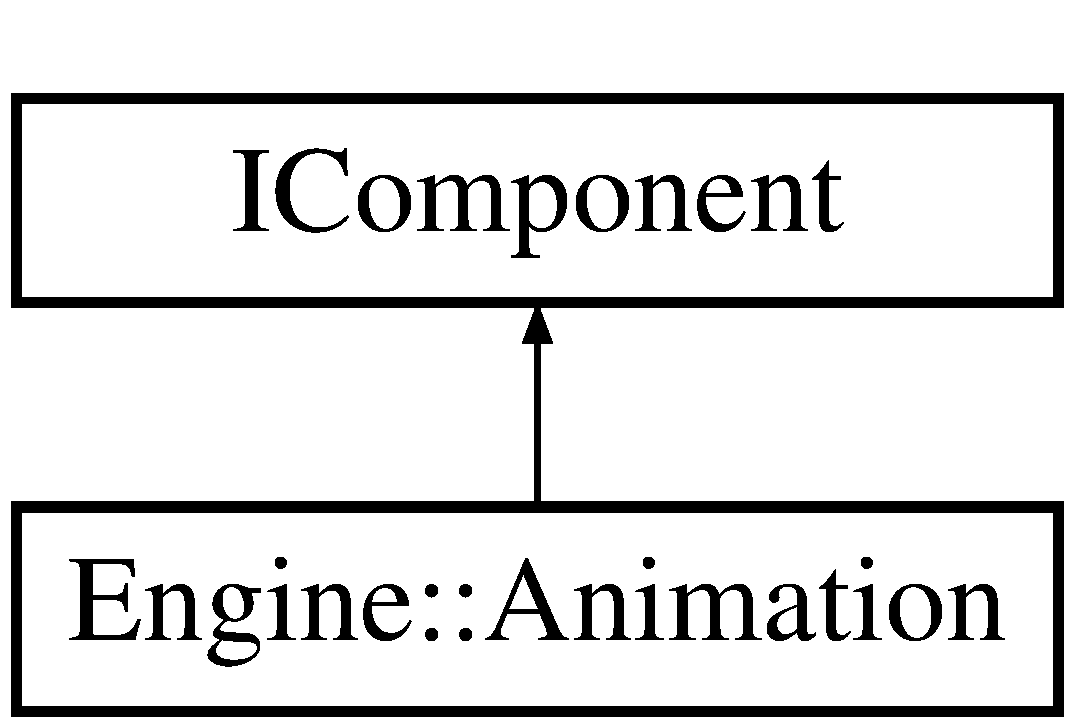
\includegraphics[height=2.000000cm]{classEngine_1_1Animation}
\end{center}
\end{figure}
\subsection*{Public Member Functions}
\begin{DoxyCompactItemize}
\item 
\hyperlink{classEngine_1_1Animation_a83f0a16cef7117f187ad596de38dd9d6}{Animation} ()
\begin{DoxyCompactList}\small\item\em \hyperlink{classEngine_1_1Animation}{Animation}. \end{DoxyCompactList}\item 
\hyperlink{classEngine_1_1Animation_a9c3ef01682e55cb773bedbad9020a759}{Animation} (const std\+::string \&animation\+\_\+name)
\begin{DoxyCompactList}\small\item\em \hyperlink{classEngine_1_1Animation}{Animation}. \end{DoxyCompactList}\item 
\hyperlink{classEngine_1_1Animation_a6462a15fd5a0d0c63ec829727d7c5c40}{$\sim$\+Animation} ()
\item 
void \hyperlink{classEngine_1_1Animation_a243fa7f2a9368bb2cdd22bbeff644ae5}{set\+Frames} (int frame\+\_\+amount)
\begin{DoxyCompactList}\small\item\em set\+Frames \end{DoxyCompactList}\item 
void \hyperlink{classEngine_1_1Animation_aa18bb6bbd6c91370795c45fb63c2a00d}{set\+Frame} (uint frame)
\begin{DoxyCompactList}\small\item\em set\+Frame \end{DoxyCompactList}\item 
void \hyperlink{classEngine_1_1Animation_a572210cbdff12025c70cd928a4aee407}{set\+Bones} (Bones bones)
\begin{DoxyCompactList}\small\item\em set\+Bones \end{DoxyCompactList}\item 
\hypertarget{classEngine_1_1Animation_ab291416fd8a47edcb2e6e34521b2a939}{}void {\bfseries set\+Data} (float $\ast$data, int size)\label{classEngine_1_1Animation_ab291416fd8a47edcb2e6e34521b2a939}

\item 
\hypertarget{classEngine_1_1Animation_a54a61c2c566a014acd9604e770bc81df}{}float $\ast$ {\bfseries get\+Data} (void)\label{classEngine_1_1Animation_a54a61c2c566a014acd9604e770bc81df}

\item 
\hypertarget{classEngine_1_1Animation_a2d915137bb1f8632baa2397b17f517b1}{}void {\bfseries create\+Data} (int size)\label{classEngine_1_1Animation_a2d915137bb1f8632baa2397b17f517b1}

\item 
void \hyperlink{classEngine_1_1Animation_a2678bd4ba646733c450eddea86580b2a}{add\+Bone} (\hyperlink{classEngine_1_1Bone}{Bone} $\ast$bone)
\begin{DoxyCompactList}\small\item\em add\+Bone \end{DoxyCompactList}\item 
int \hyperlink{classEngine_1_1Animation_ac07bf343bc9d9d4affaf521c7a45412e}{get\+Frames} (void)
\begin{DoxyCompactList}\small\item\em get\+Frames \end{DoxyCompactList}\item 
int \hyperlink{classEngine_1_1Animation_abc9b8ad81c5a08dd3248ad9e1126e51a}{get\+Frame} (void)
\begin{DoxyCompactList}\small\item\em get\+Frame \end{DoxyCompactList}\item 
\hyperlink{classEngine_1_1Bone}{Bone} $\ast$ \hyperlink{classEngine_1_1Animation_a733bedc14108ae1ba9b8334459e7e116}{get\+Bone} (const std\+::string \&bone\+\_\+name)
\begin{DoxyCompactList}\small\item\em get\+Bone \end{DoxyCompactList}\item 
Bones \hyperlink{classEngine_1_1Animation_a9976158328cae7a6b48cccee07dece5c}{get\+Bones} (void)
\begin{DoxyCompactList}\small\item\em get\+Bones \end{DoxyCompactList}\item 
int \hyperlink{classEngine_1_1Animation_aefee6093f48f082d0ab7a318a4ebb48f}{get\+Bone\+Index\+By\+Name} (const std\+::string \&bone\+\_\+name)
\begin{DoxyCompactList}\small\item\em get\+Bone\+Index\+By\+Name \end{DoxyCompactList}\item 
void \hyperlink{classEngine_1_1Animation_aecf4dcf209d4b66e9f53585c920b19cb}{Loop} (void)
\begin{DoxyCompactList}\small\item\em Loop. \end{DoxyCompactList}\item 
D\+E\+P\+R\+E\+C\+A\+T\+E\+D void \hyperlink{classEngine_1_1Animation_ab83074cf68569086283113b7b9f7e14b}{Bind\+Matricen} (\hyperlink{classEngine_1_1IShader}{I\+Shader} $\ast$shader)
\begin{DoxyCompactList}\small\item\em send\+Matricen \end{DoxyCompactList}\item 
void \hyperlink{classEngine_1_1Animation_a3a62559d6095b1526b1a8ba0880ef480}{set\+Transforms} (Transform\+Map map)
\begin{DoxyCompactList}\small\item\em set\+Transforms \end{DoxyCompactList}\item 
\hypertarget{classEngine_1_1Animation_a1085ad0d555b1a2b50142e74eeef1807}{}Transform\+Map {\bfseries get\+Transforms} (void)\label{classEngine_1_1Animation_a1085ad0d555b1a2b50142e74eeef1807}

\item 
\hypertarget{classEngine_1_1Animation_a436db3490f71fbb50244ab149b2b861e}{}void {\bfseries set\+Animation\+Name} (const std\+::string \&animation\+\_\+name)\label{classEngine_1_1Animation_a436db3490f71fbb50244ab149b2b861e}

\end{DoxyCompactItemize}


\subsection{Detailed Description}
The \hyperlink{classEngine_1_1Animation}{Animation} class. 

Save \hyperlink{classEngine_1_1Animation}{Animation} Data 

\subsection{Constructor \& Destructor Documentation}
\hypertarget{classEngine_1_1Animation_a83f0a16cef7117f187ad596de38dd9d6}{}\index{Engine\+::\+Animation@{Engine\+::\+Animation}!Animation@{Animation}}
\index{Animation@{Animation}!Engine\+::\+Animation@{Engine\+::\+Animation}}
\subsubsection[{Animation()}]{\setlength{\rightskip}{0pt plus 5cm}Animation\+::\+Animation (
\begin{DoxyParamCaption}
{}
\end{DoxyParamCaption}
)}\label{classEngine_1_1Animation_a83f0a16cef7117f187ad596de38dd9d6}


\hyperlink{classEngine_1_1Animation}{Animation}. 

Default \hyperlink{classEngine_1_1Animation}{Animation} Constructor \hypertarget{classEngine_1_1Animation_a9c3ef01682e55cb773bedbad9020a759}{}\index{Engine\+::\+Animation@{Engine\+::\+Animation}!Animation@{Animation}}
\index{Animation@{Animation}!Engine\+::\+Animation@{Engine\+::\+Animation}}
\subsubsection[{Animation(const std\+::string \&animation\+\_\+name)}]{\setlength{\rightskip}{0pt plus 5cm}Engine\+::\+Animation\+::\+Animation (
\begin{DoxyParamCaption}
\item[{const std\+::string \&}]{animation\+\_\+name}
\end{DoxyParamCaption}
)}\label{classEngine_1_1Animation_a9c3ef01682e55cb773bedbad9020a759}


\hyperlink{classEngine_1_1Animation}{Animation}. 

\hyperlink{classEngine_1_1Animation}{Animation} Constructor with \hyperlink{classEngine_1_1Animation}{Animation} name 
\begin{DoxyParams}{Parameters}
{\em animation\+\_\+name} & \\
\hline
\end{DoxyParams}
\hypertarget{classEngine_1_1Animation_a6462a15fd5a0d0c63ec829727d7c5c40}{}\index{Engine\+::\+Animation@{Engine\+::\+Animation}!````~Animation@{$\sim$\+Animation}}
\index{````~Animation@{$\sim$\+Animation}!Engine\+::\+Animation@{Engine\+::\+Animation}}
\subsubsection[{$\sim$\+Animation()}]{\setlength{\rightskip}{0pt plus 5cm}Engine\+::\+Animation\+::$\sim$\+Animation (
\begin{DoxyParamCaption}
{}
\end{DoxyParamCaption}
)\hspace{0.3cm}{\ttfamily [inline]}}\label{classEngine_1_1Animation_a6462a15fd5a0d0c63ec829727d7c5c40}
Default \hyperlink{classEngine_1_1Animation}{Animation} Destructor 

\subsection{Member Function Documentation}
\hypertarget{classEngine_1_1Animation_a2678bd4ba646733c450eddea86580b2a}{}\index{Engine\+::\+Animation@{Engine\+::\+Animation}!add\+Bone@{add\+Bone}}
\index{add\+Bone@{add\+Bone}!Engine\+::\+Animation@{Engine\+::\+Animation}}
\subsubsection[{add\+Bone(\+Bone $\ast$bone)}]{\setlength{\rightskip}{0pt plus 5cm}void Animation\+::add\+Bone (
\begin{DoxyParamCaption}
\item[{{\bf Bone} $\ast$}]{bone}
\end{DoxyParamCaption}
)}\label{classEngine_1_1Animation_a2678bd4ba646733c450eddea86580b2a}


add\+Bone 

Add a \hyperlink{classEngine_1_1Bone}{Bone} 
\begin{DoxyParams}{Parameters}
{\em bone} & \\
\hline
\end{DoxyParams}
\hypertarget{classEngine_1_1Animation_ab83074cf68569086283113b7b9f7e14b}{}\index{Engine\+::\+Animation@{Engine\+::\+Animation}!Bind\+Matricen@{Bind\+Matricen}}
\index{Bind\+Matricen@{Bind\+Matricen}!Engine\+::\+Animation@{Engine\+::\+Animation}}
\subsubsection[{Bind\+Matricen(\+I\+Shader $\ast$shader)}]{\setlength{\rightskip}{0pt plus 5cm}void Animation\+::\+Bind\+Matricen (
\begin{DoxyParamCaption}
\item[{{\bf I\+Shader} $\ast$}]{shader}
\end{DoxyParamCaption}
)}\label{classEngine_1_1Animation_ab83074cf68569086283113b7b9f7e14b}


send\+Matricen 

Bind \hyperlink{classEngine_1_1Animation}{Animation} Matricen to \hyperlink{classEngine_1_1Shader}{Shader} 
\begin{DoxyParams}{Parameters}
{\em shader} & \\
\hline
\end{DoxyParams}
\hypertarget{classEngine_1_1Animation_a733bedc14108ae1ba9b8334459e7e116}{}\index{Engine\+::\+Animation@{Engine\+::\+Animation}!get\+Bone@{get\+Bone}}
\index{get\+Bone@{get\+Bone}!Engine\+::\+Animation@{Engine\+::\+Animation}}
\subsubsection[{get\+Bone(const std\+::string \&bone\+\_\+name)}]{\setlength{\rightskip}{0pt plus 5cm}{\bf Bone} $\ast$ Animation\+::get\+Bone (
\begin{DoxyParamCaption}
\item[{const std\+::string \&}]{bone\+\_\+name}
\end{DoxyParamCaption}
)}\label{classEngine_1_1Animation_a733bedc14108ae1ba9b8334459e7e116}


get\+Bone 

Return a Single \hyperlink{classEngine_1_1Bone}{Bone} 
\begin{DoxyParams}{Parameters}
{\em bone\+\_\+name} & \\
\hline
\end{DoxyParams}
\begin{DoxyReturn}{Returns}

\end{DoxyReturn}
\hypertarget{classEngine_1_1Animation_aefee6093f48f082d0ab7a318a4ebb48f}{}\index{Engine\+::\+Animation@{Engine\+::\+Animation}!get\+Bone\+Index\+By\+Name@{get\+Bone\+Index\+By\+Name}}
\index{get\+Bone\+Index\+By\+Name@{get\+Bone\+Index\+By\+Name}!Engine\+::\+Animation@{Engine\+::\+Animation}}
\subsubsection[{get\+Bone\+Index\+By\+Name(const std\+::string \&bone\+\_\+name)}]{\setlength{\rightskip}{0pt plus 5cm}int Animation\+::get\+Bone\+Index\+By\+Name (
\begin{DoxyParamCaption}
\item[{const std\+::string \&}]{bone\+\_\+name}
\end{DoxyParamCaption}
)}\label{classEngine_1_1Animation_aefee6093f48f082d0ab7a318a4ebb48f}


get\+Bone\+Index\+By\+Name 

Return \hyperlink{classEngine_1_1Bone}{Bone} Index Number by Name 
\begin{DoxyParams}{Parameters}
{\em bone\+\_\+name} & \\
\hline
\end{DoxyParams}
\begin{DoxyReturn}{Returns}

\end{DoxyReturn}
\hypertarget{classEngine_1_1Animation_a9976158328cae7a6b48cccee07dece5c}{}\index{Engine\+::\+Animation@{Engine\+::\+Animation}!get\+Bones@{get\+Bones}}
\index{get\+Bones@{get\+Bones}!Engine\+::\+Animation@{Engine\+::\+Animation}}
\subsubsection[{get\+Bones(void)}]{\setlength{\rightskip}{0pt plus 5cm}Bones Animation\+::get\+Bones (
\begin{DoxyParamCaption}
\item[{void}]{}
\end{DoxyParamCaption}
)}\label{classEngine_1_1Animation_a9976158328cae7a6b48cccee07dece5c}


get\+Bones 

Return all Bones \begin{DoxyReturn}{Returns}

\end{DoxyReturn}
\hypertarget{classEngine_1_1Animation_abc9b8ad81c5a08dd3248ad9e1126e51a}{}\index{Engine\+::\+Animation@{Engine\+::\+Animation}!get\+Frame@{get\+Frame}}
\index{get\+Frame@{get\+Frame}!Engine\+::\+Animation@{Engine\+::\+Animation}}
\subsubsection[{get\+Frame(void)}]{\setlength{\rightskip}{0pt plus 5cm}int Animation\+::get\+Frame (
\begin{DoxyParamCaption}
\item[{void}]{}
\end{DoxyParamCaption}
)}\label{classEngine_1_1Animation_abc9b8ad81c5a08dd3248ad9e1126e51a}


get\+Frame 

Return currently \hyperlink{classEngine_1_1Animation}{Animation} Frame Number \begin{DoxyReturn}{Returns}

\end{DoxyReturn}
\hypertarget{classEngine_1_1Animation_ac07bf343bc9d9d4affaf521c7a45412e}{}\index{Engine\+::\+Animation@{Engine\+::\+Animation}!get\+Frames@{get\+Frames}}
\index{get\+Frames@{get\+Frames}!Engine\+::\+Animation@{Engine\+::\+Animation}}
\subsubsection[{get\+Frames(void)}]{\setlength{\rightskip}{0pt plus 5cm}int Animation\+::get\+Frames (
\begin{DoxyParamCaption}
\item[{void}]{}
\end{DoxyParamCaption}
)}\label{classEngine_1_1Animation_ac07bf343bc9d9d4affaf521c7a45412e}


get\+Frames 

Return max. frames \begin{DoxyReturn}{Returns}

\end{DoxyReturn}
\hypertarget{classEngine_1_1Animation_aecf4dcf209d4b66e9f53585c920b19cb}{}\index{Engine\+::\+Animation@{Engine\+::\+Animation}!Loop@{Loop}}
\index{Loop@{Loop}!Engine\+::\+Animation@{Engine\+::\+Animation}}
\subsubsection[{Loop(void)}]{\setlength{\rightskip}{0pt plus 5cm}void Animation\+::\+Loop (
\begin{DoxyParamCaption}
\item[{void}]{}
\end{DoxyParamCaption}
)}\label{classEngine_1_1Animation_aecf4dcf209d4b66e9f53585c920b19cb}


Loop. 

\hyperlink{classEngine_1_1Animation}{Animation} Loop \hypertarget{classEngine_1_1Animation_a572210cbdff12025c70cd928a4aee407}{}\index{Engine\+::\+Animation@{Engine\+::\+Animation}!set\+Bones@{set\+Bones}}
\index{set\+Bones@{set\+Bones}!Engine\+::\+Animation@{Engine\+::\+Animation}}
\subsubsection[{set\+Bones(\+Bones bones)}]{\setlength{\rightskip}{0pt plus 5cm}void Animation\+::set\+Bones (
\begin{DoxyParamCaption}
\item[{Bones}]{bones}
\end{DoxyParamCaption}
)}\label{classEngine_1_1Animation_a572210cbdff12025c70cd928a4aee407}


set\+Bones 

set Bones 
\begin{DoxyParams}{Parameters}
{\em bones} & \\
\hline
\end{DoxyParams}
\hypertarget{classEngine_1_1Animation_aa18bb6bbd6c91370795c45fb63c2a00d}{}\index{Engine\+::\+Animation@{Engine\+::\+Animation}!set\+Frame@{set\+Frame}}
\index{set\+Frame@{set\+Frame}!Engine\+::\+Animation@{Engine\+::\+Animation}}
\subsubsection[{set\+Frame(uint frame)}]{\setlength{\rightskip}{0pt plus 5cm}void Animation\+::set\+Frame (
\begin{DoxyParamCaption}
\item[{uint}]{frame}
\end{DoxyParamCaption}
)}\label{classEngine_1_1Animation_aa18bb6bbd6c91370795c45fb63c2a00d}


set\+Frame 

Set currently \hyperlink{classEngine_1_1Animation}{Animation} Frame Number 
\begin{DoxyParams}{Parameters}
{\em frame} & \\
\hline
\end{DoxyParams}
\hypertarget{classEngine_1_1Animation_a243fa7f2a9368bb2cdd22bbeff644ae5}{}\index{Engine\+::\+Animation@{Engine\+::\+Animation}!set\+Frames@{set\+Frames}}
\index{set\+Frames@{set\+Frames}!Engine\+::\+Animation@{Engine\+::\+Animation}}
\subsubsection[{set\+Frames(int frame\+\_\+amount)}]{\setlength{\rightskip}{0pt plus 5cm}void Animation\+::set\+Frames (
\begin{DoxyParamCaption}
\item[{int}]{frame\+\_\+amount}
\end{DoxyParamCaption}
)}\label{classEngine_1_1Animation_a243fa7f2a9368bb2cdd22bbeff644ae5}


set\+Frames 

Set max. Frames 
\begin{DoxyParams}{Parameters}
{\em frame\+\_\+amount} & \\
\hline
\end{DoxyParams}
\hypertarget{classEngine_1_1Animation_a3a62559d6095b1526b1a8ba0880ef480}{}\index{Engine\+::\+Animation@{Engine\+::\+Animation}!set\+Transforms@{set\+Transforms}}
\index{set\+Transforms@{set\+Transforms}!Engine\+::\+Animation@{Engine\+::\+Animation}}
\subsubsection[{set\+Transforms(\+Transform\+Map map)}]{\setlength{\rightskip}{0pt plus 5cm}void Animation\+::set\+Transforms (
\begin{DoxyParamCaption}
\item[{Transform\+Map}]{map}
\end{DoxyParamCaption}
)}\label{classEngine_1_1Animation_a3a62559d6095b1526b1a8ba0880ef480}


set\+Transforms 

Add Transformations 
\begin{DoxyParams}{Parameters}
{\em map} & \\
\hline
\end{DoxyParams}


The documentation for this class was generated from the following files\+:\begin{DoxyCompactItemize}
\item 
include/\+Container/animation.\+h\item 
Container/Animation.\+cpp\end{DoxyCompactItemize}

\hypertarget{classEngine_1_1AnimationLoader}{}\section{Engine\+:\+:Animation\+Loader Class Reference}
\label{classEngine_1_1AnimationLoader}\index{Engine\+::\+Animation\+Loader@{Engine\+::\+Animation\+Loader}}


The \hyperlink{classEngine_1_1AnimationLoader}{Animation\+Loader} is a interface class for custom Loader specifically for Animations.  




{\ttfamily \#include $<$animationmanager.\+h$>$}

Inheritance diagram for Engine\+:\+:Animation\+Loader\+:\begin{figure}[H]
\begin{center}
\leavevmode
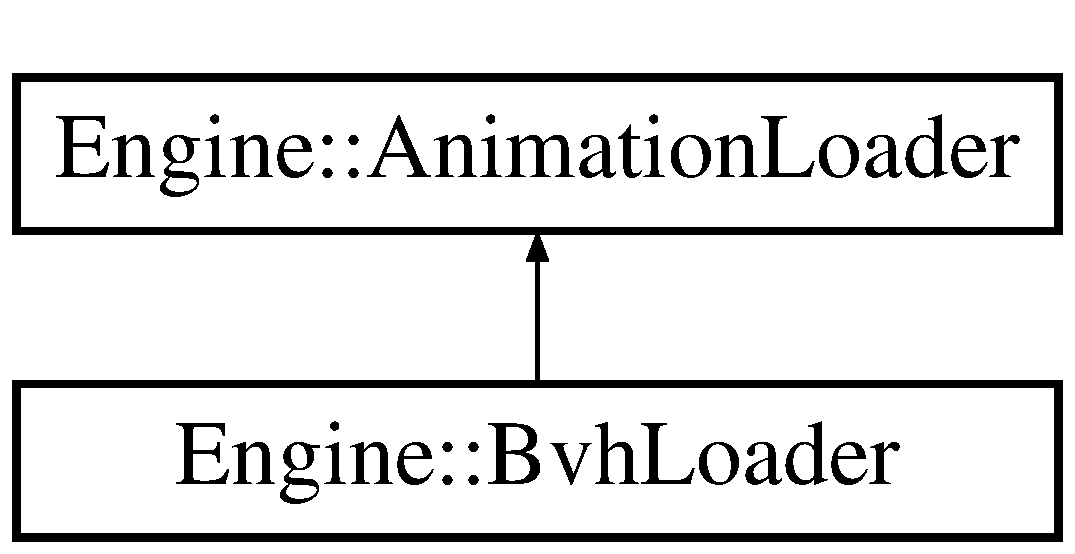
\includegraphics[height=2.000000cm]{classEngine_1_1AnimationLoader}
\end{center}
\end{figure}
\subsection*{Public Member Functions}
\begin{DoxyCompactItemize}
\item 
\hypertarget{classEngine_1_1AnimationLoader_a063c535a3cecc06caaae1833325bde07}{}{\bfseries Animation\+Loader} (const std\+::string \&extension)\label{classEngine_1_1AnimationLoader_a063c535a3cecc06caaae1833325bde07}

\item 
virtual void \hyperlink{classEngine_1_1AnimationLoader_ac077ab98aa64ab4eae5e7ca47d7d48f1}{Read\+File} (const std\+::string \&motion\+\_\+file, \hyperlink{classEngine_1_1NodeAnimScene}{Node\+Anim\+Scene} $\ast$node\+\_\+anim\+\_\+scene)=0
\begin{DoxyCompactList}\small\item\em Read\+File. \end{DoxyCompactList}\end{DoxyCompactItemize}
\subsection*{Protected Attributes}
\begin{DoxyCompactItemize}
\item 
unsigned int \hyperlink{classEngine_1_1AnimationLoader_ae6851f3980f517aa5eb62b9bb9f16ed0}{m\+Flags}
\item 
std\+::string \hyperlink{classEngine_1_1AnimationLoader_a0507d3a76b6f33f05be9fc789138c508}{m\+Extension}
\end{DoxyCompactItemize}
\subsection*{Friends}
\begin{DoxyCompactItemize}
\item 
\hypertarget{classEngine_1_1AnimationLoader_a00b7f00c1e25e81e518e5faa334dbe66}{}class {\bfseries Animation\+Manager}\label{classEngine_1_1AnimationLoader_a00b7f00c1e25e81e518e5faa334dbe66}

\end{DoxyCompactItemize}


\subsection{Detailed Description}
The \hyperlink{classEngine_1_1AnimationLoader}{Animation\+Loader} is a interface class for custom Loader specifically for Animations. 

\subsection{Member Function Documentation}
\hypertarget{classEngine_1_1AnimationLoader_ac077ab98aa64ab4eae5e7ca47d7d48f1}{}\index{Engine\+::\+Animation\+Loader@{Engine\+::\+Animation\+Loader}!Read\+File@{Read\+File}}
\index{Read\+File@{Read\+File}!Engine\+::\+Animation\+Loader@{Engine\+::\+Animation\+Loader}}
\subsubsection[{Read\+File(const std\+::string \&motion\+\_\+file, Node\+Anim\+Scene $\ast$node\+\_\+anim\+\_\+scene)=0}]{\setlength{\rightskip}{0pt plus 5cm}virtual void Engine\+::\+Animation\+Loader\+::\+Read\+File (
\begin{DoxyParamCaption}
\item[{const std\+::string \&}]{motion\+\_\+file, }
\item[{{\bf Node\+Anim\+Scene} $\ast$}]{node\+\_\+anim\+\_\+scene}
\end{DoxyParamCaption}
)\hspace{0.3cm}{\ttfamily [pure virtual]}}\label{classEngine_1_1AnimationLoader_ac077ab98aa64ab4eae5e7ca47d7d48f1}


Read\+File. 

Read Motion\+File and Save data into anim\+\_\+scene 
\begin{DoxyParams}{Parameters}
{\em motion\+\_\+file} & \\
\hline
{\em node\+\_\+anim\+\_\+scene} & \\
\hline
\end{DoxyParams}


\subsection{Member Data Documentation}
\hypertarget{classEngine_1_1AnimationLoader_a0507d3a76b6f33f05be9fc789138c508}{}\index{Engine\+::\+Animation\+Loader@{Engine\+::\+Animation\+Loader}!m\+Extension@{m\+Extension}}
\index{m\+Extension@{m\+Extension}!Engine\+::\+Animation\+Loader@{Engine\+::\+Animation\+Loader}}
\subsubsection[{m\+Extension}]{\setlength{\rightskip}{0pt plus 5cm}std\+::string Engine\+::\+Animation\+Loader\+::m\+Extension\hspace{0.3cm}{\ttfamily [protected]}}\label{classEngine_1_1AnimationLoader_a0507d3a76b6f33f05be9fc789138c508}
actually Loader extension \hypertarget{classEngine_1_1AnimationLoader_ae6851f3980f517aa5eb62b9bb9f16ed0}{}\index{Engine\+::\+Animation\+Loader@{Engine\+::\+Animation\+Loader}!m\+Flags@{m\+Flags}}
\index{m\+Flags@{m\+Flags}!Engine\+::\+Animation\+Loader@{Engine\+::\+Animation\+Loader}}
\subsubsection[{m\+Flags}]{\setlength{\rightskip}{0pt plus 5cm}unsigned int Engine\+::\+Animation\+Loader\+::m\+Flags\hspace{0.3cm}{\ttfamily [protected]}}\label{classEngine_1_1AnimationLoader_ae6851f3980f517aa5eb62b9bb9f16ed0}
actually Loader flags 

The documentation for this class was generated from the following files\+:\begin{DoxyCompactItemize}
\item 
include/\+Manager/animationmanager.\+h\item 
Engine/\+Manager/Animation\+Manager.\+cpp\end{DoxyCompactItemize}

\hypertarget{classEngine_1_1AnimationManager}{}\section{Engine\+:\+:Animation\+Manager Class Reference}
\label{classEngine_1_1AnimationManager}\index{Engine\+::\+Animation\+Manager@{Engine\+::\+Animation\+Manager}}


The \hyperlink{classEngine_1_1AnimationManager}{Animation\+Manager} controlled Animations.  




{\ttfamily \#include $<$animationmanager.\+h$>$}

Inheritance diagram for Engine\+:\+:Animation\+Manager\+:\begin{figure}[H]
\begin{center}
\leavevmode
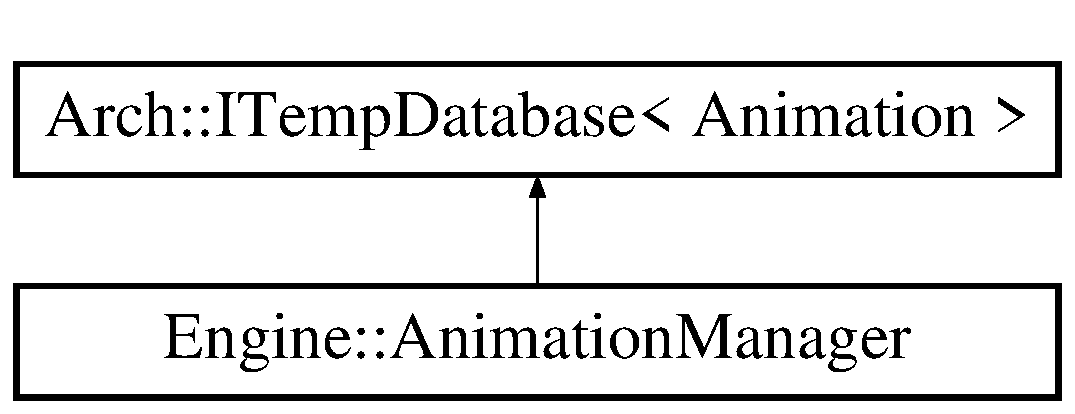
\includegraphics[height=2.000000cm]{classEngine_1_1AnimationManager}
\end{center}
\end{figure}
\subsection*{Public Types}
\begin{DoxyCompactItemize}
\item 
\hypertarget{classEngine_1_1AnimationManager_a3625098c28199094ef82056c22414205}{}using {\bfseries Animation\+Map} = std\+::map$<$ uint, \hyperlink{classEngine_1_1Animation}{Animation} $\ast$ $>$\label{classEngine_1_1AnimationManager_a3625098c28199094ef82056c22414205}

\item 
\hypertarget{classEngine_1_1AnimationManager_a97a8ac1d418ab00715d47d2278e608ab}{}using {\bfseries Anim\+Loader\+List} = std\+::list$<$ \hyperlink{classEngine_1_1AnimationLoader}{Animation\+Loader} $\ast$ $>$\label{classEngine_1_1AnimationManager_a97a8ac1d418ab00715d47d2278e608ab}

\end{DoxyCompactItemize}
\subsection*{Public Member Functions}
\begin{DoxyCompactItemize}
\item 
void \hyperlink{classEngine_1_1AnimationManager_a4d2622e81e065e7d55fe0c127b26ad33}{prepare\+V\+B\+O} (\hyperlink{classEngine_1_1Animation}{Animation} $\ast$anim, \hyperlink{classEngine_1_1Mesh}{Mesh} $\ast$mesh)
\begin{DoxyCompactList}\small\item\em \hyperlink{classEngine_1_1AnimationManager_a4d2622e81e065e7d55fe0c127b26ad33}{Animation\+Manager\+::prepare\+V\+B\+O}. \end{DoxyCompactList}\item 
\hypertarget{classEngine_1_1AnimationManager_a62d0a57ab543057eaf245d37b486a752}{}void {\bfseries Add\+Transformations} (\hyperlink{classEngine_1_1Animation}{Animation} $\ast$anim, \hyperlink{classEngine_1_1Mesh}{Mesh} $\ast$mesh)\label{classEngine_1_1AnimationManager_a62d0a57ab543057eaf245d37b486a752}

\item 
\hyperlink{classEngine_1_1Animation}{Animation} $\ast$ \hyperlink{classEngine_1_1AnimationManager_a9bfe9218d60ae4d9ea5c0911813f7f8d}{create\+Animation} (const std\+::string \&animation\+\_\+name, const std\+::string \&motion\+\_\+file, \hyperlink{classEngine_1_1Mesh}{Mesh} $\ast$mesh)  throw ( std\+::runtime\+\_\+error )
\begin{DoxyCompactList}\small\item\em create\+Animation \end{DoxyCompactList}\item 
\hypertarget{classEngine_1_1AnimationManager_acb671d94e2ddf41b9e0e2e0ee07d51f2}{}void {\bfseries Create\+Bones} (\hyperlink{classEngine_1_1Animation}{Animation} $\ast$animation, const std\+::string \&motion\+\_\+file)\label{classEngine_1_1AnimationManager_acb671d94e2ddf41b9e0e2e0ee07d51f2}

\item 
\hyperlink{classEngine_1_1Animation}{Animation} $\ast$ \hyperlink{classEngine_1_1AnimationManager_aa22f9a6d3b41f702da6c6c2ec5414acc}{get\+Animation} (uint component\+\_\+id)
\begin{DoxyCompactList}\small\item\em get\+Animation \end{DoxyCompactList}\item 
void \hyperlink{classEngine_1_1AnimationManager_ac5aa9b68314681e6b1cc449d259ee277}{destroy} (uint component\+\_\+id)
\begin{DoxyCompactList}\small\item\em remove \end{DoxyCompactList}\item 
const \hyperlink{classEngine_1_1NodeAnimScene}{Node\+Anim\+Scene} $\ast$ \hyperlink{classEngine_1_1AnimationManager_a0314d0b13a86da7ea893333dbb69d833}{Read\+File} (const std\+::string \&motion\+\_\+file, unsigned int flags)
\begin{DoxyCompactList}\small\item\em Read\+File. \end{DoxyCompactList}\item 
bool \hyperlink{classEngine_1_1AnimationManager_a3248d132cea1fdf69d96c2c7d1ffda08}{Is\+Extension\+Supported} (const std\+::string \&extension)
\begin{DoxyCompactList}\small\item\em Is\+Extension\+Supported. \end{DoxyCompactList}\item 
void \hyperlink{classEngine_1_1AnimationManager_a5d5c62435011bb70e8b344700e1a6829}{register\+Loader} (\hyperlink{classEngine_1_1AnimationLoader}{Animation\+Loader} $\ast$loader)
\begin{DoxyCompactList}\small\item\em register\+Loader \end{DoxyCompactList}\end{DoxyCompactItemize}
\subsection*{Protected Member Functions}
\begin{DoxyCompactItemize}
\item 
void \hyperlink{classEngine_1_1AnimationManager_a697b862a65f681654d92b5ea529fd9f4}{add\+Extension\+Support} (const std\+::string \&extension)
\begin{DoxyCompactList}\small\item\em add\+Extension\+Support \end{DoxyCompactList}\item 
void \hyperlink{classEngine_1_1AnimationManager_a5b150fa34470c4221baea6fc94ef2007}{prepare\+Animation} (\hyperlink{classEngine_1_1Animation}{Animation} $\ast$anim, \hyperlink{classEngine_1_1Mesh}{Mesh} $\ast$mesh)
\begin{DoxyCompactList}\small\item\em create\+Bone\+Index \end{DoxyCompactList}\end{DoxyCompactItemize}


\subsection{Detailed Description}
The \hyperlink{classEngine_1_1AnimationManager}{Animation\+Manager} controlled Animations. 

\subsection{Member Function Documentation}
\hypertarget{classEngine_1_1AnimationManager_a697b862a65f681654d92b5ea529fd9f4}{}\index{Engine\+::\+Animation\+Manager@{Engine\+::\+Animation\+Manager}!add\+Extension\+Support@{add\+Extension\+Support}}
\index{add\+Extension\+Support@{add\+Extension\+Support}!Engine\+::\+Animation\+Manager@{Engine\+::\+Animation\+Manager}}
\subsubsection[{add\+Extension\+Support(const std\+::string \&extension)}]{\setlength{\rightskip}{0pt plus 5cm}void Animation\+Manager\+::add\+Extension\+Support (
\begin{DoxyParamCaption}
\item[{const std\+::string \&}]{extension}
\end{DoxyParamCaption}
)\hspace{0.3cm}{\ttfamily [protected]}}\label{classEngine_1_1AnimationManager_a697b862a65f681654d92b5ea529fd9f4}


add\+Extension\+Support 

Add new Extension 
\begin{DoxyParams}{Parameters}
{\em extension} & \\
\hline
\end{DoxyParams}
\hypertarget{classEngine_1_1AnimationManager_a9bfe9218d60ae4d9ea5c0911813f7f8d}{}\index{Engine\+::\+Animation\+Manager@{Engine\+::\+Animation\+Manager}!create\+Animation@{create\+Animation}}
\index{create\+Animation@{create\+Animation}!Engine\+::\+Animation\+Manager@{Engine\+::\+Animation\+Manager}}
\subsubsection[{create\+Animation(const std\+::string \&animation\+\_\+name, const std\+::string \&motion\+\_\+file, Mesh $\ast$mesh)}]{\setlength{\rightskip}{0pt plus 5cm}{\bf Animation} $\ast$ Animation\+Manager\+::create\+Animation (
\begin{DoxyParamCaption}
\item[{const std\+::string \&}]{animation\+\_\+name, }
\item[{const std\+::string \&}]{motion\+\_\+file, }
\item[{{\bf Mesh} $\ast$}]{mesh}
\end{DoxyParamCaption}
) throw  std\+::runtime\+\_\+error) }\label{classEngine_1_1AnimationManager_a9bfe9218d60ae4d9ea5c0911813f7f8d}


create\+Animation 

Create a New \hyperlink{classEngine_1_1Animation}{Animation} with \hyperlink{classEngine_1_1Animation}{Animation} Name \& \hyperlink{classEngine_1_1Animation}{Animation} Motion file


\begin{DoxyParams}{Parameters}
{\em animation\+\_\+name} & \\
\hline
{\em motion\+\_\+file} & \+: (./resource/animation.bvh) \\
\hline
\end{DoxyParams}
\begin{DoxyReturn}{Returns}

\end{DoxyReturn}
\hypertarget{classEngine_1_1AnimationManager_ac5aa9b68314681e6b1cc449d259ee277}{}\index{Engine\+::\+Animation\+Manager@{Engine\+::\+Animation\+Manager}!destroy@{destroy}}
\index{destroy@{destroy}!Engine\+::\+Animation\+Manager@{Engine\+::\+Animation\+Manager}}
\subsubsection[{destroy(uint component\+\_\+id)}]{\setlength{\rightskip}{0pt plus 5cm}void Animation\+Manager\+::destroy (
\begin{DoxyParamCaption}
\item[{uint}]{component\+\_\+id}
\end{DoxyParamCaption}
)}\label{classEngine_1_1AnimationManager_ac5aa9b68314681e6b1cc449d259ee277}


remove 

Destroy \hyperlink{classEngine_1_1Animation}{Animation} 
\begin{DoxyParams}{Parameters}
{\em component\+\_\+id} & \\
\hline
\end{DoxyParams}
\hypertarget{classEngine_1_1AnimationManager_aa22f9a6d3b41f702da6c6c2ec5414acc}{}\index{Engine\+::\+Animation\+Manager@{Engine\+::\+Animation\+Manager}!get\+Animation@{get\+Animation}}
\index{get\+Animation@{get\+Animation}!Engine\+::\+Animation\+Manager@{Engine\+::\+Animation\+Manager}}
\subsubsection[{get\+Animation(uint component\+\_\+id)}]{\setlength{\rightskip}{0pt plus 5cm}{\bf Animation} $\ast$ Animation\+Manager\+::get\+Animation (
\begin{DoxyParamCaption}
\item[{uint}]{component\+\_\+id}
\end{DoxyParamCaption}
)}\label{classEngine_1_1AnimationManager_aa22f9a6d3b41f702da6c6c2ec5414acc}


get\+Animation 

Return \hyperlink{classEngine_1_1Animation}{Animation} by Component I\+D 
\begin{DoxyParams}{Parameters}
{\em component\+\_\+id} & \\
\hline
\end{DoxyParams}
\begin{DoxyReturn}{Returns}

\end{DoxyReturn}
\hypertarget{classEngine_1_1AnimationManager_a3248d132cea1fdf69d96c2c7d1ffda08}{}\index{Engine\+::\+Animation\+Manager@{Engine\+::\+Animation\+Manager}!Is\+Extension\+Supported@{Is\+Extension\+Supported}}
\index{Is\+Extension\+Supported@{Is\+Extension\+Supported}!Engine\+::\+Animation\+Manager@{Engine\+::\+Animation\+Manager}}
\subsubsection[{Is\+Extension\+Supported(const std\+::string \&extension)}]{\setlength{\rightskip}{0pt plus 5cm}bool Animation\+Manager\+::\+Is\+Extension\+Supported (
\begin{DoxyParamCaption}
\item[{const std\+::string \&}]{extension}
\end{DoxyParamCaption}
)}\label{classEngine_1_1AnimationManager_a3248d132cea1fdf69d96c2c7d1ffda08}


Is\+Extension\+Supported. 

Is Extension Supported then return true otherwise is false 
\begin{DoxyParams}{Parameters}
{\em extension} & \+: \char`\"{}.\+bvh\char`\"{} \\
\hline
\end{DoxyParams}
\begin{DoxyReturn}{Returns}

\end{DoxyReturn}
\hypertarget{classEngine_1_1AnimationManager_a5b150fa34470c4221baea6fc94ef2007}{}\index{Engine\+::\+Animation\+Manager@{Engine\+::\+Animation\+Manager}!prepare\+Animation@{prepare\+Animation}}
\index{prepare\+Animation@{prepare\+Animation}!Engine\+::\+Animation\+Manager@{Engine\+::\+Animation\+Manager}}
\subsubsection[{prepare\+Animation(\+Animation $\ast$anim, Mesh $\ast$mesh)}]{\setlength{\rightskip}{0pt plus 5cm}void Animation\+Manager\+::prepare\+Animation (
\begin{DoxyParamCaption}
\item[{{\bf Animation} $\ast$}]{anim, }
\item[{{\bf Mesh} $\ast$}]{mesh}
\end{DoxyParamCaption}
)\hspace{0.3cm}{\ttfamily [protected]}}\label{classEngine_1_1AnimationManager_a5b150fa34470c4221baea6fc94ef2007}


create\+Bone\+Index 

Create a \hyperlink{classEngine_1_1Bone}{Bone} Index for the \hyperlink{classEngine_1_1Animation}{Animation} \hyperlink{classEngine_1_1Shader}{Shader} 
\begin{DoxyParams}{Parameters}
{\em anim} & \\
\hline
{\em mesh} & \\
\hline
\end{DoxyParams}
\hypertarget{classEngine_1_1AnimationManager_a4d2622e81e065e7d55fe0c127b26ad33}{}\index{Engine\+::\+Animation\+Manager@{Engine\+::\+Animation\+Manager}!prepare\+V\+B\+O@{prepare\+V\+B\+O}}
\index{prepare\+V\+B\+O@{prepare\+V\+B\+O}!Engine\+::\+Animation\+Manager@{Engine\+::\+Animation\+Manager}}
\subsubsection[{prepare\+V\+B\+O(\+Animation $\ast$anim, Mesh $\ast$mesh)}]{\setlength{\rightskip}{0pt plus 5cm}void Animation\+Manager\+::prepare\+V\+B\+O (
\begin{DoxyParamCaption}
\item[{{\bf Animation} $\ast$}]{anim, }
\item[{{\bf Mesh} $\ast$}]{mesh}
\end{DoxyParamCaption}
)}\label{classEngine_1_1AnimationManager_a4d2622e81e065e7d55fe0c127b26ad33}


\hyperlink{classEngine_1_1AnimationManager_a4d2622e81e065e7d55fe0c127b26ad33}{Animation\+Manager\+::prepare\+V\+B\+O}. 

Update Shadow V\+B\+O -\/ C\+P\+U Skinning 
\begin{DoxyParams}{Parameters}
{\em anim} & \\
\hline
{\em mesh} & \\
\hline
\end{DoxyParams}
\hypertarget{classEngine_1_1AnimationManager_a0314d0b13a86da7ea893333dbb69d833}{}\index{Engine\+::\+Animation\+Manager@{Engine\+::\+Animation\+Manager}!Read\+File@{Read\+File}}
\index{Read\+File@{Read\+File}!Engine\+::\+Animation\+Manager@{Engine\+::\+Animation\+Manager}}
\subsubsection[{Read\+File(const std\+::string \&motion\+\_\+file, unsigned int flags)}]{\setlength{\rightskip}{0pt plus 5cm}const {\bf Node\+Anim\+Scene} $\ast$ Animation\+Manager\+::\+Read\+File (
\begin{DoxyParamCaption}
\item[{const std\+::string \&}]{motion\+\_\+file, }
\item[{unsigned int}]{flags}
\end{DoxyParamCaption}
)}\label{classEngine_1_1AnimationManager_a0314d0b13a86da7ea893333dbb69d833}


Read\+File. 

Read \hyperlink{classEngine_1_1Animation}{Animation} File 
\begin{DoxyParams}{Parameters}
{\em motion\+\_\+file} & \\
\hline
{\em flags} & \\
\hline
\end{DoxyParams}
\begin{DoxyReturn}{Returns}
\hyperlink{classEngine_1_1NodeAnimScene}{Node\+Anim\+Scene} 
\end{DoxyReturn}
\hypertarget{classEngine_1_1AnimationManager_a5d5c62435011bb70e8b344700e1a6829}{}\index{Engine\+::\+Animation\+Manager@{Engine\+::\+Animation\+Manager}!register\+Loader@{register\+Loader}}
\index{register\+Loader@{register\+Loader}!Engine\+::\+Animation\+Manager@{Engine\+::\+Animation\+Manager}}
\subsubsection[{register\+Loader(\+Animation\+Loader $\ast$loader)}]{\setlength{\rightskip}{0pt plus 5cm}void Animation\+Manager\+::register\+Loader (
\begin{DoxyParamCaption}
\item[{{\bf Animation\+Loader} $\ast$}]{loader}
\end{DoxyParamCaption}
)}\label{classEngine_1_1AnimationManager_a5d5c62435011bb70e8b344700e1a6829}


register\+Loader 

Register new \hyperlink{classEngine_1_1AnimationLoader}{Animation\+Loader} 
\begin{DoxyParams}{Parameters}
{\em loader} & \\
\hline
\end{DoxyParams}


The documentation for this class was generated from the following files\+:\begin{DoxyCompactItemize}
\item 
include/\+Manager/animationmanager.\+h\item 
Engine/\+Manager/Animation\+Manager.\+cpp\end{DoxyCompactItemize}

\hypertarget{classEngine_1_1Attribute}{}\section{Engine\+:\+:Attribute Class Reference}
\label{classEngine_1_1Attribute}\index{Engine\+::\+Attribute@{Engine\+::\+Attribute}}


The \hyperlink{classEngine_1_1Attribute}{Attribute} class.  




{\ttfamily \#include $<$attribute.\+h$>$}

Inheritance diagram for Engine\+:\+:Attribute\+:\begin{figure}[H]
\begin{center}
\leavevmode
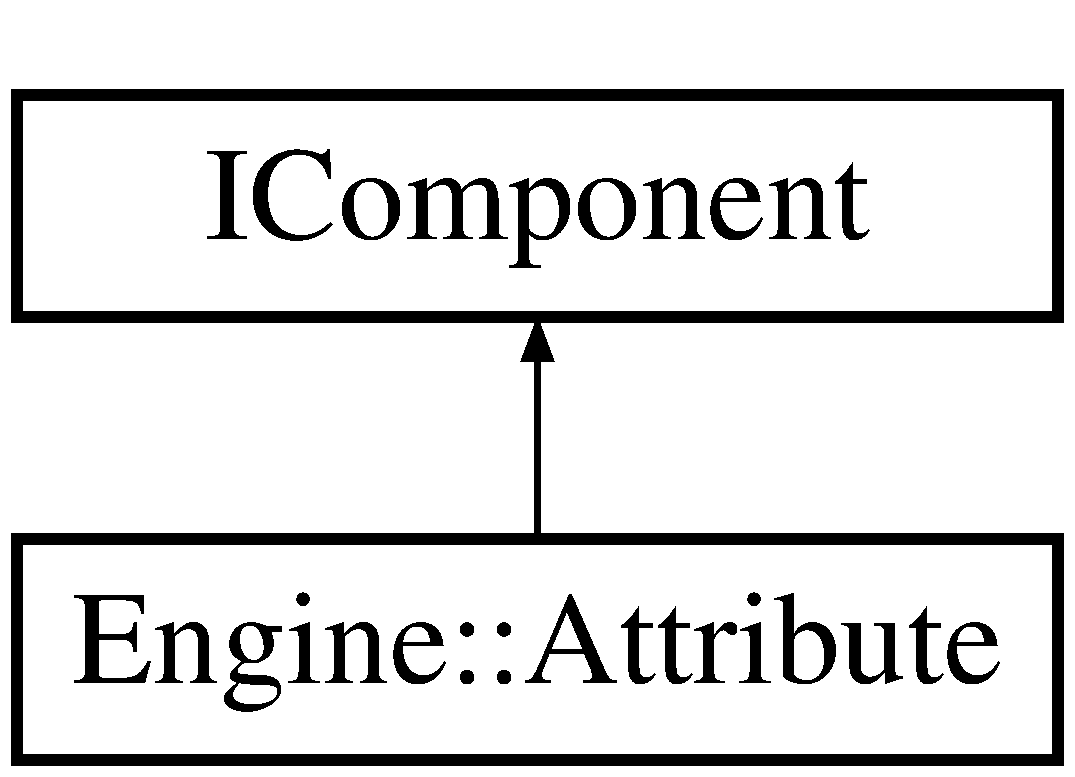
\includegraphics[height=2.000000cm]{classEngine_1_1Attribute}
\end{center}
\end{figure}
\subsection*{Public Member Functions}
\begin{DoxyCompactItemize}
\item 
void \hyperlink{classEngine_1_1Attribute_ac5f7a56bfd8659660a01d57c77b09854}{add\+Attribut} (int attribute\+\_\+id)
\begin{DoxyCompactList}\small\item\em add\+Attribut \end{DoxyCompactList}\item 
bool \hyperlink{classEngine_1_1Attribute_a631efe6abc46594846c900fee4f4a645}{has\+Attribut} (int attribute\+\_\+id)
\begin{DoxyCompactList}\small\item\em has\+Attribut \end{DoxyCompactList}\item 
void \hyperlink{classEngine_1_1Attribute_a412e67db78340d50a1ce0107c36c467c}{remove} (int attribute\+\_\+id)
\begin{DoxyCompactList}\small\item\em remove \end{DoxyCompactList}\item 
Attr\+Index\+List \hyperlink{classEngine_1_1Attribute_a6e884961a7a4798b21dafd6d991b3506}{get\+Attr\+List} (void)
\begin{DoxyCompactList}\small\item\em get\+Attr\+List \end{DoxyCompactList}\end{DoxyCompactItemize}


\subsection{Detailed Description}
The \hyperlink{classEngine_1_1Attribute}{Attribute} class. 

Saved \hyperlink{classEngine_1_1Attribute}{Attribute} values -\/ only Integers 

\subsection{Member Function Documentation}
\hypertarget{classEngine_1_1Attribute_ac5f7a56bfd8659660a01d57c77b09854}{}\index{Engine\+::\+Attribute@{Engine\+::\+Attribute}!add\+Attribut@{add\+Attribut}}
\index{add\+Attribut@{add\+Attribut}!Engine\+::\+Attribute@{Engine\+::\+Attribute}}
\subsubsection[{add\+Attribut(int attribute\+\_\+id)}]{\setlength{\rightskip}{0pt plus 5cm}void Attribute\+::add\+Attribut (
\begin{DoxyParamCaption}
\item[{int}]{attribute\+\_\+id}
\end{DoxyParamCaption}
)}\label{classEngine_1_1Attribute_ac5f7a56bfd8659660a01d57c77b09854}


add\+Attribut 

Set a \hyperlink{classEngine_1_1Attribute}{Attribute} Number 
\begin{DoxyParams}{Parameters}
{\em attribute\+\_\+id} & \\
\hline
\end{DoxyParams}
\hypertarget{classEngine_1_1Attribute_a6e884961a7a4798b21dafd6d991b3506}{}\index{Engine\+::\+Attribute@{Engine\+::\+Attribute}!get\+Attr\+List@{get\+Attr\+List}}
\index{get\+Attr\+List@{get\+Attr\+List}!Engine\+::\+Attribute@{Engine\+::\+Attribute}}
\subsubsection[{get\+Attr\+List(void)}]{\setlength{\rightskip}{0pt plus 5cm}Attr\+Index\+List Attribute\+::get\+Attr\+List (
\begin{DoxyParamCaption}
\item[{void}]{}
\end{DoxyParamCaption}
)}\label{classEngine_1_1Attribute_a6e884961a7a4798b21dafd6d991b3506}


get\+Attr\+List 

Return \hyperlink{classEngine_1_1Attribute}{Attribute} \begin{DoxyReturn}{Returns}

\end{DoxyReturn}
\hypertarget{classEngine_1_1Attribute_a631efe6abc46594846c900fee4f4a645}{}\index{Engine\+::\+Attribute@{Engine\+::\+Attribute}!has\+Attribut@{has\+Attribut}}
\index{has\+Attribut@{has\+Attribut}!Engine\+::\+Attribute@{Engine\+::\+Attribute}}
\subsubsection[{has\+Attribut(int attribute\+\_\+id)}]{\setlength{\rightskip}{0pt plus 5cm}bool Attribute\+::has\+Attribut (
\begin{DoxyParamCaption}
\item[{int}]{attribute\+\_\+id}
\end{DoxyParamCaption}
)}\label{classEngine_1_1Attribute_a631efe6abc46594846c900fee4f4a645}


has\+Attribut 

Return true , if attribute\+\_\+id exists 
\begin{DoxyParams}{Parameters}
{\em attribute\+\_\+id} & \\
\hline
\end{DoxyParams}
\begin{DoxyReturn}{Returns}

\end{DoxyReturn}
\hypertarget{classEngine_1_1Attribute_a412e67db78340d50a1ce0107c36c467c}{}\index{Engine\+::\+Attribute@{Engine\+::\+Attribute}!remove@{remove}}
\index{remove@{remove}!Engine\+::\+Attribute@{Engine\+::\+Attribute}}
\subsubsection[{remove(int attribute\+\_\+id)}]{\setlength{\rightskip}{0pt plus 5cm}void Attribute\+::remove (
\begin{DoxyParamCaption}
\item[{int}]{attribute\+\_\+id}
\end{DoxyParamCaption}
)}\label{classEngine_1_1Attribute_a412e67db78340d50a1ce0107c36c467c}


remove 

Remove attribute\+\_\+id from list 
\begin{DoxyParams}{Parameters}
{\em attribute\+\_\+id} & \\
\hline
\end{DoxyParams}


The documentation for this class was generated from the following files\+:\begin{DoxyCompactItemize}
\item 
include/\+Container/attribute.\+h\item 
Container/Attribute.\+cpp\end{DoxyCompactItemize}

\hypertarget{structEngine_1_1AttributeCmd}{}\section{Engine\+:\+:Attribute\+Cmd Struct Reference}
\label{structEngine_1_1AttributeCmd}\index{Engine\+::\+Attribute\+Cmd@{Engine\+::\+Attribute\+Cmd}}


The \hyperlink{structEngine_1_1AttributeCmd}{Attribute\+Cmd} struct.  




{\ttfamily \#include $<$glvertexarrayobject.\+h$>$}

\subsection*{Public Attributes}
\begin{DoxyCompactItemize}
\item 
\hypertarget{structEngine_1_1AttributeCmd_a1c3a19b8ccb5ea15422ccad7b86020fd}{}uint {\bfseries attribute\+\_\+id}\label{structEngine_1_1AttributeCmd_a1c3a19b8ccb5ea15422ccad7b86020fd}

\item 
\hypertarget{structEngine_1_1AttributeCmd_a020c196f2cb4cd3a062238348dc77188}{}uint {\bfseries type}\label{structEngine_1_1AttributeCmd_a020c196f2cb4cd3a062238348dc77188}

\item 
\hypertarget{structEngine_1_1AttributeCmd_a008b36883da3a81b30fdd56c92c877e1}{}int {\bfseries vector\+\_\+size}\label{structEngine_1_1AttributeCmd_a008b36883da3a81b30fdd56c92c877e1}

\item 
\hypertarget{structEngine_1_1AttributeCmd_a287167542d08dc0e18ad4d2f7c74be89}{}bool {\bfseries instance}\label{structEngine_1_1AttributeCmd_a287167542d08dc0e18ad4d2f7c74be89}

\item 
\hypertarget{structEngine_1_1AttributeCmd_ad69c56219a081e280aaeebd31cf0e4c1}{}int {\bfseries size\+\_\+data}\label{structEngine_1_1AttributeCmd_ad69c56219a081e280aaeebd31cf0e4c1}

\item 
\hypertarget{structEngine_1_1AttributeCmd_a61bc330f61778c4dc3a24b1c4cadcb0c}{}void $\ast$ {\bfseries data}\label{structEngine_1_1AttributeCmd_a61bc330f61778c4dc3a24b1c4cadcb0c}

\end{DoxyCompactItemize}


\subsection{Detailed Description}
The \hyperlink{structEngine_1_1AttributeCmd}{Attribute\+Cmd} struct. 

The documentation for this struct was generated from the following file\+:\begin{DoxyCompactItemize}
\item 
include/\+G\+P\+U/glvertexarrayobject.\+h\end{DoxyCompactItemize}

\hypertarget{classEngine_1_1AttributeManager}{}\section{Engine\+:\+:Attribute\+Manager Class Reference}
\label{classEngine_1_1AttributeManager}\index{Engine\+::\+Attribute\+Manager@{Engine\+::\+Attribute\+Manager}}


The \hyperlink{classEngine_1_1AttributeManager}{Attribute\+Manager} controlled Attributes.  




{\ttfamily \#include $<$attributemanager.\+h$>$}

Inheritance diagram for Engine\+:\+:Attribute\+Manager\+:\begin{figure}[H]
\begin{center}
\leavevmode
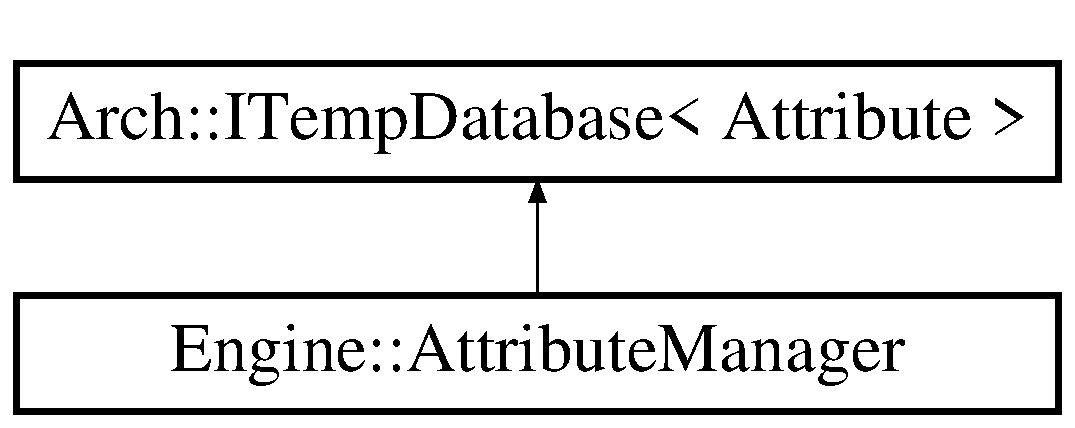
\includegraphics[height=2.000000cm]{classEngine_1_1AttributeManager}
\end{center}
\end{figure}
\subsection*{Public Member Functions}
\begin{DoxyCompactItemize}
\item 
\hyperlink{classEngine_1_1Attribute}{Attribute} $\ast$ \hyperlink{classEngine_1_1AttributeManager_af7dd02d47b84f2f33bd8dac19052fe40}{create\+Attribute} (const std\+::string \&attribute\+\_\+name)
\begin{DoxyCompactList}\small\item\em create\+Attribute \end{DoxyCompactList}\item 
\hyperlink{classEngine_1_1Attribute}{Attribute} $\ast$ \hyperlink{classEngine_1_1AttributeManager_a792f0247b709578ea95bc08810b943f4}{get\+Attribute} (uint component\+\_\+id)
\begin{DoxyCompactList}\small\item\em get\+Attribute \end{DoxyCompactList}\item 
void \hyperlink{classEngine_1_1AttributeManager_aded6608e85127ef6e1c3edd21e31fe36}{destroy} (uint component\+\_\+id)
\begin{DoxyCompactList}\small\item\em remove \end{DoxyCompactList}\end{DoxyCompactItemize}


\subsection{Detailed Description}
The \hyperlink{classEngine_1_1AttributeManager}{Attribute\+Manager} controlled Attributes. 

Componentv2 Database ( \hyperlink{classEngine_1_1AttributeManager}{Attribute\+Manager} ) 

\subsection{Member Function Documentation}
\hypertarget{classEngine_1_1AttributeManager_af7dd02d47b84f2f33bd8dac19052fe40}{}\index{Engine\+::\+Attribute\+Manager@{Engine\+::\+Attribute\+Manager}!create\+Attribute@{create\+Attribute}}
\index{create\+Attribute@{create\+Attribute}!Engine\+::\+Attribute\+Manager@{Engine\+::\+Attribute\+Manager}}
\subsubsection[{create\+Attribute(const std\+::string \&attribute\+\_\+name)}]{\setlength{\rightskip}{0pt plus 5cm}{\bf Attribute} $\ast$ Attribute\+Manager\+::create\+Attribute (
\begin{DoxyParamCaption}
\item[{const std\+::string \&}]{attribute\+\_\+name}
\end{DoxyParamCaption}
)}\label{classEngine_1_1AttributeManager_af7dd02d47b84f2f33bd8dac19052fe40}


create\+Attribute 

Create a new \hyperlink{classEngine_1_1Attribute}{Attribute} with name 
\begin{DoxyParams}{Parameters}
{\em attribute\+\_\+name} & \\
\hline
\end{DoxyParams}
\begin{DoxyReturn}{Returns}

\end{DoxyReturn}
\hypertarget{classEngine_1_1AttributeManager_aded6608e85127ef6e1c3edd21e31fe36}{}\index{Engine\+::\+Attribute\+Manager@{Engine\+::\+Attribute\+Manager}!destroy@{destroy}}
\index{destroy@{destroy}!Engine\+::\+Attribute\+Manager@{Engine\+::\+Attribute\+Manager}}
\subsubsection[{destroy(uint component\+\_\+id)}]{\setlength{\rightskip}{0pt plus 5cm}void Attribute\+Manager\+::destroy (
\begin{DoxyParamCaption}
\item[{uint}]{component\+\_\+id}
\end{DoxyParamCaption}
)}\label{classEngine_1_1AttributeManager_aded6608e85127ef6e1c3edd21e31fe36}


remove 

Remove \hyperlink{classEngine_1_1Attribute}{Attribute} 
\begin{DoxyParams}{Parameters}
{\em component\+\_\+id} & \\
\hline
\end{DoxyParams}
\hypertarget{classEngine_1_1AttributeManager_a792f0247b709578ea95bc08810b943f4}{}\index{Engine\+::\+Attribute\+Manager@{Engine\+::\+Attribute\+Manager}!get\+Attribute@{get\+Attribute}}
\index{get\+Attribute@{get\+Attribute}!Engine\+::\+Attribute\+Manager@{Engine\+::\+Attribute\+Manager}}
\subsubsection[{get\+Attribute(uint component\+\_\+id)}]{\setlength{\rightskip}{0pt plus 5cm}{\bf Attribute} $\ast$ Attribute\+Manager\+::get\+Attribute (
\begin{DoxyParamCaption}
\item[{uint}]{component\+\_\+id}
\end{DoxyParamCaption}
)}\label{classEngine_1_1AttributeManager_a792f0247b709578ea95bc08810b943f4}


get\+Attribute 

Return a \hyperlink{classEngine_1_1Attribute}{Attribute} by component\+\_\+id 
\begin{DoxyParams}{Parameters}
{\em component\+\_\+id} & \\
\hline
\end{DoxyParams}
\begin{DoxyReturn}{Returns}

\end{DoxyReturn}


The documentation for this class was generated from the following files\+:\begin{DoxyCompactItemize}
\item 
include/\+Manager/attributemanager.\+h\item 
Engine/\+Manager/Attribute\+Manager.\+cpp\end{DoxyCompactItemize}

\hypertarget{classEngine_1_1BasicColourTech}{}\section{Engine\+:\+:Basic\+Colour\+Tech Class Reference}
\label{classEngine_1_1BasicColourTech}\index{Engine\+::\+Basic\+Colour\+Tech@{Engine\+::\+Basic\+Colour\+Tech}}


The \hyperlink{classEngine_1_1BasicColourTech}{Basic\+Colour\+Tech} -\/ Basic \hyperlink{classEngine_1_1Technique}{Technique} class.  




{\ttfamily \#include $<$basiccolourtech.\+h$>$}

Inheritance diagram for Engine\+:\+:Basic\+Colour\+Tech\+:\begin{figure}[H]
\begin{center}
\leavevmode
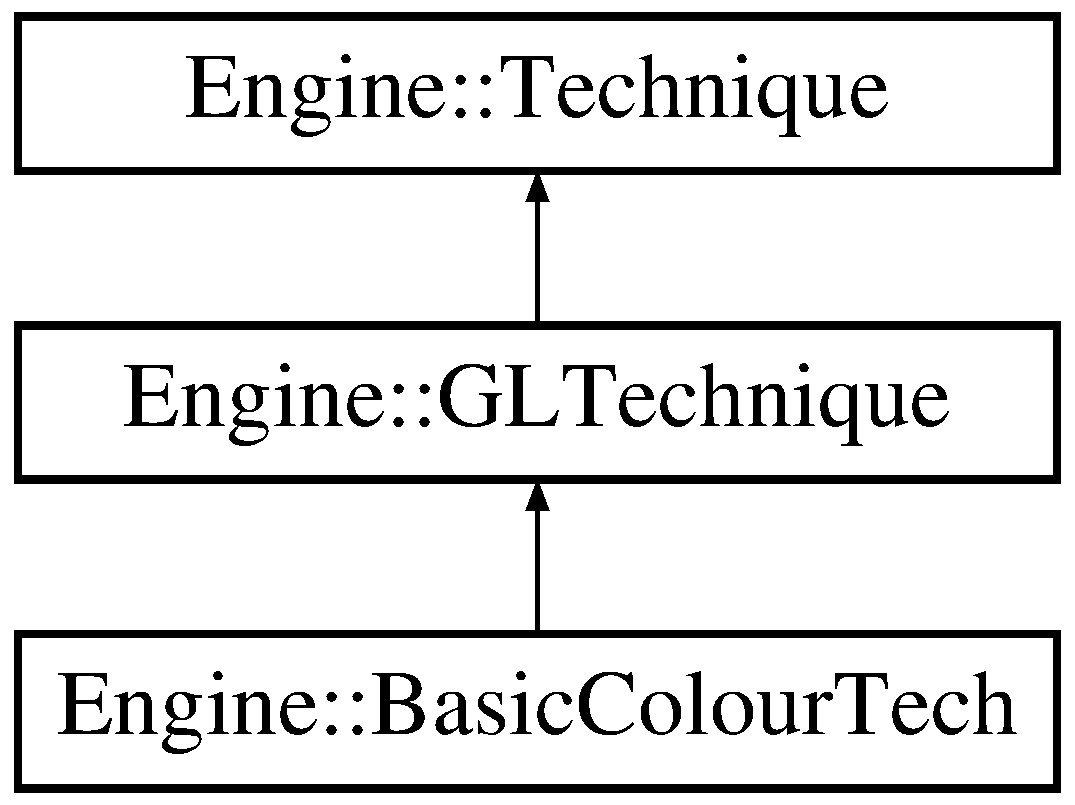
\includegraphics[height=3.000000cm]{classEngine_1_1BasicColourTech}
\end{center}
\end{figure}
\subsection*{Public Member Functions}
\begin{DoxyCompactItemize}
\item 
\hypertarget{classEngine_1_1BasicColourTech_aa6e9de1fc02b5e63ce95c94784090024}{}{\bfseries Basic\+Colour\+Tech} (const std\+::string \&name)\label{classEngine_1_1BasicColourTech_aa6e9de1fc02b5e63ce95c94784090024}

\item 
\hypertarget{classEngine_1_1BasicColourTech_a66ae830e78bdee64efe49b566da2f35e}{}void {\bfseries Create} (void)\label{classEngine_1_1BasicColourTech_a66ae830e78bdee64efe49b566da2f35e}

\item 
\hypertarget{classEngine_1_1BasicColourTech_adbabe9350d6d141703350e9870066b92}{}void {\bfseries Prepare} (void)\label{classEngine_1_1BasicColourTech_adbabe9350d6d141703350e9870066b92}

\item 
\hypertarget{classEngine_1_1BasicColourTech_a369eab1f7871a7b5045a33cca10e5c64}{}void {\bfseries Update} (void)\label{classEngine_1_1BasicColourTech_a369eab1f7871a7b5045a33cca10e5c64}

\item 
\hypertarget{classEngine_1_1BasicColourTech_a04d6c8a685d015645a121f41e4e99a6e}{}void {\bfseries Render} (\hyperlink{classEngine_1_1Texture}{Texture} $\ast$basic)\label{classEngine_1_1BasicColourTech_a04d6c8a685d015645a121f41e4e99a6e}

\end{DoxyCompactItemize}
\subsection*{Additional Inherited Members}


\subsection{Detailed Description}
The \hyperlink{classEngine_1_1BasicColourTech}{Basic\+Colour\+Tech} -\/ Basic \hyperlink{classEngine_1_1Technique}{Technique} class. 

The documentation for this class was generated from the following files\+:\begin{DoxyCompactItemize}
\item 
include/\+Technique/basiccolourtech.\+h\item 
Engine/\+Technique/Basic\+Colour\+Tech.\+cpp\end{DoxyCompactItemize}

\hypertarget{classEngine_1_1BasicRenderModul}{}\section{Engine\+:\+:Basic\+Render\+Modul Class Reference}
\label{classEngine_1_1BasicRenderModul}\index{Engine\+::\+Basic\+Render\+Modul@{Engine\+::\+Basic\+Render\+Modul}}
Inheritance diagram for Engine\+:\+:Basic\+Render\+Modul\+:\begin{figure}[H]
\begin{center}
\leavevmode
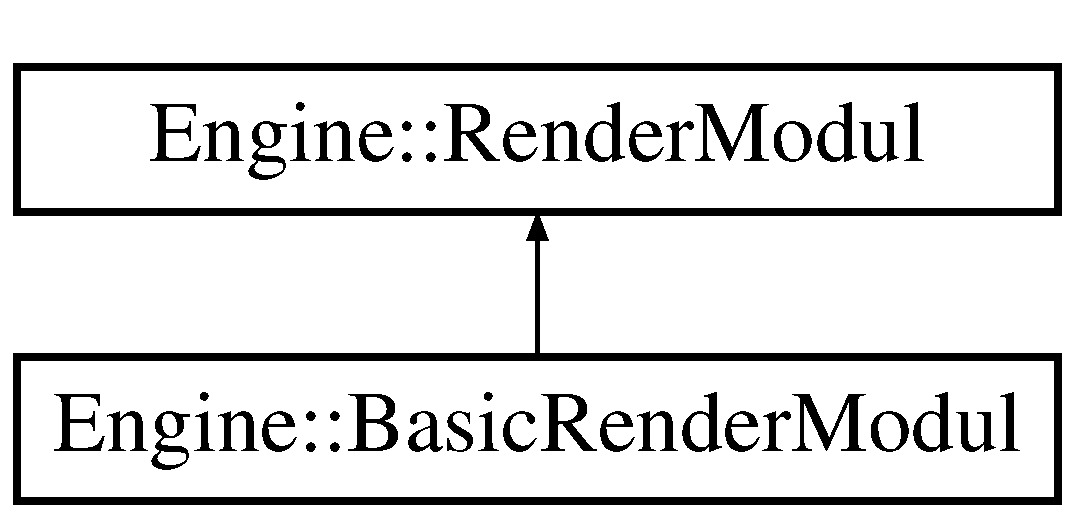
\includegraphics[height=2.000000cm]{classEngine_1_1BasicRenderModul}
\end{center}
\end{figure}
\subsection*{Public Member Functions}
\begin{DoxyCompactItemize}
\item 
\hypertarget{classEngine_1_1BasicRenderModul_a49ebb39a43cd4eb14061a1af93506f2f}{}void {\bfseries render\+Process} (const \hyperlink{classEngine_1_1DrawEvent}{Draw\+Event} \&event)\label{classEngine_1_1BasicRenderModul_a49ebb39a43cd4eb14061a1af93506f2f}

\end{DoxyCompactItemize}
\subsection*{Additional Inherited Members}


The documentation for this class was generated from the following files\+:\begin{DoxyCompactItemize}
\item 
include/\+Render/\+Modul/basicrendermodul.\+h\item 
Engine/\+Render/\+Modul/Basic\+Render\+Modul.\+cpp\end{DoxyCompactItemize}

\hypertarget{classEngine_1_1Bone}{}\section{Engine\+:\+:Bone Class Reference}
\label{classEngine_1_1Bone}\index{Engine\+::\+Bone@{Engine\+::\+Bone}}


The \hyperlink{classEngine_1_1Bone}{Bone} class.  




{\ttfamily \#include $<$bone.\+h$>$}

\subsection*{Public Member Functions}
\begin{DoxyCompactItemize}
\item 
\hypertarget{classEngine_1_1Bone_a43128067323ee8ca50b8b8ba20ff1d14}{}{\bfseries Bone} (const std\+::string \&bone\+\_\+name)\label{classEngine_1_1Bone_a43128067323ee8ca50b8b8ba20ff1d14}

\item 
void \hyperlink{classEngine_1_1Bone_a8cee234a0f0811bb0ec81266999c87ad}{set\+Parent} (\hyperlink{classEngine_1_1Bone}{Bone} $\ast$bone)
\begin{DoxyCompactList}\small\item\em set\+Parent \end{DoxyCompactList}\item 
void \hyperlink{classEngine_1_1Bone_ad67ca7e8863ae1207a6bbc7b1fb7dcba}{set\+Name} (const std\+::string \&bone\+\_\+name)
\begin{DoxyCompactList}\small\item\em set\+Name \end{DoxyCompactList}\item 
void \hyperlink{classEngine_1_1Bone_a6e1880832768227605594b922bd8cd7d}{set\+Offset\+Position} (const \hyperlink{classVector3}{Vector3f} \&position)
\begin{DoxyCompactList}\small\item\em set\+Offset\+Position \end{DoxyCompactList}\item 
\hypertarget{classEngine_1_1Bone_aa9fa7c60c56aafcf4574c2cad701d2f8}{}void {\bfseries set\+Offset} (const \hyperlink{classVector3}{Vector3f} \&position)\label{classEngine_1_1Bone_aa9fa7c60c56aafcf4574c2cad701d2f8}

\item 
void \hyperlink{classEngine_1_1Bone_a31f669188801946033a4cd2704253028}{set\+Key\+Frames} (Key\+Frames frames)
\begin{DoxyCompactList}\small\item\em set\+Key\+Frames \end{DoxyCompactList}\item 
void \hyperlink{classEngine_1_1Bone_a54e2cf46c426ab8fa787e4f1cc27829d}{set\+Vertex\+Group} (\hyperlink{classEngine_1_1VertexGroup}{Vertex\+Group} $\ast$group)
\begin{DoxyCompactList}\small\item\em set\+Vertex\+Group \end{DoxyCompactList}\item 
void \hyperlink{classEngine_1_1Bone_a710598e6b40ae08fa8b5e14b1e010351}{add\+Key\+Frame} (\hyperlink{classEngine_1_1KeyFrame}{Key\+Frame} $\ast$frame)
\begin{DoxyCompactList}\small\item\em add\+Key\+Frame \end{DoxyCompactList}\item 
const std\+::string \& \hyperlink{classEngine_1_1Bone_a6f332bea5d510644687ccfec8604350c}{get\+Name} (void) const 
\begin{DoxyCompactList}\small\item\em get\+Name \end{DoxyCompactList}\item 
const \hyperlink{classVector3}{Vector3f} \& \hyperlink{classEngine_1_1Bone_a55e9791c1f09e1b0ef6f18662dbc3351}{get\+Position} (void) const 
\begin{DoxyCompactList}\small\item\em get\+Position \end{DoxyCompactList}\item 
const \hyperlink{classVector3}{Vector3f} \& \hyperlink{classEngine_1_1Bone_a60208f0fa2aa5853df588316c2f9f86d}{get\+Offset} (void)
\begin{DoxyCompactList}\small\item\em get\+Offset \end{DoxyCompactList}\item 
Key\+Frames \hyperlink{classEngine_1_1Bone_a8470ce520de7caa512a3198f7756b95e}{get\+Frames} (void) const 
\begin{DoxyCompactList}\small\item\em get\+Frames \end{DoxyCompactList}\item 
\hyperlink{classEngine_1_1VertexGroup}{Vertex\+Group} $\ast$ \hyperlink{classEngine_1_1Bone_af5724489766e3fc6505d41812131bf53}{get\+Vertex\+Group} (void) const 
\begin{DoxyCompactList}\small\item\em get\+Vertex\+Group \end{DoxyCompactList}\item 
\hyperlink{classEngine_1_1Bone}{Bone} $\ast$ \hyperlink{classEngine_1_1Bone_a1e1988b7d346df3c2f918a1455aa8361}{get\+Parent} (void)
\begin{DoxyCompactList}\small\item\em get\+Parent \end{DoxyCompactList}\end{DoxyCompactItemize}


\subsection{Detailed Description}
The \hyperlink{classEngine_1_1Bone}{Bone} class. 

Save \hyperlink{classEngine_1_1Bone}{Bone} Data 

\subsection{Member Function Documentation}
\hypertarget{classEngine_1_1Bone_a710598e6b40ae08fa8b5e14b1e010351}{}\index{Engine\+::\+Bone@{Engine\+::\+Bone}!add\+Key\+Frame@{add\+Key\+Frame}}
\index{add\+Key\+Frame@{add\+Key\+Frame}!Engine\+::\+Bone@{Engine\+::\+Bone}}
\subsubsection[{add\+Key\+Frame(\+Key\+Frame $\ast$frame)}]{\setlength{\rightskip}{0pt plus 5cm}void Bone\+::add\+Key\+Frame (
\begin{DoxyParamCaption}
\item[{{\bf Key\+Frame} $\ast$}]{frame}
\end{DoxyParamCaption}
)}\label{classEngine_1_1Bone_a710598e6b40ae08fa8b5e14b1e010351}


add\+Key\+Frame 

Add a \hyperlink{classEngine_1_1KeyFrame}{Key\+Frame} 
\begin{DoxyParams}{Parameters}
{\em frame} & \\
\hline
\end{DoxyParams}
\hypertarget{classEngine_1_1Bone_a8470ce520de7caa512a3198f7756b95e}{}\index{Engine\+::\+Bone@{Engine\+::\+Bone}!get\+Frames@{get\+Frames}}
\index{get\+Frames@{get\+Frames}!Engine\+::\+Bone@{Engine\+::\+Bone}}
\subsubsection[{get\+Frames(void) const }]{\setlength{\rightskip}{0pt plus 5cm}Key\+Frames Bone\+::get\+Frames (
\begin{DoxyParamCaption}
\item[{void}]{}
\end{DoxyParamCaption}
) const}\label{classEngine_1_1Bone_a8470ce520de7caa512a3198f7756b95e}


get\+Frames 

Return all Key\+Frames \begin{DoxyReturn}{Returns}

\end{DoxyReturn}
\hypertarget{classEngine_1_1Bone_a6f332bea5d510644687ccfec8604350c}{}\index{Engine\+::\+Bone@{Engine\+::\+Bone}!get\+Name@{get\+Name}}
\index{get\+Name@{get\+Name}!Engine\+::\+Bone@{Engine\+::\+Bone}}
\subsubsection[{get\+Name(void) const }]{\setlength{\rightskip}{0pt plus 5cm}const std\+::string \& Bone\+::get\+Name (
\begin{DoxyParamCaption}
\item[{void}]{}
\end{DoxyParamCaption}
) const}\label{classEngine_1_1Bone_a6f332bea5d510644687ccfec8604350c}


get\+Name 

Return \hyperlink{classEngine_1_1Bone}{Bone} Name \begin{DoxyReturn}{Returns}

\end{DoxyReturn}
\hypertarget{classEngine_1_1Bone_a60208f0fa2aa5853df588316c2f9f86d}{}\index{Engine\+::\+Bone@{Engine\+::\+Bone}!get\+Offset@{get\+Offset}}
\index{get\+Offset@{get\+Offset}!Engine\+::\+Bone@{Engine\+::\+Bone}}
\subsubsection[{get\+Offset(void)}]{\setlength{\rightskip}{0pt plus 5cm}const {\bf Vector3f} \& Bone\+::get\+Offset (
\begin{DoxyParamCaption}
\item[{void}]{}
\end{DoxyParamCaption}
)}\label{classEngine_1_1Bone_a60208f0fa2aa5853df588316c2f9f86d}


get\+Offset 

Return (.rel) \hyperlink{classEngine_1_1Position}{Position} \begin{DoxyReturn}{Returns}

\end{DoxyReturn}
\hypertarget{classEngine_1_1Bone_a1e1988b7d346df3c2f918a1455aa8361}{}\index{Engine\+::\+Bone@{Engine\+::\+Bone}!get\+Parent@{get\+Parent}}
\index{get\+Parent@{get\+Parent}!Engine\+::\+Bone@{Engine\+::\+Bone}}
\subsubsection[{get\+Parent(void)}]{\setlength{\rightskip}{0pt plus 5cm}{\bf Bone} $\ast$ Bone\+::get\+Parent (
\begin{DoxyParamCaption}
\item[{void}]{}
\end{DoxyParamCaption}
)}\label{classEngine_1_1Bone_a1e1988b7d346df3c2f918a1455aa8361}


get\+Parent 

Return parent \hyperlink{classEngine_1_1Bone}{Bone} \begin{DoxyReturn}{Returns}

\end{DoxyReturn}
\hypertarget{classEngine_1_1Bone_a55e9791c1f09e1b0ef6f18662dbc3351}{}\index{Engine\+::\+Bone@{Engine\+::\+Bone}!get\+Position@{get\+Position}}
\index{get\+Position@{get\+Position}!Engine\+::\+Bone@{Engine\+::\+Bone}}
\subsubsection[{get\+Position(void) const }]{\setlength{\rightskip}{0pt plus 5cm}const {\bf Vector3f} \& Bone\+::get\+Position (
\begin{DoxyParamCaption}
\item[{void}]{}
\end{DoxyParamCaption}
) const}\label{classEngine_1_1Bone_a55e9791c1f09e1b0ef6f18662dbc3351}


get\+Position 

Return (.abs) \hyperlink{classEngine_1_1Position}{Position} \begin{DoxyReturn}{Returns}

\end{DoxyReturn}
\hypertarget{classEngine_1_1Bone_af5724489766e3fc6505d41812131bf53}{}\index{Engine\+::\+Bone@{Engine\+::\+Bone}!get\+Vertex\+Group@{get\+Vertex\+Group}}
\index{get\+Vertex\+Group@{get\+Vertex\+Group}!Engine\+::\+Bone@{Engine\+::\+Bone}}
\subsubsection[{get\+Vertex\+Group(void) const }]{\setlength{\rightskip}{0pt plus 5cm}{\bf Vertex\+Group} $\ast$ Bone\+::get\+Vertex\+Group (
\begin{DoxyParamCaption}
\item[{void}]{}
\end{DoxyParamCaption}
) const}\label{classEngine_1_1Bone_af5724489766e3fc6505d41812131bf53}


get\+Vertex\+Group 

Return \hyperlink{classEngine_1_1VertexGroup}{Vertex\+Group} \begin{DoxyReturn}{Returns}

\end{DoxyReturn}
\hypertarget{classEngine_1_1Bone_a31f669188801946033a4cd2704253028}{}\index{Engine\+::\+Bone@{Engine\+::\+Bone}!set\+Key\+Frames@{set\+Key\+Frames}}
\index{set\+Key\+Frames@{set\+Key\+Frames}!Engine\+::\+Bone@{Engine\+::\+Bone}}
\subsubsection[{set\+Key\+Frames(\+Key\+Frames frames)}]{\setlength{\rightskip}{0pt plus 5cm}void Bone\+::set\+Key\+Frames (
\begin{DoxyParamCaption}
\item[{Key\+Frames}]{frames}
\end{DoxyParamCaption}
)}\label{classEngine_1_1Bone_a31f669188801946033a4cd2704253028}


set\+Key\+Frames 

set Key\+Frames 
\begin{DoxyParams}{Parameters}
{\em frames} & \\
\hline
\end{DoxyParams}
\hypertarget{classEngine_1_1Bone_ad67ca7e8863ae1207a6bbc7b1fb7dcba}{}\index{Engine\+::\+Bone@{Engine\+::\+Bone}!set\+Name@{set\+Name}}
\index{set\+Name@{set\+Name}!Engine\+::\+Bone@{Engine\+::\+Bone}}
\subsubsection[{set\+Name(const std\+::string \&bone\+\_\+name)}]{\setlength{\rightskip}{0pt plus 5cm}void Bone\+::set\+Name (
\begin{DoxyParamCaption}
\item[{const std\+::string \&}]{bone\+\_\+name}
\end{DoxyParamCaption}
)}\label{classEngine_1_1Bone_ad67ca7e8863ae1207a6bbc7b1fb7dcba}


set\+Name 

Set \hyperlink{classEngine_1_1Bone}{Bone} Name 
\begin{DoxyParams}{Parameters}
{\em bone\+\_\+name} & \\
\hline
\end{DoxyParams}
\hypertarget{classEngine_1_1Bone_a6e1880832768227605594b922bd8cd7d}{}\index{Engine\+::\+Bone@{Engine\+::\+Bone}!set\+Offset\+Position@{set\+Offset\+Position}}
\index{set\+Offset\+Position@{set\+Offset\+Position}!Engine\+::\+Bone@{Engine\+::\+Bone}}
\subsubsection[{set\+Offset\+Position(const Vector3f \&position)}]{\setlength{\rightskip}{0pt plus 5cm}void Bone\+::set\+Offset\+Position (
\begin{DoxyParamCaption}
\item[{const {\bf Vector3f} \&}]{position}
\end{DoxyParamCaption}
)}\label{classEngine_1_1Bone_a6e1880832768227605594b922bd8cd7d}


set\+Offset\+Position 

set Offset \hyperlink{classEngine_1_1Position}{Position} ( abs.) 
\begin{DoxyParams}{Parameters}
{\em position} & \\
\hline
\end{DoxyParams}
\hypertarget{classEngine_1_1Bone_a8cee234a0f0811bb0ec81266999c87ad}{}\index{Engine\+::\+Bone@{Engine\+::\+Bone}!set\+Parent@{set\+Parent}}
\index{set\+Parent@{set\+Parent}!Engine\+::\+Bone@{Engine\+::\+Bone}}
\subsubsection[{set\+Parent(\+Bone $\ast$bone)}]{\setlength{\rightskip}{0pt plus 5cm}void Bone\+::set\+Parent (
\begin{DoxyParamCaption}
\item[{{\bf Bone} $\ast$}]{bone}
\end{DoxyParamCaption}
)}\label{classEngine_1_1Bone_a8cee234a0f0811bb0ec81266999c87ad}


set\+Parent 

Set parent \hyperlink{classEngine_1_1Bone}{Bone} 
\begin{DoxyParams}{Parameters}
{\em bone} & \\
\hline
\end{DoxyParams}
\hypertarget{classEngine_1_1Bone_a54e2cf46c426ab8fa787e4f1cc27829d}{}\index{Engine\+::\+Bone@{Engine\+::\+Bone}!set\+Vertex\+Group@{set\+Vertex\+Group}}
\index{set\+Vertex\+Group@{set\+Vertex\+Group}!Engine\+::\+Bone@{Engine\+::\+Bone}}
\subsubsection[{set\+Vertex\+Group(\+Vertex\+Group $\ast$group)}]{\setlength{\rightskip}{0pt plus 5cm}void Bone\+::set\+Vertex\+Group (
\begin{DoxyParamCaption}
\item[{{\bf Vertex\+Group} $\ast$}]{group}
\end{DoxyParamCaption}
)}\label{classEngine_1_1Bone_a54e2cf46c426ab8fa787e4f1cc27829d}


set\+Vertex\+Group 

set \hyperlink{classEngine_1_1VertexGroup}{Vertex\+Group} 
\begin{DoxyParams}{Parameters}
{\em group} & \\
\hline
\end{DoxyParams}


The documentation for this class was generated from the following files\+:\begin{DoxyCompactItemize}
\item 
include/\+Container/bone.\+h\item 
Container/Bone.\+cpp\end{DoxyCompactItemize}

\hypertarget{classEngine_1_1BvhLoader}{}\section{Engine\+:\+:Bvh\+Loader Class Reference}
\label{classEngine_1_1BvhLoader}\index{Engine\+::\+Bvh\+Loader@{Engine\+::\+Bvh\+Loader}}


The \hyperlink{classEngine_1_1BvhLoader}{Bvh\+Loader} -\/ B\+V\+H File Loader ( .bvh )  




{\ttfamily \#include $<$bvhloader.\+h$>$}

Inheritance diagram for Engine\+:\+:Bvh\+Loader\+:\begin{figure}[H]
\begin{center}
\leavevmode
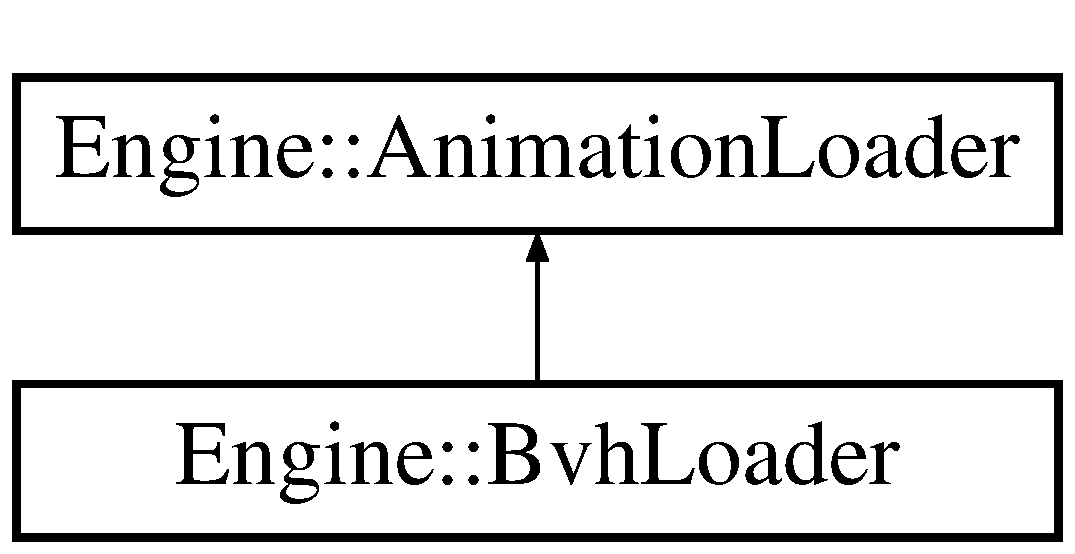
\includegraphics[height=2.000000cm]{classEngine_1_1BvhLoader}
\end{center}
\end{figure}
\subsection*{Classes}
\begin{DoxyCompactItemize}
\item 
struct \hyperlink{structEngine_1_1BvhLoader_1_1StoreState}{Store\+State}
\begin{DoxyCompactList}\small\item\em The \hyperlink{structEngine_1_1BvhLoader_1_1StoreState}{Store\+State} struct. \end{DoxyCompactList}\end{DoxyCompactItemize}
\subsection*{Public Types}
\begin{DoxyCompactItemize}
\item 
\hypertarget{classEngine_1_1BvhLoader_aec0215c1beb225aee94b6f57ad13adaf}{}using {\bfseries H\+M\+State\+Store} = struct \hyperlink{structEngine_1_1BvhLoader_1_1StoreState}{Store\+State}\label{classEngine_1_1BvhLoader_aec0215c1beb225aee94b6f57ad13adaf}

\end{DoxyCompactItemize}
\subsection*{Public Member Functions}
\begin{DoxyCompactItemize}
\item 
\hyperlink{classEngine_1_1BvhLoader_a6ce825c92ae428a0366410eab5d990aa}{Bvh\+Loader} ()
\begin{DoxyCompactList}\small\item\em \hyperlink{classEngine_1_1BvhLoader}{Bvh\+Loader}. \end{DoxyCompactList}\item 
void \hyperlink{classEngine_1_1BvhLoader_abd58f0b7f498fcb4f25bfe7f15a310d4}{Read\+File} (const string \&motion\+\_\+file, \hyperlink{classEngine_1_1NodeAnimScene}{Node\+Anim\+Scene} $\ast$node\+\_\+anim\+\_\+scene)
\begin{DoxyCompactList}\small\item\em Read\+File. \end{DoxyCompactList}\item 
void \hyperlink{classEngine_1_1BvhLoader_a599ca8a71e770128f27769e13f12aa63}{Read\+Hierachy} (\hyperlink{classEngine_1_1NodeAnimScene}{Node\+Anim\+Scene} $\ast$node\+\_\+anim\+\_\+scene)
\begin{DoxyCompactList}\small\item\em Read\+Hierachy. \end{DoxyCompactList}\item 
void \hyperlink{classEngine_1_1BvhLoader_ac22c70132e353ef1a91135911e8c1382}{Read\+Motion} (\hyperlink{classEngine_1_1NodeAnimScene}{Node\+Anim\+Scene} $\ast$node\+\_\+anim\+\_\+scene)
\begin{DoxyCompactList}\small\item\em Read\+Motion. \end{DoxyCompactList}\item 
void \hyperlink{classEngine_1_1BvhLoader_af97fd5b3c463a2d7cb83b091173a2d2e}{prepare\+By\+Flags} (\hyperlink{classEngine_1_1NodeAnimScene}{Node\+Anim\+Scene} $\ast$node\+\_\+anim\+\_\+scene)
\begin{DoxyCompactList}\small\item\em prepare\+By\+Flags \end{DoxyCompactList}\item 
void \hyperlink{classEngine_1_1BvhLoader_a4840a1a13d575617171caa923de7a494}{bvh\+\_\+string\+\_\+split} (const std\+::string \&line, char delim, Strings \&items)
\begin{DoxyCompactList}\small\item\em bvh\+\_\+string\+\_\+split \end{DoxyCompactList}\item 
std\+::string \hyperlink{classEngine_1_1BvhLoader_a7130a9d03688b504b3b6bbe27010ddad}{get\+Node\+Name} (const std\+::string \&line)
\begin{DoxyCompactList}\small\item\em get\+Node\+Name \end{DoxyCompactList}\item 
std\+::string \hyperlink{classEngine_1_1BvhLoader_afefebc57a1204d9244b097664e223f35}{get\+First} (const std\+::string \&line)
\begin{DoxyCompactList}\small\item\em get\+First \end{DoxyCompactList}\item 
\hyperlink{classVector3}{Vector3f} \hyperlink{classEngine_1_1BvhLoader_a9a79af2338a7c428076b212823d3d714}{get\+Offset} (const std\+::string \&line)
\begin{DoxyCompactList}\small\item\em get\+Offset \end{DoxyCompactList}\item 
int \hyperlink{classEngine_1_1BvhLoader_a8704cf6e1c413be669d2322ee8db9fb5}{get\+Frames} (const std\+::string \&line)
\begin{DoxyCompactList}\small\item\em get\+Frames \end{DoxyCompactList}\item 
\hyperlink{classEngine_1_1NodeAnim}{Node\+Anim} $\ast$ \hyperlink{classEngine_1_1BvhLoader_ad4528687a88e9e6fceff3d8de2f571a2}{get\+Node} (const \hyperlink{classVector3}{Vector3f} \&offset, \hyperlink{classEngine_1_1NodeAnimScene}{Node\+Anim\+Scene} $\ast$scene)
\begin{DoxyCompactList}\small\item\em get\+Node \end{DoxyCompactList}\item 
void \hyperlink{classEngine_1_1BvhLoader_af328fc4f00cb017298b5a979f27a0f63}{Print\+Error} (const \hyperlink{classVector3}{Vector3f} \&offset)  throw ( std\+::runtime\+\_\+error )
\begin{DoxyCompactList}\small\item\em Print\+Error. \end{DoxyCompactList}\item 
float \hyperlink{classEngine_1_1BvhLoader_a57670cf4d7d33cf1f45c6643f940b271}{get\+Number} (const std\+::string \&item)
\end{DoxyCompactItemize}
\subsection*{Additional Inherited Members}


\subsection{Detailed Description}
The \hyperlink{classEngine_1_1BvhLoader}{Bvh\+Loader} -\/ B\+V\+H File Loader ( .bvh ) 

\subsection{Constructor \& Destructor Documentation}
\hypertarget{classEngine_1_1BvhLoader_a6ce825c92ae428a0366410eab5d990aa}{}\index{Engine\+::\+Bvh\+Loader@{Engine\+::\+Bvh\+Loader}!Bvh\+Loader@{Bvh\+Loader}}
\index{Bvh\+Loader@{Bvh\+Loader}!Engine\+::\+Bvh\+Loader@{Engine\+::\+Bvh\+Loader}}
\subsubsection[{Bvh\+Loader()}]{\setlength{\rightskip}{0pt plus 5cm}Bvh\+Loader\+::\+Bvh\+Loader (
\begin{DoxyParamCaption}
{}
\end{DoxyParamCaption}
)}\label{classEngine_1_1BvhLoader_a6ce825c92ae428a0366410eab5d990aa}


\hyperlink{classEngine_1_1BvhLoader}{Bvh\+Loader}. 

Default Constructor 

\subsection{Member Function Documentation}
\hypertarget{classEngine_1_1BvhLoader_a4840a1a13d575617171caa923de7a494}{}\index{Engine\+::\+Bvh\+Loader@{Engine\+::\+Bvh\+Loader}!bvh\+\_\+string\+\_\+split@{bvh\+\_\+string\+\_\+split}}
\index{bvh\+\_\+string\+\_\+split@{bvh\+\_\+string\+\_\+split}!Engine\+::\+Bvh\+Loader@{Engine\+::\+Bvh\+Loader}}
\subsubsection[{bvh\+\_\+string\+\_\+split(const std\+::string \&line, char delim, Strings \&items)}]{\setlength{\rightskip}{0pt plus 5cm}void Bvh\+Loader\+::bvh\+\_\+string\+\_\+split (
\begin{DoxyParamCaption}
\item[{const std\+::string \&}]{line, }
\item[{char}]{delim, }
\item[{Strings \&}]{items}
\end{DoxyParamCaption}
)}\label{classEngine_1_1BvhLoader_a4840a1a13d575617171caa923de7a494}


bvh\+\_\+string\+\_\+split 


\begin{DoxyParams}{Parameters}
{\em line} & \\
\hline
{\em delim} & \\
\hline
{\em items} & \\
\hline
\end{DoxyParams}
\hypertarget{classEngine_1_1BvhLoader_afefebc57a1204d9244b097664e223f35}{}\index{Engine\+::\+Bvh\+Loader@{Engine\+::\+Bvh\+Loader}!get\+First@{get\+First}}
\index{get\+First@{get\+First}!Engine\+::\+Bvh\+Loader@{Engine\+::\+Bvh\+Loader}}
\subsubsection[{get\+First(const std\+::string \&line)}]{\setlength{\rightskip}{0pt plus 5cm}std\+::string Bvh\+Loader\+::get\+First (
\begin{DoxyParamCaption}
\item[{const std\+::string \&}]{line}
\end{DoxyParamCaption}
)}\label{classEngine_1_1BvhLoader_afefebc57a1204d9244b097664e223f35}


get\+First 

Return first \hyperlink{classEngine_1_1Element}{Element} from current line 
\begin{DoxyParams}{Parameters}
{\em line} & \\
\hline
\end{DoxyParams}
\begin{DoxyReturn}{Returns}

\end{DoxyReturn}
\hypertarget{classEngine_1_1BvhLoader_a8704cf6e1c413be669d2322ee8db9fb5}{}\index{Engine\+::\+Bvh\+Loader@{Engine\+::\+Bvh\+Loader}!get\+Frames@{get\+Frames}}
\index{get\+Frames@{get\+Frames}!Engine\+::\+Bvh\+Loader@{Engine\+::\+Bvh\+Loader}}
\subsubsection[{get\+Frames(const std\+::string \&line)}]{\setlength{\rightskip}{0pt plus 5cm}int Bvh\+Loader\+::get\+Frames (
\begin{DoxyParamCaption}
\item[{const std\+::string \&}]{line}
\end{DoxyParamCaption}
)}\label{classEngine_1_1BvhLoader_a8704cf6e1c413be669d2322ee8db9fb5}


get\+Frames 

Return max. frames from current line 
\begin{DoxyParams}{Parameters}
{\em line} & \\
\hline
\end{DoxyParams}
\begin{DoxyReturn}{Returns}

\end{DoxyReturn}
\hypertarget{classEngine_1_1BvhLoader_ad4528687a88e9e6fceff3d8de2f571a2}{}\index{Engine\+::\+Bvh\+Loader@{Engine\+::\+Bvh\+Loader}!get\+Node@{get\+Node}}
\index{get\+Node@{get\+Node}!Engine\+::\+Bvh\+Loader@{Engine\+::\+Bvh\+Loader}}
\subsubsection[{get\+Node(const Vector3f \&offset, Node\+Anim\+Scene $\ast$scene)}]{\setlength{\rightskip}{0pt plus 5cm}{\bf Node\+Anim} $\ast$ Bvh\+Loader\+::get\+Node (
\begin{DoxyParamCaption}
\item[{const {\bf Vector3f} \&}]{offset, }
\item[{{\bf Node\+Anim\+Scene} $\ast$}]{scene}
\end{DoxyParamCaption}
)}\label{classEngine_1_1BvhLoader_ad4528687a88e9e6fceff3d8de2f571a2}


get\+Node 

Return Node by offset position from \hyperlink{classEngine_1_1NodeAnimScene}{Node\+Anim\+Scene} 
\begin{DoxyParams}{Parameters}
{\em offset} & \\
\hline
{\em scene} & \\
\hline
\end{DoxyParams}
\begin{DoxyReturn}{Returns}

\end{DoxyReturn}
\hypertarget{classEngine_1_1BvhLoader_a7130a9d03688b504b3b6bbe27010ddad}{}\index{Engine\+::\+Bvh\+Loader@{Engine\+::\+Bvh\+Loader}!get\+Node\+Name@{get\+Node\+Name}}
\index{get\+Node\+Name@{get\+Node\+Name}!Engine\+::\+Bvh\+Loader@{Engine\+::\+Bvh\+Loader}}
\subsubsection[{get\+Node\+Name(const std\+::string \&line)}]{\setlength{\rightskip}{0pt plus 5cm}std\+::string Bvh\+Loader\+::get\+Node\+Name (
\begin{DoxyParamCaption}
\item[{const std\+::string \&}]{line}
\end{DoxyParamCaption}
)}\label{classEngine_1_1BvhLoader_a7130a9d03688b504b3b6bbe27010ddad}


get\+Node\+Name 

Return Node\+Name from current line 
\begin{DoxyParams}{Parameters}
{\em line} & \\
\hline
\end{DoxyParams}
\begin{DoxyReturn}{Returns}

\end{DoxyReturn}
\hypertarget{classEngine_1_1BvhLoader_a57670cf4d7d33cf1f45c6643f940b271}{}\index{Engine\+::\+Bvh\+Loader@{Engine\+::\+Bvh\+Loader}!get\+Number@{get\+Number}}
\index{get\+Number@{get\+Number}!Engine\+::\+Bvh\+Loader@{Engine\+::\+Bvh\+Loader}}
\subsubsection[{get\+Number(const std\+::string \&item)}]{\setlength{\rightskip}{0pt plus 5cm}float Bvh\+Loader\+::get\+Number (
\begin{DoxyParamCaption}
\item[{const std\+::string \&}]{item}
\end{DoxyParamCaption}
)}\label{classEngine_1_1BvhLoader_a57670cf4d7d33cf1f45c6643f940b271}

\begin{DoxyParams}{Parameters}
{\em item} & \\
\hline
\end{DoxyParams}
\begin{DoxyReturn}{Returns}
float 
\end{DoxyReturn}
\hypertarget{classEngine_1_1BvhLoader_a9a79af2338a7c428076b212823d3d714}{}\index{Engine\+::\+Bvh\+Loader@{Engine\+::\+Bvh\+Loader}!get\+Offset@{get\+Offset}}
\index{get\+Offset@{get\+Offset}!Engine\+::\+Bvh\+Loader@{Engine\+::\+Bvh\+Loader}}
\subsubsection[{get\+Offset(const std\+::string \&line)}]{\setlength{\rightskip}{0pt plus 5cm}{\bf Vector3f} Bvh\+Loader\+::get\+Offset (
\begin{DoxyParamCaption}
\item[{const std\+::string \&}]{line}
\end{DoxyParamCaption}
)}\label{classEngine_1_1BvhLoader_a9a79af2338a7c428076b212823d3d714}


get\+Offset 

Return Offset \hyperlink{classEngine_1_1Position}{Position} from current line 
\begin{DoxyParams}{Parameters}
{\em line} & \\
\hline
\end{DoxyParams}
\begin{DoxyReturn}{Returns}

\end{DoxyReturn}
\hypertarget{classEngine_1_1BvhLoader_af97fd5b3c463a2d7cb83b091173a2d2e}{}\index{Engine\+::\+Bvh\+Loader@{Engine\+::\+Bvh\+Loader}!prepare\+By\+Flags@{prepare\+By\+Flags}}
\index{prepare\+By\+Flags@{prepare\+By\+Flags}!Engine\+::\+Bvh\+Loader@{Engine\+::\+Bvh\+Loader}}
\subsubsection[{prepare\+By\+Flags(\+Node\+Anim\+Scene $\ast$node\+\_\+anim\+\_\+scene)}]{\setlength{\rightskip}{0pt plus 5cm}void Bvh\+Loader\+::prepare\+By\+Flags (
\begin{DoxyParamCaption}
\item[{{\bf Node\+Anim\+Scene} $\ast$}]{node\+\_\+anim\+\_\+scene}
\end{DoxyParamCaption}
)}\label{classEngine_1_1BvhLoader_af97fd5b3c463a2d7cb83b091173a2d2e}


prepare\+By\+Flags 

Modifier anim scene by flags 
\begin{DoxyParams}{Parameters}
{\em node\+\_\+anim\+\_\+scene} & \\
\hline
\end{DoxyParams}
Information\+: Blender Z Negative is Open\+G\+L Y Positive\hypertarget{classEngine_1_1BvhLoader_af328fc4f00cb017298b5a979f27a0f63}{}\index{Engine\+::\+Bvh\+Loader@{Engine\+::\+Bvh\+Loader}!Print\+Error@{Print\+Error}}
\index{Print\+Error@{Print\+Error}!Engine\+::\+Bvh\+Loader@{Engine\+::\+Bvh\+Loader}}
\subsubsection[{Print\+Error(const Vector3f \&offset)}]{\setlength{\rightskip}{0pt plus 5cm}void Bvh\+Loader\+::\+Print\+Error (
\begin{DoxyParamCaption}
\item[{const {\bf Vector3f} \&}]{offset}
\end{DoxyParamCaption}
) throw  std\+::runtime\+\_\+error) }\label{classEngine_1_1BvhLoader_af328fc4f00cb017298b5a979f27a0f63}


Print\+Error. 


\begin{DoxyParams}{Parameters}
{\em offset} & \\
\hline
\end{DoxyParams}
\hypertarget{classEngine_1_1BvhLoader_abd58f0b7f498fcb4f25bfe7f15a310d4}{}\index{Engine\+::\+Bvh\+Loader@{Engine\+::\+Bvh\+Loader}!Read\+File@{Read\+File}}
\index{Read\+File@{Read\+File}!Engine\+::\+Bvh\+Loader@{Engine\+::\+Bvh\+Loader}}
\subsubsection[{Read\+File(const string \&motion\+\_\+file, Node\+Anim\+Scene $\ast$node\+\_\+anim\+\_\+scene)}]{\setlength{\rightskip}{0pt plus 5cm}void Bvh\+Loader\+::\+Read\+File (
\begin{DoxyParamCaption}
\item[{const string \&}]{motion\+\_\+file, }
\item[{{\bf Node\+Anim\+Scene} $\ast$}]{node\+\_\+anim\+\_\+scene}
\end{DoxyParamCaption}
)}\label{classEngine_1_1BvhLoader_abd58f0b7f498fcb4f25bfe7f15a310d4}


Read\+File. 

Read B\+V\+H File 
\begin{DoxyParams}{Parameters}
{\em motion\+\_\+file} & \\
\hline
{\em node\+\_\+anim\+\_\+scene} & \\
\hline
\end{DoxyParams}
\hypertarget{classEngine_1_1BvhLoader_a599ca8a71e770128f27769e13f12aa63}{}\index{Engine\+::\+Bvh\+Loader@{Engine\+::\+Bvh\+Loader}!Read\+Hierachy@{Read\+Hierachy}}
\index{Read\+Hierachy@{Read\+Hierachy}!Engine\+::\+Bvh\+Loader@{Engine\+::\+Bvh\+Loader}}
\subsubsection[{Read\+Hierachy(\+Node\+Anim\+Scene $\ast$node\+\_\+anim\+\_\+scene)}]{\setlength{\rightskip}{0pt plus 5cm}void Bvh\+Loader\+::\+Read\+Hierachy (
\begin{DoxyParamCaption}
\item[{{\bf Node\+Anim\+Scene} $\ast$}]{node\+\_\+anim\+\_\+scene}
\end{DoxyParamCaption}
)}\label{classEngine_1_1BvhLoader_a599ca8a71e770128f27769e13f12aa63}


Read\+Hierachy. 

Read Hierachy Part and save data into node\+\_\+anim\+\_\+scene 
\begin{DoxyParams}{Parameters}
{\em node\+\_\+anim\+\_\+scene} & \\
\hline
\end{DoxyParams}
\hypertarget{classEngine_1_1BvhLoader_ac22c70132e353ef1a91135911e8c1382}{}\index{Engine\+::\+Bvh\+Loader@{Engine\+::\+Bvh\+Loader}!Read\+Motion@{Read\+Motion}}
\index{Read\+Motion@{Read\+Motion}!Engine\+::\+Bvh\+Loader@{Engine\+::\+Bvh\+Loader}}
\subsubsection[{Read\+Motion(\+Node\+Anim\+Scene $\ast$node\+\_\+anim\+\_\+scene)}]{\setlength{\rightskip}{0pt plus 5cm}void Bvh\+Loader\+::\+Read\+Motion (
\begin{DoxyParamCaption}
\item[{{\bf Node\+Anim\+Scene} $\ast$}]{node\+\_\+anim\+\_\+scene}
\end{DoxyParamCaption}
)}\label{classEngine_1_1BvhLoader_ac22c70132e353ef1a91135911e8c1382}


Read\+Motion. 

Read Motion Part and save data into node\+\_\+anim\+\_\+scene 
\begin{DoxyParams}{Parameters}
{\em node\+\_\+anim\+\_\+scene} & \\
\hline
\end{DoxyParams}


The documentation for this class was generated from the following files\+:\begin{DoxyCompactItemize}
\item 
include/\+File\+Loader/bvhloader.\+h\item 
Engine/\+File\+Loader/Bvh\+Loader.\+cpp\end{DoxyCompactItemize}

\hypertarget{structEngine_1_1Callback}{}\section{Engine\+:\+:Callback$<$ In\+Config $>$ Struct Template Reference}
\label{structEngine_1_1Callback}\index{Engine\+::\+Callback$<$ In\+Config $>$@{Engine\+::\+Callback$<$ In\+Config $>$}}
\subsection*{Public Attributes}
\begin{DoxyCompactItemize}
\item 
\hypertarget{structEngine_1_1Callback_a3c1a0b2c0e1f5ae4c0f17d19831a9417}{}In\+Config $\ast$ {\bfseries object}\label{structEngine_1_1Callback_a3c1a0b2c0e1f5ae4c0f17d19831a9417}

\item 
\hypertarget{structEngine_1_1Callback_a7c2b354fdc1a15d9b9d21696533c704d}{}void(In\+Config\+::$\ast$ {\bfseries callback} )(const std\+::string \&file\+\_\+line\+\_\+input)\label{structEngine_1_1Callback_a7c2b354fdc1a15d9b9d21696533c704d}

\end{DoxyCompactItemize}


The documentation for this struct was generated from the following file\+:\begin{DoxyCompactItemize}
\item 
include/\+Manager/configmanager.\+h\end{DoxyCompactItemize}

\hypertarget{classEngine_1_1Camera}{}\section{Engine\+:\+:Camera Class Reference}
\label{classEngine_1_1Camera}\index{Engine\+::\+Camera@{Engine\+::\+Camera}}


The \hyperlink{classEngine_1_1Camera}{Camera} class.  




{\ttfamily \#include $<$camera.\+h$>$}

Inheritance diagram for Engine\+:\+:Camera\+:\begin{figure}[H]
\begin{center}
\leavevmode
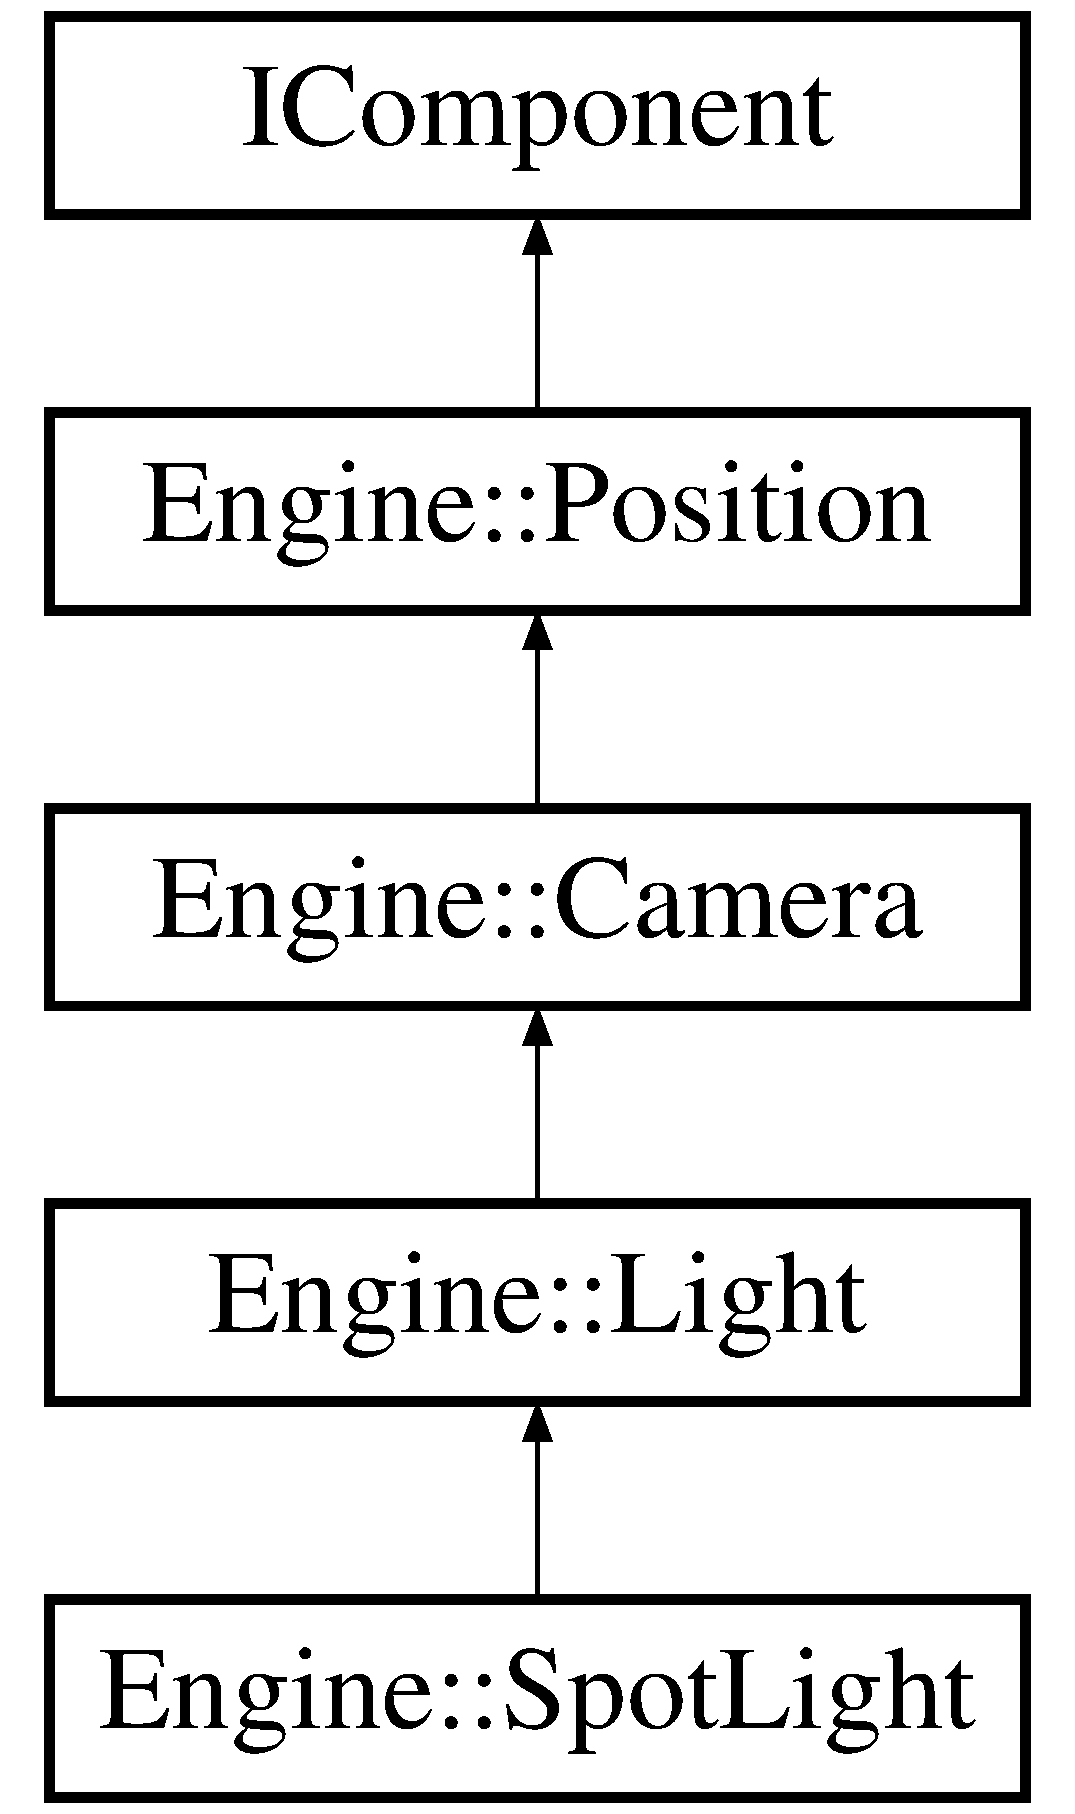
\includegraphics[height=5.000000cm]{classEngine_1_1Camera}
\end{center}
\end{figure}
\subsection*{Public Types}
\begin{DoxyCompactItemize}
\item 
enum \hyperlink{classEngine_1_1Camera_a54aed52433cefef871f5d0b294b7e87b}{Direction} \{ {\bfseries F\+O\+R\+W\+A\+R\+D}, 
{\bfseries B\+A\+C\+K\+W\+A\+R\+D}, 
{\bfseries L\+E\+F\+T}, 
{\bfseries R\+I\+G\+H\+T}
 \}\begin{DoxyCompactList}\small\item\em The Direction enum. \end{DoxyCompactList}
\item 
\hypertarget{classEngine_1_1Camera_a4362ae70fbe23d07e449fdfef964c36c}{}enum {\bfseries Camera\+Mode} \{ {\bfseries F\+L\+Y\+\_\+\+M\+O\+D\+E}, 
{\bfseries E\+G\+O\+\_\+\+M\+O\+D\+E}
 \}\label{classEngine_1_1Camera_a4362ae70fbe23d07e449fdfef964c36c}

\end{DoxyCompactItemize}
\subsection*{Public Member Functions}
\begin{DoxyCompactItemize}
\item 
\hyperlink{classEngine_1_1Camera_a5c68f1ee8348320a6c47419ae2d724fb}{Camera} (void)
\begin{DoxyCompactList}\small\item\em \hyperlink{classEngine_1_1Camera}{Camera}. \end{DoxyCompactList}\item 
\hyperlink{classEngine_1_1Camera_afdc243ad39091e737778367b9925091d}{Camera} (const std\+::string \&camera\+\_\+name)
\begin{DoxyCompactList}\small\item\em \hyperlink{classEngine_1_1Camera}{Camera}. \end{DoxyCompactList}\item 
void \hyperlink{classEngine_1_1Camera_a1d5813e53c9c0eac322b079c211eb7a8}{set\+Scissor\+View} (\hyperlink{classVector4}{Vector4f} sci)
\begin{DoxyCompactList}\small\item\em set\+View \end{DoxyCompactList}\item 
\hypertarget{classEngine_1_1Camera_a863693ca42f6a9e5f0d1983af4c55b04}{}void {\bfseries set\+Scissor\+View} (int x, int y, int width, int height)\label{classEngine_1_1Camera_a863693ca42f6a9e5f0d1983af4c55b04}

\item 
void \hyperlink{classEngine_1_1Camera_a6af03781efc6da99e021a5165634627f}{set\+Name} (const std\+::string \&name)
\begin{DoxyCompactList}\small\item\em set\+Name \end{DoxyCompactList}\item 
void \hyperlink{classEngine_1_1Camera_a2de0f59bf133c8c242423a5812399166}{set\+Mode} (Camera\+Mode mode)
\begin{DoxyCompactList}\small\item\em set\+Mode \end{DoxyCompactList}\item 
\hypertarget{classEngine_1_1Camera_a83c9aa8c07f1b67b179e0708cfe427a6}{}void {\bfseries invert\+Pitch} (void)\label{classEngine_1_1Camera_a83c9aa8c07f1b67b179e0708cfe427a6}

\item 
\hypertarget{classEngine_1_1Camera_ab9ad7d4d0158ab8f3580f50244d5e67e}{}void {\bfseries invert\+Yaw} (void)\label{classEngine_1_1Camera_ab9ad7d4d0158ab8f3580f50244d5e67e}

\item 
\hyperlink{classVector4}{Vector4f} \hyperlink{classEngine_1_1Camera_a433f03de6ad715da69536f8e521dd8c7}{get\+View} (void)
\begin{DoxyCompactList}\small\item\em get\+View \end{DoxyCompactList}\item 
std\+::string \hyperlink{classEngine_1_1Camera_a1ac6dd58e8986f523dabcf4e91e04a26}{get\+Name} (void)
\begin{DoxyCompactList}\small\item\em get\+Name \end{DoxyCompactList}\item 
void \hyperlink{classEngine_1_1Camera_a13c461546b6141eb6baabb54419e6476}{Auto\+Rotation} (\hyperlink{classEngine_1_1Position}{Position} $\ast$object)
\begin{DoxyCompactList}\small\item\em follow \end{DoxyCompactList}\item 
\hypertarget{classEngine_1_1Camera_a000392f7de2ae12bed38baed2449872d}{}void {\bfseries Auto\+Rotation\+Reset} (void)\label{classEngine_1_1Camera_a000392f7de2ae12bed38baed2449872d}

\item 
void \hyperlink{classEngine_1_1Camera_a3261c7dbede2662496927861f19dbd92}{move} (\hyperlink{classEngine_1_1Camera_a54aed52433cefef871f5d0b294b7e87b}{Direction} dir, float speed)
\begin{DoxyCompactList}\small\item\em move \end{DoxyCompactList}\item 
\hypertarget{classEngine_1_1Camera_a9ab2ad1245b516e2a51f6007c2b2d9c3}{}void {\bfseries move\+\_\+ex} (\hyperlink{classEngine_1_1Camera_a54aed52433cefef871f5d0b294b7e87b}{Camera\+::\+Direction} dir, float distance, \hyperlink{classEngine_1_1Position}{Position} $\ast$object)\label{classEngine_1_1Camera_a9ab2ad1245b516e2a51f6007c2b2d9c3}

\item 
float \hyperlink{classEngine_1_1Camera_ab71919b625658e16ea5664609d4fe30f}{get\+Pitch} (void)
\begin{DoxyCompactList}\small\item\em get\+Pitch \end{DoxyCompactList}\item 
float \hyperlink{classEngine_1_1Camera_a9c53dd61301fd51e532d5ba77c5e14dd}{get\+Yaw} (void)
\begin{DoxyCompactList}\small\item\em get\+Yaw \end{DoxyCompactList}\item 
void \hyperlink{classEngine_1_1Camera_ae37c21a512277b455ac79f57cc573be4}{transform} (void)
\begin{DoxyCompactList}\small\item\em transform \end{DoxyCompactList}\item 
void \hyperlink{classEngine_1_1Camera_a6d2bbb5124335a8cb3e7e871b4f5216b}{set\+Pitch} (float value)
\begin{DoxyCompactList}\small\item\em set\+Pitch \end{DoxyCompactList}\item 
void \hyperlink{classEngine_1_1Camera_aecaf00e8167268dec5f1745d3db06fd0}{set\+Yaw} (float value)
\begin{DoxyCompactList}\small\item\em set\+Yaw \end{DoxyCompactList}\end{DoxyCompactItemize}
\subsection*{Protected Member Functions}
\begin{DoxyCompactItemize}
\item 
float \hyperlink{classEngine_1_1Camera_a2d6b55fc92f272ab3e53833e8d069d7a}{get\+Radian} (float angle)
\begin{DoxyCompactList}\small\item\em get\+Radian \end{DoxyCompactList}\end{DoxyCompactItemize}


\subsection{Detailed Description}
The \hyperlink{classEngine_1_1Camera}{Camera} class. 

\subsection{Member Enumeration Documentation}
\hypertarget{classEngine_1_1Camera_a54aed52433cefef871f5d0b294b7e87b}{}\index{Engine\+::\+Camera@{Engine\+::\+Camera}!Direction@{Direction}}
\index{Direction@{Direction}!Engine\+::\+Camera@{Engine\+::\+Camera}}
\subsubsection[{Direction}]{\setlength{\rightskip}{0pt plus 5cm}enum {\bf Engine\+::\+Camera\+::\+Direction}}\label{classEngine_1_1Camera_a54aed52433cefef871f5d0b294b7e87b}


The Direction enum. 

Movement directions 

\subsection{Constructor \& Destructor Documentation}
\hypertarget{classEngine_1_1Camera_a5c68f1ee8348320a6c47419ae2d724fb}{}\index{Engine\+::\+Camera@{Engine\+::\+Camera}!Camera@{Camera}}
\index{Camera@{Camera}!Engine\+::\+Camera@{Engine\+::\+Camera}}
\subsubsection[{Camera(void)}]{\setlength{\rightskip}{0pt plus 5cm}Camera\+::\+Camera (
\begin{DoxyParamCaption}
\item[{void}]{}
\end{DoxyParamCaption}
)\hspace{0.3cm}{\ttfamily [explicit]}}\label{classEngine_1_1Camera_a5c68f1ee8348320a6c47419ae2d724fb}


\hyperlink{classEngine_1_1Camera}{Camera}. 

Create Default \hyperlink{classEngine_1_1Camera}{Camera} ( aka Main ) \hypertarget{classEngine_1_1Camera_afdc243ad39091e737778367b9925091d}{}\index{Engine\+::\+Camera@{Engine\+::\+Camera}!Camera@{Camera}}
\index{Camera@{Camera}!Engine\+::\+Camera@{Engine\+::\+Camera}}
\subsubsection[{Camera(const std\+::string \&camera\+\_\+name)}]{\setlength{\rightskip}{0pt plus 5cm}Engine\+::\+Camera\+::\+Camera (
\begin{DoxyParamCaption}
\item[{const std\+::string \&}]{camera\+\_\+name}
\end{DoxyParamCaption}
)\hspace{0.3cm}{\ttfamily [explicit]}}\label{classEngine_1_1Camera_afdc243ad39091e737778367b9925091d}


\hyperlink{classEngine_1_1Camera}{Camera}. 

Create S\+C\+I\+S\+S\+O\+R \hyperlink{classEngine_1_1Camera}{Camera} 
\begin{DoxyParams}{Parameters}
{\em camera\+\_\+name} & \\
\hline
\end{DoxyParams}


\subsection{Member Function Documentation}
\hypertarget{classEngine_1_1Camera_a13c461546b6141eb6baabb54419e6476}{}\index{Engine\+::\+Camera@{Engine\+::\+Camera}!Auto\+Rotation@{Auto\+Rotation}}
\index{Auto\+Rotation@{Auto\+Rotation}!Engine\+::\+Camera@{Engine\+::\+Camera}}
\subsubsection[{Auto\+Rotation(\+Position $\ast$object)}]{\setlength{\rightskip}{0pt plus 5cm}void Camera\+::\+Auto\+Rotation (
\begin{DoxyParamCaption}
\item[{{\bf Position} $\ast$}]{object}
\end{DoxyParamCaption}
)}\label{classEngine_1_1Camera_a13c461546b6141eb6baabb54419e6476}


follow 

\hyperlink{classEngine_1_1Camera}{Camera} follow a Object 
\begin{DoxyParams}{Parameters}
{\em object} & \\
\hline
\end{DoxyParams}
\hypertarget{classEngine_1_1Camera_a1ac6dd58e8986f523dabcf4e91e04a26}{}\index{Engine\+::\+Camera@{Engine\+::\+Camera}!get\+Name@{get\+Name}}
\index{get\+Name@{get\+Name}!Engine\+::\+Camera@{Engine\+::\+Camera}}
\subsubsection[{get\+Name(void)}]{\setlength{\rightskip}{0pt plus 5cm}std\+::string Camera\+::get\+Name (
\begin{DoxyParamCaption}
\item[{void}]{}
\end{DoxyParamCaption}
)}\label{classEngine_1_1Camera_a1ac6dd58e8986f523dabcf4e91e04a26}


get\+Name 

Return \hyperlink{classEngine_1_1Camera}{Camera} Name \begin{DoxyReturn}{Returns}

\end{DoxyReturn}
\hypertarget{classEngine_1_1Camera_ab71919b625658e16ea5664609d4fe30f}{}\index{Engine\+::\+Camera@{Engine\+::\+Camera}!get\+Pitch@{get\+Pitch}}
\index{get\+Pitch@{get\+Pitch}!Engine\+::\+Camera@{Engine\+::\+Camera}}
\subsubsection[{get\+Pitch(void)}]{\setlength{\rightskip}{0pt plus 5cm}float Camera\+::get\+Pitch (
\begin{DoxyParamCaption}
\item[{void}]{}
\end{DoxyParamCaption}
)}\label{classEngine_1_1Camera_ab71919b625658e16ea5664609d4fe30f}


get\+Pitch 

Return Pitch value \begin{DoxyReturn}{Returns}

\end{DoxyReturn}
\hypertarget{classEngine_1_1Camera_a2d6b55fc92f272ab3e53833e8d069d7a}{}\index{Engine\+::\+Camera@{Engine\+::\+Camera}!get\+Radian@{get\+Radian}}
\index{get\+Radian@{get\+Radian}!Engine\+::\+Camera@{Engine\+::\+Camera}}
\subsubsection[{get\+Radian(float angle)}]{\setlength{\rightskip}{0pt plus 5cm}float Camera\+::get\+Radian (
\begin{DoxyParamCaption}
\item[{float}]{angle}
\end{DoxyParamCaption}
)\hspace{0.3cm}{\ttfamily [inline]}, {\ttfamily [protected]}}\label{classEngine_1_1Camera_a2d6b55fc92f272ab3e53833e8d069d7a}


get\+Radian 

Calc Angle to Radian 
\begin{DoxyParams}{Parameters}
{\em angle} & \\
\hline
\end{DoxyParams}
\begin{DoxyReturn}{Returns}

\end{DoxyReturn}
\hypertarget{classEngine_1_1Camera_a433f03de6ad715da69536f8e521dd8c7}{}\index{Engine\+::\+Camera@{Engine\+::\+Camera}!get\+View@{get\+View}}
\index{get\+View@{get\+View}!Engine\+::\+Camera@{Engine\+::\+Camera}}
\subsubsection[{get\+View(void)}]{\setlength{\rightskip}{0pt plus 5cm}{\bf Vector4f} Camera\+::get\+View (
\begin{DoxyParamCaption}
\item[{void}]{}
\end{DoxyParamCaption}
)}\label{classEngine_1_1Camera_a433f03de6ad715da69536f8e521dd8c7}


get\+View 

Return Scissor Values \begin{DoxyReturn}{Returns}

\end{DoxyReturn}
\hypertarget{classEngine_1_1Camera_a9c53dd61301fd51e532d5ba77c5e14dd}{}\index{Engine\+::\+Camera@{Engine\+::\+Camera}!get\+Yaw@{get\+Yaw}}
\index{get\+Yaw@{get\+Yaw}!Engine\+::\+Camera@{Engine\+::\+Camera}}
\subsubsection[{get\+Yaw(void)}]{\setlength{\rightskip}{0pt plus 5cm}float Camera\+::get\+Yaw (
\begin{DoxyParamCaption}
\item[{void}]{}
\end{DoxyParamCaption}
)}\label{classEngine_1_1Camera_a9c53dd61301fd51e532d5ba77c5e14dd}


get\+Yaw 

Return Yaw Value \begin{DoxyReturn}{Returns}

\end{DoxyReturn}
\hypertarget{classEngine_1_1Camera_a3261c7dbede2662496927861f19dbd92}{}\index{Engine\+::\+Camera@{Engine\+::\+Camera}!move@{move}}
\index{move@{move}!Engine\+::\+Camera@{Engine\+::\+Camera}}
\subsubsection[{move(\+Direction dir, float speed)}]{\setlength{\rightskip}{0pt plus 5cm}void Camera\+::move (
\begin{DoxyParamCaption}
\item[{{\bf Camera\+::\+Direction}}]{dir, }
\item[{float}]{speed}
\end{DoxyParamCaption}
)}\label{classEngine_1_1Camera_a3261c7dbede2662496927861f19dbd92}


move 

Move \hyperlink{classEngine_1_1Camera}{Camera} to direction with speed 
\begin{DoxyParams}{Parameters}
{\em dir} & \+: Direction ( F\+O\+R\+W\+A\+R\+D...) \\
\hline
{\em speed} & \+: Speed \\
\hline
\end{DoxyParams}
\hypertarget{classEngine_1_1Camera_a2de0f59bf133c8c242423a5812399166}{}\index{Engine\+::\+Camera@{Engine\+::\+Camera}!set\+Mode@{set\+Mode}}
\index{set\+Mode@{set\+Mode}!Engine\+::\+Camera@{Engine\+::\+Camera}}
\subsubsection[{set\+Mode(\+Camera\+Mode mode)}]{\setlength{\rightskip}{0pt plus 5cm}void Camera\+::set\+Mode (
\begin{DoxyParamCaption}
\item[{Camera\+Mode}]{mode}
\end{DoxyParamCaption}
)}\label{classEngine_1_1Camera_a2de0f59bf133c8c242423a5812399166}


set\+Mode 


\begin{DoxyParams}{Parameters}
{\em mode} & \\
\hline
\end{DoxyParams}
\hypertarget{classEngine_1_1Camera_a6af03781efc6da99e021a5165634627f}{}\index{Engine\+::\+Camera@{Engine\+::\+Camera}!set\+Name@{set\+Name}}
\index{set\+Name@{set\+Name}!Engine\+::\+Camera@{Engine\+::\+Camera}}
\subsubsection[{set\+Name(const std\+::string \&name)}]{\setlength{\rightskip}{0pt plus 5cm}void Camera\+::set\+Name (
\begin{DoxyParamCaption}
\item[{const std\+::string \&}]{name}
\end{DoxyParamCaption}
)}\label{classEngine_1_1Camera_a6af03781efc6da99e021a5165634627f}


set\+Name 

Set \hyperlink{classEngine_1_1Camera}{Camera} Name 
\begin{DoxyParams}{Parameters}
{\em name} & \\
\hline
\end{DoxyParams}
\hypertarget{classEngine_1_1Camera_a6d2bbb5124335a8cb3e7e871b4f5216b}{}\index{Engine\+::\+Camera@{Engine\+::\+Camera}!set\+Pitch@{set\+Pitch}}
\index{set\+Pitch@{set\+Pitch}!Engine\+::\+Camera@{Engine\+::\+Camera}}
\subsubsection[{set\+Pitch(float value)}]{\setlength{\rightskip}{0pt plus 5cm}void Camera\+::set\+Pitch (
\begin{DoxyParamCaption}
\item[{float}]{value}
\end{DoxyParamCaption}
)}\label{classEngine_1_1Camera_a6d2bbb5124335a8cb3e7e871b4f5216b}


set\+Pitch 

Set Pitch value \hypertarget{classEngine_1_1Camera_a1d5813e53c9c0eac322b079c211eb7a8}{}\index{Engine\+::\+Camera@{Engine\+::\+Camera}!set\+Scissor\+View@{set\+Scissor\+View}}
\index{set\+Scissor\+View@{set\+Scissor\+View}!Engine\+::\+Camera@{Engine\+::\+Camera}}
\subsubsection[{set\+Scissor\+View(\+Vector4f sci)}]{\setlength{\rightskip}{0pt plus 5cm}void Camera\+::set\+Scissor\+View (
\begin{DoxyParamCaption}
\item[{{\bf Vector4f}}]{sci}
\end{DoxyParamCaption}
)}\label{classEngine_1_1Camera_a1d5813e53c9c0eac322b079c211eb7a8}


set\+View 

Set View\+Port Values for S\+C\+I\+S\+S\+O\+R \hyperlink{classEngine_1_1Camera}{Camera} 
\begin{DoxyParams}{Parameters}
{\em x} & \\
\hline
{\em y} & \\
\hline
{\em with} & \\
\hline
{\em height} & \\
\hline
\end{DoxyParams}
\hypertarget{classEngine_1_1Camera_aecaf00e8167268dec5f1745d3db06fd0}{}\index{Engine\+::\+Camera@{Engine\+::\+Camera}!set\+Yaw@{set\+Yaw}}
\index{set\+Yaw@{set\+Yaw}!Engine\+::\+Camera@{Engine\+::\+Camera}}
\subsubsection[{set\+Yaw(float value)}]{\setlength{\rightskip}{0pt plus 5cm}void Camera\+::set\+Yaw (
\begin{DoxyParamCaption}
\item[{float}]{value}
\end{DoxyParamCaption}
)}\label{classEngine_1_1Camera_aecaf00e8167268dec5f1745d3db06fd0}


set\+Yaw 

Set Yaw value 
\begin{DoxyParams}{Parameters}
{\em value} & \\
\hline
\end{DoxyParams}
\hypertarget{classEngine_1_1Camera_ae37c21a512277b455ac79f57cc573be4}{}\index{Engine\+::\+Camera@{Engine\+::\+Camera}!transform@{transform}}
\index{transform@{transform}!Engine\+::\+Camera@{Engine\+::\+Camera}}
\subsubsection[{transform(void)}]{\setlength{\rightskip}{0pt plus 5cm}void Camera\+::transform (
\begin{DoxyParamCaption}
\item[{void}]{}
\end{DoxyParamCaption}
)}\label{classEngine_1_1Camera_ae37c21a512277b455ac79f57cc573be4}


transform 

\hyperlink{classEngine_1_1Camera}{Camera} transformation 

The documentation for this class was generated from the following files\+:\begin{DoxyCompactItemize}
\item 
include/\+Container/camera.\+h\item 
Container/Camera.\+cpp\end{DoxyCompactItemize}

\hypertarget{classEngine_1_1CameraManager}{}\section{Engine\+:\+:Camera\+Manager Class Reference}
\label{classEngine_1_1CameraManager}\index{Engine\+::\+Camera\+Manager@{Engine\+::\+Camera\+Manager}}


The \hyperlink{classEngine_1_1CameraManager}{Camera\+Manager} controlled Cameras.  




{\ttfamily \#include $<$cameramanager.\+h$>$}

\subsection*{Public Types}
\begin{DoxyCompactItemize}
\item 
using \hyperlink{classEngine_1_1CameraManager_aadc529c6b245d7b6f57774bba20f1c21}{Cameras} = std\+::list$<$ \hyperlink{classEngine_1_1Camera}{Camera} $\ast$ $>$
\item 
using \hyperlink{classEngine_1_1CameraManager_a9ec0ae8ac0232b41f018af98f57c1f6b}{Camera\+Map} = std\+::map$<$ uint, \hyperlink{classEngine_1_1Camera}{Camera} $\ast$ $>$
\end{DoxyCompactItemize}
\subsection*{Public Member Functions}
\begin{DoxyCompactItemize}
\item 
\hypertarget{classEngine_1_1CameraManager_ada4e1659dc34f63e8feb300a5425ab33}{}void {\bfseries finish} (void)\label{classEngine_1_1CameraManager_ada4e1659dc34f63e8feb300a5425ab33}

\item 
\hyperlink{classEngine_1_1Camera}{Camera} $\ast$ \hyperlink{classEngine_1_1CameraManager_a1ba4fff2c27f8e71b42db9df1411c87b}{create\+Camera} (void)
\begin{DoxyCompactList}\small\item\em create\+Camera \end{DoxyCompactList}\item 
\hyperlink{classEngine_1_1Camera}{Camera} $\ast$ \hyperlink{classEngine_1_1CameraManager_ab5ca3c3c1d5e47197c77359c406caf80}{create\+Camera} (const std\+::string \&camera\+\_\+name, const \hyperlink{classVector4}{Vector4f} \&scissor\+\_\+values)
\begin{DoxyCompactList}\small\item\em Render\+Manager\+::create\+Camera. \end{DoxyCompactList}\item 
\hyperlink{classEngine_1_1Camera}{Camera} $\ast$ \hyperlink{classEngine_1_1CameraManager_a1944ff084f6aa681f1d04baf26880fde}{get\+Camera} (const std\+::string \&camera\+\_\+name)
\begin{DoxyCompactList}\small\item\em get\+Camera \end{DoxyCompactList}\item 
\hyperlink{classEngine_1_1Camera}{Camera} $\ast$ \hyperlink{classEngine_1_1CameraManager_acc64e137d415f4a79b704a4abc506c1e}{get\+Camera} (uint component\+\_\+id)
\begin{DoxyCompactList}\small\item\em get\+Camera \end{DoxyCompactList}\item 
\hyperlink{classEngine_1_1CameraManager_aadc529c6b245d7b6f57774bba20f1c21}{Cameras} \hyperlink{classEngine_1_1CameraManager_ad0d91631c2ac9451a7d92e353f266740}{get\+Cameras} (void)
\begin{DoxyCompactList}\small\item\em get\+Cameras \end{DoxyCompactList}\item 
void \hyperlink{classEngine_1_1CameraManager_a684eae9f1a8ad86d55be797c7531739a}{add\+Camera} (\hyperlink{classEngine_1_1Camera}{Camera} $\ast$camera)
\begin{DoxyCompactList}\small\item\em add\+Camera \end{DoxyCompactList}\item 
void \hyperlink{classEngine_1_1CameraManager_a7b3d0de66044139377679bc5791a887e}{Bind\+Camera} (uint component\+\_\+id, \hyperlink{classEngine_1_1Camera}{Camera} $\ast$camera)
\begin{DoxyCompactList}\small\item\em Bind\+Camera. \end{DoxyCompactList}\item 
void \hyperlink{classEngine_1_1CameraManager_a6d55a74104cd4a15a4522bef410ee53e}{remove} (\hyperlink{classEngine_1_1Camera}{Camera} $\ast$camera)
\begin{DoxyCompactList}\small\item\em remove \end{DoxyCompactList}\end{DoxyCompactItemize}
\subsection*{Static Public Member Functions}
\begin{DoxyCompactItemize}
\item 
static \hyperlink{classEngine_1_1CameraManager}{Camera\+Manager} $\ast$ \hyperlink{classEngine_1_1CameraManager_af980601c66f5441cfdd7cf3affe156f5}{get\+Singleton\+Ptr} (void)
\begin{DoxyCompactList}\small\item\em get\+Singleton\+Ptr \end{DoxyCompactList}\end{DoxyCompactItemize}


\subsection{Detailed Description}
The \hyperlink{classEngine_1_1CameraManager}{Camera\+Manager} controlled Cameras. 

Management of Cameras


\begin{DoxyItemize}
\item create Cameras
\item delete Cameras
\item Main \hyperlink{classEngine_1_1Camera}{Camera} \& Scissor Cameras 
\end{DoxyItemize}

\subsection{Member Typedef Documentation}
\hypertarget{classEngine_1_1CameraManager_a9ec0ae8ac0232b41f018af98f57c1f6b}{}\index{Engine\+::\+Camera\+Manager@{Engine\+::\+Camera\+Manager}!Camera\+Map@{Camera\+Map}}
\index{Camera\+Map@{Camera\+Map}!Engine\+::\+Camera\+Manager@{Engine\+::\+Camera\+Manager}}
\subsubsection[{Camera\+Map}]{\setlength{\rightskip}{0pt plus 5cm}using {\bf Engine\+::\+Camera\+Manager\+::\+Camera\+Map} =  std\+::map$<$ uint , {\bf Camera} $\ast$ $>$}\label{classEngine_1_1CameraManager_a9ec0ae8ac0232b41f018af98f57c1f6b}
Map of Cameras with Component I\+Ds \hypertarget{classEngine_1_1CameraManager_aadc529c6b245d7b6f57774bba20f1c21}{}\index{Engine\+::\+Camera\+Manager@{Engine\+::\+Camera\+Manager}!Cameras@{Cameras}}
\index{Cameras@{Cameras}!Engine\+::\+Camera\+Manager@{Engine\+::\+Camera\+Manager}}
\subsubsection[{Cameras}]{\setlength{\rightskip}{0pt plus 5cm}using {\bf Engine\+::\+Camera\+Manager\+::\+Cameras} =  std\+::list$<$ {\bf Camera} $\ast$ $>$}\label{classEngine_1_1CameraManager_aadc529c6b245d7b6f57774bba20f1c21}
List of Cameras 

\subsection{Member Function Documentation}
\hypertarget{classEngine_1_1CameraManager_a684eae9f1a8ad86d55be797c7531739a}{}\index{Engine\+::\+Camera\+Manager@{Engine\+::\+Camera\+Manager}!add\+Camera@{add\+Camera}}
\index{add\+Camera@{add\+Camera}!Engine\+::\+Camera\+Manager@{Engine\+::\+Camera\+Manager}}
\subsubsection[{add\+Camera(\+Camera $\ast$camera)}]{\setlength{\rightskip}{0pt plus 5cm}void Camera\+Manager\+::add\+Camera (
\begin{DoxyParamCaption}
\item[{{\bf Camera} $\ast$}]{camera}
\end{DoxyParamCaption}
)}\label{classEngine_1_1CameraManager_a684eae9f1a8ad86d55be797c7531739a}


add\+Camera 

Save \hyperlink{classEngine_1_1Camera}{Camera} 
\begin{DoxyParams}{Parameters}
{\em camera} & \\
\hline
\end{DoxyParams}
\hypertarget{classEngine_1_1CameraManager_a7b3d0de66044139377679bc5791a887e}{}\index{Engine\+::\+Camera\+Manager@{Engine\+::\+Camera\+Manager}!Bind\+Camera@{Bind\+Camera}}
\index{Bind\+Camera@{Bind\+Camera}!Engine\+::\+Camera\+Manager@{Engine\+::\+Camera\+Manager}}
\subsubsection[{Bind\+Camera(uint component\+\_\+id, Camera $\ast$camera)}]{\setlength{\rightskip}{0pt plus 5cm}void Camera\+Manager\+::\+Bind\+Camera (
\begin{DoxyParamCaption}
\item[{uint}]{component\+\_\+id, }
\item[{{\bf Camera} $\ast$}]{camera}
\end{DoxyParamCaption}
)}\label{classEngine_1_1CameraManager_a7b3d0de66044139377679bc5791a887e}


Bind\+Camera. 

Bind a \hyperlink{classEngine_1_1Camera}{Camera} with a Component 
\begin{DoxyParams}{Parameters}
{\em component\+\_\+id} & \\
\hline
{\em camera} & \\
\hline
\end{DoxyParams}
\hypertarget{classEngine_1_1CameraManager_a1ba4fff2c27f8e71b42db9df1411c87b}{}\index{Engine\+::\+Camera\+Manager@{Engine\+::\+Camera\+Manager}!create\+Camera@{create\+Camera}}
\index{create\+Camera@{create\+Camera}!Engine\+::\+Camera\+Manager@{Engine\+::\+Camera\+Manager}}
\subsubsection[{create\+Camera(void)}]{\setlength{\rightskip}{0pt plus 5cm}{\bf Camera} $\ast$ Camera\+Manager\+::create\+Camera (
\begin{DoxyParamCaption}
\item[{void}]{}
\end{DoxyParamCaption}
)}\label{classEngine_1_1CameraManager_a1ba4fff2c27f8e71b42db9df1411c87b}


create\+Camera 

Create a Main \hyperlink{classEngine_1_1Camera}{Camera} 
\begin{DoxyParams}{Parameters}
{\em camera\+\_\+name} & \\
\hline
\end{DoxyParams}
\begin{DoxyReturn}{Returns}

\end{DoxyReturn}
\hypertarget{classEngine_1_1CameraManager_ab5ca3c3c1d5e47197c77359c406caf80}{}\index{Engine\+::\+Camera\+Manager@{Engine\+::\+Camera\+Manager}!create\+Camera@{create\+Camera}}
\index{create\+Camera@{create\+Camera}!Engine\+::\+Camera\+Manager@{Engine\+::\+Camera\+Manager}}
\subsubsection[{create\+Camera(const std\+::string \&camera\+\_\+name, const Vector4f \&scissor\+\_\+values)}]{\setlength{\rightskip}{0pt plus 5cm}{\bf Camera} $\ast$ Camera\+Manager\+::create\+Camera (
\begin{DoxyParamCaption}
\item[{const std\+::string \&}]{camera\+\_\+name, }
\item[{const {\bf Vector4f} \&}]{scissor\+\_\+values}
\end{DoxyParamCaption}
)}\label{classEngine_1_1CameraManager_ab5ca3c3c1d5e47197c77359c406caf80}


Render\+Manager\+::create\+Camera. 

Create Scissor \hyperlink{classEngine_1_1Camera}{Camera} --- for Minimaps or otherwise


\begin{DoxyParams}{Parameters}
{\em camera\+\_\+name} & \\
\hline
{\em scissor\+\_\+values} & ( x , y , width , height ) \\
\hline
\end{DoxyParams}
\begin{DoxyReturn}{Returns}

\end{DoxyReturn}
\hypertarget{classEngine_1_1CameraManager_a1944ff084f6aa681f1d04baf26880fde}{}\index{Engine\+::\+Camera\+Manager@{Engine\+::\+Camera\+Manager}!get\+Camera@{get\+Camera}}
\index{get\+Camera@{get\+Camera}!Engine\+::\+Camera\+Manager@{Engine\+::\+Camera\+Manager}}
\subsubsection[{get\+Camera(const std\+::string \&camera\+\_\+name)}]{\setlength{\rightskip}{0pt plus 5cm}{\bf Camera} $\ast$ Camera\+Manager\+::get\+Camera (
\begin{DoxyParamCaption}
\item[{const std\+::string \&}]{camera\+\_\+name}
\end{DoxyParamCaption}
)}\label{classEngine_1_1CameraManager_a1944ff084f6aa681f1d04baf26880fde}


get\+Camera 

Return \hyperlink{classEngine_1_1Camera}{Camera} by Name 
\begin{DoxyParams}{Parameters}
{\em camera\+\_\+name} & \\
\hline
\end{DoxyParams}
\begin{DoxyReturn}{Returns}

\end{DoxyReturn}
\hypertarget{classEngine_1_1CameraManager_acc64e137d415f4a79b704a4abc506c1e}{}\index{Engine\+::\+Camera\+Manager@{Engine\+::\+Camera\+Manager}!get\+Camera@{get\+Camera}}
\index{get\+Camera@{get\+Camera}!Engine\+::\+Camera\+Manager@{Engine\+::\+Camera\+Manager}}
\subsubsection[{get\+Camera(uint component\+\_\+id)}]{\setlength{\rightskip}{0pt plus 5cm}{\bf Camera} $\ast$ Camera\+Manager\+::get\+Camera (
\begin{DoxyParamCaption}
\item[{uint}]{component\+\_\+id}
\end{DoxyParamCaption}
)}\label{classEngine_1_1CameraManager_acc64e137d415f4a79b704a4abc506c1e}


get\+Camera 

Return \hyperlink{classEngine_1_1Camera}{Camera} by Component Id 
\begin{DoxyParams}{Parameters}
{\em component\+\_\+id} & \\
\hline
\end{DoxyParams}
\begin{DoxyReturn}{Returns}

\end{DoxyReturn}
\hypertarget{classEngine_1_1CameraManager_ad0d91631c2ac9451a7d92e353f266740}{}\index{Engine\+::\+Camera\+Manager@{Engine\+::\+Camera\+Manager}!get\+Cameras@{get\+Cameras}}
\index{get\+Cameras@{get\+Cameras}!Engine\+::\+Camera\+Manager@{Engine\+::\+Camera\+Manager}}
\subsubsection[{get\+Cameras(void)}]{\setlength{\rightskip}{0pt plus 5cm}{\bf Cameras} Engine\+::\+Camera\+Manager\+::get\+Cameras (
\begin{DoxyParamCaption}
\item[{void}]{}
\end{DoxyParamCaption}
)}\label{classEngine_1_1CameraManager_ad0d91631c2ac9451a7d92e353f266740}


get\+Cameras 

Return Cameras \begin{DoxyReturn}{Returns}

\end{DoxyReturn}
\hypertarget{classEngine_1_1CameraManager_af980601c66f5441cfdd7cf3affe156f5}{}\index{Engine\+::\+Camera\+Manager@{Engine\+::\+Camera\+Manager}!get\+Singleton\+Ptr@{get\+Singleton\+Ptr}}
\index{get\+Singleton\+Ptr@{get\+Singleton\+Ptr}!Engine\+::\+Camera\+Manager@{Engine\+::\+Camera\+Manager}}
\subsubsection[{get\+Singleton\+Ptr(void)}]{\setlength{\rightskip}{0pt plus 5cm}{\bf Camera\+Manager} $\ast$ Camera\+Manager\+::get\+Singleton\+Ptr (
\begin{DoxyParamCaption}
\item[{void}]{}
\end{DoxyParamCaption}
)\hspace{0.3cm}{\ttfamily [static]}}\label{classEngine_1_1CameraManager_af980601c66f5441cfdd7cf3affe156f5}


get\+Singleton\+Ptr 

Return \hyperlink{classEngine_1_1Camera}{Camera} Manager Instance \begin{DoxyReturn}{Returns}

\end{DoxyReturn}
\hypertarget{classEngine_1_1CameraManager_a6d55a74104cd4a15a4522bef410ee53e}{}\index{Engine\+::\+Camera\+Manager@{Engine\+::\+Camera\+Manager}!remove@{remove}}
\index{remove@{remove}!Engine\+::\+Camera\+Manager@{Engine\+::\+Camera\+Manager}}
\subsubsection[{remove(\+Camera $\ast$camera)}]{\setlength{\rightskip}{0pt plus 5cm}void Camera\+Manager\+::remove (
\begin{DoxyParamCaption}
\item[{{\bf Camera} $\ast$}]{camera}
\end{DoxyParamCaption}
)}\label{classEngine_1_1CameraManager_a6d55a74104cd4a15a4522bef410ee53e}


remove 

Remove \hyperlink{classEngine_1_1Camera}{Camera} from list and destroy it 
\begin{DoxyParams}{Parameters}
{\em camera} & \\
\hline
\end{DoxyParams}


The documentation for this class was generated from the following files\+:\begin{DoxyCompactItemize}
\item 
include/\+Manager/cameramanager.\+h\item 
Engine/\+Manager/Camera\+Manager.\+cpp\end{DoxyCompactItemize}

\hypertarget{classEngine_1_1Config}{}\section{Engine\+:\+:Config Class Reference}
\label{classEngine_1_1Config}\index{Engine\+::\+Config@{Engine\+::\+Config}}
\subsection*{Public Member Functions}
\begin{DoxyCompactItemize}
\item 
\hypertarget{classEngine_1_1Config_aedb3f3bcd87a7d860bb00f3480ce61d3}{}{\bfseries Config} (const std\+::string \&file\+\_\+name)\label{classEngine_1_1Config_aedb3f3bcd87a7d860bb00f3480ce61d3}

\item 
\hypertarget{classEngine_1_1Config_a86838f5990d86836d1d33d68c33f1b83}{}virtual void {\bfseries load} (void)\label{classEngine_1_1Config_a86838f5990d86836d1d33d68c33f1b83}

\item 
\hypertarget{classEngine_1_1Config_a55c0b956008149bc059afa6f9ff78a67}{}void {\bfseries add\+Function} (const std\+::string \&value, C\+O\+N\+F\+I\+G\+\_\+\+F\+U\+N\+C func)\label{classEngine_1_1Config_a55c0b956008149bc059afa6f9ff78a67}

\end{DoxyCompactItemize}
\subsection*{Protected Attributes}
\begin{DoxyCompactItemize}
\item 
\hypertarget{classEngine_1_1Config_a4a6bd1120b3e16a684c1647ebc51cab3}{}std\+::string {\bfseries m\+File\+Name}\label{classEngine_1_1Config_a4a6bd1120b3e16a684c1647ebc51cab3}

\item 
\hypertarget{classEngine_1_1Config_a98196653c44474724605aa4e321edcb6}{}Config\+Map {\bfseries m\+Config\+Map}\label{classEngine_1_1Config_a98196653c44474724605aa4e321edcb6}

\end{DoxyCompactItemize}
\subsection*{Friends}
\begin{DoxyCompactItemize}
\item 
\hypertarget{classEngine_1_1Config_aed8714396345e5fc5b1a2bf7ccaed500}{}class {\bfseries Config\+Manager}\label{classEngine_1_1Config_aed8714396345e5fc5b1a2bf7ccaed500}

\end{DoxyCompactItemize}


The documentation for this class was generated from the following files\+:\begin{DoxyCompactItemize}
\item 
include/\+Manager/configmanager.\+h\item 
Engine/\+Manager/Config\+Manager.\+cpp\end{DoxyCompactItemize}

\hypertarget{classEngine_1_1ConfigFrameListener}{}\section{Engine\+:\+:Config\+Frame\+Listener Class Reference}
\label{classEngine_1_1ConfigFrameListener}\index{Engine\+::\+Config\+Frame\+Listener@{Engine\+::\+Config\+Frame\+Listener}}


The \hyperlink{classEngine_1_1ConfigFrameListener}{Config\+Frame\+Listener} class.  




{\ttfamily \#include $<$configframelistener.\+h$>$}

Inheritance diagram for Engine\+:\+:Config\+Frame\+Listener\+:\begin{figure}[H]
\begin{center}
\leavevmode
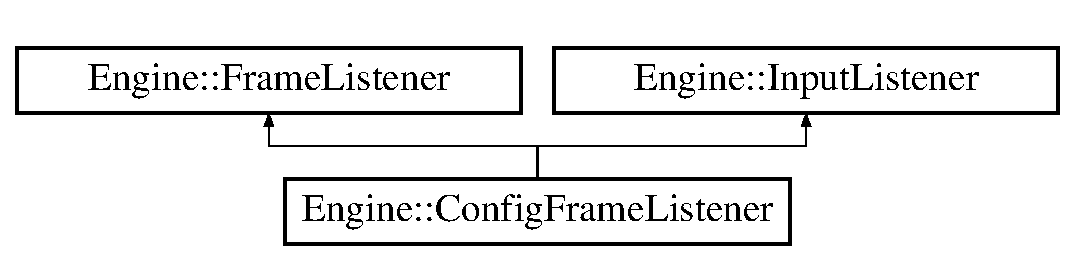
\includegraphics[height=2.000000cm]{classEngine_1_1ConfigFrameListener}
\end{center}
\end{figure}
\subsection*{Public Member Functions}
\begin{DoxyCompactItemize}
\item 
\hypertarget{classEngine_1_1ConfigFrameListener_a71f1b03339aeb75dfd45fcc4ca11f92f}{}{\bfseries Config\+Frame\+Listener} (const std\+::string \&config\+\_\+file)\label{classEngine_1_1ConfigFrameListener_a71f1b03339aeb75dfd45fcc4ca11f92f}

\item 
void \hyperlink{classEngine_1_1ConfigFrameListener_a792fe9af553206a358bc888fdc43f2be}{initialize} (\hyperlink{classEngine_1_1OpenPolygonDisplay}{Open\+Polygon\+Display} $\ast$display)
\begin{DoxyCompactList}\small\item\em initialize \end{DoxyCompactList}\item 
void \hyperlink{classEngine_1_1ConfigFrameListener_addb569607e5f870efda08a1a7de41544}{Render\+Logic} (float time)
\begin{DoxyCompactList}\small\item\em Render\+Logic. \end{DoxyCompactList}\item 
void \hyperlink{classEngine_1_1ConfigFrameListener_a2e412a7541868de93953c7cd818a6968}{on\+Key\+Event} (const \hyperlink{classEngine_1_1KeyEvent}{Key\+Event} \&event)
\begin{DoxyCompactList}\small\item\em on\+Key\+Event \end{DoxyCompactList}\item 
void \hyperlink{classEngine_1_1ConfigFrameListener_ac293a2b4c841a19e39d5e3d74eeb6ec3}{on\+Mouse\+Event} (const \hyperlink{classEngine_1_1MouseEvent}{Mouse\+Event} \&event)
\begin{DoxyCompactList}\small\item\em on\+Mouse\+Event \end{DoxyCompactList}\end{DoxyCompactItemize}
\subsection*{Protected Member Functions}
\begin{DoxyCompactItemize}
\item 
\hypertarget{classEngine_1_1ConfigFrameListener_ae8c208fbe77a97c8d9a7a82ff080e92e}{}void {\bfseries create\+Overlay} (void)\label{classEngine_1_1ConfigFrameListener_ae8c208fbe77a97c8d9a7a82ff080e92e}

\item 
\hypertarget{classEngine_1_1ConfigFrameListener_ae33859ce089cb5f4bc55d3b77bafc125}{}void {\bfseries create\+System} (\hyperlink{classEngine_1_1OpenPolygonDisplay}{Open\+Polygon\+Display} $\ast$display)\label{classEngine_1_1ConfigFrameListener_ae33859ce089cb5f4bc55d3b77bafc125}

\item 
\hypertarget{classEngine_1_1ConfigFrameListener_a52771ab4b5de16c06ce8f98b144308b7}{}void {\bfseries Show\+F\+P\+S} (float time)\label{classEngine_1_1ConfigFrameListener_a52771ab4b5de16c06ce8f98b144308b7}

\item 
\hypertarget{classEngine_1_1ConfigFrameListener_ac60e760b67dbff85a529bb86d3debc15}{}void {\bfseries Destroy\+Window} (const \hyperlink{classEngine_1_1KeyEvent}{Key\+Event} \&event)\label{classEngine_1_1ConfigFrameListener_ac60e760b67dbff85a529bb86d3debc15}

\item 
\hypertarget{classEngine_1_1ConfigFrameListener_a2511ac77cfa18011d978f3223cb2a59a}{}void {\bfseries Mouse\+Panel\+Collision} (void)\label{classEngine_1_1ConfigFrameListener_a2511ac77cfa18011d978f3223cb2a59a}

\end{DoxyCompactItemize}


\subsection{Detailed Description}
The \hyperlink{classEngine_1_1ConfigFrameListener}{Config\+Frame\+Listener} class. 

\subsection{Member Function Documentation}
\hypertarget{classEngine_1_1ConfigFrameListener_a792fe9af553206a358bc888fdc43f2be}{}\index{Engine\+::\+Config\+Frame\+Listener@{Engine\+::\+Config\+Frame\+Listener}!initialize@{initialize}}
\index{initialize@{initialize}!Engine\+::\+Config\+Frame\+Listener@{Engine\+::\+Config\+Frame\+Listener}}
\subsubsection[{initialize(\+Open\+Polygon\+Display $\ast$display)}]{\setlength{\rightskip}{0pt plus 5cm}void Config\+Frame\+Listener\+::initialize (
\begin{DoxyParamCaption}
\item[{{\bf Open\+Polygon\+Display} $\ast$}]{display}
\end{DoxyParamCaption}
)\hspace{0.3cm}{\ttfamily [virtual]}}\label{classEngine_1_1ConfigFrameListener_a792fe9af553206a358bc888fdc43f2be}


initialize 

Initialize Part


\begin{DoxyItemize}
\item create Elements or \hyperlink{classEngine_1_1Entity}{Entity} Objects
\item create a Scene 
\end{DoxyItemize}

Implements \hyperlink{classEngine_1_1FrameListener_abbe0d745faf156e01d2317b52f29bb48}{Engine\+::\+Frame\+Listener}.

\hypertarget{classEngine_1_1ConfigFrameListener_a2e412a7541868de93953c7cd818a6968}{}\index{Engine\+::\+Config\+Frame\+Listener@{Engine\+::\+Config\+Frame\+Listener}!on\+Key\+Event@{on\+Key\+Event}}
\index{on\+Key\+Event@{on\+Key\+Event}!Engine\+::\+Config\+Frame\+Listener@{Engine\+::\+Config\+Frame\+Listener}}
\subsubsection[{on\+Key\+Event(const Key\+Event \&event)}]{\setlength{\rightskip}{0pt plus 5cm}void Config\+Frame\+Listener\+::on\+Key\+Event (
\begin{DoxyParamCaption}
\item[{const {\bf Key\+Event} \&}]{event}
\end{DoxyParamCaption}
)\hspace{0.3cm}{\ttfamily [virtual]}}\label{classEngine_1_1ConfigFrameListener_a2e412a7541868de93953c7cd818a6968}


on\+Key\+Event 

Catch a Keyboard Event 
\begin{DoxyParams}{Parameters}
{\em event} & \\
\hline
\end{DoxyParams}


Implements \hyperlink{classEngine_1_1InputListener_abcd5e74a03230108bf29f68f74c1a878}{Engine\+::\+Input\+Listener}.

\hypertarget{classEngine_1_1ConfigFrameListener_ac293a2b4c841a19e39d5e3d74eeb6ec3}{}\index{Engine\+::\+Config\+Frame\+Listener@{Engine\+::\+Config\+Frame\+Listener}!on\+Mouse\+Event@{on\+Mouse\+Event}}
\index{on\+Mouse\+Event@{on\+Mouse\+Event}!Engine\+::\+Config\+Frame\+Listener@{Engine\+::\+Config\+Frame\+Listener}}
\subsubsection[{on\+Mouse\+Event(const Mouse\+Event \&event)}]{\setlength{\rightskip}{0pt plus 5cm}void Config\+Frame\+Listener\+::on\+Mouse\+Event (
\begin{DoxyParamCaption}
\item[{const {\bf Mouse\+Event} \&}]{event}
\end{DoxyParamCaption}
)\hspace{0.3cm}{\ttfamily [virtual]}}\label{classEngine_1_1ConfigFrameListener_ac293a2b4c841a19e39d5e3d74eeb6ec3}


on\+Mouse\+Event 

Catch a Mouse Event 
\begin{DoxyParams}{Parameters}
{\em event} & \\
\hline
\end{DoxyParams}


Implements \hyperlink{classEngine_1_1InputListener_aeee4d9f56950838b71d17ece61656736}{Engine\+::\+Input\+Listener}.

\hypertarget{classEngine_1_1ConfigFrameListener_addb569607e5f870efda08a1a7de41544}{}\index{Engine\+::\+Config\+Frame\+Listener@{Engine\+::\+Config\+Frame\+Listener}!Render\+Logic@{Render\+Logic}}
\index{Render\+Logic@{Render\+Logic}!Engine\+::\+Config\+Frame\+Listener@{Engine\+::\+Config\+Frame\+Listener}}
\subsubsection[{Render\+Logic(float time)}]{\setlength{\rightskip}{0pt plus 5cm}void Config\+Frame\+Listener\+::\+Render\+Logic (
\begin{DoxyParamCaption}
\item[{float}]{time}
\end{DoxyParamCaption}
)\hspace{0.3cm}{\ttfamily [virtual]}}\label{classEngine_1_1ConfigFrameListener_addb569607e5f870efda08a1a7de41544}


Render\+Logic. 

Logic Part


\begin{DoxyItemize}
\item modifier Elements or Entitys
\end{DoxyItemize}


\begin{DoxyParams}{Parameters}
{\em time} & \\
\hline
\end{DoxyParams}


Implements \hyperlink{classEngine_1_1FrameListener_a3e111a872dd6592c14e11d3280ce14c4}{Engine\+::\+Frame\+Listener}.



The documentation for this class was generated from the following files\+:\begin{DoxyCompactItemize}
\item 
include/\+Config/configframelistener.\+h\item 
Container/\+Config/Config\+Frame\+Listener.\+cpp\end{DoxyCompactItemize}

\hypertarget{classEngine_1_1ConfigManager}{}\section{Engine\+:\+:Config\+Manager Class Reference}
\label{classEngine_1_1ConfigManager}\index{Engine\+::\+Config\+Manager@{Engine\+::\+Config\+Manager}}
\subsection*{Public Member Functions}
\begin{DoxyCompactItemize}
\item 
\hypertarget{classEngine_1_1ConfigManager_a95118749dd2f38829ee09a6eb90f70e2}{}\hyperlink{classEngine_1_1Config}{Config} $\ast$ {\bfseries create\+Config} (const std\+::string \&file\+\_\+name)\label{classEngine_1_1ConfigManager_a95118749dd2f38829ee09a6eb90f70e2}

\item 
\hypertarget{classEngine_1_1ConfigManager_a98fc96995f335b6134ab2cb3a6178997}{}void {\bfseries add\+Function} (\hyperlink{classEngine_1_1Config}{Config} $\ast$config, const std\+::string \&value, C\+O\+N\+F\+I\+G\+\_\+\+F\+U\+N\+C func)\label{classEngine_1_1ConfigManager_a98fc96995f335b6134ab2cb3a6178997}

\item 
\hypertarget{classEngine_1_1ConfigManager_af2eb3430ee5ad83d772d6bfbe3745f54}{}void {\bfseries load\+Config} (\hyperlink{classEngine_1_1Config}{Config} $\ast$config)\label{classEngine_1_1ConfigManager_af2eb3430ee5ad83d772d6bfbe3745f54}

\item 
\hypertarget{classEngine_1_1ConfigManager_ac27f74f7d9f15a9b6454c710fc595cb7}{}\hyperlink{classEngine_1_1Config}{Config} $\ast$ {\bfseries get\+Config} (const std\+::string \&file\+\_\+name)\label{classEngine_1_1ConfigManager_ac27f74f7d9f15a9b6454c710fc595cb7}

\item 
\hypertarget{classEngine_1_1ConfigManager_a80a1a3ceaa64a0de6b469b7692351e21}{}void {\bfseries save\+Config} (\hyperlink{classEngine_1_1Config}{Config} $\ast$config)\label{classEngine_1_1ConfigManager_a80a1a3ceaa64a0de6b469b7692351e21}

\item 
\hypertarget{classEngine_1_1ConfigManager_a2aaa3562ee59c501b6d8b9be51275c32}{}void {\bfseries remove\+Config} (\hyperlink{classEngine_1_1Config}{Config} $\ast$config)\label{classEngine_1_1ConfigManager_a2aaa3562ee59c501b6d8b9be51275c32}

\item 
\hypertarget{classEngine_1_1ConfigManager_a9c732aeabdb06db0f9079646bf579144}{}void {\bfseries remove\+All} (void)\label{classEngine_1_1ConfigManager_a9c732aeabdb06db0f9079646bf579144}

\end{DoxyCompactItemize}
\subsection*{Static Public Member Functions}
\begin{DoxyCompactItemize}
\item 
\hypertarget{classEngine_1_1ConfigManager_ad5bf04a62c7b408a902a6a933b7ce7de}{}static \hyperlink{classEngine_1_1ConfigManager}{Config\+Manager} $\ast$ {\bfseries get\+Singelton\+Ptr} (void)\label{classEngine_1_1ConfigManager_ad5bf04a62c7b408a902a6a933b7ce7de}

\end{DoxyCompactItemize}


The documentation for this class was generated from the following files\+:\begin{DoxyCompactItemize}
\item 
include/\+Manager/configmanager.\+h\item 
Engine/\+Manager/Config\+Manager.\+cpp\end{DoxyCompactItemize}

\hypertarget{classEngine_1_1CubeMapping}{}\section{Engine\+:\+:Cube\+Mapping Class Reference}
\label{classEngine_1_1CubeMapping}\index{Engine\+::\+Cube\+Mapping@{Engine\+::\+Cube\+Mapping}}


The \hyperlink{classEngine_1_1CubeMapping}{Cube\+Mapping} class.  




{\ttfamily \#include $<$cubemapping.\+h$>$}

Inheritance diagram for Engine\+:\+:Cube\+Mapping\+:\begin{figure}[H]
\begin{center}
\leavevmode
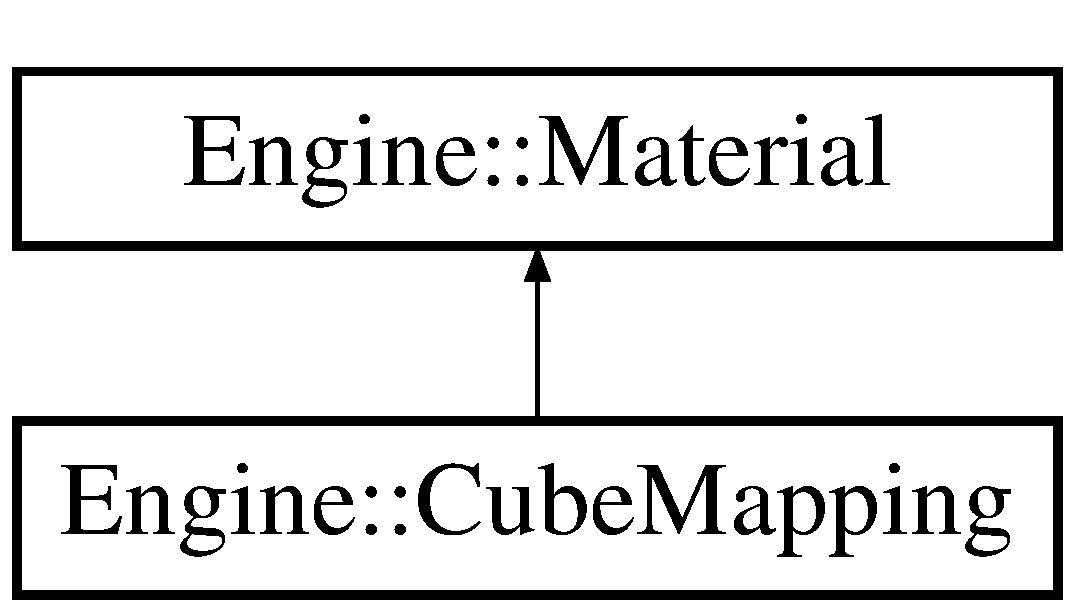
\includegraphics[height=2.000000cm]{classEngine_1_1CubeMapping}
\end{center}
\end{figure}
\subsection*{Public Member Functions}
\begin{DoxyCompactItemize}
\item 
\hypertarget{classEngine_1_1CubeMapping_abe5d082c7149004faf7fb15503805770}{}{\bfseries Cube\+Mapping} (\hyperlink{classEngine_1_1Entity}{Entity} $\ast$entity)\label{classEngine_1_1CubeMapping_abe5d082c7149004faf7fb15503805770}

\item 
\hypertarget{classEngine_1_1CubeMapping_aae33bd91f464a7ecef5c22d598e9da50}{}void {\bfseries create} (Textures textures, const string \&cube\+\_\+name)\label{classEngine_1_1CubeMapping_aae33bd91f464a7ecef5c22d598e9da50}

\item 
\hypertarget{classEngine_1_1CubeMapping_a8dec1352f578bcdc470b4c468c216624}{}void {\bfseries enable} (int texture\+\_\+unit)\label{classEngine_1_1CubeMapping_a8dec1352f578bcdc470b4c468c216624}

\end{DoxyCompactItemize}
\subsection*{Additional Inherited Members}


\subsection{Detailed Description}
The \hyperlink{classEngine_1_1CubeMapping}{Cube\+Mapping} class. 

The documentation for this class was generated from the following files\+:\begin{DoxyCompactItemize}
\item 
include/\+Material/cubemapping.\+h\item 
Container/\+Material/Cubemapping.\+cpp\end{DoxyCompactItemize}

\hypertarget{classEngine_1_1CustomThreadClass}{}\section{Engine\+:\+:Custom\+Thread\+Class Class Reference}
\label{classEngine_1_1CustomThreadClass}\index{Engine\+::\+Custom\+Thread\+Class@{Engine\+::\+Custom\+Thread\+Class}}


The documentation for this class was generated from the following file\+:\begin{DoxyCompactItemize}
\item 
include/\+Manager/threadmanager.\+h\end{DoxyCompactItemize}

\hypertarget{classEngine_1_1DisplayConfig}{}\section{Engine\+:\+:Display\+Config Class Reference}
\label{classEngine_1_1DisplayConfig}\index{Engine\+::\+Display\+Config@{Engine\+::\+Display\+Config}}


The \hyperlink{classEngine_1_1DisplayConfig}{Display\+Config} -\/ config class.  




{\ttfamily \#include $<$displayconfig.\+h$>$}

Inheritance diagram for Engine\+:\+:Display\+Config\+:\begin{figure}[H]
\begin{center}
\leavevmode
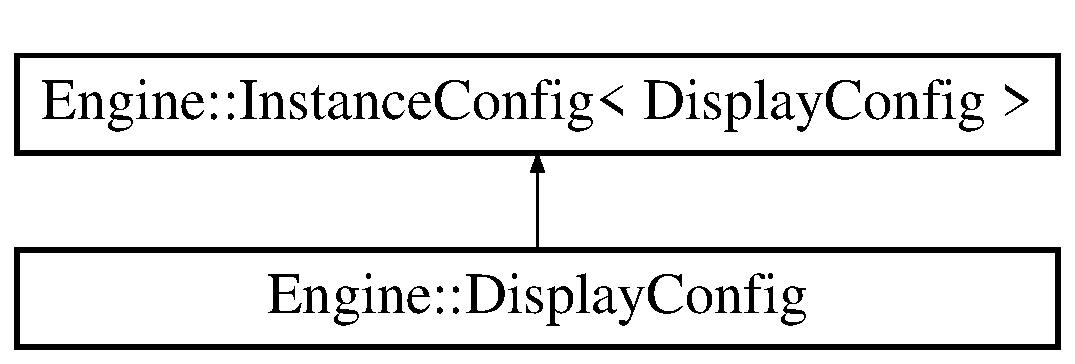
\includegraphics[height=2.000000cm]{classEngine_1_1DisplayConfig}
\end{center}
\end{figure}
\subsection*{Public Member Functions}
\begin{DoxyCompactItemize}
\item 
\hypertarget{classEngine_1_1DisplayConfig_a4e7905d09707c35596fd22707136588c}{}{\bfseries Display\+Config} (const std\+::string \&file\+\_\+name)\label{classEngine_1_1DisplayConfig_a4e7905d09707c35596fd22707136588c}

\item 
\hypertarget{classEngine_1_1DisplayConfig_abfa0fcd8c66497fe43f82dfdd2d2a4ae}{}void {\bfseries initialize} (void)\label{classEngine_1_1DisplayConfig_abfa0fcd8c66497fe43f82dfdd2d2a4ae}

\item 
\hypertarget{classEngine_1_1DisplayConfig_aa2901260dd6c24342ccee37412329e89}{}void {\bfseries read\+\_\+title} (const std\+::string \&content)\label{classEngine_1_1DisplayConfig_aa2901260dd6c24342ccee37412329e89}

\item 
\hypertarget{classEngine_1_1DisplayConfig_a8edf7a9d4f69fd5e84ac119b3f2b810c}{}void {\bfseries read\+\_\+windowsize} (const std\+::string \&content)\label{classEngine_1_1DisplayConfig_a8edf7a9d4f69fd5e84ac119b3f2b810c}

\item 
\hypertarget{classEngine_1_1DisplayConfig_a7bede44f27d1d00d1c9a2602600968c6}{}void {\bfseries read\+\_\+msaa} (const std\+::string \&content)\label{classEngine_1_1DisplayConfig_a7bede44f27d1d00d1c9a2602600968c6}

\item 
\hypertarget{classEngine_1_1DisplayConfig_ab6d633f0f8ac95853e197f9de2a5c048}{}void {\bfseries read\+\_\+context\+\_\+major} (const std\+::string \&content)\label{classEngine_1_1DisplayConfig_ab6d633f0f8ac95853e197f9de2a5c048}

\item 
\hypertarget{classEngine_1_1DisplayConfig_a8554ad75b0565963c3fd2994dd7665cf}{}void {\bfseries read\+\_\+context\+\_\+minor} (const std\+::string \&content)\label{classEngine_1_1DisplayConfig_a8554ad75b0565963c3fd2994dd7665cf}

\item 
\hypertarget{classEngine_1_1DisplayConfig_a844f9dcada077280c7e1d1b814138446}{}void {\bfseries read\+\_\+vsync} (const std\+::string \&content)\label{classEngine_1_1DisplayConfig_a844f9dcada077280c7e1d1b814138446}

\item 
\hypertarget{classEngine_1_1DisplayConfig_a2198b47c51f453ec77cc6040bc7e07f0}{}void {\bfseries read\+\_\+perspective} (const std\+::string \&content)\label{classEngine_1_1DisplayConfig_a2198b47c51f453ec77cc6040bc7e07f0}

\end{DoxyCompactItemize}
\subsection*{Public Attributes}
\begin{DoxyCompactItemize}
\item 
\hypertarget{classEngine_1_1DisplayConfig_a2f9c108805bb090aa22b293199ad9f6a}{}string {\bfseries m\+Title}\label{classEngine_1_1DisplayConfig_a2f9c108805bb090aa22b293199ad9f6a}

\item 
\hypertarget{classEngine_1_1DisplayConfig_a13246eda30c6f050914c5ee8301eba8b}{}glm\+::mat4 {\bfseries m\+Perspective}\label{classEngine_1_1DisplayConfig_a13246eda30c6f050914c5ee8301eba8b}

\item 
\hypertarget{classEngine_1_1DisplayConfig_a3658be3a503df4de4215dd64af446a0c}{}int {\bfseries m\+Width}\label{classEngine_1_1DisplayConfig_a3658be3a503df4de4215dd64af446a0c}

\item 
\hypertarget{classEngine_1_1DisplayConfig_ae46440a8edd4c96839219927f61af515}{}int {\bfseries m\+Height}\label{classEngine_1_1DisplayConfig_ae46440a8edd4c96839219927f61af515}

\item 
\hypertarget{classEngine_1_1DisplayConfig_ad699df2a2aee0e6a56ac7860f8abc8cb}{}int {\bfseries m\+M\+S\+A\+A}\label{classEngine_1_1DisplayConfig_ad699df2a2aee0e6a56ac7860f8abc8cb}

\item 
\hypertarget{classEngine_1_1DisplayConfig_ad71c9629be0b5955cd69a2c05060de71}{}int {\bfseries m\+Context\+\_\+major}\label{classEngine_1_1DisplayConfig_ad71c9629be0b5955cd69a2c05060de71}

\item 
\hypertarget{classEngine_1_1DisplayConfig_ad17ce18665c07b8378267ff30f3496be}{}int {\bfseries m\+Context\+\_\+minor}\label{classEngine_1_1DisplayConfig_ad17ce18665c07b8378267ff30f3496be}

\item 
\hypertarget{classEngine_1_1DisplayConfig_a2d1cbd250b87d43fb169ae005c8ebafa}{}int {\bfseries m\+V\+S\+Y\+N\+C}\label{classEngine_1_1DisplayConfig_a2d1cbd250b87d43fb169ae005c8ebafa}

\end{DoxyCompactItemize}
\subsection*{Additional Inherited Members}


\subsection{Detailed Description}
The \hyperlink{classEngine_1_1DisplayConfig}{Display\+Config} -\/ config class. 

The documentation for this class was generated from the following files\+:\begin{DoxyCompactItemize}
\item 
include/\+Config/displayconfig.\+h\item 
Container/\+Config/Display\+Config.\+cpp\end{DoxyCompactItemize}

\hypertarget{structEngine_1_1DisplayData}{}\section{Engine\+:\+:Display\+Data Struct Reference}
\label{structEngine_1_1DisplayData}\index{Engine\+::\+Display\+Data@{Engine\+::\+Display\+Data}}


The \hyperlink{structEngine_1_1DisplayData}{Display\+Data} struct.  




{\ttfamily \#include $<$display.\+h$>$}

\subsection*{Public Attributes}
\begin{DoxyCompactItemize}
\item 
\hypertarget{structEngine_1_1DisplayData_a576186911802decb15a7f73fb80a760f}{}int {\bfseries width}\label{structEngine_1_1DisplayData_a576186911802decb15a7f73fb80a760f}

\item 
\hypertarget{structEngine_1_1DisplayData_a8be5c86e7a59c5213f80d725531201ae}{}int {\bfseries height}\label{structEngine_1_1DisplayData_a8be5c86e7a59c5213f80d725531201ae}

\item 
\hypertarget{structEngine_1_1DisplayData_a90c689d6b5664922ca78045a34392164}{}int {\bfseries viewport\+\_\+x}\label{structEngine_1_1DisplayData_a90c689d6b5664922ca78045a34392164}

\item 
\hypertarget{structEngine_1_1DisplayData_abd6b90c1e0388736978e9c52d146d64b}{}int {\bfseries viewport\+\_\+y}\label{structEngine_1_1DisplayData_abd6b90c1e0388736978e9c52d146d64b}

\item 
\hypertarget{structEngine_1_1DisplayData_afd11e145d90e7d2c2b9b2bc25dc8e327}{}const char $\ast$ {\bfseries title}\label{structEngine_1_1DisplayData_afd11e145d90e7d2c2b9b2bc25dc8e327}

\item 
\hypertarget{structEngine_1_1DisplayData_a74c2d2098859902e1c09de3c26cbc2aa}{}std\+::string {\bfseries name}\label{structEngine_1_1DisplayData_a74c2d2098859902e1c09de3c26cbc2aa}

\item 
\hypertarget{structEngine_1_1DisplayData_a3aa8443a4b2aab960c6ce44413a9ebd4}{}glm\+::mat4 {\bfseries perspective}\label{structEngine_1_1DisplayData_a3aa8443a4b2aab960c6ce44413a9ebd4}

\end{DoxyCompactItemize}


\subsection{Detailed Description}
The \hyperlink{structEngine_1_1DisplayData}{Display\+Data} struct. 

The documentation for this struct was generated from the following file\+:\begin{DoxyCompactItemize}
\item 
include/\+Container/display.\+h\end{DoxyCompactItemize}

\hypertarget{classEngine_1_1DisplayManager}{}\section{Engine\+:\+:Display\+Manager Class Reference}
\label{classEngine_1_1DisplayManager}\index{Engine\+::\+Display\+Manager@{Engine\+::\+Display\+Manager}}


The \hyperlink{classEngine_1_1DisplayManager}{Display\+Manager} controlled the G\+L\+F\+W Display.  




{\ttfamily \#include $<$displaymanager.\+h$>$}

\subsection*{Public Member Functions}
\begin{DoxyCompactItemize}
\item 
void \hyperlink{classEngine_1_1DisplayManager_a2034225de0736f0e744ea1505f64077f}{initialize} (\hyperlink{classEngine_1_1DisplayConfig}{Display\+Config} $\ast$config)
\begin{DoxyCompactList}\small\item\em initialize \end{DoxyCompactList}\item 
\hypertarget{classEngine_1_1DisplayManager_afad79bba02480072eaf9fdf88f7e0172}{}void {\bfseries finish} (void)\label{classEngine_1_1DisplayManager_afad79bba02480072eaf9fdf88f7e0172}

\item 
\hypertarget{classEngine_1_1DisplayManager_a1bc6ee2cd4083b18548bfaa33a95733f}{}\hyperlink{classEngine_1_1GLFWDisplay}{G\+L\+F\+W\+Display} $\ast$ {\bfseries get\+Display} (const std\+::string \&display\+\_\+name)\label{classEngine_1_1DisplayManager_a1bc6ee2cd4083b18548bfaa33a95733f}

\item 
\hyperlink{classEngine_1_1GLFWDisplay}{G\+L\+F\+W\+Display} $\ast$ \hyperlink{classEngine_1_1DisplayManager_ad305871cfad4010eac228d98336b4ebb}{create\+Display} (\hyperlink{classEngine_1_1DisplayConfig}{Display\+Config} $\ast$config)  throw ( std\+::runtime\+\_\+error )
\begin{DoxyCompactList}\small\item\em create\+Main\+Display \end{DoxyCompactList}\item 
\hyperlink{classEngine_1_1GLFWDisplay}{G\+L\+F\+W\+Display} $\ast$ \hyperlink{classEngine_1_1DisplayManager_a6e376561f7f70b69c5a31be76757f1ce}{create\+Display} (int width, int height, const char $\ast$window\+\_\+title, G\+L\+F\+Wwindow $\ast$share=N\+U\+L\+L)  throw ( std\+::runtime\+\_\+error )
\begin{DoxyCompactList}\small\item\em create\+Display \end{DoxyCompactList}\item 
void \hyperlink{classEngine_1_1DisplayManager_a1d91f6a00075812c852358d57670652a}{make\+Context} (\hyperlink{classEngine_1_1GLFWDisplay}{G\+L\+F\+W\+Display} $\ast$display)  throw ( std\+::runtime\+\_\+error )
\begin{DoxyCompactList}\small\item\em create\+Hide\+Display \end{DoxyCompactList}\item 
void \hyperlink{classEngine_1_1DisplayManager_ae8368c3ef80d8e19f793f2b7fecfe187}{Bind\+Callbacks\+To} (\hyperlink{classEngine_1_1GLFWDisplay}{G\+L\+F\+W\+Display} $\ast$display)  throw ( std\+::runtime\+\_\+error )
\begin{DoxyCompactList}\small\item\em Bind\+Callbacks\+To. \end{DoxyCompactList}\item 
Display\+List \hyperlink{classEngine_1_1DisplayManager_ae808617945e1a4245e7c8c12188f7f04}{get\+Display\+List} (void)
\begin{DoxyCompactList}\small\item\em get\+Display\+List \end{DoxyCompactList}\item 
void \hyperlink{classEngine_1_1DisplayManager_ad0315041a819d4866e55e2948980b925}{register\+Display} (\hyperlink{classEngine_1_1GLFWDisplay}{G\+L\+F\+W\+Display} $\ast$display)
\begin{DoxyCompactList}\small\item\em register\+Display \end{DoxyCompactList}\item 
void \hyperlink{classEngine_1_1DisplayManager_aea08e9c79832bc02db95950010d9af32}{unregister} (\hyperlink{classEngine_1_1GLFWDisplay}{G\+L\+F\+W\+Display} $\ast$display)
\begin{DoxyCompactList}\small\item\em unregister \end{DoxyCompactList}\item 
void \hyperlink{classEngine_1_1DisplayManager_a83ea413274fab221c8573ddaad077993}{destroy} (\hyperlink{classEngine_1_1GLFWDisplay}{G\+L\+F\+W\+Display} $\ast$display)
\begin{DoxyCompactList}\small\item\em destroy \end{DoxyCompactList}\end{DoxyCompactItemize}
\subsection*{Static Public Member Functions}
\begin{DoxyCompactItemize}
\item 
\hypertarget{classEngine_1_1DisplayManager_ad459645eef8d2167c2aef8859333272d}{}static void {\bfseries Resize\+Callback} (G\+L\+F\+Wwindow $\ast$window, int width, int height)\label{classEngine_1_1DisplayManager_ad459645eef8d2167c2aef8859333272d}

\item 
\hypertarget{classEngine_1_1DisplayManager_a3585e07cfd3e567462413443ff56d1e7}{}static void {\bfseries Keyboard\+Callback} (G\+L\+F\+Wwindow $\ast$window, int key, int scancode, int action, int mods)\label{classEngine_1_1DisplayManager_a3585e07cfd3e567462413443ff56d1e7}

\item 
\hypertarget{classEngine_1_1DisplayManager_adc6a19826fcbc1e753fd9428e7025c03}{}static void {\bfseries Mouse\+Click\+Callback} (G\+L\+F\+Wwindow $\ast$window, int button, int action, int mods)\label{classEngine_1_1DisplayManager_adc6a19826fcbc1e753fd9428e7025c03}

\item 
\hypertarget{classEngine_1_1DisplayManager_a92ea0a3076a42c05c16f680ddbf53135}{}static void {\bfseries Cursor\+Callback} (G\+L\+F\+Wwindow $\ast$window, double x, double y)\label{classEngine_1_1DisplayManager_a92ea0a3076a42c05c16f680ddbf53135}

\item 
\hypertarget{classEngine_1_1DisplayManager_a013abbca377130d25261b5ce3a74e32c}{}static void {\bfseries Wheel\+Callback} (G\+L\+F\+Wwindow $\ast$window, double x, double y)\label{classEngine_1_1DisplayManager_a013abbca377130d25261b5ce3a74e32c}

\item 
static \hyperlink{classEngine_1_1DisplayManager}{Display\+Manager} $\ast$ \hyperlink{classEngine_1_1DisplayManager_ae8f1ed1758ca054854fd224496a80b29}{get\+Singleton\+Ptr} (void)
\begin{DoxyCompactList}\small\item\em get\+Singleton\+Ptr \end{DoxyCompactList}\end{DoxyCompactItemize}


\subsection{Detailed Description}
The \hyperlink{classEngine_1_1DisplayManager}{Display\+Manager} controlled the G\+L\+F\+W Display. 

\subsection{Member Function Documentation}
\hypertarget{classEngine_1_1DisplayManager_ae8368c3ef80d8e19f793f2b7fecfe187}{}\index{Engine\+::\+Display\+Manager@{Engine\+::\+Display\+Manager}!Bind\+Callbacks\+To@{Bind\+Callbacks\+To}}
\index{Bind\+Callbacks\+To@{Bind\+Callbacks\+To}!Engine\+::\+Display\+Manager@{Engine\+::\+Display\+Manager}}
\subsubsection[{Bind\+Callbacks\+To(\+G\+L\+F\+W\+Display $\ast$display)}]{\setlength{\rightskip}{0pt plus 5cm}void Display\+Manager\+::\+Bind\+Callbacks\+To (
\begin{DoxyParamCaption}
\item[{{\bf G\+L\+F\+W\+Display} $\ast$}]{display}
\end{DoxyParamCaption}
) throw  std\+::runtime\+\_\+error) }\label{classEngine_1_1DisplayManager_ae8368c3ef80d8e19f793f2b7fecfe187}


Bind\+Callbacks\+To. 

Bind all Callbacks to Display 
\begin{DoxyParams}{Parameters}
{\em display} & \\
\hline
\end{DoxyParams}
\hypertarget{classEngine_1_1DisplayManager_ad305871cfad4010eac228d98336b4ebb}{}\index{Engine\+::\+Display\+Manager@{Engine\+::\+Display\+Manager}!create\+Display@{create\+Display}}
\index{create\+Display@{create\+Display}!Engine\+::\+Display\+Manager@{Engine\+::\+Display\+Manager}}
\subsubsection[{create\+Display(\+Display\+Config $\ast$config)}]{\setlength{\rightskip}{0pt plus 5cm}{\bf G\+L\+F\+W\+Display} $\ast$ Display\+Manager\+::create\+Display (
\begin{DoxyParamCaption}
\item[{{\bf Display\+Config} $\ast$}]{config}
\end{DoxyParamCaption}
) throw  std\+::runtime\+\_\+error) }\label{classEngine_1_1DisplayManager_ad305871cfad4010eac228d98336b4ebb}


create\+Main\+Display 

Create Display by \hyperlink{classEngine_1_1DisplayConfig}{Display\+Config} 
\begin{DoxyParams}{Parameters}
{\em width} & \\
\hline
{\em height} & \\
\hline
{\em title} & \\
\hline
\end{DoxyParams}
\hypertarget{classEngine_1_1DisplayManager_a6e376561f7f70b69c5a31be76757f1ce}{}\index{Engine\+::\+Display\+Manager@{Engine\+::\+Display\+Manager}!create\+Display@{create\+Display}}
\index{create\+Display@{create\+Display}!Engine\+::\+Display\+Manager@{Engine\+::\+Display\+Manager}}
\subsubsection[{create\+Display(int width, int height, const char $\ast$window\+\_\+title, G\+L\+F\+Wwindow $\ast$share=\+N\+U\+L\+L)}]{\setlength{\rightskip}{0pt plus 5cm}{\bf G\+L\+F\+W\+Display} $\ast$ Display\+Manager\+::create\+Display (
\begin{DoxyParamCaption}
\item[{int}]{width, }
\item[{int}]{height, }
\item[{const char $\ast$}]{window\+\_\+title, }
\item[{G\+L\+F\+Wwindow $\ast$}]{share = {\ttfamily NULL}}
\end{DoxyParamCaption}
) throw  std\+::runtime\+\_\+error) }\label{classEngine_1_1DisplayManager_a6e376561f7f70b69c5a31be76757f1ce}


create\+Display 

Create G\+L\+F\+W Display 
\begin{DoxyParams}{Parameters}
{\em width} & \\
\hline
{\em height} & \\
\hline
{\em window\+\_\+title} & \\
\hline
\end{DoxyParams}
\begin{DoxyReturn}{Returns}

\end{DoxyReturn}
\hypertarget{classEngine_1_1DisplayManager_a83ea413274fab221c8573ddaad077993}{}\index{Engine\+::\+Display\+Manager@{Engine\+::\+Display\+Manager}!destroy@{destroy}}
\index{destroy@{destroy}!Engine\+::\+Display\+Manager@{Engine\+::\+Display\+Manager}}
\subsubsection[{destroy(\+G\+L\+F\+W\+Display $\ast$display)}]{\setlength{\rightskip}{0pt plus 5cm}void Display\+Manager\+::destroy (
\begin{DoxyParamCaption}
\item[{{\bf G\+L\+F\+W\+Display} $\ast$}]{display}
\end{DoxyParamCaption}
)}\label{classEngine_1_1DisplayManager_a83ea413274fab221c8573ddaad077993}


destroy 

Destroy a Display 
\begin{DoxyParams}{Parameters}
{\em display} & \\
\hline
\end{DoxyParams}
\hypertarget{classEngine_1_1DisplayManager_ae808617945e1a4245e7c8c12188f7f04}{}\index{Engine\+::\+Display\+Manager@{Engine\+::\+Display\+Manager}!get\+Display\+List@{get\+Display\+List}}
\index{get\+Display\+List@{get\+Display\+List}!Engine\+::\+Display\+Manager@{Engine\+::\+Display\+Manager}}
\subsubsection[{get\+Display\+List(void)}]{\setlength{\rightskip}{0pt plus 5cm}Display\+List Display\+Manager\+::get\+Display\+List (
\begin{DoxyParamCaption}
\item[{void}]{}
\end{DoxyParamCaption}
)}\label{classEngine_1_1DisplayManager_ae808617945e1a4245e7c8c12188f7f04}


get\+Display\+List 

Return all register displays \begin{DoxyReturn}{Returns}

\end{DoxyReturn}
\hypertarget{classEngine_1_1DisplayManager_ae8f1ed1758ca054854fd224496a80b29}{}\index{Engine\+::\+Display\+Manager@{Engine\+::\+Display\+Manager}!get\+Singleton\+Ptr@{get\+Singleton\+Ptr}}
\index{get\+Singleton\+Ptr@{get\+Singleton\+Ptr}!Engine\+::\+Display\+Manager@{Engine\+::\+Display\+Manager}}
\subsubsection[{get\+Singleton\+Ptr(void)}]{\setlength{\rightskip}{0pt plus 5cm}{\bf Display\+Manager} $\ast$ Display\+Manager\+::get\+Singleton\+Ptr (
\begin{DoxyParamCaption}
\item[{void}]{}
\end{DoxyParamCaption}
)\hspace{0.3cm}{\ttfamily [static]}}\label{classEngine_1_1DisplayManager_ae8f1ed1758ca054854fd224496a80b29}


get\+Singleton\+Ptr 

Return \hyperlink{classEngine_1_1Singleton}{Singleton} \hyperlink{classEngine_1_1DisplayManager}{Display\+Manager} Instance \begin{DoxyReturn}{Returns}

\end{DoxyReturn}
\hypertarget{classEngine_1_1DisplayManager_a2034225de0736f0e744ea1505f64077f}{}\index{Engine\+::\+Display\+Manager@{Engine\+::\+Display\+Manager}!initialize@{initialize}}
\index{initialize@{initialize}!Engine\+::\+Display\+Manager@{Engine\+::\+Display\+Manager}}
\subsubsection[{initialize(\+Display\+Config $\ast$config)}]{\setlength{\rightskip}{0pt plus 5cm}void Display\+Manager\+::initialize (
\begin{DoxyParamCaption}
\item[{{\bf Display\+Config} $\ast$}]{config}
\end{DoxyParamCaption}
)}\label{classEngine_1_1DisplayManager_a2034225de0736f0e744ea1505f64077f}


initialize 

Initialize G\+L\+F\+W 
\begin{DoxyParams}{Parameters}
{\em main\+\_\+display} & \\
\hline
\end{DoxyParams}
\hypertarget{classEngine_1_1DisplayManager_a1d91f6a00075812c852358d57670652a}{}\index{Engine\+::\+Display\+Manager@{Engine\+::\+Display\+Manager}!make\+Context@{make\+Context}}
\index{make\+Context@{make\+Context}!Engine\+::\+Display\+Manager@{Engine\+::\+Display\+Manager}}
\subsubsection[{make\+Context(\+G\+L\+F\+W\+Display $\ast$display)}]{\setlength{\rightskip}{0pt plus 5cm}void Display\+Manager\+::make\+Context (
\begin{DoxyParamCaption}
\item[{{\bf G\+L\+F\+W\+Display} $\ast$}]{display}
\end{DoxyParamCaption}
) throw  std\+::runtime\+\_\+error) }\label{classEngine_1_1DisplayManager_a1d91f6a00075812c852358d57670652a}


create\+Hide\+Display 

Create Hide G\+L\+F\+W Display \begin{DoxyReturn}{Returns}

\end{DoxyReturn}
G\+L\+F\+W -\/ Make Context


\begin{DoxyItemize}
\item \hyperlink{classEngine_1_1Thread}{Thread} Safety
\end{DoxyItemize}

make\+Context 
\begin{DoxyParams}{Parameters}
{\em display} & \\
\hline
\end{DoxyParams}
\hypertarget{classEngine_1_1DisplayManager_ad0315041a819d4866e55e2948980b925}{}\index{Engine\+::\+Display\+Manager@{Engine\+::\+Display\+Manager}!register\+Display@{register\+Display}}
\index{register\+Display@{register\+Display}!Engine\+::\+Display\+Manager@{Engine\+::\+Display\+Manager}}
\subsubsection[{register\+Display(\+G\+L\+F\+W\+Display $\ast$display)}]{\setlength{\rightskip}{0pt plus 5cm}void Display\+Manager\+::register\+Display (
\begin{DoxyParamCaption}
\item[{{\bf G\+L\+F\+W\+Display} $\ast$}]{display}
\end{DoxyParamCaption}
)}\label{classEngine_1_1DisplayManager_ad0315041a819d4866e55e2948980b925}


register\+Display 

register a display for more overview 
\begin{DoxyParams}{Parameters}
{\em display} & \\
\hline
\end{DoxyParams}
\hypertarget{classEngine_1_1DisplayManager_aea08e9c79832bc02db95950010d9af32}{}\index{Engine\+::\+Display\+Manager@{Engine\+::\+Display\+Manager}!unregister@{unregister}}
\index{unregister@{unregister}!Engine\+::\+Display\+Manager@{Engine\+::\+Display\+Manager}}
\subsubsection[{unregister(\+G\+L\+F\+W\+Display $\ast$display)}]{\setlength{\rightskip}{0pt plus 5cm}void Display\+Manager\+::unregister (
\begin{DoxyParamCaption}
\item[{{\bf G\+L\+F\+W\+Display} $\ast$}]{display}
\end{DoxyParamCaption}
)}\label{classEngine_1_1DisplayManager_aea08e9c79832bc02db95950010d9af32}


unregister 

remove a display from the display list


\begin{DoxyParams}{Parameters}
{\em display} & \\
\hline
\end{DoxyParams}


The documentation for this class was generated from the following files\+:\begin{DoxyCompactItemize}
\item 
include/\+Manager/displaymanager.\+h\item 
Engine/\+Manager/Display\+Manager.\+cpp\end{DoxyCompactItemize}

\hypertarget{structEngine_1_1DrawElementsCommand}{}\section{Engine\+:\+:Draw\+Elements\+Command Struct Reference}
\label{structEngine_1_1DrawElementsCommand}\index{Engine\+::\+Draw\+Elements\+Command@{Engine\+::\+Draw\+Elements\+Command}}


The \hyperlink{structEngine_1_1DrawElementsCommand}{Draw\+Elements\+Command} struct.  




{\ttfamily \#include $<$glvertexarrayobject.\+h$>$}

\subsection*{Public Attributes}
\begin{DoxyCompactItemize}
\item 
\hypertarget{structEngine_1_1DrawElementsCommand_a172930ac87063057bbd32e41ff191f03}{}G\+Luint {\bfseries vertex\+Count}\label{structEngine_1_1DrawElementsCommand_a172930ac87063057bbd32e41ff191f03}

\item 
\hypertarget{structEngine_1_1DrawElementsCommand_aecb2f3a602a00559404bc7cdce7d14da}{}G\+Luint {\bfseries instance\+Count}\label{structEngine_1_1DrawElementsCommand_aecb2f3a602a00559404bc7cdce7d14da}

\item 
\hypertarget{structEngine_1_1DrawElementsCommand_a75c7d73db84332530e4b0097e62f939f}{}G\+Luint {\bfseries first\+Index}\label{structEngine_1_1DrawElementsCommand_a75c7d73db84332530e4b0097e62f939f}

\item 
\hypertarget{structEngine_1_1DrawElementsCommand_ad07e7d6f304e0a71e41e2bd375888f6b}{}G\+Luint {\bfseries base\+Vertex}\label{structEngine_1_1DrawElementsCommand_ad07e7d6f304e0a71e41e2bd375888f6b}

\item 
\hypertarget{structEngine_1_1DrawElementsCommand_a500c4f20f38654ff58eafb3c34197999}{}G\+Luint {\bfseries base\+Instance}\label{structEngine_1_1DrawElementsCommand_a500c4f20f38654ff58eafb3c34197999}

\end{DoxyCompactItemize}


\subsection{Detailed Description}
The \hyperlink{structEngine_1_1DrawElementsCommand}{Draw\+Elements\+Command} struct. 

The documentation for this struct was generated from the following file\+:\begin{DoxyCompactItemize}
\item 
include/\+G\+P\+U/glvertexarrayobject.\+h\end{DoxyCompactItemize}

\hypertarget{classEngine_1_1DrawEvent}{}\section{Engine\+:\+:Draw\+Event Class Reference}
\label{classEngine_1_1DrawEvent}\index{Engine\+::\+Draw\+Event@{Engine\+::\+Draw\+Event}}


The \hyperlink{classEngine_1_1DrawEvent}{Draw\+Event} -\/ event class.  




{\ttfamily \#include $<$drawevent.\+h$>$}

\subsection*{Public Types}
\begin{DoxyCompactItemize}
\item 
\hypertarget{classEngine_1_1DrawEvent_ae318662b3a1237df5fab4d791e6fbe3b}{}enum {\bfseries M\+A\+T\+R\+I\+C\+E\+N} \{ {\bfseries P\+R\+O\+\_\+\+O\+R\+T\+H\+O}, 
{\bfseries P\+R\+O\+\_\+\+P\+R\+O\+J\+E\+C\+T\+I\+O\+N}, 
{\bfseries P\+R\+O\+\_\+\+U\+N\+K\+N\+O\+W\+N}
 \}\label{classEngine_1_1DrawEvent_ae318662b3a1237df5fab4d791e6fbe3b}

\end{DoxyCompactItemize}
\subsection*{Public Member Functions}
\begin{DoxyCompactItemize}
\item 
\hypertarget{classEngine_1_1DrawEvent_ac70cac77946442fa4f79f74097c3c1fb}{}void {\bfseries set\+Clip\+Distance} (const \hyperlink{classVector4}{Vector4f} \&clip\+\_\+distance)\label{classEngine_1_1DrawEvent_ac70cac77946442fa4f79f74097c3c1fb}

\item 
void \hyperlink{classEngine_1_1DrawEvent_adfcef67906c6b67390dfa83b92394d1a}{set\+Projection} (const glm\+::mat4 \&matrix, M\+A\+T\+R\+I\+C\+E\+N mode)
\begin{DoxyCompactList}\small\item\em set\+Projection \end{DoxyCompactList}\item 
void \hyperlink{classEngine_1_1DrawEvent_a59cf1065d97426947dcb92f4499b8c59}{set\+World\+View} (const glm\+::mat4 \&matrix)
\begin{DoxyCompactList}\small\item\em set\+World\+View \end{DoxyCompactList}\item 
void \hyperlink{classEngine_1_1DrawEvent_a4f6c4ed1ddda804cf905be74cbac909b}{set\+Model\+Matrix} (const glm\+::mat4 \&matrix)
\begin{DoxyCompactList}\small\item\em set\+Model\+View \end{DoxyCompactList}\item 
void \hyperlink{classEngine_1_1DrawEvent_a4fc992cab407a9e77ba4ad2ea85614d7}{set\+Texture} (const glm\+::mat4 \&matrix)
\begin{DoxyCompactList}\small\item\em set\+Texture \end{DoxyCompactList}\item 
void \hyperlink{classEngine_1_1DrawEvent_a496fa555d7762b2d0e6501fd5df6ecb5}{set\+Shadow} (const \hyperlink{classEngine_1_1ShadowEvent}{Shadow\+Event} \&event)
\begin{DoxyCompactList}\small\item\em set\+Shadow \end{DoxyCompactList}\item 
M\+A\+T\+R\+I\+C\+E\+N \hyperlink{classEngine_1_1DrawEvent_aeb66407c993f03211d133a5ddbd5ad6b}{get\+Projection\+Mode} (void) const 
\begin{DoxyCompactList}\small\item\em get\+Projection\+Mode \end{DoxyCompactList}\item 
\hypertarget{classEngine_1_1DrawEvent_aaaaa58ede3268870fb5542e35afb0b52}{}bool {\bfseries has\+Projection} (void) const \label{classEngine_1_1DrawEvent_aaaaa58ede3268870fb5542e35afb0b52}

\item 
\hypertarget{classEngine_1_1DrawEvent_a4c447f0dfeeb19b3f169811049d9ba58}{}bool {\bfseries has\+World\+View} (void) const \label{classEngine_1_1DrawEvent_a4c447f0dfeeb19b3f169811049d9ba58}

\item 
\hypertarget{classEngine_1_1DrawEvent_ae975d9472c0d02e6731ecd01a1327c09}{}bool {\bfseries has\+Model} (void) const \label{classEngine_1_1DrawEvent_ae975d9472c0d02e6731ecd01a1327c09}

\item 
\hypertarget{classEngine_1_1DrawEvent_a884ca99c31d79d5cd765a85bff3794b8}{}bool {\bfseries has\+Texture} (void) const \label{classEngine_1_1DrawEvent_a884ca99c31d79d5cd765a85bff3794b8}

\item 
\hypertarget{classEngine_1_1DrawEvent_a007fe111c202dae108bc562496e4ac16}{}bool {\bfseries has\+Shadow\+Event} (void) const \label{classEngine_1_1DrawEvent_a007fe111c202dae108bc562496e4ac16}

\item 
\hypertarget{classEngine_1_1DrawEvent_afc81c272b1e7e6c1adf3d5d3ee6adb63}{}glm\+::mat4 {\bfseries get\+Projection} (void) const \label{classEngine_1_1DrawEvent_afc81c272b1e7e6c1adf3d5d3ee6adb63}

\item 
\hypertarget{classEngine_1_1DrawEvent_a3d65f9a9295f26adf94ffc003de97212}{}glm\+::mat4 {\bfseries get\+World\+View} (void) const \label{classEngine_1_1DrawEvent_a3d65f9a9295f26adf94ffc003de97212}

\item 
\hypertarget{classEngine_1_1DrawEvent_a523c4294c0e1508221bbb5764632c84f}{}glm\+::mat4 {\bfseries get\+Model\+Matrix} (void) const \label{classEngine_1_1DrawEvent_a523c4294c0e1508221bbb5764632c84f}

\item 
\hypertarget{classEngine_1_1DrawEvent_af8d338da327a48180c5e03de0d938db6}{}glm\+::mat4 {\bfseries get\+Texture\+Matrix} (void) const \label{classEngine_1_1DrawEvent_af8d338da327a48180c5e03de0d938db6}

\item 
\hypertarget{classEngine_1_1DrawEvent_a7e677deb5c6903be0501da7bbee21dd2}{}const \hyperlink{classEngine_1_1ShadowEvent}{Shadow\+Event} {\bfseries get\+Shadow\+Event} (void) const \label{classEngine_1_1DrawEvent_a7e677deb5c6903be0501da7bbee21dd2}

\item 
\hypertarget{classEngine_1_1DrawEvent_adb6ff5576ad0b323cfe6fb6931ffa96d}{}const \hyperlink{classVector4}{Vector4f} {\bfseries get\+Clip\+Distance} (void) const \label{classEngine_1_1DrawEvent_adb6ff5576ad0b323cfe6fb6931ffa96d}

\end{DoxyCompactItemize}


\subsection{Detailed Description}
The \hyperlink{classEngine_1_1DrawEvent}{Draw\+Event} -\/ event class. 

\subsection{Member Function Documentation}
\hypertarget{classEngine_1_1DrawEvent_aeb66407c993f03211d133a5ddbd5ad6b}{}\index{Engine\+::\+Draw\+Event@{Engine\+::\+Draw\+Event}!get\+Projection\+Mode@{get\+Projection\+Mode}}
\index{get\+Projection\+Mode@{get\+Projection\+Mode}!Engine\+::\+Draw\+Event@{Engine\+::\+Draw\+Event}}
\subsubsection[{get\+Projection\+Mode(void) const }]{\setlength{\rightskip}{0pt plus 5cm}Draw\+Event\+::\+M\+A\+T\+R\+I\+C\+E\+N Draw\+Event\+::get\+Projection\+Mode (
\begin{DoxyParamCaption}
\item[{void}]{}
\end{DoxyParamCaption}
) const}\label{classEngine_1_1DrawEvent_aeb66407c993f03211d133a5ddbd5ad6b}


get\+Projection\+Mode 

Return the current Projection Mode if Projection Matrix is set \begin{DoxyReturn}{Returns}

\end{DoxyReturn}
\hypertarget{classEngine_1_1DrawEvent_a4f6c4ed1ddda804cf905be74cbac909b}{}\index{Engine\+::\+Draw\+Event@{Engine\+::\+Draw\+Event}!set\+Model\+Matrix@{set\+Model\+Matrix}}
\index{set\+Model\+Matrix@{set\+Model\+Matrix}!Engine\+::\+Draw\+Event@{Engine\+::\+Draw\+Event}}
\subsubsection[{set\+Model\+Matrix(const glm\+::mat4 \&matrix)}]{\setlength{\rightskip}{0pt plus 5cm}void Draw\+Event\+::set\+Model\+Matrix (
\begin{DoxyParamCaption}
\item[{const glm\+::mat4 \&}]{matrix}
\end{DoxyParamCaption}
)}\label{classEngine_1_1DrawEvent_a4f6c4ed1ddda804cf905be74cbac909b}


set\+Model\+View 

Model\+Matrix -\/$>$ Model\+Matrix is a Object Matrix ( example\+: light matrix ) 
\begin{DoxyParams}{Parameters}
{\em matrix} & \\
\hline
\end{DoxyParams}
\hypertarget{classEngine_1_1DrawEvent_adfcef67906c6b67390dfa83b92394d1a}{}\index{Engine\+::\+Draw\+Event@{Engine\+::\+Draw\+Event}!set\+Projection@{set\+Projection}}
\index{set\+Projection@{set\+Projection}!Engine\+::\+Draw\+Event@{Engine\+::\+Draw\+Event}}
\subsubsection[{set\+Projection(const glm\+::mat4 \&matrix, M\+A\+T\+R\+I\+C\+E\+N mode)}]{\setlength{\rightskip}{0pt plus 5cm}void Draw\+Event\+::set\+Projection (
\begin{DoxyParamCaption}
\item[{const glm\+::mat4 \&}]{matrix, }
\item[{M\+A\+T\+R\+I\+C\+E\+N}]{mode}
\end{DoxyParamCaption}
)}\label{classEngine_1_1DrawEvent_adfcef67906c6b67390dfa83b92394d1a}


set\+Projection 

Projection Matrix -\/ -\/$>$ ortho(2\+D) or projection(3\+D) 
\begin{DoxyParams}{Parameters}
{\em matrix} & \\
\hline
{\em mode} & \\
\hline
\end{DoxyParams}
\hypertarget{classEngine_1_1DrawEvent_a496fa555d7762b2d0e6501fd5df6ecb5}{}\index{Engine\+::\+Draw\+Event@{Engine\+::\+Draw\+Event}!set\+Shadow@{set\+Shadow}}
\index{set\+Shadow@{set\+Shadow}!Engine\+::\+Draw\+Event@{Engine\+::\+Draw\+Event}}
\subsubsection[{set\+Shadow(const Shadow\+Event \&event)}]{\setlength{\rightskip}{0pt plus 5cm}void Draw\+Event\+::set\+Shadow (
\begin{DoxyParamCaption}
\item[{const {\bf Shadow\+Event} \&}]{event}
\end{DoxyParamCaption}
)}\label{classEngine_1_1DrawEvent_a496fa555d7762b2d0e6501fd5df6ecb5}


set\+Shadow 

Set new Shadow Event 
\begin{DoxyParams}{Parameters}
{\em event} & \\
\hline
\end{DoxyParams}
\hypertarget{classEngine_1_1DrawEvent_a4fc992cab407a9e77ba4ad2ea85614d7}{}\index{Engine\+::\+Draw\+Event@{Engine\+::\+Draw\+Event}!set\+Texture@{set\+Texture}}
\index{set\+Texture@{set\+Texture}!Engine\+::\+Draw\+Event@{Engine\+::\+Draw\+Event}}
\subsubsection[{set\+Texture(const glm\+::mat4 \&matrix)}]{\setlength{\rightskip}{0pt plus 5cm}void Draw\+Event\+::set\+Texture (
\begin{DoxyParamCaption}
\item[{const glm\+::mat4 \&}]{matrix}
\end{DoxyParamCaption}
)}\label{classEngine_1_1DrawEvent_a4fc992cab407a9e77ba4ad2ea85614d7}


set\+Texture 

\hyperlink{classEngine_1_1Texture}{Texture} Matrix -\/ for \hyperlink{classEngine_1_1Texture}{Texture} Rotation $\vert$ Scaling


\begin{DoxyParams}{Parameters}
{\em matrix} & \\
\hline
\end{DoxyParams}
\hypertarget{classEngine_1_1DrawEvent_a59cf1065d97426947dcb92f4499b8c59}{}\index{Engine\+::\+Draw\+Event@{Engine\+::\+Draw\+Event}!set\+World\+View@{set\+World\+View}}
\index{set\+World\+View@{set\+World\+View}!Engine\+::\+Draw\+Event@{Engine\+::\+Draw\+Event}}
\subsubsection[{set\+World\+View(const glm\+::mat4 \&matrix)}]{\setlength{\rightskip}{0pt plus 5cm}void Draw\+Event\+::set\+World\+View (
\begin{DoxyParamCaption}
\item[{const glm\+::mat4 \&}]{matrix}
\end{DoxyParamCaption}
)}\label{classEngine_1_1DrawEvent_a59cf1065d97426947dcb92f4499b8c59}


set\+World\+View 

World\+View Matrix is the Camera\+Matrix or View\+Matrix 
\begin{DoxyParams}{Parameters}
{\em matrix} & \\
\hline
\end{DoxyParams}


The documentation for this class was generated from the following files\+:\begin{DoxyCompactItemize}
\item 
include/\+Container/drawevent.\+h\item 
Container/Draw\+Event.\+cpp\end{DoxyCompactItemize}

\hypertarget{structEngine_1_1EditorStore}{}\section{Engine\+:\+:Editor\+Store Struct Reference}
\label{structEngine_1_1EditorStore}\index{Engine\+::\+Editor\+Store@{Engine\+::\+Editor\+Store}}
\subsection*{Public Attributes}
\begin{DoxyCompactItemize}
\item 
\hypertarget{structEngine_1_1EditorStore_ae71310df3d29b539b288026be5736405}{}uint {\bfseries script\+\_\+mode}\label{structEngine_1_1EditorStore_ae71310df3d29b539b288026be5736405}

\item 
\hypertarget{structEngine_1_1EditorStore_a65b642e4ef92baffd8f0e72cae881ad6}{}uint {\bfseries draw\+\_\+mode}\label{structEngine_1_1EditorStore_a65b642e4ef92baffd8f0e72cae881ad6}

\item 
\hypertarget{structEngine_1_1EditorStore_ab5bc0c5d71b178fa3c4b46d59ddb1d3b}{}uint {\bfseries update\+\_\+mode}\label{structEngine_1_1EditorStore_ab5bc0c5d71b178fa3c4b46d59ddb1d3b}

\item 
\hypertarget{structEngine_1_1EditorStore_a8654bac30a30ac2f08cf2a76be13d6cb}{}uint {\bfseries shadow\+\_\+mode}\label{structEngine_1_1EditorStore_a8654bac30a30ac2f08cf2a76be13d6cb}

\item 
\hypertarget{structEngine_1_1EditorStore_a8c517f13358157dfe4f83c2bc2880416}{}uint {\bfseries texture\+\_\+mode}\label{structEngine_1_1EditorStore_a8c517f13358157dfe4f83c2bc2880416}

\item 
\hypertarget{structEngine_1_1EditorStore_a7273d42893d5c6499317ca35efdee9fc}{}int {\bfseries tbo\+\_\+draws}\label{structEngine_1_1EditorStore_a7273d42893d5c6499317ca35efdee9fc}

\item 
\hypertarget{structEngine_1_1EditorStore_abf2b21b2b7ef5e4376a4d7872f236eb4}{}string {\bfseries culling}\label{structEngine_1_1EditorStore_abf2b21b2b7ef5e4376a4d7872f236eb4}

\item 
\hypertarget{structEngine_1_1EditorStore_a86c12e4d7b5847bb7cf88b392fa6e0c1}{}Entity\+Object $\ast$ {\bfseries select}\label{structEngine_1_1EditorStore_a86c12e4d7b5847bb7cf88b392fa6e0c1}

\end{DoxyCompactItemize}


The documentation for this struct was generated from the following file\+:\begin{DoxyCompactItemize}
\item 
include/editorstore.\+h\end{DoxyCompactItemize}

\hypertarget{classEngine_1_1Element}{}\section{Engine\+:\+:Element Class Reference}
\label{classEngine_1_1Element}\index{Engine\+::\+Element@{Engine\+::\+Element}}


The \hyperlink{classEngine_1_1Element}{Element} -\/ base component class -\/ for 2\+D Entitys.  




{\ttfamily \#include $<$element.\+h$>$}

Inheritance diagram for Engine\+:\+:Element\+:\begin{figure}[H]
\begin{center}
\leavevmode
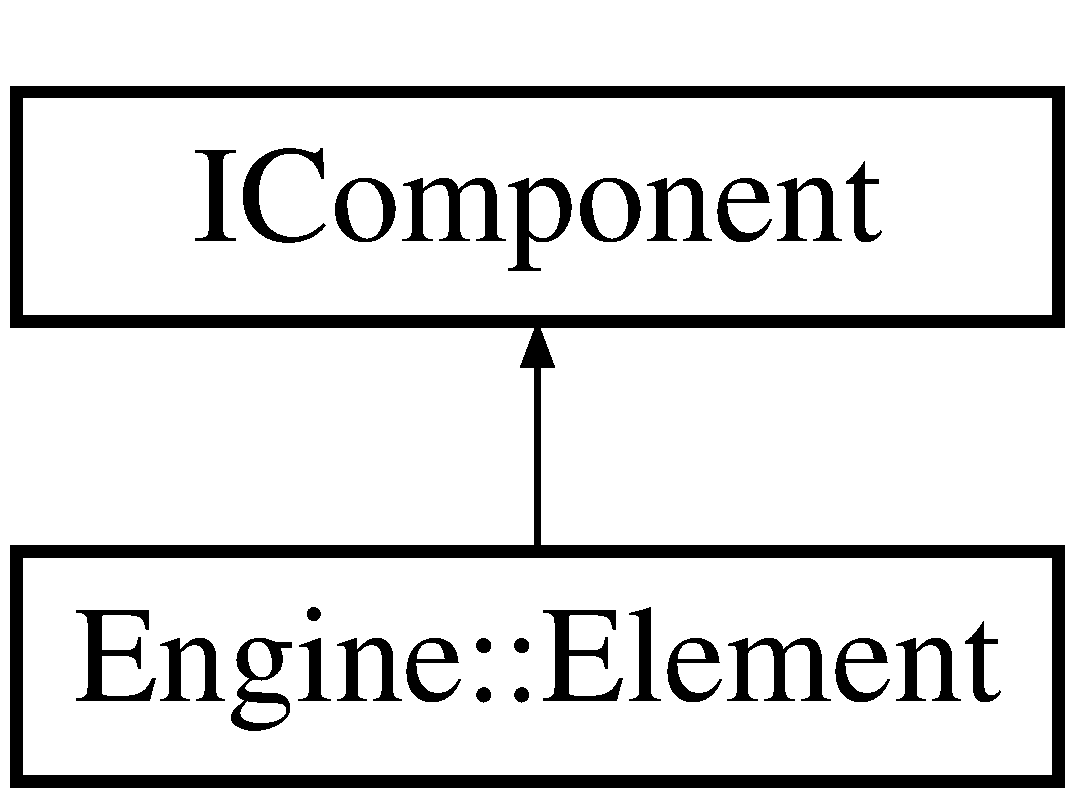
\includegraphics[height=2.000000cm]{classEngine_1_1Element}
\end{center}
\end{figure}
\subsection*{Public Member Functions}
\begin{DoxyCompactItemize}
\item 
uint \hyperlink{classEngine_1_1Element_a075b3f0f789c82b0f62444024ebc546d}{get\+Z\+Order} (void)
\begin{DoxyCompactList}\small\item\em get\+Z\+Order \end{DoxyCompactList}\item 
bool \hyperlink{classEngine_1_1Element_a143f4e6a395c96ee7f175e179272795b}{is\+Visible} (void)
\begin{DoxyCompactList}\small\item\em is\+Visible \end{DoxyCompactList}\item 
void \hyperlink{classEngine_1_1Element_a0cd1e777e57ac0717a0cdea484f66708}{set\+Visible} (bool)
\begin{DoxyCompactList}\small\item\em set\+Visible \end{DoxyCompactList}\item 
void \hyperlink{classEngine_1_1Element_aa43ecc291745829889ec923fe8d0ff76}{set\+Z\+Order} (int zorder)
\begin{DoxyCompactList}\small\item\em set\+Z\+Order \end{DoxyCompactList}\end{DoxyCompactItemize}


\subsection{Detailed Description}
The \hyperlink{classEngine_1_1Element}{Element} -\/ base component class -\/ for 2\+D Entitys. 

\subsection{Member Function Documentation}
\hypertarget{classEngine_1_1Element_a075b3f0f789c82b0f62444024ebc546d}{}\index{Engine\+::\+Element@{Engine\+::\+Element}!get\+Z\+Order@{get\+Z\+Order}}
\index{get\+Z\+Order@{get\+Z\+Order}!Engine\+::\+Element@{Engine\+::\+Element}}
\subsubsection[{get\+Z\+Order(void)}]{\setlength{\rightskip}{0pt plus 5cm}uint Element\+::get\+Z\+Order (
\begin{DoxyParamCaption}
\item[{void}]{}
\end{DoxyParamCaption}
)}\label{classEngine_1_1Element_a075b3f0f789c82b0f62444024ebc546d}


get\+Z\+Order 

Return Z Order \begin{DoxyReturn}{Returns}

\end{DoxyReturn}
\hypertarget{classEngine_1_1Element_a143f4e6a395c96ee7f175e179272795b}{}\index{Engine\+::\+Element@{Engine\+::\+Element}!is\+Visible@{is\+Visible}}
\index{is\+Visible@{is\+Visible}!Engine\+::\+Element@{Engine\+::\+Element}}
\subsubsection[{is\+Visible(void)}]{\setlength{\rightskip}{0pt plus 5cm}bool Element\+::is\+Visible (
\begin{DoxyParamCaption}
\item[{void}]{}
\end{DoxyParamCaption}
)}\label{classEngine_1_1Element_a143f4e6a395c96ee7f175e179272795b}


is\+Visible 

Return true -\/ if element is visible otherwise false \begin{DoxyReturn}{Returns}

\end{DoxyReturn}
\hypertarget{classEngine_1_1Element_a0cd1e777e57ac0717a0cdea484f66708}{}\index{Engine\+::\+Element@{Engine\+::\+Element}!set\+Visible@{set\+Visible}}
\index{set\+Visible@{set\+Visible}!Engine\+::\+Element@{Engine\+::\+Element}}
\subsubsection[{set\+Visible(bool)}]{\setlength{\rightskip}{0pt plus 5cm}void Element\+::set\+Visible (
\begin{DoxyParamCaption}
\item[{bool}]{visible}
\end{DoxyParamCaption}
)}\label{classEngine_1_1Element_a0cd1e777e57ac0717a0cdea484f66708}


set\+Visible 

Set visible state \hypertarget{classEngine_1_1Element_aa43ecc291745829889ec923fe8d0ff76}{}\index{Engine\+::\+Element@{Engine\+::\+Element}!set\+Z\+Order@{set\+Z\+Order}}
\index{set\+Z\+Order@{set\+Z\+Order}!Engine\+::\+Element@{Engine\+::\+Element}}
\subsubsection[{set\+Z\+Order(int zorder)}]{\setlength{\rightskip}{0pt plus 5cm}void Element\+::set\+Z\+Order (
\begin{DoxyParamCaption}
\item[{int}]{zorder}
\end{DoxyParamCaption}
)}\label{classEngine_1_1Element_aa43ecc291745829889ec923fe8d0ff76}


set\+Z\+Order 

Set zorder index 
\begin{DoxyParams}{Parameters}
{\em zorder} & \\
\hline
\end{DoxyParams}


The documentation for this class was generated from the following files\+:\begin{DoxyCompactItemize}
\item 
include/\+Component/element.\+h\item 
Component/Element.\+cpp\end{DoxyCompactItemize}

\hypertarget{classEngine_1_1ElementManager}{}\section{Engine\+:\+:Element\+Manager Class Reference}
\label{classEngine_1_1ElementManager}\index{Engine\+::\+Element\+Manager@{Engine\+::\+Element\+Manager}}


The \hyperlink{classEngine_1_1ElementManager}{Element\+Manager} controlled Elements ( are 2\+D Entitys )  




{\ttfamily \#include $<$elementmanager.\+h$>$}

Inheritance diagram for Engine\+:\+:Element\+Manager\+:\begin{figure}[H]
\begin{center}
\leavevmode
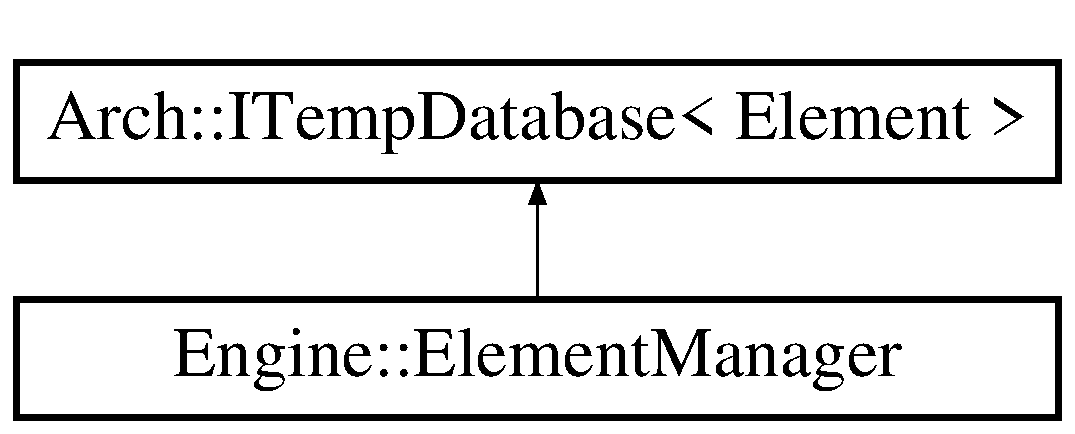
\includegraphics[height=2.000000cm]{classEngine_1_1ElementManager}
\end{center}
\end{figure}
\subsection*{Public Member Functions}
\begin{DoxyCompactItemize}
\item 
\hypertarget{classEngine_1_1ElementManager_ae5149303aa75cc787a4a48a46035c271}{}\hyperlink{classEngine_1_1Element}{Element} $\ast$ {\bfseries create\+Element} (void)\label{classEngine_1_1ElementManager_ae5149303aa75cc787a4a48a46035c271}

\item 
\hypertarget{classEngine_1_1ElementManager_a46404a987667a712fe45fbaf22637d8a}{}\hyperlink{classEngine_1_1Element}{Element} $\ast$ {\bfseries get\+Element} (uint container\+\_\+id)\label{classEngine_1_1ElementManager_a46404a987667a712fe45fbaf22637d8a}

\item 
\hypertarget{classEngine_1_1ElementManager_a2e6e82cca8c3c71c93619cf7c4e15e63}{}void {\bfseries destroy} (uint container\+\_\+id)\label{classEngine_1_1ElementManager_a2e6e82cca8c3c71c93619cf7c4e15e63}

\end{DoxyCompactItemize}


\subsection{Detailed Description}
The \hyperlink{classEngine_1_1ElementManager}{Element\+Manager} controlled Elements ( are 2\+D Entitys ) 

Componentv2 Database ( \hyperlink{classEngine_1_1ElementManager}{Element\+Manager} ) 

The documentation for this class was generated from the following files\+:\begin{DoxyCompactItemize}
\item 
include/\+Manager/elementmanager.\+h\item 
Engine/\+Manager/Element\+Manager.\+cpp\end{DoxyCompactItemize}

\hypertarget{classEngine_1_1Entity}{}\section{Engine\+:\+:Entity Class Reference}
\label{classEngine_1_1Entity}\index{Engine\+::\+Entity@{Engine\+::\+Entity}}


The \hyperlink{classEngine_1_1Entity}{Entity} -\/ base component class -\/ for 3\+D Entitys.  




{\ttfamily \#include $<$entity.\+h$>$}

Inheritance diagram for Engine\+:\+:Entity\+:\begin{figure}[H]
\begin{center}
\leavevmode
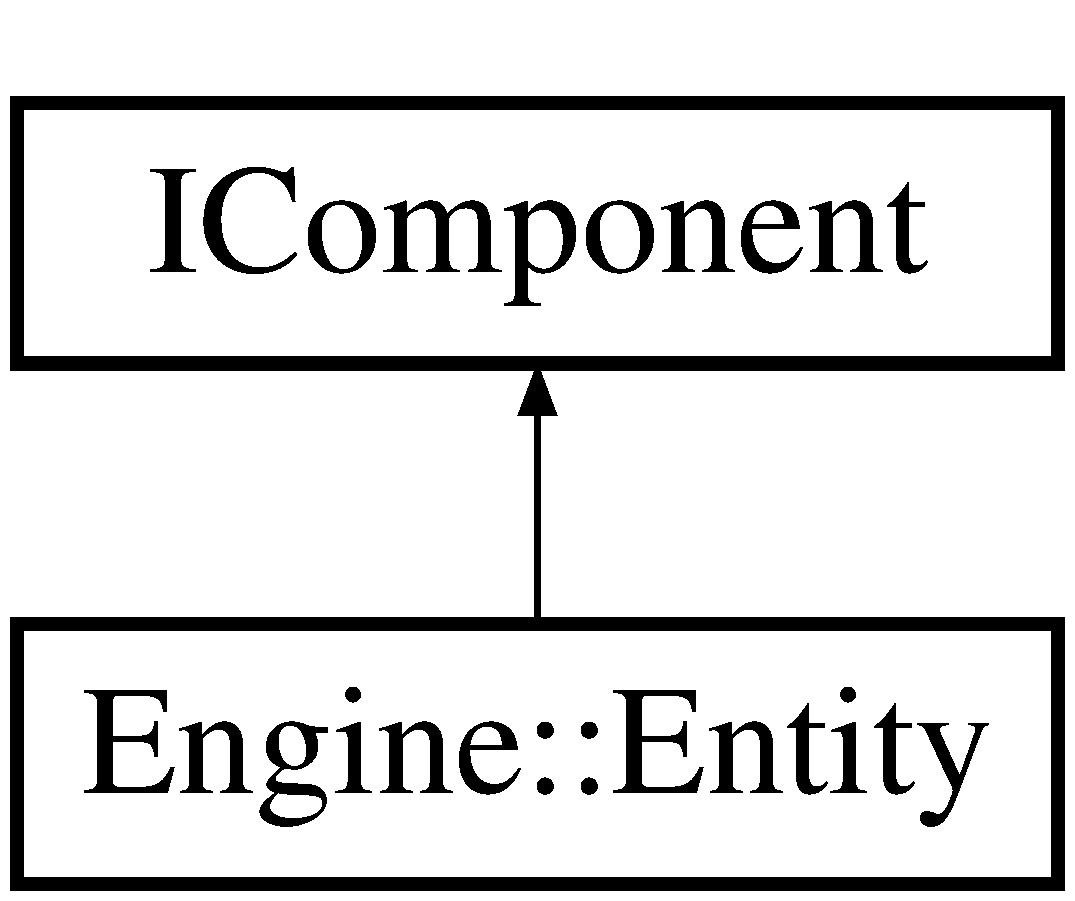
\includegraphics[height=2.000000cm]{classEngine_1_1Entity}
\end{center}
\end{figure}


\subsection{Detailed Description}
The \hyperlink{classEngine_1_1Entity}{Entity} -\/ base component class -\/ for 3\+D Entitys. 

The documentation for this class was generated from the following files\+:\begin{DoxyCompactItemize}
\item 
include/\+Component/entity.\+h\item 
Component/Entity.\+cpp\end{DoxyCompactItemize}

\hypertarget{classEngine_1_1EntityManager}{}\section{Engine\+:\+:Entity\+Manager Class Reference}
\label{classEngine_1_1EntityManager}\index{Engine\+::\+Entity\+Manager@{Engine\+::\+Entity\+Manager}}


The \hyperlink{classEngine_1_1EntityManager}{Entity\+Manager} controlled Entitys ( only 3\+D Entitys )  




{\ttfamily \#include $<$entitymanager.\+h$>$}

Inheritance diagram for Engine\+:\+:Entity\+Manager\+:\begin{figure}[H]
\begin{center}
\leavevmode
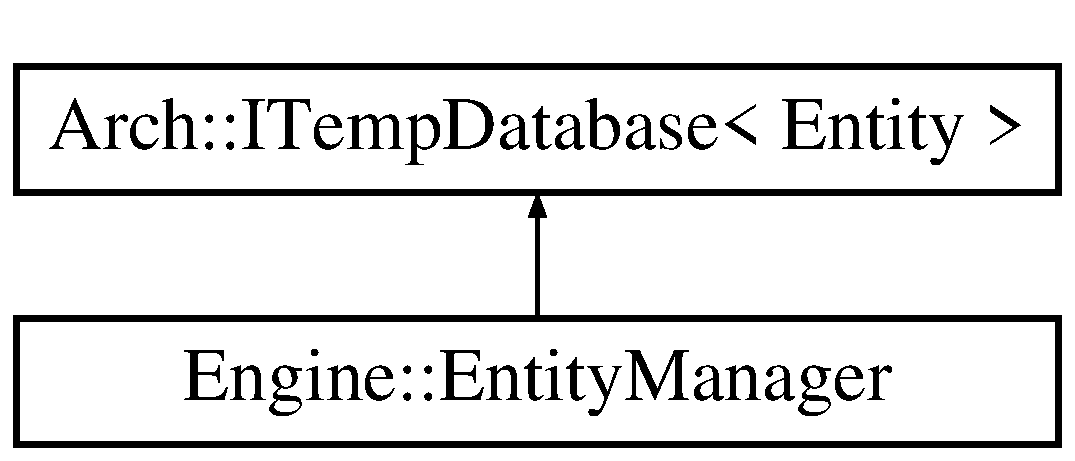
\includegraphics[height=2.000000cm]{classEngine_1_1EntityManager}
\end{center}
\end{figure}
\subsection*{Public Member Functions}
\begin{DoxyCompactItemize}
\item 
\hyperlink{classEngine_1_1Entity}{Entity} $\ast$ \hyperlink{classEngine_1_1EntityManager_aaa426b2acc175d41bb4845e09012c45d}{create\+Entity} (void)
\begin{DoxyCompactList}\small\item\em create\+Entity \end{DoxyCompactList}\item 
\hyperlink{classEngine_1_1Entity}{Entity} $\ast$ \hyperlink{classEngine_1_1EntityManager_a5941c75f3772e78bc2ebb052787b9db4}{get\+Entity} (uint container\+\_\+id)
\begin{DoxyCompactList}\small\item\em get\+Entity \end{DoxyCompactList}\item 
void \hyperlink{classEngine_1_1EntityManager_acc5cdfa18e05d93f0e5c96449383f7fd}{destroy} (uint container\+\_\+id)
\begin{DoxyCompactList}\small\item\em destroy \end{DoxyCompactList}\end{DoxyCompactItemize}


\subsection{Detailed Description}
The \hyperlink{classEngine_1_1EntityManager}{Entity\+Manager} controlled Entitys ( only 3\+D Entitys ) 

Componentv2 Database ( \hyperlink{classEngine_1_1EntityManager}{Entity\+Manager} ) 

\subsection{Member Function Documentation}
\hypertarget{classEngine_1_1EntityManager_aaa426b2acc175d41bb4845e09012c45d}{}\index{Engine\+::\+Entity\+Manager@{Engine\+::\+Entity\+Manager}!create\+Entity@{create\+Entity}}
\index{create\+Entity@{create\+Entity}!Engine\+::\+Entity\+Manager@{Engine\+::\+Entity\+Manager}}
\subsubsection[{create\+Entity(void)}]{\setlength{\rightskip}{0pt plus 5cm}{\bf Entity} $\ast$ Entity\+Manager\+::create\+Entity (
\begin{DoxyParamCaption}
\item[{void}]{}
\end{DoxyParamCaption}
)}\label{classEngine_1_1EntityManager_aaa426b2acc175d41bb4845e09012c45d}


create\+Entity 

\begin{DoxyReturn}{Returns}
\hyperlink{classEngine_1_1Entity}{Entity} Ptr 
\end{DoxyReturn}
\hypertarget{classEngine_1_1EntityManager_acc5cdfa18e05d93f0e5c96449383f7fd}{}\index{Engine\+::\+Entity\+Manager@{Engine\+::\+Entity\+Manager}!destroy@{destroy}}
\index{destroy@{destroy}!Engine\+::\+Entity\+Manager@{Engine\+::\+Entity\+Manager}}
\subsubsection[{destroy(uint container\+\_\+id)}]{\setlength{\rightskip}{0pt plus 5cm}void Entity\+Manager\+::destroy (
\begin{DoxyParamCaption}
\item[{uint}]{container\+\_\+id}
\end{DoxyParamCaption}
)}\label{classEngine_1_1EntityManager_acc5cdfa18e05d93f0e5c96449383f7fd}


destroy 

Destroy a \hyperlink{classEngine_1_1Entity}{Entity} 
\begin{DoxyParams}{Parameters}
{\em container\+\_\+id} & \\
\hline
\end{DoxyParams}
\hypertarget{classEngine_1_1EntityManager_a5941c75f3772e78bc2ebb052787b9db4}{}\index{Engine\+::\+Entity\+Manager@{Engine\+::\+Entity\+Manager}!get\+Entity@{get\+Entity}}
\index{get\+Entity@{get\+Entity}!Engine\+::\+Entity\+Manager@{Engine\+::\+Entity\+Manager}}
\subsubsection[{get\+Entity(uint container\+\_\+id)}]{\setlength{\rightskip}{0pt plus 5cm}{\bf Entity} $\ast$ Entity\+Manager\+::get\+Entity (
\begin{DoxyParamCaption}
\item[{uint}]{container\+\_\+id}
\end{DoxyParamCaption}
)}\label{classEngine_1_1EntityManager_a5941c75f3772e78bc2ebb052787b9db4}


get\+Entity 

Return a \hyperlink{classEngine_1_1Entity}{Entity} Ptr 
\begin{DoxyParams}{Parameters}
{\em container\+\_\+id} & \\
\hline
\end{DoxyParams}
\begin{DoxyReturn}{Returns}
\hyperlink{classEngine_1_1Entity}{Entity} Ptr 
\end{DoxyReturn}


The documentation for this class was generated from the following files\+:\begin{DoxyCompactItemize}
\item 
include/\+Manager/entitymanager.\+h\item 
Engine/\+Manager/Entity\+Manager.\+cpp\end{DoxyCompactItemize}

\hypertarget{structEngine_1_1FontAtlas}{}\section{Engine\+:\+:Font\+Atlas Struct Reference}
\label{structEngine_1_1FontAtlas}\index{Engine\+::\+Font\+Atlas@{Engine\+::\+Font\+Atlas}}
\subsection*{Public Attributes}
\begin{DoxyCompactItemize}
\item 
\hypertarget{structEngine_1_1FontAtlas_a24cccc53bf8444bc8382e6debcc2526c}{}\hyperlink{structEngine_1_1FontAtlasChar}{Font\+Atlas\+Char} {\bfseries chars} \mbox{[}128\mbox{]}\label{structEngine_1_1FontAtlas_a24cccc53bf8444bc8382e6debcc2526c}

\item 
\hypertarget{structEngine_1_1FontAtlas_a3034ba7866ba14966704f9c4d777f9c5}{}int {\bfseries atlas\+\_\+width}\label{structEngine_1_1FontAtlas_a3034ba7866ba14966704f9c4d777f9c5}

\item 
\hypertarget{structEngine_1_1FontAtlas_a29eca98267fd0b2e0acb9e6eff80bae4}{}int {\bfseries atlas\+\_\+height}\label{structEngine_1_1FontAtlas_a29eca98267fd0b2e0acb9e6eff80bae4}

\item 
\hypertarget{structEngine_1_1FontAtlas_af1906195c4a6e0f3d73a2328ac34b6bd}{}\hyperlink{classEngine_1_1Texture}{Texture} $\ast$ {\bfseries texture}\label{structEngine_1_1FontAtlas_af1906195c4a6e0f3d73a2328ac34b6bd}

\end{DoxyCompactItemize}


The documentation for this struct was generated from the following file\+:\begin{DoxyCompactItemize}
\item 
include/\+Manager/fontmanager.\+h\end{DoxyCompactItemize}

\hypertarget{structEngine_1_1FontAtlasChar}{}\section{Engine\+:\+:Font\+Atlas\+Char Struct Reference}
\label{structEngine_1_1FontAtlasChar}\index{Engine\+::\+Font\+Atlas\+Char@{Engine\+::\+Font\+Atlas\+Char}}
\subsection*{Public Attributes}
\begin{DoxyCompactItemize}
\item 
\hypertarget{structEngine_1_1FontAtlasChar_ae21676ec3c222978a599253640a5d95c}{}char {\bfseries c}\label{structEngine_1_1FontAtlasChar_ae21676ec3c222978a599253640a5d95c}

\item 
\hypertarget{structEngine_1_1FontAtlasChar_a7f7ec1fbf9e308f0830d76b582db7c57}{}int {\bfseries x}\label{structEngine_1_1FontAtlasChar_a7f7ec1fbf9e308f0830d76b582db7c57}

\item 
\hypertarget{structEngine_1_1FontAtlasChar_a636dc075713ff5c39d987fdfc797e3ab}{}int {\bfseries y}\label{structEngine_1_1FontAtlasChar_a636dc075713ff5c39d987fdfc797e3ab}

\item 
\hypertarget{structEngine_1_1FontAtlasChar_a63c13ae908a240e99f72c9cb4d290c25}{}int {\bfseries width}\label{structEngine_1_1FontAtlasChar_a63c13ae908a240e99f72c9cb4d290c25}

\item 
\hypertarget{structEngine_1_1FontAtlasChar_a1fe101155e2e13d23e9cf201d45a0f6e}{}int {\bfseries height}\label{structEngine_1_1FontAtlasChar_a1fe101155e2e13d23e9cf201d45a0f6e}

\item 
\hypertarget{structEngine_1_1FontAtlasChar_acaffee47030747472c56c712953becda}{}\hyperlink{structEngine_1_1FontAtlasCharUV}{Font\+Atlas\+Char\+U\+V} {\bfseries uvs} \mbox{[}6\mbox{]}\label{structEngine_1_1FontAtlasChar_acaffee47030747472c56c712953becda}

\end{DoxyCompactItemize}


The documentation for this struct was generated from the following file\+:\begin{DoxyCompactItemize}
\item 
include/\+Manager/fontmanager.\+h\end{DoxyCompactItemize}

\hypertarget{structEngine_1_1FontAtlasCharUV}{}\section{Engine\+:\+:Font\+Atlas\+Char\+U\+V Struct Reference}
\label{structEngine_1_1FontAtlasCharUV}\index{Engine\+::\+Font\+Atlas\+Char\+U\+V@{Engine\+::\+Font\+Atlas\+Char\+U\+V}}
\subsection*{Public Attributes}
\begin{DoxyCompactItemize}
\item 
\hypertarget{structEngine_1_1FontAtlasCharUV_afb2b957046364571bb49636afe953501}{}float {\bfseries u}\label{structEngine_1_1FontAtlasCharUV_afb2b957046364571bb49636afe953501}

\item 
\hypertarget{structEngine_1_1FontAtlasCharUV_a7eee14e444af1f7fc0f49008347f764d}{}float {\bfseries v}\label{structEngine_1_1FontAtlasCharUV_a7eee14e444af1f7fc0f49008347f764d}

\end{DoxyCompactItemize}


The documentation for this struct was generated from the following file\+:\begin{DoxyCompactItemize}
\item 
include/\+Manager/fontmanager.\+h\end{DoxyCompactItemize}

\hypertarget{classEngine_1_1FontManager}{}\section{Engine\+:\+:Font\+Manager Class Reference}
\label{classEngine_1_1FontManager}\index{Engine\+::\+Font\+Manager@{Engine\+::\+Font\+Manager}}


The \hyperlink{classEngine_1_1FontManager}{Font\+Manager} managed the Fonts.  




{\ttfamily \#include $<$fontmanager.\+h$>$}

\subsection*{Public Types}
\begin{DoxyCompactItemize}
\item 
using \hyperlink{classEngine_1_1FontManager_aba32832f74f13b0bec53d5132f78bcc3}{Char\+Mapping} = std\+::map$<$ char, \hyperlink{classEngine_1_1Texture}{Texture} $\ast$ $>$
\end{DoxyCompactItemize}
\subsection*{Public Member Functions}
\begin{DoxyCompactItemize}
\item 
\hypertarget{classEngine_1_1FontManager_aef1290f13e68f6c22fe5a9341bf04de9}{}void {\bfseries finish} (void)\label{classEngine_1_1FontManager_aef1290f13e68f6c22fe5a9341bf04de9}

\item 
\hypertarget{classEngine_1_1FontManager_ab6edb246a77230f5ef25ea065ce9bd8f}{}\hyperlink{structEngine_1_1FontAtlas}{Font\+Atlas} {\bfseries create\+Font\+Atlas} (const std\+::string \&ttf\+\_\+file)\label{classEngine_1_1FontManager_ab6edb246a77230f5ef25ea065ce9bd8f}

\item 
F\+T\+\_\+\+Face \hyperlink{classEngine_1_1FontManager_a6e6afb29d8dde70cfd44a9a062a70e5b}{create\+Font\+Face} (const std\+::string \&ttf\+\_\+file)
\begin{DoxyCompactList}\small\item\em create\+Font\+Face \end{DoxyCompactList}\item 
void \hyperlink{classEngine_1_1FontManager_a25e57a935eaa136bdca2aa477d6f0bbf}{load} (F\+T\+\_\+\+Face face, const std\+::string \&asci)
\begin{DoxyCompactList}\small\item\em load \end{DoxyCompactList}\item 
\hypertarget{classEngine_1_1FontManager_abef4ff92e3d53fc92785680af0e017b4}{}void {\bfseries unload} (void)\label{classEngine_1_1FontManager_abef4ff92e3d53fc92785680af0e017b4}

\item 
\hyperlink{classEngine_1_1Texture}{Texture} $\ast$ \hyperlink{classEngine_1_1FontManager_a4ae277341d1f3b33dfab74ab2f175587}{get\+Char\+Texture} (char c)  throw ( std\+::runtime\+\_\+error )
\begin{DoxyCompactList}\small\item\em get\+Char\+Texture \end{DoxyCompactList}\item 
void \hyperlink{classEngine_1_1FontManager_aa036cdf0c0646b46069eb18732d81f00}{Char\+Register} (char c, \hyperlink{classEngine_1_1Texture}{Texture} $\ast$buffer)
\begin{DoxyCompactList}\small\item\em Char\+Register. \end{DoxyCompactList}\end{DoxyCompactItemize}
\subsection*{Static Public Member Functions}
\begin{DoxyCompactItemize}
\item 
static \hyperlink{classEngine_1_1FontManager}{Font\+Manager} $\ast$ \hyperlink{classEngine_1_1FontManager_a5af489a1003b2d1db331ae72e560de3f}{get\+Singleton\+Ptr} (void)
\begin{DoxyCompactList}\small\item\em get\+Singleton\+Ptr \end{DoxyCompactList}\end{DoxyCompactItemize}
\subsection*{Protected Member Functions}
\begin{DoxyCompactItemize}
\item 
\hypertarget{classEngine_1_1FontManager_a051c7bda65ef456de8638acc30073c41}{}\hyperlink{classVector2}{Vector2f} {\bfseries get\+Atlas\+Vector} (F\+T\+\_\+\+Face font)\label{classEngine_1_1FontManager_a051c7bda65ef456de8638acc30073c41}

\end{DoxyCompactItemize}


\subsection{Detailed Description}
The \hyperlink{classEngine_1_1FontManager}{Font\+Manager} managed the Fonts. 

Managemant of Fonts


\begin{DoxyItemize}
\item using Free\+Type library
\item Create char Textures 
\end{DoxyItemize}

\subsection{Member Typedef Documentation}
\hypertarget{classEngine_1_1FontManager_aba32832f74f13b0bec53d5132f78bcc3}{}\index{Engine\+::\+Font\+Manager@{Engine\+::\+Font\+Manager}!Char\+Mapping@{Char\+Mapping}}
\index{Char\+Mapping@{Char\+Mapping}!Engine\+::\+Font\+Manager@{Engine\+::\+Font\+Manager}}
\subsubsection[{Char\+Mapping}]{\setlength{\rightskip}{0pt plus 5cm}using {\bf Engine\+::\+Font\+Manager\+::\+Char\+Mapping} =  std\+::map$<$ char , {\bf Texture} $\ast$ $>$}\label{classEngine_1_1FontManager_aba32832f74f13b0bec53d5132f78bcc3}
Save Char Textures 

\subsection{Member Function Documentation}
\hypertarget{classEngine_1_1FontManager_aa036cdf0c0646b46069eb18732d81f00}{}\index{Engine\+::\+Font\+Manager@{Engine\+::\+Font\+Manager}!Char\+Register@{Char\+Register}}
\index{Char\+Register@{Char\+Register}!Engine\+::\+Font\+Manager@{Engine\+::\+Font\+Manager}}
\subsubsection[{Char\+Register(char c, Texture $\ast$buffer)}]{\setlength{\rightskip}{0pt plus 5cm}void Font\+Manager\+::\+Char\+Register (
\begin{DoxyParamCaption}
\item[{char}]{c, }
\item[{{\bf Texture} $\ast$}]{buffer}
\end{DoxyParamCaption}
)}\label{classEngine_1_1FontManager_aa036cdf0c0646b46069eb18732d81f00}


Char\+Register. 

Save a char with Pixeldata ( aka. \hyperlink{classEngine_1_1Texture}{Texture} ) 
\begin{DoxyParams}{Parameters}
{\em c} & \\
\hline
{\em buffer} & \\
\hline
\end{DoxyParams}
\hypertarget{classEngine_1_1FontManager_a6e6afb29d8dde70cfd44a9a062a70e5b}{}\index{Engine\+::\+Font\+Manager@{Engine\+::\+Font\+Manager}!create\+Font\+Face@{create\+Font\+Face}}
\index{create\+Font\+Face@{create\+Font\+Face}!Engine\+::\+Font\+Manager@{Engine\+::\+Font\+Manager}}
\subsubsection[{create\+Font\+Face(const std\+::string \&ttf\+\_\+file)}]{\setlength{\rightskip}{0pt plus 5cm}F\+T\+\_\+\+Face Font\+Manager\+::create\+Font\+Face (
\begin{DoxyParamCaption}
\item[{const std\+::string \&}]{ttf\+\_\+file}
\end{DoxyParamCaption}
)}\label{classEngine_1_1FontManager_a6e6afb29d8dde70cfd44a9a062a70e5b}


create\+Font\+Face 

Create Font from .ttf file 
\begin{DoxyParams}{Parameters}
{\em ttf\+\_\+file} & \\
\hline
\end{DoxyParams}
\begin{DoxyReturn}{Returns}

\end{DoxyReturn}
\hypertarget{classEngine_1_1FontManager_a4ae277341d1f3b33dfab74ab2f175587}{}\index{Engine\+::\+Font\+Manager@{Engine\+::\+Font\+Manager}!get\+Char\+Texture@{get\+Char\+Texture}}
\index{get\+Char\+Texture@{get\+Char\+Texture}!Engine\+::\+Font\+Manager@{Engine\+::\+Font\+Manager}}
\subsubsection[{get\+Char\+Texture(char c)}]{\setlength{\rightskip}{0pt plus 5cm}{\bf Texture} $\ast$ Font\+Manager\+::get\+Char\+Texture (
\begin{DoxyParamCaption}
\item[{char}]{c}
\end{DoxyParamCaption}
) throw  std\+::runtime\+\_\+error) }\label{classEngine_1_1FontManager_a4ae277341d1f3b33dfab74ab2f175587}


get\+Char\+Texture 

Return \hyperlink{classEngine_1_1Texture}{Texture} by char 
\begin{DoxyParams}{Parameters}
{\em c} & \\
\hline
\end{DoxyParams}
\begin{DoxyReturn}{Returns}

\end{DoxyReturn}
\hypertarget{classEngine_1_1FontManager_a5af489a1003b2d1db331ae72e560de3f}{}\index{Engine\+::\+Font\+Manager@{Engine\+::\+Font\+Manager}!get\+Singleton\+Ptr@{get\+Singleton\+Ptr}}
\index{get\+Singleton\+Ptr@{get\+Singleton\+Ptr}!Engine\+::\+Font\+Manager@{Engine\+::\+Font\+Manager}}
\subsubsection[{get\+Singleton\+Ptr(void)}]{\setlength{\rightskip}{0pt plus 5cm}{\bf Font\+Manager} $\ast$ Font\+Manager\+::get\+Singleton\+Ptr (
\begin{DoxyParamCaption}
\item[{void}]{}
\end{DoxyParamCaption}
)\hspace{0.3cm}{\ttfamily [static]}}\label{classEngine_1_1FontManager_a5af489a1003b2d1db331ae72e560de3f}


get\+Singleton\+Ptr 

Return \hyperlink{classEngine_1_1FontManager}{Font\+Manager} Instance \begin{DoxyReturn}{Returns}

\end{DoxyReturn}
\hypertarget{classEngine_1_1FontManager_a25e57a935eaa136bdca2aa477d6f0bbf}{}\index{Engine\+::\+Font\+Manager@{Engine\+::\+Font\+Manager}!load@{load}}
\index{load@{load}!Engine\+::\+Font\+Manager@{Engine\+::\+Font\+Manager}}
\subsubsection[{load(\+F\+T\+\_\+\+Face face, const std\+::string \&asci)}]{\setlength{\rightskip}{0pt plus 5cm}void Font\+Manager\+::load (
\begin{DoxyParamCaption}
\item[{F\+T\+\_\+\+Face}]{face, }
\item[{const std\+::string \&}]{asci}
\end{DoxyParamCaption}
)}\label{classEngine_1_1FontManager_a25e57a935eaa136bdca2aa477d6f0bbf}


load 

Load Font\+Face and create Char Textures


\begin{DoxyParams}{Parameters}
{\em face} & \\
\hline
{\em asci} & \+: !\#\$\%\&\textquotesingle{}()$\ast$+,-\/./0123456789\+:;$<$=$>$?\mbox{[}\textbackslash{}\mbox{]}$^\wedge$\+\_\+`abcdefghijklmnopqrstuvwxyz\{$\vert$\}$\sim$ \\
\hline
\end{DoxyParams}


The documentation for this class was generated from the following files\+:\begin{DoxyCompactItemize}
\item 
include/\+Manager/fontmanager.\+h\item 
Engine/\+Manager/Font\+Manager.\+cpp\end{DoxyCompactItemize}

\hypertarget{classEngine_1_1FrameBuffer}{}\section{Engine\+:\+:Frame\+Buffer Class Reference}
\label{classEngine_1_1FrameBuffer}\index{Engine\+::\+Frame\+Buffer@{Engine\+::\+Frame\+Buffer}}


The \hyperlink{classEngine_1_1FrameBuffer}{Frame\+Buffer} class.  




{\ttfamily \#include $<$framebuffer.\+h$>$}

\subsection*{Public Types}
\begin{DoxyCompactItemize}
\item 
\hypertarget{classEngine_1_1FrameBuffer_aeb2fbf0213916abf0afbfb31921e7632}{}enum \{ \\*
{\bfseries F\+B\+\_\+\+T\+E\+X\+T\+U\+R\+E\+\_\+\+A\+R\+R\+A\+Y0}, 
{\bfseries F\+B\+\_\+\+T\+E\+X\+T\+U\+R\+E\+\_\+\+A\+R\+R\+A\+Y1}, 
{\bfseries F\+B\+\_\+\+T\+E\+X\+T\+U\+R\+E\+\_\+\+A\+R\+R\+A\+Y2}, 
{\bfseries F\+B\+\_\+\+T\+E\+X\+T\+U\+R\+E\+\_\+\+A\+R\+R\+A\+Y3}, 
\\*
{\bfseries F\+B\+\_\+\+T\+E\+X\+T\+U\+R\+E\+\_\+\+A\+R\+R\+A\+Y4}, 
{\bfseries F\+B\+\_\+\+T\+E\+X\+T\+U\+R\+E\+\_\+\+A\+R\+R\+A\+Y5}, 
{\bfseries F\+B\+\_\+\+T\+E\+X\+T\+U\+R\+E\+\_\+\+A\+R\+R\+A\+Y6}, 
{\bfseries F\+B\+\_\+\+T\+E\+X\+T\+U\+R\+E\+\_\+\+A\+R\+R\+A\+Y7}, 
\\*
{\bfseries F\+B\+\_\+\+T\+E\+X\+T\+U\+R\+E\+\_\+\+A\+R\+R\+A\+Y8}, 
{\bfseries F\+B\+\_\+\+T\+E\+X\+T\+U\+R\+E\+\_\+\+A\+R\+R\+A\+Y9}, 
{\bfseries F\+B\+\_\+\+T\+E\+X\+T\+U\+R\+E\+\_\+\+A\+R\+R\+A\+Y10}, 
{\bfseries F\+B\+\_\+\+T\+E\+X\+T\+U\+R\+E\+\_\+\+A\+R\+R\+A\+Y11}, 
\\*
{\bfseries F\+B\+\_\+\+T\+E\+X\+T\+U\+R\+E\+\_\+\+A\+R\+R\+A\+Y12}, 
{\bfseries F\+B\+\_\+\+T\+E\+X\+T\+U\+R\+E\+\_\+\+A\+R\+R\+A\+Y13}, 
{\bfseries F\+B\+\_\+\+T\+E\+X\+T\+U\+R\+E\+\_\+\+A\+R\+R\+A\+Y14}, 
{\bfseries F\+B\+\_\+\+T\+E\+X\+T\+U\+R\+E\+\_\+\+A\+R\+R\+A\+Y15}
 \}\label{classEngine_1_1FrameBuffer_aeb2fbf0213916abf0afbfb31921e7632}

\end{DoxyCompactItemize}
\subsection*{Public Member Functions}
\begin{DoxyCompactItemize}
\item 
\hypertarget{classEngine_1_1FrameBuffer_aab4c897d360f51c5a96b4782e67e98a9}{}{\bfseries Frame\+Buffer} (int width, int height)\label{classEngine_1_1FrameBuffer_aab4c897d360f51c5a96b4782e67e98a9}

\item 
void \hyperlink{classEngine_1_1FrameBuffer_aa81f1fe9336c5afb85da9204cd288f8b}{Read\+Frame\+Buffer} (void)
\begin{DoxyCompactList}\small\item\em Read\+Frame\+Buffer. \end{DoxyCompactList}\item 
void \hyperlink{classEngine_1_1FrameBuffer_a9a01e5e19f7a529a7e9e88938c8c62e7}{Draw\+Frame\+Buffer} (void)
\begin{DoxyCompactList}\small\item\em Draw\+Frame\+Buffer. \end{DoxyCompactList}\item 
void \hyperlink{classEngine_1_1FrameBuffer_a94eac6daf7539617d189c302243712b1}{Bind\+Frame\+Buffer} (void)
\begin{DoxyCompactList}\small\item\em Bind\+Frame\+Buffer. \end{DoxyCompactList}\item 
\hypertarget{classEngine_1_1FrameBuffer_ae0194d4d72f2f89c66178b85c1076941}{}void \hyperlink{classEngine_1_1FrameBuffer_ae0194d4d72f2f89c66178b85c1076941}{Unbind} ()\label{classEngine_1_1FrameBuffer_ae0194d4d72f2f89c66178b85c1076941}

\begin{DoxyCompactList}\small\item\em Unbind. \end{DoxyCompactList}\item 
void \hyperlink{classEngine_1_1FrameBuffer_aaca72b1f1e7a4d71df1431cf7409b014}{Bind\+Texture\+Array} (\hyperlink{classEngine_1_1Texture}{Texture} $\ast$texture, G\+Lenum attachment)
\begin{DoxyCompactList}\small\item\em \hyperlink{classEngine_1_1FrameBuffer_aaca72b1f1e7a4d71df1431cf7409b014}{Frame\+Buffer\+::\+Bind\+Texture\+Array}. \end{DoxyCompactList}\item 
\hypertarget{classEngine_1_1FrameBuffer_aed40625d398bea209d8fc9e864ac0a3e}{}void {\bfseries Add\+Texture} (\hyperlink{classEngine_1_1Texture}{Texture} $\ast$texture, G\+Lenum attachment)\label{classEngine_1_1FrameBuffer_aed40625d398bea209d8fc9e864ac0a3e}

\item 
void \hyperlink{classEngine_1_1FrameBuffer_a636279ddc844348854635f660840fba1}{Bind\+Texture\+Layer} (\hyperlink{classEngine_1_1Texture}{Texture} $\ast$texture, int layer, G\+Lenum attachment)
\begin{DoxyCompactList}\small\item\em \hyperlink{classEngine_1_1FrameBuffer_a636279ddc844348854635f660840fba1}{Frame\+Buffer\+::\+Bind\+Texture\+Layer}. \end{DoxyCompactList}\item 
void \hyperlink{classEngine_1_1FrameBuffer_a29c67a4d8a1f3037e94d9c0664eef744}{Bind\+Texture} (\hyperlink{classEngine_1_1Texture}{Texture} $\ast$texture, G\+Lenum attachment)
\begin{DoxyCompactList}\small\item\em \hyperlink{classEngine_1_1FrameBuffer_a29c67a4d8a1f3037e94d9c0664eef744}{Frame\+Buffer\+::\+Bind\+Texture}. \end{DoxyCompactList}\item 
void \hyperlink{classEngine_1_1FrameBuffer_afe51f4e52ebb753c7bbd3f780d92f3d8}{Bind\+Render\+Buffer} (\hyperlink{classEngine_1_1Texture}{Texture} $\ast$texture, G\+Lenum attachment)
\begin{DoxyCompactList}\small\item\em \hyperlink{classEngine_1_1FrameBuffer_afe51f4e52ebb753c7bbd3f780d92f3d8}{Frame\+Buffer\+::\+Bind\+Render\+Buffer}. \end{DoxyCompactList}\item 
\hyperlink{classEngine_1_1Texture}{Texture} $\ast$ \hyperlink{classEngine_1_1FrameBuffer_ab34cd5630598712e9961caa47aba6fcf}{get\+Render\+Buffer} (G\+Lenum attachment)
\begin{DoxyCompactList}\small\item\em get\+Render\+Buffer \end{DoxyCompactList}\item 
\hyperlink{classEngine_1_1Texture}{Texture} $\ast$ \hyperlink{classEngine_1_1FrameBuffer_a991caed6a2eb5bc2f21a37e741dc261b}{get\+Texture} (G\+Lenum attachment)
\begin{DoxyCompactList}\small\item\em get\+Texture \end{DoxyCompactList}\item 
int \hyperlink{classEngine_1_1FrameBuffer_a2f9f76269e95a76a889b7ea468e5fc7f}{get\+Frame\+Width} (void)
\begin{DoxyCompactList}\small\item\em get\+Frame\+Width \end{DoxyCompactList}\item 
int \hyperlink{classEngine_1_1FrameBuffer_a77a9253035765ef36d0def08a68068d4}{get\+Frame\+Height} (void)
\begin{DoxyCompactList}\small\item\em get\+Frame\+Height \end{DoxyCompactList}\end{DoxyCompactItemize}


\subsection{Detailed Description}
The \hyperlink{classEngine_1_1FrameBuffer}{Frame\+Buffer} class. 

\subsection{Member Function Documentation}
\hypertarget{classEngine_1_1FrameBuffer_a94eac6daf7539617d189c302243712b1}{}\index{Engine\+::\+Frame\+Buffer@{Engine\+::\+Frame\+Buffer}!Bind\+Frame\+Buffer@{Bind\+Frame\+Buffer}}
\index{Bind\+Frame\+Buffer@{Bind\+Frame\+Buffer}!Engine\+::\+Frame\+Buffer@{Engine\+::\+Frame\+Buffer}}
\subsubsection[{Bind\+Frame\+Buffer(void)}]{\setlength{\rightskip}{0pt plus 5cm}void Frame\+Buffer\+::\+Bind\+Frame\+Buffer (
\begin{DoxyParamCaption}
\item[{void}]{}
\end{DoxyParamCaption}
)}\label{classEngine_1_1FrameBuffer_a94eac6daf7539617d189c302243712b1}


Bind\+Frame\+Buffer. 

Bind Framebuffer -\/ render to texture \hypertarget{classEngine_1_1FrameBuffer_afe51f4e52ebb753c7bbd3f780d92f3d8}{}\index{Engine\+::\+Frame\+Buffer@{Engine\+::\+Frame\+Buffer}!Bind\+Render\+Buffer@{Bind\+Render\+Buffer}}
\index{Bind\+Render\+Buffer@{Bind\+Render\+Buffer}!Engine\+::\+Frame\+Buffer@{Engine\+::\+Frame\+Buffer}}
\subsubsection[{Bind\+Render\+Buffer(\+Texture $\ast$texture, G\+Lenum attachment)}]{\setlength{\rightskip}{0pt plus 5cm}void Frame\+Buffer\+::\+Bind\+Render\+Buffer (
\begin{DoxyParamCaption}
\item[{{\bf Texture} $\ast$}]{texture, }
\item[{G\+Lenum}]{attachment}
\end{DoxyParamCaption}
)}\label{classEngine_1_1FrameBuffer_afe51f4e52ebb753c7bbd3f780d92f3d8}


\hyperlink{classEngine_1_1FrameBuffer_afe51f4e52ebb753c7bbd3f780d92f3d8}{Frame\+Buffer\+::\+Bind\+Render\+Buffer}. 

Attachments\+:

-\/$>$ diffuse \+: G\+L\+\_\+\+C\+O\+L\+O\+R\+\_\+\+A\+T\+T\+A\+C\+H\+M\+E\+N\+T0 -\/$>$ position \+: G\+L\+\_\+\+C\+O\+L\+O\+R\+\_\+\+A\+T\+T\+A\+C\+H\+M\+E\+N\+T1 -\/$>$ normals \+: G\+L\+\_\+\+C\+O\+L\+O\+R\+\_\+\+A\+T\+T\+A\+C\+H\+M\+E\+N\+T2 -\/$>$ depth \+: G\+L\+\_\+\+D\+E\+P\+T\+H\+\_\+\+A\+T\+T\+A\+C\+H\+M\+E\+N\+T


\begin{DoxyParams}{Parameters}
{\em texture} & \\
\hline
{\em attachment} & -\/$>$ diffuse \+: G\+L\+\_\+\+C\+O\+L\+O\+R\+\_\+\+A\+T\+T\+A\+C\+H\+M\+E\+N\+T0 -\/$>$ position \+: G\+L\+\_\+\+C\+O\+L\+O\+R\+\_\+\+A\+T\+T\+A\+C\+H\+M\+E\+N\+T1 -\/$>$ normals \+: G\+L\+\_\+\+C\+O\+L\+O\+R\+\_\+\+A\+T\+T\+A\+C\+H\+M\+E\+N\+T2 -\/$>$ depth \+: G\+L\+\_\+\+D\+E\+P\+T\+H\+\_\+\+A\+T\+T\+A\+C\+H\+M\+E\+N\+T\\
\hline
{\em texture} & \\
\hline
{\em attachment} & \\
\hline
\end{DoxyParams}
\hypertarget{classEngine_1_1FrameBuffer_a29c67a4d8a1f3037e94d9c0664eef744}{}\index{Engine\+::\+Frame\+Buffer@{Engine\+::\+Frame\+Buffer}!Bind\+Texture@{Bind\+Texture}}
\index{Bind\+Texture@{Bind\+Texture}!Engine\+::\+Frame\+Buffer@{Engine\+::\+Frame\+Buffer}}
\subsubsection[{Bind\+Texture(\+Texture $\ast$texture, G\+Lenum attachment)}]{\setlength{\rightskip}{0pt plus 5cm}void Frame\+Buffer\+::\+Bind\+Texture (
\begin{DoxyParamCaption}
\item[{{\bf Texture} $\ast$}]{texture, }
\item[{G\+Lenum}]{attachment}
\end{DoxyParamCaption}
)}\label{classEngine_1_1FrameBuffer_a29c67a4d8a1f3037e94d9c0664eef744}


\hyperlink{classEngine_1_1FrameBuffer_a29c67a4d8a1f3037e94d9c0664eef744}{Frame\+Buffer\+::\+Bind\+Texture}. 

Attachments\+:

-\/$>$ diffuse \+: G\+L\+\_\+\+C\+O\+L\+O\+R\+\_\+\+A\+T\+T\+A\+C\+H\+M\+E\+N\+T0 -\/$>$ position \+: G\+L\+\_\+\+C\+O\+L\+O\+R\+\_\+\+A\+T\+T\+A\+C\+H\+M\+E\+N\+T1 -\/$>$ normals \+: G\+L\+\_\+\+C\+O\+L\+O\+R\+\_\+\+A\+T\+T\+A\+C\+H\+M\+E\+N\+T2


\begin{DoxyParams}{Parameters}
{\em texture} & \\
\hline
{\em attachment} & -\/$>$ diffuse \+: G\+L\+\_\+\+C\+O\+L\+O\+R\+\_\+\+A\+T\+T\+A\+C\+H\+M\+E\+N\+T0 -\/$>$ position \+: G\+L\+\_\+\+C\+O\+L\+O\+R\+\_\+\+A\+T\+T\+A\+C\+H\+M\+E\+N\+T1 -\/$>$ normals \+: G\+L\+\_\+\+C\+O\+L\+O\+R\+\_\+\+A\+T\+T\+A\+C\+H\+M\+E\+N\+T2 -\/$>$ depth \+: G\+L\+\_\+\+D\+E\+P\+T\+H\+\_\+\+A\+T\+T\+A\+C\+H\+M\+E\+N\+T\\
\hline
{\em texture} & \\
\hline
{\em attachment} & \\
\hline
\end{DoxyParams}
\hypertarget{classEngine_1_1FrameBuffer_aaca72b1f1e7a4d71df1431cf7409b014}{}\index{Engine\+::\+Frame\+Buffer@{Engine\+::\+Frame\+Buffer}!Bind\+Texture\+Array@{Bind\+Texture\+Array}}
\index{Bind\+Texture\+Array@{Bind\+Texture\+Array}!Engine\+::\+Frame\+Buffer@{Engine\+::\+Frame\+Buffer}}
\subsubsection[{Bind\+Texture\+Array(\+Texture $\ast$texture, G\+Lenum attachment)}]{\setlength{\rightskip}{0pt plus 5cm}void Frame\+Buffer\+::\+Bind\+Texture\+Array (
\begin{DoxyParamCaption}
\item[{{\bf Texture} $\ast$}]{texture, }
\item[{G\+Lenum}]{attachment}
\end{DoxyParamCaption}
)}\label{classEngine_1_1FrameBuffer_aaca72b1f1e7a4d71df1431cf7409b014}


\hyperlink{classEngine_1_1FrameBuffer_aaca72b1f1e7a4d71df1431cf7409b014}{Frame\+Buffer\+::\+Bind\+Texture\+Array}. 

\hyperlink{classEngine_1_1Texture}{Texture} \+: \hyperlink{classEngine_1_1Texture}{Texture} Array Attachments \+: F\+B\+\_\+\+T\+E\+X\+T\+U\+R\+E\+\_\+\+A\+R\+R\+A\+Y0 + i


\begin{DoxyParams}{Parameters}
{\em texture} & \\
\hline
{\em attachment} & \\
\hline
\end{DoxyParams}
\hypertarget{classEngine_1_1FrameBuffer_a636279ddc844348854635f660840fba1}{}\index{Engine\+::\+Frame\+Buffer@{Engine\+::\+Frame\+Buffer}!Bind\+Texture\+Layer@{Bind\+Texture\+Layer}}
\index{Bind\+Texture\+Layer@{Bind\+Texture\+Layer}!Engine\+::\+Frame\+Buffer@{Engine\+::\+Frame\+Buffer}}
\subsubsection[{Bind\+Texture\+Layer(\+Texture $\ast$texture, int layer, G\+Lenum attachment)}]{\setlength{\rightskip}{0pt plus 5cm}void Frame\+Buffer\+::\+Bind\+Texture\+Layer (
\begin{DoxyParamCaption}
\item[{{\bf Texture} $\ast$}]{texture, }
\item[{int}]{layer, }
\item[{G\+Lenum}]{attachment}
\end{DoxyParamCaption}
)}\label{classEngine_1_1FrameBuffer_a636279ddc844348854635f660840fba1}


\hyperlink{classEngine_1_1FrameBuffer_a636279ddc844348854635f660840fba1}{Frame\+Buffer\+::\+Bind\+Texture\+Layer}. 

\hyperlink{classEngine_1_1Texture}{Texture} \+: \hyperlink{classEngine_1_1Texture}{Texture} Array Attachments \+: G\+L\+\_\+\+C\+O\+L\+O\+R\+\_\+\+A\+T\+T\+A\+C\+H\+M\+E\+N\+T0 + i Layer \+: \hyperlink{classEngine_1_1Texture}{Texture} \hyperlink{classEngine_1_1Position}{Position} from Array


\begin{DoxyParams}{Parameters}
{\em texture} & \\
\hline
{\em attachment} & \\
\hline
{\em layer} & \hyperlink{classEngine_1_1Texture}{Texture} \+: \hyperlink{classEngine_1_1Texture}{Texture} Array Attachments\+: G\+L\+\_\+\+C\+O\+L\+O\+R\+\_\+\+A\+T\+T\+A\+C\+H\+M\+E\+N\+T0 + i Layer \+: \hyperlink{classEngine_1_1Texture}{Texture} \hyperlink{classEngine_1_1Position}{Position} from Array\\
\hline
{\em texture} & \\
\hline
{\em attachment} & \\
\hline
{\em layer} & \\
\hline
\end{DoxyParams}
\hypertarget{classEngine_1_1FrameBuffer_a9a01e5e19f7a529a7e9e88938c8c62e7}{}\index{Engine\+::\+Frame\+Buffer@{Engine\+::\+Frame\+Buffer}!Draw\+Frame\+Buffer@{Draw\+Frame\+Buffer}}
\index{Draw\+Frame\+Buffer@{Draw\+Frame\+Buffer}!Engine\+::\+Frame\+Buffer@{Engine\+::\+Frame\+Buffer}}
\subsubsection[{Draw\+Frame\+Buffer(void)}]{\setlength{\rightskip}{0pt plus 5cm}void Frame\+Buffer\+::\+Draw\+Frame\+Buffer (
\begin{DoxyParamCaption}
\item[{void}]{}
\end{DoxyParamCaption}
)}\label{classEngine_1_1FrameBuffer_a9a01e5e19f7a529a7e9e88938c8c62e7}


Draw\+Frame\+Buffer. 

Enable Draw Mode \hypertarget{classEngine_1_1FrameBuffer_a77a9253035765ef36d0def08a68068d4}{}\index{Engine\+::\+Frame\+Buffer@{Engine\+::\+Frame\+Buffer}!get\+Frame\+Height@{get\+Frame\+Height}}
\index{get\+Frame\+Height@{get\+Frame\+Height}!Engine\+::\+Frame\+Buffer@{Engine\+::\+Frame\+Buffer}}
\subsubsection[{get\+Frame\+Height(void)}]{\setlength{\rightskip}{0pt plus 5cm}int Frame\+Buffer\+::get\+Frame\+Height (
\begin{DoxyParamCaption}
\item[{void}]{}
\end{DoxyParamCaption}
)}\label{classEngine_1_1FrameBuffer_a77a9253035765ef36d0def08a68068d4}


get\+Frame\+Height 

Return Frame height size \begin{DoxyReturn}{Returns}

\end{DoxyReturn}
\hypertarget{classEngine_1_1FrameBuffer_a2f9f76269e95a76a889b7ea468e5fc7f}{}\index{Engine\+::\+Frame\+Buffer@{Engine\+::\+Frame\+Buffer}!get\+Frame\+Width@{get\+Frame\+Width}}
\index{get\+Frame\+Width@{get\+Frame\+Width}!Engine\+::\+Frame\+Buffer@{Engine\+::\+Frame\+Buffer}}
\subsubsection[{get\+Frame\+Width(void)}]{\setlength{\rightskip}{0pt plus 5cm}int Frame\+Buffer\+::get\+Frame\+Width (
\begin{DoxyParamCaption}
\item[{void}]{}
\end{DoxyParamCaption}
)}\label{classEngine_1_1FrameBuffer_a2f9f76269e95a76a889b7ea468e5fc7f}


get\+Frame\+Width 

Return Frame width size \begin{DoxyReturn}{Returns}

\end{DoxyReturn}
\hypertarget{classEngine_1_1FrameBuffer_ab34cd5630598712e9961caa47aba6fcf}{}\index{Engine\+::\+Frame\+Buffer@{Engine\+::\+Frame\+Buffer}!get\+Render\+Buffer@{get\+Render\+Buffer}}
\index{get\+Render\+Buffer@{get\+Render\+Buffer}!Engine\+::\+Frame\+Buffer@{Engine\+::\+Frame\+Buffer}}
\subsubsection[{get\+Render\+Buffer(\+G\+Lenum attachment)}]{\setlength{\rightskip}{0pt plus 5cm}{\bf Texture} $\ast$ Frame\+Buffer\+::get\+Render\+Buffer (
\begin{DoxyParamCaption}
\item[{G\+Lenum}]{attachment}
\end{DoxyParamCaption}
)}\label{classEngine_1_1FrameBuffer_ab34cd5630598712e9961caa47aba6fcf}


get\+Render\+Buffer 

Return Render\+Buffer when is Binded 
\begin{DoxyParams}{Parameters}
{\em attachment} & \\
\hline
\end{DoxyParams}
\begin{DoxyReturn}{Returns}

\end{DoxyReturn}
\hypertarget{classEngine_1_1FrameBuffer_a991caed6a2eb5bc2f21a37e741dc261b}{}\index{Engine\+::\+Frame\+Buffer@{Engine\+::\+Frame\+Buffer}!get\+Texture@{get\+Texture}}
\index{get\+Texture@{get\+Texture}!Engine\+::\+Frame\+Buffer@{Engine\+::\+Frame\+Buffer}}
\subsubsection[{get\+Texture(\+G\+Lenum attachment)}]{\setlength{\rightskip}{0pt plus 5cm}{\bf Texture} $\ast$ Frame\+Buffer\+::get\+Texture (
\begin{DoxyParamCaption}
\item[{G\+Lenum}]{attachment}
\end{DoxyParamCaption}
)}\label{classEngine_1_1FrameBuffer_a991caed6a2eb5bc2f21a37e741dc261b}


get\+Texture 

Return \hyperlink{classEngine_1_1Texture}{Texture} wen is Binded 
\begin{DoxyParams}{Parameters}
{\em attachment} & \\
\hline
\end{DoxyParams}
\begin{DoxyReturn}{Returns}

\end{DoxyReturn}
\hypertarget{classEngine_1_1FrameBuffer_aa81f1fe9336c5afb85da9204cd288f8b}{}\index{Engine\+::\+Frame\+Buffer@{Engine\+::\+Frame\+Buffer}!Read\+Frame\+Buffer@{Read\+Frame\+Buffer}}
\index{Read\+Frame\+Buffer@{Read\+Frame\+Buffer}!Engine\+::\+Frame\+Buffer@{Engine\+::\+Frame\+Buffer}}
\subsubsection[{Read\+Frame\+Buffer(void)}]{\setlength{\rightskip}{0pt plus 5cm}void Frame\+Buffer\+::\+Read\+Frame\+Buffer (
\begin{DoxyParamCaption}
\item[{void}]{}
\end{DoxyParamCaption}
)}\label{classEngine_1_1FrameBuffer_aa81f1fe9336c5afb85da9204cd288f8b}


Read\+Frame\+Buffer. 

Enable Read Mode 

The documentation for this class was generated from the following files\+:\begin{DoxyCompactItemize}
\item 
include/\+Container/framebuffer.\+h\item 
Container/Frame\+Buffer.\+cpp\end{DoxyCompactItemize}

\hypertarget{classEngine_1_1FrameBufferManager}{}\section{Engine\+:\+:Frame\+Buffer\+Manager Class Reference}
\label{classEngine_1_1FrameBufferManager}\index{Engine\+::\+Frame\+Buffer\+Manager@{Engine\+::\+Frame\+Buffer\+Manager}}


The \hyperlink{classEngine_1_1FrameBufferManager}{Frame\+Buffer\+Manager} controlled Frame\+Buffers.  




{\ttfamily \#include $<$framebuffermanager.\+h$>$}

\subsection*{Public Member Functions}
\begin{DoxyCompactItemize}
\item 
\hypertarget{classEngine_1_1FrameBufferManager_a9ffc47fe8a6824cf2ae4bf6bcc32ea01}{}\hyperlink{classEngine_1_1FrameBuffer}{Frame\+Buffer} $\ast$ {\bfseries create\+Default\+Buffer} (int width, int height, int images)\label{classEngine_1_1FrameBufferManager_a9ffc47fe8a6824cf2ae4bf6bcc32ea01}

\item 
\hypertarget{classEngine_1_1FrameBufferManager_ac428862b54fef584f67fc81edf6d6f2f}{}\hyperlink{classEngine_1_1FrameBuffer}{Frame\+Buffer} $\ast$ {\bfseries create\+Default\+Buffer} (int width, int height)\label{classEngine_1_1FrameBufferManager_ac428862b54fef584f67fc81edf6d6f2f}

\item 
\hypertarget{classEngine_1_1FrameBufferManager_a388f72a6e03ace6d5846ebc169e8cd4a}{}\hyperlink{classEngine_1_1FrameBuffer}{Frame\+Buffer} $\ast$ {\bfseries create\+Deffered\+Buffer} (int width, int height)\label{classEngine_1_1FrameBufferManager_a388f72a6e03ace6d5846ebc169e8cd4a}

\item 
\hypertarget{classEngine_1_1FrameBufferManager_a78f7aff3cfc7ba8c38f0d222ff851444}{}\hyperlink{classEngine_1_1FrameBuffer}{Frame\+Buffer} $\ast$ {\bfseries create\+Depth\+Buffer} (int width, int height)\label{classEngine_1_1FrameBufferManager_a78f7aff3cfc7ba8c38f0d222ff851444}

\item 
\hypertarget{classEngine_1_1FrameBufferManager_a599e75c7cae80242a2c21393acb3ddc0}{}void {\bfseries destroy\+Deferred\+Buffer} (\hyperlink{classEngine_1_1FrameBuffer}{Frame\+Buffer} $\ast$fbo)\label{classEngine_1_1FrameBufferManager_a599e75c7cae80242a2c21393acb3ddc0}

\item 
\hypertarget{classEngine_1_1FrameBufferManager_a3f5d8ef84302fdf9caf105e34b7d4387}{}void {\bfseries destroy\+Depth\+Buffer} (\hyperlink{classEngine_1_1FrameBuffer}{Frame\+Buffer} $\ast$fbo)\label{classEngine_1_1FrameBufferManager_a3f5d8ef84302fdf9caf105e34b7d4387}

\item 
\hypertarget{classEngine_1_1FrameBufferManager_a257e0545524cb15396c050e26cafb81e}{}void {\bfseries destroy\+Default\+Buffer} (\hyperlink{classEngine_1_1FrameBuffer}{Frame\+Buffer} $\ast$fbo)\label{classEngine_1_1FrameBufferManager_a257e0545524cb15396c050e26cafb81e}

\item 
\hypertarget{classEngine_1_1FrameBufferManager_a391f67b58a11ddd782f0e4d0e6cce8c6}{}void {\bfseries destroy\+Default\+Buffer} (\hyperlink{classEngine_1_1FrameBuffer}{Frame\+Buffer} $\ast$fbo, int images)\label{classEngine_1_1FrameBufferManager_a391f67b58a11ddd782f0e4d0e6cce8c6}

\end{DoxyCompactItemize}
\subsection*{Static Public Member Functions}
\begin{DoxyCompactItemize}
\item 
\hypertarget{classEngine_1_1FrameBufferManager_afdc0855081d9e9e67954e9401eb00868}{}static \hyperlink{classEngine_1_1FrameBufferManager}{Frame\+Buffer\+Manager} $\ast$ {\bfseries get\+Singleton\+Ptr} (void)\label{classEngine_1_1FrameBufferManager_afdc0855081d9e9e67954e9401eb00868}

\end{DoxyCompactItemize}


\subsection{Detailed Description}
The \hyperlink{classEngine_1_1FrameBufferManager}{Frame\+Buffer\+Manager} controlled Frame\+Buffers. 

The documentation for this class was generated from the following files\+:\begin{DoxyCompactItemize}
\item 
include/\+Manager/framebuffermanager.\+h\item 
Engine/\+Manager/Frame\+Buffer\+Manager.\+cpp\end{DoxyCompactItemize}

\hypertarget{classEngine_1_1FrameListener}{}\section{Engine\+:\+:Frame\+Listener Class Reference}
\label{classEngine_1_1FrameListener}\index{Engine\+::\+Frame\+Listener@{Engine\+::\+Frame\+Listener}}


The \hyperlink{classEngine_1_1FrameListener}{Frame\+Listener} -\/ Interface class.  




{\ttfamily \#include $<$framelistener.\+h$>$}

Inheritance diagram for Engine\+:\+:Frame\+Listener\+:\begin{figure}[H]
\begin{center}
\leavevmode
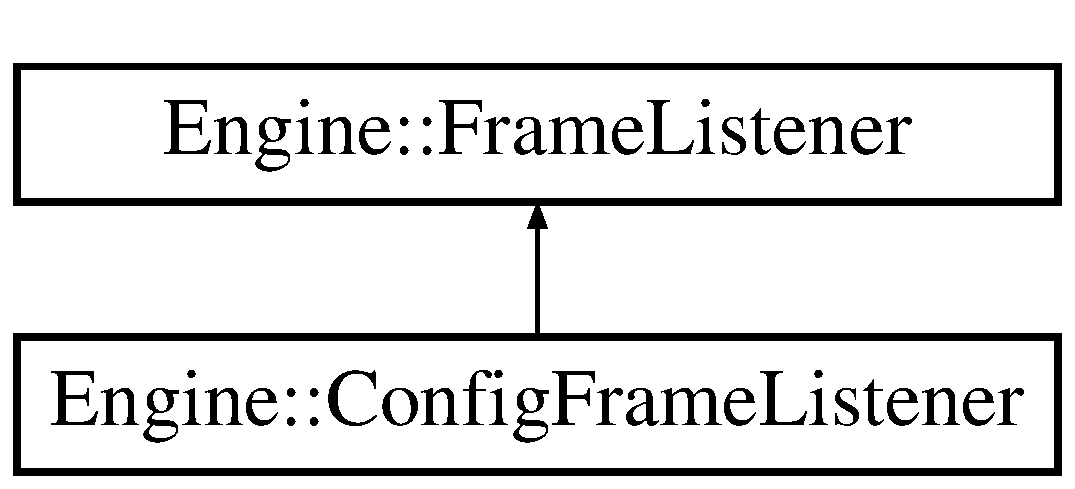
\includegraphics[height=2.000000cm]{classEngine_1_1FrameListener}
\end{center}
\end{figure}
\subsection*{Public Member Functions}
\begin{DoxyCompactItemize}
\item 
virtual void \hyperlink{classEngine_1_1FrameListener_abbe0d745faf156e01d2317b52f29bb48}{initialize} (\hyperlink{classEngine_1_1OpenPolygonDisplay}{Open\+Polygon\+Display} $\ast$display)=0
\begin{DoxyCompactList}\small\item\em initialize \end{DoxyCompactList}\item 
virtual void \hyperlink{classEngine_1_1FrameListener_a3e111a872dd6592c14e11d3280ce14c4}{Render\+Logic} (float time)=0
\begin{DoxyCompactList}\small\item\em Render\+Logic. \end{DoxyCompactList}\end{DoxyCompactItemize}


\subsection{Detailed Description}
The \hyperlink{classEngine_1_1FrameListener}{Frame\+Listener} -\/ Interface class. 

\subsection{Member Function Documentation}
\hypertarget{classEngine_1_1FrameListener_abbe0d745faf156e01d2317b52f29bb48}{}\index{Engine\+::\+Frame\+Listener@{Engine\+::\+Frame\+Listener}!initialize@{initialize}}
\index{initialize@{initialize}!Engine\+::\+Frame\+Listener@{Engine\+::\+Frame\+Listener}}
\subsubsection[{initialize(\+Open\+Polygon\+Display $\ast$display)=0}]{\setlength{\rightskip}{0pt plus 5cm}virtual void Engine\+::\+Frame\+Listener\+::initialize (
\begin{DoxyParamCaption}
\item[{{\bf Open\+Polygon\+Display} $\ast$}]{display}
\end{DoxyParamCaption}
)\hspace{0.3cm}{\ttfamily [pure virtual]}}\label{classEngine_1_1FrameListener_abbe0d745faf156e01d2317b52f29bb48}


initialize 

Initialize Part


\begin{DoxyItemize}
\item create Elements or \hyperlink{classEngine_1_1Entity}{Entity} Objects
\item create a Scene 
\end{DoxyItemize}

Implemented in \hyperlink{classEngine_1_1ConfigFrameListener_a792fe9af553206a358bc888fdc43f2be}{Engine\+::\+Config\+Frame\+Listener}.

\hypertarget{classEngine_1_1FrameListener_a3e111a872dd6592c14e11d3280ce14c4}{}\index{Engine\+::\+Frame\+Listener@{Engine\+::\+Frame\+Listener}!Render\+Logic@{Render\+Logic}}
\index{Render\+Logic@{Render\+Logic}!Engine\+::\+Frame\+Listener@{Engine\+::\+Frame\+Listener}}
\subsubsection[{Render\+Logic(float time)=0}]{\setlength{\rightskip}{0pt plus 5cm}virtual void Engine\+::\+Frame\+Listener\+::\+Render\+Logic (
\begin{DoxyParamCaption}
\item[{float}]{time}
\end{DoxyParamCaption}
)\hspace{0.3cm}{\ttfamily [pure virtual]}}\label{classEngine_1_1FrameListener_a3e111a872dd6592c14e11d3280ce14c4}


Render\+Logic. 

Logic Part


\begin{DoxyItemize}
\item modifier Elements or Entitys
\end{DoxyItemize}


\begin{DoxyParams}{Parameters}
{\em time} & \\
\hline
\end{DoxyParams}


Implemented in \hyperlink{classEngine_1_1ConfigFrameListener_addb569607e5f870efda08a1a7de41544}{Engine\+::\+Config\+Frame\+Listener}.



The documentation for this class was generated from the following file\+:\begin{DoxyCompactItemize}
\item 
include/\+Interface/framelistener.\+h\end{DoxyCompactItemize}

\hypertarget{classEngine_1_1FunctorWorker}{}\section{Engine\+:\+:Functor\+Worker Class Reference}
\label{classEngine_1_1FunctorWorker}\index{Engine\+::\+Functor\+Worker@{Engine\+::\+Functor\+Worker}}


The \hyperlink{classEngine_1_1FunctorWorker}{Functor\+Worker} class.  




{\ttfamily \#include $<$threadmanager.\+h$>$}

\subsection*{Public Member Functions}
\begin{DoxyCompactItemize}
\item 
\hypertarget{classEngine_1_1FunctorWorker_afdf2e47da4345ac76e9d3591d5579dc2}{}virtual void {\bfseries operator()} ()\label{classEngine_1_1FunctorWorker_afdf2e47da4345ac76e9d3591d5579dc2}

\end{DoxyCompactItemize}


\subsection{Detailed Description}
The \hyperlink{classEngine_1_1FunctorWorker}{Functor\+Worker} class. 

\hyperlink{classEngine_1_1FunctorWorker}{Functor\+Worker} a Basis Class 

The documentation for this class was generated from the following files\+:\begin{DoxyCompactItemize}
\item 
include/\+Manager/threadmanager.\+h\item 
Engine/\+Manager/Thread\+Manager.\+cpp\end{DoxyCompactItemize}

\hypertarget{classEngine_1_1GLArrayBuffer}{}\section{Engine\+:\+:G\+L\+Array\+Buffer Class Reference}
\label{classEngine_1_1GLArrayBuffer}\index{Engine\+::\+G\+L\+Array\+Buffer@{Engine\+::\+G\+L\+Array\+Buffer}}


The \hyperlink{classEngine_1_1GLArrayBuffer}{G\+L\+Array\+Buffer} class.  




{\ttfamily \#include $<$glarraybuffer.\+h$>$}

Inheritance diagram for Engine\+:\+:G\+L\+Array\+Buffer\+:\begin{figure}[H]
\begin{center}
\leavevmode
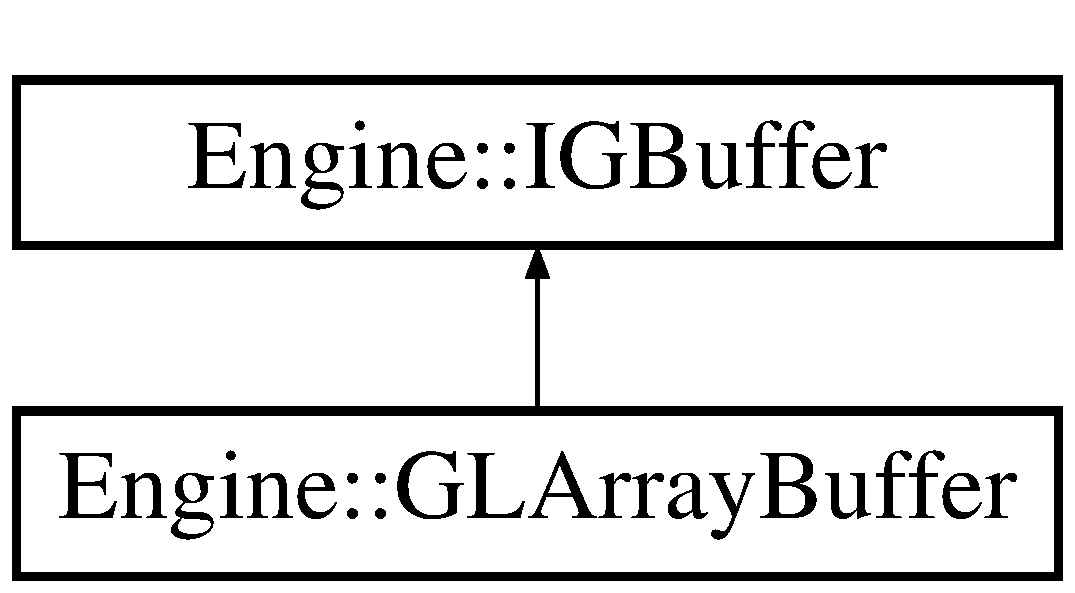
\includegraphics[height=2.000000cm]{classEngine_1_1GLArrayBuffer}
\end{center}
\end{figure}
\subsection*{Public Member Functions}
\begin{DoxyCompactItemize}
\item 
uint \hyperlink{classEngine_1_1GLArrayBuffer_aec618c4096d7b6d2ab39dde5fb55976b}{create} (int size\+\_\+data, void $\ast$data)
\begin{DoxyCompactList}\small\item\em create \end{DoxyCompactList}\item 
void \hyperlink{classEngine_1_1GLArrayBuffer_a5c31588067f1f10c0c9f35aedd8b73af}{attach} (uint vao\+\_\+id)
\begin{DoxyCompactList}\small\item\em attach \end{DoxyCompactList}\item 
\hypertarget{classEngine_1_1GLArrayBuffer_a9b15814cef2ea5ba9021c7637109cf07}{}void {\bfseries update} (int offset, int size\+\_\+data, void $\ast$data)\label{classEngine_1_1GLArrayBuffer_a9b15814cef2ea5ba9021c7637109cf07}

\item 
void \hyperlink{classEngine_1_1GLArrayBuffer_a6ca4905a31d11d291df25abbfe95f177}{get\+Data} (int offset, void $\ast$data)
\begin{DoxyCompactList}\small\item\em get\+Data \end{DoxyCompactList}\item 
void \hyperlink{classEngine_1_1GLArrayBuffer_aa6e0bd973444f5c23bf94fdc88e2e5ca}{close} (void)
\begin{DoxyCompactList}\small\item\em close \end{DoxyCompactList}\end{DoxyCompactItemize}
\subsection*{Additional Inherited Members}


\subsection{Detailed Description}
The \hyperlink{classEngine_1_1GLArrayBuffer}{G\+L\+Array\+Buffer} class. 

\subsection{Member Function Documentation}
\hypertarget{classEngine_1_1GLArrayBuffer_a5c31588067f1f10c0c9f35aedd8b73af}{}\index{Engine\+::\+G\+L\+Array\+Buffer@{Engine\+::\+G\+L\+Array\+Buffer}!attach@{attach}}
\index{attach@{attach}!Engine\+::\+G\+L\+Array\+Buffer@{Engine\+::\+G\+L\+Array\+Buffer}}
\subsubsection[{attach(uint vao\+\_\+id)}]{\setlength{\rightskip}{0pt plus 5cm}void G\+L\+Array\+Buffer\+::attach (
\begin{DoxyParamCaption}
\item[{uint}]{vao\+\_\+id}
\end{DoxyParamCaption}
)\hspace{0.3cm}{\ttfamily [virtual]}}\label{classEngine_1_1GLArrayBuffer_a5c31588067f1f10c0c9f35aedd8b73af}


attach 


\begin{DoxyParams}{Parameters}
{\em vao\+\_\+id} & \\
\hline
\end{DoxyParams}


Implements \hyperlink{classEngine_1_1IGBuffer_a4d4186068930b5d161a52d2fa8afad02}{Engine\+::\+I\+G\+Buffer}.

\hypertarget{classEngine_1_1GLArrayBuffer_aa6e0bd973444f5c23bf94fdc88e2e5ca}{}\index{Engine\+::\+G\+L\+Array\+Buffer@{Engine\+::\+G\+L\+Array\+Buffer}!close@{close}}
\index{close@{close}!Engine\+::\+G\+L\+Array\+Buffer@{Engine\+::\+G\+L\+Array\+Buffer}}
\subsubsection[{close(void)}]{\setlength{\rightskip}{0pt plus 5cm}void G\+L\+Array\+Buffer\+::close (
\begin{DoxyParamCaption}
\item[{void}]{}
\end{DoxyParamCaption}
)\hspace{0.3cm}{\ttfamily [virtual]}}\label{classEngine_1_1GLArrayBuffer_aa6e0bd973444f5c23bf94fdc88e2e5ca}


close 

Unbind G\+P\+U Buffer 

Implements \hyperlink{classEngine_1_1IGBuffer_a8473523f8cf850708f54859848f4234e}{Engine\+::\+I\+G\+Buffer}.

\hypertarget{classEngine_1_1GLArrayBuffer_aec618c4096d7b6d2ab39dde5fb55976b}{}\index{Engine\+::\+G\+L\+Array\+Buffer@{Engine\+::\+G\+L\+Array\+Buffer}!create@{create}}
\index{create@{create}!Engine\+::\+G\+L\+Array\+Buffer@{Engine\+::\+G\+L\+Array\+Buffer}}
\subsubsection[{create(int size\+\_\+data, void $\ast$data)}]{\setlength{\rightskip}{0pt plus 5cm}uint G\+L\+Array\+Buffer\+::create (
\begin{DoxyParamCaption}
\item[{int}]{size\+\_\+data, }
\item[{void $\ast$}]{data}
\end{DoxyParamCaption}
)\hspace{0.3cm}{\ttfamily [virtual]}}\label{classEngine_1_1GLArrayBuffer_aec618c4096d7b6d2ab39dde5fb55976b}


create 

Create a new G\+P\+U Buffer 

Implements \hyperlink{classEngine_1_1IGBuffer_a6afbd1651d2c92fcec584e8d3ef1c32b}{Engine\+::\+I\+G\+Buffer}.

\hypertarget{classEngine_1_1GLArrayBuffer_a6ca4905a31d11d291df25abbfe95f177}{}\index{Engine\+::\+G\+L\+Array\+Buffer@{Engine\+::\+G\+L\+Array\+Buffer}!get\+Data@{get\+Data}}
\index{get\+Data@{get\+Data}!Engine\+::\+G\+L\+Array\+Buffer@{Engine\+::\+G\+L\+Array\+Buffer}}
\subsubsection[{get\+Data(int offset, void $\ast$data)}]{\setlength{\rightskip}{0pt plus 5cm}void G\+L\+Array\+Buffer\+::get\+Data (
\begin{DoxyParamCaption}
\item[{int}]{offset, }
\item[{void $\ast$}]{data}
\end{DoxyParamCaption}
)\hspace{0.3cm}{\ttfamily [virtual]}}\label{classEngine_1_1GLArrayBuffer_a6ca4905a31d11d291df25abbfe95f177}


get\+Data 

Get Data from Buffer 
\begin{DoxyParams}{Parameters}
{\em offset} & \\
\hline
{\em size\+\_\+data} & \\
\hline
\end{DoxyParams}
\begin{DoxyReturn}{Returns}

\end{DoxyReturn}


Implements \hyperlink{classEngine_1_1IGBuffer_a8ad52dc670797d72aabf99033d20b220}{Engine\+::\+I\+G\+Buffer}.



The documentation for this class was generated from the following files\+:\begin{DoxyCompactItemize}
\item 
include/\+G\+P\+U/glarraybuffer.\+h\item 
Engine/\+G\+P\+U/G\+L\+Array\+Buffer.\+cpp\end{DoxyCompactItemize}

\hypertarget{classEngine_1_1GLCustomAttributeBuffer}{}\section{Engine\+:\+:G\+L\+Custom\+Attribute\+Buffer Class Reference}
\label{classEngine_1_1GLCustomAttributeBuffer}\index{Engine\+::\+G\+L\+Custom\+Attribute\+Buffer@{Engine\+::\+G\+L\+Custom\+Attribute\+Buffer}}


The \hyperlink{classEngine_1_1GLCustomAttributeBuffer}{G\+L\+Custom\+Attribute\+Buffer} class.  




{\ttfamily \#include $<$glcustomattributebuffer.\+h$>$}

Inheritance diagram for Engine\+:\+:G\+L\+Custom\+Attribute\+Buffer\+:\begin{figure}[H]
\begin{center}
\leavevmode
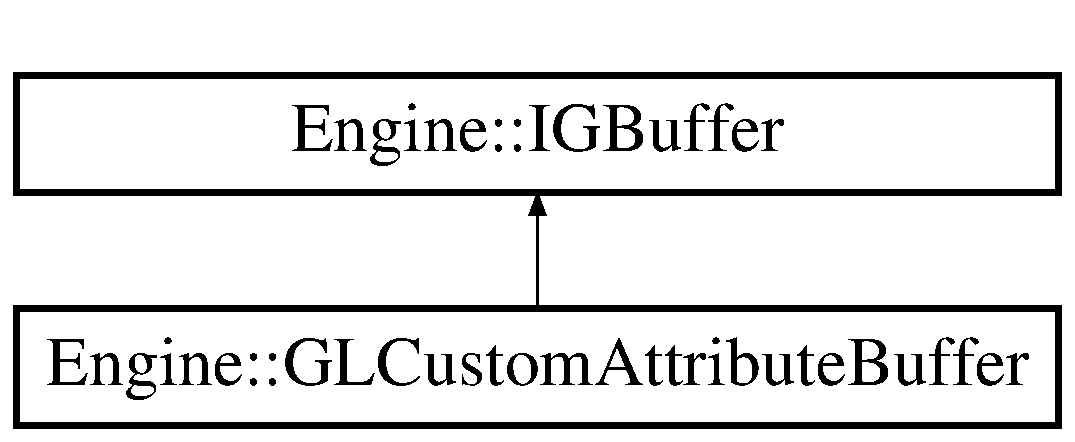
\includegraphics[height=2.000000cm]{classEngine_1_1GLCustomAttributeBuffer}
\end{center}
\end{figure}
\subsection*{Public Member Functions}
\begin{DoxyCompactItemize}
\item 
\hypertarget{classEngine_1_1GLCustomAttributeBuffer_a63094f27c825fef583f86f154d10199e}{}{\bfseries G\+L\+Custom\+Attribute\+Buffer} (uint attribute\+\_\+id, uint type, int vector\+\_\+size, bool instance)\label{classEngine_1_1GLCustomAttributeBuffer_a63094f27c825fef583f86f154d10199e}

\item 
uint \hyperlink{classEngine_1_1GLCustomAttributeBuffer_a41743693090a4ea7d0021f61d80e83a8}{create} (int size\+\_\+data, void $\ast$data)
\begin{DoxyCompactList}\small\item\em create \end{DoxyCompactList}\item 
void \hyperlink{classEngine_1_1GLCustomAttributeBuffer_a0decec64cba335e28acd81268650c3b3}{attach} (uint vao\+\_\+id)
\begin{DoxyCompactList}\small\item\em attach \end{DoxyCompactList}\item 
\hypertarget{classEngine_1_1GLCustomAttributeBuffer_a1ce190cb90d2b46c4524794b2d21a5ca}{}void {\bfseries update} (int offset, int size\+\_\+data, void $\ast$data)\label{classEngine_1_1GLCustomAttributeBuffer_a1ce190cb90d2b46c4524794b2d21a5ca}

\item 
void \hyperlink{classEngine_1_1GLCustomAttributeBuffer_a828a015ce58e25c6422505f0cadfd799}{get\+Data} (int offset, void $\ast$data)
\begin{DoxyCompactList}\small\item\em get\+Data \end{DoxyCompactList}\item 
void \hyperlink{classEngine_1_1GLCustomAttributeBuffer_a84dd56904b35cd71f6a8866c36063f5d}{close} (void)
\begin{DoxyCompactList}\small\item\em close \end{DoxyCompactList}\end{DoxyCompactItemize}
\subsection*{Additional Inherited Members}


\subsection{Detailed Description}
The \hyperlink{classEngine_1_1GLCustomAttributeBuffer}{G\+L\+Custom\+Attribute\+Buffer} class. 

\subsection{Member Function Documentation}
\hypertarget{classEngine_1_1GLCustomAttributeBuffer_a0decec64cba335e28acd81268650c3b3}{}\index{Engine\+::\+G\+L\+Custom\+Attribute\+Buffer@{Engine\+::\+G\+L\+Custom\+Attribute\+Buffer}!attach@{attach}}
\index{attach@{attach}!Engine\+::\+G\+L\+Custom\+Attribute\+Buffer@{Engine\+::\+G\+L\+Custom\+Attribute\+Buffer}}
\subsubsection[{attach(uint vao\+\_\+id)}]{\setlength{\rightskip}{0pt plus 5cm}void G\+L\+Custom\+Attribute\+Buffer\+::attach (
\begin{DoxyParamCaption}
\item[{uint}]{vao\+\_\+id}
\end{DoxyParamCaption}
)\hspace{0.3cm}{\ttfamily [virtual]}}\label{classEngine_1_1GLCustomAttributeBuffer_a0decec64cba335e28acd81268650c3b3}


attach 


\begin{DoxyParams}{Parameters}
{\em vao\+\_\+id} & \\
\hline
\end{DoxyParams}


Implements \hyperlink{classEngine_1_1IGBuffer_a4d4186068930b5d161a52d2fa8afad02}{Engine\+::\+I\+G\+Buffer}.

\hypertarget{classEngine_1_1GLCustomAttributeBuffer_a84dd56904b35cd71f6a8866c36063f5d}{}\index{Engine\+::\+G\+L\+Custom\+Attribute\+Buffer@{Engine\+::\+G\+L\+Custom\+Attribute\+Buffer}!close@{close}}
\index{close@{close}!Engine\+::\+G\+L\+Custom\+Attribute\+Buffer@{Engine\+::\+G\+L\+Custom\+Attribute\+Buffer}}
\subsubsection[{close(void)}]{\setlength{\rightskip}{0pt plus 5cm}void G\+L\+Custom\+Attribute\+Buffer\+::close (
\begin{DoxyParamCaption}
\item[{void}]{}
\end{DoxyParamCaption}
)\hspace{0.3cm}{\ttfamily [virtual]}}\label{classEngine_1_1GLCustomAttributeBuffer_a84dd56904b35cd71f6a8866c36063f5d}


close 

Unbind G\+P\+U Buffer 

Implements \hyperlink{classEngine_1_1IGBuffer_a8473523f8cf850708f54859848f4234e}{Engine\+::\+I\+G\+Buffer}.

\hypertarget{classEngine_1_1GLCustomAttributeBuffer_a41743693090a4ea7d0021f61d80e83a8}{}\index{Engine\+::\+G\+L\+Custom\+Attribute\+Buffer@{Engine\+::\+G\+L\+Custom\+Attribute\+Buffer}!create@{create}}
\index{create@{create}!Engine\+::\+G\+L\+Custom\+Attribute\+Buffer@{Engine\+::\+G\+L\+Custom\+Attribute\+Buffer}}
\subsubsection[{create(int size\+\_\+data, void $\ast$data)}]{\setlength{\rightskip}{0pt plus 5cm}uint G\+L\+Custom\+Attribute\+Buffer\+::create (
\begin{DoxyParamCaption}
\item[{int}]{size\+\_\+data, }
\item[{void $\ast$}]{data}
\end{DoxyParamCaption}
)\hspace{0.3cm}{\ttfamily [virtual]}}\label{classEngine_1_1GLCustomAttributeBuffer_a41743693090a4ea7d0021f61d80e83a8}


create 

Create a new G\+P\+U Buffer 

Implements \hyperlink{classEngine_1_1IGBuffer_a6afbd1651d2c92fcec584e8d3ef1c32b}{Engine\+::\+I\+G\+Buffer}.

\hypertarget{classEngine_1_1GLCustomAttributeBuffer_a828a015ce58e25c6422505f0cadfd799}{}\index{Engine\+::\+G\+L\+Custom\+Attribute\+Buffer@{Engine\+::\+G\+L\+Custom\+Attribute\+Buffer}!get\+Data@{get\+Data}}
\index{get\+Data@{get\+Data}!Engine\+::\+G\+L\+Custom\+Attribute\+Buffer@{Engine\+::\+G\+L\+Custom\+Attribute\+Buffer}}
\subsubsection[{get\+Data(int offset, void $\ast$data)}]{\setlength{\rightskip}{0pt plus 5cm}void G\+L\+Custom\+Attribute\+Buffer\+::get\+Data (
\begin{DoxyParamCaption}
\item[{int}]{offset, }
\item[{void $\ast$}]{data}
\end{DoxyParamCaption}
)\hspace{0.3cm}{\ttfamily [virtual]}}\label{classEngine_1_1GLCustomAttributeBuffer_a828a015ce58e25c6422505f0cadfd799}


get\+Data 

Get Data from Buffer 
\begin{DoxyParams}{Parameters}
{\em offset} & \\
\hline
{\em size\+\_\+data} & \\
\hline
\end{DoxyParams}
\begin{DoxyReturn}{Returns}

\end{DoxyReturn}


Implements \hyperlink{classEngine_1_1IGBuffer_a8ad52dc670797d72aabf99033d20b220}{Engine\+::\+I\+G\+Buffer}.



The documentation for this class was generated from the following files\+:\begin{DoxyCompactItemize}
\item 
include/\+G\+P\+U/glcustomattributebuffer.\+h\item 
Engine/\+G\+P\+U/G\+L\+Custom\+Attribute\+Buffer.\+cpp\end{DoxyCompactItemize}

\hypertarget{classEngine_1_1GLElementBuffer}{}\section{Engine\+:\+:G\+L\+Element\+Buffer Class Reference}
\label{classEngine_1_1GLElementBuffer}\index{Engine\+::\+G\+L\+Element\+Buffer@{Engine\+::\+G\+L\+Element\+Buffer}}


The \hyperlink{classEngine_1_1GLElementBuffer}{G\+L\+Element\+Buffer} class.  




{\ttfamily \#include $<$glelementbuffer.\+h$>$}

Inheritance diagram for Engine\+:\+:G\+L\+Element\+Buffer\+:\begin{figure}[H]
\begin{center}
\leavevmode
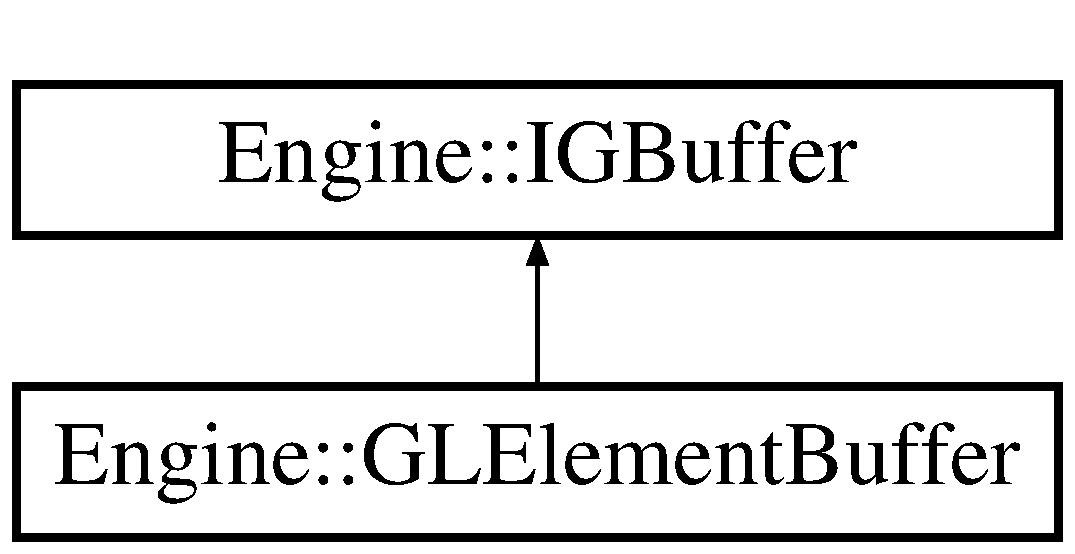
\includegraphics[height=2.000000cm]{classEngine_1_1GLElementBuffer}
\end{center}
\end{figure}
\subsection*{Public Member Functions}
\begin{DoxyCompactItemize}
\item 
uint \hyperlink{classEngine_1_1GLElementBuffer_a36ddf0be23d19af69b60b0a1502768c5}{create} (int size\+\_\+data, void $\ast$data)
\begin{DoxyCompactList}\small\item\em create \end{DoxyCompactList}\item 
void \hyperlink{classEngine_1_1GLElementBuffer_a12e74567261194e53b9b58b52ff91da4}{attach} (uint vao\+\_\+id)
\begin{DoxyCompactList}\small\item\em attach \end{DoxyCompactList}\item 
\hypertarget{classEngine_1_1GLElementBuffer_a1128832938db430f2cb97e3e18d66cac}{}void {\bfseries update} (int offset, int size\+\_\+data, void $\ast$data)\label{classEngine_1_1GLElementBuffer_a1128832938db430f2cb97e3e18d66cac}

\item 
void \hyperlink{classEngine_1_1GLElementBuffer_a78842b1b2910f198665096b72186a1be}{get\+Data} (int offset, void $\ast$data)
\begin{DoxyCompactList}\small\item\em get\+Data \end{DoxyCompactList}\item 
void \hyperlink{classEngine_1_1GLElementBuffer_a8d46099a8a43d1ac1217e765863997ea}{close} (void)
\begin{DoxyCompactList}\small\item\em close \end{DoxyCompactList}\item 
\hypertarget{classEngine_1_1GLElementBuffer_a24aea14bff4e6ac3d34d06d2132d34f2}{}int {\bfseries get\+Float\+Count} (void)\label{classEngine_1_1GLElementBuffer_a24aea14bff4e6ac3d34d06d2132d34f2}

\item 
\hypertarget{classEngine_1_1GLElementBuffer_aa864f1bbd2aba4cd327b0e8a485fceb5}{}void {\bfseries set\+Float\+Count} (int amount)\label{classEngine_1_1GLElementBuffer_aa864f1bbd2aba4cd327b0e8a485fceb5}

\end{DoxyCompactItemize}
\subsection*{Additional Inherited Members}


\subsection{Detailed Description}
The \hyperlink{classEngine_1_1GLElementBuffer}{G\+L\+Element\+Buffer} class. 

\subsection{Member Function Documentation}
\hypertarget{classEngine_1_1GLElementBuffer_a12e74567261194e53b9b58b52ff91da4}{}\index{Engine\+::\+G\+L\+Element\+Buffer@{Engine\+::\+G\+L\+Element\+Buffer}!attach@{attach}}
\index{attach@{attach}!Engine\+::\+G\+L\+Element\+Buffer@{Engine\+::\+G\+L\+Element\+Buffer}}
\subsubsection[{attach(uint vao\+\_\+id)}]{\setlength{\rightskip}{0pt plus 5cm}void G\+L\+Element\+Buffer\+::attach (
\begin{DoxyParamCaption}
\item[{uint}]{vao\+\_\+id}
\end{DoxyParamCaption}
)\hspace{0.3cm}{\ttfamily [virtual]}}\label{classEngine_1_1GLElementBuffer_a12e74567261194e53b9b58b52ff91da4}


attach 


\begin{DoxyParams}{Parameters}
{\em vao\+\_\+id} & \\
\hline
\end{DoxyParams}


Implements \hyperlink{classEngine_1_1IGBuffer_a4d4186068930b5d161a52d2fa8afad02}{Engine\+::\+I\+G\+Buffer}.

\hypertarget{classEngine_1_1GLElementBuffer_a8d46099a8a43d1ac1217e765863997ea}{}\index{Engine\+::\+G\+L\+Element\+Buffer@{Engine\+::\+G\+L\+Element\+Buffer}!close@{close}}
\index{close@{close}!Engine\+::\+G\+L\+Element\+Buffer@{Engine\+::\+G\+L\+Element\+Buffer}}
\subsubsection[{close(void)}]{\setlength{\rightskip}{0pt plus 5cm}void G\+L\+Element\+Buffer\+::close (
\begin{DoxyParamCaption}
\item[{void}]{}
\end{DoxyParamCaption}
)\hspace{0.3cm}{\ttfamily [virtual]}}\label{classEngine_1_1GLElementBuffer_a8d46099a8a43d1ac1217e765863997ea}


close 

Unbind G\+P\+U Buffer 

Implements \hyperlink{classEngine_1_1IGBuffer_a8473523f8cf850708f54859848f4234e}{Engine\+::\+I\+G\+Buffer}.

\hypertarget{classEngine_1_1GLElementBuffer_a36ddf0be23d19af69b60b0a1502768c5}{}\index{Engine\+::\+G\+L\+Element\+Buffer@{Engine\+::\+G\+L\+Element\+Buffer}!create@{create}}
\index{create@{create}!Engine\+::\+G\+L\+Element\+Buffer@{Engine\+::\+G\+L\+Element\+Buffer}}
\subsubsection[{create(int size\+\_\+data, void $\ast$data)}]{\setlength{\rightskip}{0pt plus 5cm}uint G\+L\+Element\+Buffer\+::create (
\begin{DoxyParamCaption}
\item[{int}]{size\+\_\+data, }
\item[{void $\ast$}]{data}
\end{DoxyParamCaption}
)\hspace{0.3cm}{\ttfamily [virtual]}}\label{classEngine_1_1GLElementBuffer_a36ddf0be23d19af69b60b0a1502768c5}


create 

Create a new G\+P\+U Buffer 

Implements \hyperlink{classEngine_1_1IGBuffer_a6afbd1651d2c92fcec584e8d3ef1c32b}{Engine\+::\+I\+G\+Buffer}.

\hypertarget{classEngine_1_1GLElementBuffer_a78842b1b2910f198665096b72186a1be}{}\index{Engine\+::\+G\+L\+Element\+Buffer@{Engine\+::\+G\+L\+Element\+Buffer}!get\+Data@{get\+Data}}
\index{get\+Data@{get\+Data}!Engine\+::\+G\+L\+Element\+Buffer@{Engine\+::\+G\+L\+Element\+Buffer}}
\subsubsection[{get\+Data(int offset, void $\ast$data)}]{\setlength{\rightskip}{0pt plus 5cm}void G\+L\+Element\+Buffer\+::get\+Data (
\begin{DoxyParamCaption}
\item[{int}]{offset, }
\item[{void $\ast$}]{data}
\end{DoxyParamCaption}
)\hspace{0.3cm}{\ttfamily [virtual]}}\label{classEngine_1_1GLElementBuffer_a78842b1b2910f198665096b72186a1be}


get\+Data 

Get Data from Buffer 
\begin{DoxyParams}{Parameters}
{\em offset} & \\
\hline
{\em size\+\_\+data} & \\
\hline
\end{DoxyParams}
\begin{DoxyReturn}{Returns}

\end{DoxyReturn}


Implements \hyperlink{classEngine_1_1IGBuffer_a8ad52dc670797d72aabf99033d20b220}{Engine\+::\+I\+G\+Buffer}.



The documentation for this class was generated from the following files\+:\begin{DoxyCompactItemize}
\item 
include/\+G\+P\+U/glelementbuffer.\+h\item 
Engine/\+G\+P\+U/G\+L\+Element\+Buffer.\+cpp\end{DoxyCompactItemize}

\hypertarget{classEngine_1_1GLFeedbackBuffer}{}\section{Engine\+:\+:G\+L\+Feedback\+Buffer Class Reference}
\label{classEngine_1_1GLFeedbackBuffer}\index{Engine\+::\+G\+L\+Feedback\+Buffer@{Engine\+::\+G\+L\+Feedback\+Buffer}}


The \hyperlink{classEngine_1_1GLFeedbackBuffer}{G\+L\+Feedback\+Buffer} class.  




{\ttfamily \#include $<$glfeedbackbuffer.\+h$>$}

Inheritance diagram for Engine\+:\+:G\+L\+Feedback\+Buffer\+:\begin{figure}[H]
\begin{center}
\leavevmode
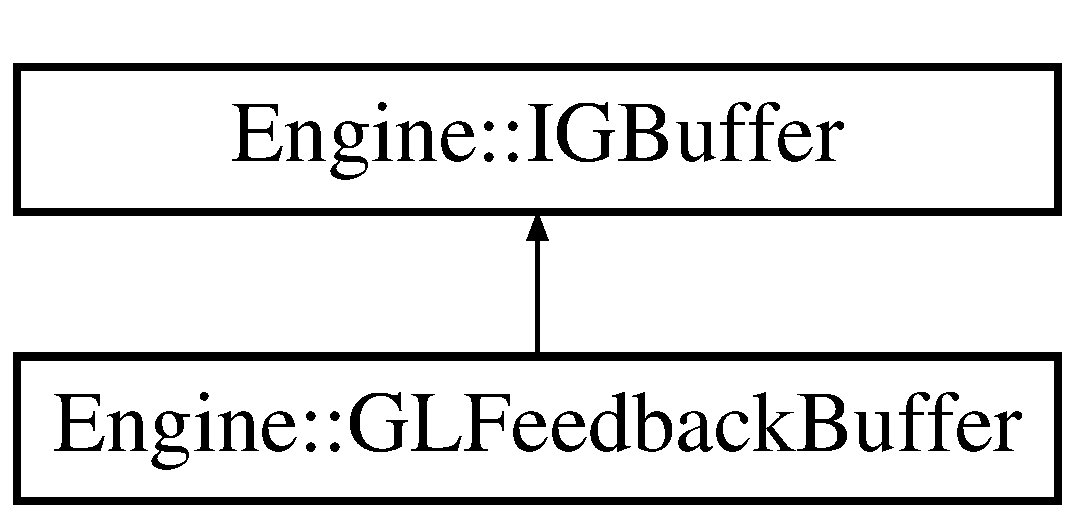
\includegraphics[height=2.000000cm]{classEngine_1_1GLFeedbackBuffer}
\end{center}
\end{figure}
\subsection*{Public Member Functions}
\begin{DoxyCompactItemize}
\item 
uint \hyperlink{classEngine_1_1GLFeedbackBuffer_af07b1ef217ec8a8c77412fe417564428}{create} (int size\+\_\+data, void $\ast$data)
\begin{DoxyCompactList}\small\item\em create \end{DoxyCompactList}\item 
void \hyperlink{classEngine_1_1GLFeedbackBuffer_ae1d18bd14a843d4fcd030998498128c6}{attach} (uint vao\+\_\+id)
\begin{DoxyCompactList}\small\item\em attach \end{DoxyCompactList}\item 
\hypertarget{classEngine_1_1GLFeedbackBuffer_ac37c720e82875e06707e0d4c5c2dc3c0}{}void {\bfseries update} (int offset, int size\+\_\+data, void $\ast$data)\label{classEngine_1_1GLFeedbackBuffer_ac37c720e82875e06707e0d4c5c2dc3c0}

\item 
void \hyperlink{classEngine_1_1GLFeedbackBuffer_a8c4b82243c6652f377d7511ade32e7b5}{get\+Data} (int offset, void $\ast$data)
\begin{DoxyCompactList}\small\item\em get\+Data \end{DoxyCompactList}\item 
void \hyperlink{classEngine_1_1GLFeedbackBuffer_a278dd1fdb1b2fe62a30b7711ea1090a2}{close} (void)
\begin{DoxyCompactList}\small\item\em close \end{DoxyCompactList}\end{DoxyCompactItemize}
\subsection*{Additional Inherited Members}


\subsection{Detailed Description}
The \hyperlink{classEngine_1_1GLFeedbackBuffer}{G\+L\+Feedback\+Buffer} class. 

\subsection{Member Function Documentation}
\hypertarget{classEngine_1_1GLFeedbackBuffer_ae1d18bd14a843d4fcd030998498128c6}{}\index{Engine\+::\+G\+L\+Feedback\+Buffer@{Engine\+::\+G\+L\+Feedback\+Buffer}!attach@{attach}}
\index{attach@{attach}!Engine\+::\+G\+L\+Feedback\+Buffer@{Engine\+::\+G\+L\+Feedback\+Buffer}}
\subsubsection[{attach(uint vao\+\_\+id)}]{\setlength{\rightskip}{0pt plus 5cm}void G\+L\+Feedback\+Buffer\+::attach (
\begin{DoxyParamCaption}
\item[{uint}]{vao\+\_\+id}
\end{DoxyParamCaption}
)\hspace{0.3cm}{\ttfamily [virtual]}}\label{classEngine_1_1GLFeedbackBuffer_ae1d18bd14a843d4fcd030998498128c6}


attach 


\begin{DoxyParams}{Parameters}
{\em vao\+\_\+id} & \\
\hline
\end{DoxyParams}


Implements \hyperlink{classEngine_1_1IGBuffer_a4d4186068930b5d161a52d2fa8afad02}{Engine\+::\+I\+G\+Buffer}.

\hypertarget{classEngine_1_1GLFeedbackBuffer_a278dd1fdb1b2fe62a30b7711ea1090a2}{}\index{Engine\+::\+G\+L\+Feedback\+Buffer@{Engine\+::\+G\+L\+Feedback\+Buffer}!close@{close}}
\index{close@{close}!Engine\+::\+G\+L\+Feedback\+Buffer@{Engine\+::\+G\+L\+Feedback\+Buffer}}
\subsubsection[{close(void)}]{\setlength{\rightskip}{0pt plus 5cm}void G\+L\+Feedback\+Buffer\+::close (
\begin{DoxyParamCaption}
\item[{void}]{}
\end{DoxyParamCaption}
)\hspace{0.3cm}{\ttfamily [virtual]}}\label{classEngine_1_1GLFeedbackBuffer_a278dd1fdb1b2fe62a30b7711ea1090a2}


close 

Unbind G\+P\+U Buffer 

Implements \hyperlink{classEngine_1_1IGBuffer_a8473523f8cf850708f54859848f4234e}{Engine\+::\+I\+G\+Buffer}.

\hypertarget{classEngine_1_1GLFeedbackBuffer_af07b1ef217ec8a8c77412fe417564428}{}\index{Engine\+::\+G\+L\+Feedback\+Buffer@{Engine\+::\+G\+L\+Feedback\+Buffer}!create@{create}}
\index{create@{create}!Engine\+::\+G\+L\+Feedback\+Buffer@{Engine\+::\+G\+L\+Feedback\+Buffer}}
\subsubsection[{create(int size\+\_\+data, void $\ast$data)}]{\setlength{\rightskip}{0pt plus 5cm}uint G\+L\+Feedback\+Buffer\+::create (
\begin{DoxyParamCaption}
\item[{int}]{size\+\_\+data, }
\item[{void $\ast$}]{data}
\end{DoxyParamCaption}
)\hspace{0.3cm}{\ttfamily [virtual]}}\label{classEngine_1_1GLFeedbackBuffer_af07b1ef217ec8a8c77412fe417564428}


create 

Create a new G\+P\+U Buffer 

Implements \hyperlink{classEngine_1_1IGBuffer_a6afbd1651d2c92fcec584e8d3ef1c32b}{Engine\+::\+I\+G\+Buffer}.

\hypertarget{classEngine_1_1GLFeedbackBuffer_a8c4b82243c6652f377d7511ade32e7b5}{}\index{Engine\+::\+G\+L\+Feedback\+Buffer@{Engine\+::\+G\+L\+Feedback\+Buffer}!get\+Data@{get\+Data}}
\index{get\+Data@{get\+Data}!Engine\+::\+G\+L\+Feedback\+Buffer@{Engine\+::\+G\+L\+Feedback\+Buffer}}
\subsubsection[{get\+Data(int offset, void $\ast$data)}]{\setlength{\rightskip}{0pt plus 5cm}void G\+L\+Feedback\+Buffer\+::get\+Data (
\begin{DoxyParamCaption}
\item[{int}]{offset, }
\item[{void $\ast$}]{data}
\end{DoxyParamCaption}
)\hspace{0.3cm}{\ttfamily [virtual]}}\label{classEngine_1_1GLFeedbackBuffer_a8c4b82243c6652f377d7511ade32e7b5}


get\+Data 

Get Data from Buffer 
\begin{DoxyParams}{Parameters}
{\em offset} & \\
\hline
{\em size\+\_\+data} & \\
\hline
\end{DoxyParams}
\begin{DoxyReturn}{Returns}

\end{DoxyReturn}


Implements \hyperlink{classEngine_1_1IGBuffer_a8ad52dc670797d72aabf99033d20b220}{Engine\+::\+I\+G\+Buffer}.



The documentation for this class was generated from the following files\+:\begin{DoxyCompactItemize}
\item 
include/\+G\+P\+U/glfeedbackbuffer.\+h\item 
Engine/\+G\+P\+U/G\+L\+Feedback\+Buffer.\+cpp\end{DoxyCompactItemize}

\hypertarget{classEngine_1_1GLFeedbackDoubleBuffer}{}\section{Engine\+:\+:G\+L\+Feedback\+Double\+Buffer Class Reference}
\label{classEngine_1_1GLFeedbackDoubleBuffer}\index{Engine\+::\+G\+L\+Feedback\+Double\+Buffer@{Engine\+::\+G\+L\+Feedback\+Double\+Buffer}}


The \hyperlink{classEngine_1_1GLFeedbackDoubleBuffer}{G\+L\+Feedback\+Double\+Buffer} class.  




{\ttfamily \#include $<$glfeedbackdoublebuffer.\+h$>$}

Inheritance diagram for Engine\+:\+:G\+L\+Feedback\+Double\+Buffer\+:\begin{figure}[H]
\begin{center}
\leavevmode
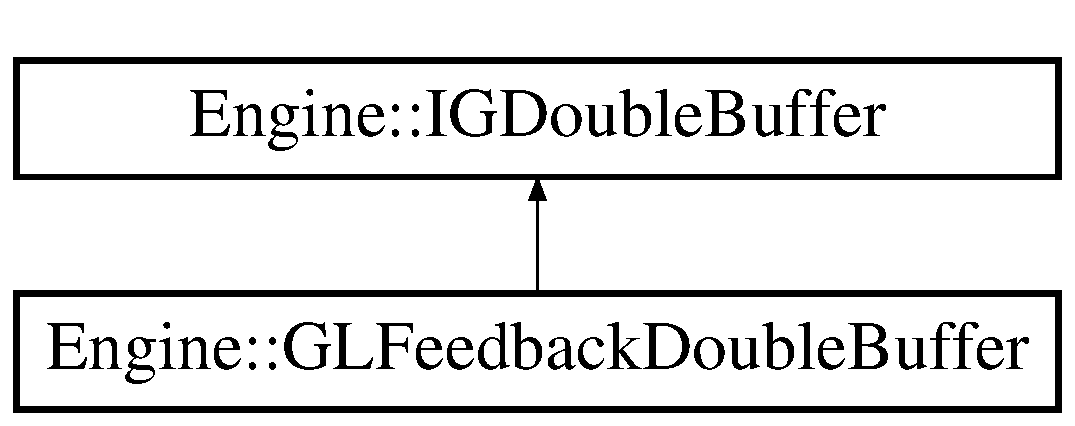
\includegraphics[height=2.000000cm]{classEngine_1_1GLFeedbackDoubleBuffer}
\end{center}
\end{figure}
\subsection*{Public Member Functions}
\begin{DoxyCompactItemize}
\item 
void \hyperlink{classEngine_1_1GLFeedbackDoubleBuffer_a093faa032cd6f229c6a0e6b18fca11b6}{create} (\hyperlink{classEngine_1_1IGBuffer}{I\+G\+Buffer} $\ast$front, \hyperlink{classEngine_1_1IGBuffer}{I\+G\+Buffer} $\ast$back, int size\+\_\+data)
\begin{DoxyCompactList}\small\item\em create \end{DoxyCompactList}\item 
void \hyperlink{classEngine_1_1GLFeedbackDoubleBuffer_a94805048c8b23cb2bf83d40ace22c9cd}{update} (int offset, int size\+\_\+data, void $\ast$data)
\begin{DoxyCompactList}\small\item\em update \end{DoxyCompactList}\item 
void \hyperlink{classEngine_1_1GLFeedbackDoubleBuffer_aee224416eeeaa26f4c1eb0158cde1f68}{Swap\+Buffers} (void)
\begin{DoxyCompactList}\small\item\em Swap\+Buffers. \end{DoxyCompactList}\end{DoxyCompactItemize}
\subsection*{Additional Inherited Members}


\subsection{Detailed Description}
The \hyperlink{classEngine_1_1GLFeedbackDoubleBuffer}{G\+L\+Feedback\+Double\+Buffer} class. 

\subsection{Member Function Documentation}
\hypertarget{classEngine_1_1GLFeedbackDoubleBuffer_a093faa032cd6f229c6a0e6b18fca11b6}{}\index{Engine\+::\+G\+L\+Feedback\+Double\+Buffer@{Engine\+::\+G\+L\+Feedback\+Double\+Buffer}!create@{create}}
\index{create@{create}!Engine\+::\+G\+L\+Feedback\+Double\+Buffer@{Engine\+::\+G\+L\+Feedback\+Double\+Buffer}}
\subsubsection[{create(\+I\+G\+Buffer $\ast$front, I\+G\+Buffer $\ast$back, int size\+\_\+data)}]{\setlength{\rightskip}{0pt plus 5cm}void G\+L\+Feedback\+Double\+Buffer\+::create (
\begin{DoxyParamCaption}
\item[{{\bf I\+G\+Buffer} $\ast$}]{front, }
\item[{{\bf I\+G\+Buffer} $\ast$}]{back, }
\item[{int}]{size\+\_\+data}
\end{DoxyParamCaption}
)\hspace{0.3cm}{\ttfamily [virtual]}}\label{classEngine_1_1GLFeedbackDoubleBuffer_a093faa032cd6f229c6a0e6b18fca11b6}


create 

Create Front and Back Buffer 

Implements \hyperlink{classEngine_1_1IGDoubleBuffer_a094e87543bb24956ec1fd3835b4ca413}{Engine\+::\+I\+G\+Double\+Buffer}.

\hypertarget{classEngine_1_1GLFeedbackDoubleBuffer_aee224416eeeaa26f4c1eb0158cde1f68}{}\index{Engine\+::\+G\+L\+Feedback\+Double\+Buffer@{Engine\+::\+G\+L\+Feedback\+Double\+Buffer}!Swap\+Buffers@{Swap\+Buffers}}
\index{Swap\+Buffers@{Swap\+Buffers}!Engine\+::\+G\+L\+Feedback\+Double\+Buffer@{Engine\+::\+G\+L\+Feedback\+Double\+Buffer}}
\subsubsection[{Swap\+Buffers(void)}]{\setlength{\rightskip}{0pt plus 5cm}void G\+L\+Feedback\+Double\+Buffer\+::\+Swap\+Buffers (
\begin{DoxyParamCaption}
\item[{void}]{}
\end{DoxyParamCaption}
)\hspace{0.3cm}{\ttfamily [virtual]}}\label{classEngine_1_1GLFeedbackDoubleBuffer_aee224416eeeaa26f4c1eb0158cde1f68}


Swap\+Buffers. 

Copy Back buffer data into Front buffer 

Implements \hyperlink{classEngine_1_1IGDoubleBuffer_ade7c5ce0b5883c55f5e66588dd8b14da}{Engine\+::\+I\+G\+Double\+Buffer}.

\hypertarget{classEngine_1_1GLFeedbackDoubleBuffer_a94805048c8b23cb2bf83d40ace22c9cd}{}\index{Engine\+::\+G\+L\+Feedback\+Double\+Buffer@{Engine\+::\+G\+L\+Feedback\+Double\+Buffer}!update@{update}}
\index{update@{update}!Engine\+::\+G\+L\+Feedback\+Double\+Buffer@{Engine\+::\+G\+L\+Feedback\+Double\+Buffer}}
\subsubsection[{update(int offset, int size\+\_\+data, void $\ast$data)}]{\setlength{\rightskip}{0pt plus 5cm}void G\+L\+Feedback\+Double\+Buffer\+::update (
\begin{DoxyParamCaption}
\item[{int}]{offset, }
\item[{int}]{size\+\_\+data, }
\item[{void $\ast$}]{data}
\end{DoxyParamCaption}
)\hspace{0.3cm}{\ttfamily [virtual]}}\label{classEngine_1_1GLFeedbackDoubleBuffer_a94805048c8b23cb2bf83d40ace22c9cd}


update 

Update Back Buffer 
\begin{DoxyParams}{Parameters}
{\em offset} & \\
\hline
{\em size\+\_\+data} & \\
\hline
{\em data} & \\
\hline
\end{DoxyParams}


Implements \hyperlink{classEngine_1_1IGDoubleBuffer_a39b0608ee6f5ddbf14dbea9030b881d8}{Engine\+::\+I\+G\+Double\+Buffer}.



The documentation for this class was generated from the following files\+:\begin{DoxyCompactItemize}
\item 
include/\+G\+P\+U/glfeedbackdoublebuffer.\+h\item 
Engine/\+G\+P\+U/G\+L\+Feedback\+Double\+Buffer.\+cpp\end{DoxyCompactItemize}

\hypertarget{structEngine_1_1GLFWData}{}\section{Engine\+:\+:G\+L\+F\+W\+Data Struct Reference}
\label{structEngine_1_1GLFWData}\index{Engine\+::\+G\+L\+F\+W\+Data@{Engine\+::\+G\+L\+F\+W\+Data}}


The \hyperlink{structEngine_1_1GLFWData}{G\+L\+F\+W\+Data} struct.  




{\ttfamily \#include $<$display.\+h$>$}

\subsection*{Public Attributes}
\begin{DoxyCompactItemize}
\item 
\hypertarget{structEngine_1_1GLFWData_aff9f44d9e271c5a755ff9cdec7de5630}{}G\+L\+F\+Wwindow $\ast$ {\bfseries window}\label{structEngine_1_1GLFWData_aff9f44d9e271c5a755ff9cdec7de5630}

\item 
\hypertarget{structEngine_1_1GLFWData_acbc36b766597db26d5c1536fc8f13575}{}bool {\bfseries mouse\+\_\+visible}\label{structEngine_1_1GLFWData_acbc36b766597db26d5c1536fc8f13575}

\end{DoxyCompactItemize}


\subsection{Detailed Description}
The \hyperlink{structEngine_1_1GLFWData}{G\+L\+F\+W\+Data} struct. 

The documentation for this struct was generated from the following file\+:\begin{DoxyCompactItemize}
\item 
include/\+Container/display.\+h\end{DoxyCompactItemize}

\hypertarget{classEngine_1_1GLFWDisplay}{}\section{Engine\+:\+:G\+L\+F\+W\+Display Class Reference}
\label{classEngine_1_1GLFWDisplay}\index{Engine\+::\+G\+L\+F\+W\+Display@{Engine\+::\+G\+L\+F\+W\+Display}}


The \hyperlink{classEngine_1_1GLFWDisplay}{G\+L\+F\+W\+Display} -\/ display class.  




{\ttfamily \#include $<$display.\+h$>$}

Inheritance diagram for Engine\+:\+:G\+L\+F\+W\+Display\+:\begin{figure}[H]
\begin{center}
\leavevmode
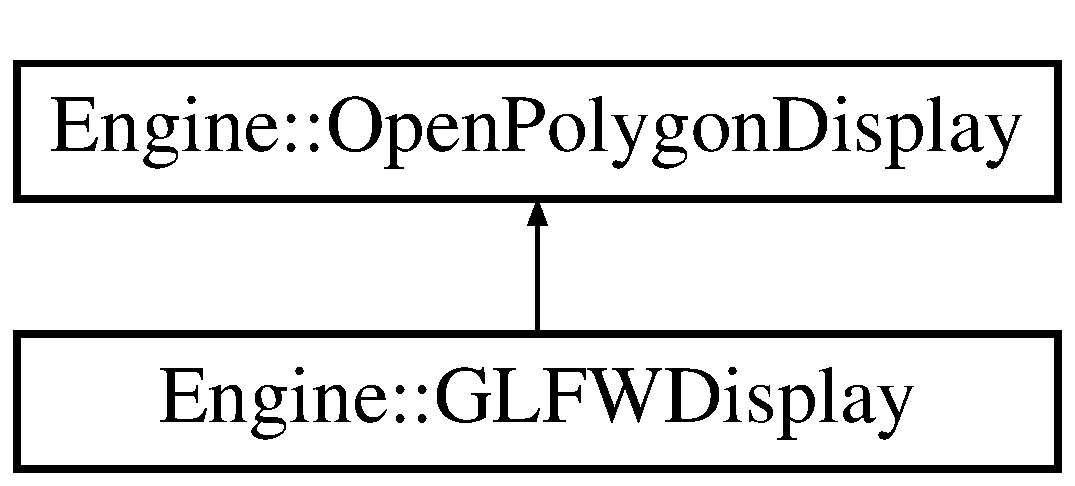
\includegraphics[height=2.000000cm]{classEngine_1_1GLFWDisplay}
\end{center}
\end{figure}
\subsection*{Public Member Functions}
\begin{DoxyCompactItemize}
\item 
\hypertarget{classEngine_1_1GLFWDisplay_a11e7737d66dce9a3fef33f1f5a1b27d1}{}{\bfseries G\+L\+F\+W\+Display} (const std\+::string \&display\+\_\+name)\label{classEngine_1_1GLFWDisplay_a11e7737d66dce9a3fef33f1f5a1b27d1}

\item 
\hypertarget{classEngine_1_1GLFWDisplay_a5a53cf7631695c18aae7c3c3c37d7c5c}{}void {\bfseries Close} (void) final override\label{classEngine_1_1GLFWDisplay_a5a53cf7631695c18aae7c3c3c37d7c5c}

\item 
\hypertarget{classEngine_1_1GLFWDisplay_a138fce031afc06d204121da1ed3c38dd}{}bool {\bfseries is\+Closed} (void) final override\label{classEngine_1_1GLFWDisplay_a138fce031afc06d204121da1ed3c38dd}

\item 
\hypertarget{classEngine_1_1GLFWDisplay_ac2e1863cd5500dfc43199c25a49a2e1d}{}void {\bfseries Update} (void) final override\label{classEngine_1_1GLFWDisplay_ac2e1863cd5500dfc43199c25a49a2e1d}

\item 
\hypertarget{classEngine_1_1GLFWDisplay_acef361f485ccbba0a7347f675b58c09a}{}void {\bfseries set\+Title} (const char $\ast$title) final override\label{classEngine_1_1GLFWDisplay_acef361f485ccbba0a7347f675b58c09a}

\item 
\hypertarget{classEngine_1_1GLFWDisplay_aee19c00f6e759b8f841b946af479221f}{}void {\bfseries set\+Window} (G\+L\+F\+Wwindow $\ast$window)\label{classEngine_1_1GLFWDisplay_aee19c00f6e759b8f841b946af479221f}

\item 
\hypertarget{classEngine_1_1GLFWDisplay_adb15f8359bdfc47eb50efca684b50736}{}void {\bfseries set\+Window\+Size} (int width, int height)\label{classEngine_1_1GLFWDisplay_adb15f8359bdfc47eb50efca684b50736}

\item 
\hypertarget{classEngine_1_1GLFWDisplay_a2e38e41b57d87995372ecbe01211dc52}{}void {\bfseries catch\+Mouse} (bool visible)\label{classEngine_1_1GLFWDisplay_a2e38e41b57d87995372ecbe01211dc52}

\item 
\hypertarget{classEngine_1_1GLFWDisplay_a5b613b17c2aa0537158d57746c0f4d43}{}G\+L\+F\+Wwindow $\ast$ {\bfseries get\+Window} (void)\label{classEngine_1_1GLFWDisplay_a5b613b17c2aa0537158d57746c0f4d43}

\end{DoxyCompactItemize}
\subsection*{Additional Inherited Members}


\subsection{Detailed Description}
The \hyperlink{classEngine_1_1GLFWDisplay}{G\+L\+F\+W\+Display} -\/ display class. 

The documentation for this class was generated from the following files\+:\begin{DoxyCompactItemize}
\item 
include/\+Container/display.\+h\item 
Container/Display.\+cpp\end{DoxyCompactItemize}

\hypertarget{classEngine_1_1GLTechnique}{}\section{Engine\+:\+:G\+L\+Technique Class Reference}
\label{classEngine_1_1GLTechnique}\index{Engine\+::\+G\+L\+Technique@{Engine\+::\+G\+L\+Technique}}


The \hyperlink{classEngine_1_1GLTechnique}{G\+L\+Technique} -\/ abstract class.  




{\ttfamily \#include $<$G\+L\+Technique.\+h$>$}

Inheritance diagram for Engine\+:\+:G\+L\+Technique\+:\begin{figure}[H]
\begin{center}
\leavevmode
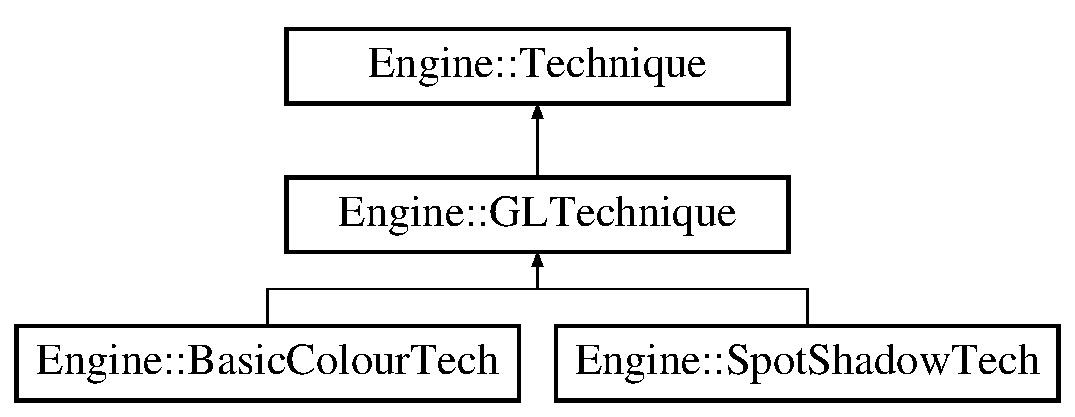
\includegraphics[height=3.000000cm]{classEngine_1_1GLTechnique}
\end{center}
\end{figure}
\subsection*{Public Member Functions}
\begin{DoxyCompactItemize}
\item 
\hypertarget{classEngine_1_1GLTechnique_a403e96effab192546279fe30079fb877}{}{\bfseries G\+L\+Technique} (const std\+::string \&name)\label{classEngine_1_1GLTechnique_a403e96effab192546279fe30079fb877}

\item 
\hypertarget{classEngine_1_1GLTechnique_aab149c687afdf57164ab1597e08e3ebd}{}void {\bfseries Render\+To\+Depth\+Texture\+Start} (\hyperlink{classEngine_1_1FrameBuffer}{Frame\+Buffer} $\ast$fbo, \hyperlink{classEngine_1_1OpenPolygonDisplay}{Open\+Polygon\+Display} $\ast$display)\label{classEngine_1_1GLTechnique_aab149c687afdf57164ab1597e08e3ebd}

\item 
\hypertarget{classEngine_1_1GLTechnique_afd809fd7e8b1bc4e09acd4201aff81f5}{}void {\bfseries Render\+To\+Depth\+Texture\+Stop} (\hyperlink{classEngine_1_1FrameBuffer}{Frame\+Buffer} $\ast$fbo)\label{classEngine_1_1GLTechnique_afd809fd7e8b1bc4e09acd4201aff81f5}

\item 
\hypertarget{classEngine_1_1GLTechnique_a219f5a080c241e893c52813e23ef2fd0}{}void {\bfseries Render\+To\+Basic\+Texture\+Start} (\hyperlink{classEngine_1_1FrameBuffer}{Frame\+Buffer} $\ast$fbo, \hyperlink{classEngine_1_1OpenPolygonDisplay}{Open\+Polygon\+Display} $\ast$display)\label{classEngine_1_1GLTechnique_a219f5a080c241e893c52813e23ef2fd0}

\item 
\hypertarget{classEngine_1_1GLTechnique_a9f68b1a23c48312fe50ea9be84d7b891}{}void {\bfseries Render\+To\+Basic\+Texture\+Stop} (\hyperlink{classEngine_1_1FrameBuffer}{Frame\+Buffer} $\ast$fbo)\label{classEngine_1_1GLTechnique_a9f68b1a23c48312fe50ea9be84d7b891}

\item 
\hypertarget{classEngine_1_1GLTechnique_afab4b07e70b837bc55acf97c3d09798a}{}void {\bfseries Render\+To\+Colour\+Texture\+Start} (\hyperlink{classEngine_1_1FrameBuffer}{Frame\+Buffer} $\ast$fbo, \hyperlink{classEngine_1_1OpenPolygonDisplay}{Open\+Polygon\+Display} $\ast$display, G\+Lenum buffers\mbox{[}$\,$\mbox{]})\label{classEngine_1_1GLTechnique_afab4b07e70b837bc55acf97c3d09798a}

\item 
\hypertarget{classEngine_1_1GLTechnique_a5c6be24fa37bfa63759c31c28f95c360}{}void {\bfseries Render\+To\+Colour\+Texture\+Stop} (\hyperlink{classEngine_1_1FrameBuffer}{Frame\+Buffer} $\ast$fbo)\label{classEngine_1_1GLTechnique_a5c6be24fa37bfa63759c31c28f95c360}

\end{DoxyCompactItemize}
\subsection*{Additional Inherited Members}


\subsection{Detailed Description}
The \hyperlink{classEngine_1_1GLTechnique}{G\+L\+Technique} -\/ abstract class. 

The documentation for this class was generated from the following files\+:\begin{DoxyCompactItemize}
\item 
include/\+Interface/G\+L\+Technique.\+h\item 
Engine/\+Technique/G\+L\+Technique.\+cpp\end{DoxyCompactItemize}

\hypertarget{classEngine_1_1GLTextureBuffer}{}\section{Engine\+:\+:G\+L\+Texture\+Buffer Class Reference}
\label{classEngine_1_1GLTextureBuffer}\index{Engine\+::\+G\+L\+Texture\+Buffer@{Engine\+::\+G\+L\+Texture\+Buffer}}


The \hyperlink{classEngine_1_1GLTextureBuffer}{G\+L\+Texture\+Buffer} class.  




{\ttfamily \#include $<$gltexturebuffer.\+h$>$}

Inheritance diagram for Engine\+:\+:G\+L\+Texture\+Buffer\+:\begin{figure}[H]
\begin{center}
\leavevmode
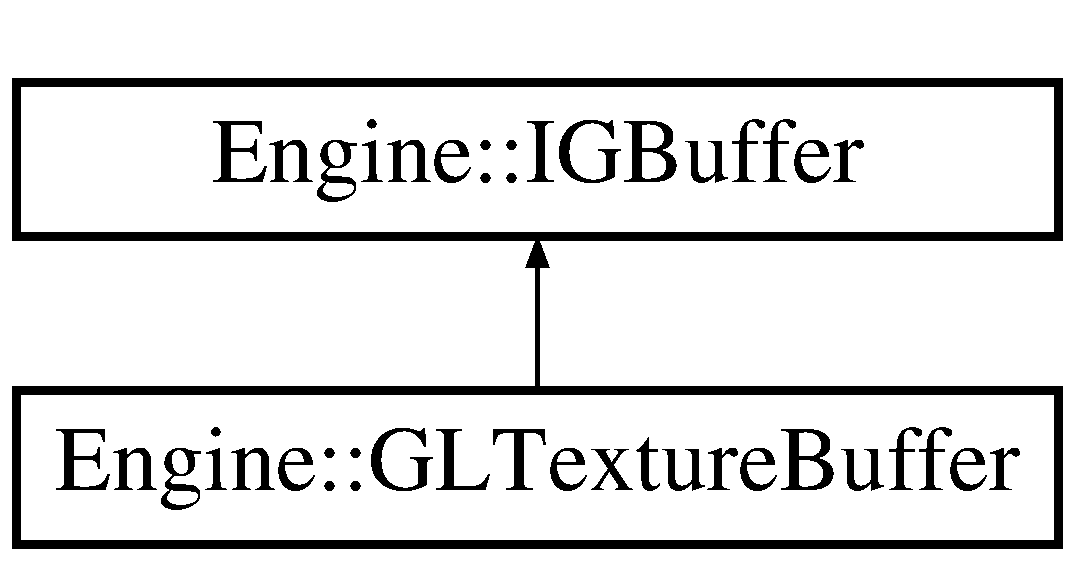
\includegraphics[height=2.000000cm]{classEngine_1_1GLTextureBuffer}
\end{center}
\end{figure}
\subsection*{Public Member Functions}
\begin{DoxyCompactItemize}
\item 
uint \hyperlink{classEngine_1_1GLTextureBuffer_aac493af54205e536a3ae7df812710f78}{create} (int size\+\_\+data, void $\ast$data)
\begin{DoxyCompactList}\small\item\em create \end{DoxyCompactList}\item 
void \hyperlink{classEngine_1_1GLTextureBuffer_a6b060dc1c33a9df000c011170daa46e2}{attach} (uint vao\+\_\+id)
\begin{DoxyCompactList}\small\item\em attach \end{DoxyCompactList}\item 
\hypertarget{classEngine_1_1GLTextureBuffer_abcda46bee777984efc9f6c485b6cb1ed}{}void {\bfseries update} (int offset, int size\+\_\+data, void $\ast$data)\label{classEngine_1_1GLTextureBuffer_abcda46bee777984efc9f6c485b6cb1ed}

\item 
void \hyperlink{classEngine_1_1GLTextureBuffer_a20a3044796531245f0c0926fdda52872}{get\+Data} (int offset, void $\ast$data)
\begin{DoxyCompactList}\small\item\em get\+Data \end{DoxyCompactList}\item 
void \hyperlink{classEngine_1_1GLTextureBuffer_ab64ccc1b8646be8d288b0781267fd909}{close} (void)
\begin{DoxyCompactList}\small\item\em close \end{DoxyCompactList}\end{DoxyCompactItemize}
\subsection*{Additional Inherited Members}


\subsection{Detailed Description}
The \hyperlink{classEngine_1_1GLTextureBuffer}{G\+L\+Texture\+Buffer} class. 

\subsection{Member Function Documentation}
\hypertarget{classEngine_1_1GLTextureBuffer_a6b060dc1c33a9df000c011170daa46e2}{}\index{Engine\+::\+G\+L\+Texture\+Buffer@{Engine\+::\+G\+L\+Texture\+Buffer}!attach@{attach}}
\index{attach@{attach}!Engine\+::\+G\+L\+Texture\+Buffer@{Engine\+::\+G\+L\+Texture\+Buffer}}
\subsubsection[{attach(uint vao\+\_\+id)}]{\setlength{\rightskip}{0pt plus 5cm}void G\+L\+Texture\+Buffer\+::attach (
\begin{DoxyParamCaption}
\item[{uint}]{vao\+\_\+id}
\end{DoxyParamCaption}
)\hspace{0.3cm}{\ttfamily [virtual]}}\label{classEngine_1_1GLTextureBuffer_a6b060dc1c33a9df000c011170daa46e2}


attach 


\begin{DoxyParams}{Parameters}
{\em vao\+\_\+id} & \\
\hline
\end{DoxyParams}


Implements \hyperlink{classEngine_1_1IGBuffer_a4d4186068930b5d161a52d2fa8afad02}{Engine\+::\+I\+G\+Buffer}.

\hypertarget{classEngine_1_1GLTextureBuffer_ab64ccc1b8646be8d288b0781267fd909}{}\index{Engine\+::\+G\+L\+Texture\+Buffer@{Engine\+::\+G\+L\+Texture\+Buffer}!close@{close}}
\index{close@{close}!Engine\+::\+G\+L\+Texture\+Buffer@{Engine\+::\+G\+L\+Texture\+Buffer}}
\subsubsection[{close(void)}]{\setlength{\rightskip}{0pt plus 5cm}void G\+L\+Texture\+Buffer\+::close (
\begin{DoxyParamCaption}
\item[{void}]{}
\end{DoxyParamCaption}
)\hspace{0.3cm}{\ttfamily [virtual]}}\label{classEngine_1_1GLTextureBuffer_ab64ccc1b8646be8d288b0781267fd909}


close 

Unbind G\+P\+U Buffer 

Implements \hyperlink{classEngine_1_1IGBuffer_a8473523f8cf850708f54859848f4234e}{Engine\+::\+I\+G\+Buffer}.

\hypertarget{classEngine_1_1GLTextureBuffer_aac493af54205e536a3ae7df812710f78}{}\index{Engine\+::\+G\+L\+Texture\+Buffer@{Engine\+::\+G\+L\+Texture\+Buffer}!create@{create}}
\index{create@{create}!Engine\+::\+G\+L\+Texture\+Buffer@{Engine\+::\+G\+L\+Texture\+Buffer}}
\subsubsection[{create(int size\+\_\+data, void $\ast$data)}]{\setlength{\rightskip}{0pt plus 5cm}uint G\+L\+Texture\+Buffer\+::create (
\begin{DoxyParamCaption}
\item[{int}]{size\+\_\+data, }
\item[{void $\ast$}]{data}
\end{DoxyParamCaption}
)\hspace{0.3cm}{\ttfamily [virtual]}}\label{classEngine_1_1GLTextureBuffer_aac493af54205e536a3ae7df812710f78}


create 

Create a new G\+P\+U Buffer 

Implements \hyperlink{classEngine_1_1IGBuffer_a6afbd1651d2c92fcec584e8d3ef1c32b}{Engine\+::\+I\+G\+Buffer}.

\hypertarget{classEngine_1_1GLTextureBuffer_a20a3044796531245f0c0926fdda52872}{}\index{Engine\+::\+G\+L\+Texture\+Buffer@{Engine\+::\+G\+L\+Texture\+Buffer}!get\+Data@{get\+Data}}
\index{get\+Data@{get\+Data}!Engine\+::\+G\+L\+Texture\+Buffer@{Engine\+::\+G\+L\+Texture\+Buffer}}
\subsubsection[{get\+Data(int offset, void $\ast$data)}]{\setlength{\rightskip}{0pt plus 5cm}void G\+L\+Texture\+Buffer\+::get\+Data (
\begin{DoxyParamCaption}
\item[{int}]{offset, }
\item[{void $\ast$}]{data}
\end{DoxyParamCaption}
)\hspace{0.3cm}{\ttfamily [virtual]}}\label{classEngine_1_1GLTextureBuffer_a20a3044796531245f0c0926fdda52872}


get\+Data 

Get Data from Buffer 
\begin{DoxyParams}{Parameters}
{\em offset} & \\
\hline
{\em size\+\_\+data} & \\
\hline
\end{DoxyParams}
\begin{DoxyReturn}{Returns}

\end{DoxyReturn}


Implements \hyperlink{classEngine_1_1IGBuffer_a8ad52dc670797d72aabf99033d20b220}{Engine\+::\+I\+G\+Buffer}.



The documentation for this class was generated from the following files\+:\begin{DoxyCompactItemize}
\item 
include/\+G\+P\+U/gltexturebuffer.\+h\item 
Engine/\+G\+P\+U/G\+L\+Texture\+Buffer.\+cpp\end{DoxyCompactItemize}

\hypertarget{classEngine_1_1GLVertexArrayObject}{}\section{Engine\+:\+:G\+L\+Vertex\+Array\+Object Class Reference}
\label{classEngine_1_1GLVertexArrayObject}\index{Engine\+::\+G\+L\+Vertex\+Array\+Object@{Engine\+::\+G\+L\+Vertex\+Array\+Object}}


The \hyperlink{classEngine_1_1GLVertexArrayObject}{G\+L\+Vertex\+Array\+Object} class.  




{\ttfamily \#include $<$glvertexarrayobject.\+h$>$}

\subsection*{Public Member Functions}
\begin{DoxyCompactItemize}
\item 
void \hyperlink{classEngine_1_1GLVertexArrayObject_ad2c7e334c24e3cbbb8450561e64ed32c}{set\+Draw\+Mode} (G\+Lenum draw\+\_\+mode)
\begin{DoxyCompactList}\small\item\em set\+Draw\+Mode \end{DoxyCompactList}\item 
void \hyperlink{classEngine_1_1GLVertexArrayObject_a5cb83f3cca36e9250c2ecd7747ee14c9}{create} (void)
\begin{DoxyCompactList}\small\item\em create \end{DoxyCompactList}\item 
void \hyperlink{classEngine_1_1GLVertexArrayObject_aa2fbd8bf27ddde48e6d6deab0a169a5f}{Bind} (void)
\begin{DoxyCompactList}\small\item\em Bind. \end{DoxyCompactList}\item 
void \hyperlink{classEngine_1_1GLVertexArrayObject_a2a64f18e180118d8b51ac30f8c9f6bf7}{Unbind} (void)
\begin{DoxyCompactList}\small\item\em Unbind. \end{DoxyCompactList}\item 
\hypertarget{classEngine_1_1GLVertexArrayObject_ac609320f7a23fbe91ad2d992c393a0eb}{}void {\bfseries Attach\+Buffer} (\hyperlink{classEngine_1_1GLVertexBuffer}{G\+L\+Vertex\+Buffer} $\ast$vbo\+\_\+vertex\+\_\+buffer)\label{classEngine_1_1GLVertexArrayObject_ac609320f7a23fbe91ad2d992c393a0eb}

\item 
\hypertarget{classEngine_1_1GLVertexArrayObject_a5b0c6bdbb98ce4c810e42427dd563754}{}void {\bfseries Attach\+Buffer} (\hyperlink{classEngine_1_1GLElementBuffer}{G\+L\+Element\+Buffer} $\ast$vbo\+\_\+element\+\_\+buffer)\label{classEngine_1_1GLVertexArrayObject_a5b0c6bdbb98ce4c810e42427dd563754}

\item 
\hypertarget{classEngine_1_1GLVertexArrayObject_aca1ce0b37547b8bd8b1ef2c4b30386b6}{}void {\bfseries Attach\+Buffer} (\hyperlink{structEngine_1_1AttributeCmd}{Attribute\+Cmd} \&cmd)\label{classEngine_1_1GLVertexArrayObject_aca1ce0b37547b8bd8b1ef2c4b30386b6}

\item 
\hypertarget{classEngine_1_1GLVertexArrayObject_a6080bc3aff814fc36d90bb13743d871b}{}void {\bfseries Attach\+Buffer} (uint attribute\+\_\+id, \hyperlink{classEngine_1_1IGBuffer}{I\+G\+Buffer} $\ast$vbo\+\_\+buffer)\label{classEngine_1_1GLVertexArrayObject_a6080bc3aff814fc36d90bb13743d871b}

\item 
\hypertarget{classEngine_1_1GLVertexArrayObject_a853c107480d1b74ef7f4fb04a54cb0d0}{}\hyperlink{classEngine_1_1IGBuffer}{I\+G\+Buffer} $\ast$ {\bfseries get\+Attach\+Buffer} (uint attribute\+\_\+id)\label{classEngine_1_1GLVertexArrayObject_a853c107480d1b74ef7f4fb04a54cb0d0}

\item 
\hypertarget{classEngine_1_1GLVertexArrayObject_a4cdfeb982fbc1461f40da899badc1375}{}void {\bfseries Draw\+Arrays} (void)\label{classEngine_1_1GLVertexArrayObject_a4cdfeb982fbc1461f40da899badc1375}

\item 
\hypertarget{classEngine_1_1GLVertexArrayObject_a14473fb252e4c84e06cb132d85a77c2e}{}void {\bfseries Draw\+Elements} (void)\label{classEngine_1_1GLVertexArrayObject_a14473fb252e4c84e06cb132d85a77c2e}

\item 
\hypertarget{classEngine_1_1GLVertexArrayObject_ab61900dca61790abfaebbcd43d8c8313}{}void {\bfseries Draw\+Elements\+Indirect} (int index\+\_\+size, int drawcount)\label{classEngine_1_1GLVertexArrayObject_ab61900dca61790abfaebbcd43d8c8313}

\item 
\hypertarget{classEngine_1_1GLVertexArrayObject_ade3dfd214cb75318e708abf2e86843a5}{}void {\bfseries Draw\+Elements\+Indirect} (int drawcount)\label{classEngine_1_1GLVertexArrayObject_ade3dfd214cb75318e708abf2e86843a5}

\item 
\hypertarget{classEngine_1_1GLVertexArrayObject_a4aa1b2050967f52bc0097898591b690c}{}void {\bfseries Draw\+Elements\+Instanced} (int drawcount)\label{classEngine_1_1GLVertexArrayObject_a4aa1b2050967f52bc0097898591b690c}

\end{DoxyCompactItemize}


\subsection{Detailed Description}
The \hyperlink{classEngine_1_1GLVertexArrayObject}{G\+L\+Vertex\+Array\+Object} class. 

\subsection{Member Function Documentation}
\hypertarget{classEngine_1_1GLVertexArrayObject_aa2fbd8bf27ddde48e6d6deab0a169a5f}{}\index{Engine\+::\+G\+L\+Vertex\+Array\+Object@{Engine\+::\+G\+L\+Vertex\+Array\+Object}!Bind@{Bind}}
\index{Bind@{Bind}!Engine\+::\+G\+L\+Vertex\+Array\+Object@{Engine\+::\+G\+L\+Vertex\+Array\+Object}}
\subsubsection[{Bind(void)}]{\setlength{\rightskip}{0pt plus 5cm}void G\+L\+Vertex\+Array\+Object\+::\+Bind (
\begin{DoxyParamCaption}
\item[{void}]{}
\end{DoxyParamCaption}
)}\label{classEngine_1_1GLVertexArrayObject_aa2fbd8bf27ddde48e6d6deab0a169a5f}


Bind. 

Use V\+A\+O I\+D Public \hypertarget{classEngine_1_1GLVertexArrayObject_a5cb83f3cca36e9250c2ecd7747ee14c9}{}\index{Engine\+::\+G\+L\+Vertex\+Array\+Object@{Engine\+::\+G\+L\+Vertex\+Array\+Object}!create@{create}}
\index{create@{create}!Engine\+::\+G\+L\+Vertex\+Array\+Object@{Engine\+::\+G\+L\+Vertex\+Array\+Object}}
\subsubsection[{create(void)}]{\setlength{\rightskip}{0pt plus 5cm}void G\+L\+Vertex\+Array\+Object\+::create (
\begin{DoxyParamCaption}
\item[{void}]{}
\end{DoxyParamCaption}
)}\label{classEngine_1_1GLVertexArrayObject_a5cb83f3cca36e9250c2ecd7747ee14c9}


create 

Create V\+A\+O I\+D \hypertarget{classEngine_1_1GLVertexArrayObject_ad2c7e334c24e3cbbb8450561e64ed32c}{}\index{Engine\+::\+G\+L\+Vertex\+Array\+Object@{Engine\+::\+G\+L\+Vertex\+Array\+Object}!set\+Draw\+Mode@{set\+Draw\+Mode}}
\index{set\+Draw\+Mode@{set\+Draw\+Mode}!Engine\+::\+G\+L\+Vertex\+Array\+Object@{Engine\+::\+G\+L\+Vertex\+Array\+Object}}
\subsubsection[{set\+Draw\+Mode(\+G\+Lenum draw\+\_\+mode)}]{\setlength{\rightskip}{0pt plus 5cm}void G\+L\+Vertex\+Array\+Object\+::set\+Draw\+Mode (
\begin{DoxyParamCaption}
\item[{G\+Lenum}]{draw\+\_\+mode}
\end{DoxyParamCaption}
)}\label{classEngine_1_1GLVertexArrayObject_ad2c7e334c24e3cbbb8450561e64ed32c}


set\+Draw\+Mode 

Draw\+Modes\+: G\+L\+\_\+\+T\+R\+I\+A\+N\+G\+L\+E\+S $\vert$ G\+L\+\_\+\+P\+O\+I\+N\+T\+S ... 
\begin{DoxyParams}{Parameters}
{\em draw\+\_\+mode} & \\
\hline
\end{DoxyParams}
\hypertarget{classEngine_1_1GLVertexArrayObject_a2a64f18e180118d8b51ac30f8c9f6bf7}{}\index{Engine\+::\+G\+L\+Vertex\+Array\+Object@{Engine\+::\+G\+L\+Vertex\+Array\+Object}!Unbind@{Unbind}}
\index{Unbind@{Unbind}!Engine\+::\+G\+L\+Vertex\+Array\+Object@{Engine\+::\+G\+L\+Vertex\+Array\+Object}}
\subsubsection[{Unbind(void)}]{\setlength{\rightskip}{0pt plus 5cm}void G\+L\+Vertex\+Array\+Object\+::\+Unbind (
\begin{DoxyParamCaption}
\item[{void}]{}
\end{DoxyParamCaption}
)}\label{classEngine_1_1GLVertexArrayObject_a2a64f18e180118d8b51ac30f8c9f6bf7}


Unbind. 

Use not V\+A\+O I\+D Public 

The documentation for this class was generated from the following files\+:\begin{DoxyCompactItemize}
\item 
include/\+G\+P\+U/glvertexarrayobject.\+h\item 
Engine/\+G\+P\+U/G\+L\+Vertex\+Array\+Object.\+cpp\end{DoxyCompactItemize}

\hypertarget{classEngine_1_1GLVertexBuffer}{}\section{Engine\+:\+:G\+L\+Vertex\+Buffer Class Reference}
\label{classEngine_1_1GLVertexBuffer}\index{Engine\+::\+G\+L\+Vertex\+Buffer@{Engine\+::\+G\+L\+Vertex\+Buffer}}


The \hyperlink{classEngine_1_1GLVertexBuffer}{G\+L\+Vertex\+Buffer} class.  




{\ttfamily \#include $<$glvertexbuffer.\+h$>$}

Inheritance diagram for Engine\+:\+:G\+L\+Vertex\+Buffer\+:\begin{figure}[H]
\begin{center}
\leavevmode
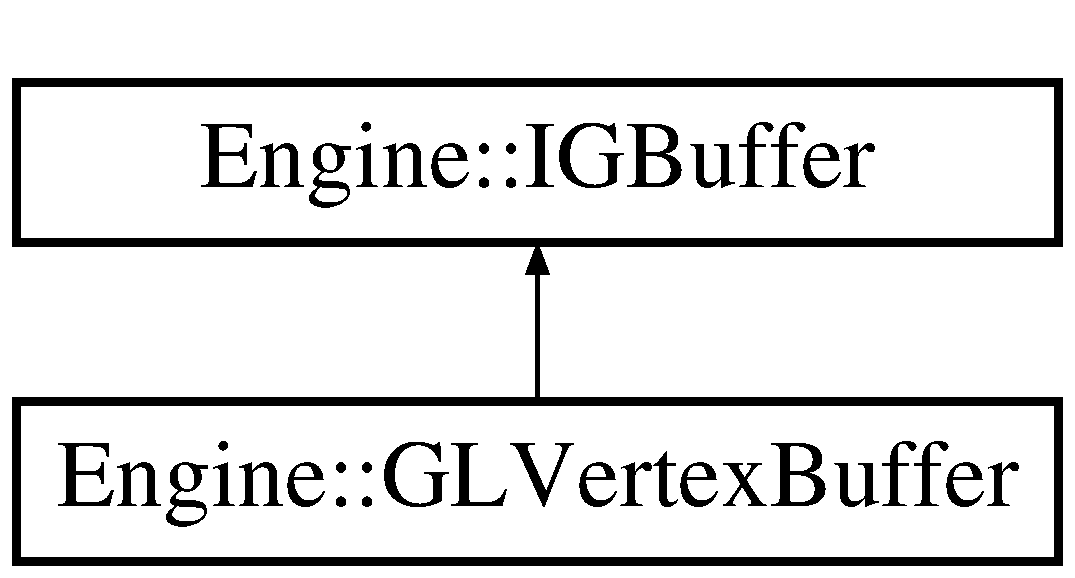
\includegraphics[height=2.000000cm]{classEngine_1_1GLVertexBuffer}
\end{center}
\end{figure}
\subsection*{Public Member Functions}
\begin{DoxyCompactItemize}
\item 
uint \hyperlink{classEngine_1_1GLVertexBuffer_a34314a2b1f249bec246508a39af02c66}{create} (int size\+\_\+data, void $\ast$data)
\begin{DoxyCompactList}\small\item\em create \end{DoxyCompactList}\item 
void \hyperlink{classEngine_1_1GLVertexBuffer_ae92c6c261902cbf1b7250ba559dec117}{attach} (uint vao\+\_\+id)
\begin{DoxyCompactList}\small\item\em attach \end{DoxyCompactList}\item 
\hypertarget{classEngine_1_1GLVertexBuffer_acdc9deee4ae75b09b84912303eb1a957}{}void {\bfseries update} (int offset, int size\+\_\+data, void $\ast$data)\label{classEngine_1_1GLVertexBuffer_acdc9deee4ae75b09b84912303eb1a957}

\item 
void \hyperlink{classEngine_1_1GLVertexBuffer_ad62200d5611e256f2f1df87d13bc9651}{get\+Data} (int offset, void $\ast$data)
\begin{DoxyCompactList}\small\item\em get\+Data \end{DoxyCompactList}\item 
void \hyperlink{classEngine_1_1GLVertexBuffer_a30af4a237541ae40c69983ceebf7363a}{close} (void)
\begin{DoxyCompactList}\small\item\em close \end{DoxyCompactList}\item 
\hypertarget{classEngine_1_1GLVertexBuffer_af1c126b18083ff76eaf0e9685ab45512}{}int {\bfseries get\+Float\+Count} (void)\label{classEngine_1_1GLVertexBuffer_af1c126b18083ff76eaf0e9685ab45512}

\item 
\hypertarget{classEngine_1_1GLVertexBuffer_a3592487858ab9b5c3b689af3765347fe}{}void {\bfseries set\+Float\+Count} (int amount)\label{classEngine_1_1GLVertexBuffer_a3592487858ab9b5c3b689af3765347fe}

\end{DoxyCompactItemize}
\subsection*{Additional Inherited Members}


\subsection{Detailed Description}
The \hyperlink{classEngine_1_1GLVertexBuffer}{G\+L\+Vertex\+Buffer} class. 

\subsection{Member Function Documentation}
\hypertarget{classEngine_1_1GLVertexBuffer_ae92c6c261902cbf1b7250ba559dec117}{}\index{Engine\+::\+G\+L\+Vertex\+Buffer@{Engine\+::\+G\+L\+Vertex\+Buffer}!attach@{attach}}
\index{attach@{attach}!Engine\+::\+G\+L\+Vertex\+Buffer@{Engine\+::\+G\+L\+Vertex\+Buffer}}
\subsubsection[{attach(uint vao\+\_\+id)}]{\setlength{\rightskip}{0pt plus 5cm}void G\+L\+Vertex\+Buffer\+::attach (
\begin{DoxyParamCaption}
\item[{uint}]{vao\+\_\+id}
\end{DoxyParamCaption}
)\hspace{0.3cm}{\ttfamily [virtual]}}\label{classEngine_1_1GLVertexBuffer_ae92c6c261902cbf1b7250ba559dec117}


attach 


\begin{DoxyParams}{Parameters}
{\em vao\+\_\+id} & \\
\hline
\end{DoxyParams}


Implements \hyperlink{classEngine_1_1IGBuffer_a4d4186068930b5d161a52d2fa8afad02}{Engine\+::\+I\+G\+Buffer}.

\hypertarget{classEngine_1_1GLVertexBuffer_a30af4a237541ae40c69983ceebf7363a}{}\index{Engine\+::\+G\+L\+Vertex\+Buffer@{Engine\+::\+G\+L\+Vertex\+Buffer}!close@{close}}
\index{close@{close}!Engine\+::\+G\+L\+Vertex\+Buffer@{Engine\+::\+G\+L\+Vertex\+Buffer}}
\subsubsection[{close(void)}]{\setlength{\rightskip}{0pt plus 5cm}void G\+L\+Vertex\+Buffer\+::close (
\begin{DoxyParamCaption}
\item[{void}]{}
\end{DoxyParamCaption}
)\hspace{0.3cm}{\ttfamily [virtual]}}\label{classEngine_1_1GLVertexBuffer_a30af4a237541ae40c69983ceebf7363a}


close 

Unbind G\+P\+U Buffer 

Implements \hyperlink{classEngine_1_1IGBuffer_a8473523f8cf850708f54859848f4234e}{Engine\+::\+I\+G\+Buffer}.

\hypertarget{classEngine_1_1GLVertexBuffer_a34314a2b1f249bec246508a39af02c66}{}\index{Engine\+::\+G\+L\+Vertex\+Buffer@{Engine\+::\+G\+L\+Vertex\+Buffer}!create@{create}}
\index{create@{create}!Engine\+::\+G\+L\+Vertex\+Buffer@{Engine\+::\+G\+L\+Vertex\+Buffer}}
\subsubsection[{create(int size\+\_\+data, void $\ast$data)}]{\setlength{\rightskip}{0pt plus 5cm}uint G\+L\+Vertex\+Buffer\+::create (
\begin{DoxyParamCaption}
\item[{int}]{size\+\_\+data, }
\item[{void $\ast$}]{data}
\end{DoxyParamCaption}
)\hspace{0.3cm}{\ttfamily [virtual]}}\label{classEngine_1_1GLVertexBuffer_a34314a2b1f249bec246508a39af02c66}


create 

Create a new G\+P\+U Buffer 

Implements \hyperlink{classEngine_1_1IGBuffer_a6afbd1651d2c92fcec584e8d3ef1c32b}{Engine\+::\+I\+G\+Buffer}.

\hypertarget{classEngine_1_1GLVertexBuffer_ad62200d5611e256f2f1df87d13bc9651}{}\index{Engine\+::\+G\+L\+Vertex\+Buffer@{Engine\+::\+G\+L\+Vertex\+Buffer}!get\+Data@{get\+Data}}
\index{get\+Data@{get\+Data}!Engine\+::\+G\+L\+Vertex\+Buffer@{Engine\+::\+G\+L\+Vertex\+Buffer}}
\subsubsection[{get\+Data(int offset, void $\ast$data)}]{\setlength{\rightskip}{0pt plus 5cm}void G\+L\+Vertex\+Buffer\+::get\+Data (
\begin{DoxyParamCaption}
\item[{int}]{offset, }
\item[{void $\ast$}]{data}
\end{DoxyParamCaption}
)\hspace{0.3cm}{\ttfamily [virtual]}}\label{classEngine_1_1GLVertexBuffer_ad62200d5611e256f2f1df87d13bc9651}


get\+Data 

Get Data from Buffer 
\begin{DoxyParams}{Parameters}
{\em offset} & \\
\hline
{\em size\+\_\+data} & \\
\hline
\end{DoxyParams}
\begin{DoxyReturn}{Returns}

\end{DoxyReturn}


Implements \hyperlink{classEngine_1_1IGBuffer_a8ad52dc670797d72aabf99033d20b220}{Engine\+::\+I\+G\+Buffer}.



The documentation for this class was generated from the following files\+:\begin{DoxyCompactItemize}
\item 
include/\+G\+P\+U/glvertexbuffer.\+h\item 
Engine/\+G\+P\+U/G\+L\+Vertex\+Buffer.\+cpp\end{DoxyCompactItemize}

\hypertarget{classEngine_1_1IComponent}{}\section{Engine\+:\+:I\+Component$<$ Sender $>$ Class Template Reference}
\label{classEngine_1_1IComponent}\index{Engine\+::\+I\+Component$<$ Sender $>$@{Engine\+::\+I\+Component$<$ Sender $>$}}


The \hyperlink{classEngine_1_1IComponent}{I\+Component} class.  




{\ttfamily \#include $<$I\+Component.\+h$>$}

\subsection*{Public Types}
\begin{DoxyCompactItemize}
\item 
using \hyperlink{classEngine_1_1IComponent_aade5c1f3aa7ac594acc104861fc761c4}{I\+Component\+List} = std\+::list$<$ \hyperlink{classEngine_1_1IComponent}{I\+Component}$<$ Sender $>$ $\ast$ $>$
\end{DoxyCompactItemize}
\subsection*{Public Member Functions}
\begin{DoxyCompactItemize}
\item 
\hyperlink{classEngine_1_1IComponent_a7b5acbdb4786c772e6c83735cf5a2ad6}{I\+Component} (const std\+::string \&component\+\_\+name)
\begin{DoxyCompactList}\small\item\em \hyperlink{classEngine_1_1IComponent}{I\+Component}. \end{DoxyCompactList}\item 
const std\+::string \& \hyperlink{classEngine_1_1IComponent_addee40bd0de98ebcf4566d8b95968e05}{get\+Name} (void) const 
\begin{DoxyCompactList}\small\item\em message \end{DoxyCompactList}\item 
uint \hyperlink{classEngine_1_1IComponent_af35ea9d64e2151e4641f73500ec8d19b}{get\+I\+D} (void) const 
\begin{DoxyCompactList}\small\item\em get\+I\+D \end{DoxyCompactList}\item 
void \hyperlink{classEngine_1_1IComponent_aad832773ebaaefc426394d7d5b3fb5e7}{add\+Component} (\hyperlink{classEngine_1_1IComponent}{I\+Component}$<$ Sender $>$ $\ast$component)
\begin{DoxyCompactList}\small\item\em add\+Component \end{DoxyCompactList}\item 
bool \hyperlink{classEngine_1_1IComponent_ab6ff658b9114391269ffa3d9f1d57e10}{has\+Component} (const std\+::string \&component\+\_\+name)
\begin{DoxyCompactList}\small\item\em has\+Component \end{DoxyCompactList}\item 
\hyperlink{classEngine_1_1IComponent}{I\+Component}$<$ Sender $>$ $\ast$ \hyperlink{classEngine_1_1IComponent_ac33863a371723db7aef928986ff942e1}{get\+Component} (const std\+::string \&component\+\_\+name)
\begin{DoxyCompactList}\small\item\em get\+Component \end{DoxyCompactList}\item 
\hyperlink{classEngine_1_1IComponent_aade5c1f3aa7ac594acc104861fc761c4}{I\+Component\+List} \hyperlink{classEngine_1_1IComponent_a30089eee0f95d222bed42c59e6615f05}{get\+Components} (const std\+::string \&component\+\_\+name)
\begin{DoxyCompactList}\small\item\em get\+Components \end{DoxyCompactList}\item 
void \hyperlink{classEngine_1_1IComponent_ae1ebe49fd115e2776a250ff11e94caf4}{remove} (\hyperlink{classEngine_1_1IComponent}{I\+Component}$<$ Sender $>$ $\ast$component)
\begin{DoxyCompactList}\small\item\em remove \end{DoxyCompactList}\end{DoxyCompactItemize}
\subsection*{Protected Attributes}
\begin{DoxyCompactItemize}
\item 
\hypertarget{classEngine_1_1IComponent_aec9a0ccb4f8e2df57615c2e26822cc43}{}uint {\bfseries m\+Component\+Id}\label{classEngine_1_1IComponent_aec9a0ccb4f8e2df57615c2e26822cc43}

\item 
\hypertarget{classEngine_1_1IComponent_a5eb3918b4b630214ba60af5d205c3515}{}\hyperlink{classEngine_1_1IComponent_aade5c1f3aa7ac594acc104861fc761c4}{I\+Component\+List} {\bfseries m\+Component\+List}\label{classEngine_1_1IComponent_a5eb3918b4b630214ba60af5d205c3515}

\end{DoxyCompactItemize}
\subsection*{Friends}
\begin{DoxyCompactItemize}
\item 
\hypertarget{classEngine_1_1IComponent_a4542618ef05fbb881e9783ae3755240a}{}class {\bfseries Component\+Manager}\label{classEngine_1_1IComponent_a4542618ef05fbb881e9783ae3755240a}

\end{DoxyCompactItemize}


\subsection{Detailed Description}
\subsubsection*{template$<$class Sender$>$class Engine\+::\+I\+Component$<$ Sender $>$}

The \hyperlink{classEngine_1_1IComponent}{I\+Component} class. 

Component Template Class 

\subsection{Member Typedef Documentation}
\hypertarget{classEngine_1_1IComponent_aade5c1f3aa7ac594acc104861fc761c4}{}\index{Engine\+::\+I\+Component@{Engine\+::\+I\+Component}!I\+Component\+List@{I\+Component\+List}}
\index{I\+Component\+List@{I\+Component\+List}!Engine\+::\+I\+Component@{Engine\+::\+I\+Component}}
\subsubsection[{I\+Component\+List}]{\setlength{\rightskip}{0pt plus 5cm}template$<$class Sender$>$ using {\bf Engine\+::\+I\+Component}$<$ Sender $>$\+::{\bf I\+Component\+List} =  std\+::list$<$ {\bf I\+Component}$<$Sender$>$ $\ast$ $>$}\label{classEngine_1_1IComponent_aade5c1f3aa7ac594acc104861fc761c4}
Component List 

\subsection{Constructor \& Destructor Documentation}
\hypertarget{classEngine_1_1IComponent_a7b5acbdb4786c772e6c83735cf5a2ad6}{}\index{Engine\+::\+I\+Component@{Engine\+::\+I\+Component}!I\+Component@{I\+Component}}
\index{I\+Component@{I\+Component}!Engine\+::\+I\+Component@{Engine\+::\+I\+Component}}
\subsubsection[{I\+Component(const std\+::string \&component\+\_\+name)}]{\setlength{\rightskip}{0pt plus 5cm}template$<$class Sender$>$ {\bf Engine\+::\+I\+Component}$<$ Sender $>$\+::{\bf I\+Component} (
\begin{DoxyParamCaption}
\item[{const std\+::string \&}]{component\+\_\+name}
\end{DoxyParamCaption}
)}\label{classEngine_1_1IComponent_a7b5acbdb4786c772e6c83735cf5a2ad6}


\hyperlink{classEngine_1_1IComponent}{I\+Component}. 

Default Constructor with Component Name 
\begin{DoxyParams}{Parameters}
{\em component\+\_\+name} & \\
\hline
\end{DoxyParams}


\subsection{Member Function Documentation}
\hypertarget{classEngine_1_1IComponent_aad832773ebaaefc426394d7d5b3fb5e7}{}\index{Engine\+::\+I\+Component@{Engine\+::\+I\+Component}!add\+Component@{add\+Component}}
\index{add\+Component@{add\+Component}!Engine\+::\+I\+Component@{Engine\+::\+I\+Component}}
\subsubsection[{add\+Component(\+I\+Component$<$ Sender $>$ $\ast$component)}]{\setlength{\rightskip}{0pt plus 5cm}template$<$class Sender $>$ void {\bf Engine\+::\+I\+Component}$<$ Sender $>$\+::add\+Component (
\begin{DoxyParamCaption}
\item[{{\bf I\+Component}$<$ Sender $>$ $\ast$}]{component}
\end{DoxyParamCaption}
)}\label{classEngine_1_1IComponent_aad832773ebaaefc426394d7d5b3fb5e7}


add\+Component 

Add Component 
\begin{DoxyParams}{Parameters}
{\em component} & \\
\hline
\end{DoxyParams}
\hypertarget{classEngine_1_1IComponent_ac33863a371723db7aef928986ff942e1}{}\index{Engine\+::\+I\+Component@{Engine\+::\+I\+Component}!get\+Component@{get\+Component}}
\index{get\+Component@{get\+Component}!Engine\+::\+I\+Component@{Engine\+::\+I\+Component}}
\subsubsection[{get\+Component(const std\+::string \&component\+\_\+name)}]{\setlength{\rightskip}{0pt plus 5cm}template$<$class Sender $>$ {\bf I\+Component}$<$ Sender $>$ $\ast$ {\bf Engine\+::\+I\+Component}$<$ Sender $>$\+::get\+Component (
\begin{DoxyParamCaption}
\item[{const std\+::string \&}]{component\+\_\+name}
\end{DoxyParamCaption}
)}\label{classEngine_1_1IComponent_ac33863a371723db7aef928986ff942e1}


get\+Component 

Return one Component by Component Name 
\begin{DoxyParams}{Parameters}
{\em component\+\_\+name} & \\
\hline
\end{DoxyParams}
\begin{DoxyReturn}{Returns}

\end{DoxyReturn}
\hypertarget{classEngine_1_1IComponent_a30089eee0f95d222bed42c59e6615f05}{}\index{Engine\+::\+I\+Component@{Engine\+::\+I\+Component}!get\+Components@{get\+Components}}
\index{get\+Components@{get\+Components}!Engine\+::\+I\+Component@{Engine\+::\+I\+Component}}
\subsubsection[{get\+Components(const std\+::string \&component\+\_\+name)}]{\setlength{\rightskip}{0pt plus 5cm}template$<$class Sender $>$ std\+::list$<$ {\bf I\+Component}$<$ Sender $>$ $\ast$ $>$ {\bf Engine\+::\+I\+Component}$<$ Sender $>$\+::get\+Components (
\begin{DoxyParamCaption}
\item[{const std\+::string \&}]{component\+\_\+name}
\end{DoxyParamCaption}
)}\label{classEngine_1_1IComponent_a30089eee0f95d222bed42c59e6615f05}


get\+Components 

Return more Component by Component Name 
\begin{DoxyParams}{Parameters}
{\em component\+\_\+name} & \\
\hline
\end{DoxyParams}
\begin{DoxyReturn}{Returns}

\end{DoxyReturn}
\hypertarget{classEngine_1_1IComponent_af35ea9d64e2151e4641f73500ec8d19b}{}\index{Engine\+::\+I\+Component@{Engine\+::\+I\+Component}!get\+I\+D@{get\+I\+D}}
\index{get\+I\+D@{get\+I\+D}!Engine\+::\+I\+Component@{Engine\+::\+I\+Component}}
\subsubsection[{get\+I\+D(void) const }]{\setlength{\rightskip}{0pt plus 5cm}template$<$class Sender $>$ uint {\bf Engine\+::\+I\+Component}$<$ Sender $>$\+::get\+I\+D (
\begin{DoxyParamCaption}
\item[{void}]{}
\end{DoxyParamCaption}
) const}\label{classEngine_1_1IComponent_af35ea9d64e2151e4641f73500ec8d19b}


get\+I\+D 

Return Component I\+D \begin{DoxyReturn}{Returns}

\end{DoxyReturn}
\hypertarget{classEngine_1_1IComponent_addee40bd0de98ebcf4566d8b95968e05}{}\index{Engine\+::\+I\+Component@{Engine\+::\+I\+Component}!get\+Name@{get\+Name}}
\index{get\+Name@{get\+Name}!Engine\+::\+I\+Component@{Engine\+::\+I\+Component}}
\subsubsection[{get\+Name(void) const }]{\setlength{\rightskip}{0pt plus 5cm}template$<$class Sender $>$ const std\+::string \& {\bf Engine\+::\+I\+Component}$<$ Sender $>$\+::get\+Name (
\begin{DoxyParamCaption}
\item[{void}]{}
\end{DoxyParamCaption}
) const}\label{classEngine_1_1IComponent_addee40bd0de98ebcf4566d8b95968e05}


message 

Received a Message from another Sender ( aka. Component ) 
\begin{DoxyParams}{Parameters}
{\em sender} & \\
\hline
{\em msg} & \\
\hline
\end{DoxyParams}
\begin{DoxyReturn}{Returns}

\end{DoxyReturn}
Return Component Name get\+Name \begin{DoxyReturn}{Returns}

\end{DoxyReturn}
\hypertarget{classEngine_1_1IComponent_ab6ff658b9114391269ffa3d9f1d57e10}{}\index{Engine\+::\+I\+Component@{Engine\+::\+I\+Component}!has\+Component@{has\+Component}}
\index{has\+Component@{has\+Component}!Engine\+::\+I\+Component@{Engine\+::\+I\+Component}}
\subsubsection[{has\+Component(const std\+::string \&component\+\_\+name)}]{\setlength{\rightskip}{0pt plus 5cm}template$<$class Sender $>$ bool {\bf Engine\+::\+I\+Component}$<$ Sender $>$\+::has\+Component (
\begin{DoxyParamCaption}
\item[{const std\+::string \&}]{component\+\_\+name}
\end{DoxyParamCaption}
)}\label{classEngine_1_1IComponent_ab6ff658b9114391269ffa3d9f1d57e10}


has\+Component 

Return true if component exists 
\begin{DoxyParams}{Parameters}
{\em component\+\_\+name} & \\
\hline
\end{DoxyParams}
\begin{DoxyReturn}{Returns}

\end{DoxyReturn}
\hypertarget{classEngine_1_1IComponent_ae1ebe49fd115e2776a250ff11e94caf4}{}\index{Engine\+::\+I\+Component@{Engine\+::\+I\+Component}!remove@{remove}}
\index{remove@{remove}!Engine\+::\+I\+Component@{Engine\+::\+I\+Component}}
\subsubsection[{remove(\+I\+Component$<$ Sender $>$ $\ast$component)}]{\setlength{\rightskip}{0pt plus 5cm}template$<$class Sender $>$ void {\bf Engine\+::\+I\+Component}$<$ Sender $>$\+::remove (
\begin{DoxyParamCaption}
\item[{{\bf I\+Component}$<$ Sender $>$ $\ast$}]{component}
\end{DoxyParamCaption}
)}\label{classEngine_1_1IComponent_ae1ebe49fd115e2776a250ff11e94caf4}


remove 

Destroy one any Component 
\begin{DoxyParams}{Parameters}
{\em component} & \\
\hline
\end{DoxyParams}


The documentation for this class was generated from the following file\+:\begin{DoxyCompactItemize}
\item 
include/I\+Component.\+h\end{DoxyCompactItemize}

\hypertarget{classEngine_1_1IGBuffer}{}\section{Engine\+:\+:I\+G\+Buffer Class Reference}
\label{classEngine_1_1IGBuffer}\index{Engine\+::\+I\+G\+Buffer@{Engine\+::\+I\+G\+Buffer}}


The \hyperlink{classEngine_1_1IGBuffer}{I\+G\+Buffer} -\/ Interface class.  




{\ttfamily \#include $<$I\+G\+Buffer.\+h$>$}

Inheritance diagram for Engine\+:\+:I\+G\+Buffer\+:\begin{figure}[H]
\begin{center}
\leavevmode
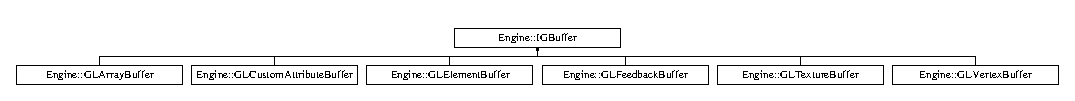
\includegraphics[height=0.915033cm]{classEngine_1_1IGBuffer}
\end{center}
\end{figure}
\subsection*{Public Member Functions}
\begin{DoxyCompactItemize}
\item 
virtual uint \hyperlink{classEngine_1_1IGBuffer_a6afbd1651d2c92fcec584e8d3ef1c32b}{create} (int size\+\_\+data, void $\ast$data)=0
\begin{DoxyCompactList}\small\item\em create \end{DoxyCompactList}\item 
virtual void \hyperlink{classEngine_1_1IGBuffer_a4d4186068930b5d161a52d2fa8afad02}{attach} (uint vao\+\_\+id)=0
\begin{DoxyCompactList}\small\item\em attach \end{DoxyCompactList}\item 
\hypertarget{classEngine_1_1IGBuffer_a84ea7b6d09875a37b6ac9adb7aab6c30}{}virtual void {\bfseries update} (int offset, int size\+\_\+data, void $\ast$data)=0\label{classEngine_1_1IGBuffer_a84ea7b6d09875a37b6ac9adb7aab6c30}

\item 
virtual void \hyperlink{classEngine_1_1IGBuffer_a8ad52dc670797d72aabf99033d20b220}{get\+Data} (int offset, void $\ast$data)=0
\begin{DoxyCompactList}\small\item\em get\+Data \end{DoxyCompactList}\item 
virtual void \hyperlink{classEngine_1_1IGBuffer_a8473523f8cf850708f54859848f4234e}{close} (void)=0
\begin{DoxyCompactList}\small\item\em close \end{DoxyCompactList}\end{DoxyCompactItemize}
\subsection*{Protected Attributes}
\begin{DoxyCompactItemize}
\item 
\hypertarget{classEngine_1_1IGBuffer_a17938a3956a10f9e01a287a9fe7ac15d}{}uint {\bfseries m\+\_\+vbo\+\_\+buffer\+\_\+id}\label{classEngine_1_1IGBuffer_a17938a3956a10f9e01a287a9fe7ac15d}

\item 
\hypertarget{classEngine_1_1IGBuffer_a037d8a933c32d1feec60e84fc818a861}{}int {\bfseries m\+\_\+size\+\_\+data}\label{classEngine_1_1IGBuffer_a037d8a933c32d1feec60e84fc818a861}

\end{DoxyCompactItemize}


\subsection{Detailed Description}
The \hyperlink{classEngine_1_1IGBuffer}{I\+G\+Buffer} -\/ Interface class. 

\subsection{Member Function Documentation}
\hypertarget{classEngine_1_1IGBuffer_a4d4186068930b5d161a52d2fa8afad02}{}\index{Engine\+::\+I\+G\+Buffer@{Engine\+::\+I\+G\+Buffer}!attach@{attach}}
\index{attach@{attach}!Engine\+::\+I\+G\+Buffer@{Engine\+::\+I\+G\+Buffer}}
\subsubsection[{attach(uint vao\+\_\+id)=0}]{\setlength{\rightskip}{0pt plus 5cm}virtual void Engine\+::\+I\+G\+Buffer\+::attach (
\begin{DoxyParamCaption}
\item[{uint}]{vao\+\_\+id}
\end{DoxyParamCaption}
)\hspace{0.3cm}{\ttfamily [pure virtual]}}\label{classEngine_1_1IGBuffer_a4d4186068930b5d161a52d2fa8afad02}


attach 


\begin{DoxyParams}{Parameters}
{\em vao\+\_\+id} & \\
\hline
\end{DoxyParams}


Implemented in \hyperlink{classEngine_1_1GLCustomAttributeBuffer_a0decec64cba335e28acd81268650c3b3}{Engine\+::\+G\+L\+Custom\+Attribute\+Buffer}, \hyperlink{classEngine_1_1GLFeedbackBuffer_ae1d18bd14a843d4fcd030998498128c6}{Engine\+::\+G\+L\+Feedback\+Buffer}, \hyperlink{classEngine_1_1GLTextureBuffer_a6b060dc1c33a9df000c011170daa46e2}{Engine\+::\+G\+L\+Texture\+Buffer}, \hyperlink{classEngine_1_1GLVertexBuffer_ae92c6c261902cbf1b7250ba559dec117}{Engine\+::\+G\+L\+Vertex\+Buffer}, \hyperlink{classEngine_1_1GLArrayBuffer_a5c31588067f1f10c0c9f35aedd8b73af}{Engine\+::\+G\+L\+Array\+Buffer}, and \hyperlink{classEngine_1_1GLElementBuffer_a12e74567261194e53b9b58b52ff91da4}{Engine\+::\+G\+L\+Element\+Buffer}.

\hypertarget{classEngine_1_1IGBuffer_a8473523f8cf850708f54859848f4234e}{}\index{Engine\+::\+I\+G\+Buffer@{Engine\+::\+I\+G\+Buffer}!close@{close}}
\index{close@{close}!Engine\+::\+I\+G\+Buffer@{Engine\+::\+I\+G\+Buffer}}
\subsubsection[{close(void)=0}]{\setlength{\rightskip}{0pt plus 5cm}virtual void Engine\+::\+I\+G\+Buffer\+::close (
\begin{DoxyParamCaption}
\item[{void}]{}
\end{DoxyParamCaption}
)\hspace{0.3cm}{\ttfamily [pure virtual]}}\label{classEngine_1_1IGBuffer_a8473523f8cf850708f54859848f4234e}


close 

Unbind G\+P\+U Buffer 

Implemented in \hyperlink{classEngine_1_1GLCustomAttributeBuffer_a84dd56904b35cd71f6a8866c36063f5d}{Engine\+::\+G\+L\+Custom\+Attribute\+Buffer}, \hyperlink{classEngine_1_1GLFeedbackBuffer_a278dd1fdb1b2fe62a30b7711ea1090a2}{Engine\+::\+G\+L\+Feedback\+Buffer}, \hyperlink{classEngine_1_1GLTextureBuffer_ab64ccc1b8646be8d288b0781267fd909}{Engine\+::\+G\+L\+Texture\+Buffer}, \hyperlink{classEngine_1_1GLVertexBuffer_a30af4a237541ae40c69983ceebf7363a}{Engine\+::\+G\+L\+Vertex\+Buffer}, \hyperlink{classEngine_1_1GLArrayBuffer_aa6e0bd973444f5c23bf94fdc88e2e5ca}{Engine\+::\+G\+L\+Array\+Buffer}, and \hyperlink{classEngine_1_1GLElementBuffer_a8d46099a8a43d1ac1217e765863997ea}{Engine\+::\+G\+L\+Element\+Buffer}.

\hypertarget{classEngine_1_1IGBuffer_a6afbd1651d2c92fcec584e8d3ef1c32b}{}\index{Engine\+::\+I\+G\+Buffer@{Engine\+::\+I\+G\+Buffer}!create@{create}}
\index{create@{create}!Engine\+::\+I\+G\+Buffer@{Engine\+::\+I\+G\+Buffer}}
\subsubsection[{create(int size\+\_\+data, void $\ast$data)=0}]{\setlength{\rightskip}{0pt plus 5cm}virtual uint Engine\+::\+I\+G\+Buffer\+::create (
\begin{DoxyParamCaption}
\item[{int}]{size\+\_\+data, }
\item[{void $\ast$}]{data}
\end{DoxyParamCaption}
)\hspace{0.3cm}{\ttfamily [pure virtual]}}\label{classEngine_1_1IGBuffer_a6afbd1651d2c92fcec584e8d3ef1c32b}


create 

Create a new G\+P\+U Buffer 

Implemented in \hyperlink{classEngine_1_1GLCustomAttributeBuffer_a41743693090a4ea7d0021f61d80e83a8}{Engine\+::\+G\+L\+Custom\+Attribute\+Buffer}, \hyperlink{classEngine_1_1GLFeedbackBuffer_af07b1ef217ec8a8c77412fe417564428}{Engine\+::\+G\+L\+Feedback\+Buffer}, \hyperlink{classEngine_1_1GLTextureBuffer_aac493af54205e536a3ae7df812710f78}{Engine\+::\+G\+L\+Texture\+Buffer}, \hyperlink{classEngine_1_1GLVertexBuffer_a34314a2b1f249bec246508a39af02c66}{Engine\+::\+G\+L\+Vertex\+Buffer}, \hyperlink{classEngine_1_1GLArrayBuffer_aec618c4096d7b6d2ab39dde5fb55976b}{Engine\+::\+G\+L\+Array\+Buffer}, and \hyperlink{classEngine_1_1GLElementBuffer_a36ddf0be23d19af69b60b0a1502768c5}{Engine\+::\+G\+L\+Element\+Buffer}.

\hypertarget{classEngine_1_1IGBuffer_a8ad52dc670797d72aabf99033d20b220}{}\index{Engine\+::\+I\+G\+Buffer@{Engine\+::\+I\+G\+Buffer}!get\+Data@{get\+Data}}
\index{get\+Data@{get\+Data}!Engine\+::\+I\+G\+Buffer@{Engine\+::\+I\+G\+Buffer}}
\subsubsection[{get\+Data(int offset, void $\ast$data)=0}]{\setlength{\rightskip}{0pt plus 5cm}virtual void Engine\+::\+I\+G\+Buffer\+::get\+Data (
\begin{DoxyParamCaption}
\item[{int}]{offset, }
\item[{void $\ast$}]{data}
\end{DoxyParamCaption}
)\hspace{0.3cm}{\ttfamily [pure virtual]}}\label{classEngine_1_1IGBuffer_a8ad52dc670797d72aabf99033d20b220}


get\+Data 

Get Data from Buffer 
\begin{DoxyParams}{Parameters}
{\em offset} & \\
\hline
{\em size\+\_\+data} & \\
\hline
\end{DoxyParams}
\begin{DoxyReturn}{Returns}

\end{DoxyReturn}


Implemented in \hyperlink{classEngine_1_1GLCustomAttributeBuffer_a828a015ce58e25c6422505f0cadfd799}{Engine\+::\+G\+L\+Custom\+Attribute\+Buffer}, \hyperlink{classEngine_1_1GLFeedbackBuffer_a8c4b82243c6652f377d7511ade32e7b5}{Engine\+::\+G\+L\+Feedback\+Buffer}, \hyperlink{classEngine_1_1GLTextureBuffer_a20a3044796531245f0c0926fdda52872}{Engine\+::\+G\+L\+Texture\+Buffer}, \hyperlink{classEngine_1_1GLVertexBuffer_ad62200d5611e256f2f1df87d13bc9651}{Engine\+::\+G\+L\+Vertex\+Buffer}, \hyperlink{classEngine_1_1GLArrayBuffer_a6ca4905a31d11d291df25abbfe95f177}{Engine\+::\+G\+L\+Array\+Buffer}, and \hyperlink{classEngine_1_1GLElementBuffer_a78842b1b2910f198665096b72186a1be}{Engine\+::\+G\+L\+Element\+Buffer}.



The documentation for this class was generated from the following file\+:\begin{DoxyCompactItemize}
\item 
include/\+Interface/I\+G\+Buffer.\+h\end{DoxyCompactItemize}

\hypertarget{classEngine_1_1IGDoubleBuffer}{}\section{Engine\+:\+:I\+G\+Double\+Buffer Class Reference}
\label{classEngine_1_1IGDoubleBuffer}\index{Engine\+::\+I\+G\+Double\+Buffer@{Engine\+::\+I\+G\+Double\+Buffer}}


The \hyperlink{classEngine_1_1IGDoubleBuffer}{I\+G\+Double\+Buffer} -\/ abstract / interface class.  




{\ttfamily \#include $<$I\+G\+Double\+Buffer.\+h$>$}

Inheritance diagram for Engine\+:\+:I\+G\+Double\+Buffer\+:\begin{figure}[H]
\begin{center}
\leavevmode
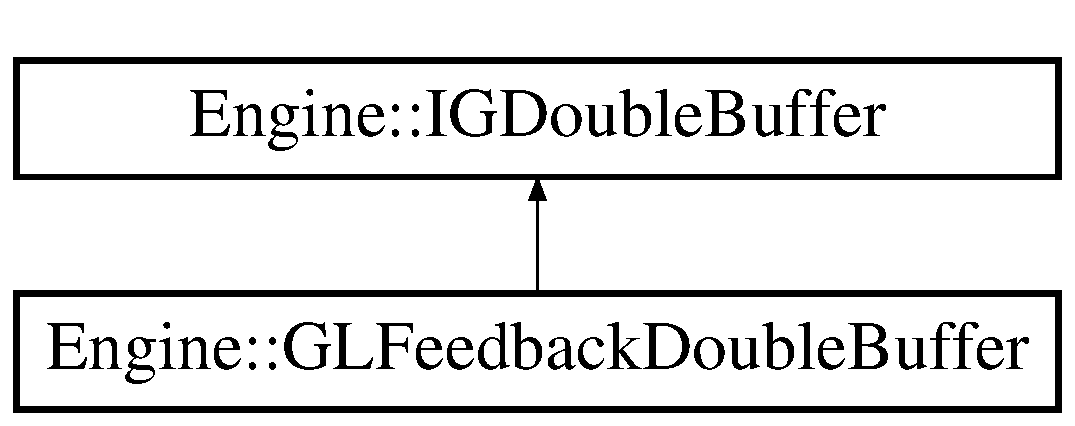
\includegraphics[height=2.000000cm]{classEngine_1_1IGDoubleBuffer}
\end{center}
\end{figure}
\subsection*{Public Member Functions}
\begin{DoxyCompactItemize}
\item 
virtual void \hyperlink{classEngine_1_1IGDoubleBuffer_a094e87543bb24956ec1fd3835b4ca413}{create} (\hyperlink{classEngine_1_1IGBuffer}{I\+G\+Buffer} $\ast$front, \hyperlink{classEngine_1_1IGBuffer}{I\+G\+Buffer} $\ast$back, int size\+\_\+data)=0
\begin{DoxyCompactList}\small\item\em create \end{DoxyCompactList}\item 
virtual void \hyperlink{classEngine_1_1IGDoubleBuffer_a39b0608ee6f5ddbf14dbea9030b881d8}{update} (int offset, int size\+\_\+data, void $\ast$data)=0
\begin{DoxyCompactList}\small\item\em update \end{DoxyCompactList}\item 
virtual void \hyperlink{classEngine_1_1IGDoubleBuffer_ade7c5ce0b5883c55f5e66588dd8b14da}{Swap\+Buffers} (void)=0
\begin{DoxyCompactList}\small\item\em Swap\+Buffers. \end{DoxyCompactList}\item 
\hypertarget{classEngine_1_1IGDoubleBuffer_aceed4fb6fb4c4a2d1250ded26a28efd2}{}uint {\bfseries get\+Front\+Buffer\+I\+D} (void)\label{classEngine_1_1IGDoubleBuffer_aceed4fb6fb4c4a2d1250ded26a28efd2}

\item 
\hypertarget{classEngine_1_1IGDoubleBuffer_a724bc8379533fb5b245fd32447188d03}{}uint {\bfseries get\+Back\+Buffer\+I\+D} (void)\label{classEngine_1_1IGDoubleBuffer_a724bc8379533fb5b245fd32447188d03}

\end{DoxyCompactItemize}
\subsection*{Protected Attributes}
\begin{DoxyCompactItemize}
\item 
\hypertarget{classEngine_1_1IGDoubleBuffer_a092ac82c99c506737a6c8dc6908d89c2}{}uint {\bfseries m\+\_\+front\+\_\+buffer\+\_\+id}\label{classEngine_1_1IGDoubleBuffer_a092ac82c99c506737a6c8dc6908d89c2}

\item 
\hypertarget{classEngine_1_1IGDoubleBuffer_a658ad8de4c92a70b57ecb0c8d6517121}{}uint {\bfseries m\+\_\+back\+\_\+buffer\+\_\+id}\label{classEngine_1_1IGDoubleBuffer_a658ad8de4c92a70b57ecb0c8d6517121}

\item 
\hypertarget{classEngine_1_1IGDoubleBuffer_a42e859171e27646ace0e000a8a26ac16}{}int {\bfseries m\+\_\+size\+\_\+data}\label{classEngine_1_1IGDoubleBuffer_a42e859171e27646ace0e000a8a26ac16}

\end{DoxyCompactItemize}


\subsection{Detailed Description}
The \hyperlink{classEngine_1_1IGDoubleBuffer}{I\+G\+Double\+Buffer} -\/ abstract / interface class. 

\subsection{Member Function Documentation}
\hypertarget{classEngine_1_1IGDoubleBuffer_a094e87543bb24956ec1fd3835b4ca413}{}\index{Engine\+::\+I\+G\+Double\+Buffer@{Engine\+::\+I\+G\+Double\+Buffer}!create@{create}}
\index{create@{create}!Engine\+::\+I\+G\+Double\+Buffer@{Engine\+::\+I\+G\+Double\+Buffer}}
\subsubsection[{create(\+I\+G\+Buffer $\ast$front, I\+G\+Buffer $\ast$back, int size\+\_\+data)=0}]{\setlength{\rightskip}{0pt plus 5cm}virtual void Engine\+::\+I\+G\+Double\+Buffer\+::create (
\begin{DoxyParamCaption}
\item[{{\bf I\+G\+Buffer} $\ast$}]{front, }
\item[{{\bf I\+G\+Buffer} $\ast$}]{back, }
\item[{int}]{size\+\_\+data}
\end{DoxyParamCaption}
)\hspace{0.3cm}{\ttfamily [pure virtual]}}\label{classEngine_1_1IGDoubleBuffer_a094e87543bb24956ec1fd3835b4ca413}


create 

Create Front and Back Buffer 

Implemented in \hyperlink{classEngine_1_1GLFeedbackDoubleBuffer_a093faa032cd6f229c6a0e6b18fca11b6}{Engine\+::\+G\+L\+Feedback\+Double\+Buffer}.

\hypertarget{classEngine_1_1IGDoubleBuffer_ade7c5ce0b5883c55f5e66588dd8b14da}{}\index{Engine\+::\+I\+G\+Double\+Buffer@{Engine\+::\+I\+G\+Double\+Buffer}!Swap\+Buffers@{Swap\+Buffers}}
\index{Swap\+Buffers@{Swap\+Buffers}!Engine\+::\+I\+G\+Double\+Buffer@{Engine\+::\+I\+G\+Double\+Buffer}}
\subsubsection[{Swap\+Buffers(void)=0}]{\setlength{\rightskip}{0pt plus 5cm}virtual void Engine\+::\+I\+G\+Double\+Buffer\+::\+Swap\+Buffers (
\begin{DoxyParamCaption}
\item[{void}]{}
\end{DoxyParamCaption}
)\hspace{0.3cm}{\ttfamily [pure virtual]}}\label{classEngine_1_1IGDoubleBuffer_ade7c5ce0b5883c55f5e66588dd8b14da}


Swap\+Buffers. 

Copy Back Buffer into Front Buffer 

Implemented in \hyperlink{classEngine_1_1GLFeedbackDoubleBuffer_aee224416eeeaa26f4c1eb0158cde1f68}{Engine\+::\+G\+L\+Feedback\+Double\+Buffer}.

\hypertarget{classEngine_1_1IGDoubleBuffer_a39b0608ee6f5ddbf14dbea9030b881d8}{}\index{Engine\+::\+I\+G\+Double\+Buffer@{Engine\+::\+I\+G\+Double\+Buffer}!update@{update}}
\index{update@{update}!Engine\+::\+I\+G\+Double\+Buffer@{Engine\+::\+I\+G\+Double\+Buffer}}
\subsubsection[{update(int offset, int size\+\_\+data, void $\ast$data)=0}]{\setlength{\rightskip}{0pt plus 5cm}virtual void Engine\+::\+I\+G\+Double\+Buffer\+::update (
\begin{DoxyParamCaption}
\item[{int}]{offset, }
\item[{int}]{size\+\_\+data, }
\item[{void $\ast$}]{data}
\end{DoxyParamCaption}
)\hspace{0.3cm}{\ttfamily [pure virtual]}}\label{classEngine_1_1IGDoubleBuffer_a39b0608ee6f5ddbf14dbea9030b881d8}


update 

Update Back Buffer 
\begin{DoxyParams}{Parameters}
{\em size\+\_\+data} & \\
\hline
{\em data} & \\
\hline
\end{DoxyParams}


Implemented in \hyperlink{classEngine_1_1GLFeedbackDoubleBuffer_a94805048c8b23cb2bf83d40ace22c9cd}{Engine\+::\+G\+L\+Feedback\+Double\+Buffer}.



The documentation for this class was generated from the following file\+:\begin{DoxyCompactItemize}
\item 
include/\+Interface/I\+G\+Double\+Buffer.\+h\end{DoxyCompactItemize}

\hypertarget{classEngine_1_1InputListener}{}\section{Engine\+:\+:Input\+Listener Class Reference}
\label{classEngine_1_1InputListener}\index{Engine\+::\+Input\+Listener@{Engine\+::\+Input\+Listener}}


The \hyperlink{classEngine_1_1InputListener}{Input\+Listener} -\/ Interface class.  




{\ttfamily \#include $<$input.\+h$>$}

Inheritance diagram for Engine\+:\+:Input\+Listener\+:\begin{figure}[H]
\begin{center}
\leavevmode
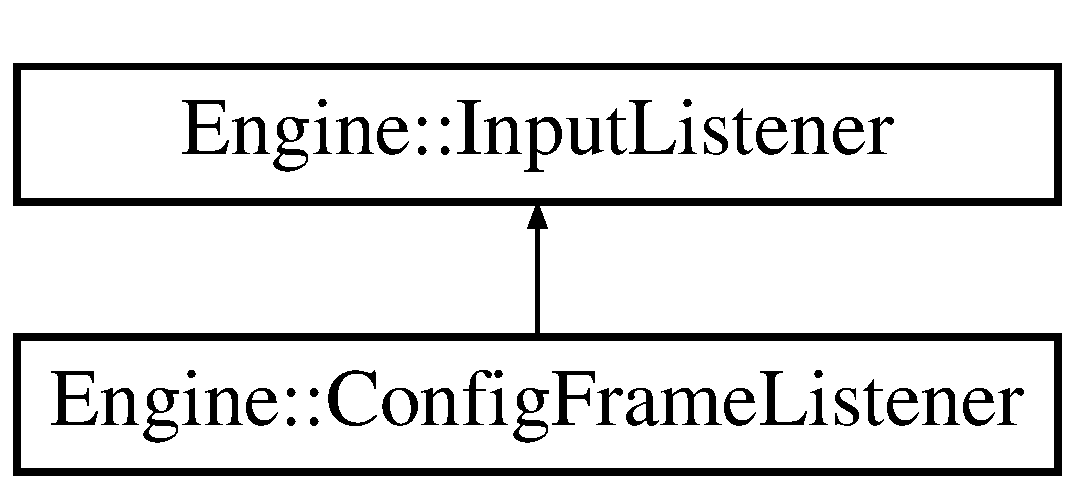
\includegraphics[height=2.000000cm]{classEngine_1_1InputListener}
\end{center}
\end{figure}
\subsection*{Public Member Functions}
\begin{DoxyCompactItemize}
\item 
virtual void \hyperlink{classEngine_1_1InputListener_abcd5e74a03230108bf29f68f74c1a878}{on\+Key\+Event} (const \hyperlink{classEngine_1_1KeyEvent}{Key\+Event} \&event)=0
\begin{DoxyCompactList}\small\item\em on\+Key\+Event \end{DoxyCompactList}\item 
virtual void \hyperlink{classEngine_1_1InputListener_aeee4d9f56950838b71d17ece61656736}{on\+Mouse\+Event} (const \hyperlink{classEngine_1_1MouseEvent}{Mouse\+Event} \&event)=0
\begin{DoxyCompactList}\small\item\em on\+Mouse\+Event \end{DoxyCompactList}\end{DoxyCompactItemize}


\subsection{Detailed Description}
The \hyperlink{classEngine_1_1InputListener}{Input\+Listener} -\/ Interface class. 

\subsection{Member Function Documentation}
\hypertarget{classEngine_1_1InputListener_abcd5e74a03230108bf29f68f74c1a878}{}\index{Engine\+::\+Input\+Listener@{Engine\+::\+Input\+Listener}!on\+Key\+Event@{on\+Key\+Event}}
\index{on\+Key\+Event@{on\+Key\+Event}!Engine\+::\+Input\+Listener@{Engine\+::\+Input\+Listener}}
\subsubsection[{on\+Key\+Event(const Key\+Event \&event)=0}]{\setlength{\rightskip}{0pt plus 5cm}virtual void Engine\+::\+Input\+Listener\+::on\+Key\+Event (
\begin{DoxyParamCaption}
\item[{const {\bf Key\+Event} \&}]{event}
\end{DoxyParamCaption}
)\hspace{0.3cm}{\ttfamily [pure virtual]}}\label{classEngine_1_1InputListener_abcd5e74a03230108bf29f68f74c1a878}


on\+Key\+Event 

Catch a Keyboard Event 
\begin{DoxyParams}{Parameters}
{\em event} & \\
\hline
\end{DoxyParams}


Implemented in \hyperlink{classEngine_1_1ConfigFrameListener_a2e412a7541868de93953c7cd818a6968}{Engine\+::\+Config\+Frame\+Listener}.

\hypertarget{classEngine_1_1InputListener_aeee4d9f56950838b71d17ece61656736}{}\index{Engine\+::\+Input\+Listener@{Engine\+::\+Input\+Listener}!on\+Mouse\+Event@{on\+Mouse\+Event}}
\index{on\+Mouse\+Event@{on\+Mouse\+Event}!Engine\+::\+Input\+Listener@{Engine\+::\+Input\+Listener}}
\subsubsection[{on\+Mouse\+Event(const Mouse\+Event \&event)=0}]{\setlength{\rightskip}{0pt plus 5cm}virtual void Engine\+::\+Input\+Listener\+::on\+Mouse\+Event (
\begin{DoxyParamCaption}
\item[{const {\bf Mouse\+Event} \&}]{event}
\end{DoxyParamCaption}
)\hspace{0.3cm}{\ttfamily [pure virtual]}}\label{classEngine_1_1InputListener_aeee4d9f56950838b71d17ece61656736}


on\+Mouse\+Event 

Catch a Mouse Event 
\begin{DoxyParams}{Parameters}
{\em event} & \\
\hline
\end{DoxyParams}


Implemented in \hyperlink{classEngine_1_1ConfigFrameListener_ac293a2b4c841a19e39d5e3d74eeb6ec3}{Engine\+::\+Config\+Frame\+Listener}.



The documentation for this class was generated from the following file\+:\begin{DoxyCompactItemize}
\item 
include/\+Container/input.\+h\end{DoxyCompactItemize}

\hypertarget{classEngine_1_1InputManager}{}\section{Engine\+:\+:Input\+Manager Class Reference}
\label{classEngine_1_1InputManager}\index{Engine\+::\+Input\+Manager@{Engine\+::\+Input\+Manager}}


The \hyperlink{classEngine_1_1InputManager}{Input\+Manager} controlled \hyperlink{classEngine_1_1InputListener}{Input\+Listener}.  




{\ttfamily \#include $<$input.\+h$>$}

\subsection*{Public Member Functions}
\begin{DoxyCompactItemize}
\item 
\hypertarget{classEngine_1_1InputManager_aad9dc1be66eb9e4aa297f05d6f52796f}{}void {\bfseries Poll\+Events} (G\+L\+F\+Wwindow $\ast$window)\label{classEngine_1_1InputManager_aad9dc1be66eb9e4aa297f05d6f52796f}

\item 
void \hyperlink{classEngine_1_1InputManager_a2173a6568e83a87457dea29d6a2cbcfa}{add\+Input\+Listener} (\hyperlink{classEngine_1_1InputListener}{Input\+Listener} $\ast$listener)
\begin{DoxyCompactList}\small\item\em add\+Input\+Listener \end{DoxyCompactList}\item 
void \hyperlink{classEngine_1_1InputManager_afa38a27cafb58cdaf0b961b62a4ccb5a}{remove\+Listener} (\hyperlink{classEngine_1_1InputListener}{Input\+Listener} $\ast$listener)
\begin{DoxyCompactList}\small\item\em remove\+Listener \end{DoxyCompactList}\item 
void \hyperlink{classEngine_1_1InputManager_a831f77f0da50898510e384b6551c7526}{capture} (int mouse\+X, int mouse\+Y)
\begin{DoxyCompactList}\small\item\em capture \end{DoxyCompactList}\item 
void \hyperlink{classEngine_1_1InputManager_a519d703bd33f1bb168e758f7938279dd}{create\+Key\+Board\+Event} (int key, int scancode, int action, int mods)
\begin{DoxyCompactList}\small\item\em create\+Key\+Board\+Event \end{DoxyCompactList}\item 
\hypertarget{classEngine_1_1InputManager_aa58b9b680a69eac6c3fd26ef6a480110}{}void {\bfseries create\+Key\+List\+Event} (std\+::list$<$ int $>$ keys)\label{classEngine_1_1InputManager_aa58b9b680a69eac6c3fd26ef6a480110}

\item 
void \hyperlink{classEngine_1_1InputManager_a62aab81c0b4c43dad82ad84feb32487c}{create\+Mouse\+Event} (int button, int action, int mods)
\begin{DoxyCompactList}\small\item\em create\+Mouse\+Event \end{DoxyCompactList}\item 
\hyperlink{classVector2}{Vector2f} \& \hyperlink{classEngine_1_1InputManager_a398d43ff9c84e95767523ca74de12ed9}{get\+Mouse\+Position} (void)
\begin{DoxyCompactList}\small\item\em get\+Mouse\+Position \end{DoxyCompactList}\item 
I\+Listener\+List \& \hyperlink{classEngine_1_1InputManager_a34f49a2a02ab0f7d44ee404978836711}{get\+Listener} ()
\begin{DoxyCompactList}\small\item\em get\+Listener \end{DoxyCompactList}\end{DoxyCompactItemize}
\subsection*{Static Public Member Functions}
\begin{DoxyCompactItemize}
\item 
static \hyperlink{classEngine_1_1InputManager}{Input\+Manager} $\ast$ \hyperlink{classEngine_1_1InputManager_a2cdade9d1d20018f8ad556b5a571beda}{get\+Singleton\+Ptr} (void)
\begin{DoxyCompactList}\small\item\em get\+Singleton\+Ptr \end{DoxyCompactList}\end{DoxyCompactItemize}


\subsection{Detailed Description}
The \hyperlink{classEngine_1_1InputManager}{Input\+Manager} controlled \hyperlink{classEngine_1_1InputListener}{Input\+Listener}. 

Management of Input Devices


\begin{DoxyItemize}
\item create Keyboard Event
\item create Mouse Event 
\end{DoxyItemize}

\subsection{Member Function Documentation}
\hypertarget{classEngine_1_1InputManager_a2173a6568e83a87457dea29d6a2cbcfa}{}\index{Engine\+::\+Input\+Manager@{Engine\+::\+Input\+Manager}!add\+Input\+Listener@{add\+Input\+Listener}}
\index{add\+Input\+Listener@{add\+Input\+Listener}!Engine\+::\+Input\+Manager@{Engine\+::\+Input\+Manager}}
\subsubsection[{add\+Input\+Listener(\+Input\+Listener $\ast$listener)}]{\setlength{\rightskip}{0pt plus 5cm}void Input\+Manager\+::add\+Input\+Listener (
\begin{DoxyParamCaption}
\item[{{\bf Input\+Listener} $\ast$}]{listener}
\end{DoxyParamCaption}
)}\label{classEngine_1_1InputManager_a2173a6568e83a87457dea29d6a2cbcfa}


add\+Input\+Listener 

Add Input Listener 
\begin{DoxyParams}{Parameters}
{\em listener} & \\
\hline
\end{DoxyParams}
\hypertarget{classEngine_1_1InputManager_a831f77f0da50898510e384b6551c7526}{}\index{Engine\+::\+Input\+Manager@{Engine\+::\+Input\+Manager}!capture@{capture}}
\index{capture@{capture}!Engine\+::\+Input\+Manager@{Engine\+::\+Input\+Manager}}
\subsubsection[{capture(int mouse\+X, int mouse\+Y)}]{\setlength{\rightskip}{0pt plus 5cm}void Input\+Manager\+::capture (
\begin{DoxyParamCaption}
\item[{int}]{mouse\+X, }
\item[{int}]{mouse\+Y}
\end{DoxyParamCaption}
)}\label{classEngine_1_1InputManager_a831f77f0da50898510e384b6551c7526}


capture 

Capture Mouse and Save x,y data 
\begin{DoxyParams}{Parameters}
{\em mouse\+X} & \\
\hline
{\em mouse\+Y} & \\
\hline
\end{DoxyParams}
\hypertarget{classEngine_1_1InputManager_a519d703bd33f1bb168e758f7938279dd}{}\index{Engine\+::\+Input\+Manager@{Engine\+::\+Input\+Manager}!create\+Key\+Board\+Event@{create\+Key\+Board\+Event}}
\index{create\+Key\+Board\+Event@{create\+Key\+Board\+Event}!Engine\+::\+Input\+Manager@{Engine\+::\+Input\+Manager}}
\subsubsection[{create\+Key\+Board\+Event(int key, int scancode, int action, int mods)}]{\setlength{\rightskip}{0pt plus 5cm}void Input\+Manager\+::create\+Key\+Board\+Event (
\begin{DoxyParamCaption}
\item[{int}]{key, }
\item[{int}]{scancode, }
\item[{int}]{action, }
\item[{int}]{mods}
\end{DoxyParamCaption}
)}\label{classEngine_1_1InputManager_a519d703bd33f1bb168e758f7938279dd}


create\+Key\+Board\+Event 

Create a Keyboard Event 
\begin{DoxyParams}{Parameters}
{\em key} & \\
\hline
{\em scancode} & \\
\hline
{\em action} & \\
\hline
{\em mods} & \\
\hline
\end{DoxyParams}
\hypertarget{classEngine_1_1InputManager_a62aab81c0b4c43dad82ad84feb32487c}{}\index{Engine\+::\+Input\+Manager@{Engine\+::\+Input\+Manager}!create\+Mouse\+Event@{create\+Mouse\+Event}}
\index{create\+Mouse\+Event@{create\+Mouse\+Event}!Engine\+::\+Input\+Manager@{Engine\+::\+Input\+Manager}}
\subsubsection[{create\+Mouse\+Event(int button, int action, int mods)}]{\setlength{\rightskip}{0pt plus 5cm}void Input\+Manager\+::create\+Mouse\+Event (
\begin{DoxyParamCaption}
\item[{int}]{button, }
\item[{int}]{action, }
\item[{int}]{mods}
\end{DoxyParamCaption}
)}\label{classEngine_1_1InputManager_a62aab81c0b4c43dad82ad84feb32487c}


create\+Mouse\+Event 

Create a Mouse Event 
\begin{DoxyParams}{Parameters}
{\em button} & \\
\hline
{\em action} & \\
\hline
{\em mods} & \\
\hline
\end{DoxyParams}
\hypertarget{classEngine_1_1InputManager_a34f49a2a02ab0f7d44ee404978836711}{}\index{Engine\+::\+Input\+Manager@{Engine\+::\+Input\+Manager}!get\+Listener@{get\+Listener}}
\index{get\+Listener@{get\+Listener}!Engine\+::\+Input\+Manager@{Engine\+::\+Input\+Manager}}
\subsubsection[{get\+Listener()}]{\setlength{\rightskip}{0pt plus 5cm}I\+Listener\+List \& Input\+Manager\+::get\+Listener (
\begin{DoxyParamCaption}
\item[{void}]{}
\end{DoxyParamCaption}
)}\label{classEngine_1_1InputManager_a34f49a2a02ab0f7d44ee404978836711}


get\+Listener 

Return all Listener \begin{DoxyReturn}{Returns}

\end{DoxyReturn}
\hypertarget{classEngine_1_1InputManager_a398d43ff9c84e95767523ca74de12ed9}{}\index{Engine\+::\+Input\+Manager@{Engine\+::\+Input\+Manager}!get\+Mouse\+Position@{get\+Mouse\+Position}}
\index{get\+Mouse\+Position@{get\+Mouse\+Position}!Engine\+::\+Input\+Manager@{Engine\+::\+Input\+Manager}}
\subsubsection[{get\+Mouse\+Position(void)}]{\setlength{\rightskip}{0pt plus 5cm}{\bf Vector2f} \& Input\+Manager\+::get\+Mouse\+Position (
\begin{DoxyParamCaption}
\item[{void}]{}
\end{DoxyParamCaption}
)}\label{classEngine_1_1InputManager_a398d43ff9c84e95767523ca74de12ed9}


get\+Mouse\+Position 

Return Mouse \hyperlink{classEngine_1_1Position}{Position} \begin{DoxyReturn}{Returns}

\end{DoxyReturn}
\hypertarget{classEngine_1_1InputManager_a2cdade9d1d20018f8ad556b5a571beda}{}\index{Engine\+::\+Input\+Manager@{Engine\+::\+Input\+Manager}!get\+Singleton\+Ptr@{get\+Singleton\+Ptr}}
\index{get\+Singleton\+Ptr@{get\+Singleton\+Ptr}!Engine\+::\+Input\+Manager@{Engine\+::\+Input\+Manager}}
\subsubsection[{get\+Singleton\+Ptr(void)}]{\setlength{\rightskip}{0pt plus 5cm}{\bf Input\+Manager} $\ast$ Input\+Manager\+::get\+Singleton\+Ptr (
\begin{DoxyParamCaption}
\item[{void}]{}
\end{DoxyParamCaption}
)\hspace{0.3cm}{\ttfamily [static]}}\label{classEngine_1_1InputManager_a2cdade9d1d20018f8ad556b5a571beda}


get\+Singleton\+Ptr 

Return \hyperlink{classEngine_1_1InputManager}{Input\+Manager} Instance \begin{DoxyReturn}{Returns}

\end{DoxyReturn}
\hypertarget{classEngine_1_1InputManager_afa38a27cafb58cdaf0b961b62a4ccb5a}{}\index{Engine\+::\+Input\+Manager@{Engine\+::\+Input\+Manager}!remove\+Listener@{remove\+Listener}}
\index{remove\+Listener@{remove\+Listener}!Engine\+::\+Input\+Manager@{Engine\+::\+Input\+Manager}}
\subsubsection[{remove\+Listener(\+Input\+Listener $\ast$listener)}]{\setlength{\rightskip}{0pt plus 5cm}void Input\+Manager\+::remove\+Listener (
\begin{DoxyParamCaption}
\item[{{\bf Input\+Listener} $\ast$}]{listener}
\end{DoxyParamCaption}
)}\label{classEngine_1_1InputManager_afa38a27cafb58cdaf0b961b62a4ccb5a}


remove\+Listener 

Remove Input Listener 
\begin{DoxyParams}{Parameters}
{\em listener} & \\
\hline
\end{DoxyParams}


The documentation for this class was generated from the following files\+:\begin{DoxyCompactItemize}
\item 
include/\+Container/input.\+h\item 
Engine/\+Manager/Input\+Manager.\+cpp\end{DoxyCompactItemize}

\hypertarget{classEngine_1_1InstanceConfig}{}\section{Engine\+:\+:Instance\+Config$<$ In\+Config $>$ Class Template Reference}
\label{classEngine_1_1InstanceConfig}\index{Engine\+::\+Instance\+Config$<$ In\+Config $>$@{Engine\+::\+Instance\+Config$<$ In\+Config $>$}}
\subsection*{Public Member Functions}
\begin{DoxyCompactItemize}
\item 
\hypertarget{classEngine_1_1InstanceConfig_a2adcdc7358ffd19d08fe804d0f61a3b6}{}{\bfseries Instance\+Config} (const std\+::string \&file\+\_\+name)\label{classEngine_1_1InstanceConfig_a2adcdc7358ffd19d08fe804d0f61a3b6}

\item 
\hypertarget{classEngine_1_1InstanceConfig_a3a93c829611478c03b8e97a1cf173e13}{}void {\bfseries load} (void)\label{classEngine_1_1InstanceConfig_a3a93c829611478c03b8e97a1cf173e13}

\item 
\hypertarget{classEngine_1_1InstanceConfig_ad5de551d2a4f49abce419a5d6cb01129}{}void {\bfseries add\+Function} (const std\+::string \&value, \hyperlink{structEngine_1_1Callback}{Callback}$<$ In\+Config $>$ $\ast$callback)\label{classEngine_1_1InstanceConfig_ad5de551d2a4f49abce419a5d6cb01129}

\item 
\hypertarget{classEngine_1_1InstanceConfig_a4fee466021ff7a615d3863e2c6df97d3}{}struct \hyperlink{structEngine_1_1Callback}{Callback}$<$ In\+Config $>$ $\ast$ {\bfseries callback} (In\+Config $\ast$object, void(In\+Config\+::$\ast$callback)(const std\+::string \&file\+\_\+line\+\_\+input))\label{classEngine_1_1InstanceConfig_a4fee466021ff7a615d3863e2c6df97d3}

\item 
\hypertarget{classEngine_1_1InstanceConfig_a71c7847307e003c480597abf1780a39b}{}void {\bfseries free} (void)\label{classEngine_1_1InstanceConfig_a71c7847307e003c480597abf1780a39b}

\end{DoxyCompactItemize}
\subsection*{Protected Attributes}
\begin{DoxyCompactItemize}
\item 
\hypertarget{classEngine_1_1InstanceConfig_a9c7136fc6b9f955295137eb1fcaaaf27}{}std\+::string {\bfseries m\+File\+Name}\label{classEngine_1_1InstanceConfig_a9c7136fc6b9f955295137eb1fcaaaf27}

\item 
\hypertarget{classEngine_1_1InstanceConfig_af82c9ec4b58e0edbef1ecba1f7eb9e14}{}In\+Config\+Map {\bfseries m\+Config\+Map}\label{classEngine_1_1InstanceConfig_af82c9ec4b58e0edbef1ecba1f7eb9e14}

\end{DoxyCompactItemize}
\subsection*{Friends}
\begin{DoxyCompactItemize}
\item 
\hypertarget{classEngine_1_1InstanceConfig_aed8714396345e5fc5b1a2bf7ccaed500}{}class {\bfseries Config\+Manager}\label{classEngine_1_1InstanceConfig_aed8714396345e5fc5b1a2bf7ccaed500}

\end{DoxyCompactItemize}


The documentation for this class was generated from the following file\+:\begin{DoxyCompactItemize}
\item 
include/\+Manager/configmanager.\+h\end{DoxyCompactItemize}

\hypertarget{classEngine_1_1IShader}{}\section{Engine\+:\+:I\+Shader Class Reference}
\label{classEngine_1_1IShader}\index{Engine\+::\+I\+Shader@{Engine\+::\+I\+Shader}}


The \hyperlink{classEngine_1_1IShader}{I\+Shader} -\/ abstract / interface class.  




{\ttfamily \#include $<$I\+Shader.\+h$>$}

Inheritance diagram for Engine\+:\+:I\+Shader\+:\begin{figure}[H]
\begin{center}
\leavevmode
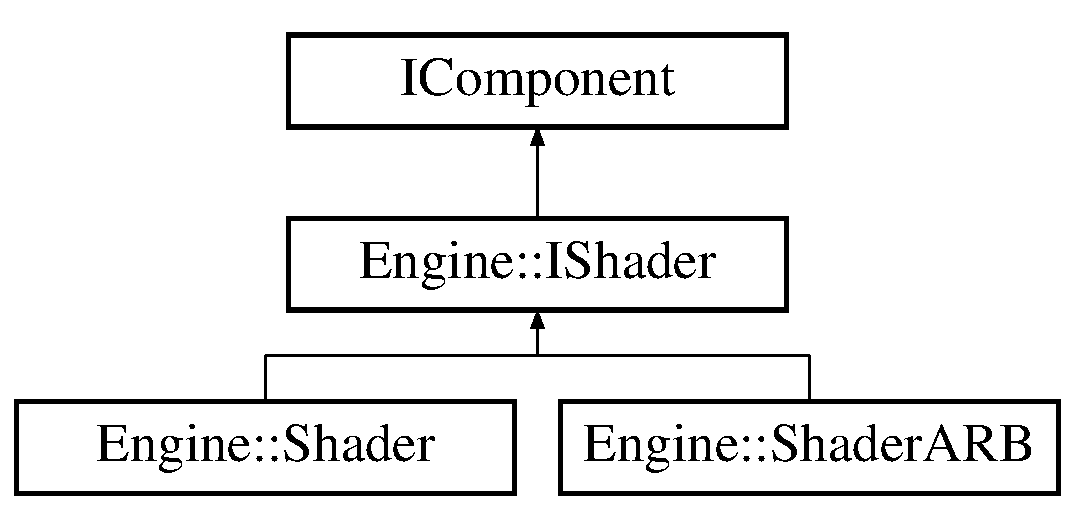
\includegraphics[height=3.000000cm]{classEngine_1_1IShader}
\end{center}
\end{figure}
\subsection*{Public Member Functions}
\begin{DoxyCompactItemize}
\item 
\hypertarget{classEngine_1_1IShader_a5b790df387d044b86556bcc9f61953ea}{}virtual void {\bfseries Use\+Program} (void)=0\label{classEngine_1_1IShader_a5b790df387d044b86556bcc9f61953ea}

\item 
\hypertarget{classEngine_1_1IShader_a979b8b793e0431d5f25421778c8f8fcf}{}virtual void {\bfseries Unused} (void)=0\label{classEngine_1_1IShader_a979b8b793e0431d5f25421778c8f8fcf}

\item 
\hypertarget{classEngine_1_1IShader_a40cd920be17e3bb211f22ee3c71560f6}{}virtual void {\bfseries Link\+Program} (void)=0\label{classEngine_1_1IShader_a40cd920be17e3bb211f22ee3c71560f6}

\item 
\hypertarget{classEngine_1_1IShader_a36e24542bc551a7ce2d5d60f7c23e304}{}virtual void {\bfseries Attach\+Shader} (uint shader)=0\label{classEngine_1_1IShader_a36e24542bc551a7ce2d5d60f7c23e304}

\item 
\hypertarget{classEngine_1_1IShader_a8999bac5bb0d4dc4a0a4e950be9b1262}{}virtual void {\bfseries Bind\+Uniform1i} (const char $\ast$location, int number)=0\label{classEngine_1_1IShader_a8999bac5bb0d4dc4a0a4e950be9b1262}

\item 
\hypertarget{classEngine_1_1IShader_a6b5824382ab0c62691c9b656b09d105d}{}virtual void {\bfseries Bind\+Uniform1f} (const char $\ast$location, float number)=0\label{classEngine_1_1IShader_a6b5824382ab0c62691c9b656b09d105d}

\item 
\hypertarget{classEngine_1_1IShader_aab732a9285162e51cb06bc722af5aa61}{}virtual void {\bfseries Bind\+Matrix} (const char $\ast$location, glm\+::mat4 matrix)=0\label{classEngine_1_1IShader_aab732a9285162e51cb06bc722af5aa61}

\item 
\hypertarget{classEngine_1_1IShader_aa61545153ee0887922e41de4d884a238}{}virtual void {\bfseries Bind\+Vec3i} (const char $\ast$location, const \hyperlink{classVector3}{Vector3i} \&vector)=0\label{classEngine_1_1IShader_aa61545153ee0887922e41de4d884a238}

\item 
\hypertarget{classEngine_1_1IShader_a14a8cadb90c6fc388151696ac1ebeddc}{}virtual void {\bfseries Bind\+Vec3f} (const char $\ast$location, const \hyperlink{classVector3}{Vector3f} \&vector)=0\label{classEngine_1_1IShader_a14a8cadb90c6fc388151696ac1ebeddc}

\item 
\hypertarget{classEngine_1_1IShader_ae89d7b6e3645ec29de4aca13e5e1f804}{}virtual void {\bfseries Bind\+Vec4i} (const char $\ast$location, const \hyperlink{classVector4}{Vector4i} \&vector)=0\label{classEngine_1_1IShader_ae89d7b6e3645ec29de4aca13e5e1f804}

\item 
\hypertarget{classEngine_1_1IShader_a8ce7543b1ba4bc008656fd74fecdfef2}{}virtual void {\bfseries Bind\+Vec4f} (const char $\ast$location, const \hyperlink{classVector4}{Vector4f} \&vector)=0\label{classEngine_1_1IShader_a8ce7543b1ba4bc008656fd74fecdfef2}

\item 
\hypertarget{classEngine_1_1IShader_a907a1a7a4b8c5c8b77e624a8bee5d478}{}virtual void {\bfseries Bind\+Texture} (\hyperlink{classEngine_1_1Texture}{Texture} $\ast$texture, const char $\ast$location, int texture\+\_\+unit)=0\label{classEngine_1_1IShader_a907a1a7a4b8c5c8b77e624a8bee5d478}

\item 
\hypertarget{classEngine_1_1IShader_a5af3bbe28c3347215fc23b95bb7700d8}{}virtual void {\bfseries Bind\+Frag\+Data} (const char $\ast$location, int frag\+\_\+position)=0\label{classEngine_1_1IShader_a5af3bbe28c3347215fc23b95bb7700d8}

\item 
\hypertarget{classEngine_1_1IShader_a3130202482a59d635328874b3b2b0d27}{}virtual void {\bfseries Bind\+Attribute\+Location} (const char $\ast$location, int attribute\+\_\+id)=0\label{classEngine_1_1IShader_a3130202482a59d635328874b3b2b0d27}

\item 
\hypertarget{classEngine_1_1IShader_a062e75d0707ff374417c3fe93c12168d}{}bool {\bfseries is\+Using} (void)\label{classEngine_1_1IShader_a062e75d0707ff374417c3fe93c12168d}

\item 
\hypertarget{classEngine_1_1IShader_a763243affdfa7f8b2aa90ecb37f40819}{}void {\bfseries set\+Using} (bool state)\label{classEngine_1_1IShader_a763243affdfa7f8b2aa90ecb37f40819}

\item 
\hypertarget{classEngine_1_1IShader_a0cff6b110c3b1d5788da38d006cd1043}{}void {\bfseries set\+Linked} (bool state)\label{classEngine_1_1IShader_a0cff6b110c3b1d5788da38d006cd1043}

\item 
\hypertarget{classEngine_1_1IShader_ab736c917289026225631c7c8bcc2b48b}{}void {\bfseries set\+Source} (bool state)\label{classEngine_1_1IShader_ab736c917289026225631c7c8bcc2b48b}

\item 
\hypertarget{classEngine_1_1IShader_afc547c25eed06f96e5a23be6bc3936bd}{}uint {\bfseries get\+Program} (void)\label{classEngine_1_1IShader_afc547c25eed06f96e5a23be6bc3936bd}

\item 
\hypertarget{classEngine_1_1IShader_a9bdb56da0500f9fd59992a2387c42a0f}{}bool {\bfseries has\+Source} (void)\label{classEngine_1_1IShader_a9bdb56da0500f9fd59992a2387c42a0f}

\item 
\hypertarget{classEngine_1_1IShader_a1ecc3647c399159ea439e7773c791a6a}{}bool {\bfseries has\+Linked} (void)\label{classEngine_1_1IShader_a1ecc3647c399159ea439e7773c791a6a}

\end{DoxyCompactItemize}
\subsection*{Protected Attributes}
\begin{DoxyCompactItemize}
\item 
\hypertarget{classEngine_1_1IShader_a14e21db4751c0d77b6bac90e33037c59}{}bool {\bfseries m\+Using}\label{classEngine_1_1IShader_a14e21db4751c0d77b6bac90e33037c59}

\item 
\hypertarget{classEngine_1_1IShader_a26ff459a120edb2590d36d5c1863a477}{}bool {\bfseries m\+Source}\label{classEngine_1_1IShader_a26ff459a120edb2590d36d5c1863a477}

\item 
\hypertarget{classEngine_1_1IShader_a71e21b1cd50b4b2f4c3db0f42fd84d60}{}bool {\bfseries m\+Link}\label{classEngine_1_1IShader_a71e21b1cd50b4b2f4c3db0f42fd84d60}

\item 
\hypertarget{classEngine_1_1IShader_a4978a68473ec11b0b959504bfb9149d7}{}uint {\bfseries m\+Program}\label{classEngine_1_1IShader_a4978a68473ec11b0b959504bfb9149d7}

\item 
\hypertarget{classEngine_1_1IShader_a89861339c0a3a57bff92b2e33432d448}{}std\+::vector$<$ uint $>$ {\bfseries m\+Shaders}\label{classEngine_1_1IShader_a89861339c0a3a57bff92b2e33432d448}

\end{DoxyCompactItemize}


\subsection{Detailed Description}
The \hyperlink{classEngine_1_1IShader}{I\+Shader} -\/ abstract / interface class. 

The documentation for this class was generated from the following file\+:\begin{DoxyCompactItemize}
\item 
include/\+Interface/I\+Shader.\+h\end{DoxyCompactItemize}

\hypertarget{classEngine_1_1KeyEvent}{}\section{Engine\+:\+:Key\+Event Class Reference}
\label{classEngine_1_1KeyEvent}\index{Engine\+::\+Key\+Event@{Engine\+::\+Key\+Event}}


The \hyperlink{classEngine_1_1KeyEvent}{Key\+Event} -\/ Event class.  




{\ttfamily \#include $<$input.\+h$>$}

\subsection*{Public Member Functions}
\begin{DoxyCompactItemize}
\item 
\hypertarget{classEngine_1_1KeyEvent_ae137e8b600086dc86e4ca455527b16e8}{}void {\bfseries set\+Mod} (int mod)\label{classEngine_1_1KeyEvent_ae137e8b600086dc86e4ca455527b16e8}

\item 
\hypertarget{classEngine_1_1KeyEvent_a155cb548dc24ca5c77996af255cb6758}{}void {\bfseries set\+Action} (int action)\label{classEngine_1_1KeyEvent_a155cb548dc24ca5c77996af255cb6758}

\item 
\hypertarget{classEngine_1_1KeyEvent_ae6947367a0439c1e5510d5f2a238a5d4}{}D\+E\+P\+R\+E\+C\+A\+T\+E\+D void {\bfseries set\+Key} (int key)\label{classEngine_1_1KeyEvent_ae6947367a0439c1e5510d5f2a238a5d4}

\item 
\hypertarget{classEngine_1_1KeyEvent_a3fd139074a8b8551ecacc6b2d0399df3}{}void {\bfseries set\+Keys} (std\+::list$<$ int $>$ list)\label{classEngine_1_1KeyEvent_a3fd139074a8b8551ecacc6b2d0399df3}

\item 
\hypertarget{classEngine_1_1KeyEvent_a138ad60c2a84d262f1d91c9cadd1c460}{}void {\bfseries set\+Key\+Code} (int keycode)\label{classEngine_1_1KeyEvent_a138ad60c2a84d262f1d91c9cadd1c460}

\item 
\hypertarget{classEngine_1_1KeyEvent_a615380b6cedad4b9bc3b92f48796e02a}{}D\+E\+P\+R\+E\+C\+A\+T\+E\+D int {\bfseries get\+Key\+Value} (void) const \label{classEngine_1_1KeyEvent_a615380b6cedad4b9bc3b92f48796e02a}

\item 
\hypertarget{classEngine_1_1KeyEvent_ae5857d3b1778eb9190a4a84d31089d3f}{}std\+::list$<$ int $>$ {\bfseries get\+Keys} (void) const \label{classEngine_1_1KeyEvent_ae5857d3b1778eb9190a4a84d31089d3f}

\item 
\hypertarget{classEngine_1_1KeyEvent_a557aa8233b0d677e9c3c897cdc948beb}{}int {\bfseries get\+Key\+Scan\+Code} (void) const \label{classEngine_1_1KeyEvent_a557aa8233b0d677e9c3c897cdc948beb}

\item 
\hypertarget{classEngine_1_1KeyEvent_abf4230e11f07aaf9df685e03e46b6387}{}bool {\bfseries is\+Key\+Pressed} (int key) const \label{classEngine_1_1KeyEvent_abf4230e11f07aaf9df685e03e46b6387}

\item 
\hypertarget{classEngine_1_1KeyEvent_a170b8d7c44c1590fac770da6b98e69dc}{}bool {\bfseries is\+Key\+Released} (int key) const \label{classEngine_1_1KeyEvent_a170b8d7c44c1590fac770da6b98e69dc}

\item 
\hypertarget{classEngine_1_1KeyEvent_ade946384e7d384d6b3616f528f6f21a9}{}bool {\bfseries is\+Shift\+Down} (void) const \label{classEngine_1_1KeyEvent_ade946384e7d384d6b3616f528f6f21a9}

\item 
\hypertarget{classEngine_1_1KeyEvent_ab0f661f414f426376f17b00007943ce3}{}bool {\bfseries is\+Control\+Down} (void) const \label{classEngine_1_1KeyEvent_ab0f661f414f426376f17b00007943ce3}

\item 
\hypertarget{classEngine_1_1KeyEvent_a041c7d5e1ffb529dce4316383ef94162}{}bool {\bfseries is\+Alt\+Down} (void) const \label{classEngine_1_1KeyEvent_a041c7d5e1ffb529dce4316383ef94162}

\item 
\hypertarget{classEngine_1_1KeyEvent_a87774477162a9c93ba93f06bc6d4b6a4}{}bool {\bfseries is\+Super\+Down} (void) const \label{classEngine_1_1KeyEvent_a87774477162a9c93ba93f06bc6d4b6a4}

\end{DoxyCompactItemize}


\subsection{Detailed Description}
The \hyperlink{classEngine_1_1KeyEvent}{Key\+Event} -\/ Event class. 

Keyboard Event -\/ Store Keyboard Data 

The documentation for this class was generated from the following files\+:\begin{DoxyCompactItemize}
\item 
include/\+Container/input.\+h\item 
Container/Key\+Event.\+cpp\end{DoxyCompactItemize}

\hypertarget{classEngine_1_1KeyFrame}{}\section{Engine\+:\+:Key\+Frame Class Reference}
\label{classEngine_1_1KeyFrame}\index{Engine\+::\+Key\+Frame@{Engine\+::\+Key\+Frame}}


The \hyperlink{classEngine_1_1KeyFrame}{Key\+Frame} class.  




{\ttfamily \#include $<$keyframe.\+h$>$}

\subsection*{Public Member Functions}
\begin{DoxyCompactItemize}
\item 
\hypertarget{classEngine_1_1KeyFrame_a63ec3bece671c76f3df227a16fba2a0d}{}{\bfseries Key\+Frame} (uint frame\+\_\+number)\label{classEngine_1_1KeyFrame_a63ec3bece671c76f3df227a16fba2a0d}

\item 
void \hyperlink{classEngine_1_1KeyFrame_a7b764a7547fbaa218fc197d18b1aba8f}{set\+Frame\+Number} (uint frame\+\_\+number)
\begin{DoxyCompactList}\small\item\em set\+Frame\+Number \end{DoxyCompactList}\item 
void \hyperlink{classEngine_1_1KeyFrame_ab87c6910ea2a357d1982a76ac2fcbf3f}{set\+Frame\+Rotation} (const \hyperlink{classVector3}{Vector3f} \&rotation)
\begin{DoxyCompactList}\small\item\em set\+Frame\+Rotation \end{DoxyCompactList}\item 
glm\+::mat4 \hyperlink{classEngine_1_1KeyFrame_aeaff889e7be8b52c518d363f95a89e22}{get\+Frame\+Matrix} (void)
\begin{DoxyCompactList}\small\item\em get\+Frame\+Matrix \end{DoxyCompactList}\item 
uint \hyperlink{classEngine_1_1KeyFrame_aa7d3c3d95ab648fe71318e024c862206}{get\+Frame\+Number} (void)
\begin{DoxyCompactList}\small\item\em get\+Frame\+Number \end{DoxyCompactList}\item 
const \hyperlink{classVector3}{Vector3f} \& \hyperlink{classEngine_1_1KeyFrame_a27630c2f7bf8f6a2194ed72618070993}{get\+Rotation} (void)
\begin{DoxyCompactList}\small\item\em get\+Rotation \end{DoxyCompactList}\item 
const \hyperlink{classVector4}{Vector4f} \& \hyperlink{classEngine_1_1KeyFrame_ae6b2df9cf54c3dbae7a793d4a67daf09}{get\+Quaternion} (void)
\begin{DoxyCompactList}\small\item\em get\+Quaternion \end{DoxyCompactList}\end{DoxyCompactItemize}


\subsection{Detailed Description}
The \hyperlink{classEngine_1_1KeyFrame}{Key\+Frame} class. 

Save one Rotation for \hyperlink{classEngine_1_1Bone}{Bone} class
\begin{DoxyItemize}
\item \hyperlink{classEngine_1_1Bone}{Bone} class contain a Keyframe List 
\end{DoxyItemize}

\subsection{Member Function Documentation}
\hypertarget{classEngine_1_1KeyFrame_aeaff889e7be8b52c518d363f95a89e22}{}\index{Engine\+::\+Key\+Frame@{Engine\+::\+Key\+Frame}!get\+Frame\+Matrix@{get\+Frame\+Matrix}}
\index{get\+Frame\+Matrix@{get\+Frame\+Matrix}!Engine\+::\+Key\+Frame@{Engine\+::\+Key\+Frame}}
\subsubsection[{get\+Frame\+Matrix(void)}]{\setlength{\rightskip}{0pt plus 5cm}glm\+::mat4 Key\+Frame\+::get\+Frame\+Matrix (
\begin{DoxyParamCaption}
\item[{void}]{}
\end{DoxyParamCaption}
)}\label{classEngine_1_1KeyFrame_aeaff889e7be8b52c518d363f95a89e22}


get\+Frame\+Matrix 

\begin{DoxyReturn}{Returns}

\end{DoxyReturn}
\hypertarget{classEngine_1_1KeyFrame_aa7d3c3d95ab648fe71318e024c862206}{}\index{Engine\+::\+Key\+Frame@{Engine\+::\+Key\+Frame}!get\+Frame\+Number@{get\+Frame\+Number}}
\index{get\+Frame\+Number@{get\+Frame\+Number}!Engine\+::\+Key\+Frame@{Engine\+::\+Key\+Frame}}
\subsubsection[{get\+Frame\+Number(void)}]{\setlength{\rightskip}{0pt plus 5cm}uint Key\+Frame\+::get\+Frame\+Number (
\begin{DoxyParamCaption}
\item[{void}]{}
\end{DoxyParamCaption}
)}\label{classEngine_1_1KeyFrame_aa7d3c3d95ab648fe71318e024c862206}


get\+Frame\+Number 

\begin{DoxyReturn}{Returns}

\end{DoxyReturn}
\hypertarget{classEngine_1_1KeyFrame_ae6b2df9cf54c3dbae7a793d4a67daf09}{}\index{Engine\+::\+Key\+Frame@{Engine\+::\+Key\+Frame}!get\+Quaternion@{get\+Quaternion}}
\index{get\+Quaternion@{get\+Quaternion}!Engine\+::\+Key\+Frame@{Engine\+::\+Key\+Frame}}
\subsubsection[{get\+Quaternion(void)}]{\setlength{\rightskip}{0pt plus 5cm}const {\bf Vector4f} \& Key\+Frame\+::get\+Quaternion (
\begin{DoxyParamCaption}
\item[{void}]{}
\end{DoxyParamCaption}
)}\label{classEngine_1_1KeyFrame_ae6b2df9cf54c3dbae7a793d4a67daf09}


get\+Quaternion 

\begin{DoxyReturn}{Returns}

\end{DoxyReturn}
\hypertarget{classEngine_1_1KeyFrame_a27630c2f7bf8f6a2194ed72618070993}{}\index{Engine\+::\+Key\+Frame@{Engine\+::\+Key\+Frame}!get\+Rotation@{get\+Rotation}}
\index{get\+Rotation@{get\+Rotation}!Engine\+::\+Key\+Frame@{Engine\+::\+Key\+Frame}}
\subsubsection[{get\+Rotation(void)}]{\setlength{\rightskip}{0pt plus 5cm}const {\bf Vector3f} \& Key\+Frame\+::get\+Rotation (
\begin{DoxyParamCaption}
\item[{void}]{}
\end{DoxyParamCaption}
)}\label{classEngine_1_1KeyFrame_a27630c2f7bf8f6a2194ed72618070993}


get\+Rotation 

\begin{DoxyReturn}{Returns}

\end{DoxyReturn}
\hypertarget{classEngine_1_1KeyFrame_a7b764a7547fbaa218fc197d18b1aba8f}{}\index{Engine\+::\+Key\+Frame@{Engine\+::\+Key\+Frame}!set\+Frame\+Number@{set\+Frame\+Number}}
\index{set\+Frame\+Number@{set\+Frame\+Number}!Engine\+::\+Key\+Frame@{Engine\+::\+Key\+Frame}}
\subsubsection[{set\+Frame\+Number(uint frame\+\_\+number)}]{\setlength{\rightskip}{0pt plus 5cm}void Key\+Frame\+::set\+Frame\+Number (
\begin{DoxyParamCaption}
\item[{uint}]{frame\+\_\+number}
\end{DoxyParamCaption}
)}\label{classEngine_1_1KeyFrame_a7b764a7547fbaa218fc197d18b1aba8f}


set\+Frame\+Number 

Set Frame number 
\begin{DoxyParams}{Parameters}
{\em frame\+\_\+number} & \\
\hline
\end{DoxyParams}
\hypertarget{classEngine_1_1KeyFrame_ab87c6910ea2a357d1982a76ac2fcbf3f}{}\index{Engine\+::\+Key\+Frame@{Engine\+::\+Key\+Frame}!set\+Frame\+Rotation@{set\+Frame\+Rotation}}
\index{set\+Frame\+Rotation@{set\+Frame\+Rotation}!Engine\+::\+Key\+Frame@{Engine\+::\+Key\+Frame}}
\subsubsection[{set\+Frame\+Rotation(const Vector3f \&rotation)}]{\setlength{\rightskip}{0pt plus 5cm}void Key\+Frame\+::set\+Frame\+Rotation (
\begin{DoxyParamCaption}
\item[{const {\bf Vector3f} \&}]{rotation}
\end{DoxyParamCaption}
)}\label{classEngine_1_1KeyFrame_ab87c6910ea2a357d1982a76ac2fcbf3f}


set\+Frame\+Rotation 


\begin{DoxyParams}{Parameters}
{\em rotation} & \\
\hline
\end{DoxyParams}


The documentation for this class was generated from the following files\+:\begin{DoxyCompactItemize}
\item 
include/\+Container/keyframe.\+h\item 
Container/Keyframe.\+cpp\end{DoxyCompactItemize}

\hypertarget{classEngine_1_1Light}{}\section{Engine\+:\+:Light Class Reference}
\label{classEngine_1_1Light}\index{Engine\+::\+Light@{Engine\+::\+Light}}


The \hyperlink{classEngine_1_1Light}{Light} class.  




{\ttfamily \#include $<$light.\+h$>$}

Inheritance diagram for Engine\+:\+:Light\+:\begin{figure}[H]
\begin{center}
\leavevmode
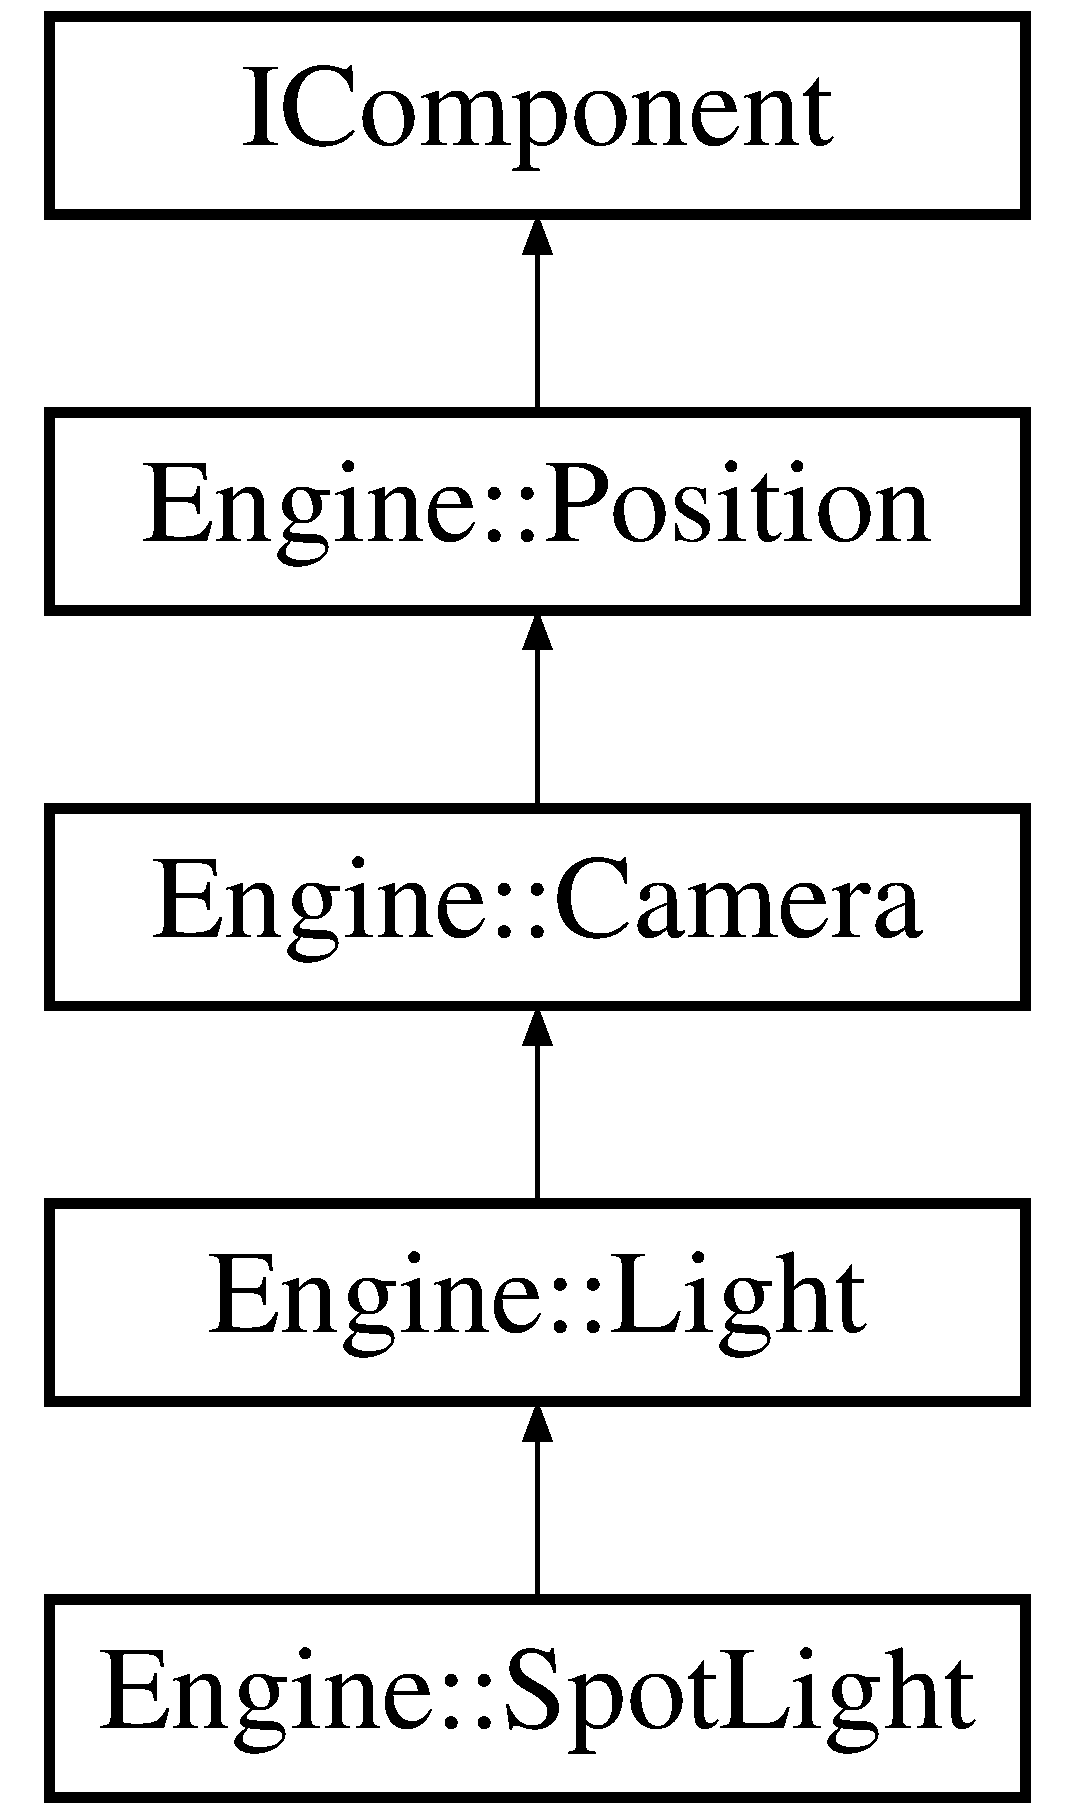
\includegraphics[height=5.000000cm]{classEngine_1_1Light}
\end{center}
\end{figure}
\subsection*{Public Member Functions}
\begin{DoxyCompactItemize}
\item 
\hyperlink{classEngine_1_1Light_a7ac5fa5177a3abf2114a4e513e1c3bc4}{Light} (void)
\begin{DoxyCompactList}\small\item\em \hyperlink{classEngine_1_1Light}{Light}. \end{DoxyCompactList}\item 
\hyperlink{classEngine_1_1Light_ae0cdf2a9d051a17d1ef0a8f4377be2d4}{Light} (const std\+::string \&light\+\_\+name)
\begin{DoxyCompactList}\small\item\em \hyperlink{classEngine_1_1Light}{Light}. \end{DoxyCompactList}\item 
void \hyperlink{classEngine_1_1Light_ae9fa0c29a7e422f6ac9227916c9392fb}{set\+Ambient} (const \hyperlink{classVector3}{Vector3f} \&ambient)
\begin{DoxyCompactList}\small\item\em set\+Ambient \end{DoxyCompactList}\item 
void \hyperlink{classEngine_1_1Light_a640cc033be739f52fd7675e76ee32208}{set\+Diffuse} (const \hyperlink{classVector3}{Vector3f} \&diffuse)
\begin{DoxyCompactList}\small\item\em set\+Diffuse \end{DoxyCompactList}\item 
void \hyperlink{classEngine_1_1Light_a95d38c9dae170c43334f2706391eab26}{set\+Specular} (const \hyperlink{classVector3}{Vector3f} \&specular)
\begin{DoxyCompactList}\small\item\em set\+Specular \end{DoxyCompactList}\item 
void \hyperlink{classEngine_1_1Light_ad0467c8eb3d393597fab68f4842100ec}{set\+Prefix} (const std\+::string \&prefix)
\begin{DoxyCompactList}\small\item\em set\+Prefix \end{DoxyCompactList}\item 
const \hyperlink{classVector3}{Vector3f} \& \hyperlink{classEngine_1_1Light_aa2ac9bcc2a394867c487a37f911ae1cb}{get\+Ambient} (void)
\begin{DoxyCompactList}\small\item\em get\+Ambient \end{DoxyCompactList}\item 
const \hyperlink{classVector3}{Vector3f} \& \hyperlink{classEngine_1_1Light_af7fb6a05515cee4f2b69e8c67fc665d6}{get\+Diffuse} (void)
\begin{DoxyCompactList}\small\item\em get\+Diffuse \end{DoxyCompactList}\item 
const \hyperlink{classVector3}{Vector3f} \& \hyperlink{classEngine_1_1Light_a79cf67acee1d7df1ccfd4a8e5147ce76}{get\+Specular} (void)
\begin{DoxyCompactList}\small\item\em get\+Specular \end{DoxyCompactList}\item 
virtual void \hyperlink{classEngine_1_1Light_a25c1173c8877e6900f508791cb98217a}{Shader\+Update} (int number, \hyperlink{classEngine_1_1IShader}{I\+Shader} $\ast$shader)
\begin{DoxyCompactList}\small\item\em Shader\+Update. \end{DoxyCompactList}\end{DoxyCompactItemize}
\subsection*{Protected Attributes}
\begin{DoxyCompactItemize}
\item 
\hypertarget{classEngine_1_1Light_ac679f82de845df19724535ddaf913aba}{}std\+::string {\bfseries m\+Prefix}\label{classEngine_1_1Light_ac679f82de845df19724535ddaf913aba}

\end{DoxyCompactItemize}
\subsection*{Additional Inherited Members}


\subsection{Detailed Description}
The \hyperlink{classEngine_1_1Light}{Light} class. 

Save \hyperlink{classEngine_1_1Light}{Light} data 

\subsection{Constructor \& Destructor Documentation}
\hypertarget{classEngine_1_1Light_a7ac5fa5177a3abf2114a4e513e1c3bc4}{}\index{Engine\+::\+Light@{Engine\+::\+Light}!Light@{Light}}
\index{Light@{Light}!Engine\+::\+Light@{Engine\+::\+Light}}
\subsubsection[{Light(void)}]{\setlength{\rightskip}{0pt plus 5cm}Light\+::\+Light (
\begin{DoxyParamCaption}
\item[{void}]{}
\end{DoxyParamCaption}
)\hspace{0.3cm}{\ttfamily [explicit]}}\label{classEngine_1_1Light_a7ac5fa5177a3abf2114a4e513e1c3bc4}


\hyperlink{classEngine_1_1Light}{Light}. 

Default Constructor \hypertarget{classEngine_1_1Light_ae0cdf2a9d051a17d1ef0a8f4377be2d4}{}\index{Engine\+::\+Light@{Engine\+::\+Light}!Light@{Light}}
\index{Light@{Light}!Engine\+::\+Light@{Engine\+::\+Light}}
\subsubsection[{Light(const std\+::string \&light\+\_\+name)}]{\setlength{\rightskip}{0pt plus 5cm}Engine\+::\+Light\+::\+Light (
\begin{DoxyParamCaption}
\item[{const std\+::string \&}]{light\+\_\+name}
\end{DoxyParamCaption}
)\hspace{0.3cm}{\ttfamily [explicit]}}\label{classEngine_1_1Light_ae0cdf2a9d051a17d1ef0a8f4377be2d4}


\hyperlink{classEngine_1_1Light}{Light}. 

Constructor with \hyperlink{classEngine_1_1Light}{Light} name 
\begin{DoxyParams}{Parameters}
{\em light\+\_\+name} & \\
\hline
\end{DoxyParams}


\subsection{Member Function Documentation}
\hypertarget{classEngine_1_1Light_aa2ac9bcc2a394867c487a37f911ae1cb}{}\index{Engine\+::\+Light@{Engine\+::\+Light}!get\+Ambient@{get\+Ambient}}
\index{get\+Ambient@{get\+Ambient}!Engine\+::\+Light@{Engine\+::\+Light}}
\subsubsection[{get\+Ambient(void)}]{\setlength{\rightskip}{0pt plus 5cm}const {\bf Vector3f} \& Light\+::get\+Ambient (
\begin{DoxyParamCaption}
\item[{void}]{}
\end{DoxyParamCaption}
)}\label{classEngine_1_1Light_aa2ac9bcc2a394867c487a37f911ae1cb}


get\+Ambient 

Return Ambient Color Vector \begin{DoxyReturn}{Returns}

\end{DoxyReturn}
\hypertarget{classEngine_1_1Light_af7fb6a05515cee4f2b69e8c67fc665d6}{}\index{Engine\+::\+Light@{Engine\+::\+Light}!get\+Diffuse@{get\+Diffuse}}
\index{get\+Diffuse@{get\+Diffuse}!Engine\+::\+Light@{Engine\+::\+Light}}
\subsubsection[{get\+Diffuse(void)}]{\setlength{\rightskip}{0pt plus 5cm}const {\bf Vector3f} \& Light\+::get\+Diffuse (
\begin{DoxyParamCaption}
\item[{void}]{}
\end{DoxyParamCaption}
)}\label{classEngine_1_1Light_af7fb6a05515cee4f2b69e8c67fc665d6}


get\+Diffuse 

Return Diffuse Color Vector \begin{DoxyReturn}{Returns}

\end{DoxyReturn}
\hypertarget{classEngine_1_1Light_a79cf67acee1d7df1ccfd4a8e5147ce76}{}\index{Engine\+::\+Light@{Engine\+::\+Light}!get\+Specular@{get\+Specular}}
\index{get\+Specular@{get\+Specular}!Engine\+::\+Light@{Engine\+::\+Light}}
\subsubsection[{get\+Specular(void)}]{\setlength{\rightskip}{0pt plus 5cm}const {\bf Vector3f} \& Light\+::get\+Specular (
\begin{DoxyParamCaption}
\item[{void}]{}
\end{DoxyParamCaption}
)}\label{classEngine_1_1Light_a79cf67acee1d7df1ccfd4a8e5147ce76}


get\+Specular 

Return Sepcular Color Vector \begin{DoxyReturn}{Returns}

\end{DoxyReturn}
\hypertarget{classEngine_1_1Light_ae9fa0c29a7e422f6ac9227916c9392fb}{}\index{Engine\+::\+Light@{Engine\+::\+Light}!set\+Ambient@{set\+Ambient}}
\index{set\+Ambient@{set\+Ambient}!Engine\+::\+Light@{Engine\+::\+Light}}
\subsubsection[{set\+Ambient(const Vector3f \&ambient)}]{\setlength{\rightskip}{0pt plus 5cm}void Light\+::set\+Ambient (
\begin{DoxyParamCaption}
\item[{const {\bf Vector3f} \&}]{ambient}
\end{DoxyParamCaption}
)}\label{classEngine_1_1Light_ae9fa0c29a7e422f6ac9227916c9392fb}


set\+Ambient 

Set Ambient Color Vector 
\begin{DoxyParams}{Parameters}
{\em ambient} & \\
\hline
\end{DoxyParams}
\hypertarget{classEngine_1_1Light_a640cc033be739f52fd7675e76ee32208}{}\index{Engine\+::\+Light@{Engine\+::\+Light}!set\+Diffuse@{set\+Diffuse}}
\index{set\+Diffuse@{set\+Diffuse}!Engine\+::\+Light@{Engine\+::\+Light}}
\subsubsection[{set\+Diffuse(const Vector3f \&diffuse)}]{\setlength{\rightskip}{0pt plus 5cm}void Light\+::set\+Diffuse (
\begin{DoxyParamCaption}
\item[{const {\bf Vector3f} \&}]{diffuse}
\end{DoxyParamCaption}
)}\label{classEngine_1_1Light_a640cc033be739f52fd7675e76ee32208}


set\+Diffuse 

Set Diffuse Color Vector 
\begin{DoxyParams}{Parameters}
{\em diffuse} & \\
\hline
\end{DoxyParams}
\hypertarget{classEngine_1_1Light_ad0467c8eb3d393597fab68f4842100ec}{}\index{Engine\+::\+Light@{Engine\+::\+Light}!set\+Prefix@{set\+Prefix}}
\index{set\+Prefix@{set\+Prefix}!Engine\+::\+Light@{Engine\+::\+Light}}
\subsubsection[{set\+Prefix(const std\+::string \&prefix)}]{\setlength{\rightskip}{0pt plus 5cm}void Light\+::set\+Prefix (
\begin{DoxyParamCaption}
\item[{const std\+::string \&}]{prefix}
\end{DoxyParamCaption}
)}\label{classEngine_1_1Light_ad0467c8eb3d393597fab68f4842100ec}


set\+Prefix 

Set Prefix for \hyperlink{classEngine_1_1Shader}{Shader} 
\begin{DoxyParams}{Parameters}
{\em prefix} & \\
\hline
\end{DoxyParams}
\hypertarget{classEngine_1_1Light_a95d38c9dae170c43334f2706391eab26}{}\index{Engine\+::\+Light@{Engine\+::\+Light}!set\+Specular@{set\+Specular}}
\index{set\+Specular@{set\+Specular}!Engine\+::\+Light@{Engine\+::\+Light}}
\subsubsection[{set\+Specular(const Vector3f \&specular)}]{\setlength{\rightskip}{0pt plus 5cm}void Light\+::set\+Specular (
\begin{DoxyParamCaption}
\item[{const {\bf Vector3f} \&}]{specular}
\end{DoxyParamCaption}
)}\label{classEngine_1_1Light_a95d38c9dae170c43334f2706391eab26}


set\+Specular 

Set Specular Color Vector 
\begin{DoxyParams}{Parameters}
{\em specular} & \\
\hline
\end{DoxyParams}
\hypertarget{classEngine_1_1Light_a25c1173c8877e6900f508791cb98217a}{}\index{Engine\+::\+Light@{Engine\+::\+Light}!Shader\+Update@{Shader\+Update}}
\index{Shader\+Update@{Shader\+Update}!Engine\+::\+Light@{Engine\+::\+Light}}
\subsubsection[{Shader\+Update(int number, I\+Shader $\ast$shader)}]{\setlength{\rightskip}{0pt plus 5cm}void Light\+::\+Shader\+Update (
\begin{DoxyParamCaption}
\item[{int}]{number, }
\item[{{\bf I\+Shader} $\ast$}]{shader}
\end{DoxyParamCaption}
)\hspace{0.3cm}{\ttfamily [virtual]}}\label{classEngine_1_1Light_a25c1173c8877e6900f508791cb98217a}


Shader\+Update. 

\hyperlink{classEngine_1_1Shader}{Shader} Update 
\begin{DoxyParams}{Parameters}
{\em shader} & \\
\hline
\end{DoxyParams}


Reimplemented in \hyperlink{classEngine_1_1SpotLight_aa6f5b9024c2cab0fab556e4f66611fa4}{Engine\+::\+Spot\+Light}.



The documentation for this class was generated from the following files\+:\begin{DoxyCompactItemize}
\item 
include/\+Container/light.\+h\item 
Container/Light.\+cpp\end{DoxyCompactItemize}

\hypertarget{classEngine_1_1LightManager}{}\section{Engine\+:\+:Light\+Manager Class Reference}
\label{classEngine_1_1LightManager}\index{Engine\+::\+Light\+Manager@{Engine\+::\+Light\+Manager}}


The \hyperlink{classEngine_1_1LightManager}{Light\+Manager} class.  




{\ttfamily \#include $<$lightmanager.\+h$>$}

\subsection*{Public Member Functions}
\begin{DoxyCompactItemize}
\item 
\hypertarget{classEngine_1_1LightManager_ac886d9357ad312c625066e95d3cfd14e}{}void {\bfseries set\+Bias\+\_\+\+Test} (float value)\label{classEngine_1_1LightManager_ac886d9357ad312c625066e95d3cfd14e}

\item 
\hypertarget{classEngine_1_1LightManager_a8fd0da62e739ab9d4931c008a7c16475}{}float {\bfseries get\+Bias\+\_\+\+Test} (void)\label{classEngine_1_1LightManager_a8fd0da62e739ab9d4931c008a7c16475}

\item 
\hyperlink{classEngine_1_1Light}{Light} $\ast$ \hyperlink{classEngine_1_1LightManager_a1fc44ab503b283155ca0541e033380bd}{create\+Light} (const string \&light\+\_\+name)
\begin{DoxyCompactList}\small\item\em create\+Light \end{DoxyCompactList}\item 
\hypertarget{classEngine_1_1LightManager_a3900dcd2b60f42d1028ab18b1d50fad6}{}\hyperlink{classEngine_1_1SpotLight}{Spot\+Light} $\ast$ {\bfseries create\+Spot\+Light} (const string \&light\+\_\+name)\label{classEngine_1_1LightManager_a3900dcd2b60f42d1028ab18b1d50fad6}

\item 
void \hyperlink{classEngine_1_1LightManager_a410c2c0a2b518dc89be34788bdc9d22c}{remove} (const string \&light\+\_\+name)
\begin{DoxyCompactList}\small\item\em remove \end{DoxyCompactList}\item 
\hyperlink{classEngine_1_1Light}{Light} $\ast$ \hyperlink{classEngine_1_1LightManager_ab516482393ea525e57a24b6ccfa2b32f}{get\+Light} (const std\+::string \&light\+\_\+name)
\begin{DoxyCompactList}\small\item\em get\+Light \end{DoxyCompactList}\item 
\hypertarget{classEngine_1_1LightManager_a64c342a479210b8f4211aa2880aa05c6}{}\hyperlink{classEngine_1_1SpotLight}{Spot\+Light} $\ast$ {\bfseries get\+Spot\+Light} (const std\+::string \&spotlight\+\_\+name)\label{classEngine_1_1LightManager_a64c342a479210b8f4211aa2880aa05c6}

\item 
Lights \hyperlink{classEngine_1_1LightManager_af8b211420f10d9b29d72114a69ce5175}{get\+Lights} (void)
\begin{DoxyCompactList}\small\item\em get\+Lights \end{DoxyCompactList}\item 
Spot\+Lights \hyperlink{classEngine_1_1LightManager_a3e0b088762961ea2f94d56f78ed2ee8c}{get\+Spot\+Lights} (void)
\begin{DoxyCompactList}\small\item\em get\+Spot\+Lights \end{DoxyCompactList}\end{DoxyCompactItemize}
\subsection*{Static Public Member Functions}
\begin{DoxyCompactItemize}
\item 
static \hyperlink{classEngine_1_1LightManager}{Light\+Manager} $\ast$ \hyperlink{classEngine_1_1LightManager_a875c588f08141aca1aff38ae0a1c1b1e}{get\+Singleton\+Ptr} (void)
\begin{DoxyCompactList}\small\item\em get\+Singleton\+Ptr \end{DoxyCompactList}\end{DoxyCompactItemize}


\subsection{Detailed Description}
The \hyperlink{classEngine_1_1LightManager}{Light\+Manager} class. 

Management of Lights


\begin{DoxyItemize}
\item create \hyperlink{classEngine_1_1Light}{Light} objects
\item delete \hyperlink{classEngine_1_1Light}{Light} objects 
\end{DoxyItemize}

\subsection{Member Function Documentation}
\hypertarget{classEngine_1_1LightManager_a1fc44ab503b283155ca0541e033380bd}{}\index{Engine\+::\+Light\+Manager@{Engine\+::\+Light\+Manager}!create\+Light@{create\+Light}}
\index{create\+Light@{create\+Light}!Engine\+::\+Light\+Manager@{Engine\+::\+Light\+Manager}}
\subsubsection[{create\+Light(const string \&light\+\_\+name)}]{\setlength{\rightskip}{0pt plus 5cm}{\bf Light} $\ast$ Light\+Manager\+::create\+Light (
\begin{DoxyParamCaption}
\item[{const string \&}]{light\+\_\+name}
\end{DoxyParamCaption}
)}\label{classEngine_1_1LightManager_a1fc44ab503b283155ca0541e033380bd}


create\+Light 

Create a new \hyperlink{classEngine_1_1Light}{Light} with Name 
\begin{DoxyParams}{Parameters}
{\em light\+\_\+name} & \\
\hline
\end{DoxyParams}
\begin{DoxyReturn}{Returns}

\end{DoxyReturn}
\hypertarget{classEngine_1_1LightManager_ab516482393ea525e57a24b6ccfa2b32f}{}\index{Engine\+::\+Light\+Manager@{Engine\+::\+Light\+Manager}!get\+Light@{get\+Light}}
\index{get\+Light@{get\+Light}!Engine\+::\+Light\+Manager@{Engine\+::\+Light\+Manager}}
\subsubsection[{get\+Light(const std\+::string \&light\+\_\+name)}]{\setlength{\rightskip}{0pt plus 5cm}{\bf Light} $\ast$ Light\+Manager\+::get\+Light (
\begin{DoxyParamCaption}
\item[{const std\+::string \&}]{light\+\_\+name}
\end{DoxyParamCaption}
)}\label{classEngine_1_1LightManager_ab516482393ea525e57a24b6ccfa2b32f}


get\+Light 

Return \hyperlink{classEngine_1_1Light}{Light} object by Name 
\begin{DoxyParams}{Parameters}
{\em light\+\_\+name} & \\
\hline
\end{DoxyParams}
\begin{DoxyReturn}{Returns}

\end{DoxyReturn}
\hypertarget{classEngine_1_1LightManager_af8b211420f10d9b29d72114a69ce5175}{}\index{Engine\+::\+Light\+Manager@{Engine\+::\+Light\+Manager}!get\+Lights@{get\+Lights}}
\index{get\+Lights@{get\+Lights}!Engine\+::\+Light\+Manager@{Engine\+::\+Light\+Manager}}
\subsubsection[{get\+Lights(void)}]{\setlength{\rightskip}{0pt plus 5cm}Lights Light\+Manager\+::get\+Lights (
\begin{DoxyParamCaption}
\item[{void}]{}
\end{DoxyParamCaption}
)}\label{classEngine_1_1LightManager_af8b211420f10d9b29d72114a69ce5175}


get\+Lights 

Return a List of Lights \begin{DoxyReturn}{Returns}

\end{DoxyReturn}
\hypertarget{classEngine_1_1LightManager_a875c588f08141aca1aff38ae0a1c1b1e}{}\index{Engine\+::\+Light\+Manager@{Engine\+::\+Light\+Manager}!get\+Singleton\+Ptr@{get\+Singleton\+Ptr}}
\index{get\+Singleton\+Ptr@{get\+Singleton\+Ptr}!Engine\+::\+Light\+Manager@{Engine\+::\+Light\+Manager}}
\subsubsection[{get\+Singleton\+Ptr(void)}]{\setlength{\rightskip}{0pt plus 5cm}{\bf Light\+Manager} $\ast$ Light\+Manager\+::get\+Singleton\+Ptr (
\begin{DoxyParamCaption}
\item[{void}]{}
\end{DoxyParamCaption}
)\hspace{0.3cm}{\ttfamily [static]}}\label{classEngine_1_1LightManager_a875c588f08141aca1aff38ae0a1c1b1e}


get\+Singleton\+Ptr 

Return \hyperlink{classEngine_1_1LightManager}{Light\+Manager} Instance \begin{DoxyReturn}{Returns}

\end{DoxyReturn}
\hypertarget{classEngine_1_1LightManager_a3e0b088762961ea2f94d56f78ed2ee8c}{}\index{Engine\+::\+Light\+Manager@{Engine\+::\+Light\+Manager}!get\+Spot\+Lights@{get\+Spot\+Lights}}
\index{get\+Spot\+Lights@{get\+Spot\+Lights}!Engine\+::\+Light\+Manager@{Engine\+::\+Light\+Manager}}
\subsubsection[{get\+Spot\+Lights(void)}]{\setlength{\rightskip}{0pt plus 5cm}Spot\+Lights Light\+Manager\+::get\+Spot\+Lights (
\begin{DoxyParamCaption}
\item[{void}]{}
\end{DoxyParamCaption}
)}\label{classEngine_1_1LightManager_a3e0b088762961ea2f94d56f78ed2ee8c}


get\+Spot\+Lights 

\begin{DoxyReturn}{Returns}

\end{DoxyReturn}
\hypertarget{classEngine_1_1LightManager_a410c2c0a2b518dc89be34788bdc9d22c}{}\index{Engine\+::\+Light\+Manager@{Engine\+::\+Light\+Manager}!remove@{remove}}
\index{remove@{remove}!Engine\+::\+Light\+Manager@{Engine\+::\+Light\+Manager}}
\subsubsection[{remove(const string \&light\+\_\+name)}]{\setlength{\rightskip}{0pt plus 5cm}void Light\+Manager\+::remove (
\begin{DoxyParamCaption}
\item[{const string \&}]{light\+\_\+name}
\end{DoxyParamCaption}
)}\label{classEngine_1_1LightManager_a410c2c0a2b518dc89be34788bdc9d22c}


remove 

Remove \hyperlink{classEngine_1_1Light}{Light} object by Name 
\begin{DoxyParams}{Parameters}
{\em light\+\_\+name} & \\
\hline
\end{DoxyParams}


The documentation for this class was generated from the following files\+:\begin{DoxyCompactItemize}
\item 
include/\+Manager/lightmanager.\+h\item 
Engine/\+Manager/Light\+Manager.\+cpp\end{DoxyCompactItemize}

\hypertarget{classEngine_1_1LogManager}{}\section{Engine\+:\+:Log\+Manager Class Reference}
\label{classEngine_1_1LogManager}\index{Engine\+::\+Log\+Manager@{Engine\+::\+Log\+Manager}}


The \hyperlink{classEngine_1_1LogManager}{Log\+Manager} class.  




{\ttfamily \#include $<$logmanager.\+h$>$}

\subsection*{Public Types}
\begin{DoxyCompactItemize}
\item 
\hypertarget{classEngine_1_1LogManager_a540739bc2fa1ac620163c76ebda2c9fe}{}enum {\bfseries Level} \{ \\*
{\bfseries L\+O\+G\+\_\+\+I\+N\+F\+O}, 
{\bfseries L\+O\+G\+\_\+\+W\+A\+R\+N\+I\+N\+G}, 
{\bfseries L\+O\+G\+\_\+\+E\+R\+R\+O\+R}, 
{\bfseries L\+O\+G\+\_\+\+D\+E\+B\+U\+G}, 
\\*
{\bfseries L\+O\+G\+\_\+\+E\+X\+C\+E\+P\+T\+I\+O\+N}
 \}\label{classEngine_1_1LogManager_a540739bc2fa1ac620163c76ebda2c9fe}

\end{DoxyCompactItemize}
\subsection*{Static Public Member Functions}
\begin{DoxyCompactItemize}
\item 
static \hyperlink{classEngine_1_1LogManager}{Log\+Manager} $\ast$ \hyperlink{classEngine_1_1LogManager_a5ab655fd02bb6c0ae2cde3be4794375f}{get\+Singleton\+Ptr} (void)
\begin{DoxyCompactList}\small\item\em get\+Singleton\+Ptr \end{DoxyCompactList}\item 
static void \hyperlink{classEngine_1_1LogManager_acdc0eb4baacb4f3b018698665d398c6a}{log} (Level level, stringstream \&message)  throw ( std\+::runtime\+\_\+error )
\begin{DoxyCompactList}\small\item\em log \end{DoxyCompactList}\item 
\hypertarget{classEngine_1_1LogManager_ab3977fc0bd8b1df870e96588b082afa8}{}static void {\bfseries log} (Level level, const std\+::string \&message)  throw ( std\+::runtime\+\_\+error )\label{classEngine_1_1LogManager_ab3977fc0bd8b1df870e96588b082afa8}

\item 
\hypertarget{classEngine_1_1LogManager_a17b9d4159c82a218d4db38430490d492}{}static void {\bfseries Frame\+Buffer\+Check\+Status} (const std\+::string \&information)\label{classEngine_1_1LogManager_a17b9d4159c82a218d4db38430490d492}

\item 
static void \hyperlink{classEngine_1_1LogManager_a00096d95e37109861617033fd26a9e91}{get\+Error} (const std\+::string \&information)
\begin{DoxyCompactList}\small\item\em \hyperlink{classEngine_1_1LogManager_a00096d95e37109861617033fd26a9e91}{Log\+Manager\+::get\+Error}. \end{DoxyCompactList}\item 
\hypertarget{classEngine_1_1LogManager_a2c386f3ab894bbd5c1c337197fcfb6d9}{}static void {\bfseries print\+Array} (float $\ast$pointer, int size)\label{classEngine_1_1LogManager_a2c386f3ab894bbd5c1c337197fcfb6d9}

\item 
\hypertarget{classEngine_1_1LogManager_a0f64948d2f9f79627fbbfcfeb1e1527f}{}static void {\bfseries print\+Pointer} (void $\ast$pointer)\label{classEngine_1_1LogManager_a0f64948d2f9f79627fbbfcfeb1e1527f}

\item 
\hypertarget{classEngine_1_1LogManager_ae1d7f155f7c9a06330e8d4f712333a95}{}static void {\bfseries print\+To\+File} (const std\+::string \&file\+\_\+name, const std\+::string \&message)\label{classEngine_1_1LogManager_ae1d7f155f7c9a06330e8d4f712333a95}

\end{DoxyCompactItemize}


\subsection{Detailed Description}
The \hyperlink{classEngine_1_1LogManager}{Log\+Manager} class. 

Logger -\/ Print Log\+Message into Console 

\subsection{Member Function Documentation}
\hypertarget{classEngine_1_1LogManager_a00096d95e37109861617033fd26a9e91}{}\index{Engine\+::\+Log\+Manager@{Engine\+::\+Log\+Manager}!get\+Error@{get\+Error}}
\index{get\+Error@{get\+Error}!Engine\+::\+Log\+Manager@{Engine\+::\+Log\+Manager}}
\subsubsection[{get\+Error(const std\+::string \&information)}]{\setlength{\rightskip}{0pt plus 5cm}void Log\+Manager\+::get\+Error (
\begin{DoxyParamCaption}
\item[{const std\+::string \&}]{info}
\end{DoxyParamCaption}
)\hspace{0.3cm}{\ttfamily [static]}}\label{classEngine_1_1LogManager_a00096d95e37109861617033fd26a9e91}


\hyperlink{classEngine_1_1LogManager_a00096d95e37109861617033fd26a9e91}{Log\+Manager\+::get\+Error}. 

Check Open\+G\+L Errors 
\begin{DoxyParams}{Parameters}
{\em info} & \\
\hline
\end{DoxyParams}
\hypertarget{classEngine_1_1LogManager_a5ab655fd02bb6c0ae2cde3be4794375f}{}\index{Engine\+::\+Log\+Manager@{Engine\+::\+Log\+Manager}!get\+Singleton\+Ptr@{get\+Singleton\+Ptr}}
\index{get\+Singleton\+Ptr@{get\+Singleton\+Ptr}!Engine\+::\+Log\+Manager@{Engine\+::\+Log\+Manager}}
\subsubsection[{get\+Singleton\+Ptr(void)}]{\setlength{\rightskip}{0pt plus 5cm}{\bf Log\+Manager} $\ast$ Log\+Manager\+::get\+Singleton\+Ptr (
\begin{DoxyParamCaption}
\item[{void}]{}
\end{DoxyParamCaption}
)\hspace{0.3cm}{\ttfamily [static]}}\label{classEngine_1_1LogManager_a5ab655fd02bb6c0ae2cde3be4794375f}


get\+Singleton\+Ptr 

Return \hyperlink{classEngine_1_1LogManager}{Log\+Manager} Instance \begin{DoxyReturn}{Returns}

\end{DoxyReturn}
\hypertarget{classEngine_1_1LogManager_acdc0eb4baacb4f3b018698665d398c6a}{}\index{Engine\+::\+Log\+Manager@{Engine\+::\+Log\+Manager}!log@{log}}
\index{log@{log}!Engine\+::\+Log\+Manager@{Engine\+::\+Log\+Manager}}
\subsubsection[{log(\+Level level, stringstream \&message)}]{\setlength{\rightskip}{0pt plus 5cm}void Log\+Manager\+::log (
\begin{DoxyParamCaption}
\item[{Level}]{level, }
\item[{stringstream \&}]{message}
\end{DoxyParamCaption}
) throw  std\+::runtime\+\_\+error) \hspace{0.3cm}{\ttfamily [static]}}\label{classEngine_1_1LogManager_acdc0eb4baacb4f3b018698665d398c6a}


log 

Print Log Message 
\begin{DoxyParams}{Parameters}
{\em level} & \\
\hline
{\em message} & \\
\hline
\end{DoxyParams}


The documentation for this class was generated from the following files\+:\begin{DoxyCompactItemize}
\item 
include/\+Manager/logmanager.\+h\item 
Engine/\+Manager/Log\+Manager.\+cpp\end{DoxyCompactItemize}

\hypertarget{classEngine_1_1Material}{}\section{Engine\+:\+:Material Class Reference}
\label{classEngine_1_1Material}\index{Engine\+::\+Material@{Engine\+::\+Material}}
Inheritance diagram for Engine\+:\+:Material\+:\begin{figure}[H]
\begin{center}
\leavevmode
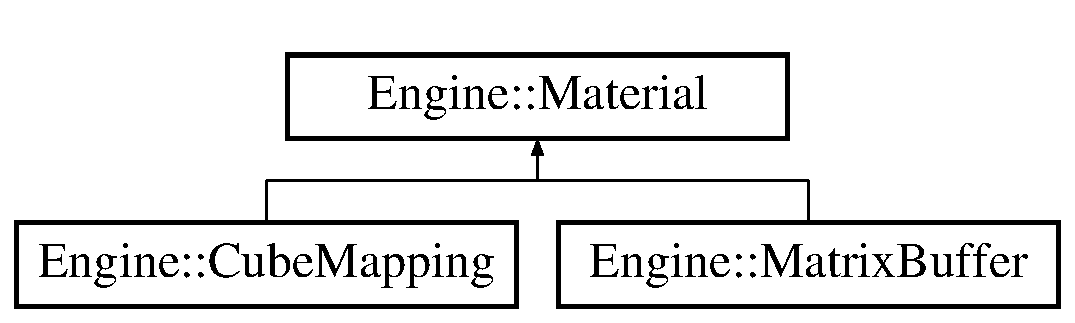
\includegraphics[height=2.000000cm]{classEngine_1_1Material}
\end{center}
\end{figure}
\subsection*{Public Member Functions}
\begin{DoxyCompactItemize}
\item 
\hypertarget{classEngine_1_1Material_aaca068d634155c8c038d9e398a4820c2}{}{\bfseries Material} (\hyperlink{classEngine_1_1Entity}{Entity} $\ast$entity)\label{classEngine_1_1Material_aaca068d634155c8c038d9e398a4820c2}

\item 
\hypertarget{classEngine_1_1Material_a8a51ad4fb9347e1ce720bfbbb37fafa0}{}virtual void {\bfseries enable} (int texture\+\_\+unit)=0\label{classEngine_1_1Material_a8a51ad4fb9347e1ce720bfbbb37fafa0}

\end{DoxyCompactItemize}
\subsection*{Protected Attributes}
\begin{DoxyCompactItemize}
\item 
\hypertarget{classEngine_1_1Material_a1e5cc0152e801d6177f47d92e763fab1}{}\hyperlink{classEngine_1_1Entity}{Entity} $\ast$ {\bfseries m\+Entity}\label{classEngine_1_1Material_a1e5cc0152e801d6177f47d92e763fab1}

\end{DoxyCompactItemize}


The documentation for this class was generated from the following file\+:\begin{DoxyCompactItemize}
\item 
include/\+Container/material.\+h\end{DoxyCompactItemize}

\hypertarget{classEngine_1_1MatrixBuffer}{}\section{Engine\+:\+:Matrix\+Buffer Class Reference}
\label{classEngine_1_1MatrixBuffer}\index{Engine\+::\+Matrix\+Buffer@{Engine\+::\+Matrix\+Buffer}}
Inheritance diagram for Engine\+:\+:Matrix\+Buffer\+:\begin{figure}[H]
\begin{center}
\leavevmode
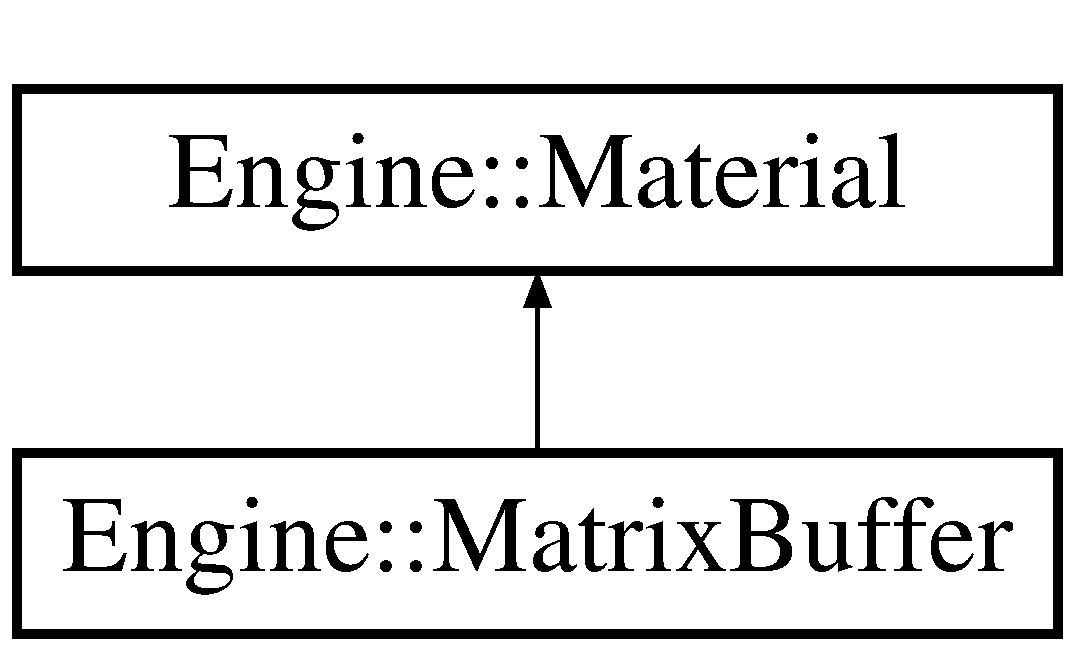
\includegraphics[height=2.000000cm]{classEngine_1_1MatrixBuffer}
\end{center}
\end{figure}
\subsection*{Public Member Functions}
\begin{DoxyCompactItemize}
\item 
\hypertarget{classEngine_1_1MatrixBuffer_a6efea6edf2c22333a08e70a39464d97f}{}{\bfseries Matrix\+Buffer} (\hyperlink{classEngine_1_1Entity}{Entity} $\ast$entity)\label{classEngine_1_1MatrixBuffer_a6efea6edf2c22333a08e70a39464d97f}

\item 
\hypertarget{classEngine_1_1MatrixBuffer_ae1956d5ccefd322ced2d1ae5bbecad5b}{}void {\bfseries create} (int tbo\+\_\+draws, Vector3fv tbo\+\_\+data, bool update\+\_\+flag)\label{classEngine_1_1MatrixBuffer_ae1956d5ccefd322ced2d1ae5bbecad5b}

\item 
\hypertarget{classEngine_1_1MatrixBuffer_a498dae58a6e73ccea9abbcd942b9c514}{}void {\bfseries set\+T\+B\+O\+Data} (Vector3fv tbo\+\_\+data)\label{classEngine_1_1MatrixBuffer_a498dae58a6e73ccea9abbcd942b9c514}

\item 
\hypertarget{classEngine_1_1MatrixBuffer_a7a012f4da7b821d55dc4f7ff68a388f0}{}void {\bfseries enable} (int texture\+\_\+unit)\label{classEngine_1_1MatrixBuffer_a7a012f4da7b821d55dc4f7ff68a388f0}

\end{DoxyCompactItemize}
\subsection*{Additional Inherited Members}


The documentation for this class was generated from the following files\+:\begin{DoxyCompactItemize}
\item 
include/\+Material/matrixbuffer.\+h\item 
Container/\+Material/Matrix\+Buffer.\+cpp\end{DoxyCompactItemize}

\hypertarget{classEngine_1_1Mesh}{}\section{Engine\+:\+:Mesh Class Reference}
\label{classEngine_1_1Mesh}\index{Engine\+::\+Mesh@{Engine\+::\+Mesh}}


The \hyperlink{classEngine_1_1Mesh}{Mesh} class.  




{\ttfamily \#include $<$mesh.\+h$>$}

Inheritance diagram for Engine\+:\+:Mesh\+:\begin{figure}[H]
\begin{center}
\leavevmode
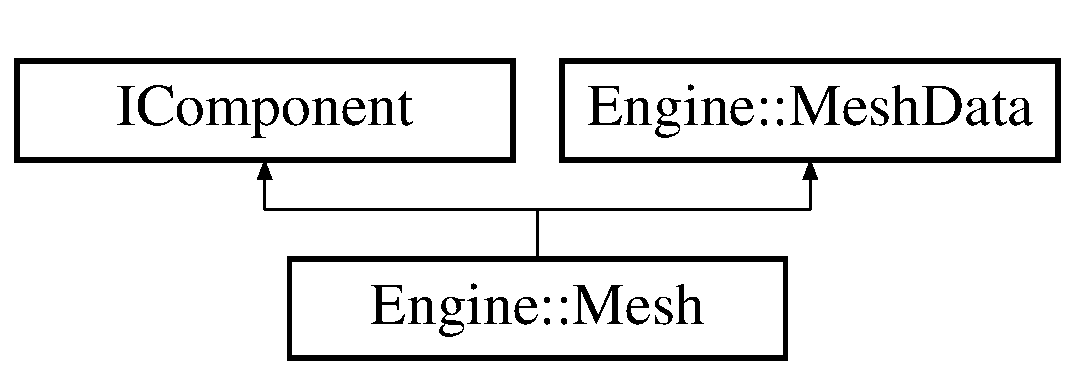
\includegraphics[height=2.000000cm]{classEngine_1_1Mesh}
\end{center}
\end{figure}
\subsection*{Public Member Functions}
\begin{DoxyCompactItemize}
\item 
void \hyperlink{classEngine_1_1Mesh_a91b3647bd0d2c7c826e3b74d3748c05d}{set\+G\+L\+Vertex\+Array\+Object} (\hyperlink{classEngine_1_1GLVertexArrayObject}{G\+L\+Vertex\+Array\+Object} $\ast$vao\+\_\+object)
\begin{DoxyCompactList}\small\item\em set\+G\+L\+Vertex\+Array\+Object \end{DoxyCompactList}\item 
\hyperlink{classEngine_1_1GLVertexArrayObject}{G\+L\+Vertex\+Array\+Object} $\ast$ \hyperlink{classEngine_1_1Mesh_a3b1be4f7909621d4bb2385907a10a568}{get\+Vertex\+Array\+Object} (void)
\begin{DoxyCompactList}\small\item\em get\+Vertex\+Array\+Object \end{DoxyCompactList}\item 
\hypertarget{classEngine_1_1Mesh_a83800bea9663aef8eeb9bc343b5a55ca}{}void {\bfseries Draw} (void)\label{classEngine_1_1Mesh_a83800bea9663aef8eeb9bc343b5a55ca}

\item 
\hypertarget{classEngine_1_1Mesh_a5c1bc4e3fec668c7802a3d0192e81586}{}void {\bfseries Draw\+Elements} (void)\label{classEngine_1_1Mesh_a5c1bc4e3fec668c7802a3d0192e81586}

\item 
\hypertarget{classEngine_1_1Mesh_ac3c6ca7b99072f370be0f845307792f7}{}void {\bfseries Draw\+Elements\+Indirect} (int drawcount)\label{classEngine_1_1Mesh_ac3c6ca7b99072f370be0f845307792f7}

\item 
\hypertarget{classEngine_1_1Mesh_a7f360c77bda20f2744eb25b67d6ad467}{}void {\bfseries Draw\+Elements\+Instanced} (int drawcount)\label{classEngine_1_1Mesh_a7f360c77bda20f2744eb25b67d6ad467}

\end{DoxyCompactItemize}
\subsection*{Additional Inherited Members}


\subsection{Detailed Description}
The \hyperlink{classEngine_1_1Mesh}{Mesh} class. 

\subsection{Member Function Documentation}
\hypertarget{classEngine_1_1Mesh_a3b1be4f7909621d4bb2385907a10a568}{}\index{Engine\+::\+Mesh@{Engine\+::\+Mesh}!get\+Vertex\+Array\+Object@{get\+Vertex\+Array\+Object}}
\index{get\+Vertex\+Array\+Object@{get\+Vertex\+Array\+Object}!Engine\+::\+Mesh@{Engine\+::\+Mesh}}
\subsubsection[{get\+Vertex\+Array\+Object(void)}]{\setlength{\rightskip}{0pt plus 5cm}{\bf G\+L\+Vertex\+Array\+Object} $\ast$ Mesh\+::get\+Vertex\+Array\+Object (
\begin{DoxyParamCaption}
\item[{void}]{}
\end{DoxyParamCaption}
)}\label{classEngine_1_1Mesh_a3b1be4f7909621d4bb2385907a10a568}


get\+Vertex\+Array\+Object 

Get V\+A\+O \begin{DoxyReturn}{Returns}

\end{DoxyReturn}
\hypertarget{classEngine_1_1Mesh_a91b3647bd0d2c7c826e3b74d3748c05d}{}\index{Engine\+::\+Mesh@{Engine\+::\+Mesh}!set\+G\+L\+Vertex\+Array\+Object@{set\+G\+L\+Vertex\+Array\+Object}}
\index{set\+G\+L\+Vertex\+Array\+Object@{set\+G\+L\+Vertex\+Array\+Object}!Engine\+::\+Mesh@{Engine\+::\+Mesh}}
\subsubsection[{set\+G\+L\+Vertex\+Array\+Object(\+G\+L\+Vertex\+Array\+Object $\ast$vao\+\_\+object)}]{\setlength{\rightskip}{0pt plus 5cm}void Mesh\+::set\+G\+L\+Vertex\+Array\+Object (
\begin{DoxyParamCaption}
\item[{{\bf G\+L\+Vertex\+Array\+Object} $\ast$}]{vao\+\_\+object}
\end{DoxyParamCaption}
)}\label{classEngine_1_1Mesh_a91b3647bd0d2c7c826e3b74d3748c05d}


set\+G\+L\+Vertex\+Array\+Object 

Set V\+A\+O 
\begin{DoxyParams}{Parameters}
{\em vao\+\_\+object} & \\
\hline
\end{DoxyParams}


The documentation for this class was generated from the following files\+:\begin{DoxyCompactItemize}
\item 
include/\+Container/mesh.\+h\item 
Container/Mesh.\+cpp\end{DoxyCompactItemize}

\hypertarget{classEngine_1_1MeshData}{}\section{Engine\+:\+:Mesh\+Data Class Reference}
\label{classEngine_1_1MeshData}\index{Engine\+::\+Mesh\+Data@{Engine\+::\+Mesh\+Data}}


The \hyperlink{classEngine_1_1MeshData}{Mesh\+Data} -\/ abstract class.  




{\ttfamily \#include $<$meshdata.\+h$>$}

Inheritance diagram for Engine\+:\+:Mesh\+Data\+:\begin{figure}[H]
\begin{center}
\leavevmode
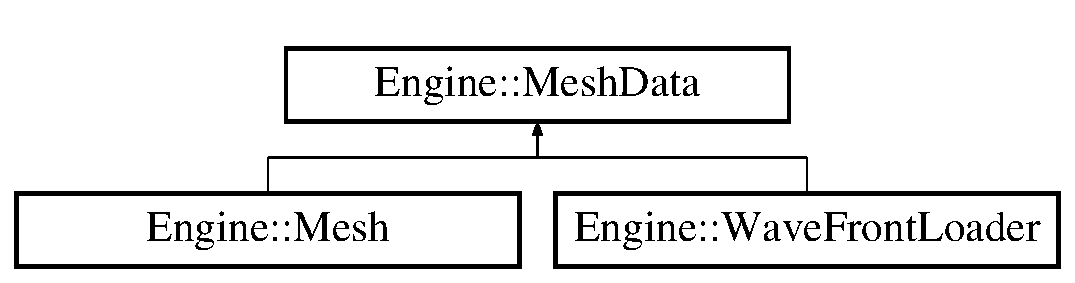
\includegraphics[height=2.000000cm]{classEngine_1_1MeshData}
\end{center}
\end{figure}
\subsection*{Public Member Functions}
\begin{DoxyCompactItemize}
\item 
Group\+Id\+List \hyperlink{classEngine_1_1MeshData_a5e1b9108ca9e19e5a981fec9cd8a351f}{get\+Group\+Id\+List} (void) const 
\begin{DoxyCompactList}\small\item\em \hyperlink{classEngine_1_1MeshData_a5e1b9108ca9e19e5a981fec9cd8a351f}{Mesh\+Data\+::get\+Group\+Id\+List}. \end{DoxyCompactList}\item 
Vertex\+Groups \hyperlink{classEngine_1_1MeshData_a29232cd601a0480433f23b9faf2a1fa3}{get\+Vertex\+Groups} (void) const 
\begin{DoxyCompactList}\small\item\em get\+Vertex\+Groups \end{DoxyCompactList}\item 
Vector3fv \hyperlink{classEngine_1_1MeshData_a2f24a9508fec6c078f8dff74a64b3566}{get\+Vertices} (void) const 
\begin{DoxyCompactList}\small\item\em get\+Vertices \end{DoxyCompactList}\item 
Vector3fv \hyperlink{classEngine_1_1MeshData_aab08fdc17ec7f531cd6a5c006ac7b607}{get\+Normals} (void) const 
\begin{DoxyCompactList}\small\item\em get\+Normals \end{DoxyCompactList}\item 
Vector2fv \hyperlink{classEngine_1_1MeshData_a8c8c11d0c12e2fafdddbe05efc6057f3}{get\+Texcoord} (void) const 
\begin{DoxyCompactList}\small\item\em get\+Texcoord \end{DoxyCompactList}\item 
Vector3fv \hyperlink{classEngine_1_1MeshData_af8a7aceef507044cf0fa7b385df27d14}{get\+Index\+Vertex} (void) const 
\begin{DoxyCompactList}\small\item\em get\+Index\+Vertex \end{DoxyCompactList}\item 
Vector3fv \hyperlink{classEngine_1_1MeshData_af59825e8b56b0858d33132b0b2032e26}{get\+Index\+Tex\+Coords} (void) const 
\begin{DoxyCompactList}\small\item\em get\+Index\+Tex\+Coords \end{DoxyCompactList}\item 
Vector3fv \hyperlink{classEngine_1_1MeshData_a6f0bce28267f02e0c34d11b7687fe0be}{get\+Index\+Normals} (void) const 
\begin{DoxyCompactList}\small\item\em get\+Index\+Normals \end{DoxyCompactList}\item 
Vector3fv \hyperlink{classEngine_1_1MeshData_aafbb445af15c51bb2faa3f0c6a3c0723}{get\+Original\+Vertices} (void) const 
\begin{DoxyCompactList}\small\item\em get\+Original\+Vertices \end{DoxyCompactList}\item 
Vector3fv \hyperlink{classEngine_1_1MeshData_a3c212f964ee82ed741fdf750db3374d1}{get\+Original\+Normals} (void) const 
\begin{DoxyCompactList}\small\item\em get\+Original\+Normals \end{DoxyCompactList}\item 
Vector2fv \hyperlink{classEngine_1_1MeshData_a6f380528398deb5f1ba4a8e626feb7ec}{get\+Original\+Tex\+Coords} (void) const 
\begin{DoxyCompactList}\small\item\em get\+Original\+Tex\+Coords \end{DoxyCompactList}\item 
Vector3fv \hyperlink{classEngine_1_1MeshData_ad754c16d480339b42b04345a3eb018e0}{get\+Original\+Index} (void) const 
\begin{DoxyCompactList}\small\item\em get\+Original\+Index \end{DoxyCompactList}\item 
Vector3fv \hyperlink{classEngine_1_1MeshData_a955eea793e5e6bed6944c58b8e143473}{Generate\+Triangle\+Normals} (Vector3fv vertices) const 
\begin{DoxyCompactList}\small\item\em get\+Original\+Index \end{DoxyCompactList}\item 
float $\ast$ \hyperlink{classEngine_1_1MeshData_a88ded95a5faa7f2b2c8af72d886be5b4}{convert2fv} (Vector2fv data) const 
\begin{DoxyCompactList}\small\item\em convert2fv \end{DoxyCompactList}\item 
float $\ast$ \hyperlink{classEngine_1_1MeshData_a13877adfbdc6d578210b413f3d0e10d8}{convert3fv} (Vector3fv data) const 
\begin{DoxyCompactList}\small\item\em convert3fv \end{DoxyCompactList}\item 
float $\ast$ \hyperlink{classEngine_1_1MeshData_a8add2a3afdc0092bddd817acc58fafb8}{convert4fv} (Vector4fv data) const 
\begin{DoxyCompactList}\small\item\em convert4fv \end{DoxyCompactList}\item 
unsigned short $\ast$ \hyperlink{classEngine_1_1MeshData_a783c1756456e0ccf4a5d8332fff90b24}{convert3fus} (Vector3fv data) const 
\begin{DoxyCompactList}\small\item\em convert3fus \end{DoxyCompactList}\item 
unsigned int $\ast$ \hyperlink{classEngine_1_1MeshData_a385bf1b2cfdcd69413babc9118bfbc3f}{convert3fui} (Vector3fv data) const 
\begin{DoxyCompactList}\small\item\em convert3fui \end{DoxyCompactList}\end{DoxyCompactItemize}
\subsection*{Public Attributes}
\begin{DoxyCompactItemize}
\item 
Vector3fv \hyperlink{classEngine_1_1MeshData_a84ddaab255b26058eea592d0f33d348f}{m\+Vertices}
\item 
Vector3fv \hyperlink{classEngine_1_1MeshData_ad304ab71be369540b57ddfe8e37791dd}{m\+Normals}
\item 
Vector2fv \hyperlink{classEngine_1_1MeshData_af3e2c2268d968d19bedf0b3e22d5bc36}{m\+Texcoord}
\item 
Vector3fv \hyperlink{classEngine_1_1MeshData_a5273f67bc976e8d2c8457fc28dad4b7c}{m\+Indices}
\item 
Vector3fv \hyperlink{classEngine_1_1MeshData_a7697dca5733d8ce89f2284301e59d467}{m\+Indices\+Normals}
\item 
Vector3fv \hyperlink{classEngine_1_1MeshData_ae2dd11c142688d4fcb76477438fc68b4}{m\+Indices\+Texcoord}
\item 
Vertex\+Groups \hyperlink{classEngine_1_1MeshData_ae106f9dd732ecceca735a5d6fc90f7f1}{m\+Groups}
\item 
\hypertarget{classEngine_1_1MeshData_ae2cd8763b9fb093ecb042f5de5c47334}{}Group\+Id\+List {\bfseries m\+Group\+Id\+List}\label{classEngine_1_1MeshData_ae2cd8763b9fb093ecb042f5de5c47334}

\end{DoxyCompactItemize}


\subsection{Detailed Description}
The \hyperlink{classEngine_1_1MeshData}{Mesh\+Data} -\/ abstract class. 

\subsection{Member Function Documentation}
\hypertarget{classEngine_1_1MeshData_a88ded95a5faa7f2b2c8af72d886be5b4}{}\index{Engine\+::\+Mesh\+Data@{Engine\+::\+Mesh\+Data}!convert2fv@{convert2fv}}
\index{convert2fv@{convert2fv}!Engine\+::\+Mesh\+Data@{Engine\+::\+Mesh\+Data}}
\subsubsection[{convert2fv(\+Vector2fv data) const }]{\setlength{\rightskip}{0pt plus 5cm}float $\ast$ Mesh\+Data\+::convert2fv (
\begin{DoxyParamCaption}
\item[{Vector2fv}]{data}
\end{DoxyParamCaption}
) const}\label{classEngine_1_1MeshData_a88ded95a5faa7f2b2c8af72d886be5b4}


convert2fv 

Convert Vector2fv to float array 
\begin{DoxyParams}{Parameters}
{\em data} & \\
\hline
\end{DoxyParams}
\begin{DoxyReturn}{Returns}

\end{DoxyReturn}
\hypertarget{classEngine_1_1MeshData_a385bf1b2cfdcd69413babc9118bfbc3f}{}\index{Engine\+::\+Mesh\+Data@{Engine\+::\+Mesh\+Data}!convert3fui@{convert3fui}}
\index{convert3fui@{convert3fui}!Engine\+::\+Mesh\+Data@{Engine\+::\+Mesh\+Data}}
\subsubsection[{convert3fui(\+Vector3fv data) const }]{\setlength{\rightskip}{0pt plus 5cm}unsigned int $\ast$ Mesh\+Data\+::convert3fui (
\begin{DoxyParamCaption}
\item[{Vector3fv}]{data}
\end{DoxyParamCaption}
) const}\label{classEngine_1_1MeshData_a385bf1b2cfdcd69413babc9118bfbc3f}


convert3fui 

Convert Vector3fv to unsigned int array ( for indicen ) 
\begin{DoxyParams}{Parameters}
{\em data} & \\
\hline
\end{DoxyParams}
\begin{DoxyReturn}{Returns}

\end{DoxyReturn}
\hypertarget{classEngine_1_1MeshData_a783c1756456e0ccf4a5d8332fff90b24}{}\index{Engine\+::\+Mesh\+Data@{Engine\+::\+Mesh\+Data}!convert3fus@{convert3fus}}
\index{convert3fus@{convert3fus}!Engine\+::\+Mesh\+Data@{Engine\+::\+Mesh\+Data}}
\subsubsection[{convert3fus(\+Vector3fv data) const }]{\setlength{\rightskip}{0pt plus 5cm}unsigned short $\ast$ Mesh\+Data\+::convert3fus (
\begin{DoxyParamCaption}
\item[{Vector3fv}]{data}
\end{DoxyParamCaption}
) const}\label{classEngine_1_1MeshData_a783c1756456e0ccf4a5d8332fff90b24}


convert3fus 

Convert Vector3fv to unsigned short array ( for indicen ) 
\begin{DoxyParams}{Parameters}
{\em data} & \\
\hline
\end{DoxyParams}
\begin{DoxyReturn}{Returns}

\end{DoxyReturn}
\hypertarget{classEngine_1_1MeshData_a13877adfbdc6d578210b413f3d0e10d8}{}\index{Engine\+::\+Mesh\+Data@{Engine\+::\+Mesh\+Data}!convert3fv@{convert3fv}}
\index{convert3fv@{convert3fv}!Engine\+::\+Mesh\+Data@{Engine\+::\+Mesh\+Data}}
\subsubsection[{convert3fv(\+Vector3fv data) const }]{\setlength{\rightskip}{0pt plus 5cm}float $\ast$ Mesh\+Data\+::convert3fv (
\begin{DoxyParamCaption}
\item[{Vector3fv}]{data}
\end{DoxyParamCaption}
) const}\label{classEngine_1_1MeshData_a13877adfbdc6d578210b413f3d0e10d8}


convert3fv 

Convert Vector3f to float array 
\begin{DoxyParams}{Parameters}
{\em data} & \\
\hline
\end{DoxyParams}
\begin{DoxyReturn}{Returns}

\end{DoxyReturn}
\hypertarget{classEngine_1_1MeshData_a8add2a3afdc0092bddd817acc58fafb8}{}\index{Engine\+::\+Mesh\+Data@{Engine\+::\+Mesh\+Data}!convert4fv@{convert4fv}}
\index{convert4fv@{convert4fv}!Engine\+::\+Mesh\+Data@{Engine\+::\+Mesh\+Data}}
\subsubsection[{convert4fv(\+Vector4fv data) const }]{\setlength{\rightskip}{0pt plus 5cm}float $\ast$ Mesh\+Data\+::convert4fv (
\begin{DoxyParamCaption}
\item[{Vector4fv}]{data}
\end{DoxyParamCaption}
) const}\label{classEngine_1_1MeshData_a8add2a3afdc0092bddd817acc58fafb8}


convert4fv 

Convert Vector4fv to float array 
\begin{DoxyParams}{Parameters}
{\em data} & \\
\hline
\end{DoxyParams}
\begin{DoxyReturn}{Returns}

\end{DoxyReturn}
\hypertarget{classEngine_1_1MeshData_a955eea793e5e6bed6944c58b8e143473}{}\index{Engine\+::\+Mesh\+Data@{Engine\+::\+Mesh\+Data}!Generate\+Triangle\+Normals@{Generate\+Triangle\+Normals}}
\index{Generate\+Triangle\+Normals@{Generate\+Triangle\+Normals}!Engine\+::\+Mesh\+Data@{Engine\+::\+Mesh\+Data}}
\subsubsection[{Generate\+Triangle\+Normals(\+Vector3fv vertices) const }]{\setlength{\rightskip}{0pt plus 5cm}Vector3fv Mesh\+Data\+::\+Generate\+Triangle\+Normals (
\begin{DoxyParamCaption}
\item[{Vector3fv}]{vertices}
\end{DoxyParamCaption}
) const}\label{classEngine_1_1MeshData_a955eea793e5e6bed6944c58b8e143473}


get\+Original\+Index 

Generate Triangle Normals by Vertices \begin{DoxyReturn}{Returns}

\end{DoxyReturn}
\hypertarget{classEngine_1_1MeshData_a5e1b9108ca9e19e5a981fec9cd8a351f}{}\index{Engine\+::\+Mesh\+Data@{Engine\+::\+Mesh\+Data}!get\+Group\+Id\+List@{get\+Group\+Id\+List}}
\index{get\+Group\+Id\+List@{get\+Group\+Id\+List}!Engine\+::\+Mesh\+Data@{Engine\+::\+Mesh\+Data}}
\subsubsection[{get\+Group\+Id\+List(void) const }]{\setlength{\rightskip}{0pt plus 5cm}Group\+Id\+List Mesh\+Data\+::get\+Group\+Id\+List (
\begin{DoxyParamCaption}
\item[{void}]{}
\end{DoxyParamCaption}
) const}\label{classEngine_1_1MeshData_a5e1b9108ca9e19e5a981fec9cd8a351f}


\hyperlink{classEngine_1_1MeshData_a5e1b9108ca9e19e5a981fec9cd8a351f}{Mesh\+Data\+::get\+Group\+Id\+List}. 

Return a I\+D list created from Vertex\+Index and Groups

Example\+: g Top ( group id = 0 ) f 0 2 3 ( 000 )

g Bot ( group id = 1 ) f 4 3 2 ( 111 ) f 3 0 1 ( 111 )

g Top ( group\+\_\+id = 0 ) f 3 0 2 ( 000 )

g Left ( group\+\_\+id = 2 ) f 5 0 2 ( 222 )

id list is = 000 $\vert$ 111 $\vert$ 111 $\vert$ 000 $\vert$ 222

\begin{DoxyReturn}{Returns}

\end{DoxyReturn}
\hypertarget{classEngine_1_1MeshData_a6f0bce28267f02e0c34d11b7687fe0be}{}\index{Engine\+::\+Mesh\+Data@{Engine\+::\+Mesh\+Data}!get\+Index\+Normals@{get\+Index\+Normals}}
\index{get\+Index\+Normals@{get\+Index\+Normals}!Engine\+::\+Mesh\+Data@{Engine\+::\+Mesh\+Data}}
\subsubsection[{get\+Index\+Normals(void) const }]{\setlength{\rightskip}{0pt plus 5cm}Vector3fv Mesh\+Data\+::get\+Index\+Normals (
\begin{DoxyParamCaption}
\item[{void}]{}
\end{DoxyParamCaption}
) const}\label{classEngine_1_1MeshData_a6f0bce28267f02e0c34d11b7687fe0be}


get\+Index\+Normals 

Return Indices from Normals \begin{DoxyReturn}{Returns}

\end{DoxyReturn}
\hypertarget{classEngine_1_1MeshData_af59825e8b56b0858d33132b0b2032e26}{}\index{Engine\+::\+Mesh\+Data@{Engine\+::\+Mesh\+Data}!get\+Index\+Tex\+Coords@{get\+Index\+Tex\+Coords}}
\index{get\+Index\+Tex\+Coords@{get\+Index\+Tex\+Coords}!Engine\+::\+Mesh\+Data@{Engine\+::\+Mesh\+Data}}
\subsubsection[{get\+Index\+Tex\+Coords(void) const }]{\setlength{\rightskip}{0pt plus 5cm}Vector3fv Mesh\+Data\+::get\+Index\+Tex\+Coords (
\begin{DoxyParamCaption}
\item[{void}]{}
\end{DoxyParamCaption}
) const}\label{classEngine_1_1MeshData_af59825e8b56b0858d33132b0b2032e26}


get\+Index\+Tex\+Coords 

Return Indices from Texcoords ( uv ) \begin{DoxyReturn}{Returns}

\end{DoxyReturn}
\hypertarget{classEngine_1_1MeshData_af8a7aceef507044cf0fa7b385df27d14}{}\index{Engine\+::\+Mesh\+Data@{Engine\+::\+Mesh\+Data}!get\+Index\+Vertex@{get\+Index\+Vertex}}
\index{get\+Index\+Vertex@{get\+Index\+Vertex}!Engine\+::\+Mesh\+Data@{Engine\+::\+Mesh\+Data}}
\subsubsection[{get\+Index\+Vertex(void) const }]{\setlength{\rightskip}{0pt plus 5cm}Vector3fv Mesh\+Data\+::get\+Index\+Vertex (
\begin{DoxyParamCaption}
\item[{void}]{}
\end{DoxyParamCaption}
) const}\label{classEngine_1_1MeshData_af8a7aceef507044cf0fa7b385df27d14}


get\+Index\+Vertex 

Return Indices from Verticen \begin{DoxyReturn}{Returns}

\end{DoxyReturn}
\hypertarget{classEngine_1_1MeshData_aab08fdc17ec7f531cd6a5c006ac7b607}{}\index{Engine\+::\+Mesh\+Data@{Engine\+::\+Mesh\+Data}!get\+Normals@{get\+Normals}}
\index{get\+Normals@{get\+Normals}!Engine\+::\+Mesh\+Data@{Engine\+::\+Mesh\+Data}}
\subsubsection[{get\+Normals(void) const }]{\setlength{\rightskip}{0pt plus 5cm}Vector3fv Mesh\+Data\+::get\+Normals (
\begin{DoxyParamCaption}
\item[{void}]{}
\end{DoxyParamCaption}
) const}\label{classEngine_1_1MeshData_aab08fdc17ec7f531cd6a5c006ac7b607}


get\+Normals 

Return \hyperlink{classEngine_1_1Mesh}{Mesh} Normals \begin{DoxyReturn}{Returns}

\end{DoxyReturn}
\hypertarget{classEngine_1_1MeshData_ad754c16d480339b42b04345a3eb018e0}{}\index{Engine\+::\+Mesh\+Data@{Engine\+::\+Mesh\+Data}!get\+Original\+Index@{get\+Original\+Index}}
\index{get\+Original\+Index@{get\+Original\+Index}!Engine\+::\+Mesh\+Data@{Engine\+::\+Mesh\+Data}}
\subsubsection[{get\+Original\+Index(void) const }]{\setlength{\rightskip}{0pt plus 5cm}Vector3fv Mesh\+Data\+::get\+Original\+Index (
\begin{DoxyParamCaption}
\item[{void}]{}
\end{DoxyParamCaption}
) const}\label{classEngine_1_1MeshData_ad754c16d480339b42b04345a3eb018e0}


get\+Original\+Index 

Return Original Index \begin{DoxyReturn}{Returns}

\end{DoxyReturn}
\hypertarget{classEngine_1_1MeshData_a3c212f964ee82ed741fdf750db3374d1}{}\index{Engine\+::\+Mesh\+Data@{Engine\+::\+Mesh\+Data}!get\+Original\+Normals@{get\+Original\+Normals}}
\index{get\+Original\+Normals@{get\+Original\+Normals}!Engine\+::\+Mesh\+Data@{Engine\+::\+Mesh\+Data}}
\subsubsection[{get\+Original\+Normals(void) const }]{\setlength{\rightskip}{0pt plus 5cm}Vector3fv Mesh\+Data\+::get\+Original\+Normals (
\begin{DoxyParamCaption}
\item[{void}]{}
\end{DoxyParamCaption}
) const}\label{classEngine_1_1MeshData_a3c212f964ee82ed741fdf750db3374d1}


get\+Original\+Normals 

Return Original Normal List
\begin{DoxyItemize}
\item from Normal and Indices \begin{DoxyReturn}{Returns}

\end{DoxyReturn}

\end{DoxyItemize}\hypertarget{classEngine_1_1MeshData_a6f380528398deb5f1ba4a8e626feb7ec}{}\index{Engine\+::\+Mesh\+Data@{Engine\+::\+Mesh\+Data}!get\+Original\+Tex\+Coords@{get\+Original\+Tex\+Coords}}
\index{get\+Original\+Tex\+Coords@{get\+Original\+Tex\+Coords}!Engine\+::\+Mesh\+Data@{Engine\+::\+Mesh\+Data}}
\subsubsection[{get\+Original\+Tex\+Coords(void) const }]{\setlength{\rightskip}{0pt plus 5cm}Vector2fv Mesh\+Data\+::get\+Original\+Tex\+Coords (
\begin{DoxyParamCaption}
\item[{void}]{}
\end{DoxyParamCaption}
) const}\label{classEngine_1_1MeshData_a6f380528398deb5f1ba4a8e626feb7ec}


get\+Original\+Tex\+Coords 

Return Original Texcoord List
\begin{DoxyItemize}
\item from Texcoord and Indices \begin{DoxyReturn}{Returns}

\end{DoxyReturn}

\end{DoxyItemize}\hypertarget{classEngine_1_1MeshData_aafbb445af15c51bb2faa3f0c6a3c0723}{}\index{Engine\+::\+Mesh\+Data@{Engine\+::\+Mesh\+Data}!get\+Original\+Vertices@{get\+Original\+Vertices}}
\index{get\+Original\+Vertices@{get\+Original\+Vertices}!Engine\+::\+Mesh\+Data@{Engine\+::\+Mesh\+Data}}
\subsubsection[{get\+Original\+Vertices(void) const }]{\setlength{\rightskip}{0pt plus 5cm}Vector3fv Mesh\+Data\+::get\+Original\+Vertices (
\begin{DoxyParamCaption}
\item[{void}]{}
\end{DoxyParamCaption}
) const}\label{classEngine_1_1MeshData_aafbb445af15c51bb2faa3f0c6a3c0723}


get\+Original\+Vertices 

Return Orignal Vertices List
\begin{DoxyItemize}
\item from Vertices and Indices \begin{DoxyReturn}{Returns}

\end{DoxyReturn}

\end{DoxyItemize}\hypertarget{classEngine_1_1MeshData_a8c8c11d0c12e2fafdddbe05efc6057f3}{}\index{Engine\+::\+Mesh\+Data@{Engine\+::\+Mesh\+Data}!get\+Texcoord@{get\+Texcoord}}
\index{get\+Texcoord@{get\+Texcoord}!Engine\+::\+Mesh\+Data@{Engine\+::\+Mesh\+Data}}
\subsubsection[{get\+Texcoord(void) const }]{\setlength{\rightskip}{0pt plus 5cm}Vector2fv Mesh\+Data\+::get\+Texcoord (
\begin{DoxyParamCaption}
\item[{void}]{}
\end{DoxyParamCaption}
) const}\label{classEngine_1_1MeshData_a8c8c11d0c12e2fafdddbe05efc6057f3}


get\+Texcoord 

Return \hyperlink{classEngine_1_1Mesh}{Mesh} Texcoord \begin{DoxyReturn}{Returns}

\end{DoxyReturn}
\hypertarget{classEngine_1_1MeshData_a29232cd601a0480433f23b9faf2a1fa3}{}\index{Engine\+::\+Mesh\+Data@{Engine\+::\+Mesh\+Data}!get\+Vertex\+Groups@{get\+Vertex\+Groups}}
\index{get\+Vertex\+Groups@{get\+Vertex\+Groups}!Engine\+::\+Mesh\+Data@{Engine\+::\+Mesh\+Data}}
\subsubsection[{get\+Vertex\+Groups(void) const }]{\setlength{\rightskip}{0pt plus 5cm}Vertex\+Groups Mesh\+Data\+::get\+Vertex\+Groups (
\begin{DoxyParamCaption}
\item[{void}]{}
\end{DoxyParamCaption}
) const}\label{classEngine_1_1MeshData_a29232cd601a0480433f23b9faf2a1fa3}


get\+Vertex\+Groups 

Return Vertex\+Groups \begin{DoxyReturn}{Returns}

\end{DoxyReturn}
\hypertarget{classEngine_1_1MeshData_a2f24a9508fec6c078f8dff74a64b3566}{}\index{Engine\+::\+Mesh\+Data@{Engine\+::\+Mesh\+Data}!get\+Vertices@{get\+Vertices}}
\index{get\+Vertices@{get\+Vertices}!Engine\+::\+Mesh\+Data@{Engine\+::\+Mesh\+Data}}
\subsubsection[{get\+Vertices(void) const }]{\setlength{\rightskip}{0pt plus 5cm}Vector3fv Mesh\+Data\+::get\+Vertices (
\begin{DoxyParamCaption}
\item[{void}]{}
\end{DoxyParamCaption}
) const}\label{classEngine_1_1MeshData_a2f24a9508fec6c078f8dff74a64b3566}


get\+Vertices 

Return \hyperlink{classEngine_1_1Mesh}{Mesh} Vertices \begin{DoxyReturn}{Returns}

\end{DoxyReturn}


\subsection{Member Data Documentation}
\hypertarget{classEngine_1_1MeshData_ae106f9dd732ecceca735a5d6fc90f7f1}{}\index{Engine\+::\+Mesh\+Data@{Engine\+::\+Mesh\+Data}!m\+Groups@{m\+Groups}}
\index{m\+Groups@{m\+Groups}!Engine\+::\+Mesh\+Data@{Engine\+::\+Mesh\+Data}}
\subsubsection[{m\+Groups}]{\setlength{\rightskip}{0pt plus 5cm}Vertex\+Groups Engine\+::\+Mesh\+Data\+::m\+Groups}\label{classEngine_1_1MeshData_ae106f9dd732ecceca735a5d6fc90f7f1}
Vertex\+Groups \hypertarget{classEngine_1_1MeshData_a5273f67bc976e8d2c8457fc28dad4b7c}{}\index{Engine\+::\+Mesh\+Data@{Engine\+::\+Mesh\+Data}!m\+Indices@{m\+Indices}}
\index{m\+Indices@{m\+Indices}!Engine\+::\+Mesh\+Data@{Engine\+::\+Mesh\+Data}}
\subsubsection[{m\+Indices}]{\setlength{\rightskip}{0pt plus 5cm}Vector3fv Engine\+::\+Mesh\+Data\+::m\+Indices}\label{classEngine_1_1MeshData_a5273f67bc976e8d2c8457fc28dad4b7c}
Indicen Verticen \hypertarget{classEngine_1_1MeshData_a7697dca5733d8ce89f2284301e59d467}{}\index{Engine\+::\+Mesh\+Data@{Engine\+::\+Mesh\+Data}!m\+Indices\+Normals@{m\+Indices\+Normals}}
\index{m\+Indices\+Normals@{m\+Indices\+Normals}!Engine\+::\+Mesh\+Data@{Engine\+::\+Mesh\+Data}}
\subsubsection[{m\+Indices\+Normals}]{\setlength{\rightskip}{0pt plus 5cm}Vector3fv Engine\+::\+Mesh\+Data\+::m\+Indices\+Normals}\label{classEngine_1_1MeshData_a7697dca5733d8ce89f2284301e59d467}
Indicen Normals \hypertarget{classEngine_1_1MeshData_ae2dd11c142688d4fcb76477438fc68b4}{}\index{Engine\+::\+Mesh\+Data@{Engine\+::\+Mesh\+Data}!m\+Indices\+Texcoord@{m\+Indices\+Texcoord}}
\index{m\+Indices\+Texcoord@{m\+Indices\+Texcoord}!Engine\+::\+Mesh\+Data@{Engine\+::\+Mesh\+Data}}
\subsubsection[{m\+Indices\+Texcoord}]{\setlength{\rightskip}{0pt plus 5cm}Vector3fv Engine\+::\+Mesh\+Data\+::m\+Indices\+Texcoord}\label{classEngine_1_1MeshData_ae2dd11c142688d4fcb76477438fc68b4}
Indicen Texcoords \hypertarget{classEngine_1_1MeshData_ad304ab71be369540b57ddfe8e37791dd}{}\index{Engine\+::\+Mesh\+Data@{Engine\+::\+Mesh\+Data}!m\+Normals@{m\+Normals}}
\index{m\+Normals@{m\+Normals}!Engine\+::\+Mesh\+Data@{Engine\+::\+Mesh\+Data}}
\subsubsection[{m\+Normals}]{\setlength{\rightskip}{0pt plus 5cm}Vector3fv Engine\+::\+Mesh\+Data\+::m\+Normals}\label{classEngine_1_1MeshData_ad304ab71be369540b57ddfe8e37791dd}
Normals \hypertarget{classEngine_1_1MeshData_af3e2c2268d968d19bedf0b3e22d5bc36}{}\index{Engine\+::\+Mesh\+Data@{Engine\+::\+Mesh\+Data}!m\+Texcoord@{m\+Texcoord}}
\index{m\+Texcoord@{m\+Texcoord}!Engine\+::\+Mesh\+Data@{Engine\+::\+Mesh\+Data}}
\subsubsection[{m\+Texcoord}]{\setlength{\rightskip}{0pt plus 5cm}Vector2fv Engine\+::\+Mesh\+Data\+::m\+Texcoord}\label{classEngine_1_1MeshData_af3e2c2268d968d19bedf0b3e22d5bc36}
Texcoords \hypertarget{classEngine_1_1MeshData_a84ddaab255b26058eea592d0f33d348f}{}\index{Engine\+::\+Mesh\+Data@{Engine\+::\+Mesh\+Data}!m\+Vertices@{m\+Vertices}}
\index{m\+Vertices@{m\+Vertices}!Engine\+::\+Mesh\+Data@{Engine\+::\+Mesh\+Data}}
\subsubsection[{m\+Vertices}]{\setlength{\rightskip}{0pt plus 5cm}Vector3fv Engine\+::\+Mesh\+Data\+::m\+Vertices}\label{classEngine_1_1MeshData_a84ddaab255b26058eea592d0f33d348f}
Verticen 

The documentation for this class was generated from the following files\+:\begin{DoxyCompactItemize}
\item 
include/\+Container/meshdata.\+h\item 
Container/Mesh\+Data.\+cpp\end{DoxyCompactItemize}

\hypertarget{classEngine_1_1MeshManager}{}\section{Engine\+:\+:Mesh\+Manager Class Reference}
\label{classEngine_1_1MeshManager}\index{Engine\+::\+Mesh\+Manager@{Engine\+::\+Mesh\+Manager}}


The \hyperlink{classEngine_1_1MeshManager}{Mesh\+Manager} class.  




{\ttfamily \#include $<$meshmanager.\+h$>$}

Inheritance diagram for Engine\+:\+:Mesh\+Manager\+:\begin{figure}[H]
\begin{center}
\leavevmode
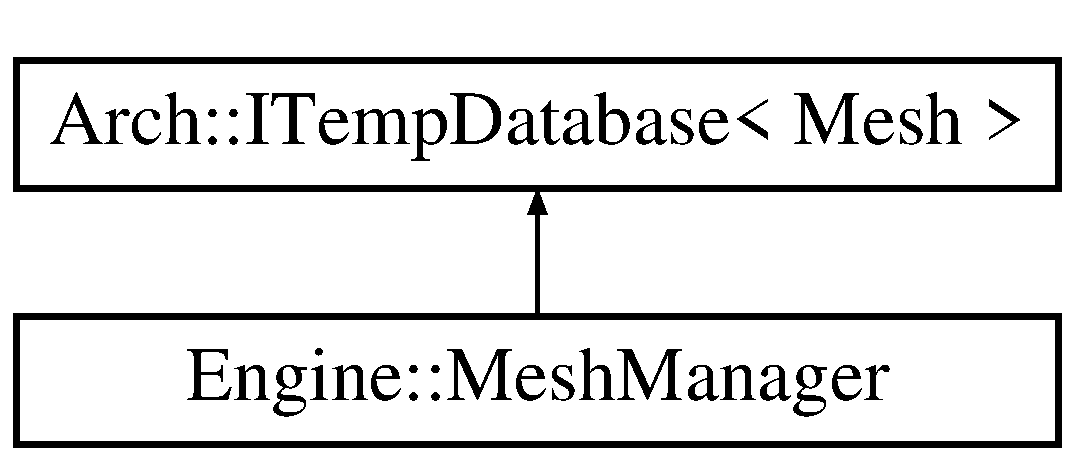
\includegraphics[height=2.000000cm]{classEngine_1_1MeshManager}
\end{center}
\end{figure}
\subsection*{Public Member Functions}
\begin{DoxyCompactItemize}
\item 
\hyperlink{classEngine_1_1GLVertexArrayObject}{G\+L\+Vertex\+Array\+Object} $\ast$ \hyperlink{classEngine_1_1MeshManager_a966a158ba75b202a073992c9a9e27fd0}{create\+Vertex\+Array\+Object} (const \hyperlink{classEngine_1_1MeshData}{Mesh\+Data} \&mesh\+\_\+data)
\begin{DoxyCompactList}\small\item\em create\+Vertex\+Array\+Object \end{DoxyCompactList}\item 
\hyperlink{classEngine_1_1Mesh}{Mesh} $\ast$ \hyperlink{classEngine_1_1MeshManager_a2a5c7a63ef5ecbbb3c754063a7ebc864}{create\+Mesh} (const std\+::string \&resource\+\_\+file)
\begin{DoxyCompactList}\small\item\em create\+Mesh \end{DoxyCompactList}\item 
\hypertarget{classEngine_1_1MeshManager_a05e3a4f93f6a01ced5d5e734ca698e78}{}\hyperlink{classEngine_1_1Mesh}{Mesh} $\ast$ {\bfseries create\+Mesh} (const std\+::string \&resource\+\_\+name, Vector3fv vertices)\label{classEngine_1_1MeshManager_a05e3a4f93f6a01ced5d5e734ca698e78}

\item 
\hypertarget{classEngine_1_1MeshManager_ac030e6b00ec5839d6b7cf01f897078e2}{}\hyperlink{classEngine_1_1Mesh}{Mesh} $\ast$ {\bfseries create\+Embedded\+Mesh} (const std\+::string \&source)\label{classEngine_1_1MeshManager_ac030e6b00ec5839d6b7cf01f897078e2}

\item 
\hyperlink{classEngine_1_1Mesh}{Mesh} $\ast$ \hyperlink{classEngine_1_1MeshManager_a0b273525c26e672a12c660a500f6d776}{get\+Mesh} (uint container\+\_\+id)
\begin{DoxyCompactList}\small\item\em get\+Mesh \end{DoxyCompactList}\item 
void \hyperlink{classEngine_1_1MeshManager_a42a66b67e3123ed190edbd5be5fac412}{destroy} (uint container\+\_\+id)
\begin{DoxyCompactList}\small\item\em destroy \end{DoxyCompactList}\item 
void \hyperlink{classEngine_1_1MeshManager_af9a57216dac74b11f0531058612a1954}{print\+Info\+Message} (const std\+::string \&resource\+\_\+name)
\begin{DoxyCompactList}\small\item\em print\+Info\+Message \end{DoxyCompactList}\end{DoxyCompactItemize}


\subsection{Detailed Description}
The \hyperlink{classEngine_1_1MeshManager}{Mesh\+Manager} class. 

Componentv2 Database ( \hyperlink{classEngine_1_1MeshManager}{Mesh\+Manager} )


\begin{DoxyItemize}
\item create \hyperlink{classEngine_1_1Mesh}{Mesh} Container from file.\+obj
\item create \hyperlink{classEngine_1_1Mesh}{Mesh} Container from \char`\"{}object name\char`\"{} and \char`\"{}vertice list\char`\"{}
\item destroy \hyperlink{classEngine_1_1Mesh}{Mesh} Container 
\end{DoxyItemize}

\subsection{Member Function Documentation}
\hypertarget{classEngine_1_1MeshManager_a2a5c7a63ef5ecbbb3c754063a7ebc864}{}\index{Engine\+::\+Mesh\+Manager@{Engine\+::\+Mesh\+Manager}!create\+Mesh@{create\+Mesh}}
\index{create\+Mesh@{create\+Mesh}!Engine\+::\+Mesh\+Manager@{Engine\+::\+Mesh\+Manager}}
\subsubsection[{create\+Mesh(const std\+::string \&resource\+\_\+file)}]{\setlength{\rightskip}{0pt plus 5cm}{\bf Mesh}$\ast$ Engine\+::\+Mesh\+Manager\+::create\+Mesh (
\begin{DoxyParamCaption}
\item[{const std\+::string \&}]{resource\+\_\+file}
\end{DoxyParamCaption}
)}\label{classEngine_1_1MeshManager_a2a5c7a63ef5ecbbb3c754063a7ebc864}


create\+Mesh 

Create New \hyperlink{classEngine_1_1Mesh}{Mesh} from resource\+\_\+file (aka. obj file ) 
\begin{DoxyParams}{Parameters}
{\em resource\+\_\+file} & \\
\hline
\end{DoxyParams}
\begin{DoxyReturn}{Returns}

\end{DoxyReturn}
\hypertarget{classEngine_1_1MeshManager_a966a158ba75b202a073992c9a9e27fd0}{}\index{Engine\+::\+Mesh\+Manager@{Engine\+::\+Mesh\+Manager}!create\+Vertex\+Array\+Object@{create\+Vertex\+Array\+Object}}
\index{create\+Vertex\+Array\+Object@{create\+Vertex\+Array\+Object}!Engine\+::\+Mesh\+Manager@{Engine\+::\+Mesh\+Manager}}
\subsubsection[{create\+Vertex\+Array\+Object(const Mesh\+Data \&mesh\+\_\+data)}]{\setlength{\rightskip}{0pt plus 5cm}{\bf G\+L\+Vertex\+Array\+Object} $\ast$ Mesh\+Manager\+::create\+Vertex\+Array\+Object (
\begin{DoxyParamCaption}
\item[{const {\bf Mesh\+Data} \&}]{mesh\+\_\+data}
\end{DoxyParamCaption}
)}\label{classEngine_1_1MeshManager_a966a158ba75b202a073992c9a9e27fd0}


create\+Vertex\+Array\+Object 

Create G\+L Buffers 
\begin{DoxyParams}{Parameters}
{\em mesh\+\_\+data} & \\
\hline
\end{DoxyParams}
\begin{DoxyReturn}{Returns}

\end{DoxyReturn}
\hypertarget{classEngine_1_1MeshManager_a42a66b67e3123ed190edbd5be5fac412}{}\index{Engine\+::\+Mesh\+Manager@{Engine\+::\+Mesh\+Manager}!destroy@{destroy}}
\index{destroy@{destroy}!Engine\+::\+Mesh\+Manager@{Engine\+::\+Mesh\+Manager}}
\subsubsection[{destroy(uint container\+\_\+id)}]{\setlength{\rightskip}{0pt plus 5cm}void Mesh\+Manager\+::destroy (
\begin{DoxyParamCaption}
\item[{uint}]{container\+\_\+id}
\end{DoxyParamCaption}
)}\label{classEngine_1_1MeshManager_a42a66b67e3123ed190edbd5be5fac412}


destroy 

Destroy a \hyperlink{classEngine_1_1Mesh}{Mesh} Ptr 
\begin{DoxyParams}{Parameters}
{\em container\+\_\+id} & \\
\hline
\end{DoxyParams}
\hypertarget{classEngine_1_1MeshManager_a0b273525c26e672a12c660a500f6d776}{}\index{Engine\+::\+Mesh\+Manager@{Engine\+::\+Mesh\+Manager}!get\+Mesh@{get\+Mesh}}
\index{get\+Mesh@{get\+Mesh}!Engine\+::\+Mesh\+Manager@{Engine\+::\+Mesh\+Manager}}
\subsubsection[{get\+Mesh(uint container\+\_\+id)}]{\setlength{\rightskip}{0pt plus 5cm}{\bf Mesh} $\ast$ Mesh\+Manager\+::get\+Mesh (
\begin{DoxyParamCaption}
\item[{uint}]{container\+\_\+id}
\end{DoxyParamCaption}
)}\label{classEngine_1_1MeshManager_a0b273525c26e672a12c660a500f6d776}


get\+Mesh 

Return \hyperlink{classEngine_1_1Mesh}{Mesh} by container\+\_\+id 
\begin{DoxyParams}{Parameters}
{\em container\+\_\+id} & \\
\hline
\end{DoxyParams}
\begin{DoxyReturn}{Returns}
\hyperlink{classEngine_1_1Mesh}{Mesh} Ptr 
\end{DoxyReturn}
\hypertarget{classEngine_1_1MeshManager_af9a57216dac74b11f0531058612a1954}{}\index{Engine\+::\+Mesh\+Manager@{Engine\+::\+Mesh\+Manager}!print\+Info\+Message@{print\+Info\+Message}}
\index{print\+Info\+Message@{print\+Info\+Message}!Engine\+::\+Mesh\+Manager@{Engine\+::\+Mesh\+Manager}}
\subsubsection[{print\+Info\+Message(const std\+::string \&resource\+\_\+name)}]{\setlength{\rightskip}{0pt plus 5cm}void Mesh\+Manager\+::print\+Info\+Message (
\begin{DoxyParamCaption}
\item[{const std\+::string \&}]{resource\+\_\+name}
\end{DoxyParamCaption}
)}\label{classEngine_1_1MeshManager_af9a57216dac74b11f0531058612a1954}


print\+Info\+Message 

Print a Info Message 
\begin{DoxyParams}{Parameters}
{\em resource\+\_\+name} & \\
\hline
\end{DoxyParams}


The documentation for this class was generated from the following files\+:\begin{DoxyCompactItemize}
\item 
include/\+Manager/meshmanager.\+h\item 
Engine/\+Manager/Mesh\+Manager.\+cpp\end{DoxyCompactItemize}

\hypertarget{classEngine_1_1MouseEvent}{}\section{Engine\+:\+:Mouse\+Event Class Reference}
\label{classEngine_1_1MouseEvent}\index{Engine\+::\+Mouse\+Event@{Engine\+::\+Mouse\+Event}}


The \hyperlink{classEngine_1_1MouseEvent}{Mouse\+Event} -\/ Event class.  




{\ttfamily \#include $<$input.\+h$>$}

\subsection*{Public Member Functions}
\begin{DoxyCompactItemize}
\item 
\hypertarget{classEngine_1_1MouseEvent_aa89c5787692146a78c7452cec6d5def3}{}int {\bfseries get\+Button} (void) const \label{classEngine_1_1MouseEvent_aa89c5787692146a78c7452cec6d5def3}

\item 
\hypertarget{classEngine_1_1MouseEvent_a3c5c3c0da4eb44c2b8c01c3cbdca3045}{}bool {\bfseries is\+Mouse\+Pressed} (void) const \label{classEngine_1_1MouseEvent_a3c5c3c0da4eb44c2b8c01c3cbdca3045}

\item 
\hypertarget{classEngine_1_1MouseEvent_a023008311538aa982f6c73e0b44e7896}{}bool {\bfseries is\+Mouse\+Released} (void) const \label{classEngine_1_1MouseEvent_a023008311538aa982f6c73e0b44e7896}

\item 
\hypertarget{classEngine_1_1MouseEvent_af3f7da6e5669af6c789e91f19ddf20a7}{}bool {\bfseries is\+Shift\+Down} (void) const \label{classEngine_1_1MouseEvent_af3f7da6e5669af6c789e91f19ddf20a7}

\item 
\hypertarget{classEngine_1_1MouseEvent_aad60b23c3b0041ba2fb0b2c7d6e14ce8}{}bool {\bfseries is\+Control\+Down} (void) const \label{classEngine_1_1MouseEvent_aad60b23c3b0041ba2fb0b2c7d6e14ce8}

\item 
\hypertarget{classEngine_1_1MouseEvent_a78faf293d12284ef5781ea2d51c2d4ed}{}bool {\bfseries is\+Alt\+Down} (void) const \label{classEngine_1_1MouseEvent_a78faf293d12284ef5781ea2d51c2d4ed}

\item 
\hypertarget{classEngine_1_1MouseEvent_af3e6ddbac210840fd2f8be68d95e0bdc}{}bool {\bfseries is\+Super\+Down} (void) const \label{classEngine_1_1MouseEvent_af3e6ddbac210840fd2f8be68d95e0bdc}

\item 
\hypertarget{classEngine_1_1MouseEvent_ad554b256e40f0bd4b7916812e52e17d8}{}int {\bfseries get\+Action} (void) const \label{classEngine_1_1MouseEvent_ad554b256e40f0bd4b7916812e52e17d8}

\item 
\hypertarget{classEngine_1_1MouseEvent_a583266eb9e5d5edce1c878f7c5f3c95c}{}int {\bfseries get\+Mod} (void) const \label{classEngine_1_1MouseEvent_a583266eb9e5d5edce1c878f7c5f3c95c}

\item 
\hypertarget{classEngine_1_1MouseEvent_a49b18f49460d7a398291798478753c42}{}void {\bfseries set\+Action} (int action)\label{classEngine_1_1MouseEvent_a49b18f49460d7a398291798478753c42}

\item 
\hypertarget{classEngine_1_1MouseEvent_a0cee4b15ce7f60e2f85dfc5140efd2c0}{}void {\bfseries set\+Mod} (int mod)\label{classEngine_1_1MouseEvent_a0cee4b15ce7f60e2f85dfc5140efd2c0}

\item 
\hypertarget{classEngine_1_1MouseEvent_a1783ed646cf5a2b9c0984bfce3a8cc89}{}void {\bfseries set\+Button} (int button)\label{classEngine_1_1MouseEvent_a1783ed646cf5a2b9c0984bfce3a8cc89}

\item 
\hypertarget{classEngine_1_1MouseEvent_a4f06d2de67e734d62c6b3f9ee2d3396d}{}void {\bfseries set\+Position} (const \hyperlink{classVector2}{Vector2f} \&vector)\label{classEngine_1_1MouseEvent_a4f06d2de67e734d62c6b3f9ee2d3396d}

\end{DoxyCompactItemize}


\subsection{Detailed Description}
The \hyperlink{classEngine_1_1MouseEvent}{Mouse\+Event} -\/ Event class. 

\hyperlink{classEngine_1_1MouseEvent}{Mouse\+Event} -\/ Store Mouse Data 

The documentation for this class was generated from the following files\+:\begin{DoxyCompactItemize}
\item 
include/\+Container/input.\+h\item 
Container/Mouse\+Event.\+cpp\end{DoxyCompactItemize}

\hypertarget{classEngine_1_1MultiRendering}{}\section{Engine\+:\+:Multi\+Rendering Class Reference}
\label{classEngine_1_1MultiRendering}\index{Engine\+::\+Multi\+Rendering@{Engine\+::\+Multi\+Rendering}}


The \hyperlink{classEngine_1_1MultiRendering}{Multi\+Rendering} -\/ Render System class.  




{\ttfamily \#include $<$multirendering.\+h$>$}

Inheritance diagram for Engine\+:\+:Multi\+Rendering\+:\begin{figure}[H]
\begin{center}
\leavevmode
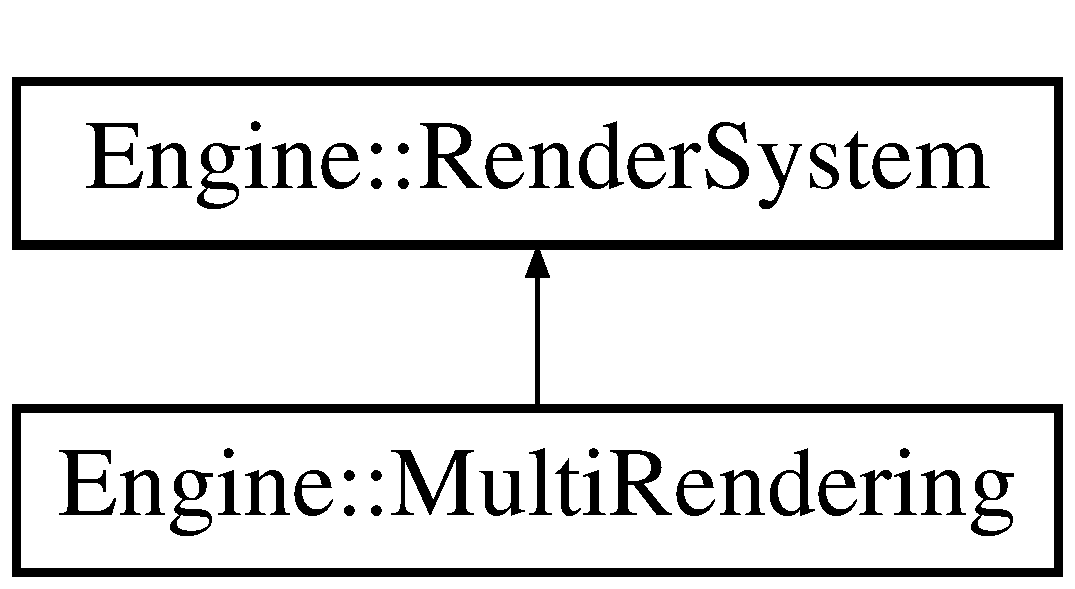
\includegraphics[height=2.000000cm]{classEngine_1_1MultiRendering}
\end{center}
\end{figure}
\subsection*{Public Member Functions}
\begin{DoxyCompactItemize}
\item 
\hypertarget{classEngine_1_1MultiRendering_a2424052bf0bcf131bb1105d00ae160ca}{}{\bfseries Multi\+Rendering} (const std\+::string \&system\+\_\+name)\label{classEngine_1_1MultiRendering_a2424052bf0bcf131bb1105d00ae160ca}

\item 
\hypertarget{classEngine_1_1MultiRendering_a0f36b2037a8d739d0317c2428ef8680d}{}void {\bfseries initialize} (\hyperlink{classEngine_1_1OpenPolygonDisplay}{Open\+Polygon\+Display} $\ast$display) final override\label{classEngine_1_1MultiRendering_a0f36b2037a8d739d0317c2428ef8680d}

\item 
\hypertarget{classEngine_1_1MultiRendering_a664270e53edf1012f5def567222dbd2d}{}void {\bfseries Render\+Frame} (void) final override\label{classEngine_1_1MultiRendering_a664270e53edf1012f5def567222dbd2d}

\item 
\hypertarget{classEngine_1_1MultiRendering_a417089c3206f1c2caa17f818a178496c}{}void {\bfseries Resize} (void) final override\label{classEngine_1_1MultiRendering_a417089c3206f1c2caa17f818a178496c}

\item 
\hypertarget{classEngine_1_1MultiRendering_a8bb0c88c459ae5b3c1e0db8b61e34e9e}{}\hyperlink{classEngine_1_1Position}{Position} $\ast$ {\bfseries get\+Screen\+Position} (void)\label{classEngine_1_1MultiRendering_a8bb0c88c459ae5b3c1e0db8b61e34e9e}

\item 
\hypertarget{classEngine_1_1MultiRendering_a0df4ce83eb604a195ac4cdfe7ac85051}{}\hyperlink{classEngine_1_1Mesh}{Mesh} $\ast$ {\bfseries get\+Screen} (void)\label{classEngine_1_1MultiRendering_a0df4ce83eb604a195ac4cdfe7ac85051}

\end{DoxyCompactItemize}
\subsection*{Additional Inherited Members}


\subsection{Detailed Description}
The \hyperlink{classEngine_1_1MultiRendering}{Multi\+Rendering} -\/ Render System class. 

The documentation for this class was generated from the following files\+:\begin{DoxyCompactItemize}
\item 
include/\+Render/multirendering.\+h\item 
Engine/\+Render/Multi\+Rendering.\+cpp\end{DoxyCompactItemize}

\hypertarget{classEngine_1_1Mutex}{}\section{Engine\+:\+:Mutex Class Reference}
\label{classEngine_1_1Mutex}\index{Engine\+::\+Mutex@{Engine\+::\+Mutex}}
\subsection*{Static Public Member Functions}
\begin{DoxyCompactItemize}
\item 
\hypertarget{classEngine_1_1Mutex_a727a44670b7661702a4562b2111ccc7e}{}static void {\bfseries Sync\+Lock} (void)\label{classEngine_1_1Mutex_a727a44670b7661702a4562b2111ccc7e}

\item 
\hypertarget{classEngine_1_1Mutex_a5cfce9311571230a1b7c2a7898290ddb}{}static void {\bfseries Sync\+Unlock} (void)\label{classEngine_1_1Mutex_a5cfce9311571230a1b7c2a7898290ddb}

\item 
\hypertarget{classEngine_1_1Mutex_a39b1245e69be06a3cffd06d4a4292ea3}{}static void {\bfseries Close\+Lock} (void)\label{classEngine_1_1Mutex_a39b1245e69be06a3cffd06d4a4292ea3}

\item 
\hypertarget{classEngine_1_1Mutex_adc66608d2e6e3b08aaba622f94eb88ce}{}static void {\bfseries Close\+Unlock} (void)\label{classEngine_1_1Mutex_adc66608d2e6e3b08aaba622f94eb88ce}

\end{DoxyCompactItemize}


The documentation for this class was generated from the following files\+:\begin{DoxyCompactItemize}
\item 
include/eutils.\+h\item 
Engine/\+Utils/Utils.\+cpp\end{DoxyCompactItemize}

\hypertarget{classEngine_1_1NodeAnim}{}\section{Engine\+:\+:Node\+Anim Class Reference}
\label{classEngine_1_1NodeAnim}\index{Engine\+::\+Node\+Anim@{Engine\+::\+Node\+Anim}}


The \hyperlink{classEngine_1_1NodeAnim}{Node\+Anim} class.  




{\ttfamily \#include $<$nodeanim.\+h$>$}

\subsection*{Public Member Functions}
\begin{DoxyCompactItemize}
\item 
\hypertarget{classEngine_1_1NodeAnim_a8cfaab7c17ad0c7212904838e8730e5b}{}{\bfseries Node\+Anim} (const std\+::string \&node\+\_\+name)\label{classEngine_1_1NodeAnim_a8cfaab7c17ad0c7212904838e8730e5b}

\item 
void \hyperlink{classEngine_1_1NodeAnim_a02d79743ef4d9d737a2f290b78d765f8}{set\+Rotations} (Vector3fv rotations)
\begin{DoxyCompactList}\small\item\em set\+Rotations \end{DoxyCompactList}\item 
void \hyperlink{classEngine_1_1NodeAnim_a064b09fb930a538fb036fef21ff2f664}{set\+Quanternions} (Vector4fv quats)
\begin{DoxyCompactList}\small\item\em set\+Quanternions \end{DoxyCompactList}\item 
void \hyperlink{classEngine_1_1NodeAnim_a3dfddcefed0d6a2b11349ae5ea23b64f}{set\+Position} (const \hyperlink{classVector3}{Vector3f} \&position)
\begin{DoxyCompactList}\small\item\em set\+Position \end{DoxyCompactList}\item 
void \hyperlink{classEngine_1_1NodeAnim_acdf7bba9515196eec89dca3b3555d13c}{set\+Node\+Name} (const std\+::string \&node\+\_\+name)
\begin{DoxyCompactList}\small\item\em set\+Node\+Name \end{DoxyCompactList}\item 
void \hyperlink{classEngine_1_1NodeAnim_a9a1a94bf9e53180a3810f90685998688}{set\+Node} (\hyperlink{classEngine_1_1NodeAnim}{Node\+Anim} $\ast$node)
\begin{DoxyCompactList}\small\item\em set\+Node \end{DoxyCompactList}\item 
void \hyperlink{classEngine_1_1NodeAnim_aa9fb2456baafae8281c6ea64a45f1176}{add\+Quanternion} (const \hyperlink{classVector4}{Vector4f} \&quat)
\begin{DoxyCompactList}\small\item\em add\+Quanternion \end{DoxyCompactList}\item 
void \hyperlink{classEngine_1_1NodeAnim_ab2ca08d0111650591bd5ddbf0244e460}{add\+Rotation} (const \hyperlink{classVector3}{Vector3f} \&rotation)
\begin{DoxyCompactList}\small\item\em add\+Rotation \end{DoxyCompactList}\item 
const Vector4fv \hyperlink{classEngine_1_1NodeAnim_a5271f3a9ae728cff69911c15b2697ed5}{get\+Quanternions} (void) const 
\begin{DoxyCompactList}\small\item\em get\+Quanternions \end{DoxyCompactList}\item 
const Vector3fv \hyperlink{classEngine_1_1NodeAnim_a92a5f6cb255cf632cfec5f503d5a15d2}{get\+Rotations} (void) const 
\begin{DoxyCompactList}\small\item\em get\+Rotations \end{DoxyCompactList}\item 
const \hyperlink{classVector3}{Vector3f} \& \hyperlink{classEngine_1_1NodeAnim_a17413937ec2344aec8c5c13306f6bdad}{get\+Position} (void) const 
\begin{DoxyCompactList}\small\item\em get\+Position \end{DoxyCompactList}\item 
const std\+::string \& \hyperlink{classEngine_1_1NodeAnim_a8e343fd13892a06a7e894176f37755cd}{get\+Node\+Name} (void) const 
\begin{DoxyCompactList}\small\item\em get\+Node\+Name \end{DoxyCompactList}\item 
\hyperlink{classEngine_1_1NodeAnim}{Node\+Anim} $\ast$ \hyperlink{classEngine_1_1NodeAnim_ab2b8660cf74433045cfbaf9e9c2e8cdc}{get\+Parent\+Node} ()
\begin{DoxyCompactList}\small\item\em get\+Parent\+Node \end{DoxyCompactList}\item 
const \hyperlink{classEngine_1_1NodeAnim}{Node\+Anim} $\ast$ \hyperlink{classEngine_1_1NodeAnim_aee5b3b5484ac623393a8e241c7bf8428}{get\+Const\+Parent\+Node} (void) const 
\begin{DoxyCompactList}\small\item\em get\+Const\+Parent\+Node \end{DoxyCompactList}\item 
void \hyperlink{classEngine_1_1NodeAnim_a71b9b346eb551284dffb86f2dab4a68d}{clear} (void)
\begin{DoxyCompactList}\small\item\em clear \end{DoxyCompactList}\end{DoxyCompactItemize}


\subsection{Detailed Description}
The \hyperlink{classEngine_1_1NodeAnim}{Node\+Anim} class. 

Save Node Data ( aka. \hyperlink{classEngine_1_1Bone}{Bone} Data )
\begin{DoxyItemize}
\item only for custom Loader 
\end{DoxyItemize}

\subsection{Member Function Documentation}
\hypertarget{classEngine_1_1NodeAnim_aa9fb2456baafae8281c6ea64a45f1176}{}\index{Engine\+::\+Node\+Anim@{Engine\+::\+Node\+Anim}!add\+Quanternion@{add\+Quanternion}}
\index{add\+Quanternion@{add\+Quanternion}!Engine\+::\+Node\+Anim@{Engine\+::\+Node\+Anim}}
\subsubsection[{add\+Quanternion(const Vector4f \&quat)}]{\setlength{\rightskip}{0pt plus 5cm}void Node\+Anim\+::add\+Quanternion (
\begin{DoxyParamCaption}
\item[{const {\bf Vector4f} \&}]{quat}
\end{DoxyParamCaption}
)}\label{classEngine_1_1NodeAnim_aa9fb2456baafae8281c6ea64a45f1176}


add\+Quanternion 

Add a Quanternion 
\begin{DoxyParams}{Parameters}
{\em quat} & \\
\hline
\end{DoxyParams}
\hypertarget{classEngine_1_1NodeAnim_ab2ca08d0111650591bd5ddbf0244e460}{}\index{Engine\+::\+Node\+Anim@{Engine\+::\+Node\+Anim}!add\+Rotation@{add\+Rotation}}
\index{add\+Rotation@{add\+Rotation}!Engine\+::\+Node\+Anim@{Engine\+::\+Node\+Anim}}
\subsubsection[{add\+Rotation(const Vector3f \&rotation)}]{\setlength{\rightskip}{0pt plus 5cm}void Node\+Anim\+::add\+Rotation (
\begin{DoxyParamCaption}
\item[{const {\bf Vector3f} \&}]{rotation}
\end{DoxyParamCaption}
)}\label{classEngine_1_1NodeAnim_ab2ca08d0111650591bd5ddbf0244e460}


add\+Rotation 

Add Rotation 
\begin{DoxyParams}{Parameters}
{\em rotation} & \\
\hline
\end{DoxyParams}
\hypertarget{classEngine_1_1NodeAnim_a71b9b346eb551284dffb86f2dab4a68d}{}\index{Engine\+::\+Node\+Anim@{Engine\+::\+Node\+Anim}!clear@{clear}}
\index{clear@{clear}!Engine\+::\+Node\+Anim@{Engine\+::\+Node\+Anim}}
\subsubsection[{clear(void)}]{\setlength{\rightskip}{0pt plus 5cm}void Node\+Anim\+::clear (
\begin{DoxyParamCaption}
\item[{void}]{}
\end{DoxyParamCaption}
)}\label{classEngine_1_1NodeAnim_a71b9b346eb551284dffb86f2dab4a68d}


clear 

clear lists \hypertarget{classEngine_1_1NodeAnim_aee5b3b5484ac623393a8e241c7bf8428}{}\index{Engine\+::\+Node\+Anim@{Engine\+::\+Node\+Anim}!get\+Const\+Parent\+Node@{get\+Const\+Parent\+Node}}
\index{get\+Const\+Parent\+Node@{get\+Const\+Parent\+Node}!Engine\+::\+Node\+Anim@{Engine\+::\+Node\+Anim}}
\subsubsection[{get\+Const\+Parent\+Node(void) const }]{\setlength{\rightskip}{0pt plus 5cm}const {\bf Node\+Anim} $\ast$ Node\+Anim\+::get\+Const\+Parent\+Node (
\begin{DoxyParamCaption}
\item[{void}]{}
\end{DoxyParamCaption}
) const}\label{classEngine_1_1NodeAnim_aee5b3b5484ac623393a8e241c7bf8428}


get\+Const\+Parent\+Node 

\begin{DoxyReturn}{Returns}

\end{DoxyReturn}
\hypertarget{classEngine_1_1NodeAnim_a8e343fd13892a06a7e894176f37755cd}{}\index{Engine\+::\+Node\+Anim@{Engine\+::\+Node\+Anim}!get\+Node\+Name@{get\+Node\+Name}}
\index{get\+Node\+Name@{get\+Node\+Name}!Engine\+::\+Node\+Anim@{Engine\+::\+Node\+Anim}}
\subsubsection[{get\+Node\+Name(void) const }]{\setlength{\rightskip}{0pt plus 5cm}const std\+::string \& Node\+Anim\+::get\+Node\+Name (
\begin{DoxyParamCaption}
\item[{void}]{}
\end{DoxyParamCaption}
) const}\label{classEngine_1_1NodeAnim_a8e343fd13892a06a7e894176f37755cd}


get\+Node\+Name 

Return Node Name \begin{DoxyReturn}{Returns}

\end{DoxyReturn}
\hypertarget{classEngine_1_1NodeAnim_ab2b8660cf74433045cfbaf9e9c2e8cdc}{}\index{Engine\+::\+Node\+Anim@{Engine\+::\+Node\+Anim}!get\+Parent\+Node@{get\+Parent\+Node}}
\index{get\+Parent\+Node@{get\+Parent\+Node}!Engine\+::\+Node\+Anim@{Engine\+::\+Node\+Anim}}
\subsubsection[{get\+Parent\+Node()}]{\setlength{\rightskip}{0pt plus 5cm}{\bf Node\+Anim} $\ast$ Node\+Anim\+::get\+Parent\+Node (
\begin{DoxyParamCaption}
\item[{void}]{}
\end{DoxyParamCaption}
)}\label{classEngine_1_1NodeAnim_ab2b8660cf74433045cfbaf9e9c2e8cdc}


get\+Parent\+Node 

Return Parent Node \begin{DoxyReturn}{Returns}

\end{DoxyReturn}
\hypertarget{classEngine_1_1NodeAnim_a17413937ec2344aec8c5c13306f6bdad}{}\index{Engine\+::\+Node\+Anim@{Engine\+::\+Node\+Anim}!get\+Position@{get\+Position}}
\index{get\+Position@{get\+Position}!Engine\+::\+Node\+Anim@{Engine\+::\+Node\+Anim}}
\subsubsection[{get\+Position(void) const }]{\setlength{\rightskip}{0pt plus 5cm}const {\bf Vector3f} \& Node\+Anim\+::get\+Position (
\begin{DoxyParamCaption}
\item[{void}]{}
\end{DoxyParamCaption}
) const}\label{classEngine_1_1NodeAnim_a17413937ec2344aec8c5c13306f6bdad}


get\+Position 

Return Offset \hyperlink{classEngine_1_1Position}{Position} \begin{DoxyReturn}{Returns}

\end{DoxyReturn}
\hypertarget{classEngine_1_1NodeAnim_a5271f3a9ae728cff69911c15b2697ed5}{}\index{Engine\+::\+Node\+Anim@{Engine\+::\+Node\+Anim}!get\+Quanternions@{get\+Quanternions}}
\index{get\+Quanternions@{get\+Quanternions}!Engine\+::\+Node\+Anim@{Engine\+::\+Node\+Anim}}
\subsubsection[{get\+Quanternions(void) const }]{\setlength{\rightskip}{0pt plus 5cm}const Vector4fv Node\+Anim\+::get\+Quanternions (
\begin{DoxyParamCaption}
\item[{void}]{}
\end{DoxyParamCaption}
) const}\label{classEngine_1_1NodeAnim_a5271f3a9ae728cff69911c15b2697ed5}


get\+Quanternions 

Return Quanternion Array \begin{DoxyReturn}{Returns}

\end{DoxyReturn}
\hypertarget{classEngine_1_1NodeAnim_a92a5f6cb255cf632cfec5f503d5a15d2}{}\index{Engine\+::\+Node\+Anim@{Engine\+::\+Node\+Anim}!get\+Rotations@{get\+Rotations}}
\index{get\+Rotations@{get\+Rotations}!Engine\+::\+Node\+Anim@{Engine\+::\+Node\+Anim}}
\subsubsection[{get\+Rotations(void) const }]{\setlength{\rightskip}{0pt plus 5cm}const Vector3fv Node\+Anim\+::get\+Rotations (
\begin{DoxyParamCaption}
\item[{void}]{}
\end{DoxyParamCaption}
) const}\label{classEngine_1_1NodeAnim_a92a5f6cb255cf632cfec5f503d5a15d2}


get\+Rotations 

Return Rotations \begin{DoxyReturn}{Returns}

\end{DoxyReturn}
\hypertarget{classEngine_1_1NodeAnim_a9a1a94bf9e53180a3810f90685998688}{}\index{Engine\+::\+Node\+Anim@{Engine\+::\+Node\+Anim}!set\+Node@{set\+Node}}
\index{set\+Node@{set\+Node}!Engine\+::\+Node\+Anim@{Engine\+::\+Node\+Anim}}
\subsubsection[{set\+Node(\+Node\+Anim $\ast$node)}]{\setlength{\rightskip}{0pt plus 5cm}void Node\+Anim\+::set\+Node (
\begin{DoxyParamCaption}
\item[{{\bf Node\+Anim} $\ast$}]{node}
\end{DoxyParamCaption}
)}\label{classEngine_1_1NodeAnim_a9a1a94bf9e53180a3810f90685998688}


set\+Node 

set parent node 
\begin{DoxyParams}{Parameters}
{\em node} & \+: parent bone \\
\hline
\end{DoxyParams}
\hypertarget{classEngine_1_1NodeAnim_acdf7bba9515196eec89dca3b3555d13c}{}\index{Engine\+::\+Node\+Anim@{Engine\+::\+Node\+Anim}!set\+Node\+Name@{set\+Node\+Name}}
\index{set\+Node\+Name@{set\+Node\+Name}!Engine\+::\+Node\+Anim@{Engine\+::\+Node\+Anim}}
\subsubsection[{set\+Node\+Name(const std\+::string \&node\+\_\+name)}]{\setlength{\rightskip}{0pt plus 5cm}void Node\+Anim\+::set\+Node\+Name (
\begin{DoxyParamCaption}
\item[{const std\+::string \&}]{node\+\_\+name}
\end{DoxyParamCaption}
)}\label{classEngine_1_1NodeAnim_acdf7bba9515196eec89dca3b3555d13c}


set\+Node\+Name 

set node name 
\begin{DoxyParams}{Parameters}
{\em node\+\_\+name} & \+: node name or bone name \\
\hline
\end{DoxyParams}
\hypertarget{classEngine_1_1NodeAnim_a3dfddcefed0d6a2b11349ae5ea23b64f}{}\index{Engine\+::\+Node\+Anim@{Engine\+::\+Node\+Anim}!set\+Position@{set\+Position}}
\index{set\+Position@{set\+Position}!Engine\+::\+Node\+Anim@{Engine\+::\+Node\+Anim}}
\subsubsection[{set\+Position(const Vector3f \&position)}]{\setlength{\rightskip}{0pt plus 5cm}void Node\+Anim\+::set\+Position (
\begin{DoxyParamCaption}
\item[{const {\bf Vector3f} \&}]{position}
\end{DoxyParamCaption}
)}\label{classEngine_1_1NodeAnim_a3dfddcefed0d6a2b11349ae5ea23b64f}


set\+Position 

Set offset position 
\begin{DoxyParams}{Parameters}
{\em position} & \+: offset position or bone position \\
\hline
\end{DoxyParams}
\hypertarget{classEngine_1_1NodeAnim_a064b09fb930a538fb036fef21ff2f664}{}\index{Engine\+::\+Node\+Anim@{Engine\+::\+Node\+Anim}!set\+Quanternions@{set\+Quanternions}}
\index{set\+Quanternions@{set\+Quanternions}!Engine\+::\+Node\+Anim@{Engine\+::\+Node\+Anim}}
\subsubsection[{set\+Quanternions(\+Vector4fv quats)}]{\setlength{\rightskip}{0pt plus 5cm}void Node\+Anim\+::set\+Quanternions (
\begin{DoxyParamCaption}
\item[{Vector4fv}]{quats}
\end{DoxyParamCaption}
)}\label{classEngine_1_1NodeAnim_a064b09fb930a538fb036fef21ff2f664}


set\+Quanternions 

Set Quanternions like a Vector4f( x , y , z , w ) 
\begin{DoxyParams}{Parameters}
{\em quats} & \+: Vector4f array \\
\hline
\end{DoxyParams}
\hypertarget{classEngine_1_1NodeAnim_a02d79743ef4d9d737a2f290b78d765f8}{}\index{Engine\+::\+Node\+Anim@{Engine\+::\+Node\+Anim}!set\+Rotations@{set\+Rotations}}
\index{set\+Rotations@{set\+Rotations}!Engine\+::\+Node\+Anim@{Engine\+::\+Node\+Anim}}
\subsubsection[{set\+Rotations(\+Vector3fv rotations)}]{\setlength{\rightskip}{0pt plus 5cm}void Node\+Anim\+::set\+Rotations (
\begin{DoxyParamCaption}
\item[{Vector3fv}]{rotations}
\end{DoxyParamCaption}
)}\label{classEngine_1_1NodeAnim_a02d79743ef4d9d737a2f290b78d765f8}


set\+Rotations 


\begin{DoxyParams}{Parameters}
{\em rotations} & \\
\hline
\end{DoxyParams}


The documentation for this class was generated from the following files\+:\begin{DoxyCompactItemize}
\item 
include/\+Container/nodeanim.\+h\item 
Container/Node\+Anim.\+cpp\end{DoxyCompactItemize}

\hypertarget{classEngine_1_1NodeAnimScene}{}\section{Engine\+:\+:Node\+Anim\+Scene Class Reference}
\label{classEngine_1_1NodeAnimScene}\index{Engine\+::\+Node\+Anim\+Scene@{Engine\+::\+Node\+Anim\+Scene}}


The \hyperlink{classEngine_1_1NodeAnimScene}{Node\+Anim\+Scene} class.  




{\ttfamily \#include $<$nodeanimscene.\+h$>$}

\subsection*{Public Member Functions}
\begin{DoxyCompactItemize}
\item 
void \hyperlink{classEngine_1_1NodeAnimScene_ab40c73ecf505129e8cfaf65a5fa7968a}{add\+Node} (\hyperlink{classEngine_1_1NodeAnim}{Node\+Anim} $\ast$node)
\begin{DoxyCompactList}\small\item\em add\+Node \end{DoxyCompactList}\item 
void \hyperlink{classEngine_1_1NodeAnimScene_a26a3ae9cb5c7a42e7fdcf1609b93ad8d}{set\+Max\+Frames} (int frames)
\begin{DoxyCompactList}\small\item\em set\+Max\+Frames \end{DoxyCompactList}\item 
bool \hyperlink{classEngine_1_1NodeAnimScene_a7565e0b231a173e75c1248662dbca9ea}{has\+Nodes} (void) const 
\begin{DoxyCompactList}\small\item\em has\+Nodes \end{DoxyCompactList}\item 
int \hyperlink{classEngine_1_1NodeAnimScene_a4c562c44c4c37479a75ca90e11ac0016}{get\+Num\+Nodes} (void) const 
\begin{DoxyCompactList}\small\item\em get\+Num\+Nodes \end{DoxyCompactList}\item 
int \hyperlink{classEngine_1_1NodeAnimScene_aceb00c5d0002f00046cacb33f7ab9b8b}{get\+Num\+Frames} (void) const 
\begin{DoxyCompactList}\small\item\em get\+Num\+Frames \end{DoxyCompactList}\item 
void \hyperlink{classEngine_1_1NodeAnimScene_adaaaafebc0f25f99c99d22ca645f60ee}{clear} (void) const 
\begin{DoxyCompactList}\small\item\em clear \end{DoxyCompactList}\item 
const Node\+Anims \& \hyperlink{classEngine_1_1NodeAnimScene_a2c8116cee4ff059147480056beb681ac}{get\+Const\+Nodes} (void) const 
\begin{DoxyCompactList}\small\item\em get\+Nodes \end{DoxyCompactList}\item 
Node\+Anims \hyperlink{classEngine_1_1NodeAnimScene_a28844fa338a081c44d937a80b6df447f}{get\+Nodes} (void)
\begin{DoxyCompactList}\small\item\em get\+Nodes \end{DoxyCompactList}\end{DoxyCompactItemize}


\subsection{Detailed Description}
The \hyperlink{classEngine_1_1NodeAnimScene}{Node\+Anim\+Scene} class. 

Make a Node\+Scene from Nodes
\begin{DoxyItemize}
\item only for Custom \hyperlink{classEngine_1_1Animation}{Animation} File Loader 
\end{DoxyItemize}

\subsection{Member Function Documentation}
\hypertarget{classEngine_1_1NodeAnimScene_ab40c73ecf505129e8cfaf65a5fa7968a}{}\index{Engine\+::\+Node\+Anim\+Scene@{Engine\+::\+Node\+Anim\+Scene}!add\+Node@{add\+Node}}
\index{add\+Node@{add\+Node}!Engine\+::\+Node\+Anim\+Scene@{Engine\+::\+Node\+Anim\+Scene}}
\subsubsection[{add\+Node(\+Node\+Anim $\ast$node)}]{\setlength{\rightskip}{0pt plus 5cm}void Node\+Anim\+Scene\+::add\+Node (
\begin{DoxyParamCaption}
\item[{{\bf Node\+Anim} $\ast$}]{node}
\end{DoxyParamCaption}
)}\label{classEngine_1_1NodeAnimScene_ab40c73ecf505129e8cfaf65a5fa7968a}


add\+Node 

Add Node 
\begin{DoxyParams}{Parameters}
{\em node} & \\
\hline
\end{DoxyParams}
\hypertarget{classEngine_1_1NodeAnimScene_adaaaafebc0f25f99c99d22ca645f60ee}{}\index{Engine\+::\+Node\+Anim\+Scene@{Engine\+::\+Node\+Anim\+Scene}!clear@{clear}}
\index{clear@{clear}!Engine\+::\+Node\+Anim\+Scene@{Engine\+::\+Node\+Anim\+Scene}}
\subsubsection[{clear(void) const }]{\setlength{\rightskip}{0pt plus 5cm}void Node\+Anim\+Scene\+::clear (
\begin{DoxyParamCaption}
\item[{void}]{}
\end{DoxyParamCaption}
) const}\label{classEngine_1_1NodeAnimScene_adaaaafebc0f25f99c99d22ca645f60ee}


clear 

destory all nodeanims \hypertarget{classEngine_1_1NodeAnimScene_a2c8116cee4ff059147480056beb681ac}{}\index{Engine\+::\+Node\+Anim\+Scene@{Engine\+::\+Node\+Anim\+Scene}!get\+Const\+Nodes@{get\+Const\+Nodes}}
\index{get\+Const\+Nodes@{get\+Const\+Nodes}!Engine\+::\+Node\+Anim\+Scene@{Engine\+::\+Node\+Anim\+Scene}}
\subsubsection[{get\+Const\+Nodes(void) const }]{\setlength{\rightskip}{0pt plus 5cm}const Node\+Anims \& Node\+Anim\+Scene\+::get\+Const\+Nodes (
\begin{DoxyParamCaption}
\item[{void}]{}
\end{DoxyParamCaption}
) const}\label{classEngine_1_1NodeAnimScene_a2c8116cee4ff059147480056beb681ac}


get\+Nodes 

Return const Nodes \begin{DoxyReturn}{Returns}

\end{DoxyReturn}
\hypertarget{classEngine_1_1NodeAnimScene_a28844fa338a081c44d937a80b6df447f}{}\index{Engine\+::\+Node\+Anim\+Scene@{Engine\+::\+Node\+Anim\+Scene}!get\+Nodes@{get\+Nodes}}
\index{get\+Nodes@{get\+Nodes}!Engine\+::\+Node\+Anim\+Scene@{Engine\+::\+Node\+Anim\+Scene}}
\subsubsection[{get\+Nodes(void)}]{\setlength{\rightskip}{0pt plus 5cm}Node\+Anims Node\+Anim\+Scene\+::get\+Nodes (
\begin{DoxyParamCaption}
\item[{void}]{}
\end{DoxyParamCaption}
)}\label{classEngine_1_1NodeAnimScene_a28844fa338a081c44d937a80b6df447f}


get\+Nodes 

Return Nodes \begin{DoxyReturn}{Returns}

\end{DoxyReturn}
\hypertarget{classEngine_1_1NodeAnimScene_aceb00c5d0002f00046cacb33f7ab9b8b}{}\index{Engine\+::\+Node\+Anim\+Scene@{Engine\+::\+Node\+Anim\+Scene}!get\+Num\+Frames@{get\+Num\+Frames}}
\index{get\+Num\+Frames@{get\+Num\+Frames}!Engine\+::\+Node\+Anim\+Scene@{Engine\+::\+Node\+Anim\+Scene}}
\subsubsection[{get\+Num\+Frames(void) const }]{\setlength{\rightskip}{0pt plus 5cm}int Node\+Anim\+Scene\+::get\+Num\+Frames (
\begin{DoxyParamCaption}
\item[{void}]{}
\end{DoxyParamCaption}
) const}\label{classEngine_1_1NodeAnimScene_aceb00c5d0002f00046cacb33f7ab9b8b}


get\+Num\+Frames 

Return amount of frames \begin{DoxyReturn}{Returns}

\end{DoxyReturn}
\hypertarget{classEngine_1_1NodeAnimScene_a4c562c44c4c37479a75ca90e11ac0016}{}\index{Engine\+::\+Node\+Anim\+Scene@{Engine\+::\+Node\+Anim\+Scene}!get\+Num\+Nodes@{get\+Num\+Nodes}}
\index{get\+Num\+Nodes@{get\+Num\+Nodes}!Engine\+::\+Node\+Anim\+Scene@{Engine\+::\+Node\+Anim\+Scene}}
\subsubsection[{get\+Num\+Nodes(void) const }]{\setlength{\rightskip}{0pt plus 5cm}int Node\+Anim\+Scene\+::get\+Num\+Nodes (
\begin{DoxyParamCaption}
\item[{void}]{}
\end{DoxyParamCaption}
) const}\label{classEngine_1_1NodeAnimScene_a4c562c44c4c37479a75ca90e11ac0016}


get\+Num\+Nodes 

Return amount of nodes \begin{DoxyReturn}{Returns}

\end{DoxyReturn}
\hypertarget{classEngine_1_1NodeAnimScene_a7565e0b231a173e75c1248662dbca9ea}{}\index{Engine\+::\+Node\+Anim\+Scene@{Engine\+::\+Node\+Anim\+Scene}!has\+Nodes@{has\+Nodes}}
\index{has\+Nodes@{has\+Nodes}!Engine\+::\+Node\+Anim\+Scene@{Engine\+::\+Node\+Anim\+Scene}}
\subsubsection[{has\+Nodes(void) const }]{\setlength{\rightskip}{0pt plus 5cm}bool Node\+Anim\+Scene\+::has\+Nodes (
\begin{DoxyParamCaption}
\item[{void}]{}
\end{DoxyParamCaption}
) const}\label{classEngine_1_1NodeAnimScene_a7565e0b231a173e75c1248662dbca9ea}


has\+Nodes 

has nodes then return true otherwise false \begin{DoxyReturn}{Returns}

\end{DoxyReturn}
\hypertarget{classEngine_1_1NodeAnimScene_a26a3ae9cb5c7a42e7fdcf1609b93ad8d}{}\index{Engine\+::\+Node\+Anim\+Scene@{Engine\+::\+Node\+Anim\+Scene}!set\+Max\+Frames@{set\+Max\+Frames}}
\index{set\+Max\+Frames@{set\+Max\+Frames}!Engine\+::\+Node\+Anim\+Scene@{Engine\+::\+Node\+Anim\+Scene}}
\subsubsection[{set\+Max\+Frames(int frames)}]{\setlength{\rightskip}{0pt plus 5cm}void Node\+Anim\+Scene\+::set\+Max\+Frames (
\begin{DoxyParamCaption}
\item[{int}]{frames}
\end{DoxyParamCaption}
)}\label{classEngine_1_1NodeAnimScene_a26a3ae9cb5c7a42e7fdcf1609b93ad8d}


set\+Max\+Frames 

set max frames 
\begin{DoxyParams}{Parameters}
{\em frames} & \\
\hline
\end{DoxyParams}


The documentation for this class was generated from the following files\+:\begin{DoxyCompactItemize}
\item 
include/\+Container/nodeanimscene.\+h\item 
Container/Node\+Anim\+Scene.\+cpp\end{DoxyCompactItemize}

\hypertarget{structEngine_1_1ObjectBox}{}\section{Engine\+:\+:Object\+Box Struct Reference}
\label{structEngine_1_1ObjectBox}\index{Engine\+::\+Object\+Box@{Engine\+::\+Object\+Box}}
\subsection*{Public Attributes}
\begin{DoxyCompactItemize}
\item 
\hypertarget{structEngine_1_1ObjectBox_ae323909f489e2f65ca11cdc8d54b7e66}{}float {\bfseries x}\label{structEngine_1_1ObjectBox_ae323909f489e2f65ca11cdc8d54b7e66}

\item 
\hypertarget{structEngine_1_1ObjectBox_a625f072b29b3c33d42c9c8a20e325bf2}{}float {\bfseries y}\label{structEngine_1_1ObjectBox_a625f072b29b3c33d42c9c8a20e325bf2}

\item 
\hypertarget{structEngine_1_1ObjectBox_a098cbccee47677bda8356351a7052d92}{}float {\bfseries width}\label{structEngine_1_1ObjectBox_a098cbccee47677bda8356351a7052d92}

\item 
\hypertarget{structEngine_1_1ObjectBox_a572e1eed2456dd5d1e27a35e1174c404}{}float {\bfseries height}\label{structEngine_1_1ObjectBox_a572e1eed2456dd5d1e27a35e1174c404}

\end{DoxyCompactItemize}


The documentation for this struct was generated from the following file\+:\begin{DoxyCompactItemize}
\item 
include/eutils.\+h\end{DoxyCompactItemize}

\hypertarget{classEngine_1_1OpenPolygon}{}\section{Engine\+:\+:Open\+Polygon Class Reference}
\label{classEngine_1_1OpenPolygon}\index{Engine\+::\+Open\+Polygon@{Engine\+::\+Open\+Polygon}}


The \hyperlink{classEngine_1_1OpenPolygon}{Open\+Polygon} -\/ Main class.  




{\ttfamily \#include $<$openpolygon.\+h$>$}

\subsection*{Public Member Functions}
\begin{DoxyCompactItemize}
\item 
\hypertarget{classEngine_1_1OpenPolygon_aad826a86674a3b92d97658ee25ec8f6b}{}D\+E\+P\+R\+E\+C\+A\+T\+E\+D void {\bfseries write\+Config} (const std\+::string \&config\+\_\+file)\label{classEngine_1_1OpenPolygon_aad826a86674a3b92d97658ee25ec8f6b}

\item 
\hypertarget{classEngine_1_1OpenPolygon_a913c5e47d130c6f9960b01db2f31725d}{}D\+E\+P\+R\+E\+C\+A\+T\+E\+D \hyperlink{classEngine_1_1DisplayConfig}{Display\+Config} {\bfseries read\+Config} (const std\+::string \&config\+\_\+file)\label{classEngine_1_1OpenPolygon_a913c5e47d130c6f9960b01db2f31725d}

\item 
\hyperlink{classEngine_1_1GLFWDisplay}{G\+L\+F\+W\+Display} $\ast$ \hyperlink{classEngine_1_1OpenPolygon_adac81701d470c58bbdb3d14c989f1949}{initialize} (\hyperlink{classEngine_1_1DisplayConfig}{Display\+Config} $\ast$config)
\begin{DoxyCompactList}\small\item\em initialize \end{DoxyCompactList}\item 
void \hyperlink{classEngine_1_1OpenPolygon_a9181551ff0eb633b6db245d3463f662d}{Render\+Loop} (\hyperlink{classEngine_1_1GLFWDisplay}{G\+L\+F\+W\+Display} $\ast$display)
\begin{DoxyCompactList}\small\item\em Render\+Loop. \end{DoxyCompactList}\item 
void \hyperlink{classEngine_1_1OpenPolygon_a1c593a74edb697ba54f956b6bde598ed}{finish} (void)
\begin{DoxyCompactList}\small\item\em finish \end{DoxyCompactList}\end{DoxyCompactItemize}


\subsection{Detailed Description}
The \hyperlink{classEngine_1_1OpenPolygon}{Open\+Polygon} -\/ Main class. 

\subsection{Member Function Documentation}
\hypertarget{classEngine_1_1OpenPolygon_a1c593a74edb697ba54f956b6bde598ed}{}\index{Engine\+::\+Open\+Polygon@{Engine\+::\+Open\+Polygon}!finish@{finish}}
\index{finish@{finish}!Engine\+::\+Open\+Polygon@{Engine\+::\+Open\+Polygon}}
\subsubsection[{finish(void)}]{\setlength{\rightskip}{0pt plus 5cm}void Open\+Polygon\+::finish (
\begin{DoxyParamCaption}
\item[{void}]{}
\end{DoxyParamCaption}
)}\label{classEngine_1_1OpenPolygon_a1c593a74edb697ba54f956b6bde598ed}


finish 

Clear Singletons \hypertarget{classEngine_1_1OpenPolygon_adac81701d470c58bbdb3d14c989f1949}{}\index{Engine\+::\+Open\+Polygon@{Engine\+::\+Open\+Polygon}!initialize@{initialize}}
\index{initialize@{initialize}!Engine\+::\+Open\+Polygon@{Engine\+::\+Open\+Polygon}}
\subsubsection[{initialize(\+Display\+Config $\ast$config)}]{\setlength{\rightskip}{0pt plus 5cm}{\bf G\+L\+F\+W\+Display} $\ast$ Open\+Polygon\+::initialize (
\begin{DoxyParamCaption}
\item[{{\bf Display\+Config} $\ast$}]{config}
\end{DoxyParamCaption}
)}\label{classEngine_1_1OpenPolygon_adac81701d470c58bbdb3d14c989f1949}


initialize 

Create Display 
\begin{DoxyParams}{Parameters}
{\em display} & \\
\hline
\end{DoxyParams}
\begin{DoxyReturn}{Returns}

\end{DoxyReturn}
\hypertarget{classEngine_1_1OpenPolygon_a9181551ff0eb633b6db245d3463f662d}{}\index{Engine\+::\+Open\+Polygon@{Engine\+::\+Open\+Polygon}!Render\+Loop@{Render\+Loop}}
\index{Render\+Loop@{Render\+Loop}!Engine\+::\+Open\+Polygon@{Engine\+::\+Open\+Polygon}}
\subsubsection[{Render\+Loop(\+G\+L\+F\+W\+Display $\ast$display)}]{\setlength{\rightskip}{0pt plus 5cm}void Open\+Polygon\+::\+Render\+Loop (
\begin{DoxyParamCaption}
\item[{{\bf G\+L\+F\+W\+Display} $\ast$}]{display}
\end{DoxyParamCaption}
)}\label{classEngine_1_1OpenPolygon_a9181551ff0eb633b6db245d3463f662d}


Render\+Loop. 

Start Rendering with Display 
\begin{DoxyParams}{Parameters}
{\em display} & \\
\hline
\end{DoxyParams}


The documentation for this class was generated from the following files\+:\begin{DoxyCompactItemize}
\item 
include/openpolygon.\+h\item 
Engine/Open\+Polygon.\+cpp\end{DoxyCompactItemize}

\hypertarget{classEngine_1_1OpenPolygonDisplay}{}\section{Engine\+:\+:Open\+Polygon\+Display Class Reference}
\label{classEngine_1_1OpenPolygonDisplay}\index{Engine\+::\+Open\+Polygon\+Display@{Engine\+::\+Open\+Polygon\+Display}}


The \hyperlink{classEngine_1_1OpenPolygonDisplay}{Open\+Polygon\+Display} -\/ display abstract class.  




{\ttfamily \#include $<$display.\+h$>$}

Inheritance diagram for Engine\+:\+:Open\+Polygon\+Display\+:\begin{figure}[H]
\begin{center}
\leavevmode
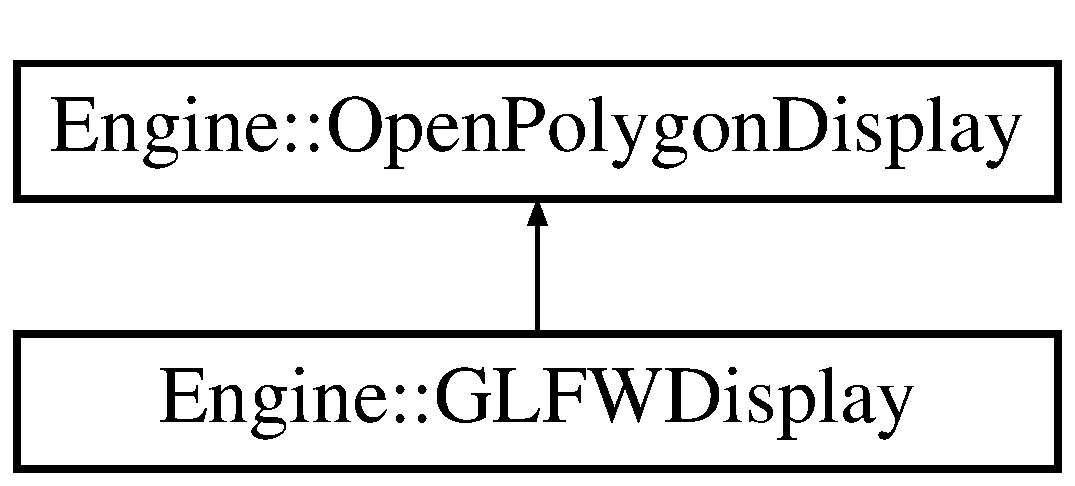
\includegraphics[height=2.000000cm]{classEngine_1_1OpenPolygonDisplay}
\end{center}
\end{figure}
\subsection*{Public Member Functions}
\begin{DoxyCompactItemize}
\item 
\hypertarget{classEngine_1_1OpenPolygonDisplay_a1ba8c36a77b37f480b3f48e59d81b7d2}{}{\bfseries Open\+Polygon\+Display} (const std\+::string \&display\+\_\+name)\label{classEngine_1_1OpenPolygonDisplay_a1ba8c36a77b37f480b3f48e59d81b7d2}

\item 
\hypertarget{classEngine_1_1OpenPolygonDisplay_ae948a2f2522ab508915786e2793cbf99}{}virtual void {\bfseries Close} (void)=0\label{classEngine_1_1OpenPolygonDisplay_ae948a2f2522ab508915786e2793cbf99}

\item 
\hypertarget{classEngine_1_1OpenPolygonDisplay_a5f46947a434abca0ed0013e5b635a950}{}virtual bool {\bfseries is\+Closed} (void)=0\label{classEngine_1_1OpenPolygonDisplay_a5f46947a434abca0ed0013e5b635a950}

\item 
\hypertarget{classEngine_1_1OpenPolygonDisplay_a6d73e3c06fc6ea13b505a4f9d3b075e1}{}virtual void {\bfseries Update} (void)=0\label{classEngine_1_1OpenPolygonDisplay_a6d73e3c06fc6ea13b505a4f9d3b075e1}

\item 
\hypertarget{classEngine_1_1OpenPolygonDisplay_adf1b620cf55e181280bb36d5cd1eda04}{}virtual void {\bfseries set\+Title} (const char $\ast$title)=0\label{classEngine_1_1OpenPolygonDisplay_adf1b620cf55e181280bb36d5cd1eda04}

\item 
\hypertarget{classEngine_1_1OpenPolygonDisplay_aae3bd963682f94241d31d580338f8d0c}{}void {\bfseries set\+Camera} (\hyperlink{classEngine_1_1Camera}{Camera} $\ast$camera)\label{classEngine_1_1OpenPolygonDisplay_aae3bd963682f94241d31d580338f8d0c}

\item 
\hypertarget{classEngine_1_1OpenPolygonDisplay_a8172ae674320280531082c0eb8df5001}{}void {\bfseries set\+View\+Port} (int x, int y, int width, int height)\label{classEngine_1_1OpenPolygonDisplay_a8172ae674320280531082c0eb8df5001}

\item 
\hypertarget{classEngine_1_1OpenPolygonDisplay_a3c4ed33ec18d81d0e5ffe1a4cadb376b}{}void {\bfseries set\+Perspective} (glm\+::mat4 matrix)\label{classEngine_1_1OpenPolygonDisplay_a3c4ed33ec18d81d0e5ffe1a4cadb376b}

\item 
\hypertarget{classEngine_1_1OpenPolygonDisplay_a28c69d28bec97bc043825095d8de13eb}{}void {\bfseries set\+Perspective} (float fovy, float aspect, float near, float far)\label{classEngine_1_1OpenPolygonDisplay_a28c69d28bec97bc043825095d8de13eb}

\item 
\hypertarget{classEngine_1_1OpenPolygonDisplay_ab0487fc26b1ca14425500991502eeb40}{}\hyperlink{classEngine_1_1Camera}{Camera} $\ast$ {\bfseries get\+Camera} (void)\label{classEngine_1_1OpenPolygonDisplay_ab0487fc26b1ca14425500991502eeb40}

\item 
\hypertarget{classEngine_1_1OpenPolygonDisplay_ad6a8931e89242a78ce14a9f2b3056813}{}int {\bfseries get\+Render\+Height} (void)\label{classEngine_1_1OpenPolygonDisplay_ad6a8931e89242a78ce14a9f2b3056813}

\item 
\hypertarget{classEngine_1_1OpenPolygonDisplay_a218d172912b295115b9d59184e4bde91}{}int {\bfseries get\+Render\+Width} (void)\label{classEngine_1_1OpenPolygonDisplay_a218d172912b295115b9d59184e4bde91}

\item 
\hypertarget{classEngine_1_1OpenPolygonDisplay_a0b81459f4aa0397147c3e6431bc68326}{}int {\bfseries get\+View\+Port\+X} (void)\label{classEngine_1_1OpenPolygonDisplay_a0b81459f4aa0397147c3e6431bc68326}

\item 
\hypertarget{classEngine_1_1OpenPolygonDisplay_a416ea86d55883718ede5f1796f5be1c5}{}int {\bfseries get\+View\+Port\+Y} (void)\label{classEngine_1_1OpenPolygonDisplay_a416ea86d55883718ede5f1796f5be1c5}

\item 
\hypertarget{classEngine_1_1OpenPolygonDisplay_af44b37c7fc64d58eb3ee4afc41fabef7}{}const std\+::string \& {\bfseries get\+Name} (void)\label{classEngine_1_1OpenPolygonDisplay_af44b37c7fc64d58eb3ee4afc41fabef7}

\item 
\hypertarget{classEngine_1_1OpenPolygonDisplay_ac66d54b60c7c2ccac4482d2af84ca05b}{}const char $\ast$ {\bfseries get\+Title} (void)\label{classEngine_1_1OpenPolygonDisplay_ac66d54b60c7c2ccac4482d2af84ca05b}

\item 
\hypertarget{classEngine_1_1OpenPolygonDisplay_a1364aa54d94fd6549beac09b03fe13c7}{}glm\+::mat4 {\bfseries get\+Perspective} (void)\label{classEngine_1_1OpenPolygonDisplay_a1364aa54d94fd6549beac09b03fe13c7}

\end{DoxyCompactItemize}
\subsection*{Protected Attributes}
\begin{DoxyCompactItemize}
\item 
\hypertarget{classEngine_1_1OpenPolygonDisplay_a01757c9ac3a6a7154bcbce0554f073d4}{}\hyperlink{classEngine_1_1Camera}{Camera} $\ast$ {\bfseries m\+\_\+camera}\label{classEngine_1_1OpenPolygonDisplay_a01757c9ac3a6a7154bcbce0554f073d4}

\item 
\hypertarget{classEngine_1_1OpenPolygonDisplay_a57815602663a8c4a3614eb1e92753a7e}{}\hyperlink{structEngine_1_1DisplayData}{Display\+Data} {\bfseries m\+\_\+display\+\_\+data}\label{classEngine_1_1OpenPolygonDisplay_a57815602663a8c4a3614eb1e92753a7e}

\end{DoxyCompactItemize}


\subsection{Detailed Description}
The \hyperlink{classEngine_1_1OpenPolygonDisplay}{Open\+Polygon\+Display} -\/ display abstract class. 

The documentation for this class was generated from the following files\+:\begin{DoxyCompactItemize}
\item 
include/\+Container/display.\+h\item 
Container/Display.\+cpp\end{DoxyCompactItemize}

\hypertarget{classEngine_1_1Overlay}{}\section{Engine\+:\+:Overlay Class Reference}
\label{classEngine_1_1Overlay}\index{Engine\+::\+Overlay@{Engine\+::\+Overlay}}


The \hyperlink{classEngine_1_1Overlay}{Overlay} -\/ container class -\/ list of Render\+Elements.  




{\ttfamily \#include $<$overlay.\+h$>$}

\subsection*{Public Member Functions}
\begin{DoxyCompactItemize}
\item 
\hyperlink{classEngine_1_1Overlay_a0d4fec7570e42302be58751898124a54}{Overlay} (const std\+::string \&overlay\+\_\+name)
\begin{DoxyCompactList}\small\item\em \hyperlink{classEngine_1_1Overlay}{Overlay}. \end{DoxyCompactList}\item 
\hypertarget{classEngine_1_1Overlay_a57c16b1fd756a67169ede7623c3a1acf}{}void {\bfseries finish} (void)\label{classEngine_1_1Overlay_a57c16b1fd756a67169ede7623c3a1acf}

\item 
const std\+::string \& \hyperlink{classEngine_1_1Overlay_a2811875f49a01ed373273f05923a967c}{get\+Name} (void) const 
\begin{DoxyCompactList}\small\item\em get\+Name \end{DoxyCompactList}\item 
void \hyperlink{classEngine_1_1Overlay_a543a6ebad7a8e14f9950bb3ce5e2375c}{add\+Element} (\hyperlink{classEngine_1_1RenderElement}{Render\+Element} $\ast$element)
\begin{DoxyCompactList}\small\item\em add\+Element \end{DoxyCompactList}\item 
void \hyperlink{classEngine_1_1Overlay_a65ac966bde65f657f361f080ecb9a6cb}{remove} (\hyperlink{classEngine_1_1RenderElement}{Render\+Element} $\ast$element)
\begin{DoxyCompactList}\small\item\em remove \end{DoxyCompactList}\item 
Elements \hyperlink{classEngine_1_1Overlay_a3b59be62922ee7c3ec7b41a98326802c}{get\+Elements} (void)
\begin{DoxyCompactList}\small\item\em get\+Elements \end{DoxyCompactList}\item 
void \hyperlink{classEngine_1_1Overlay_ae06d70a5d7e885df7bb59996e162a70f}{render} (const \hyperlink{classEngine_1_1DrawEvent}{Draw\+Event} \&event)
\begin{DoxyCompactList}\small\item\em render \end{DoxyCompactList}\item 
\hypertarget{classEngine_1_1Overlay_a494f4baa38d9d044bac190e94e5d0cbb}{}bool {\bfseries is\+Visible} (void)\label{classEngine_1_1Overlay_a494f4baa38d9d044bac190e94e5d0cbb}

\item 
\hypertarget{classEngine_1_1Overlay_ae2826553d74a1884bcdfbcd1a108002c}{}void {\bfseries set\+Visible} (bool status)\label{classEngine_1_1Overlay_ae2826553d74a1884bcdfbcd1a108002c}

\end{DoxyCompactItemize}


\subsection{Detailed Description}
The \hyperlink{classEngine_1_1Overlay}{Overlay} -\/ container class -\/ list of Render\+Elements. 

\subsection{Constructor \& Destructor Documentation}
\hypertarget{classEngine_1_1Overlay_a0d4fec7570e42302be58751898124a54}{}\index{Engine\+::\+Overlay@{Engine\+::\+Overlay}!Overlay@{Overlay}}
\index{Overlay@{Overlay}!Engine\+::\+Overlay@{Engine\+::\+Overlay}}
\subsubsection[{Overlay(const std\+::string \&overlay\+\_\+name)}]{\setlength{\rightskip}{0pt plus 5cm}Overlay\+::\+Overlay (
\begin{DoxyParamCaption}
\item[{const std\+::string \&}]{overlay\+\_\+name}
\end{DoxyParamCaption}
)\hspace{0.3cm}{\ttfamily [explicit]}}\label{classEngine_1_1Overlay_a0d4fec7570e42302be58751898124a54}


\hyperlink{classEngine_1_1Overlay}{Overlay}. 

Create a \hyperlink{classEngine_1_1Overlay}{Overlay} with Name 
\begin{DoxyParams}{Parameters}
{\em overlay\+\_\+name} & \\
\hline
\end{DoxyParams}


\subsection{Member Function Documentation}
\hypertarget{classEngine_1_1Overlay_a543a6ebad7a8e14f9950bb3ce5e2375c}{}\index{Engine\+::\+Overlay@{Engine\+::\+Overlay}!add\+Element@{add\+Element}}
\index{add\+Element@{add\+Element}!Engine\+::\+Overlay@{Engine\+::\+Overlay}}
\subsubsection[{add\+Element(\+Render\+Element $\ast$element)}]{\setlength{\rightskip}{0pt plus 5cm}void Overlay\+::add\+Element (
\begin{DoxyParamCaption}
\item[{{\bf Render\+Element} $\ast$}]{element}
\end{DoxyParamCaption}
)}\label{classEngine_1_1Overlay_a543a6ebad7a8e14f9950bb3ce5e2375c}


add\+Element 

Add a \hyperlink{classEngine_1_1Element}{Element} 
\begin{DoxyParams}{Parameters}
{\em element} & \\
\hline
\end{DoxyParams}
\hypertarget{classEngine_1_1Overlay_a3b59be62922ee7c3ec7b41a98326802c}{}\index{Engine\+::\+Overlay@{Engine\+::\+Overlay}!get\+Elements@{get\+Elements}}
\index{get\+Elements@{get\+Elements}!Engine\+::\+Overlay@{Engine\+::\+Overlay}}
\subsubsection[{get\+Elements(void)}]{\setlength{\rightskip}{0pt plus 5cm}Elements Overlay\+::get\+Elements (
\begin{DoxyParamCaption}
\item[{void}]{}
\end{DoxyParamCaption}
)}\label{classEngine_1_1Overlay_a3b59be62922ee7c3ec7b41a98326802c}


get\+Elements 

Return all Elements \begin{DoxyReturn}{Returns}

\end{DoxyReturn}
\hypertarget{classEngine_1_1Overlay_a2811875f49a01ed373273f05923a967c}{}\index{Engine\+::\+Overlay@{Engine\+::\+Overlay}!get\+Name@{get\+Name}}
\index{get\+Name@{get\+Name}!Engine\+::\+Overlay@{Engine\+::\+Overlay}}
\subsubsection[{get\+Name(void) const }]{\setlength{\rightskip}{0pt plus 5cm}const std\+::string \& Overlay\+::get\+Name (
\begin{DoxyParamCaption}
\item[{void}]{}
\end{DoxyParamCaption}
) const}\label{classEngine_1_1Overlay_a2811875f49a01ed373273f05923a967c}


get\+Name 

Return \hyperlink{classEngine_1_1Overlay}{Overlay} name \begin{DoxyReturn}{Returns}

\end{DoxyReturn}
\hypertarget{classEngine_1_1Overlay_a65ac966bde65f657f361f080ecb9a6cb}{}\index{Engine\+::\+Overlay@{Engine\+::\+Overlay}!remove@{remove}}
\index{remove@{remove}!Engine\+::\+Overlay@{Engine\+::\+Overlay}}
\subsubsection[{remove(\+Render\+Element $\ast$element)}]{\setlength{\rightskip}{0pt plus 5cm}void Overlay\+::remove (
\begin{DoxyParamCaption}
\item[{{\bf Render\+Element} $\ast$}]{element}
\end{DoxyParamCaption}
)}\label{classEngine_1_1Overlay_a65ac966bde65f657f361f080ecb9a6cb}


remove 

Remove a \hyperlink{classEngine_1_1Element}{Element} 
\begin{DoxyParams}{Parameters}
{\em element} & \\
\hline
\end{DoxyParams}
\hypertarget{classEngine_1_1Overlay_ae06d70a5d7e885df7bb59996e162a70f}{}\index{Engine\+::\+Overlay@{Engine\+::\+Overlay}!render@{render}}
\index{render@{render}!Engine\+::\+Overlay@{Engine\+::\+Overlay}}
\subsubsection[{render(const Draw\+Event \&event)}]{\setlength{\rightskip}{0pt plus 5cm}void Overlay\+::render (
\begin{DoxyParamCaption}
\item[{const {\bf Draw\+Event} \&}]{event}
\end{DoxyParamCaption}
)}\label{classEngine_1_1Overlay_ae06d70a5d7e885df7bb59996e162a70f}


render 

Render all \hyperlink{classEngine_1_1Overlay}{Overlay} Elements 

The documentation for this class was generated from the following files\+:\begin{DoxyCompactItemize}
\item 
include/\+Container/overlay.\+h\item 
Container/Overlay.\+cpp\end{DoxyCompactItemize}

\hypertarget{classEngine_1_1OverlayManager}{}\section{Engine\+:\+:Overlay\+Manager Class Reference}
\label{classEngine_1_1OverlayManager}\index{Engine\+::\+Overlay\+Manager@{Engine\+::\+Overlay\+Manager}}


The \hyperlink{classEngine_1_1OverlayManager}{Overlay\+Manager} class.  




{\ttfamily \#include $<$overlaymanager.\+h$>$}

\subsection*{Public Member Functions}
\begin{DoxyCompactItemize}
\item 
\hypertarget{classEngine_1_1OverlayManager_a4031a3daa9c8ecafceaf3b3b842f32fa}{}void {\bfseries finish} (void)\label{classEngine_1_1OverlayManager_a4031a3daa9c8ecafceaf3b3b842f32fa}

\item 
\hyperlink{classEngine_1_1Overlay}{Overlay} $\ast$ \hyperlink{classEngine_1_1OverlayManager_a7bba3a6a67c5d5a6f80486b9775c22b7}{create\+Overlay} (const std\+::string \&overlay\+\_\+name)
\begin{DoxyCompactList}\small\item\em create\+Overlay \end{DoxyCompactList}\item 
\hyperlink{classEngine_1_1Overlay}{Overlay} $\ast$ \hyperlink{classEngine_1_1OverlayManager_afee61b9ea8bb3771231d56b0c0a6817c}{get\+Overlay} (const std\+::string \&overlay\+\_\+name)  throw ( std\+::runtime\+\_\+error)
\begin{DoxyCompactList}\small\item\em get\+Overlay \end{DoxyCompactList}\item 
void \hyperlink{classEngine_1_1OverlayManager_a7e8cca44ab6be17f579b4e06152acb50}{remove\+Overlay} (const std\+::string \&overlay\+\_\+name)  throw ( std\+::runtime\+\_\+error)
\begin{DoxyCompactList}\small\item\em remove\+Overlay \end{DoxyCompactList}\item 
void \hyperlink{classEngine_1_1OverlayManager_a9a4a550f2e053b6909d1642d32f877a8}{remove\+Overlay} (\hyperlink{classEngine_1_1Overlay}{Overlay} $\ast$overlay)
\begin{DoxyCompactList}\small\item\em remove\+Overlay \end{DoxyCompactList}\item 
Overlays \hyperlink{classEngine_1_1OverlayManager_ae46ff201f2f790e3fe0c06b563b54e3e}{get\+Overlays} (void)
\begin{DoxyCompactList}\small\item\em get\+Overlays \end{DoxyCompactList}\end{DoxyCompactItemize}
\subsection*{Static Public Member Functions}
\begin{DoxyCompactItemize}
\item 
static \hyperlink{classEngine_1_1OverlayManager}{Overlay\+Manager} $\ast$ \hyperlink{classEngine_1_1OverlayManager_ae36c20030628af22c3be86280afc32ab}{get\+Singleton\+Ptr} (void)
\begin{DoxyCompactList}\small\item\em get\+Singleton\+Ptr \end{DoxyCompactList}\end{DoxyCompactItemize}


\subsection{Detailed Description}
The \hyperlink{classEngine_1_1OverlayManager}{Overlay\+Manager} class. 

Management of Overlays 

\subsection{Member Function Documentation}
\hypertarget{classEngine_1_1OverlayManager_a7bba3a6a67c5d5a6f80486b9775c22b7}{}\index{Engine\+::\+Overlay\+Manager@{Engine\+::\+Overlay\+Manager}!create\+Overlay@{create\+Overlay}}
\index{create\+Overlay@{create\+Overlay}!Engine\+::\+Overlay\+Manager@{Engine\+::\+Overlay\+Manager}}
\subsubsection[{create\+Overlay(const std\+::string \&overlay\+\_\+name)}]{\setlength{\rightskip}{0pt plus 5cm}{\bf Overlay} $\ast$ Overlay\+Manager\+::create\+Overlay (
\begin{DoxyParamCaption}
\item[{const std\+::string \&}]{overlay\+\_\+name}
\end{DoxyParamCaption}
)}\label{classEngine_1_1OverlayManager_a7bba3a6a67c5d5a6f80486b9775c22b7}


create\+Overlay 

Create \hyperlink{classEngine_1_1Overlay}{Overlay} with name 
\begin{DoxyParams}{Parameters}
{\em overlay\+\_\+name} & \\
\hline
\end{DoxyParams}
\begin{DoxyReturn}{Returns}

\end{DoxyReturn}
\hypertarget{classEngine_1_1OverlayManager_afee61b9ea8bb3771231d56b0c0a6817c}{}\index{Engine\+::\+Overlay\+Manager@{Engine\+::\+Overlay\+Manager}!get\+Overlay@{get\+Overlay}}
\index{get\+Overlay@{get\+Overlay}!Engine\+::\+Overlay\+Manager@{Engine\+::\+Overlay\+Manager}}
\subsubsection[{get\+Overlay(const std\+::string \&overlay\+\_\+name)}]{\setlength{\rightskip}{0pt plus 5cm}{\bf Overlay} $\ast$ Overlay\+Manager\+::get\+Overlay (
\begin{DoxyParamCaption}
\item[{const std\+::string \&}]{overlay\+\_\+name}
\end{DoxyParamCaption}
) throw  std\+::runtime\+\_\+error) }\label{classEngine_1_1OverlayManager_afee61b9ea8bb3771231d56b0c0a6817c}


get\+Overlay 

Return \hyperlink{classEngine_1_1Overlay}{Overlay} Object by overlay\+\_\+name 
\begin{DoxyParams}{Parameters}
{\em overlay\+\_\+name} & \\
\hline
\end{DoxyParams}
\begin{DoxyReturn}{Returns}

\end{DoxyReturn}
\hypertarget{classEngine_1_1OverlayManager_ae46ff201f2f790e3fe0c06b563b54e3e}{}\index{Engine\+::\+Overlay\+Manager@{Engine\+::\+Overlay\+Manager}!get\+Overlays@{get\+Overlays}}
\index{get\+Overlays@{get\+Overlays}!Engine\+::\+Overlay\+Manager@{Engine\+::\+Overlay\+Manager}}
\subsubsection[{get\+Overlays(void)}]{\setlength{\rightskip}{0pt plus 5cm}Overlays Overlay\+Manager\+::get\+Overlays (
\begin{DoxyParamCaption}
\item[{void}]{}
\end{DoxyParamCaption}
)}\label{classEngine_1_1OverlayManager_ae46ff201f2f790e3fe0c06b563b54e3e}


get\+Overlays 

Return all Overlays \begin{DoxyReturn}{Returns}

\end{DoxyReturn}
\hypertarget{classEngine_1_1OverlayManager_ae36c20030628af22c3be86280afc32ab}{}\index{Engine\+::\+Overlay\+Manager@{Engine\+::\+Overlay\+Manager}!get\+Singleton\+Ptr@{get\+Singleton\+Ptr}}
\index{get\+Singleton\+Ptr@{get\+Singleton\+Ptr}!Engine\+::\+Overlay\+Manager@{Engine\+::\+Overlay\+Manager}}
\subsubsection[{get\+Singleton\+Ptr(void)}]{\setlength{\rightskip}{0pt plus 5cm}{\bf Overlay\+Manager} $\ast$ Overlay\+Manager\+::get\+Singleton\+Ptr (
\begin{DoxyParamCaption}
\item[{void}]{}
\end{DoxyParamCaption}
)\hspace{0.3cm}{\ttfamily [static]}}\label{classEngine_1_1OverlayManager_ae36c20030628af22c3be86280afc32ab}


get\+Singleton\+Ptr 

Return \hyperlink{classEngine_1_1OverlayManager}{Overlay\+Manager} \hyperlink{classEngine_1_1Singleton}{Singleton} Instance \begin{DoxyReturn}{Returns}

\end{DoxyReturn}
\hypertarget{classEngine_1_1OverlayManager_a7e8cca44ab6be17f579b4e06152acb50}{}\index{Engine\+::\+Overlay\+Manager@{Engine\+::\+Overlay\+Manager}!remove\+Overlay@{remove\+Overlay}}
\index{remove\+Overlay@{remove\+Overlay}!Engine\+::\+Overlay\+Manager@{Engine\+::\+Overlay\+Manager}}
\subsubsection[{remove\+Overlay(const std\+::string \&overlay\+\_\+name)}]{\setlength{\rightskip}{0pt plus 5cm}void Engine\+::\+Overlay\+Manager\+::remove\+Overlay (
\begin{DoxyParamCaption}
\item[{const std\+::string \&}]{overlay\+\_\+name}
\end{DoxyParamCaption}
) throw  std\+::runtime\+\_\+error) }\label{classEngine_1_1OverlayManager_a7e8cca44ab6be17f579b4e06152acb50}


remove\+Overlay 

Remove a \hyperlink{classEngine_1_1Overlay}{Overlay} Object by Name 
\begin{DoxyParams}{Parameters}
{\em overlay\+\_\+name} & \\
\hline
\end{DoxyParams}
\hypertarget{classEngine_1_1OverlayManager_a9a4a550f2e053b6909d1642d32f877a8}{}\index{Engine\+::\+Overlay\+Manager@{Engine\+::\+Overlay\+Manager}!remove\+Overlay@{remove\+Overlay}}
\index{remove\+Overlay@{remove\+Overlay}!Engine\+::\+Overlay\+Manager@{Engine\+::\+Overlay\+Manager}}
\subsubsection[{remove\+Overlay(\+Overlay $\ast$overlay)}]{\setlength{\rightskip}{0pt plus 5cm}void Overlay\+Manager\+::remove\+Overlay (
\begin{DoxyParamCaption}
\item[{{\bf Overlay} $\ast$}]{overlay}
\end{DoxyParamCaption}
)}\label{classEngine_1_1OverlayManager_a9a4a550f2e053b6909d1642d32f877a8}


remove\+Overlay 

Remove a \hyperlink{classEngine_1_1Overlay}{Overlay} Object 
\begin{DoxyParams}{Parameters}
{\em overlay} & \\
\hline
\end{DoxyParams}


The documentation for this class was generated from the following files\+:\begin{DoxyCompactItemize}
\item 
include/\+Manager/overlaymanager.\+h\item 
Engine/\+Manager/Overlay\+Manager.\+cpp\end{DoxyCompactItemize}

\hypertarget{classEngine_1_1OverlayRendering}{}\section{Engine\+:\+:Overlay\+Rendering Class Reference}
\label{classEngine_1_1OverlayRendering}\index{Engine\+::\+Overlay\+Rendering@{Engine\+::\+Overlay\+Rendering}}


The \hyperlink{classEngine_1_1OverlayRendering}{Overlay\+Rendering} -\/ Render System class.  




{\ttfamily \#include $<$overlayrendering.\+h$>$}

Inheritance diagram for Engine\+:\+:Overlay\+Rendering\+:\begin{figure}[H]
\begin{center}
\leavevmode
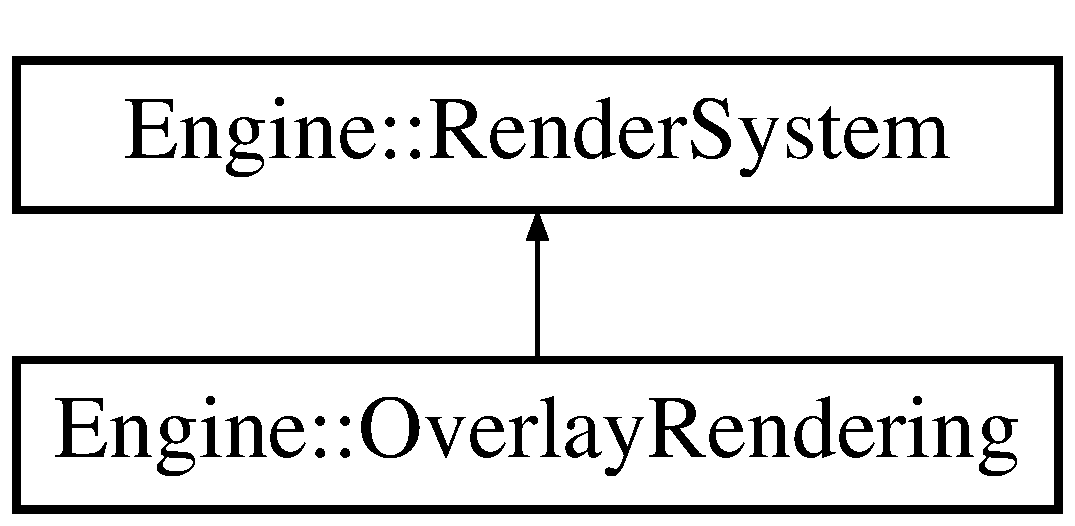
\includegraphics[height=2.000000cm]{classEngine_1_1OverlayRendering}
\end{center}
\end{figure}
\subsection*{Public Member Functions}
\begin{DoxyCompactItemize}
\item 
\hypertarget{classEngine_1_1OverlayRendering_ad6d1f4ae353491c18495a81572d20830}{}{\bfseries Overlay\+Rendering} (const std\+::string \&system\+\_\+name)\label{classEngine_1_1OverlayRendering_ad6d1f4ae353491c18495a81572d20830}

\item 
\hypertarget{classEngine_1_1OverlayRendering_afaf22f8cda0527df0b85dbce6ce5beb5}{}void {\bfseries initialize} (\hyperlink{classEngine_1_1OpenPolygonDisplay}{Open\+Polygon\+Display} $\ast$display) final override\label{classEngine_1_1OverlayRendering_afaf22f8cda0527df0b85dbce6ce5beb5}

\item 
\hypertarget{classEngine_1_1OverlayRendering_a650f19b77f1ec53974c6bbeb3b56e820}{}void {\bfseries Resize} (void) final override\label{classEngine_1_1OverlayRendering_a650f19b77f1ec53974c6bbeb3b56e820}

\item 
\hypertarget{classEngine_1_1OverlayRendering_a47c202597985d5a807c58fa4d72deba4}{}void {\bfseries Render\+Frame} (void) final override\label{classEngine_1_1OverlayRendering_a47c202597985d5a807c58fa4d72deba4}

\end{DoxyCompactItemize}
\subsection*{Protected Member Functions}
\begin{DoxyCompactItemize}
\item 
\hypertarget{classEngine_1_1OverlayRendering_a8157f82ae8e2e9d7a82759cdb4e7a8c0}{}void {\bfseries Render2\+D\+Scene} (void)\label{classEngine_1_1OverlayRendering_a8157f82ae8e2e9d7a82759cdb4e7a8c0}

\item 
\hypertarget{classEngine_1_1OverlayRendering_a5fcdc41ce4353282dad9fe2b1ca7e5e7}{}void {\bfseries Render2\+D\+Background} (void)\label{classEngine_1_1OverlayRendering_a5fcdc41ce4353282dad9fe2b1ca7e5e7}

\end{DoxyCompactItemize}
\subsection*{Additional Inherited Members}


\subsection{Detailed Description}
The \hyperlink{classEngine_1_1OverlayRendering}{Overlay\+Rendering} -\/ Render System class. 

The documentation for this class was generated from the following files\+:\begin{DoxyCompactItemize}
\item 
include/\+Render/overlayrendering.\+h\item 
Engine/\+Render/Overlay\+Rendering.\+cpp\end{DoxyCompactItemize}

\hypertarget{classEngine_1_1PanelElement}{}\section{Engine\+:\+:Panel\+Element Class Reference}
\label{classEngine_1_1PanelElement}\index{Engine\+::\+Panel\+Element@{Engine\+::\+Panel\+Element}}


The \hyperlink{classEngine_1_1PanelElement}{Panel\+Element} -\/ Panel Objective class.  




{\ttfamily \#include $<$panelelement.\+h$>$}

Inheritance diagram for Engine\+:\+:Panel\+Element\+:\begin{figure}[H]
\begin{center}
\leavevmode
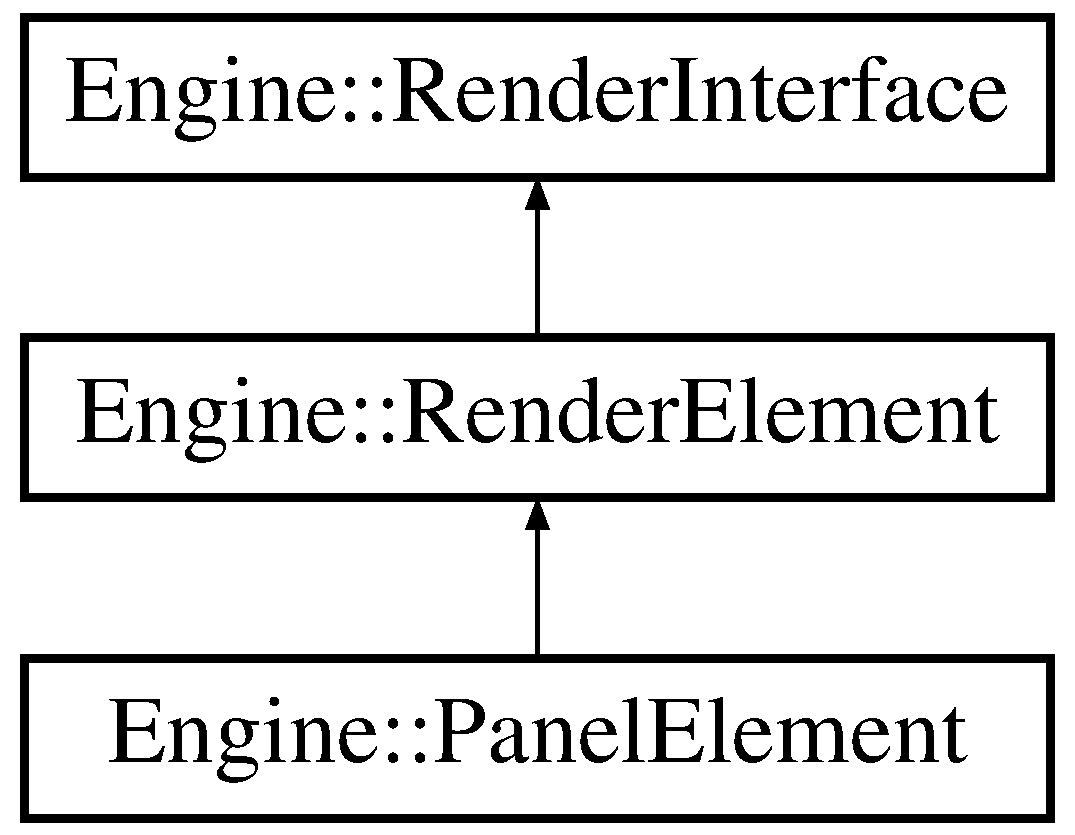
\includegraphics[height=3.000000cm]{classEngine_1_1PanelElement}
\end{center}
\end{figure}
\subsection*{Public Types}
\begin{DoxyCompactItemize}
\item 
\hypertarget{classEngine_1_1PanelElement_a2b606660873181f287c68d7b6f649821}{}enum {\bfseries Panel\+Mode} \{ {\bfseries P\+M\+\_\+\+C\+O\+L\+O\+U\+R}, 
{\bfseries P\+M\+\_\+\+T\+E\+X\+T\+U\+R\+E}
 \}\label{classEngine_1_1PanelElement_a2b606660873181f287c68d7b6f649821}

\end{DoxyCompactItemize}
\subsection*{Public Member Functions}
\begin{DoxyCompactItemize}
\item 
\hypertarget{classEngine_1_1PanelElement_a9cfb82ddfab590b5a30bb2a327b97b5a}{}{\bfseries Panel\+Element} (Panel\+Mode mode)\label{classEngine_1_1PanelElement_a9cfb82ddfab590b5a30bb2a327b97b5a}

\item 
\hypertarget{classEngine_1_1PanelElement_abf7c56c67242043a1e6a64c0a2be771b}{}void {\bfseries create} (\hyperlink{classEngine_1_1OpenPolygonDisplay}{Open\+Polygon\+Display} $\ast$display)\label{classEngine_1_1PanelElement_abf7c56c67242043a1e6a64c0a2be771b}

\item 
\hypertarget{classEngine_1_1PanelElement_a21e00e62f5776d7084ee1d3167d3e8a2}{}void {\bfseries draw} (const \hyperlink{classEngine_1_1DrawEvent}{Draw\+Event} \&event)\label{classEngine_1_1PanelElement_a21e00e62f5776d7084ee1d3167d3e8a2}

\item 
\hypertarget{classEngine_1_1PanelElement_aaaa4bacae2b01c8610125699ca9281fd}{}void {\bfseries set\+Position} (const \hyperlink{classVector3}{Vector3f} \&position)\label{classEngine_1_1PanelElement_aaaa4bacae2b01c8610125699ca9281fd}

\item 
\hypertarget{classEngine_1_1PanelElement_a6423d6f877a9238263d802c3ad815466}{}void {\bfseries set\+Scale} (const \hyperlink{classVector3}{Vector3f} \&scale)\label{classEngine_1_1PanelElement_a6423d6f877a9238263d802c3ad815466}

\item 
\hypertarget{classEngine_1_1PanelElement_acfd48ecb251bbc436cb71eb68435f0f6}{}void {\bfseries set\+Colour} (const \hyperlink{classVector4}{Vector4f} \&colour)\label{classEngine_1_1PanelElement_acfd48ecb251bbc436cb71eb68435f0f6}

\item 
\hypertarget{classEngine_1_1PanelElement_a7075c872454b272e1522a347b72d3087}{}void {\bfseries set\+Texture} (\hyperlink{classEngine_1_1Texture}{Texture} $\ast$texture)\label{classEngine_1_1PanelElement_a7075c872454b272e1522a347b72d3087}

\item 
\hypertarget{classEngine_1_1PanelElement_a1d7104eccfccf01097415933d1ff311a}{}void {\bfseries set\+Size} (const \hyperlink{classVector2}{Vector2f} \&size)\label{classEngine_1_1PanelElement_a1d7104eccfccf01097415933d1ff311a}

\item 
\hypertarget{classEngine_1_1PanelElement_a2582648d9174faac9f8d87d764b544a6}{}void {\bfseries set\+Visible} (bool status)\label{classEngine_1_1PanelElement_a2582648d9174faac9f8d87d764b544a6}

\item 
\hypertarget{classEngine_1_1PanelElement_a85a14b7b78eaddb2732869364dd819f3}{}bool {\bfseries is\+Visible} (void)\label{classEngine_1_1PanelElement_a85a14b7b78eaddb2732869364dd819f3}

\item 
\hypertarget{classEngine_1_1PanelElement_a0ebbb68be1c35ac311b0eeb9cb236849}{}\hyperlink{classVector2}{Vector2f} {\bfseries get\+Size} (void)\label{classEngine_1_1PanelElement_a0ebbb68be1c35ac311b0eeb9cb236849}

\item 
\hypertarget{classEngine_1_1PanelElement_abd71d4ff65f77f5803caea19d5d985a2}{}\hyperlink{classVector3}{Vector3f} {\bfseries get\+Absolute\+Position} (void)\label{classEngine_1_1PanelElement_abd71d4ff65f77f5803caea19d5d985a2}

\end{DoxyCompactItemize}
\subsection*{Protected Member Functions}
\begin{DoxyCompactItemize}
\item 
\hypertarget{classEngine_1_1PanelElement_a5c13bf83c13fecf8bb2d82f7571df2f1}{}void {\bfseries Draw\+Colour\+Mode} (const \hyperlink{classEngine_1_1DrawEvent}{Draw\+Event} \&event)\label{classEngine_1_1PanelElement_a5c13bf83c13fecf8bb2d82f7571df2f1}

\item 
\hypertarget{classEngine_1_1PanelElement_aa3bd2c56fe19b4ea9f4f857d02723dbd}{}void {\bfseries Draw\+Texture\+Mode} (const \hyperlink{classEngine_1_1DrawEvent}{Draw\+Event} \&event)\label{classEngine_1_1PanelElement_aa3bd2c56fe19b4ea9f4f857d02723dbd}

\end{DoxyCompactItemize}
\subsection*{Additional Inherited Members}


\subsection{Detailed Description}
The \hyperlink{classEngine_1_1PanelElement}{Panel\+Element} -\/ Panel Objective class. 

The documentation for this class was generated from the following files\+:\begin{DoxyCompactItemize}
\item 
include/panelelement.\+h\item 
Objects/\+Element/Panel\+Element.\+cpp\end{DoxyCompactItemize}

\hypertarget{classEngine_1_1PanelMouseEvent}{}\section{Engine\+:\+:Panel\+Mouse\+Event Class Reference}
\label{classEngine_1_1PanelMouseEvent}\index{Engine\+::\+Panel\+Mouse\+Event@{Engine\+::\+Panel\+Mouse\+Event}}
\subsection*{Public Member Functions}
\begin{DoxyCompactItemize}
\item 
\hypertarget{classEngine_1_1PanelMouseEvent_a7f901a923cff1561b01b958bcd93dd69}{}{\bfseries Panel\+Mouse\+Event} (\hyperlink{classEngine_1_1PanelElement}{Panel\+Element} $\ast$element, int mx, int my)\label{classEngine_1_1PanelMouseEvent_a7f901a923cff1561b01b958bcd93dd69}

\item 
\hypertarget{classEngine_1_1PanelMouseEvent_a8346dd064801f1497ca567ae06a794ae}{}\hyperlink{classEngine_1_1PanelElement}{Panel\+Element} $\ast$ {\bfseries get\+Element} (void) const \label{classEngine_1_1PanelMouseEvent_a8346dd064801f1497ca567ae06a794ae}

\item 
\hypertarget{classEngine_1_1PanelMouseEvent_a0744ce2649bf9d6fe34cfc2e538887c6}{}int {\bfseries get\+Mouse\+X} (void) const \label{classEngine_1_1PanelMouseEvent_a0744ce2649bf9d6fe34cfc2e538887c6}

\item 
\hypertarget{classEngine_1_1PanelMouseEvent_ad71770a06e7a64297f241b3c8aa11f2b}{}int {\bfseries get\+Mouse\+Y} (void) const \label{classEngine_1_1PanelMouseEvent_ad71770a06e7a64297f241b3c8aa11f2b}

\end{DoxyCompactItemize}


The documentation for this class was generated from the following file\+:\begin{DoxyCompactItemize}
\item 
include/\+Manager/userinterfacemanager.\+h\end{DoxyCompactItemize}

\hypertarget{structEngine_1_1Particle}{}\section{Engine\+:\+:Particle Struct Reference}
\label{structEngine_1_1Particle}\index{Engine\+::\+Particle@{Engine\+::\+Particle}}


The \hyperlink{structEngine_1_1Particle}{Particle} struct.  




{\ttfamily \#include $<$particleeffect.\+h$>$}

\subsection*{Public Attributes}
\begin{DoxyCompactItemize}
\item 
\hypertarget{structEngine_1_1Particle_a5bd3c23a2e7cdc8c166b75a98180e8bf}{}\hyperlink{classVector3}{Vector3f} {\bfseries position}\label{structEngine_1_1Particle_a5bd3c23a2e7cdc8c166b75a98180e8bf}

\item 
\hypertarget{structEngine_1_1Particle_a43fcf0b266f64000f8ad56265dd53be0}{}\hyperlink{classVector4}{Vector4f} {\bfseries color}\label{structEngine_1_1Particle_a43fcf0b266f64000f8ad56265dd53be0}

\item 
\hypertarget{structEngine_1_1Particle_a251e0e822d372c9a6535db59275595b4}{}int {\bfseries live}\label{structEngine_1_1Particle_a251e0e822d372c9a6535db59275595b4}

\item 
\hypertarget{structEngine_1_1Particle_a614f315262346ca051af24a1eb0a28cc}{}float {\bfseries size}\label{structEngine_1_1Particle_a614f315262346ca051af24a1eb0a28cc}

\item 
\hypertarget{structEngine_1_1Particle_af5241552092532002f63abbb5c63333d}{}float {\bfseries weight}\label{structEngine_1_1Particle_af5241552092532002f63abbb5c63333d}

\item 
\hypertarget{structEngine_1_1Particle_a7afa0ce2dde10da32acc0e70dbfb9e36}{}float {\bfseries velocity}\label{structEngine_1_1Particle_a7afa0ce2dde10da32acc0e70dbfb9e36}

\item 
\hypertarget{structEngine_1_1Particle_acbc6f4d5ffa816672fc16bdf2b2cef5e}{}float {\bfseries angle}\label{structEngine_1_1Particle_acbc6f4d5ffa816672fc16bdf2b2cef5e}

\end{DoxyCompactItemize}


\subsection{Detailed Description}
The \hyperlink{structEngine_1_1Particle}{Particle} struct. 

The documentation for this struct was generated from the following file\+:\begin{DoxyCompactItemize}
\item 
include/\+Container/particleeffect.\+h\end{DoxyCompactItemize}

\hypertarget{classEngine_1_1ParticleEffect}{}\section{Engine\+:\+:Particle\+Effect Class Reference}
\label{classEngine_1_1ParticleEffect}\index{Engine\+::\+Particle\+Effect@{Engine\+::\+Particle\+Effect}}


The \hyperlink{classEngine_1_1ParticleEffect}{Particle\+Effect} -\/ abstract class.  




{\ttfamily \#include $<$particleeffect.\+h$>$}

\subsection*{Public Member Functions}
\begin{DoxyCompactItemize}
\item 
\hypertarget{classEngine_1_1ParticleEffect_aa55c9b01da59def9254a66fe802b0e9c}{}{\bfseries Particle\+Effect} (const std\+::string \&effect\+\_\+name)\label{classEngine_1_1ParticleEffect_aa55c9b01da59def9254a66fe802b0e9c}

\item 
\hypertarget{classEngine_1_1ParticleEffect_a63cbc0e15ade08c85b5988d04b5747aa}{}virtual void {\bfseries create} (int particle\+\_\+count)\label{classEngine_1_1ParticleEffect_a63cbc0e15ade08c85b5988d04b5747aa}

\item 
\hypertarget{classEngine_1_1ParticleEffect_aaef45570f2cd8d0968730c796464723e}{}virtual void {\bfseries simulate} (float delta)=0\label{classEngine_1_1ParticleEffect_aaef45570f2cd8d0968730c796464723e}

\item 
\hypertarget{classEngine_1_1ParticleEffect_a336fe1c2e155b31790141356e310338f}{}void {\bfseries create\+Particle\+Data} (void)\label{classEngine_1_1ParticleEffect_a336fe1c2e155b31790141356e310338f}

\item 
\hypertarget{classEngine_1_1ParticleEffect_a1f599788b9ee5cfd88e05ef3de16b298}{}int {\bfseries get\+Particle\+Size} (void)\label{classEngine_1_1ParticleEffect_a1f599788b9ee5cfd88e05ef3de16b298}

\item 
\hypertarget{classEngine_1_1ParticleEffect_a8e768de548d405cdbf45fba904c87a02}{}std\+::vector$<$ float $>$ {\bfseries get\+Particle\+Vertex\+Data} ()\label{classEngine_1_1ParticleEffect_a8e768de548d405cdbf45fba904c87a02}

\item 
\hypertarget{classEngine_1_1ParticleEffect_a89ceac8e16ec44ca1862c0d07531a5ec}{}std\+::vector$<$ \hyperlink{classVector4}{Vector4f} $>$ {\bfseries get\+Particle\+T\+B\+O\+Data} ()\label{classEngine_1_1ParticleEffect_a89ceac8e16ec44ca1862c0d07531a5ec}

\end{DoxyCompactItemize}
\subsection*{Protected Attributes}
\begin{DoxyCompactItemize}
\item 
\hypertarget{classEngine_1_1ParticleEffect_a14c53c1a0dfdea8458e378772f623450}{}std\+::string {\bfseries m\+\_\+effect\+\_\+name}\label{classEngine_1_1ParticleEffect_a14c53c1a0dfdea8458e378772f623450}

\item 
\hypertarget{classEngine_1_1ParticleEffect_a34a180c3a58b998dc4ed6baf556396a4}{}std\+::vector$<$ float $>$ {\bfseries m\+\_\+particle\+\_\+vertex\+\_\+data}\label{classEngine_1_1ParticleEffect_a34a180c3a58b998dc4ed6baf556396a4}

\item 
\hypertarget{classEngine_1_1ParticleEffect_a34154c94b6eb3ee05dc4348624c2f928}{}std\+::vector$<$ \hyperlink{classVector4}{Vector4f} $>$ {\bfseries m\+\_\+particle\+\_\+tbo\+\_\+data}\label{classEngine_1_1ParticleEffect_a34154c94b6eb3ee05dc4348624c2f928}

\item 
\hypertarget{classEngine_1_1ParticleEffect_a7fe7b66f9e625e306cb7d2eb77962e4f}{}\hyperlink{classVector3}{Vector3f} {\bfseries m\+\_\+position}\label{classEngine_1_1ParticleEffect_a7fe7b66f9e625e306cb7d2eb77962e4f}

\item 
\hypertarget{classEngine_1_1ParticleEffect_a952bd22ed428ad0ac72540a2e276387c}{}Particles {\bfseries m\+\_\+particles}\label{classEngine_1_1ParticleEffect_a952bd22ed428ad0ac72540a2e276387c}

\end{DoxyCompactItemize}
\subsection*{Friends}
\begin{DoxyCompactItemize}
\item 
\hypertarget{classEngine_1_1ParticleEffect_a904cc8b18338c02f864ab20daef05c56}{}class {\bfseries Particle\+Effect\+Manager}\label{classEngine_1_1ParticleEffect_a904cc8b18338c02f864ab20daef05c56}

\item 
\hypertarget{classEngine_1_1ParticleEffect_aabcb8951071e20a007cb9a19bda2c4d3}{}class {\bfseries Particle\+Manager}\label{classEngine_1_1ParticleEffect_aabcb8951071e20a007cb9a19bda2c4d3}

\end{DoxyCompactItemize}


\subsection{Detailed Description}
The \hyperlink{classEngine_1_1ParticleEffect}{Particle\+Effect} -\/ abstract class. 

The documentation for this class was generated from the following files\+:\begin{DoxyCompactItemize}
\item 
include/\+Container/particleeffect.\+h\item 
Container/Particle\+Effect.\+cpp\end{DoxyCompactItemize}

\hypertarget{classEngine_1_1ParticleEffectManager}{}\section{Engine\+:\+:Particle\+Effect\+Manager Class Reference}
\label{classEngine_1_1ParticleEffectManager}\index{Engine\+::\+Particle\+Effect\+Manager@{Engine\+::\+Particle\+Effect\+Manager}}
Inheritance diagram for Engine\+:\+:Particle\+Effect\+Manager\+:\begin{figure}[H]
\begin{center}
\leavevmode
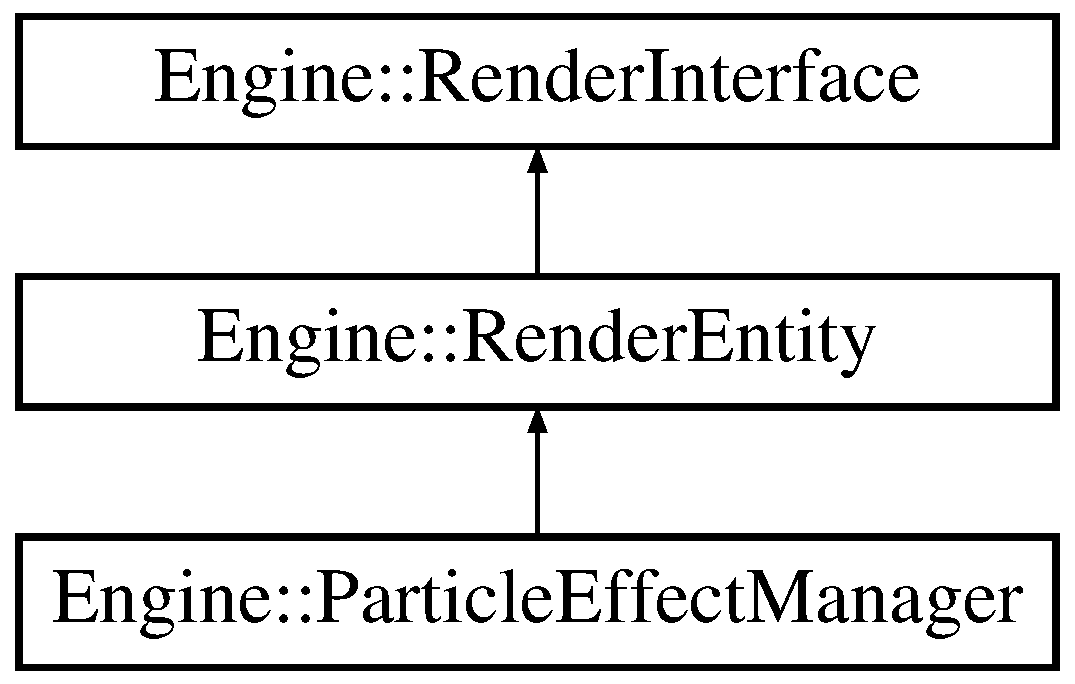
\includegraphics[height=3.000000cm]{classEngine_1_1ParticleEffectManager}
\end{center}
\end{figure}
\subsection*{Public Member Functions}
\begin{DoxyCompactItemize}
\item 
\hypertarget{classEngine_1_1ParticleEffectManager_a86f690f39fcef9dabfec281bffb80e14}{}{\bfseries Particle\+Effect\+Manager} (\hyperlink{classEngine_1_1OpenPolygonDisplay}{Open\+Polygon\+Display} $\ast$display)\label{classEngine_1_1ParticleEffectManager_a86f690f39fcef9dabfec281bffb80e14}

\item 
\hypertarget{classEngine_1_1ParticleEffectManager_ae016d027787d8fac9db8dd59ccc94e27}{}void {\bfseries create} (\hyperlink{classEngine_1_1OpenPolygonDisplay}{Open\+Polygon\+Display} $\ast$display)\label{classEngine_1_1ParticleEffectManager_ae016d027787d8fac9db8dd59ccc94e27}

\item 
\hypertarget{classEngine_1_1ParticleEffectManager_a2afa33d7418ddb473429bd17fbfc6938}{}void {\bfseries draw} (const \hyperlink{classEngine_1_1DrawEvent}{Draw\+Event} \&event)\label{classEngine_1_1ParticleEffectManager_a2afa33d7418ddb473429bd17fbfc6938}

\item 
\hypertarget{classEngine_1_1ParticleEffectManager_a6c801aa851b3b8356af24664f7fef447}{}void {\bfseries initialize} (void)\label{classEngine_1_1ParticleEffectManager_a6c801aa851b3b8356af24664f7fef447}

\item 
\hypertarget{classEngine_1_1ParticleEffectManager_ad877db180062f34aac1460eebcd7ca78}{}void {\bfseries initialize} (const std\+::string \&mesh\+\_\+name)\label{classEngine_1_1ParticleEffectManager_ad877db180062f34aac1460eebcd7ca78}

\item 
\hypertarget{classEngine_1_1ParticleEffectManager_ada3f0a45f95007e41ce2cced7eba1eab}{}void {\bfseries initialize} (\hyperlink{classEngine_1_1Mesh}{Mesh} $\ast$mesh)\label{classEngine_1_1ParticleEffectManager_ada3f0a45f95007e41ce2cced7eba1eab}

\item 
\hypertarget{classEngine_1_1ParticleEffectManager_a3779524ad57f1c962b91c6f195b7b5cf}{}void {\bfseries add\+Effect} (\hyperlink{classEngine_1_1ParticleEffect}{Particle\+Effect} $\ast$effect, int particle\+\_\+count)\label{classEngine_1_1ParticleEffectManager_a3779524ad57f1c962b91c6f195b7b5cf}

\item 
\hypertarget{classEngine_1_1ParticleEffectManager_aa702c07d7043427cd78e9518ff0512d2}{}void {\bfseries render} (const std\+::string \&effect\+\_\+name, const \hyperlink{classEngine_1_1DrawEvent}{Draw\+Event} \&event)\label{classEngine_1_1ParticleEffectManager_aa702c07d7043427cd78e9518ff0512d2}

\item 
\hypertarget{classEngine_1_1ParticleEffectManager_ac52f3d3ce284d80422388d7149171d96}{}void {\bfseries render} (\hyperlink{classEngine_1_1ParticleEffect}{Particle\+Effect} $\ast$effect, const \hyperlink{classEngine_1_1DrawEvent}{Draw\+Event} \&event)\label{classEngine_1_1ParticleEffectManager_ac52f3d3ce284d80422388d7149171d96}

\item 
\hypertarget{classEngine_1_1ParticleEffectManager_a337f876c0f75f7f3dc8e4896f97eba79}{}bool {\bfseries is\+Initialized} (void)\label{classEngine_1_1ParticleEffectManager_a337f876c0f75f7f3dc8e4896f97eba79}

\item 
\hypertarget{classEngine_1_1ParticleEffectManager_a9b05d928b05118f50ab13f69c1a182bf}{}\hyperlink{classEngine_1_1ParticleEffect}{Particle\+Effect} $\ast$ {\bfseries get\+Effect} (const std\+::string \&effect\+\_\+name)\label{classEngine_1_1ParticleEffectManager_a9b05d928b05118f50ab13f69c1a182bf}

\item 
\hypertarget{classEngine_1_1ParticleEffectManager_af652b0b637a88347b521d4b792f857fe}{}void {\bfseries remove} (\hyperlink{classEngine_1_1ParticleEffect}{Particle\+Effect} $\ast$effect)\label{classEngine_1_1ParticleEffectManager_af652b0b637a88347b521d4b792f857fe}

\item 
\hypertarget{classEngine_1_1ParticleEffectManager_a7f8e7adfa89a979a9927c7bcd48ffc85}{}void {\bfseries remove} (const std\+::string \&effect\+\_\+name)\label{classEngine_1_1ParticleEffectManager_a7f8e7adfa89a979a9927c7bcd48ffc85}

\item 
\hypertarget{classEngine_1_1ParticleEffectManager_a019213e48edc21b007129b900c77cd65}{}Particle\+Effects {\bfseries get\+Effects} (void)\label{classEngine_1_1ParticleEffectManager_a019213e48edc21b007129b900c77cd65}

\end{DoxyCompactItemize}
\subsection*{Additional Inherited Members}


The documentation for this class was generated from the following files\+:\begin{DoxyCompactItemize}
\item 
include/\+Manager/particleeffectmanager.\+h\item 
Engine/\+Manager/Particle\+Effect\+Manager.\+cpp\end{DoxyCompactItemize}

\hypertarget{classEngine_1_1ParticleManager}{}\section{Engine\+:\+:Particle\+Manager Class Reference}
\label{classEngine_1_1ParticleManager}\index{Engine\+::\+Particle\+Manager@{Engine\+::\+Particle\+Manager}}
\subsection*{Public Member Functions}
\begin{DoxyCompactItemize}
\item 
\hypertarget{classEngine_1_1ParticleManager_af4e8e3bdfea5a45e1f2c9bf6ec7dce0e}{}void {\bfseries add\+Effect} (\hyperlink{classEngine_1_1ParticleEffect}{Particle\+Effect} $\ast$effect, int particle\+\_\+count)\label{classEngine_1_1ParticleManager_af4e8e3bdfea5a45e1f2c9bf6ec7dce0e}

\item 
\hypertarget{classEngine_1_1ParticleManager_a59de97280e9f50e36a84f440a8ee7258}{}void {\bfseries remove} (\hyperlink{classEngine_1_1ParticleEffect}{Particle\+Effect} $\ast$effect)\label{classEngine_1_1ParticleManager_a59de97280e9f50e36a84f440a8ee7258}

\item 
\hypertarget{classEngine_1_1ParticleManager_a46eec3d233c700e30f0aa634ae52ee05}{}void {\bfseries remove} (const std\+::string \&effect\+\_\+name)\label{classEngine_1_1ParticleManager_a46eec3d233c700e30f0aa634ae52ee05}

\item 
\hypertarget{classEngine_1_1ParticleManager_a1a013ffb83f07305275b14c7adf20266}{}void {\bfseries remove\+All} (void)\label{classEngine_1_1ParticleManager_a1a013ffb83f07305275b14c7adf20266}

\item 
\hypertarget{classEngine_1_1ParticleManager_aa1bbafc5b5aef986d9f74d7fb6a0319c}{}void {\bfseries trigger} (\hyperlink{classEngine_1_1ParticleEffect}{Particle\+Effect} $\ast$effect)\label{classEngine_1_1ParticleManager_aa1bbafc5b5aef986d9f74d7fb6a0319c}

\item 
\hypertarget{classEngine_1_1ParticleManager_ad6e84805149854b1622b0f71b5664c52}{}void {\bfseries trigger} (const std\+::string \&effect\+\_\+name)\label{classEngine_1_1ParticleManager_ad6e84805149854b1622b0f71b5664c52}

\item 
\hypertarget{classEngine_1_1ParticleManager_a3ab9fc206bec8e349e810fecf53ab7f2}{}Particle\+Effects {\bfseries get\+Particle\+Effects} (void)\label{classEngine_1_1ParticleManager_a3ab9fc206bec8e349e810fecf53ab7f2}

\item 
\hypertarget{classEngine_1_1ParticleManager_aaa00547e7bd702f2707e1828eb2d77d6}{}\hyperlink{classEngine_1_1ParticleEffect}{Particle\+Effect} $\ast$ {\bfseries get\+Effect} (const std\+::string \&effect\+\_\+name)\label{classEngine_1_1ParticleManager_aaa00547e7bd702f2707e1828eb2d77d6}

\end{DoxyCompactItemize}
\subsection*{Static Public Member Functions}
\begin{DoxyCompactItemize}
\item 
\hypertarget{classEngine_1_1ParticleManager_aef6ab3d8b2184bc87ae179625b532546}{}static \hyperlink{classEngine_1_1ParticleManager}{Particle\+Manager} $\ast$ {\bfseries get\+Singleton\+Ptr} (void)\label{classEngine_1_1ParticleManager_aef6ab3d8b2184bc87ae179625b532546}

\end{DoxyCompactItemize}


The documentation for this class was generated from the following files\+:\begin{DoxyCompactItemize}
\item 
include/\+Manager/particlemanager.\+h\item 
Engine/\+Manager/Particle\+Manager.\+cpp\end{DoxyCompactItemize}

\hypertarget{structEngine_1_1PixelCoordData}{}\section{Engine\+:\+:Pixel\+Coord\+Data Struct Reference}
\label{structEngine_1_1PixelCoordData}\index{Engine\+::\+Pixel\+Coord\+Data@{Engine\+::\+Pixel\+Coord\+Data}}
\subsection*{Public Attributes}
\begin{DoxyCompactItemize}
\item 
\hypertarget{structEngine_1_1PixelCoordData_a9cbdb8651e5e3e35f6ca1d18d90fc03e}{}\hyperlink{classVector2}{Vector2i} {\bfseries terrain\+\_\+size}\label{structEngine_1_1PixelCoordData_a9cbdb8651e5e3e35f6ca1d18d90fc03e}

\item 
\hypertarget{structEngine_1_1PixelCoordData_a72bdec3875808ed3e086272c687a3a4a}{}\hyperlink{classVector2}{Vector2i} {\bfseries texture\+\_\+size}\label{structEngine_1_1PixelCoordData_a72bdec3875808ed3e086272c687a3a4a}

\item 
\hypertarget{structEngine_1_1PixelCoordData_abc0179853658fda0f0f0e65d2f856c33}{}\hyperlink{classVector2}{Vector2f} {\bfseries player\+\_\+pos}\label{structEngine_1_1PixelCoordData_abc0179853658fda0f0f0e65d2f856c33}

\end{DoxyCompactItemize}


The documentation for this struct was generated from the following file\+:\begin{DoxyCompactItemize}
\item 
include/eutils.\+h\end{DoxyCompactItemize}

\hypertarget{classEngine_1_1Position}{}\section{Engine\+:\+:Position Class Reference}
\label{classEngine_1_1Position}\index{Engine\+::\+Position@{Engine\+::\+Position}}


The \hyperlink{classEngine_1_1Position}{Position} class.  




{\ttfamily \#include $<$position.\+h$>$}

Inheritance diagram for Engine\+:\+:Position\+:\begin{figure}[H]
\begin{center}
\leavevmode
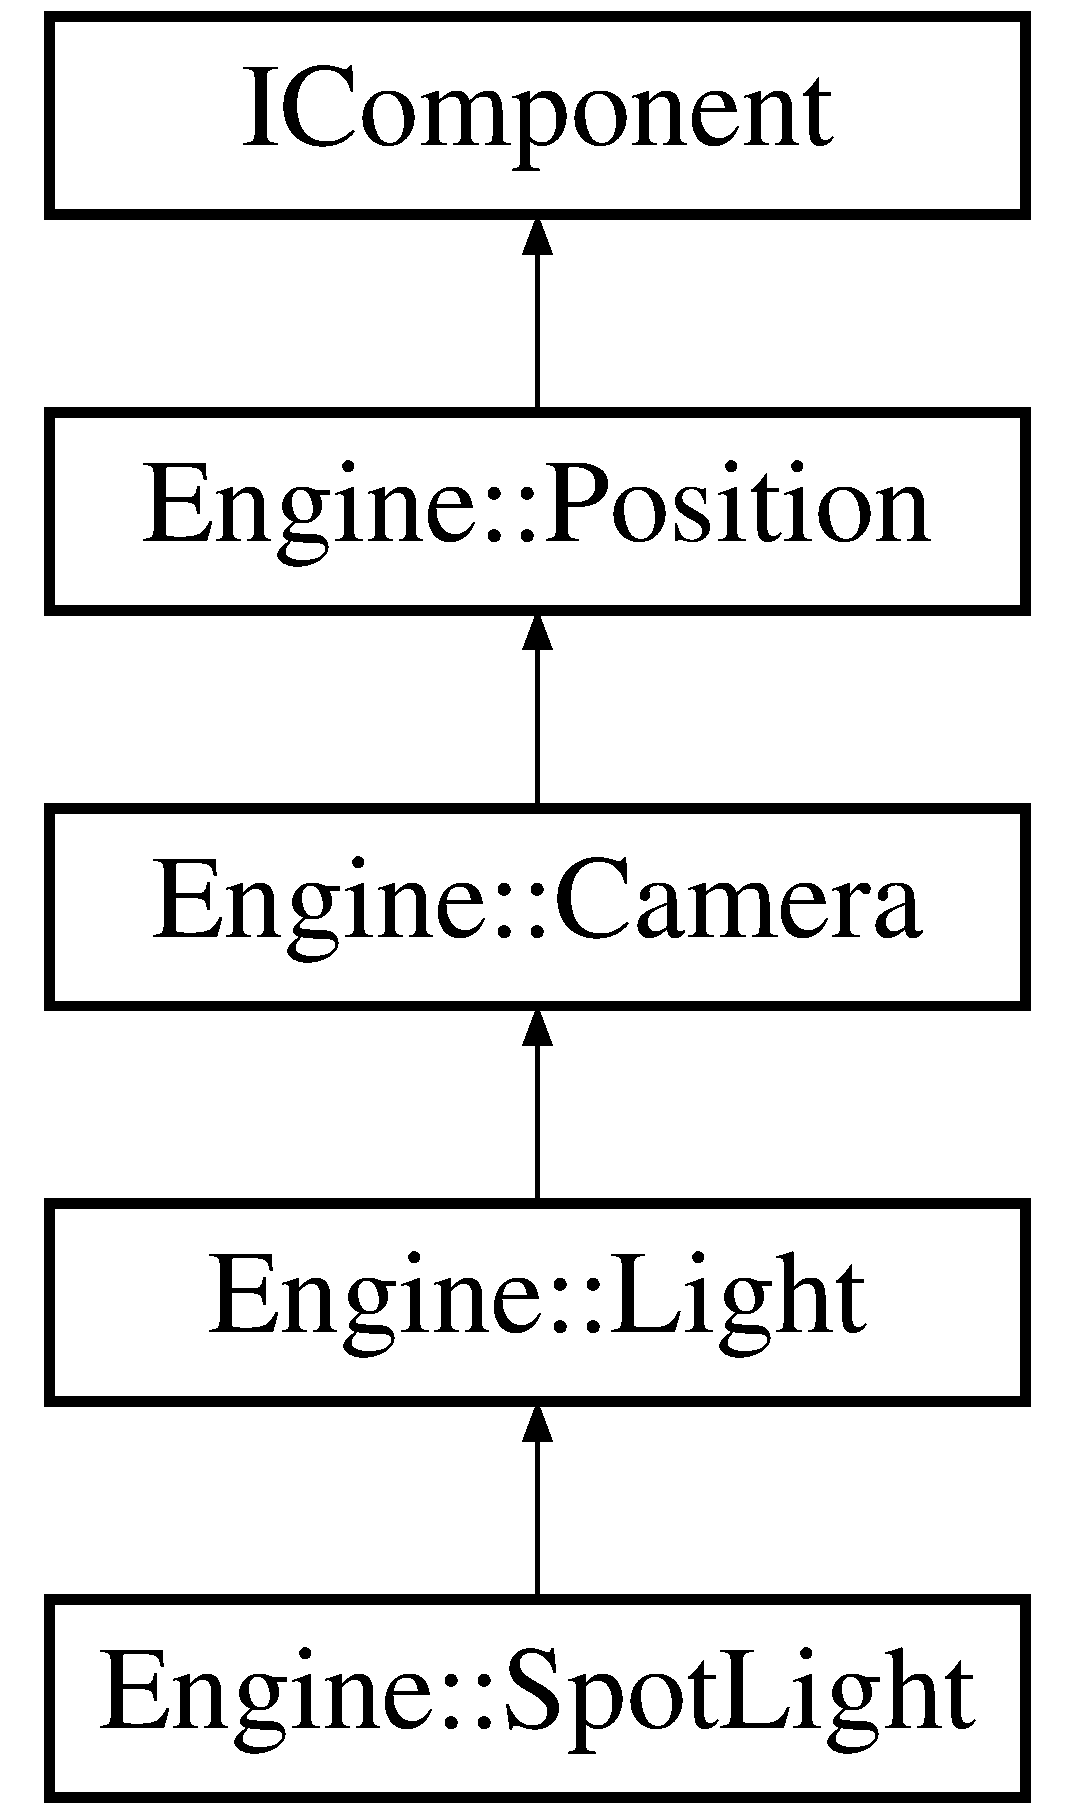
\includegraphics[height=5.000000cm]{classEngine_1_1Position}
\end{center}
\end{figure}
\subsection*{Public Member Functions}
\begin{DoxyCompactItemize}
\item 
\hypertarget{classEngine_1_1Position_a0272e50c356513dd03d8bcae988bc6c1}{}{\bfseries Position} (const std\+::string \&component\+\_\+name)\label{classEngine_1_1Position_a0272e50c356513dd03d8bcae988bc6c1}

\item 
void \hyperlink{classEngine_1_1Position_af4faa47a68f4fb9c2e98313e3f4244d8}{set\+Position} (const \hyperlink{classVector3}{Vector3f} \&position)
\begin{DoxyCompactList}\small\item\em set\+Position \end{DoxyCompactList}\item 
void \hyperlink{classEngine_1_1Position_a145a53d6a9842f2c9ce9e238eb21884f}{set\+Rotation} (const \hyperlink{classVector3}{Vector3f} \&rotation)
\begin{DoxyCompactList}\small\item\em set\+Rotation \end{DoxyCompactList}\item 
void \hyperlink{classEngine_1_1Position_a2e42fbf00ddfac1b1c1b92baa9e03b87}{set\+Scale} (const \hyperlink{classVector3}{Vector3f} \&scale)
\begin{DoxyCompactList}\small\item\em set\+Scale \end{DoxyCompactList}\item 
void \hyperlink{classEngine_1_1Position_a396150281cfa2604a48b7f90fc858b9c}{set\+Quanternion} (const \hyperlink{classVector4}{Vector4f} \&quant)
\begin{DoxyCompactList}\small\item\em set\+Quanternion \end{DoxyCompactList}\item 
void \hyperlink{classEngine_1_1Position_a1daaa95f7197ef1f2ecbcc29639d3040}{set\+Matrix} (const glm\+::mat4 \&model\+\_\+matrix)
\begin{DoxyCompactList}\small\item\em set\+Matrix \end{DoxyCompactList}\item 
const \hyperlink{classVector3}{Vector3f} \& \hyperlink{classEngine_1_1Position_a91f993c0f10be51167737aad36065188}{get\+Position} (void) const 
\begin{DoxyCompactList}\small\item\em get\+Position \end{DoxyCompactList}\item 
const \hyperlink{classVector3}{Vector3f} \& \hyperlink{classEngine_1_1Position_aa13ac4ee93439ff53585b719be6b4066}{get\+Rotation} (void) const 
\begin{DoxyCompactList}\small\item\em get\+Rotation \end{DoxyCompactList}\item 
const \hyperlink{classVector3}{Vector3f} \& \hyperlink{classEngine_1_1Position_a11cd4d028d14646d067437cfd087b057}{get\+Scale} (void) const 
\begin{DoxyCompactList}\small\item\em get\+Scale \end{DoxyCompactList}\item 
const \hyperlink{classVector4}{Vector4f} \& \hyperlink{classEngine_1_1Position_a2d7b2153822522b82221b7fb470fad73}{get\+Quanternion} (void) const 
\begin{DoxyCompactList}\small\item\em get\+Quanternion \end{DoxyCompactList}\item 
glm\+::quat \hyperlink{classEngine_1_1Position_a4dabca5c3401e511e79bb305fecabb5e}{get\+Quat} () const 
\begin{DoxyCompactList}\small\item\em get\+Quat \end{DoxyCompactList}\item 
\hypertarget{classEngine_1_1Position_a4fa18114d2f27699c90822e61a7fbbab}{}glm\+::mat4 {\bfseries get\+Translation\+Matrix} (glm\+::vec3 vector)\label{classEngine_1_1Position_a4fa18114d2f27699c90822e61a7fbbab}

\item 
glm\+::mat4 \hyperlink{classEngine_1_1Position_a1da72afb76b823fbe3036603c5c13daf}{get\+Translation\+Matrix} (void) const 
\begin{DoxyCompactList}\small\item\em get\+Translation\+Matrix \end{DoxyCompactList}\item 
glm\+::mat4 \hyperlink{classEngine_1_1Position_a9aaab620b558cfaa13549368fdfd25cf}{get\+Rotation\+Matrix} (void) const 
\begin{DoxyCompactList}\small\item\em get\+Rotation\+Matrix \end{DoxyCompactList}\item 
\hypertarget{classEngine_1_1Position_a2a1f69f40dd519292df5f2bb0be86a0a}{}glm\+::mat4 {\bfseries get\+Rotation\+Matrix} (const \hyperlink{classVector3}{Vector3f} \&vector)\label{classEngine_1_1Position_a2a1f69f40dd519292df5f2bb0be86a0a}

\item 
glm\+::mat4 \hyperlink{classEngine_1_1Position_a1078fe747a66ee2f189f6e0039cf6471}{get\+Matrix} (void) const 
\begin{DoxyCompactList}\small\item\em get\+Matrix \end{DoxyCompactList}\item 
glm\+::mat4 \hyperlink{classEngine_1_1Position_add58d052693b4009a03fef44bed96fe2}{get\+Normal\+Matrix} (glm\+::mat4 model\+\_\+view) const 
\begin{DoxyCompactList}\small\item\em get\+Normal\+Matrix \end{DoxyCompactList}\item 
void \hyperlink{classEngine_1_1Position_ac8789d4c6275c4525c2933c7a5344a05}{camtransformation} (void)
\begin{DoxyCompactList}\small\item\em camtransformation \end{DoxyCompactList}\item 
void \hyperlink{classEngine_1_1Position_ac257e9c6271c3b3345f9a33cb6c33356}{transformation} (void)
\begin{DoxyCompactList}\small\item\em transformation \end{DoxyCompactList}\end{DoxyCompactItemize}


\subsection{Detailed Description}
The \hyperlink{classEngine_1_1Position}{Position} class. 

Save Model\+Matrix Data 

\subsection{Member Function Documentation}
\hypertarget{classEngine_1_1Position_ac8789d4c6275c4525c2933c7a5344a05}{}\index{Engine\+::\+Position@{Engine\+::\+Position}!camtransformation@{camtransformation}}
\index{camtransformation@{camtransformation}!Engine\+::\+Position@{Engine\+::\+Position}}
\subsubsection[{camtransformation(void)}]{\setlength{\rightskip}{0pt plus 5cm}void Position\+::camtransformation (
\begin{DoxyParamCaption}
\item[{void}]{}
\end{DoxyParamCaption}
)}\label{classEngine_1_1Position_ac8789d4c6275c4525c2933c7a5344a05}


camtransformation 

\hyperlink{classEngine_1_1Camera}{Camera} Transformation -\/ Load Model\+Matrix \hypertarget{classEngine_1_1Position_a1078fe747a66ee2f189f6e0039cf6471}{}\index{Engine\+::\+Position@{Engine\+::\+Position}!get\+Matrix@{get\+Matrix}}
\index{get\+Matrix@{get\+Matrix}!Engine\+::\+Position@{Engine\+::\+Position}}
\subsubsection[{get\+Matrix(void) const }]{\setlength{\rightskip}{0pt plus 5cm}glm\+::mat4 Position\+::get\+Matrix (
\begin{DoxyParamCaption}
\item[{void}]{}
\end{DoxyParamCaption}
) const}\label{classEngine_1_1Position_a1078fe747a66ee2f189f6e0039cf6471}


get\+Matrix 

Return Model Matrix \begin{DoxyReturn}{Returns}

\end{DoxyReturn}
\hypertarget{classEngine_1_1Position_add58d052693b4009a03fef44bed96fe2}{}\index{Engine\+::\+Position@{Engine\+::\+Position}!get\+Normal\+Matrix@{get\+Normal\+Matrix}}
\index{get\+Normal\+Matrix@{get\+Normal\+Matrix}!Engine\+::\+Position@{Engine\+::\+Position}}
\subsubsection[{get\+Normal\+Matrix(glm\+::mat4 model\+\_\+view) const }]{\setlength{\rightskip}{0pt plus 5cm}glm\+::mat4 Position\+::get\+Normal\+Matrix (
\begin{DoxyParamCaption}
\item[{glm\+::mat4}]{model\+\_\+view}
\end{DoxyParamCaption}
) const}\label{classEngine_1_1Position_add58d052693b4009a03fef44bed96fe2}


get\+Normal\+Matrix 

Return Normal Matrix 
\begin{DoxyParams}{Parameters}
{\em model\+\_\+view} & \\
\hline
\end{DoxyParams}
\begin{DoxyReturn}{Returns}

\end{DoxyReturn}
\hypertarget{classEngine_1_1Position_a91f993c0f10be51167737aad36065188}{}\index{Engine\+::\+Position@{Engine\+::\+Position}!get\+Position@{get\+Position}}
\index{get\+Position@{get\+Position}!Engine\+::\+Position@{Engine\+::\+Position}}
\subsubsection[{get\+Position(void) const }]{\setlength{\rightskip}{0pt plus 5cm}const {\bf Vector3f} \& Position\+::get\+Position (
\begin{DoxyParamCaption}
\item[{void}]{}
\end{DoxyParamCaption}
) const}\label{classEngine_1_1Position_a91f993c0f10be51167737aad36065188}


get\+Position 

Return Positions \begin{DoxyReturn}{Returns}

\end{DoxyReturn}
\hypertarget{classEngine_1_1Position_a2d7b2153822522b82221b7fb470fad73}{}\index{Engine\+::\+Position@{Engine\+::\+Position}!get\+Quanternion@{get\+Quanternion}}
\index{get\+Quanternion@{get\+Quanternion}!Engine\+::\+Position@{Engine\+::\+Position}}
\subsubsection[{get\+Quanternion(void) const }]{\setlength{\rightskip}{0pt plus 5cm}const {\bf Vector4f} \& Position\+::get\+Quanternion (
\begin{DoxyParamCaption}
\item[{void}]{}
\end{DoxyParamCaption}
) const}\label{classEngine_1_1Position_a2d7b2153822522b82221b7fb470fad73}


get\+Quanternion 

Return Quaternion \begin{DoxyReturn}{Returns}

\end{DoxyReturn}
\hypertarget{classEngine_1_1Position_a4dabca5c3401e511e79bb305fecabb5e}{}\index{Engine\+::\+Position@{Engine\+::\+Position}!get\+Quat@{get\+Quat}}
\index{get\+Quat@{get\+Quat}!Engine\+::\+Position@{Engine\+::\+Position}}
\subsubsection[{get\+Quat() const }]{\setlength{\rightskip}{0pt plus 5cm}glm\+::quat Position\+::get\+Quat (
\begin{DoxyParamCaption}
\item[{void}]{}
\end{DoxyParamCaption}
) const}\label{classEngine_1_1Position_a4dabca5c3401e511e79bb305fecabb5e}


get\+Quat 

Return Quaternion \begin{DoxyReturn}{Returns}

\end{DoxyReturn}
\hypertarget{classEngine_1_1Position_aa13ac4ee93439ff53585b719be6b4066}{}\index{Engine\+::\+Position@{Engine\+::\+Position}!get\+Rotation@{get\+Rotation}}
\index{get\+Rotation@{get\+Rotation}!Engine\+::\+Position@{Engine\+::\+Position}}
\subsubsection[{get\+Rotation(void) const }]{\setlength{\rightskip}{0pt plus 5cm}const {\bf Vector3f} \& Position\+::get\+Rotation (
\begin{DoxyParamCaption}
\item[{void}]{}
\end{DoxyParamCaption}
) const}\label{classEngine_1_1Position_aa13ac4ee93439ff53585b719be6b4066}


get\+Rotation 

Return Rotation \begin{DoxyReturn}{Returns}

\end{DoxyReturn}
\hypertarget{classEngine_1_1Position_a9aaab620b558cfaa13549368fdfd25cf}{}\index{Engine\+::\+Position@{Engine\+::\+Position}!get\+Rotation\+Matrix@{get\+Rotation\+Matrix}}
\index{get\+Rotation\+Matrix@{get\+Rotation\+Matrix}!Engine\+::\+Position@{Engine\+::\+Position}}
\subsubsection[{get\+Rotation\+Matrix(void) const }]{\setlength{\rightskip}{0pt plus 5cm}glm\+::mat4 Position\+::get\+Rotation\+Matrix (
\begin{DoxyParamCaption}
\item[{void}]{}
\end{DoxyParamCaption}
) const}\label{classEngine_1_1Position_a9aaab620b558cfaa13549368fdfd25cf}


get\+Rotation\+Matrix 

Return only Rotation Matrix \begin{DoxyReturn}{Returns}

\end{DoxyReturn}
\hypertarget{classEngine_1_1Position_a11cd4d028d14646d067437cfd087b057}{}\index{Engine\+::\+Position@{Engine\+::\+Position}!get\+Scale@{get\+Scale}}
\index{get\+Scale@{get\+Scale}!Engine\+::\+Position@{Engine\+::\+Position}}
\subsubsection[{get\+Scale(void) const }]{\setlength{\rightskip}{0pt plus 5cm}const {\bf Vector3f} \& Position\+::get\+Scale (
\begin{DoxyParamCaption}
\item[{void}]{}
\end{DoxyParamCaption}
) const}\label{classEngine_1_1Position_a11cd4d028d14646d067437cfd087b057}


get\+Scale 

Return Scale \begin{DoxyReturn}{Returns}

\end{DoxyReturn}
\hypertarget{classEngine_1_1Position_a1da72afb76b823fbe3036603c5c13daf}{}\index{Engine\+::\+Position@{Engine\+::\+Position}!get\+Translation\+Matrix@{get\+Translation\+Matrix}}
\index{get\+Translation\+Matrix@{get\+Translation\+Matrix}!Engine\+::\+Position@{Engine\+::\+Position}}
\subsubsection[{get\+Translation\+Matrix(void) const }]{\setlength{\rightskip}{0pt plus 5cm}glm\+::mat4 Position\+::get\+Translation\+Matrix (
\begin{DoxyParamCaption}
\item[{void}]{}
\end{DoxyParamCaption}
) const}\label{classEngine_1_1Position_a1da72afb76b823fbe3036603c5c13daf}


get\+Translation\+Matrix 

\begin{DoxyReturn}{Returns}

\end{DoxyReturn}
\hypertarget{classEngine_1_1Position_a1daaa95f7197ef1f2ecbcc29639d3040}{}\index{Engine\+::\+Position@{Engine\+::\+Position}!set\+Matrix@{set\+Matrix}}
\index{set\+Matrix@{set\+Matrix}!Engine\+::\+Position@{Engine\+::\+Position}}
\subsubsection[{set\+Matrix(const glm\+::mat4 \&model\+\_\+matrix)}]{\setlength{\rightskip}{0pt plus 5cm}void Position\+::set\+Matrix (
\begin{DoxyParamCaption}
\item[{const glm\+::mat4 \&}]{model\+\_\+matrix}
\end{DoxyParamCaption}
)}\label{classEngine_1_1Position_a1daaa95f7197ef1f2ecbcc29639d3040}


set\+Matrix 

Set Model Matrix 
\begin{DoxyParams}{Parameters}
{\em model\+\_\+matrix} & \\
\hline
\end{DoxyParams}
\hypertarget{classEngine_1_1Position_af4faa47a68f4fb9c2e98313e3f4244d8}{}\index{Engine\+::\+Position@{Engine\+::\+Position}!set\+Position@{set\+Position}}
\index{set\+Position@{set\+Position}!Engine\+::\+Position@{Engine\+::\+Position}}
\subsubsection[{set\+Position(const Vector3f \&position)}]{\setlength{\rightskip}{0pt plus 5cm}void Position\+::set\+Position (
\begin{DoxyParamCaption}
\item[{const {\bf Vector3f} \&}]{position}
\end{DoxyParamCaption}
)}\label{classEngine_1_1Position_af4faa47a68f4fb9c2e98313e3f4244d8}


set\+Position 

Set \hyperlink{classEngine_1_1Position}{Position} 
\begin{DoxyParams}{Parameters}
{\em position} & \\
\hline
\end{DoxyParams}
\hypertarget{classEngine_1_1Position_a396150281cfa2604a48b7f90fc858b9c}{}\index{Engine\+::\+Position@{Engine\+::\+Position}!set\+Quanternion@{set\+Quanternion}}
\index{set\+Quanternion@{set\+Quanternion}!Engine\+::\+Position@{Engine\+::\+Position}}
\subsubsection[{set\+Quanternion(const Vector4f \&quant)}]{\setlength{\rightskip}{0pt plus 5cm}void Position\+::set\+Quanternion (
\begin{DoxyParamCaption}
\item[{const {\bf Vector4f} \&}]{quant}
\end{DoxyParamCaption}
)}\label{classEngine_1_1Position_a396150281cfa2604a48b7f90fc858b9c}


set\+Quanternion 

Set Quaternion 
\begin{DoxyParams}{Parameters}
{\em quant} & \\
\hline
\end{DoxyParams}
\hypertarget{classEngine_1_1Position_a145a53d6a9842f2c9ce9e238eb21884f}{}\index{Engine\+::\+Position@{Engine\+::\+Position}!set\+Rotation@{set\+Rotation}}
\index{set\+Rotation@{set\+Rotation}!Engine\+::\+Position@{Engine\+::\+Position}}
\subsubsection[{set\+Rotation(const Vector3f \&rotation)}]{\setlength{\rightskip}{0pt plus 5cm}void Position\+::set\+Rotation (
\begin{DoxyParamCaption}
\item[{const {\bf Vector3f} \&}]{rotation}
\end{DoxyParamCaption}
)}\label{classEngine_1_1Position_a145a53d6a9842f2c9ce9e238eb21884f}


set\+Rotation 

Set Rotation 
\begin{DoxyParams}{Parameters}
{\em rotation} & \\
\hline
\end{DoxyParams}
\hypertarget{classEngine_1_1Position_a2e42fbf00ddfac1b1c1b92baa9e03b87}{}\index{Engine\+::\+Position@{Engine\+::\+Position}!set\+Scale@{set\+Scale}}
\index{set\+Scale@{set\+Scale}!Engine\+::\+Position@{Engine\+::\+Position}}
\subsubsection[{set\+Scale(const Vector3f \&scale)}]{\setlength{\rightskip}{0pt plus 5cm}void Position\+::set\+Scale (
\begin{DoxyParamCaption}
\item[{const {\bf Vector3f} \&}]{scale}
\end{DoxyParamCaption}
)}\label{classEngine_1_1Position_a2e42fbf00ddfac1b1c1b92baa9e03b87}


set\+Scale 

Set Scale 
\begin{DoxyParams}{Parameters}
{\em scale} & \\
\hline
\end{DoxyParams}
\hypertarget{classEngine_1_1Position_ac257e9c6271c3b3345f9a33cb6c33356}{}\index{Engine\+::\+Position@{Engine\+::\+Position}!transformation@{transformation}}
\index{transformation@{transformation}!Engine\+::\+Position@{Engine\+::\+Position}}
\subsubsection[{transformation(void)}]{\setlength{\rightskip}{0pt plus 5cm}void Position\+::transformation (
\begin{DoxyParamCaption}
\item[{void}]{}
\end{DoxyParamCaption}
)}\label{classEngine_1_1Position_ac257e9c6271c3b3345f9a33cb6c33356}


transformation 

Normal Object Transformation -\/ Load Model\+Matrix 

The documentation for this class was generated from the following files\+:\begin{DoxyCompactItemize}
\item 
include/\+Container/position.\+h\item 
Container/Position.\+cpp\end{DoxyCompactItemize}

\hypertarget{classEngine_1_1PositionManager}{}\section{Engine\+:\+:Position\+Manager Class Reference}
\label{classEngine_1_1PositionManager}\index{Engine\+::\+Position\+Manager@{Engine\+::\+Position\+Manager}}


The \hyperlink{classEngine_1_1PositionManager}{Position\+Manager} class.  




{\ttfamily \#include $<$positionmanager.\+h$>$}

Inheritance diagram for Engine\+:\+:Position\+Manager\+:\begin{figure}[H]
\begin{center}
\leavevmode
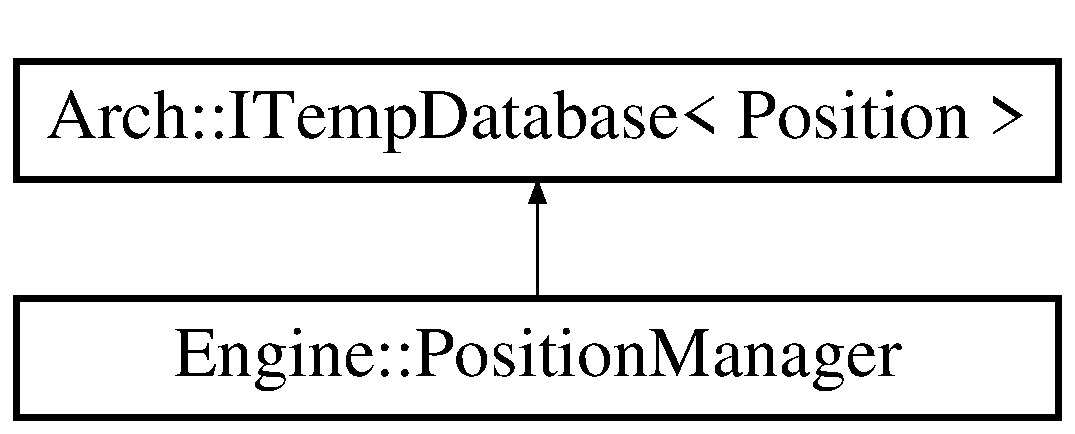
\includegraphics[height=2.000000cm]{classEngine_1_1PositionManager}
\end{center}
\end{figure}
\subsection*{Public Member Functions}
\begin{DoxyCompactItemize}
\item 
\hypertarget{classEngine_1_1PositionManager_a3ffde9f48538c6a16d9ec84e8c73dd21}{}\hyperlink{classEngine_1_1Position}{Position} $\ast$ {\bfseries create\+Position} (void)\label{classEngine_1_1PositionManager_a3ffde9f48538c6a16d9ec84e8c73dd21}

\item 
\hypertarget{classEngine_1_1PositionManager_ab25d55ad5c140fa7f71e2303b74fe6da}{}\hyperlink{classEngine_1_1Position}{Position} $\ast$ {\bfseries get\+Position} (uint container\+\_\+id)\label{classEngine_1_1PositionManager_ab25d55ad5c140fa7f71e2303b74fe6da}

\item 
\hypertarget{classEngine_1_1PositionManager_a77166e3a79017c8f2cb179828812bc31}{}void {\bfseries destroy} (uint container\+\_\+id)\label{classEngine_1_1PositionManager_a77166e3a79017c8f2cb179828812bc31}

\end{DoxyCompactItemize}


\subsection{Detailed Description}
The \hyperlink{classEngine_1_1PositionManager}{Position\+Manager} class. 

Componentv2 Database ( \hyperlink{classEngine_1_1PositionManager}{Position\+Manager} ) 

The documentation for this class was generated from the following files\+:\begin{DoxyCompactItemize}
\item 
include/\+Manager/positionmanager.\+h\item 
Engine/\+Manager/Position\+Manager.\+cpp\end{DoxyCompactItemize}

\hypertarget{structEngine_1_1ProcessMemoryInfo}{}\section{Engine\+:\+:Process\+Memory\+Info Struct Reference}
\label{structEngine_1_1ProcessMemoryInfo}\index{Engine\+::\+Process\+Memory\+Info@{Engine\+::\+Process\+Memory\+Info}}
\subsection*{Public Attributes}
\begin{DoxyCompactItemize}
\item 
\hypertarget{structEngine_1_1ProcessMemoryInfo_af41f3e1cc8fe9127c756bbbdc36e0e71}{}int {\bfseries heap\+\_\+usage}\label{structEngine_1_1ProcessMemoryInfo_af41f3e1cc8fe9127c756bbbdc36e0e71}

\end{DoxyCompactItemize}


The documentation for this struct was generated from the following file\+:\begin{DoxyCompactItemize}
\item 
include/eutils.\+h\end{DoxyCompactItemize}

\hypertarget{classEngine_1_1RenderElement}{}\section{Engine\+:\+:Render\+Element Class Reference}
\label{classEngine_1_1RenderElement}\index{Engine\+::\+Render\+Element@{Engine\+::\+Render\+Element}}


The \hyperlink{classEngine_1_1RenderElement}{Render\+Element} -\/ contained component \hyperlink{classEngine_1_1Element}{Element} -\/ abstract class.  




{\ttfamily \#include $<$rendercomponent.\+h$>$}

Inheritance diagram for Engine\+:\+:Render\+Element\+:\begin{figure}[H]
\begin{center}
\leavevmode
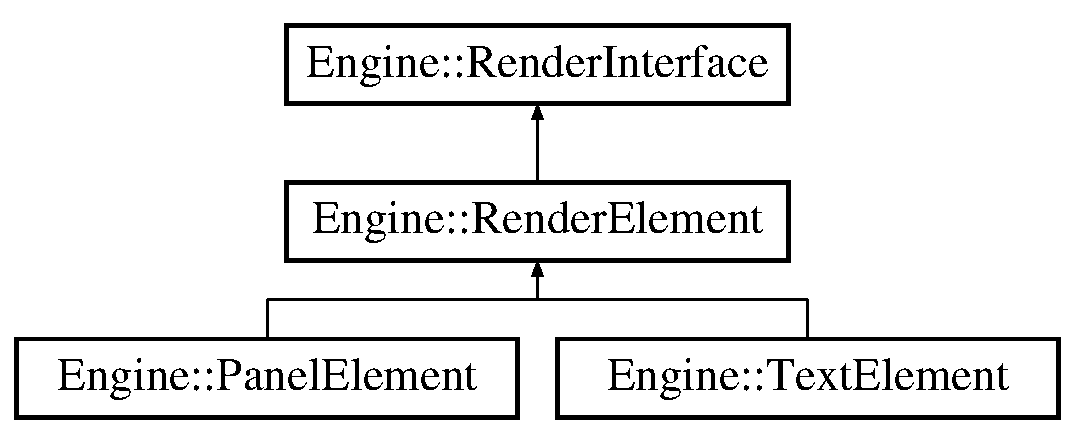
\includegraphics[height=3.000000cm]{classEngine_1_1RenderElement}
\end{center}
\end{figure}
\subsection*{Public Member Functions}
\begin{DoxyCompactItemize}
\item 
\hypertarget{classEngine_1_1RenderElement_adec31a17548437703c9cb8128e001ace}{}{\bfseries Render\+Element} (const std\+::string \&name)\label{classEngine_1_1RenderElement_adec31a17548437703c9cb8128e001ace}

\item 
\hypertarget{classEngine_1_1RenderElement_a885d6f55e3084a250f7ffec816166815}{}void {\bfseries set\+Element} (\hyperlink{classEngine_1_1Element}{Element} $\ast$element)\label{classEngine_1_1RenderElement_a885d6f55e3084a250f7ffec816166815}

\item 
\hypertarget{classEngine_1_1RenderElement_a5fb3b64eaadda98aeec7ca6ca0b9315c}{}\hyperlink{classEngine_1_1Element}{Element} $\ast$ {\bfseries get\+Element} (void)\label{classEngine_1_1RenderElement_a5fb3b64eaadda98aeec7ca6ca0b9315c}

\end{DoxyCompactItemize}
\subsection*{Protected Attributes}
\begin{DoxyCompactItemize}
\item 
\hypertarget{classEngine_1_1RenderElement_a11af48bd094c96669b1a030335986d67}{}\hyperlink{classEngine_1_1Element}{Element} $\ast$ {\bfseries m\+\_\+element}\label{classEngine_1_1RenderElement_a11af48bd094c96669b1a030335986d67}

\end{DoxyCompactItemize}


\subsection{Detailed Description}
The \hyperlink{classEngine_1_1RenderElement}{Render\+Element} -\/ contained component \hyperlink{classEngine_1_1Element}{Element} -\/ abstract class. 

The documentation for this class was generated from the following file\+:\begin{DoxyCompactItemize}
\item 
include/\+Interface/rendercomponent.\+h\end{DoxyCompactItemize}

\hypertarget{classEngine_1_1RenderEntity}{}\section{Engine\+:\+:Render\+Entity Class Reference}
\label{classEngine_1_1RenderEntity}\index{Engine\+::\+Render\+Entity@{Engine\+::\+Render\+Entity}}


The \hyperlink{classEngine_1_1RenderEntity}{Render\+Entity} -\/ contained component \hyperlink{classEngine_1_1Entity}{Entity} -\/ abstract class.  




{\ttfamily \#include $<$rendercomponent.\+h$>$}

Inheritance diagram for Engine\+:\+:Render\+Entity\+:\begin{figure}[H]
\begin{center}
\leavevmode
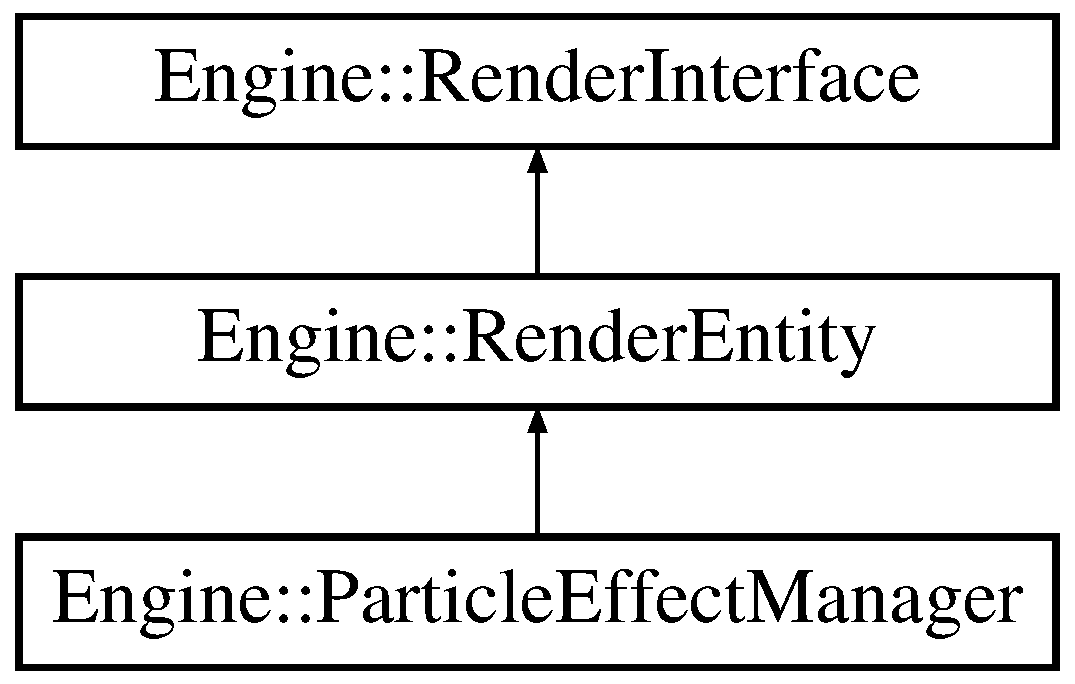
\includegraphics[height=3.000000cm]{classEngine_1_1RenderEntity}
\end{center}
\end{figure}
\subsection*{Public Member Functions}
\begin{DoxyCompactItemize}
\item 
\hypertarget{classEngine_1_1RenderEntity_a6db47242e2ed9f991b121f493db87f61}{}{\bfseries Render\+Entity} (const std\+::string \&name)\label{classEngine_1_1RenderEntity_a6db47242e2ed9f991b121f493db87f61}

\item 
\hypertarget{classEngine_1_1RenderEntity_a6a2857cacc97308800424731135df39d}{}void {\bfseries set\+Entity} (\hyperlink{classEngine_1_1Entity}{Entity} $\ast$entity)\label{classEngine_1_1RenderEntity_a6a2857cacc97308800424731135df39d}

\item 
\hypertarget{classEngine_1_1RenderEntity_af3aaf91fa4075bdd490e809650d06579}{}\hyperlink{classEngine_1_1Entity}{Entity} $\ast$ {\bfseries get\+Entity} (void)\label{classEngine_1_1RenderEntity_af3aaf91fa4075bdd490e809650d06579}

\end{DoxyCompactItemize}
\subsection*{Protected Attributes}
\begin{DoxyCompactItemize}
\item 
\hypertarget{classEngine_1_1RenderEntity_a42cd72f5efd42958dac5138d046a2d8d}{}\hyperlink{classEngine_1_1Entity}{Entity} $\ast$ {\bfseries m\+\_\+entity}\label{classEngine_1_1RenderEntity_a42cd72f5efd42958dac5138d046a2d8d}

\end{DoxyCompactItemize}


\subsection{Detailed Description}
The \hyperlink{classEngine_1_1RenderEntity}{Render\+Entity} -\/ contained component \hyperlink{classEngine_1_1Entity}{Entity} -\/ abstract class. 

The documentation for this class was generated from the following file\+:\begin{DoxyCompactItemize}
\item 
include/\+Interface/rendercomponent.\+h\end{DoxyCompactItemize}

\hypertarget{classEngine_1_1RenderEntityManager}{}\section{Engine\+:\+:Render\+Entity\+Manager Class Reference}
\label{classEngine_1_1RenderEntityManager}\index{Engine\+::\+Render\+Entity\+Manager@{Engine\+::\+Render\+Entity\+Manager}}
\subsection*{Public Member Functions}
\begin{DoxyCompactItemize}
\item 
\hypertarget{classEngine_1_1RenderEntityManager_aa31d822f8ddcc202d61af4433fc3ce84}{}void {\bfseries add\+Entity} (\hyperlink{classEngine_1_1RenderEntity}{Render\+Entity} $\ast$entity)\label{classEngine_1_1RenderEntityManager_aa31d822f8ddcc202d61af4433fc3ce84}

\item 
\hypertarget{classEngine_1_1RenderEntityManager_a2af97d37c0f503cbd99dbaa291364dc5}{}void {\bfseries remove} (\hyperlink{classEngine_1_1RenderEntity}{Render\+Entity} $\ast$entity)\label{classEngine_1_1RenderEntityManager_a2af97d37c0f503cbd99dbaa291364dc5}

\item 
\hypertarget{classEngine_1_1RenderEntityManager_afc0a2f61569fe06ba7c8176149c822b7}{}void {\bfseries Render\+All} (const \hyperlink{classEngine_1_1DrawEvent}{Draw\+Event} \&event)\label{classEngine_1_1RenderEntityManager_afc0a2f61569fe06ba7c8176149c822b7}

\item 
\hypertarget{classEngine_1_1RenderEntityManager_a2b11706d6b3932d1d1fdb0dc6415604a}{}Render\+Entity\+List {\bfseries get\+Entitys} (void)\label{classEngine_1_1RenderEntityManager_a2b11706d6b3932d1d1fdb0dc6415604a}

\end{DoxyCompactItemize}


The documentation for this class was generated from the following files\+:\begin{DoxyCompactItemize}
\item 
include/\+Manager/renderentitymanager.\+h\item 
Engine/\+Manager/Render\+Entity\+Manager.\+cpp\end{DoxyCompactItemize}

\hypertarget{classEngine_1_1RenderInterface}{}\section{Engine\+:\+:Render\+Interface Class Reference}
\label{classEngine_1_1RenderInterface}\index{Engine\+::\+Render\+Interface@{Engine\+::\+Render\+Interface}}


The \hyperlink{classEngine_1_1RenderInterface}{Render\+Interface} class.  




{\ttfamily \#include $<$rendercomponent.\+h$>$}

Inheritance diagram for Engine\+:\+:Render\+Interface\+:\begin{figure}[H]
\begin{center}
\leavevmode
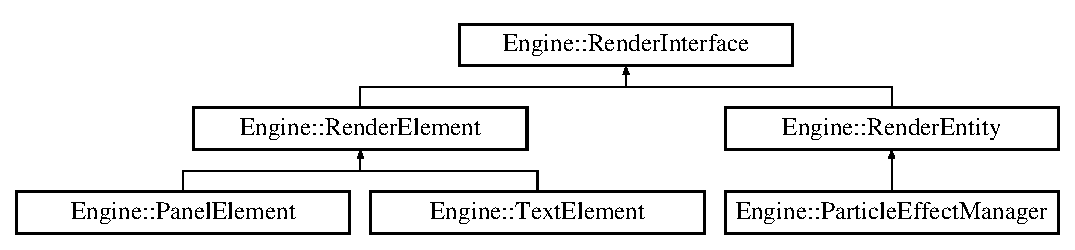
\includegraphics[height=2.916667cm]{classEngine_1_1RenderInterface}
\end{center}
\end{figure}
\subsection*{Public Member Functions}
\begin{DoxyCompactItemize}
\item 
\hypertarget{classEngine_1_1RenderInterface_ac5dac1a7783516383d82e5b0bccd60ff}{}virtual void {\bfseries create} (\hyperlink{classEngine_1_1OpenPolygonDisplay}{Open\+Polygon\+Display} $\ast$display)=0\label{classEngine_1_1RenderInterface_ac5dac1a7783516383d82e5b0bccd60ff}

\item 
\hypertarget{classEngine_1_1RenderInterface_abeb512e124483478198d354fafb38378}{}virtual void {\bfseries draw} (const \hyperlink{classEngine_1_1DrawEvent}{Draw\+Event} \&event)=0\label{classEngine_1_1RenderInterface_abeb512e124483478198d354fafb38378}

\end{DoxyCompactItemize}


\subsection{Detailed Description}
The \hyperlink{classEngine_1_1RenderInterface}{Render\+Interface} class. 

The documentation for this class was generated from the following file\+:\begin{DoxyCompactItemize}
\item 
include/\+Interface/rendercomponent.\+h\end{DoxyCompactItemize}

\hypertarget{classEngine_1_1RenderManager}{}\section{Engine\+:\+:Render\+Manager Class Reference}
\label{classEngine_1_1RenderManager}\index{Engine\+::\+Render\+Manager@{Engine\+::\+Render\+Manager}}


The \hyperlink{classEngine_1_1RenderManager}{Render\+Manager} class.  




{\ttfamily \#include $<$rendermanager.\+h$>$}

\subsection*{Public Member Functions}
\begin{DoxyCompactItemize}
\item 
\hypertarget{classEngine_1_1RenderManager_ac5745c80a5cc840117c033b0c82ccd67}{}void {\bfseries finish} (void)\label{classEngine_1_1RenderManager_ac5745c80a5cc840117c033b0c82ccd67}

\item 
\hypertarget{classEngine_1_1RenderManager_ab23d62cd43a7aa5aa86b70beeae0ee47}{}void {\bfseries set\+System\+Manager} (\hyperlink{classEngine_1_1SystemManager}{System\+Manager} $\ast$systemmanager)\label{classEngine_1_1RenderManager_ab23d62cd43a7aa5aa86b70beeae0ee47}

\item 
\hypertarget{classEngine_1_1RenderManager_a2a6d4a0f4d1c2fd00e079c2e68a5e17c}{}void {\bfseries set\+Tick\+Manager} (\hyperlink{classEngine_1_1TickManager}{Tick\+Manager} $\ast$tickmanager)\label{classEngine_1_1RenderManager_a2a6d4a0f4d1c2fd00e079c2e68a5e17c}

\item 
\hypertarget{classEngine_1_1RenderManager_a9732b4ce4ca97ce147af30da42623460}{}\hyperlink{classEngine_1_1SystemManager}{System\+Manager} $\ast$ {\bfseries get\+System\+Manager} (void)\label{classEngine_1_1RenderManager_a9732b4ce4ca97ce147af30da42623460}

\item 
\hypertarget{classEngine_1_1RenderManager_ae78f85dd1f25126e5a2f3da414b2b114}{}\hyperlink{classEngine_1_1TickManager}{Tick\+Manager} $\ast$ {\bfseries get\+Tick\+Manager} (void)\label{classEngine_1_1RenderManager_ae78f85dd1f25126e5a2f3da414b2b114}

\item 
void \hyperlink{classEngine_1_1RenderManager_a463e244d820df2c2df726780cd02a994}{add\+Frame\+Listener} (\hyperlink{classEngine_1_1FrameListener}{Frame\+Listener} $\ast$frame\+\_\+listener)
\begin{DoxyCompactList}\small\item\em add\+Frame\+Listener \end{DoxyCompactList}\item 
void \hyperlink{classEngine_1_1RenderManager_ad7b499716987b670c03889145f31de5a}{remove} (\hyperlink{classEngine_1_1FrameListener}{Frame\+Listener} $\ast$listener)
\begin{DoxyCompactList}\small\item\em remove \end{DoxyCompactList}\item 
void \hyperlink{classEngine_1_1RenderManager_a5cab7b1cabe975c0da11ca84496cbef7}{init\+Frame\+Listeners} (\hyperlink{classEngine_1_1OpenPolygonDisplay}{Open\+Polygon\+Display} $\ast$display)
\begin{DoxyCompactList}\small\item\em init\+Frame\+Listeners \end{DoxyCompactList}\item 
void \hyperlink{classEngine_1_1RenderManager_a245010f7acbd72c4c8e5b8cf11c2ffff}{Render\+Logic} (float time)
\begin{DoxyCompactList}\small\item\em Render\+Logic ( 1 / get\+L\+P\+S ) \end{DoxyCompactList}\item 
void \hyperlink{classEngine_1_1RenderManager_ad387f88864c0fb6815e59fd884ea8541}{Render\+Frame} (\hyperlink{classEngine_1_1OpenPolygonDisplay}{Open\+Polygon\+Display} $\ast$display)
\begin{DoxyCompactList}\small\item\em Render\+Frame. \end{DoxyCompactList}\end{DoxyCompactItemize}
\subsection*{Static Public Member Functions}
\begin{DoxyCompactItemize}
\item 
static \hyperlink{classEngine_1_1RenderManager}{Render\+Manager} $\ast$ \hyperlink{classEngine_1_1RenderManager_adb380605afe276a5b9afec04deab1bac}{get\+Singleton\+Ptr} (void)
\begin{DoxyCompactList}\small\item\em get\+Singleton\+Ptr \end{DoxyCompactList}\end{DoxyCompactItemize}


\subsection{Detailed Description}
The \hyperlink{classEngine_1_1RenderManager}{Render\+Manager} class. 

Management of Render\+Systems


\begin{DoxyItemize}
\item using actually one \hyperlink{classEngine_1_1RenderSystem}{Render\+System}
\item create one Display ( comming soon \hyperlink{classEngine_1_1DisplayManager}{Display\+Manager} )
\item add \hyperlink{classEngine_1_1FrameListener}{Frame\+Listener}
\item init \hyperlink{classEngine_1_1FrameListener}{Frame\+Listener}
\item trigger Render Logic
\item Render a single Frame
\item Design\+: Event , \hyperlink{classEngine_1_1Singleton}{Singleton} , Bridge 
\end{DoxyItemize}

\subsection{Member Function Documentation}
\hypertarget{classEngine_1_1RenderManager_a463e244d820df2c2df726780cd02a994}{}\index{Engine\+::\+Render\+Manager@{Engine\+::\+Render\+Manager}!add\+Frame\+Listener@{add\+Frame\+Listener}}
\index{add\+Frame\+Listener@{add\+Frame\+Listener}!Engine\+::\+Render\+Manager@{Engine\+::\+Render\+Manager}}
\subsubsection[{add\+Frame\+Listener(\+Frame\+Listener $\ast$frame\+\_\+listener)}]{\setlength{\rightskip}{0pt plus 5cm}void Render\+Manager\+::add\+Frame\+Listener (
\begin{DoxyParamCaption}
\item[{{\bf Frame\+Listener} $\ast$}]{frame\+\_\+listener}
\end{DoxyParamCaption}
)}\label{classEngine_1_1RenderManager_a463e244d820df2c2df726780cd02a994}


add\+Frame\+Listener 

Add Logic $\vert$ Frame Listener 
\begin{DoxyParams}{Parameters}
{\em frame\+\_\+listener} & \\
\hline
\end{DoxyParams}
\hypertarget{classEngine_1_1RenderManager_adb380605afe276a5b9afec04deab1bac}{}\index{Engine\+::\+Render\+Manager@{Engine\+::\+Render\+Manager}!get\+Singleton\+Ptr@{get\+Singleton\+Ptr}}
\index{get\+Singleton\+Ptr@{get\+Singleton\+Ptr}!Engine\+::\+Render\+Manager@{Engine\+::\+Render\+Manager}}
\subsubsection[{get\+Singleton\+Ptr(void)}]{\setlength{\rightskip}{0pt plus 5cm}Render\+Manager\+::get\+Singleton\+Ptr (
\begin{DoxyParamCaption}
\item[{void}]{}
\end{DoxyParamCaption}
)\hspace{0.3cm}{\ttfamily [static]}}\label{classEngine_1_1RenderManager_adb380605afe276a5b9afec04deab1bac}


get\+Singleton\+Ptr 

Return \hyperlink{classEngine_1_1RenderManager}{Render\+Manager} Instance \begin{DoxyReturn}{Returns}

\end{DoxyReturn}
\hypertarget{classEngine_1_1RenderManager_a5cab7b1cabe975c0da11ca84496cbef7}{}\index{Engine\+::\+Render\+Manager@{Engine\+::\+Render\+Manager}!init\+Frame\+Listeners@{init\+Frame\+Listeners}}
\index{init\+Frame\+Listeners@{init\+Frame\+Listeners}!Engine\+::\+Render\+Manager@{Engine\+::\+Render\+Manager}}
\subsubsection[{init\+Frame\+Listeners(\+Open\+Polygon\+Display $\ast$display)}]{\setlength{\rightskip}{0pt plus 5cm}void Render\+Manager\+::init\+Frame\+Listeners (
\begin{DoxyParamCaption}
\item[{{\bf Open\+Polygon\+Display} $\ast$}]{display}
\end{DoxyParamCaption}
)}\label{classEngine_1_1RenderManager_a5cab7b1cabe975c0da11ca84496cbef7}


init\+Frame\+Listeners 

Init Frame Listeners \hypertarget{classEngine_1_1RenderManager_ad7b499716987b670c03889145f31de5a}{}\index{Engine\+::\+Render\+Manager@{Engine\+::\+Render\+Manager}!remove@{remove}}
\index{remove@{remove}!Engine\+::\+Render\+Manager@{Engine\+::\+Render\+Manager}}
\subsubsection[{remove(\+Frame\+Listener $\ast$listener)}]{\setlength{\rightskip}{0pt plus 5cm}void Render\+Manager\+::remove (
\begin{DoxyParamCaption}
\item[{{\bf Frame\+Listener} $\ast$}]{listener}
\end{DoxyParamCaption}
)}\label{classEngine_1_1RenderManager_ad7b499716987b670c03889145f31de5a}


remove 

Remove Listener 
\begin{DoxyParams}{Parameters}
{\em listener} & \\
\hline
\end{DoxyParams}
\hypertarget{classEngine_1_1RenderManager_ad387f88864c0fb6815e59fd884ea8541}{}\index{Engine\+::\+Render\+Manager@{Engine\+::\+Render\+Manager}!Render\+Frame@{Render\+Frame}}
\index{Render\+Frame@{Render\+Frame}!Engine\+::\+Render\+Manager@{Engine\+::\+Render\+Manager}}
\subsubsection[{Render\+Frame(\+Open\+Polygon\+Display $\ast$display)}]{\setlength{\rightskip}{0pt plus 5cm}void Render\+Manager\+::\+Render\+Frame (
\begin{DoxyParamCaption}
\item[{{\bf Open\+Polygon\+Display} $\ast$}]{display}
\end{DoxyParamCaption}
)}\label{classEngine_1_1RenderManager_ad387f88864c0fb6815e59fd884ea8541}


Render\+Frame. 

Render a single frame \hypertarget{classEngine_1_1RenderManager_a245010f7acbd72c4c8e5b8cf11c2ffff}{}\index{Engine\+::\+Render\+Manager@{Engine\+::\+Render\+Manager}!Render\+Logic@{Render\+Logic}}
\index{Render\+Logic@{Render\+Logic}!Engine\+::\+Render\+Manager@{Engine\+::\+Render\+Manager}}
\subsubsection[{Render\+Logic(float time)}]{\setlength{\rightskip}{0pt plus 5cm}void Render\+Manager\+::\+Render\+Logic (
\begin{DoxyParamCaption}
\item[{float}]{time}
\end{DoxyParamCaption}
)}\label{classEngine_1_1RenderManager_a245010f7acbd72c4c8e5b8cf11c2ffff}


Render\+Logic ( 1 / get\+L\+P\+S ) 

Render Logic 
\begin{DoxyParams}{Parameters}
{\em time} & \\
\hline
\end{DoxyParams}


The documentation for this class was generated from the following files\+:\begin{DoxyCompactItemize}
\item 
include/\+Manager/rendermanager.\+h\item 
Engine/\+Manager/Render\+Manager.\+cpp\item 
main.\+cpp\end{DoxyCompactItemize}

\hypertarget{classEngine_1_1RenderModul}{}\section{Engine\+:\+:Render\+Modul Class Reference}
\label{classEngine_1_1RenderModul}\index{Engine\+::\+Render\+Modul@{Engine\+::\+Render\+Modul}}
Inheritance diagram for Engine\+:\+:Render\+Modul\+:\begin{figure}[H]
\begin{center}
\leavevmode
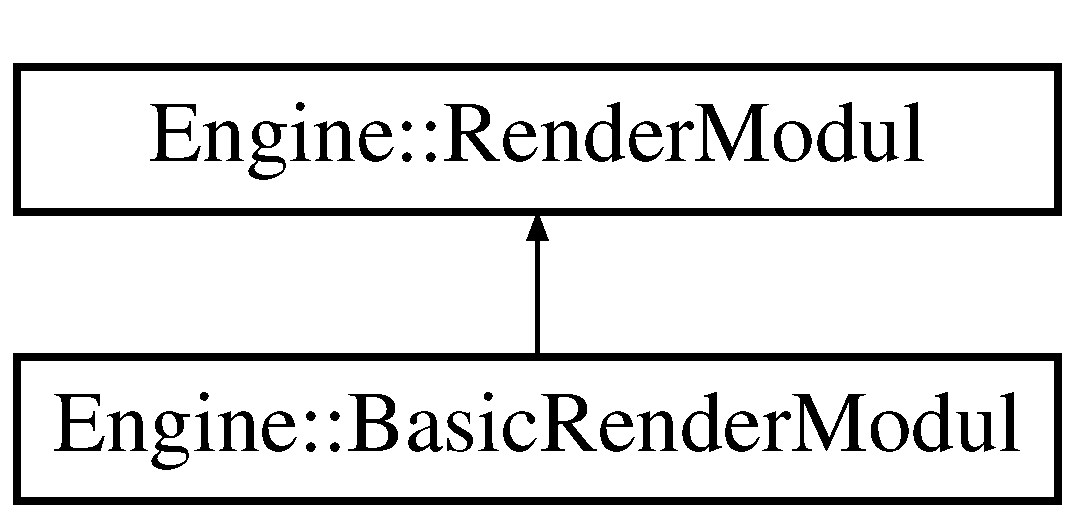
\includegraphics[height=2.000000cm]{classEngine_1_1RenderModul}
\end{center}
\end{figure}
\subsection*{Public Member Functions}
\begin{DoxyCompactItemize}
\item 
\hypertarget{classEngine_1_1RenderModul_a8e5e32ea29a067c49d7d855e589a7756}{}void {\bfseries set\+Render\+Entity\+Manager} (\hyperlink{classEngine_1_1RenderEntityManager}{Render\+Entity\+Manager} $\ast$render\+\_\+entity\+\_\+manager)\label{classEngine_1_1RenderModul_a8e5e32ea29a067c49d7d855e589a7756}

\item 
\hypertarget{classEngine_1_1RenderModul_ab943c038ae188d3d69af12a71525edef}{}virtual void {\bfseries render\+Process} (const \hyperlink{classEngine_1_1DrawEvent}{Draw\+Event} \&event)=0\label{classEngine_1_1RenderModul_ab943c038ae188d3d69af12a71525edef}

\item 
\hypertarget{classEngine_1_1RenderModul_a986b94ac3e33e30d470b425069644f42}{}\hyperlink{classEngine_1_1RenderEntityManager}{Render\+Entity\+Manager} $\ast$ {\bfseries get\+Render\+Entity\+Manager} (void)\label{classEngine_1_1RenderModul_a986b94ac3e33e30d470b425069644f42}

\end{DoxyCompactItemize}
\subsection*{Protected Attributes}
\begin{DoxyCompactItemize}
\item 
\hypertarget{classEngine_1_1RenderModul_aa471dc28208c160d1481980b0ab15b7e}{}\hyperlink{classEngine_1_1RenderEntityManager}{Render\+Entity\+Manager} $\ast$ {\bfseries m\+\_\+render\+\_\+entity\+\_\+manager}\label{classEngine_1_1RenderModul_aa471dc28208c160d1481980b0ab15b7e}

\end{DoxyCompactItemize}


The documentation for this class was generated from the following files\+:\begin{DoxyCompactItemize}
\item 
include/\+Render/\+Modul/rendermodul.\+h\item 
Engine/\+Render/\+Modul/Render\+Modul.\+cpp\end{DoxyCompactItemize}

\hypertarget{classEngine_1_1RenderModulManager}{}\section{Engine\+:\+:Render\+Modul\+Manager Class Reference}
\label{classEngine_1_1RenderModulManager}\index{Engine\+::\+Render\+Modul\+Manager@{Engine\+::\+Render\+Modul\+Manager}}
\subsection*{Public Member Functions}
\begin{DoxyCompactItemize}
\item 
\hypertarget{classEngine_1_1RenderModulManager_a44e24448e5ff4000310c2674e8cea047}{}void {\bfseries set\+Render\+Entity\+Manager} (\hyperlink{classEngine_1_1RenderEntityManager}{Render\+Entity\+Manager} $\ast$entity\+\_\+manager)\label{classEngine_1_1RenderModulManager_a44e24448e5ff4000310c2674e8cea047}

\item 
\hypertarget{classEngine_1_1RenderModulManager_a1ac160d546436a23eab7f23130b0dc53}{}void {\bfseries add\+Modul} (\hyperlink{classEngine_1_1RenderModul}{Render\+Modul} $\ast$modul, const std\+::string \&modul\+\_\+name)\label{classEngine_1_1RenderModulManager_a1ac160d546436a23eab7f23130b0dc53}

\item 
\hypertarget{classEngine_1_1RenderModulManager_aa37ce4d2ddcf621f538456251712c3ff}{}void {\bfseries remove} (\hyperlink{classEngine_1_1RenderModul}{Render\+Modul} $\ast$modul)\label{classEngine_1_1RenderModulManager_aa37ce4d2ddcf621f538456251712c3ff}

\item 
\hypertarget{classEngine_1_1RenderModulManager_ac8ac2e7e4b67de1dcc2d934ca63cdc07}{}Render\+Modul\+List {\bfseries get\+Modul\+List} (void)\label{classEngine_1_1RenderModulManager_ac8ac2e7e4b67de1dcc2d934ca63cdc07}

\end{DoxyCompactItemize}


The documentation for this class was generated from the following files\+:\begin{DoxyCompactItemize}
\item 
include/\+Manager/rendermodulmanager.\+h\item 
Engine/\+Manager/Render\+Modul\+Manager.\+cpp\end{DoxyCompactItemize}

\hypertarget{classEngine_1_1RenderProcessManager}{}\section{Engine\+:\+:Render\+Process\+Manager Class Reference}
\label{classEngine_1_1RenderProcessManager}\index{Engine\+::\+Render\+Process\+Manager@{Engine\+::\+Render\+Process\+Manager}}
\subsection*{Public Member Functions}
\begin{DoxyCompactItemize}
\item 
\hypertarget{classEngine_1_1RenderProcessManager_a48f095abe235bed49d5cb2e818efbfa0}{}{\bfseries Render\+Process\+Manager} (\hyperlink{classEngine_1_1RenderEntityManager}{Render\+Entity\+Manager} $\ast$entity\+\_\+manager)\label{classEngine_1_1RenderProcessManager_a48f095abe235bed49d5cb2e818efbfa0}

\item 
\hypertarget{classEngine_1_1RenderProcessManager_aa779a6d142e4538f229f9406a3d57d0b}{}void {\bfseries set\+Render\+Modul\+Manager} (\hyperlink{classEngine_1_1RenderModulManager}{Render\+Modul\+Manager} $\ast$modul\+\_\+manager)\label{classEngine_1_1RenderProcessManager_aa779a6d142e4538f229f9406a3d57d0b}

\item 
\hypertarget{classEngine_1_1RenderProcessManager_a3d84b0597479997b7932348368478bdf}{}void {\bfseries render\+Process} (const \hyperlink{classEngine_1_1DrawEvent}{Draw\+Event} \&event)\label{classEngine_1_1RenderProcessManager_a3d84b0597479997b7932348368478bdf}

\item 
\hypertarget{classEngine_1_1RenderProcessManager_aab5b64ca332db3abf712dfbe86933317}{}void {\bfseries render\+Classic\+Process} (const \hyperlink{classEngine_1_1DrawEvent}{Draw\+Event} \&event)\label{classEngine_1_1RenderProcessManager_aab5b64ca332db3abf712dfbe86933317}

\item 
\hypertarget{classEngine_1_1RenderProcessManager_a4519441f6f25368ab753b0c804fe708b}{}\hyperlink{classEngine_1_1RenderEntityManager}{Render\+Entity\+Manager} $\ast$ {\bfseries get\+Render\+Entity\+Manager} (void)\label{classEngine_1_1RenderProcessManager_a4519441f6f25368ab753b0c804fe708b}

\end{DoxyCompactItemize}


The documentation for this class was generated from the following files\+:\begin{DoxyCompactItemize}
\item 
include/\+Manager/renderprocessmanager.\+h\item 
Engine/\+Manager/Render\+Process\+Manager.\+cpp\end{DoxyCompactItemize}

\hypertarget{classEngine_1_1RenderSystem}{}\section{Engine\+:\+:Render\+System Class Reference}
\label{classEngine_1_1RenderSystem}\index{Engine\+::\+Render\+System@{Engine\+::\+Render\+System}}


The \hyperlink{classEngine_1_1RenderSystem}{Render\+System} -\/ abstract / interface class.  




{\ttfamily \#include $<$rendersystem.\+h$>$}

Inheritance diagram for Engine\+:\+:Render\+System\+:\begin{figure}[H]
\begin{center}
\leavevmode
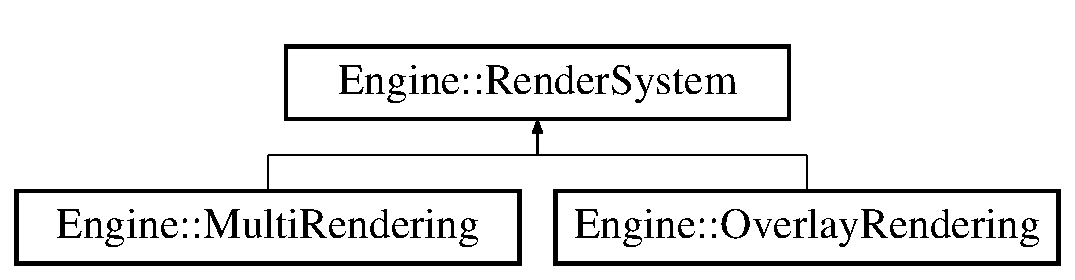
\includegraphics[height=2.000000cm]{classEngine_1_1RenderSystem}
\end{center}
\end{figure}
\subsection*{Public Member Functions}
\begin{DoxyCompactItemize}
\item 
\hypertarget{classEngine_1_1RenderSystem_a053d7789d0341adb6598fc9a96fd0d65}{}{\bfseries Render\+System} (const std\+::string \&system\+\_\+name)\label{classEngine_1_1RenderSystem_a053d7789d0341adb6598fc9a96fd0d65}

\item 
\hypertarget{classEngine_1_1RenderSystem_ab469fe67089be47101aede4cd8bd921f}{}virtual void {\bfseries initialize} (\hyperlink{classEngine_1_1OpenPolygonDisplay}{Open\+Polygon\+Display} $\ast$display)\label{classEngine_1_1RenderSystem_ab469fe67089be47101aede4cd8bd921f}

\item 
\hypertarget{classEngine_1_1RenderSystem_a13f2af110456c3bc78e26a9ebaf1cf49}{}virtual void {\bfseries Render\+Frame} (void)=0\label{classEngine_1_1RenderSystem_a13f2af110456c3bc78e26a9ebaf1cf49}

\item 
\hypertarget{classEngine_1_1RenderSystem_a2606351d12604c0a4c0ae93b71914234}{}virtual void {\bfseries Resize} (void)=0\label{classEngine_1_1RenderSystem_a2606351d12604c0a4c0ae93b71914234}

\item 
\hypertarget{classEngine_1_1RenderSystem_a7ad5563108b0d0cf20136e6f1adf6505}{}bool {\bfseries is\+Initialized} (void)\label{classEngine_1_1RenderSystem_a7ad5563108b0d0cf20136e6f1adf6505}

\item 
\hypertarget{classEngine_1_1RenderSystem_a846943fe6a49f2c5a5263020f10e1c87}{}void {\bfseries add\+Technique} (\hyperlink{classEngine_1_1Technique}{Technique} $\ast$technique)\label{classEngine_1_1RenderSystem_a846943fe6a49f2c5a5263020f10e1c87}

\item 
\hypertarget{classEngine_1_1RenderSystem_afbbcc6ff7c42f703f2f5296e9b424dd5}{}void {\bfseries set\+Render\+Process\+Manager} (\hyperlink{classEngine_1_1RenderProcessManager}{Render\+Process\+Manager} $\ast$manager)\label{classEngine_1_1RenderSystem_afbbcc6ff7c42f703f2f5296e9b424dd5}

\item 
\hypertarget{classEngine_1_1RenderSystem_abc8659466eadafd5d86408734f9ced56}{}\hyperlink{classEngine_1_1RenderProcessManager}{Render\+Process\+Manager} $\ast$ {\bfseries get\+Render\+Process\+Manager} (void)\label{classEngine_1_1RenderSystem_abc8659466eadafd5d86408734f9ced56}

\item 
\hypertarget{classEngine_1_1RenderSystem_ac20e2eac202e428d88b700ac25c4bdd5}{}\hyperlink{classEngine_1_1OpenPolygonDisplay}{Open\+Polygon\+Display} $\ast$ {\bfseries get\+Display} (void)\label{classEngine_1_1RenderSystem_ac20e2eac202e428d88b700ac25c4bdd5}

\end{DoxyCompactItemize}
\subsection*{Protected Attributes}
\begin{DoxyCompactItemize}
\item 
\hypertarget{classEngine_1_1RenderSystem_a69ecd8ab14e787d10dc32b53e1e21868}{}std\+::string {\bfseries m\+\_\+system\+\_\+name}\label{classEngine_1_1RenderSystem_a69ecd8ab14e787d10dc32b53e1e21868}

\item 
\hypertarget{classEngine_1_1RenderSystem_a45ae3752714b7333b2ad3e1497e7eb7a}{}glm\+::mat4 {\bfseries m\+\_\+projection}\label{classEngine_1_1RenderSystem_a45ae3752714b7333b2ad3e1497e7eb7a}

\item 
\hypertarget{classEngine_1_1RenderSystem_ab653743d56979f0e52f2b7a05285695f}{}glm\+::mat4 {\bfseries m\+\_\+ortho}\label{classEngine_1_1RenderSystem_ab653743d56979f0e52f2b7a05285695f}

\item 
\hypertarget{classEngine_1_1RenderSystem_afee785d4940eafb81af24cde5d611a0a}{}bool {\bfseries m\+\_\+init}\label{classEngine_1_1RenderSystem_afee785d4940eafb81af24cde5d611a0a}

\item 
\hypertarget{classEngine_1_1RenderSystem_ac45b3777921d3be67415b49e84e1a016}{}\hyperlink{classEngine_1_1OpenPolygonDisplay}{Open\+Polygon\+Display} $\ast$ {\bfseries m\+\_\+display}\label{classEngine_1_1RenderSystem_ac45b3777921d3be67415b49e84e1a016}

\item 
\hypertarget{classEngine_1_1RenderSystem_ac94142989e64db062909010d63e36ff8}{}\hyperlink{classEngine_1_1Camera}{Camera} $\ast$ {\bfseries m\+\_\+camera}\label{classEngine_1_1RenderSystem_ac94142989e64db062909010d63e36ff8}

\item 
\hypertarget{classEngine_1_1RenderSystem_a806926442339c805a0a277382c09602c}{}\hyperlink{classEngine_1_1RenderProcessManager}{Render\+Process\+Manager} $\ast$ {\bfseries m\+\_\+render\+\_\+process\+\_\+manager}\label{classEngine_1_1RenderSystem_a806926442339c805a0a277382c09602c}

\item 
\hypertarget{classEngine_1_1RenderSystem_a5617269e8b9b814bf6e92b3fc3374258}{}Techniques {\bfseries m\+\_\+techniques}\label{classEngine_1_1RenderSystem_a5617269e8b9b814bf6e92b3fc3374258}

\end{DoxyCompactItemize}


\subsection{Detailed Description}
The \hyperlink{classEngine_1_1RenderSystem}{Render\+System} -\/ abstract / interface class. 

The documentation for this class was generated from the following files\+:\begin{DoxyCompactItemize}
\item 
include/\+Render/rendersystem.\+h\item 
Engine/\+Render/Render\+System.\+cpp\end{DoxyCompactItemize}

\hypertarget{classEngine_1_1Shader}{}\section{Engine\+:\+:Shader Class Reference}
\label{classEngine_1_1Shader}\index{Engine\+::\+Shader@{Engine\+::\+Shader}}


The \hyperlink{classEngine_1_1Shader}{Shader} class.  




{\ttfamily \#include $<$shader.\+h$>$}

Inheritance diagram for Engine\+:\+:Shader\+:\begin{figure}[H]
\begin{center}
\leavevmode
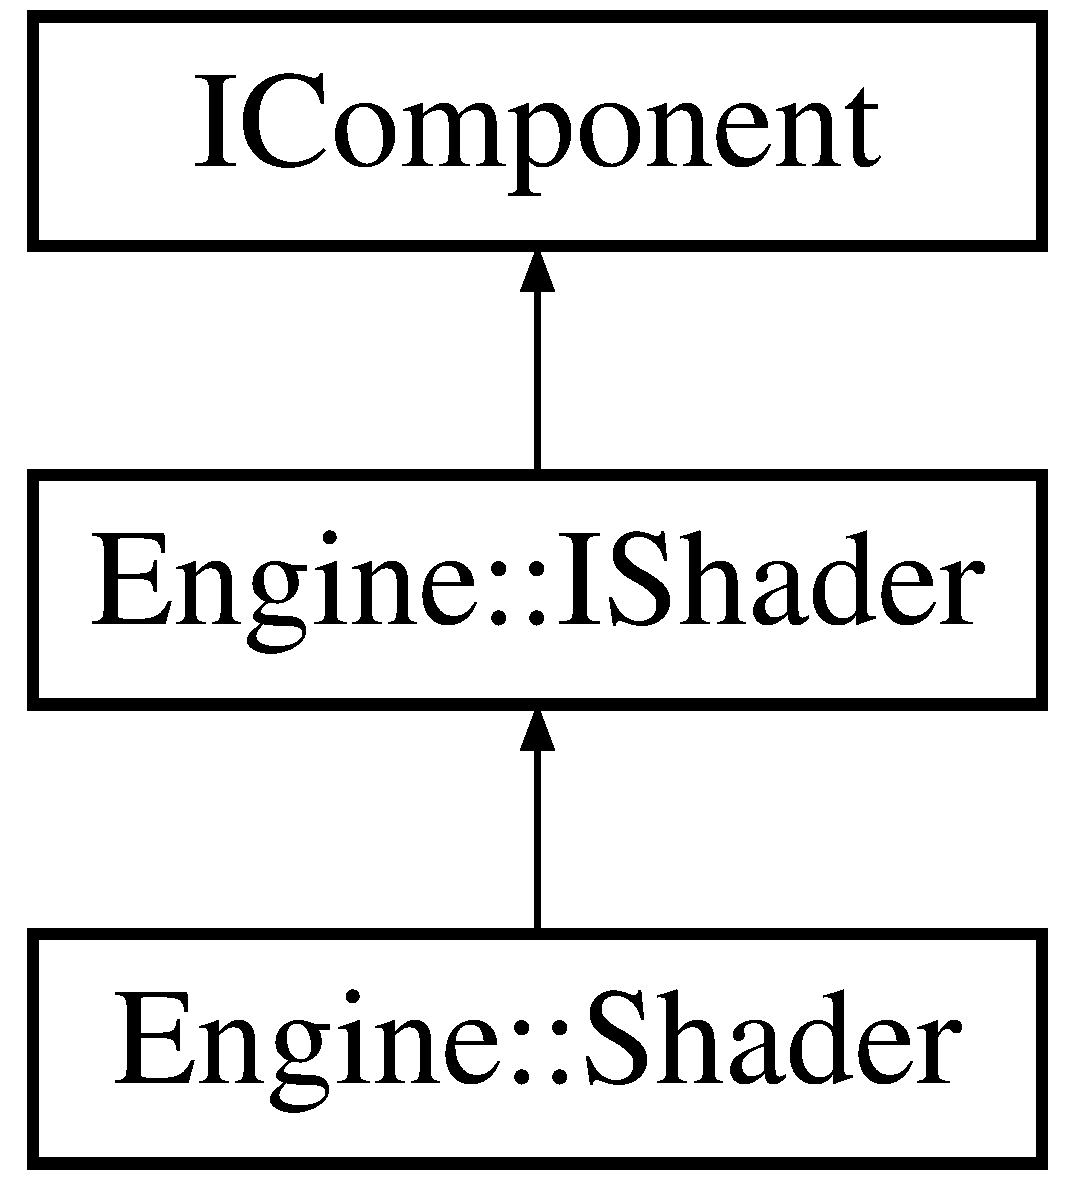
\includegraphics[height=3.000000cm]{classEngine_1_1Shader}
\end{center}
\end{figure}
\subsection*{Public Member Functions}
\begin{DoxyCompactItemize}
\item 
\hypertarget{classEngine_1_1Shader_a2ab3adc85f5ac7ed66669de0d5149ecf}{}void {\bfseries Use\+Program} (void)\label{classEngine_1_1Shader_a2ab3adc85f5ac7ed66669de0d5149ecf}

\item 
\hypertarget{classEngine_1_1Shader_a465a1bcbcefb47cda4715568891df59a}{}void {\bfseries Unused} (void)\label{classEngine_1_1Shader_a465a1bcbcefb47cda4715568891df59a}

\item 
\hypertarget{classEngine_1_1Shader_a42208d67fd98e68f945b7e26c7dbfbfb}{}void {\bfseries Link\+Program} (void)\label{classEngine_1_1Shader_a42208d67fd98e68f945b7e26c7dbfbfb}

\item 
\hypertarget{classEngine_1_1Shader_aac32f590f7f66dac5756bcc984e626c2}{}void {\bfseries Attach\+Shader} (uint shader)\label{classEngine_1_1Shader_aac32f590f7f66dac5756bcc984e626c2}

\item 
\hypertarget{classEngine_1_1Shader_a631c94b25466fce916cdfab0712809ef}{}void {\bfseries Bind\+Uniform1f} (const char $\ast$location, float number)\label{classEngine_1_1Shader_a631c94b25466fce916cdfab0712809ef}

\item 
\hypertarget{classEngine_1_1Shader_a866635c4c746bfb3dd1f4ce176871f0d}{}void {\bfseries Bind\+Uniform1i} (const char $\ast$location, int number)\label{classEngine_1_1Shader_a866635c4c746bfb3dd1f4ce176871f0d}

\item 
\hypertarget{classEngine_1_1Shader_a05147be1958f68d9eda10ff3bee24361}{}void {\bfseries Bind\+Matrix} (const char $\ast$location, glm\+::mat4 matrix)\label{classEngine_1_1Shader_a05147be1958f68d9eda10ff3bee24361}

\item 
\hypertarget{classEngine_1_1Shader_a0062df7c82a1be7bff14c8cb2010fde9}{}void {\bfseries Bind\+Vec3f} (const char $\ast$location, const \hyperlink{classVector3}{Vector3f} \&vector)\label{classEngine_1_1Shader_a0062df7c82a1be7bff14c8cb2010fde9}

\item 
\hypertarget{classEngine_1_1Shader_a565ae6adf7661c1da3acebbcee5ff97b}{}void {\bfseries Bind\+Vec3i} (const char $\ast$location, const \hyperlink{classVector3}{Vector3i} \&vector)\label{classEngine_1_1Shader_a565ae6adf7661c1da3acebbcee5ff97b}

\item 
\hypertarget{classEngine_1_1Shader_a5d999cd1952e19ff2ba31f9398195ceb}{}void {\bfseries Bind\+Vec4f} (const char $\ast$location, const \hyperlink{classVector4}{Vector4f} \&vector)\label{classEngine_1_1Shader_a5d999cd1952e19ff2ba31f9398195ceb}

\item 
\hypertarget{classEngine_1_1Shader_ad892a7e61b6556741fb6704076e8f806}{}void {\bfseries Bind\+Vec4i} (const char $\ast$location, const \hyperlink{classVector4}{Vector4i} \&vector)\label{classEngine_1_1Shader_ad892a7e61b6556741fb6704076e8f806}

\item 
\hypertarget{classEngine_1_1Shader_ae1e0209d240df2b89f34ec9e676c1209}{}void {\bfseries Bind\+Texture} (\hyperlink{classEngine_1_1Texture}{Texture} $\ast$texture, const char $\ast$location, int texture\+\_\+unit)\label{classEngine_1_1Shader_ae1e0209d240df2b89f34ec9e676c1209}

\item 
\hypertarget{classEngine_1_1Shader_a91c06a793941a96343674ab2fe4601d0}{}void {\bfseries Bind\+Attribute\+Location} (const char $\ast$location, int attribute\+\_\+id)\label{classEngine_1_1Shader_a91c06a793941a96343674ab2fe4601d0}

\item 
\hypertarget{classEngine_1_1Shader_a3f3967c2977707a1b3c53a1d498480cf}{}void {\bfseries Bind\+Frag\+Data} (const char $\ast$location, int frag\+\_\+position)\label{classEngine_1_1Shader_a3f3967c2977707a1b3c53a1d498480cf}

\end{DoxyCompactItemize}
\subsection*{Additional Inherited Members}


\subsection{Detailed Description}
The \hyperlink{classEngine_1_1Shader}{Shader} class. 

The documentation for this class was generated from the following files\+:\begin{DoxyCompactItemize}
\item 
include/\+Container/shader.\+h\item 
Container/Shader.\+cpp\end{DoxyCompactItemize}

\hypertarget{classEngine_1_1ShaderARB}{}\section{Engine\+:\+:Shader\+A\+R\+B Class Reference}
\label{classEngine_1_1ShaderARB}\index{Engine\+::\+Shader\+A\+R\+B@{Engine\+::\+Shader\+A\+R\+B}}


The \hyperlink{classEngine_1_1ShaderARB}{Shader\+A\+R\+B} class.  




{\ttfamily \#include $<$shaderarb.\+h$>$}

Inheritance diagram for Engine\+:\+:Shader\+A\+R\+B\+:\begin{figure}[H]
\begin{center}
\leavevmode
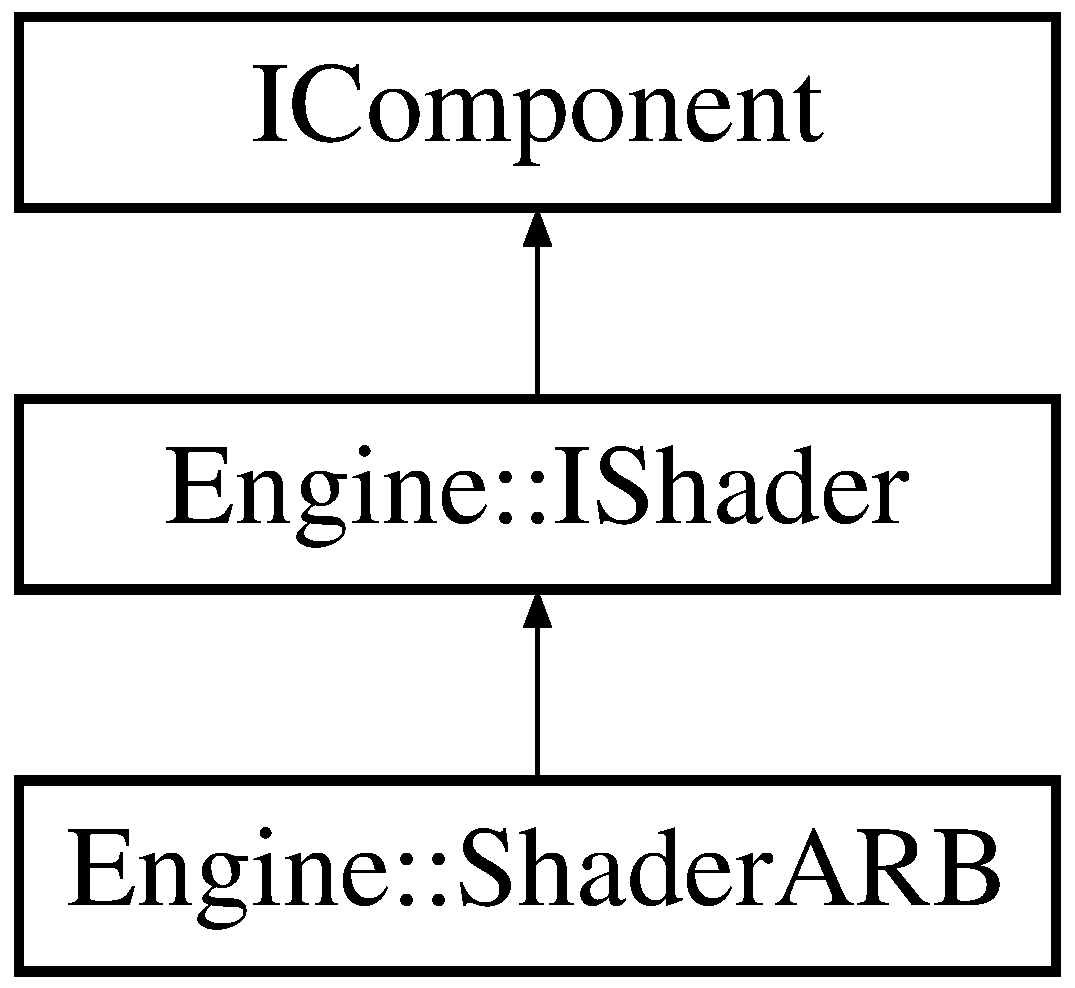
\includegraphics[height=3.000000cm]{classEngine_1_1ShaderARB}
\end{center}
\end{figure}
\subsection*{Public Member Functions}
\begin{DoxyCompactItemize}
\item 
\hypertarget{classEngine_1_1ShaderARB_a06f2725524cdf78189b30bc88459d1aa}{}void {\bfseries Use\+Program} (void)\label{classEngine_1_1ShaderARB_a06f2725524cdf78189b30bc88459d1aa}

\item 
\hypertarget{classEngine_1_1ShaderARB_a153d4e3d6499f118074c3ab48b3a91aa}{}void {\bfseries Unused} (void)\label{classEngine_1_1ShaderARB_a153d4e3d6499f118074c3ab48b3a91aa}

\item 
\hypertarget{classEngine_1_1ShaderARB_a76d4c923f44e56f052cd956eaadea4a0}{}void {\bfseries Link\+Program} (void)\label{classEngine_1_1ShaderARB_a76d4c923f44e56f052cd956eaadea4a0}

\item 
\hypertarget{classEngine_1_1ShaderARB_a162938b504280bf2073038b968ce142b}{}void {\bfseries Attach\+Shader} (uint shader)\label{classEngine_1_1ShaderARB_a162938b504280bf2073038b968ce142b}

\item 
\hypertarget{classEngine_1_1ShaderARB_afbd7960f5a877c6ae1fc6a201b593398}{}void {\bfseries Bind\+Uniform1f} (const char $\ast$location, float number)\label{classEngine_1_1ShaderARB_afbd7960f5a877c6ae1fc6a201b593398}

\item 
\hypertarget{classEngine_1_1ShaderARB_ab1b96ff776f8f049e0afe379e7c39ad6}{}void {\bfseries Bind\+Uniform1i} (const char $\ast$location, int number)\label{classEngine_1_1ShaderARB_ab1b96ff776f8f049e0afe379e7c39ad6}

\item 
\hypertarget{classEngine_1_1ShaderARB_a50d15a0d31d9d96c0364f69a3f033663}{}void {\bfseries Bind\+Matrix} (const char $\ast$location, glm\+::mat4 matrix)\label{classEngine_1_1ShaderARB_a50d15a0d31d9d96c0364f69a3f033663}

\item 
\hypertarget{classEngine_1_1ShaderARB_a51a4324f4f680038ec6edade070e65b0}{}void {\bfseries Bind\+Vec3f} (const char $\ast$location, const \hyperlink{classVector3}{Vector3f} \&vector)\label{classEngine_1_1ShaderARB_a51a4324f4f680038ec6edade070e65b0}

\item 
\hypertarget{classEngine_1_1ShaderARB_adf8f26bbc4817853fb5722b197679aaf}{}void {\bfseries Bind\+Vec3i} (const char $\ast$location, const \hyperlink{classVector3}{Vector3i} \&vector)\label{classEngine_1_1ShaderARB_adf8f26bbc4817853fb5722b197679aaf}

\item 
\hypertarget{classEngine_1_1ShaderARB_aaeafcdfa69b123c0f9b102b8f6c3b84e}{}void {\bfseries Bind\+Vec4f} (const char $\ast$location, const \hyperlink{classVector4}{Vector4f} \&vector)\label{classEngine_1_1ShaderARB_aaeafcdfa69b123c0f9b102b8f6c3b84e}

\item 
\hypertarget{classEngine_1_1ShaderARB_a02d657c199f2234b3d159ea117869b9d}{}void {\bfseries Bind\+Vec4i} (const char $\ast$location, const \hyperlink{classVector4}{Vector4i} \&vector)\label{classEngine_1_1ShaderARB_a02d657c199f2234b3d159ea117869b9d}

\item 
\hypertarget{classEngine_1_1ShaderARB_a8cca6a5db67fef72017c997a183f0aa7}{}void {\bfseries Bind\+Texture} (\hyperlink{classEngine_1_1Texture}{Texture} $\ast$texture, const char $\ast$location, int texture\+\_\+unit)\label{classEngine_1_1ShaderARB_a8cca6a5db67fef72017c997a183f0aa7}

\item 
\hypertarget{classEngine_1_1ShaderARB_a74be172310f19f7c243c6a0eab53bb9b}{}void {\bfseries Bind\+Attribute\+Location} (const char $\ast$location, int attribute\+\_\+id)\label{classEngine_1_1ShaderARB_a74be172310f19f7c243c6a0eab53bb9b}

\item 
\hypertarget{classEngine_1_1ShaderARB_a98f13df024cd7ab779fdc9c1c6e1267a}{}void {\bfseries Bind\+Frag\+Data} (const char $\ast$location, int frag\+\_\+position)\label{classEngine_1_1ShaderARB_a98f13df024cd7ab779fdc9c1c6e1267a}

\end{DoxyCompactItemize}
\subsection*{Additional Inherited Members}


\subsection{Detailed Description}
The \hyperlink{classEngine_1_1ShaderARB}{Shader\+A\+R\+B} class. 

The documentation for this class was generated from the following files\+:\begin{DoxyCompactItemize}
\item 
include/\+Container/shaderarb.\+h\item 
Container/Shader\+A\+R\+B.\+cpp\end{DoxyCompactItemize}

\hypertarget{classEngine_1_1ShaderManager}{}\section{Engine\+:\+:Shader\+Manager Class Reference}
\label{classEngine_1_1ShaderManager}\index{Engine\+::\+Shader\+Manager@{Engine\+::\+Shader\+Manager}}


The \hyperlink{classEngine_1_1ShaderManager}{Shader\+Manager} controlled \hyperlink{classEngine_1_1IShader}{I\+Shader} ( \hyperlink{classEngine_1_1Shader}{Shader} , \hyperlink{classEngine_1_1ShaderARB}{Shader\+A\+R\+B} )  




{\ttfamily \#include $<$shadermanager.\+h$>$}

Inheritance diagram for Engine\+:\+:Shader\+Manager\+:\begin{figure}[H]
\begin{center}
\leavevmode
\includegraphics[height=2.000000cm]{classEngine_1_1ShaderManager}
\end{center}
\end{figure}
\subsection*{Public Member Functions}
\begin{DoxyCompactItemize}
\item 
\hyperlink{classEngine_1_1IShader}{I\+Shader} $\ast$ \hyperlink{classEngine_1_1ShaderManager_a04436b2e5d1450b5d4828f121ad62b59}{create\+Shader} (const std\+::string \&shader\+\_\+name)
\begin{DoxyCompactList}\small\item\em create\+Shader \end{DoxyCompactList}\item 
\hypertarget{classEngine_1_1ShaderManager_aff321723a3ee2895d14efa5f9a1fb970}{}\hyperlink{classEngine_1_1IShader}{I\+Shader} $\ast$ {\bfseries create\+Shader\+A\+R\+B} (const std\+::string \&shader\+\_\+name)\label{classEngine_1_1ShaderManager_aff321723a3ee2895d14efa5f9a1fb970}

\item 
void \hyperlink{classEngine_1_1ShaderManager_a840d6840451cb9b191a4f0c0ad84854f}{add\+Source} (\hyperlink{classEngine_1_1IShader}{I\+Shader} $\ast$shader, const std\+::string \&shader\+\_\+file, uint shader\+\_\+types)
\begin{DoxyCompactList}\small\item\em add\+Source \end{DoxyCompactList}\item 
\hypertarget{classEngine_1_1ShaderManager_aef42d44027ae53273a6fcae937793630}{}void {\bfseries add\+Source\+A\+R\+B} (\hyperlink{classEngine_1_1IShader}{I\+Shader} $\ast$shader, const std\+::string \&shader\+\_\+file, uint shader\+\_\+types)\label{classEngine_1_1ShaderManager_aef42d44027ae53273a6fcae937793630}

\item 
\hypertarget{classEngine_1_1ShaderManager_a37df04871c43bca6c2899d0e6ae9b509}{}void {\bfseries add\+Embedded\+Source} (\hyperlink{classEngine_1_1IShader}{I\+Shader} $\ast$shader, const std\+::string \&name, const std\+::string \&source, uint shader\+\_\+types)\label{classEngine_1_1ShaderManager_a37df04871c43bca6c2899d0e6ae9b509}

\item 
\hyperlink{classEngine_1_1IShader}{I\+Shader} $\ast$ \hyperlink{classEngine_1_1ShaderManager_a5248b6515e8a50eb89375985289baf64}{get\+Shader} (uint container\+\_\+id)
\begin{DoxyCompactList}\small\item\em get\+Shader \end{DoxyCompactList}\item 
\hypertarget{classEngine_1_1ShaderManager_a64641685923c88f3356da1cd1e8f9d20}{}void {\bfseries destroy} (uint container\+\_\+id)\label{classEngine_1_1ShaderManager_a64641685923c88f3356da1cd1e8f9d20}

\item 
\hypertarget{classEngine_1_1ShaderManager_af80799a6e091b951195979300ef331d3}{}void {\bfseries get\+Program\+Error\+A\+R\+B} (uint program, const std\+::string \&information)\label{classEngine_1_1ShaderManager_af80799a6e091b951195979300ef331d3}

\item 
\hypertarget{classEngine_1_1ShaderManager_ac1ee62e48600af2bf3873f1fa0d4dc0a}{}void {\bfseries get\+Program\+Error} (uint program, const std\+::string \&information)\label{classEngine_1_1ShaderManager_ac1ee62e48600af2bf3873f1fa0d4dc0a}

\item 
\hypertarget{classEngine_1_1ShaderManager_a9f601072a850635d25c33ef0b724c876}{}void {\bfseries get\+Shader\+Error} (uint shader, const std\+::string \&information)\label{classEngine_1_1ShaderManager_a9f601072a850635d25c33ef0b724c876}

\item 
\hypertarget{classEngine_1_1ShaderManager_a1ff6cadd12a4d63624baf15aa4c2ab7f}{}std\+::string {\bfseries Load\+Shader} (const string \&file\+Name)\label{classEngine_1_1ShaderManager_a1ff6cadd12a4d63624baf15aa4c2ab7f}

\item 
\hypertarget{classEngine_1_1ShaderManager_a488ee4fd5e8e12130b0f39ac14b34747}{}uint {\bfseries Create\+Shader} (const std\+::string \&name, const string \&text, uint type)\label{classEngine_1_1ShaderManager_a488ee4fd5e8e12130b0f39ac14b34747}

\item 
\hypertarget{classEngine_1_1ShaderManager_a9eafba65e127c7c0f13135e3a36a9504}{}uint {\bfseries Create\+Shader\+A\+R\+B} (const std\+::string \&name, const string \&text, uint type)\label{classEngine_1_1ShaderManager_a9eafba65e127c7c0f13135e3a36a9504}

\item 
\hypertarget{classEngine_1_1ShaderManager_a907eb8f7b29905794d45747b8e4c5fbe}{}uint {\bfseries create\+Shader\+Type} (const string \&shader\+\_\+file, const string extension, uint shader\+\_\+type)\label{classEngine_1_1ShaderManager_a907eb8f7b29905794d45747b8e4c5fbe}

\item 
\hypertarget{classEngine_1_1ShaderManager_ac3cfdfc83bf97698d70fb51b5b1e0252}{}uint {\bfseries create\+Shader\+Type\+A\+R\+B} (const string \&shader\+\_\+file, const string extension, uint shader\+\_\+type)\label{classEngine_1_1ShaderManager_ac3cfdfc83bf97698d70fb51b5b1e0252}

\end{DoxyCompactItemize}


\subsection{Detailed Description}
The \hyperlink{classEngine_1_1ShaderManager}{Shader\+Manager} controlled \hyperlink{classEngine_1_1IShader}{I\+Shader} ( \hyperlink{classEngine_1_1Shader}{Shader} , \hyperlink{classEngine_1_1ShaderARB}{Shader\+A\+R\+B} ) 

Management of Shaders


\begin{DoxyItemize}
\item support only Open\+G\+L \hyperlink{classEngine_1_1Shader}{Shader} ( G\+L\+S\+L )
\item create \hyperlink{classEngine_1_1Shader}{Shader} with \hyperlink{classEngine_1_1Attribute}{Attribute} Locations 
\end{DoxyItemize}

\subsection{Member Function Documentation}
\hypertarget{classEngine_1_1ShaderManager_a840d6840451cb9b191a4f0c0ad84854f}{}\index{Engine\+::\+Shader\+Manager@{Engine\+::\+Shader\+Manager}!add\+Source@{add\+Source}}
\index{add\+Source@{add\+Source}!Engine\+::\+Shader\+Manager@{Engine\+::\+Shader\+Manager}}
\subsubsection[{add\+Source(\+I\+Shader $\ast$shader, const std\+::string \&shader\+\_\+file, uint shader\+\_\+types)}]{\setlength{\rightskip}{0pt plus 5cm}void Shader\+Manager\+::add\+Source (
\begin{DoxyParamCaption}
\item[{{\bf I\+Shader} $\ast$}]{shader, }
\item[{const std\+::string \&}]{shader\+\_\+file, }
\item[{uint}]{shader\+\_\+types}
\end{DoxyParamCaption}
)}\label{classEngine_1_1ShaderManager_a840d6840451cb9b191a4f0c0ad84854f}


add\+Source 

Add Source to \hyperlink{classEngine_1_1Shader}{Shader} 
\begin{DoxyParams}{Parameters}
{\em empty\+\_\+shader} & \+: empty \hyperlink{classEngine_1_1Shader}{Shader} ptr \\
\hline
{\em shader\+\_\+file} & \+: shader\+\_\+file ( source ) \\
\hline
{\em shader\+\_\+name} & \+: shader\+\_\+ \\
\hline
{\em flags} & \\
\hline
\end{DoxyParams}
\hypertarget{classEngine_1_1ShaderManager_a04436b2e5d1450b5d4828f121ad62b59}{}\index{Engine\+::\+Shader\+Manager@{Engine\+::\+Shader\+Manager}!create\+Shader@{create\+Shader}}
\index{create\+Shader@{create\+Shader}!Engine\+::\+Shader\+Manager@{Engine\+::\+Shader\+Manager}}
\subsubsection[{create\+Shader(const std\+::string \&shader\+\_\+name)}]{\setlength{\rightskip}{0pt plus 5cm}{\bf I\+Shader} $\ast$ Shader\+Manager\+::create\+Shader (
\begin{DoxyParamCaption}
\item[{const std\+::string \&}]{shader\+\_\+name}
\end{DoxyParamCaption}
)}\label{classEngine_1_1ShaderManager_a04436b2e5d1450b5d4828f121ad62b59}


create\+Shader 

Create a \hyperlink{classEngine_1_1Shader}{Shader} 
\begin{DoxyParams}{Parameters}
{\em shader\+\_\+name} & \\
\hline
\end{DoxyParams}
\begin{DoxyReturn}{Returns}

\end{DoxyReturn}
\hypertarget{classEngine_1_1ShaderManager_a5248b6515e8a50eb89375985289baf64}{}\index{Engine\+::\+Shader\+Manager@{Engine\+::\+Shader\+Manager}!get\+Shader@{get\+Shader}}
\index{get\+Shader@{get\+Shader}!Engine\+::\+Shader\+Manager@{Engine\+::\+Shader\+Manager}}
\subsubsection[{get\+Shader(uint container\+\_\+id)}]{\setlength{\rightskip}{0pt plus 5cm}{\bf I\+Shader} $\ast$ Shader\+Manager\+::get\+Shader (
\begin{DoxyParamCaption}
\item[{uint}]{container\+\_\+id}
\end{DoxyParamCaption}
)}\label{classEngine_1_1ShaderManager_a5248b6515e8a50eb89375985289baf64}


get\+Shader 

Return \hyperlink{classEngine_1_1Shader}{Shader} Object by component id or shader name 
\begin{DoxyParams}{Parameters}
{\em component\+\_\+id} & \\
\hline
\end{DoxyParams}
\begin{DoxyReturn}{Returns}

\end{DoxyReturn}


The documentation for this class was generated from the following files\+:\begin{DoxyCompactItemize}
\item 
include/\+Manager/shadermanager.\+h\item 
Engine/\+Manager/Shader\+Manager.\+cpp\end{DoxyCompactItemize}

\hypertarget{classEngine_1_1ShadowEvent}{}\section{Engine\+:\+:Shadow\+Event Class Reference}
\label{classEngine_1_1ShadowEvent}\index{Engine\+::\+Shadow\+Event@{Engine\+::\+Shadow\+Event}}


The \hyperlink{classEngine_1_1ShadowEvent}{Shadow\+Event} -\/ Event class.  




{\ttfamily \#include $<$shadowevent.\+h$>$}

\subsection*{Public Member Functions}
\begin{DoxyCompactItemize}
\item 
\hypertarget{classEngine_1_1ShadowEvent_a795be7aa3f4d33f92ca53a58b5a3cf5b}{}void {\bfseries set\+Projection} (glm\+::mat4 projection\+\_\+matrix)\label{classEngine_1_1ShadowEvent_a795be7aa3f4d33f92ca53a58b5a3cf5b}

\item 
\hypertarget{classEngine_1_1ShadowEvent_ad4630998cafa554cd941824e745b03b6}{}void {\bfseries set\+Matrix} (glm\+::mat4 shadow\+\_\+view\+\_\+matrix)\label{classEngine_1_1ShadowEvent_ad4630998cafa554cd941824e745b03b6}

\item 
\hypertarget{classEngine_1_1ShadowEvent_ac2f0d9b1cb444a7c0dfea5b767c6776f}{}void {\bfseries set\+Shadow\+Shader} (\hyperlink{classEngine_1_1IShader}{I\+Shader} $\ast$shader)\label{classEngine_1_1ShadowEvent_ac2f0d9b1cb444a7c0dfea5b767c6776f}

\item 
\hypertarget{classEngine_1_1ShadowEvent_a9f2a5cc88e939acfada62435c3b63eb6}{}\hyperlink{classEngine_1_1IShader}{I\+Shader} $\ast$ {\bfseries get\+Shadow\+Shader} (void) const \label{classEngine_1_1ShadowEvent_a9f2a5cc88e939acfada62435c3b63eb6}

\item 
\hypertarget{classEngine_1_1ShadowEvent_a0b0838ac90dce47bbdedcb2334a44462}{}glm\+::mat4 {\bfseries get\+View\+Matrix} (void) const \label{classEngine_1_1ShadowEvent_a0b0838ac90dce47bbdedcb2334a44462}

\item 
\hypertarget{classEngine_1_1ShadowEvent_aceb75064aaab60a83af77155b18c2e89}{}glm\+::mat4 {\bfseries get\+Projection} (void) const \label{classEngine_1_1ShadowEvent_aceb75064aaab60a83af77155b18c2e89}

\end{DoxyCompactItemize}


\subsection{Detailed Description}
The \hyperlink{classEngine_1_1ShadowEvent}{Shadow\+Event} -\/ Event class. 

The documentation for this class was generated from the following files\+:\begin{DoxyCompactItemize}
\item 
include/\+Container/shadowevent.\+h\item 
Container/Shadow\+Event.\+cpp\end{DoxyCompactItemize}

\hypertarget{classEngine_1_1Singleton}{}\section{Engine\+:\+:Singleton$<$ Manager $>$ Class Template Reference}
\label{classEngine_1_1Singleton}\index{Engine\+::\+Singleton$<$ Manager $>$@{Engine\+::\+Singleton$<$ Manager $>$}}


The \hyperlink{classEngine_1_1Singleton}{Singleton} -\/ template class.  




{\ttfamily \#include $<$singleton.\+h$>$}

\subsection*{Static Public Member Functions}
\begin{DoxyCompactItemize}
\item 
\hypertarget{classEngine_1_1Singleton_ac3a2245ba5ab2afbfd1edaf3a640f4ce}{}static Manager $\ast$ {\bfseries get\+Singleton\+Ptr} (void)\label{classEngine_1_1Singleton_ac3a2245ba5ab2afbfd1edaf3a640f4ce}

\end{DoxyCompactItemize}


\subsection{Detailed Description}
\subsubsection*{template$<$class Manager$>$class Engine\+::\+Singleton$<$ Manager $>$}

The \hyperlink{classEngine_1_1Singleton}{Singleton} -\/ template class. 

The documentation for this class was generated from the following file\+:\begin{DoxyCompactItemize}
\item 
include/singleton.\+h\end{DoxyCompactItemize}

\hypertarget{classEngine_1_1SpotLight}{}\section{Engine\+:\+:Spot\+Light Class Reference}
\label{classEngine_1_1SpotLight}\index{Engine\+::\+Spot\+Light@{Engine\+::\+Spot\+Light}}


The \hyperlink{classEngine_1_1SpotLight}{Spot\+Light} class.  




{\ttfamily \#include $<$light.\+h$>$}

Inheritance diagram for Engine\+:\+:Spot\+Light\+:\begin{figure}[H]
\begin{center}
\leavevmode
\includegraphics[height=5.000000cm]{classEngine_1_1SpotLight}
\end{center}
\end{figure}
\subsection*{Public Member Functions}
\begin{DoxyCompactItemize}
\item 
\hyperlink{classEngine_1_1SpotLight_ae4045cd7c8c6d18af39b57c9cf6f9ce6}{Spot\+Light} ()
\begin{DoxyCompactList}\small\item\em \hyperlink{classEngine_1_1Light}{Light}. \end{DoxyCompactList}\item 
\hyperlink{classEngine_1_1SpotLight_a49e6754dba77f5e52733229cda7c69a2}{Spot\+Light} (const std\+::string \&light\+\_\+name)
\begin{DoxyCompactList}\small\item\em \hyperlink{classEngine_1_1Light}{Light}. \end{DoxyCompactList}\item 
void \hyperlink{classEngine_1_1SpotLight_a2ab172c5ed395ec07e1ec22845750234}{set\+Spot\+Direction} (const \hyperlink{classVector3}{Vector3f} \&spotdirection)
\begin{DoxyCompactList}\small\item\em set\+Spot\+Direction \end{DoxyCompactList}\item 
void \hyperlink{classEngine_1_1SpotLight_ad3b7d45db0447681d5aa694c8782a949}{set\+Spot\+Cos\+Cutoff} (float angle)
\begin{DoxyCompactList}\small\item\em set\+Spot\+Cos\+Cutoff \end{DoxyCompactList}\item 
const \hyperlink{classVector3}{Vector3f} \& \hyperlink{classEngine_1_1SpotLight_aed7aa01d556fca73d03b8cb4612cb67b}{get\+Spot\+Direction} (void) const 
\begin{DoxyCompactList}\small\item\em get\+Spot\+Direction \end{DoxyCompactList}\item 
float \hyperlink{classEngine_1_1SpotLight_a66cc5159ef4efa4f6d479147615da039}{get\+Spot\+Cos\+Cutoff} (void) const 
\begin{DoxyCompactList}\small\item\em get\+Spot\+Cos\+Cutoff \end{DoxyCompactList}\item 
void \hyperlink{classEngine_1_1SpotLight_aa6f5b9024c2cab0fab556e4f66611fa4}{Shader\+Update} (int number, \hyperlink{classEngine_1_1IShader}{I\+Shader} $\ast$shader) override
\begin{DoxyCompactList}\small\item\em Shader\+Update. \end{DoxyCompactList}\end{DoxyCompactItemize}
\subsection*{Additional Inherited Members}


\subsection{Detailed Description}
The \hyperlink{classEngine_1_1SpotLight}{Spot\+Light} class. 

\subsection{Constructor \& Destructor Documentation}
\hypertarget{classEngine_1_1SpotLight_ae4045cd7c8c6d18af39b57c9cf6f9ce6}{}\index{Engine\+::\+Spot\+Light@{Engine\+::\+Spot\+Light}!Spot\+Light@{Spot\+Light}}
\index{Spot\+Light@{Spot\+Light}!Engine\+::\+Spot\+Light@{Engine\+::\+Spot\+Light}}
\subsubsection[{Spot\+Light()}]{\setlength{\rightskip}{0pt plus 5cm}Spot\+Light\+::\+Spot\+Light (
\begin{DoxyParamCaption}
\item[{void}]{}
\end{DoxyParamCaption}
)\hspace{0.3cm}{\ttfamily [explicit]}}\label{classEngine_1_1SpotLight_ae4045cd7c8c6d18af39b57c9cf6f9ce6}


\hyperlink{classEngine_1_1Light}{Light}. 

Default Constructor \hypertarget{classEngine_1_1SpotLight_a49e6754dba77f5e52733229cda7c69a2}{}\index{Engine\+::\+Spot\+Light@{Engine\+::\+Spot\+Light}!Spot\+Light@{Spot\+Light}}
\index{Spot\+Light@{Spot\+Light}!Engine\+::\+Spot\+Light@{Engine\+::\+Spot\+Light}}
\subsubsection[{Spot\+Light(const std\+::string \&light\+\_\+name)}]{\setlength{\rightskip}{0pt plus 5cm}Engine\+::\+Spot\+Light\+::\+Spot\+Light (
\begin{DoxyParamCaption}
\item[{const std\+::string \&}]{light\+\_\+name}
\end{DoxyParamCaption}
)\hspace{0.3cm}{\ttfamily [explicit]}}\label{classEngine_1_1SpotLight_a49e6754dba77f5e52733229cda7c69a2}


\hyperlink{classEngine_1_1Light}{Light}. 

Constructor with \hyperlink{classEngine_1_1Light}{Light} name 
\begin{DoxyParams}{Parameters}
{\em light\+\_\+name} & \\
\hline
\end{DoxyParams}


\subsection{Member Function Documentation}
\hypertarget{classEngine_1_1SpotLight_a66cc5159ef4efa4f6d479147615da039}{}\index{Engine\+::\+Spot\+Light@{Engine\+::\+Spot\+Light}!get\+Spot\+Cos\+Cutoff@{get\+Spot\+Cos\+Cutoff}}
\index{get\+Spot\+Cos\+Cutoff@{get\+Spot\+Cos\+Cutoff}!Engine\+::\+Spot\+Light@{Engine\+::\+Spot\+Light}}
\subsubsection[{get\+Spot\+Cos\+Cutoff(void) const }]{\setlength{\rightskip}{0pt plus 5cm}float Spot\+Light\+::get\+Spot\+Cos\+Cutoff (
\begin{DoxyParamCaption}
\item[{void}]{}
\end{DoxyParamCaption}
) const}\label{classEngine_1_1SpotLight_a66cc5159ef4efa4f6d479147615da039}


get\+Spot\+Cos\+Cutoff 

\begin{DoxyReturn}{Returns}

\end{DoxyReturn}
\hypertarget{classEngine_1_1SpotLight_aed7aa01d556fca73d03b8cb4612cb67b}{}\index{Engine\+::\+Spot\+Light@{Engine\+::\+Spot\+Light}!get\+Spot\+Direction@{get\+Spot\+Direction}}
\index{get\+Spot\+Direction@{get\+Spot\+Direction}!Engine\+::\+Spot\+Light@{Engine\+::\+Spot\+Light}}
\subsubsection[{get\+Spot\+Direction(void) const }]{\setlength{\rightskip}{0pt plus 5cm}const {\bf Vector3f} \& Spot\+Light\+::get\+Spot\+Direction (
\begin{DoxyParamCaption}
\item[{void}]{}
\end{DoxyParamCaption}
) const}\label{classEngine_1_1SpotLight_aed7aa01d556fca73d03b8cb4612cb67b}


get\+Spot\+Direction 

\begin{DoxyReturn}{Returns}

\end{DoxyReturn}
\hypertarget{classEngine_1_1SpotLight_ad3b7d45db0447681d5aa694c8782a949}{}\index{Engine\+::\+Spot\+Light@{Engine\+::\+Spot\+Light}!set\+Spot\+Cos\+Cutoff@{set\+Spot\+Cos\+Cutoff}}
\index{set\+Spot\+Cos\+Cutoff@{set\+Spot\+Cos\+Cutoff}!Engine\+::\+Spot\+Light@{Engine\+::\+Spot\+Light}}
\subsubsection[{set\+Spot\+Cos\+Cutoff(float angle)}]{\setlength{\rightskip}{0pt plus 5cm}void Spot\+Light\+::set\+Spot\+Cos\+Cutoff (
\begin{DoxyParamCaption}
\item[{float}]{angle}
\end{DoxyParamCaption}
)}\label{classEngine_1_1SpotLight_ad3b7d45db0447681d5aa694c8782a949}


set\+Spot\+Cos\+Cutoff 

Spot Cutoff 
\begin{DoxyParams}{Parameters}
{\em angle} & \\
\hline
\end{DoxyParams}
\hypertarget{classEngine_1_1SpotLight_a2ab172c5ed395ec07e1ec22845750234}{}\index{Engine\+::\+Spot\+Light@{Engine\+::\+Spot\+Light}!set\+Spot\+Direction@{set\+Spot\+Direction}}
\index{set\+Spot\+Direction@{set\+Spot\+Direction}!Engine\+::\+Spot\+Light@{Engine\+::\+Spot\+Light}}
\subsubsection[{set\+Spot\+Direction(const Vector3f \&spotdirection)}]{\setlength{\rightskip}{0pt plus 5cm}void Spot\+Light\+::set\+Spot\+Direction (
\begin{DoxyParamCaption}
\item[{const {\bf Vector3f} \&}]{spotdirection}
\end{DoxyParamCaption}
)}\label{classEngine_1_1SpotLight_a2ab172c5ed395ec07e1ec22845750234}


set\+Spot\+Direction 

Sport Direction 
\begin{DoxyParams}{Parameters}
{\em spotdirection} & \\
\hline
\end{DoxyParams}
\hypertarget{classEngine_1_1SpotLight_aa6f5b9024c2cab0fab556e4f66611fa4}{}\index{Engine\+::\+Spot\+Light@{Engine\+::\+Spot\+Light}!Shader\+Update@{Shader\+Update}}
\index{Shader\+Update@{Shader\+Update}!Engine\+::\+Spot\+Light@{Engine\+::\+Spot\+Light}}
\subsubsection[{Shader\+Update(int number, I\+Shader $\ast$shader) override}]{\setlength{\rightskip}{0pt plus 5cm}void Spot\+Light\+::\+Shader\+Update (
\begin{DoxyParamCaption}
\item[{int}]{number, }
\item[{{\bf I\+Shader} $\ast$}]{shader}
\end{DoxyParamCaption}
)\hspace{0.3cm}{\ttfamily [override]}, {\ttfamily [virtual]}}\label{classEngine_1_1SpotLight_aa6f5b9024c2cab0fab556e4f66611fa4}


Shader\+Update. 


\begin{DoxyParams}{Parameters}
{\em number} & \\
\hline
{\em shader} & \\
\hline
\end{DoxyParams}


Reimplemented from \hyperlink{classEngine_1_1Light_a25c1173c8877e6900f508791cb98217a}{Engine\+::\+Light}.



The documentation for this class was generated from the following files\+:\begin{DoxyCompactItemize}
\item 
include/\+Container/light.\+h\item 
Container/Light.\+cpp\end{DoxyCompactItemize}

\hypertarget{classEngine_1_1SpotShadowTech}{}\section{Engine\+:\+:Spot\+Shadow\+Tech Class Reference}
\label{classEngine_1_1SpotShadowTech}\index{Engine\+::\+Spot\+Shadow\+Tech@{Engine\+::\+Spot\+Shadow\+Tech}}


The \hyperlink{classEngine_1_1SpotShadowTech}{Spot\+Shadow\+Tech} -\/ \hyperlink{classEngine_1_1Technique}{Technique} class.  




{\ttfamily \#include $<$spotshadowtech.\+h$>$}

Inheritance diagram for Engine\+:\+:Spot\+Shadow\+Tech\+:\begin{figure}[H]
\begin{center}
\leavevmode
\includegraphics[height=3.000000cm]{classEngine_1_1SpotShadowTech}
\end{center}
\end{figure}
\subsection*{Public Member Functions}
\begin{DoxyCompactItemize}
\item 
\hypertarget{classEngine_1_1SpotShadowTech_a676ba2fe72058da25e0a5d4a59621c69}{}{\bfseries Spot\+Shadow\+Tech} (const string \&tech\+\_\+name)\label{classEngine_1_1SpotShadowTech_a676ba2fe72058da25e0a5d4a59621c69}

\item 
\hypertarget{classEngine_1_1SpotShadowTech_a218573c045ca373ceb2838627aead830}{}void {\bfseries Create} (void)\label{classEngine_1_1SpotShadowTech_a218573c045ca373ceb2838627aead830}

\item 
\hypertarget{classEngine_1_1SpotShadowTech_ad1760e18c77e62b587b55b47e50dc1e0}{}void {\bfseries Prepare} (void)\label{classEngine_1_1SpotShadowTech_ad1760e18c77e62b587b55b47e50dc1e0}

\item 
\hypertarget{classEngine_1_1SpotShadowTech_abf807770f3567273be6097274d4d1b31}{}void {\bfseries Update} (void)\label{classEngine_1_1SpotShadowTech_abf807770f3567273be6097274d4d1b31}

\item 
\hypertarget{classEngine_1_1SpotShadowTech_a1b04d91fa4e5fdc98bbc41ec15b4f9e1}{}void {\bfseries Render} (\hyperlink{classEngine_1_1Texture}{Texture} $\ast$basic)\label{classEngine_1_1SpotShadowTech_a1b04d91fa4e5fdc98bbc41ec15b4f9e1}

\end{DoxyCompactItemize}
\subsection*{Additional Inherited Members}


\subsection{Detailed Description}
The \hyperlink{classEngine_1_1SpotShadowTech}{Spot\+Shadow\+Tech} -\/ \hyperlink{classEngine_1_1Technique}{Technique} class. 

The documentation for this class was generated from the following files\+:\begin{DoxyCompactItemize}
\item 
include/\+Technique/spotshadowtech.\+h\item 
Engine/\+Technique/Spot\+Shadow\+Tech.\+cpp\end{DoxyCompactItemize}

\hypertarget{structEngine_1_1BvhLoader_1_1StoreState}{}\section{Engine\+:\+:Bvh\+Loader\+:\+:Store\+State Struct Reference}
\label{structEngine_1_1BvhLoader_1_1StoreState}\index{Engine\+::\+Bvh\+Loader\+::\+Store\+State@{Engine\+::\+Bvh\+Loader\+::\+Store\+State}}


The \hyperlink{structEngine_1_1BvhLoader_1_1StoreState}{Store\+State} struct.  




{\ttfamily \#include $<$bvhloader.\+h$>$}

\subsection*{Public Attributes}
\begin{DoxyCompactItemize}
\item 
\hyperlink{classEngine_1_1NodeAnim}{Node\+Anim} $\ast$ \hyperlink{structEngine_1_1BvhLoader_1_1StoreState_ac01f720a48885dc6e03901b9765b2db2}{root}
\item 
\hyperlink{classEngine_1_1NodeAnim}{Node\+Anim} $\ast$ \hyperlink{structEngine_1_1BvhLoader_1_1StoreState_ad83062579f793a9de2dcb408bbd9546b}{current}
\item 
std\+::vector$<$ \hyperlink{classEngine_1_1NodeAnim}{Node\+Anim} $\ast$ $>$ \hyperlink{structEngine_1_1BvhLoader_1_1StoreState_a778ff6ec18f3ccb194bdbd0a8342d3f6}{stack}
\item 
std\+::string \hyperlink{structEngine_1_1BvhLoader_1_1StoreState_acaeea33c2fb2172627c6fb2aef5acc79}{line}
\item 
bool \hyperlink{structEngine_1_1BvhLoader_1_1StoreState_a67e2ab4804024f0200dfbb335cb33d78}{ignore}
\item 
bool \hyperlink{structEngine_1_1BvhLoader_1_1StoreState_a9c8556dfae21548e31f532976c6e8ce3}{end\+\_\+site}
\end{DoxyCompactItemize}


\subsection{Detailed Description}
The \hyperlink{structEngine_1_1BvhLoader_1_1StoreState}{Store\+State} struct. 

Save States for Hierachy \& Motion 

\subsection{Member Data Documentation}
\hypertarget{structEngine_1_1BvhLoader_1_1StoreState_ad83062579f793a9de2dcb408bbd9546b}{}\index{Engine\+::\+Bvh\+Loader\+::\+Store\+State@{Engine\+::\+Bvh\+Loader\+::\+Store\+State}!current@{current}}
\index{current@{current}!Engine\+::\+Bvh\+Loader\+::\+Store\+State@{Engine\+::\+Bvh\+Loader\+::\+Store\+State}}
\subsubsection[{current}]{\setlength{\rightskip}{0pt plus 5cm}{\bf Node\+Anim}$\ast$ Engine\+::\+Bvh\+Loader\+::\+Store\+State\+::current}\label{structEngine_1_1BvhLoader_1_1StoreState_ad83062579f793a9de2dcb408bbd9546b}
current node \hypertarget{structEngine_1_1BvhLoader_1_1StoreState_a9c8556dfae21548e31f532976c6e8ce3}{}\index{Engine\+::\+Bvh\+Loader\+::\+Store\+State@{Engine\+::\+Bvh\+Loader\+::\+Store\+State}!end\+\_\+site@{end\+\_\+site}}
\index{end\+\_\+site@{end\+\_\+site}!Engine\+::\+Bvh\+Loader\+::\+Store\+State@{Engine\+::\+Bvh\+Loader\+::\+Store\+State}}
\subsubsection[{end\+\_\+site}]{\setlength{\rightskip}{0pt plus 5cm}bool Engine\+::\+Bvh\+Loader\+::\+Store\+State\+::end\+\_\+site}\label{structEngine_1_1BvhLoader_1_1StoreState_a9c8556dfae21548e31f532976c6e8ce3}
if end\+\_\+site state active / inactive \hypertarget{structEngine_1_1BvhLoader_1_1StoreState_a67e2ab4804024f0200dfbb335cb33d78}{}\index{Engine\+::\+Bvh\+Loader\+::\+Store\+State@{Engine\+::\+Bvh\+Loader\+::\+Store\+State}!ignore@{ignore}}
\index{ignore@{ignore}!Engine\+::\+Bvh\+Loader\+::\+Store\+State@{Engine\+::\+Bvh\+Loader\+::\+Store\+State}}
\subsubsection[{ignore}]{\setlength{\rightskip}{0pt plus 5cm}bool Engine\+::\+Bvh\+Loader\+::\+Store\+State\+::ignore}\label{structEngine_1_1BvhLoader_1_1StoreState_a67e2ab4804024f0200dfbb335cb33d78}
line ignore mode \hypertarget{structEngine_1_1BvhLoader_1_1StoreState_acaeea33c2fb2172627c6fb2aef5acc79}{}\index{Engine\+::\+Bvh\+Loader\+::\+Store\+State@{Engine\+::\+Bvh\+Loader\+::\+Store\+State}!line@{line}}
\index{line@{line}!Engine\+::\+Bvh\+Loader\+::\+Store\+State@{Engine\+::\+Bvh\+Loader\+::\+Store\+State}}
\subsubsection[{line}]{\setlength{\rightskip}{0pt plus 5cm}std\+::string Engine\+::\+Bvh\+Loader\+::\+Store\+State\+::line}\label{structEngine_1_1BvhLoader_1_1StoreState_acaeea33c2fb2172627c6fb2aef5acc79}
actually line \hypertarget{structEngine_1_1BvhLoader_1_1StoreState_ac01f720a48885dc6e03901b9765b2db2}{}\index{Engine\+::\+Bvh\+Loader\+::\+Store\+State@{Engine\+::\+Bvh\+Loader\+::\+Store\+State}!root@{root}}
\index{root@{root}!Engine\+::\+Bvh\+Loader\+::\+Store\+State@{Engine\+::\+Bvh\+Loader\+::\+Store\+State}}
\subsubsection[{root}]{\setlength{\rightskip}{0pt plus 5cm}{\bf Node\+Anim}$\ast$ Engine\+::\+Bvh\+Loader\+::\+Store\+State\+::root}\label{structEngine_1_1BvhLoader_1_1StoreState_ac01f720a48885dc6e03901b9765b2db2}
root node \hypertarget{structEngine_1_1BvhLoader_1_1StoreState_a778ff6ec18f3ccb194bdbd0a8342d3f6}{}\index{Engine\+::\+Bvh\+Loader\+::\+Store\+State@{Engine\+::\+Bvh\+Loader\+::\+Store\+State}!stack@{stack}}
\index{stack@{stack}!Engine\+::\+Bvh\+Loader\+::\+Store\+State@{Engine\+::\+Bvh\+Loader\+::\+Store\+State}}
\subsubsection[{stack}]{\setlength{\rightskip}{0pt plus 5cm}std\+::vector$<$ {\bf Node\+Anim} $\ast$ $>$ Engine\+::\+Bvh\+Loader\+::\+Store\+State\+::stack}\label{structEngine_1_1BvhLoader_1_1StoreState_a778ff6ec18f3ccb194bdbd0a8342d3f6}
save nodes 

The documentation for this struct was generated from the following file\+:\begin{DoxyCompactItemize}
\item 
include/\+File\+Loader/bvhloader.\+h\end{DoxyCompactItemize}

\hypertarget{classEngine_1_1SystemManager}{}\section{Engine\+:\+:System\+Manager Class Reference}
\label{classEngine_1_1SystemManager}\index{Engine\+::\+System\+Manager@{Engine\+::\+System\+Manager}}
\subsection*{Public Member Functions}
\begin{DoxyCompactItemize}
\item 
\hypertarget{classEngine_1_1SystemManager_af76c984e9be4c19b7de25c5cc74c5ec6}{}void {\bfseries init\+Render\+System} (\hyperlink{classEngine_1_1RenderSystem}{Render\+System} $\ast$system, \hyperlink{classEngine_1_1OpenPolygonDisplay}{Open\+Polygon\+Display} $\ast$display)\label{classEngine_1_1SystemManager_af76c984e9be4c19b7de25c5cc74c5ec6}

\item 
\hypertarget{classEngine_1_1SystemManager_adae43b84d821412c40fcf7cce9b82e9a}{}void {\bfseries add\+Render\+System} (\hyperlink{classEngine_1_1RenderSystem}{Render\+System} $\ast$system)\label{classEngine_1_1SystemManager_adae43b84d821412c40fcf7cce9b82e9a}

\item 
\hypertarget{classEngine_1_1SystemManager_afa6e5ada4faca9616b1a716aabb57d3c}{}void {\bfseries remove} (\hyperlink{classEngine_1_1RenderSystem}{Render\+System} $\ast$system)\label{classEngine_1_1SystemManager_afa6e5ada4faca9616b1a716aabb57d3c}

\item 
\hypertarget{classEngine_1_1SystemManager_a50d3cba3c69e62aafcee12f6920dcf66}{}\hyperlink{classEngine_1_1RenderSystem}{Render\+System} $\ast$ {\bfseries get\+Render\+System} (\hyperlink{classEngine_1_1OpenPolygonDisplay}{Open\+Polygon\+Display} $\ast$display)\label{classEngine_1_1SystemManager_a50d3cba3c69e62aafcee12f6920dcf66}

\item 
\hypertarget{classEngine_1_1SystemManager_aae06957a15832ba44c334f977eb76b09}{}\hyperlink{classEngine_1_1RenderSystem}{Render\+System} $\ast$ {\bfseries get\+Render\+System} (const std\+::string \&display\+\_\+name)\label{classEngine_1_1SystemManager_aae06957a15832ba44c334f977eb76b09}

\end{DoxyCompactItemize}


The documentation for this class was generated from the following files\+:\begin{DoxyCompactItemize}
\item 
include/\+Manager/systemmanager.\+h\item 
Engine/\+Manager/System\+Manager.\+cpp\end{DoxyCompactItemize}

\hypertarget{classEngine_1_1Technique}{}\section{Engine\+:\+:Technique Class Reference}
\label{classEngine_1_1Technique}\index{Engine\+::\+Technique@{Engine\+::\+Technique}}


The \hyperlink{classEngine_1_1Technique}{Technique} -\/ abstract / interface class.  




{\ttfamily \#include $<$technique.\+h$>$}

Inheritance diagram for Engine\+:\+:Technique\+:\begin{figure}[H]
\begin{center}
\leavevmode
\includegraphics[height=3.000000cm]{classEngine_1_1Technique}
\end{center}
\end{figure}
\subsection*{Public Member Functions}
\begin{DoxyCompactItemize}
\item 
\hypertarget{classEngine_1_1Technique_a20fd05c572fd43916b29444ee25dec3a}{}{\bfseries Technique} (const std\+::string \&name)\label{classEngine_1_1Technique_a20fd05c572fd43916b29444ee25dec3a}

\item 
\hypertarget{classEngine_1_1Technique_ab8e9a9bfb27736109af5d47d52194815}{}virtual void {\bfseries Create} (void)=0\label{classEngine_1_1Technique_ab8e9a9bfb27736109af5d47d52194815}

\item 
\hypertarget{classEngine_1_1Technique_a2c54d34073fc450fcf181558fca8c368}{}virtual void {\bfseries Prepare} (void)=0\label{classEngine_1_1Technique_a2c54d34073fc450fcf181558fca8c368}

\item 
\hypertarget{classEngine_1_1Technique_a1c141e8cbfe8598f20b38737bfe04b9e}{}virtual void {\bfseries Update} (void)=0\label{classEngine_1_1Technique_a1c141e8cbfe8598f20b38737bfe04b9e}

\item 
\hypertarget{classEngine_1_1Technique_a8a86b9995a456223764657f391170441}{}virtual void {\bfseries Render} (\hyperlink{classEngine_1_1Texture}{Texture} $\ast$basic)=0\label{classEngine_1_1Technique_a8a86b9995a456223764657f391170441}

\item 
\hypertarget{classEngine_1_1Technique_ac8b3e18c697ca7f61a4af85c54ea8b9c}{}void {\bfseries set\+Render\+Modul\+Manager} (\hyperlink{classEngine_1_1RenderModulManager}{Render\+Modul\+Manager} $\ast$render\+\_\+module\+\_\+manager)\label{classEngine_1_1Technique_ac8b3e18c697ca7f61a4af85c54ea8b9c}

\item 
\hypertarget{classEngine_1_1Technique_a8111fabffbbcc520463ad58e4fd299fd}{}void {\bfseries set\+Screen\+Position} (\hyperlink{classEngine_1_1Position}{Position} $\ast$position)\label{classEngine_1_1Technique_a8111fabffbbcc520463ad58e4fd299fd}

\item 
\hypertarget{classEngine_1_1Technique_a18b88a7031b81b1db2df3f39d798c7a0}{}void {\bfseries set\+Screen} (\hyperlink{classEngine_1_1Mesh}{Mesh} $\ast$mesh)\label{classEngine_1_1Technique_a18b88a7031b81b1db2df3f39d798c7a0}

\item 
\hypertarget{classEngine_1_1Technique_a021b8878960351e7c95ba7a274960d7d}{}void {\bfseries set\+Active\+System} (\hyperlink{classEngine_1_1RenderSystem}{Render\+System} $\ast$system)\label{classEngine_1_1Technique_a021b8878960351e7c95ba7a274960d7d}

\item 
\hypertarget{classEngine_1_1Technique_a42bad8582b7d05e0fa7aeb76bf0f15d0}{}void {\bfseries set\+Frame\+Buffer} (\hyperlink{classEngine_1_1FrameBuffer}{Frame\+Buffer} $\ast$fbo)\label{classEngine_1_1Technique_a42bad8582b7d05e0fa7aeb76bf0f15d0}

\item 
\hypertarget{classEngine_1_1Technique_aee86644b3fd3c3b0da1f55c91090704b}{}bool {\bfseries is\+Actived} (void)\label{classEngine_1_1Technique_aee86644b3fd3c3b0da1f55c91090704b}

\item 
\hypertarget{classEngine_1_1Technique_af5db0b4643c7f1b5f55d876a6a090a60}{}void {\bfseries set\+Status} (bool status)\label{classEngine_1_1Technique_af5db0b4643c7f1b5f55d876a6a090a60}

\item 
\hypertarget{classEngine_1_1Technique_a6b17a10cfe87cd69dcbc3ddd7925efe9}{}std\+::string {\bfseries get\+Name} (void)\label{classEngine_1_1Technique_a6b17a10cfe87cd69dcbc3ddd7925efe9}

\item 
\hypertarget{classEngine_1_1Technique_a6d45c19323de359f1adf358640bd94a2}{}\hyperlink{classEngine_1_1FrameBuffer}{Frame\+Buffer} $\ast$ {\bfseries get\+Frame\+Buffer} (void)\label{classEngine_1_1Technique_a6d45c19323de359f1adf358640bd94a2}

\item 
\hypertarget{classEngine_1_1Technique_aee5fd074fd24f670c199895a3b9533e6}{}\hyperlink{classEngine_1_1RenderModulManager}{Render\+Modul\+Manager} $\ast$ {\bfseries get\+Render\+Modul\+Manager} (void)\label{classEngine_1_1Technique_aee5fd074fd24f670c199895a3b9533e6}

\end{DoxyCompactItemize}
\subsection*{Protected Attributes}
\begin{DoxyCompactItemize}
\item 
\hypertarget{classEngine_1_1Technique_ac83891d14aa00c0636d53316158c980f}{}std\+::string {\bfseries m\+\_\+name}\label{classEngine_1_1Technique_ac83891d14aa00c0636d53316158c980f}

\item 
\hypertarget{classEngine_1_1Technique_ac712baa8ee14f99aa7a19218f1af87d9}{}\hyperlink{classEngine_1_1RenderSystem}{Render\+System} $\ast$ {\bfseries m\+\_\+system}\label{classEngine_1_1Technique_ac712baa8ee14f99aa7a19218f1af87d9}

\item 
\hypertarget{classEngine_1_1Technique_aeac923581d27aee95fcad3f40e7c5399}{}\hyperlink{classEngine_1_1FrameBuffer}{Frame\+Buffer} $\ast$ {\bfseries m\+\_\+fbo}\label{classEngine_1_1Technique_aeac923581d27aee95fcad3f40e7c5399}

\item 
\hypertarget{classEngine_1_1Technique_a7ca4b5cd6773cb5eed21823faa98d1ff}{}\hyperlink{classEngine_1_1Mesh}{Mesh} $\ast$ {\bfseries m\+\_\+screen}\label{classEngine_1_1Technique_a7ca4b5cd6773cb5eed21823faa98d1ff}

\item 
\hypertarget{classEngine_1_1Technique_a17b435b3a0ff3d78c48a1fbf3b8f85ae}{}\hyperlink{classEngine_1_1Position}{Position} $\ast$ {\bfseries m\+\_\+screen\+\_\+position}\label{classEngine_1_1Technique_a17b435b3a0ff3d78c48a1fbf3b8f85ae}

\item 
\hypertarget{classEngine_1_1Technique_a2dbd2de9b6d39660385d35abca410241}{}\hyperlink{classEngine_1_1RenderModulManager}{Render\+Modul\+Manager} $\ast$ {\bfseries m\+\_\+render\+\_\+modul\+\_\+manager}\label{classEngine_1_1Technique_a2dbd2de9b6d39660385d35abca410241}

\item 
\hypertarget{classEngine_1_1Technique_a64e6cea6714979585f7a3ccd42998f35}{}bool {\bfseries m\+\_\+active}\label{classEngine_1_1Technique_a64e6cea6714979585f7a3ccd42998f35}

\end{DoxyCompactItemize}


\subsection{Detailed Description}
The \hyperlink{classEngine_1_1Technique}{Technique} -\/ abstract / interface class. 

The documentation for this class was generated from the following file\+:\begin{DoxyCompactItemize}
\item 
include/\+Interface/technique.\+h\end{DoxyCompactItemize}

\hypertarget{classEngine_1_1TechniqueManager}{}\section{Engine\+:\+:Technique\+Manager Class Reference}
\label{classEngine_1_1TechniqueManager}\index{Engine\+::\+Technique\+Manager@{Engine\+::\+Technique\+Manager}}
\subsection*{Public Types}
\begin{DoxyCompactItemize}
\item 
\hypertarget{classEngine_1_1TechniqueManager_a064ac997745d3e66fbdb4da2501c81f6}{}enum {\bfseries T\+E\+C\+H\+\_\+\+I\+D} \{ \\*
{\bfseries T\+E\+C\+H\+\_\+\+B\+A\+S\+I\+C}, 
{\bfseries T\+E\+C\+H\+\_\+\+N\+O\+R\+M\+A\+L\+\_\+\+L\+I\+G\+H\+T}, 
{\bfseries T\+E\+C\+H\+\_\+\+S\+P\+O\+T\+\_\+\+L\+I\+G\+H\+T}, 
{\bfseries T\+E\+C\+H\+\_\+\+S\+P\+O\+T\+\_\+\+S\+H\+A\+D\+O\+W}, 
\\*
{\bfseries T\+E\+C\+H\+\_\+\+C\+A\+S\+C\+A\+D\+O\+W\+\_\+\+S\+H\+A\+D\+O\+W}
 \}\label{classEngine_1_1TechniqueManager_a064ac997745d3e66fbdb4da2501c81f6}

\end{DoxyCompactItemize}
\subsection*{Public Member Functions}
\begin{DoxyCompactItemize}
\item 
\hypertarget{classEngine_1_1TechniqueManager_a5420f238921d1ff6d4d3c0678f4dad46}{}{\bfseries Technique\+Manager} (\hyperlink{classEngine_1_1RenderSystem}{Render\+System} $\ast$sytem)\label{classEngine_1_1TechniqueManager_a5420f238921d1ff6d4d3c0678f4dad46}

\item 
\hypertarget{classEngine_1_1TechniqueManager_a87d9ae26cd488a3e49aeea96fefad418}{}virtual \hyperlink{classEngine_1_1Technique}{Technique} $\ast$ {\bfseries create\+Tech} (T\+E\+C\+H\+\_\+\+I\+D id)\label{classEngine_1_1TechniqueManager_a87d9ae26cd488a3e49aeea96fefad418}

\item 
\hypertarget{classEngine_1_1TechniqueManager_a141b2a91ae2587aef711d2f0fa29e48f}{}\hyperlink{classEngine_1_1Technique}{Technique} $\ast$ {\bfseries get\+Technique\+By\+Name} (const std\+::string \&technique\+\_\+name)\label{classEngine_1_1TechniqueManager_a141b2a91ae2587aef711d2f0fa29e48f}

\item 
\hypertarget{classEngine_1_1TechniqueManager_ae4ce1709d1b560ad94f032154442301e}{}Technique\+List {\bfseries get\+Technique\+List} (void)\label{classEngine_1_1TechniqueManager_ae4ce1709d1b560ad94f032154442301e}

\item 
\hypertarget{classEngine_1_1TechniqueManager_a1db1deb2b7b72a7b62ac7ef1a84a9183}{}void {\bfseries destroy} (\hyperlink{classEngine_1_1Technique}{Technique} $\ast$tech)\label{classEngine_1_1TechniqueManager_a1db1deb2b7b72a7b62ac7ef1a84a9183}

\end{DoxyCompactItemize}
\subsection*{Protected Attributes}
\begin{DoxyCompactItemize}
\item 
\hypertarget{classEngine_1_1TechniqueManager_a0a8febcd829ab8952df43521432b74c9}{}\hyperlink{classEngine_1_1RenderSystem}{Render\+System} $\ast$ {\bfseries m\+\_\+system}\label{classEngine_1_1TechniqueManager_a0a8febcd829ab8952df43521432b74c9}

\item 
\hypertarget{classEngine_1_1TechniqueManager_a40b2f5cfa95ecdd9c06317c6aabe47be}{}Technique\+List {\bfseries m\+\_\+techniques}\label{classEngine_1_1TechniqueManager_a40b2f5cfa95ecdd9c06317c6aabe47be}

\end{DoxyCompactItemize}


The documentation for this class was generated from the following files\+:\begin{DoxyCompactItemize}
\item 
include/\+Manager/techniquemanager.\+h\item 
Engine/\+Manager/Technique\+Manager.\+cpp\end{DoxyCompactItemize}

\hypertarget{classEngine_1_1TextElement}{}\section{Engine\+:\+:Text\+Element Class Reference}
\label{classEngine_1_1TextElement}\index{Engine\+::\+Text\+Element@{Engine\+::\+Text\+Element}}


The \hyperlink{classEngine_1_1TextElement}{Text\+Element} -\/ Text Objective class.  




{\ttfamily \#include $<$textelement.\+h$>$}

Inheritance diagram for Engine\+:\+:Text\+Element\+:\begin{figure}[H]
\begin{center}
\leavevmode
\includegraphics[height=3.000000cm]{classEngine_1_1TextElement}
\end{center}
\end{figure}
\subsection*{Public Types}
\begin{DoxyCompactItemize}
\item 
\hypertarget{classEngine_1_1TextElement_a307538b783641dfcf548c05ce81a4fb4}{}enum {\bfseries Panel\+Options} \{ {\bfseries P\+A\+N\+E\+L\+\_\+\+A\+C\+T\+I\+V\+E} = 0x2, 
{\bfseries P\+A\+N\+E\+L\+\_\+\+S\+I\+Z\+E\+\_\+\+A\+U\+T\+O} = 0x4
 \}\label{classEngine_1_1TextElement_a307538b783641dfcf548c05ce81a4fb4}

\end{DoxyCompactItemize}
\subsection*{Public Member Functions}
\begin{DoxyCompactItemize}
\item 
void \hyperlink{classEngine_1_1TextElement_afb1353dbbf71285acad8dc20bd473d6d}{create} (\hyperlink{classEngine_1_1OpenPolygonDisplay}{Open\+Polygon\+Display} $\ast$display)
\begin{DoxyCompactList}\small\item\em create \end{DoxyCompactList}\item 
void \hyperlink{classEngine_1_1TextElement_a9f63362e007bb1dc1ea84dc7370f4468}{draw} (const \hyperlink{classEngine_1_1DrawEvent}{Draw\+Event} \&event)
\begin{DoxyCompactList}\small\item\em draw \end{DoxyCompactList}\item 
void \hyperlink{classEngine_1_1TextElement_a644a809d0632165885c4e3b07fb2eb32}{set\+Colour} (const \hyperlink{classVector4}{Vector4f} \&colour)
\begin{DoxyCompactList}\small\item\em set\+Colour \end{DoxyCompactList}\item 
void \hyperlink{classEngine_1_1TextElement_a40cd3013655dea97bf719b70346d28be}{set\+Panel\+Colour} (const \hyperlink{classVector4}{Vector4f} \&colour)
\begin{DoxyCompactList}\small\item\em set\+Panel\+Colour \end{DoxyCompactList}\item 
\hypertarget{classEngine_1_1TextElement_adf59331b24200f9d364abe234d401a77}{}void {\bfseries set\+Panel\+Size} (const \hyperlink{classVector2}{Vector2f} \&size)\label{classEngine_1_1TextElement_adf59331b24200f9d364abe234d401a77}

\item 
\hypertarget{classEngine_1_1TextElement_a372ffe930cee10dcc1544b340eef6d38}{}void {\bfseries set\+Panel\+Options} (uint panel\+\_\+options)\label{classEngine_1_1TextElement_a372ffe930cee10dcc1544b340eef6d38}

\item 
void \hyperlink{classEngine_1_1TextElement_a5626e204bbd1eecf73697ee9267b6d5e}{set\+Caption} (string draw\+\_\+text)
\begin{DoxyCompactList}\small\item\em set\+Caption \end{DoxyCompactList}\item 
void \hyperlink{classEngine_1_1TextElement_a2a19554dbc2cb199242a97120808b150}{set\+Position} (const \hyperlink{classVector3}{Vector3f} \&position)
\begin{DoxyCompactList}\small\item\em set\+Position \end{DoxyCompactList}\item 
void \hyperlink{classEngine_1_1TextElement_a86f9de3aabf2cb0ee19afa81f58c5f62}{set\+Size} (const \hyperlink{classVector2}{Vector2f} \&size)
\begin{DoxyCompactList}\small\item\em set\+Size \end{DoxyCompactList}\end{DoxyCompactItemize}
\subsection*{Protected Member Functions}
\begin{DoxyCompactItemize}
\item 
\hypertarget{classEngine_1_1TextElement_ada161036ebe4ebccfd8eb0c01064351d}{}void {\bfseries Draw\+Text\+Indirect} (const \hyperlink{classEngine_1_1DrawEvent}{Draw\+Event} \&event)\label{classEngine_1_1TextElement_ada161036ebe4ebccfd8eb0c01064351d}

\item 
\hypertarget{classEngine_1_1TextElement_ae5e84512a2e616b467659405b0aebd0f}{}void {\bfseries create\+Indirect\+Data} (void)\label{classEngine_1_1TextElement_ae5e84512a2e616b467659405b0aebd0f}

\item 
\hypertarget{classEngine_1_1TextElement_a33fd994c8d6e6bc991d98ce5c6ce9068}{}void {\bfseries Draw\+Panel} (const \hyperlink{classEngine_1_1DrawEvent}{Draw\+Event} \&event)\label{classEngine_1_1TextElement_a33fd994c8d6e6bc991d98ce5c6ce9068}

\item 
\hypertarget{classEngine_1_1TextElement_a0707c71befbc96bcc937c76779037c62}{}\hyperlink{classVector2}{Vector2f} {\bfseries get\+Screen\+Pixel\+Vector} (void)\label{classEngine_1_1TextElement_a0707c71befbc96bcc937c76779037c62}

\end{DoxyCompactItemize}
\subsection*{Additional Inherited Members}


\subsection{Detailed Description}
The \hyperlink{classEngine_1_1TextElement}{Text\+Element} -\/ Text Objective class. 

Text \hyperlink{classEngine_1_1Element}{Element}


\begin{DoxyItemize}
\item draw char Textures 
\end{DoxyItemize}

\subsection{Member Function Documentation}
\hypertarget{classEngine_1_1TextElement_afb1353dbbf71285acad8dc20bd473d6d}{}\index{Engine\+::\+Text\+Element@{Engine\+::\+Text\+Element}!create@{create}}
\index{create@{create}!Engine\+::\+Text\+Element@{Engine\+::\+Text\+Element}}
\subsubsection[{create(\+Open\+Polygon\+Display $\ast$display)}]{\setlength{\rightskip}{0pt plus 5cm}void Text\+Element\+::create (
\begin{DoxyParamCaption}
\item[{{\bf Open\+Polygon\+Display} $\ast$}]{display}
\end{DoxyParamCaption}
)\hspace{0.3cm}{\ttfamily [virtual]}}\label{classEngine_1_1TextElement_afb1353dbbf71285acad8dc20bd473d6d}


create 

Create Static Text 

Implements \hyperlink{classEngine_1_1RenderInterface}{Engine\+::\+Render\+Interface}.

\hypertarget{classEngine_1_1TextElement_a9f63362e007bb1dc1ea84dc7370f4468}{}\index{Engine\+::\+Text\+Element@{Engine\+::\+Text\+Element}!draw@{draw}}
\index{draw@{draw}!Engine\+::\+Text\+Element@{Engine\+::\+Text\+Element}}
\subsubsection[{draw(const Draw\+Event \&event)}]{\setlength{\rightskip}{0pt plus 5cm}void Text\+Element\+::draw (
\begin{DoxyParamCaption}
\item[{const {\bf Draw\+Event} \&}]{event}
\end{DoxyParamCaption}
)\hspace{0.3cm}{\ttfamily [virtual]}}\label{classEngine_1_1TextElement_a9f63362e007bb1dc1ea84dc7370f4468}


draw 

Draw Static Text 
\begin{DoxyParams}{Parameters}
{\em event} & \\
\hline
\end{DoxyParams}


Implements \hyperlink{classEngine_1_1RenderInterface}{Engine\+::\+Render\+Interface}.

\hypertarget{classEngine_1_1TextElement_a5626e204bbd1eecf73697ee9267b6d5e}{}\index{Engine\+::\+Text\+Element@{Engine\+::\+Text\+Element}!set\+Caption@{set\+Caption}}
\index{set\+Caption@{set\+Caption}!Engine\+::\+Text\+Element@{Engine\+::\+Text\+Element}}
\subsubsection[{set\+Caption(string draw\+\_\+text)}]{\setlength{\rightskip}{0pt plus 5cm}void Text\+Element\+::set\+Caption (
\begin{DoxyParamCaption}
\item[{string}]{draw\+\_\+text}
\end{DoxyParamCaption}
)}\label{classEngine_1_1TextElement_a5626e204bbd1eecf73697ee9267b6d5e}


set\+Caption 

Set Text 
\begin{DoxyParams}{Parameters}
{\em draw\+\_\+text} & \\
\hline
\end{DoxyParams}
\hypertarget{classEngine_1_1TextElement_a644a809d0632165885c4e3b07fb2eb32}{}\index{Engine\+::\+Text\+Element@{Engine\+::\+Text\+Element}!set\+Colour@{set\+Colour}}
\index{set\+Colour@{set\+Colour}!Engine\+::\+Text\+Element@{Engine\+::\+Text\+Element}}
\subsubsection[{set\+Colour(const Vector4f \&colour)}]{\setlength{\rightskip}{0pt plus 5cm}void Text\+Element\+::set\+Colour (
\begin{DoxyParamCaption}
\item[{const {\bf Vector4f} \&}]{colour}
\end{DoxyParamCaption}
)}\label{classEngine_1_1TextElement_a644a809d0632165885c4e3b07fb2eb32}


set\+Colour 

Set Front Colour ( aka Text Colour ) 
\begin{DoxyParams}{Parameters}
{\em colour} & \\
\hline
\end{DoxyParams}
\hypertarget{classEngine_1_1TextElement_a40cd3013655dea97bf719b70346d28be}{}\index{Engine\+::\+Text\+Element@{Engine\+::\+Text\+Element}!set\+Panel\+Colour@{set\+Panel\+Colour}}
\index{set\+Panel\+Colour@{set\+Panel\+Colour}!Engine\+::\+Text\+Element@{Engine\+::\+Text\+Element}}
\subsubsection[{set\+Panel\+Colour(const Vector4f \&colour)}]{\setlength{\rightskip}{0pt plus 5cm}void Text\+Element\+::set\+Panel\+Colour (
\begin{DoxyParamCaption}
\item[{const {\bf Vector4f} \&}]{colour}
\end{DoxyParamCaption}
)}\label{classEngine_1_1TextElement_a40cd3013655dea97bf719b70346d28be}


set\+Panel\+Colour 

Set Back Color ( aka Panel Colour ) 
\begin{DoxyParams}{Parameters}
{\em colour} & \\
\hline
\end{DoxyParams}
\hypertarget{classEngine_1_1TextElement_a2a19554dbc2cb199242a97120808b150}{}\index{Engine\+::\+Text\+Element@{Engine\+::\+Text\+Element}!set\+Position@{set\+Position}}
\index{set\+Position@{set\+Position}!Engine\+::\+Text\+Element@{Engine\+::\+Text\+Element}}
\subsubsection[{set\+Position(const Vector3f \&position)}]{\setlength{\rightskip}{0pt plus 5cm}void Text\+Element\+::set\+Position (
\begin{DoxyParamCaption}
\item[{const {\bf Vector3f} \&}]{position}
\end{DoxyParamCaption}
)}\label{classEngine_1_1TextElement_a2a19554dbc2cb199242a97120808b150}


set\+Position 

Set \hyperlink{classEngine_1_1Element}{Element} \hyperlink{classEngine_1_1Position}{Position} 
\begin{DoxyParams}{Parameters}
{\em position} & \\
\hline
\end{DoxyParams}
\hypertarget{classEngine_1_1TextElement_a86f9de3aabf2cb0ee19afa81f58c5f62}{}\index{Engine\+::\+Text\+Element@{Engine\+::\+Text\+Element}!set\+Size@{set\+Size}}
\index{set\+Size@{set\+Size}!Engine\+::\+Text\+Element@{Engine\+::\+Text\+Element}}
\subsubsection[{set\+Size(const Vector2f \&size)}]{\setlength{\rightskip}{0pt plus 5cm}void Text\+Element\+::set\+Size (
\begin{DoxyParamCaption}
\item[{const {\bf Vector2f} \&}]{size}
\end{DoxyParamCaption}
)}\label{classEngine_1_1TextElement_a86f9de3aabf2cb0ee19afa81f58c5f62}


set\+Size 

Set Pixel Size
\begin{DoxyItemize}
\item original size is 1,1 
\begin{DoxyParams}{Parameters}
{\em size} & \\
\hline
\end{DoxyParams}

\end{DoxyItemize}

The documentation for this class was generated from the following files\+:\begin{DoxyCompactItemize}
\item 
include/textelement.\+h\item 
Objects/\+Element/Text\+Element.\+cpp\end{DoxyCompactItemize}

\hypertarget{structEngine_1_1TextElementBuildData}{}\section{Engine\+:\+:Text\+Element\+Build\+Data Struct Reference}
\label{structEngine_1_1TextElementBuildData}\index{Engine\+::\+Text\+Element\+Build\+Data@{Engine\+::\+Text\+Element\+Build\+Data}}


The \hyperlink{structEngine_1_1TextElementBuildData}{Text\+Element\+Build\+Data} struct.  




{\ttfamily \#include $<$textelement.\+h$>$}

\subsection*{Public Attributes}
\begin{DoxyCompactItemize}
\item 
\hypertarget{structEngine_1_1TextElementBuildData_a74cf1f6784c73713a3ec36739fb99c90}{}float {\bfseries spacebar\+\_\+length}\label{structEngine_1_1TextElementBuildData_a74cf1f6784c73713a3ec36739fb99c90}

\item 
\hypertarget{structEngine_1_1TextElementBuildData_a89dd70daf422b9563dcdca349584094a}{}float {\bfseries box\+\_\+size\+\_\+x}\label{structEngine_1_1TextElementBuildData_a89dd70daf422b9563dcdca349584094a}

\item 
\hypertarget{structEngine_1_1TextElementBuildData_a8cc27ae117ad2c86a01ac3e9c138f702}{}float {\bfseries box\+\_\+size\+\_\+y}\label{structEngine_1_1TextElementBuildData_a8cc27ae117ad2c86a01ac3e9c138f702}

\item 
\hypertarget{structEngine_1_1TextElementBuildData_a06208d25d60deaf7e3e998a438fcdf32}{}float {\bfseries box\+\_\+distance}\label{structEngine_1_1TextElementBuildData_a06208d25d60deaf7e3e998a438fcdf32}

\end{DoxyCompactItemize}


\subsection{Detailed Description}
The \hyperlink{structEngine_1_1TextElementBuildData}{Text\+Element\+Build\+Data} struct. 

The documentation for this struct was generated from the following file\+:\begin{DoxyCompactItemize}
\item 
include/textelement.\+h\end{DoxyCompactItemize}

\hypertarget{classEngine_1_1Texture}{}\section{Engine\+:\+:Texture Class Reference}
\label{classEngine_1_1Texture}\index{Engine\+::\+Texture@{Engine\+::\+Texture}}


The \hyperlink{classEngine_1_1Texture}{Texture} class.  




{\ttfamily \#include $<$texture.\+h$>$}

\subsection*{Public Types}
\begin{DoxyCompactItemize}
\item 
\hypertarget{classEngine_1_1Texture_a9611740317327e13a551a3fba5d9ca11}{}enum \{ {\bfseries M\+I\+P\+M\+A\+P\+P\+I\+N\+G} = 0x1, 
{\bfseries R\+E\+N\+D\+E\+R\+B\+U\+F\+F\+E\+R} = 0x2, 
{\bfseries L\+O\+A\+D\+E\+D} = 0x4
 \}\label{classEngine_1_1Texture_a9611740317327e13a551a3fba5d9ca11}

\end{DoxyCompactItemize}
\subsection*{Public Member Functions}
\begin{DoxyCompactItemize}
\item 
void \hyperlink{classEngine_1_1Texture_a935c4a83e0c4bcb4ff6bf3e73a2fcab8}{set\+Name} (const std\+::string \&texture\+\_\+name)
\begin{DoxyCompactList}\small\item\em set\+Name \end{DoxyCompactList}\item 
void \hyperlink{classEngine_1_1Texture_ad3dc7efa69aa3de1991eb5ee356b7eab}{set\+Target} (uint target)
\begin{DoxyCompactList}\small\item\em set\+Target \end{DoxyCompactList}\item 
void \hyperlink{classEngine_1_1Texture_acd3ea5dad0279a8bab6154de6588a2e4}{set\+Id} (uint id)
\begin{DoxyCompactList}\small\item\em set\+Id \end{DoxyCompactList}\item 
void \hyperlink{classEngine_1_1Texture_a52ea6825bd24b11875a37f0715e7b883}{set\+Width} (int width)
\begin{DoxyCompactList}\small\item\em set\+Width \end{DoxyCompactList}\item 
void \hyperlink{classEngine_1_1Texture_a1945ff1d8c22a3760dadada8b95d065d}{set\+Height} (int height)
\begin{DoxyCompactList}\small\item\em set\+Height \end{DoxyCompactList}\item 
void \hyperlink{classEngine_1_1Texture_aae0867e9f935f805f6bcb1c19327ce20}{set\+Depth} (int depth)
\begin{DoxyCompactList}\small\item\em set\+Depth \end{DoxyCompactList}\item 
void \hyperlink{classEngine_1_1Texture_a0a9392153530f674eae2cfd7590458f1}{set\+Pixel\+Data} (uchar $\ast$data)
\begin{DoxyCompactList}\small\item\em set\+Pixel\+Data \end{DoxyCompactList}\item 
void \hyperlink{classEngine_1_1Texture_acf386fc4ead9d178e3c433c01f888c7d}{set\+Float\+Pixel\+Data} (float $\ast$data)
\begin{DoxyCompactList}\small\item\em set\+Float\+Pixel\+Data \end{DoxyCompactList}\item 
G\+Lenum \hyperlink{classEngine_1_1Texture_a263bb4f34e2457707111a4b87d9dfc0a}{get\+Target} (void) const 
\begin{DoxyCompactList}\small\item\em get\+Target \end{DoxyCompactList}\item 
bool \hyperlink{classEngine_1_1Texture_a67cc53240823f5bdd79d3dbbe3fd5af2}{has\+State} (uint state) const 
\begin{DoxyCompactList}\small\item\em has\+State \end{DoxyCompactList}\item 
\hypertarget{classEngine_1_1Texture_a7c0151dc9ccbc2d355acc76ec887dd0f}{}void {\bfseries add\+State} (uint state)\label{classEngine_1_1Texture_a7c0151dc9ccbc2d355acc76ec887dd0f}

\item 
const std\+::string \& \hyperlink{classEngine_1_1Texture_aad08aa5baa793d1912ba2503b96d6443}{get\+Name} (void) const 
\begin{DoxyCompactList}\small\item\em get\+Name \end{DoxyCompactList}\item 
const uint \& \hyperlink{classEngine_1_1Texture_a984928afb50d7b18e4220c70cae35d14}{get\+I\+D} (void) const 
\begin{DoxyCompactList}\small\item\em get\+I\+D \end{DoxyCompactList}\item 
int \hyperlink{classEngine_1_1Texture_a34521538335b3d644a16890be2727b65}{get\+Width} (void) const 
\begin{DoxyCompactList}\small\item\em get\+Width \end{DoxyCompactList}\item 
int \hyperlink{classEngine_1_1Texture_affa04ff498245c4d52800c2c3f114c74}{get\+Height} (void) const 
\begin{DoxyCompactList}\small\item\em get\+Height \end{DoxyCompactList}\item 
int \hyperlink{classEngine_1_1Texture_ab81e2d2bd373d31e6de2db6e371d748e}{get\+Depth} (void) const 
\begin{DoxyCompactList}\small\item\em get\+Depth \end{DoxyCompactList}\item 
uchar $\ast$ \hyperlink{classEngine_1_1Texture_a12e50ab269a49a5f87df19f87a40f4e0}{get\+Pixel\+Data} (void) const 
\begin{DoxyCompactList}\small\item\em get\+Pixel\+Data \end{DoxyCompactList}\item 
\hypertarget{classEngine_1_1Texture_abe9be33c19028eb35ab18ad912f94f98}{}float $\ast$ {\bfseries get\+Float\+Pixel\+Data} (void) const \label{classEngine_1_1Texture_abe9be33c19028eb35ab18ad912f94f98}

\end{DoxyCompactItemize}


\subsection{Detailed Description}
The \hyperlink{classEngine_1_1Texture}{Texture} class. 

Save \hyperlink{classEngine_1_1Texture}{Texture} Data


\begin{DoxyItemize}
\item Id
\item Pixel\+Data
\item Width
\item Height
\item Depth 
\end{DoxyItemize}

\subsection{Member Function Documentation}
\hypertarget{classEngine_1_1Texture_ab81e2d2bd373d31e6de2db6e371d748e}{}\index{Engine\+::\+Texture@{Engine\+::\+Texture}!get\+Depth@{get\+Depth}}
\index{get\+Depth@{get\+Depth}!Engine\+::\+Texture@{Engine\+::\+Texture}}
\subsubsection[{get\+Depth(void) const }]{\setlength{\rightskip}{0pt plus 5cm}int Texture\+::get\+Depth (
\begin{DoxyParamCaption}
\item[{void}]{}
\end{DoxyParamCaption}
) const}\label{classEngine_1_1Texture_ab81e2d2bd373d31e6de2db6e371d748e}


get\+Depth 

Return \hyperlink{classEngine_1_1Texture}{Texture} depth size \begin{DoxyReturn}{Returns}

\end{DoxyReturn}
\hypertarget{classEngine_1_1Texture_affa04ff498245c4d52800c2c3f114c74}{}\index{Engine\+::\+Texture@{Engine\+::\+Texture}!get\+Height@{get\+Height}}
\index{get\+Height@{get\+Height}!Engine\+::\+Texture@{Engine\+::\+Texture}}
\subsubsection[{get\+Height(void) const }]{\setlength{\rightskip}{0pt plus 5cm}int Texture\+::get\+Height (
\begin{DoxyParamCaption}
\item[{void}]{}
\end{DoxyParamCaption}
) const}\label{classEngine_1_1Texture_affa04ff498245c4d52800c2c3f114c74}


get\+Height 

Return \hyperlink{classEngine_1_1Texture}{Texture} height size \begin{DoxyReturn}{Returns}

\end{DoxyReturn}
\hypertarget{classEngine_1_1Texture_a984928afb50d7b18e4220c70cae35d14}{}\index{Engine\+::\+Texture@{Engine\+::\+Texture}!get\+I\+D@{get\+I\+D}}
\index{get\+I\+D@{get\+I\+D}!Engine\+::\+Texture@{Engine\+::\+Texture}}
\subsubsection[{get\+I\+D(void) const }]{\setlength{\rightskip}{0pt plus 5cm}const uint \& Texture\+::get\+I\+D (
\begin{DoxyParamCaption}
\item[{void}]{}
\end{DoxyParamCaption}
) const}\label{classEngine_1_1Texture_a984928afb50d7b18e4220c70cae35d14}


get\+I\+D 

Return \hyperlink{classEngine_1_1Texture}{Texture} Id \begin{DoxyReturn}{Returns}

\end{DoxyReturn}
\hypertarget{classEngine_1_1Texture_aad08aa5baa793d1912ba2503b96d6443}{}\index{Engine\+::\+Texture@{Engine\+::\+Texture}!get\+Name@{get\+Name}}
\index{get\+Name@{get\+Name}!Engine\+::\+Texture@{Engine\+::\+Texture}}
\subsubsection[{get\+Name(void) const }]{\setlength{\rightskip}{0pt plus 5cm}const std\+::string \& Texture\+::get\+Name (
\begin{DoxyParamCaption}
\item[{void}]{}
\end{DoxyParamCaption}
) const}\label{classEngine_1_1Texture_aad08aa5baa793d1912ba2503b96d6443}


get\+Name 

Return \hyperlink{classEngine_1_1Texture}{Texture} Name \begin{DoxyReturn}{Returns}

\end{DoxyReturn}
\hypertarget{classEngine_1_1Texture_a12e50ab269a49a5f87df19f87a40f4e0}{}\index{Engine\+::\+Texture@{Engine\+::\+Texture}!get\+Pixel\+Data@{get\+Pixel\+Data}}
\index{get\+Pixel\+Data@{get\+Pixel\+Data}!Engine\+::\+Texture@{Engine\+::\+Texture}}
\subsubsection[{get\+Pixel\+Data(void) const }]{\setlength{\rightskip}{0pt plus 5cm}uchar $\ast$ Texture\+::get\+Pixel\+Data (
\begin{DoxyParamCaption}
\item[{void}]{}
\end{DoxyParamCaption}
) const}\label{classEngine_1_1Texture_a12e50ab269a49a5f87df19f87a40f4e0}


get\+Pixel\+Data 

Return Pixel Data
\begin{DoxyItemize}
\item type \+: unsigned char
\item format\+: rgba
\end{DoxyItemize}

\begin{DoxyReturn}{Returns}

\end{DoxyReturn}
\hypertarget{classEngine_1_1Texture_a263bb4f34e2457707111a4b87d9dfc0a}{}\index{Engine\+::\+Texture@{Engine\+::\+Texture}!get\+Target@{get\+Target}}
\index{get\+Target@{get\+Target}!Engine\+::\+Texture@{Engine\+::\+Texture}}
\subsubsection[{get\+Target(void) const }]{\setlength{\rightskip}{0pt plus 5cm}G\+Lenum Texture\+::get\+Target (
\begin{DoxyParamCaption}
\item[{void}]{}
\end{DoxyParamCaption}
) const}\label{classEngine_1_1Texture_a263bb4f34e2457707111a4b87d9dfc0a}


get\+Target 

Return Open\+G\+L \hyperlink{classEngine_1_1Texture}{Texture} Target \begin{DoxyReturn}{Returns}

\end{DoxyReturn}
\hypertarget{classEngine_1_1Texture_a34521538335b3d644a16890be2727b65}{}\index{Engine\+::\+Texture@{Engine\+::\+Texture}!get\+Width@{get\+Width}}
\index{get\+Width@{get\+Width}!Engine\+::\+Texture@{Engine\+::\+Texture}}
\subsubsection[{get\+Width(void) const }]{\setlength{\rightskip}{0pt plus 5cm}int Texture\+::get\+Width (
\begin{DoxyParamCaption}
\item[{void}]{}
\end{DoxyParamCaption}
) const}\label{classEngine_1_1Texture_a34521538335b3d644a16890be2727b65}


get\+Width 

Return \hyperlink{classEngine_1_1Texture}{Texture} width size \begin{DoxyReturn}{Returns}

\end{DoxyReturn}
\hypertarget{classEngine_1_1Texture_a67cc53240823f5bdd79d3dbbe3fd5af2}{}\index{Engine\+::\+Texture@{Engine\+::\+Texture}!has\+State@{has\+State}}
\index{has\+State@{has\+State}!Engine\+::\+Texture@{Engine\+::\+Texture}}
\subsubsection[{has\+State(uint state) const }]{\setlength{\rightskip}{0pt plus 5cm}bool Texture\+::has\+State (
\begin{DoxyParamCaption}
\item[{uint}]{state}
\end{DoxyParamCaption}
) const}\label{classEngine_1_1Texture_a67cc53240823f5bdd79d3dbbe3fd5af2}


has\+State 


\begin{DoxyParams}{Parameters}
{\em state} & \\
\hline
\end{DoxyParams}
\begin{DoxyReturn}{Returns}

\end{DoxyReturn}
\hypertarget{classEngine_1_1Texture_aae0867e9f935f805f6bcb1c19327ce20}{}\index{Engine\+::\+Texture@{Engine\+::\+Texture}!set\+Depth@{set\+Depth}}
\index{set\+Depth@{set\+Depth}!Engine\+::\+Texture@{Engine\+::\+Texture}}
\subsubsection[{set\+Depth(int depth)}]{\setlength{\rightskip}{0pt plus 5cm}void Texture\+::set\+Depth (
\begin{DoxyParamCaption}
\item[{int}]{depth}
\end{DoxyParamCaption}
)}\label{classEngine_1_1Texture_aae0867e9f935f805f6bcb1c19327ce20}


set\+Depth 

Set \hyperlink{classEngine_1_1Texture}{Texture} Depth 
\begin{DoxyParams}{Parameters}
{\em depth} & \\
\hline
\end{DoxyParams}
\hypertarget{classEngine_1_1Texture_acf386fc4ead9d178e3c433c01f888c7d}{}\index{Engine\+::\+Texture@{Engine\+::\+Texture}!set\+Float\+Pixel\+Data@{set\+Float\+Pixel\+Data}}
\index{set\+Float\+Pixel\+Data@{set\+Float\+Pixel\+Data}!Engine\+::\+Texture@{Engine\+::\+Texture}}
\subsubsection[{set\+Float\+Pixel\+Data(float $\ast$data)}]{\setlength{\rightskip}{0pt plus 5cm}void Texture\+::set\+Float\+Pixel\+Data (
\begin{DoxyParamCaption}
\item[{float $\ast$}]{data}
\end{DoxyParamCaption}
)}\label{classEngine_1_1Texture_acf386fc4ead9d178e3c433c01f888c7d}


set\+Float\+Pixel\+Data 

Set Float Data 
\begin{DoxyParams}{Parameters}
{\em data} & \\
\hline
\end{DoxyParams}
\hypertarget{classEngine_1_1Texture_a1945ff1d8c22a3760dadada8b95d065d}{}\index{Engine\+::\+Texture@{Engine\+::\+Texture}!set\+Height@{set\+Height}}
\index{set\+Height@{set\+Height}!Engine\+::\+Texture@{Engine\+::\+Texture}}
\subsubsection[{set\+Height(int height)}]{\setlength{\rightskip}{0pt plus 5cm}void Texture\+::set\+Height (
\begin{DoxyParamCaption}
\item[{int}]{height}
\end{DoxyParamCaption}
)}\label{classEngine_1_1Texture_a1945ff1d8c22a3760dadada8b95d065d}


set\+Height 

Set \hyperlink{classEngine_1_1Texture}{Texture} Height 
\begin{DoxyParams}{Parameters}
{\em height} & \\
\hline
\end{DoxyParams}
\hypertarget{classEngine_1_1Texture_acd3ea5dad0279a8bab6154de6588a2e4}{}\index{Engine\+::\+Texture@{Engine\+::\+Texture}!set\+Id@{set\+Id}}
\index{set\+Id@{set\+Id}!Engine\+::\+Texture@{Engine\+::\+Texture}}
\subsubsection[{set\+Id(uint id)}]{\setlength{\rightskip}{0pt plus 5cm}void Texture\+::set\+Id (
\begin{DoxyParamCaption}
\item[{uint}]{id}
\end{DoxyParamCaption}
)}\label{classEngine_1_1Texture_acd3ea5dad0279a8bab6154de6588a2e4}


set\+Id 

Set Generated \hyperlink{classEngine_1_1Texture}{Texture} Id 
\begin{DoxyParams}{Parameters}
{\em id} & \\
\hline
\end{DoxyParams}
\hypertarget{classEngine_1_1Texture_a935c4a83e0c4bcb4ff6bf3e73a2fcab8}{}\index{Engine\+::\+Texture@{Engine\+::\+Texture}!set\+Name@{set\+Name}}
\index{set\+Name@{set\+Name}!Engine\+::\+Texture@{Engine\+::\+Texture}}
\subsubsection[{set\+Name(const std\+::string \&texture\+\_\+name)}]{\setlength{\rightskip}{0pt plus 5cm}void Texture\+::set\+Name (
\begin{DoxyParamCaption}
\item[{const std\+::string \&}]{texture\+\_\+name}
\end{DoxyParamCaption}
)}\label{classEngine_1_1Texture_a935c4a83e0c4bcb4ff6bf3e73a2fcab8}


set\+Name 

Set \hyperlink{classEngine_1_1Texture}{Texture} Name 
\begin{DoxyParams}{Parameters}
{\em texture\+\_\+name} & \\
\hline
\end{DoxyParams}
\hypertarget{classEngine_1_1Texture_a0a9392153530f674eae2cfd7590458f1}{}\index{Engine\+::\+Texture@{Engine\+::\+Texture}!set\+Pixel\+Data@{set\+Pixel\+Data}}
\index{set\+Pixel\+Data@{set\+Pixel\+Data}!Engine\+::\+Texture@{Engine\+::\+Texture}}
\subsubsection[{set\+Pixel\+Data(uchar $\ast$data)}]{\setlength{\rightskip}{0pt plus 5cm}void Texture\+::set\+Pixel\+Data (
\begin{DoxyParamCaption}
\item[{uchar $\ast$}]{data}
\end{DoxyParamCaption}
)}\label{classEngine_1_1Texture_a0a9392153530f674eae2cfd7590458f1}


set\+Pixel\+Data 

Set Pixel Data


\begin{DoxyItemize}
\item type \+: usigned char
\item format\+: rgba -\/ 1 pixel
\end{DoxyItemize}


\begin{DoxyParams}{Parameters}
{\em data} & \\
\hline
\end{DoxyParams}
\hypertarget{classEngine_1_1Texture_ad3dc7efa69aa3de1991eb5ee356b7eab}{}\index{Engine\+::\+Texture@{Engine\+::\+Texture}!set\+Target@{set\+Target}}
\index{set\+Target@{set\+Target}!Engine\+::\+Texture@{Engine\+::\+Texture}}
\subsubsection[{set\+Target(uint target)}]{\setlength{\rightskip}{0pt plus 5cm}void Texture\+::set\+Target (
\begin{DoxyParamCaption}
\item[{uint}]{target}
\end{DoxyParamCaption}
)}\label{classEngine_1_1Texture_ad3dc7efa69aa3de1991eb5ee356b7eab}


set\+Target 

set Open\+G\+L Target for bind\+Texture( target , .. ) 
\begin{DoxyParams}{Parameters}
{\em target} & \\
\hline
\end{DoxyParams}
\hypertarget{classEngine_1_1Texture_a52ea6825bd24b11875a37f0715e7b883}{}\index{Engine\+::\+Texture@{Engine\+::\+Texture}!set\+Width@{set\+Width}}
\index{set\+Width@{set\+Width}!Engine\+::\+Texture@{Engine\+::\+Texture}}
\subsubsection[{set\+Width(int width)}]{\setlength{\rightskip}{0pt plus 5cm}void Texture\+::set\+Width (
\begin{DoxyParamCaption}
\item[{int}]{width}
\end{DoxyParamCaption}
)}\label{classEngine_1_1Texture_a52ea6825bd24b11875a37f0715e7b883}


set\+Width 

Set \hyperlink{classEngine_1_1Texture}{Texture} Width 
\begin{DoxyParams}{Parameters}
{\em width} & \\
\hline
\end{DoxyParams}


The documentation for this class was generated from the following files\+:\begin{DoxyCompactItemize}
\item 
include/\+Container/texture.\+h\item 
Container/Texture.\+cpp\end{DoxyCompactItemize}

\hypertarget{classEngine_1_1TextureBufferObject}{}\section{Engine\+:\+:Texture\+Buffer\+Object Class Reference}
\label{classEngine_1_1TextureBufferObject}\index{Engine\+::\+Texture\+Buffer\+Object@{Engine\+::\+Texture\+Buffer\+Object}}


The \hyperlink{classEngine_1_1TextureBufferObject}{Texture\+Buffer\+Object} class.  




{\ttfamily \#include $<$texturebufferobject.\+h$>$}

\subsection*{Public Member Functions}
\begin{DoxyCompactItemize}
\item 
\hypertarget{classEngine_1_1TextureBufferObject_a8742339af965a5822dff5593406fdde0}{}{\bfseries Texture\+Buffer\+Object} (\hyperlink{classEngine_1_1Mesh}{Mesh} $\ast$mesh, \hyperlink{classEngine_1_1IShader}{I\+Shader} $\ast$shader)\label{classEngine_1_1TextureBufferObject_a8742339af965a5822dff5593406fdde0}

\item 
\hypertarget{classEngine_1_1TextureBufferObject_ab4c8ce23aab962d20ad70ceafd232480}{}void {\bfseries Create} (int tbo\+\_\+draws, int amount\+\_\+floats)\label{classEngine_1_1TextureBufferObject_ab4c8ce23aab962d20ad70ceafd232480}

\item 
\hypertarget{classEngine_1_1TextureBufferObject_a94dd6f3929a30f8e057bcba1eb0a5384}{}void {\bfseries Add\+Matrix\+Data} (G\+Lintptr offset, glm\+::mat4 matrix)\label{classEngine_1_1TextureBufferObject_a94dd6f3929a30f8e057bcba1eb0a5384}

\item 
\hypertarget{classEngine_1_1TextureBufferObject_a418031ad0469d070b98e0578a751e991}{}void {\bfseries Add\+Vector4f} (G\+Lintptr offset, const \hyperlink{classVector4}{Vector4f} \&vector)\label{classEngine_1_1TextureBufferObject_a418031ad0469d070b98e0578a751e991}

\item 
\hypertarget{classEngine_1_1TextureBufferObject_afb79f761150de0338413acd4a90f89b5}{}void {\bfseries Active} (int texture\+\_\+unit)\label{classEngine_1_1TextureBufferObject_afb79f761150de0338413acd4a90f89b5}

\item 
\hypertarget{classEngine_1_1TextureBufferObject_a8b0d42e3e601b3f641494879d61a8204}{}void {\bfseries Active\+Second} (int texture\+\_\+unit)\label{classEngine_1_1TextureBufferObject_a8b0d42e3e601b3f641494879d61a8204}

\item 
\hypertarget{classEngine_1_1TextureBufferObject_a25e1da5fcb6f30d2a03d42de09d02bf9}{}void {\bfseries Load} (void)\label{classEngine_1_1TextureBufferObject_a25e1da5fcb6f30d2a03d42de09d02bf9}

\item 
\hypertarget{classEngine_1_1TextureBufferObject_ad09326a432fe56f53b94bb49e69c0bbd}{}void {\bfseries Clear\+Buffer} (void)\label{classEngine_1_1TextureBufferObject_ad09326a432fe56f53b94bb49e69c0bbd}

\end{DoxyCompactItemize}


\subsection{Detailed Description}
The \hyperlink{classEngine_1_1TextureBufferObject}{Texture\+Buffer\+Object} class. 

The documentation for this class was generated from the following files\+:\begin{DoxyCompactItemize}
\item 
include/\+Container/texturebufferobject.\+h\item 
Container/Texture\+Buffer\+Object.\+cpp\end{DoxyCompactItemize}

\hypertarget{classEngine_1_1TextureManager}{}\section{Engine\+:\+:Texture\+Manager Class Reference}
\label{classEngine_1_1TextureManager}\index{Engine\+::\+Texture\+Manager@{Engine\+::\+Texture\+Manager}}


The \hyperlink{classEngine_1_1TextureManager}{Texture\+Manager} class.  




{\ttfamily \#include $<$texturemanager.\+h$>$}

\subsection*{Public Member Functions}
\begin{DoxyCompactItemize}
\item 
void \hyperlink{classEngine_1_1TextureManager_aa68378b5b12bd19c721f56d9e9a9ccab}{finish} (void)
\begin{DoxyCompactList}\small\item\em \hyperlink{classEngine_1_1TextureManager_aa68378b5b12bd19c721f56d9e9a9ccab}{Texture\+Manager\+::finish}. \end{DoxyCompactList}\item 
void \hyperlink{classEngine_1_1TextureManager_a48d5c9b6613be6bd97bce4d5eb2078c4}{get\+Pixel\+Data} (\hyperlink{classEngine_1_1Texture}{Texture} $\ast$texture)
\begin{DoxyCompactList}\small\item\em Texture\+Manager\+::get\+Tex\+Image. \end{DoxyCompactList}\item 
\hypertarget{classEngine_1_1TextureManager_a4de63cf80197ed191633ea88ae5aee51}{}void {\bfseries get\+Pixel\+Depth\+Data} (\hyperlink{classEngine_1_1Texture}{Texture} $\ast$texture)\label{classEngine_1_1TextureManager_a4de63cf80197ed191633ea88ae5aee51}

\item 
\hyperlink{classEngine_1_1Texture}{Texture} $\ast$ \hyperlink{classEngine_1_1TextureManager_a42dfca28c769d9d3e03c5de414c6d99d}{create\+T\+B\+Oand\+Bind\+V\+B\+O} (uint vbo\+\_\+id)
\begin{DoxyCompactList}\small\item\em create\+T\+B\+Oand\+Bind\+V\+B\+O \end{DoxyCompactList}\item 
\hyperlink{classEngine_1_1Texture}{Texture} $\ast$ \hyperlink{classEngine_1_1TextureManager_a5025fa398f4277cfe8aa59ad80ae7290}{create\+Texture\+Array} (const std\+::string \&texture\+\_\+name, int width, int height, int size)
\begin{DoxyCompactList}\small\item\em create\+Texture\+Array \end{DoxyCompactList}\item 
\hyperlink{classEngine_1_1Texture}{Texture} $\ast$ \hyperlink{classEngine_1_1TextureManager_afa8421ea8c6067e4ceb911300c49b3a0}{create\+Storage} (\hyperlink{classEngine_1_1Texture}{Texture} $\ast$texture\+\_\+array, G\+Lint format)
\begin{DoxyCompactList}\small\item\em \hyperlink{classEngine_1_1TextureManager_afa8421ea8c6067e4ceb911300c49b3a0}{Texture\+Manager\+::create\+Storage}. \end{DoxyCompactList}\item 
\hypertarget{classEngine_1_1TextureManager_aeddae2dc468dc44874ca15d0da67e70e}{}void {\bfseries add\+Texture\+To\+Array} (\hyperlink{classEngine_1_1Texture}{Texture} $\ast$array, \hyperlink{classEngine_1_1Texture}{Texture} $\ast$texture, int layer)\label{classEngine_1_1TextureManager_aeddae2dc468dc44874ca15d0da67e70e}

\item 
\hyperlink{classEngine_1_1Texture}{Texture} $\ast$ \hyperlink{classEngine_1_1TextureManager_a387192344a16b4dc8b0a5d4c9dd5b4fb}{create\+Texture} (const std\+::string \&resource\+\_\+path)
\begin{DoxyCompactList}\small\item\em create\+Texture \end{DoxyCompactList}\item 
\hyperlink{classEngine_1_1Texture}{Texture} $\ast$ \hyperlink{classEngine_1_1TextureManager_a695c76f467b345eb86f2a35005c1f1af}{create\+Texture} (\hyperlink{classEngine_1_1Texture}{Texture} $\ast$texture, F\+I\+B\+I\+T\+M\+A\+P $\ast$bitmap)
\begin{DoxyCompactList}\small\item\em create\+Texture \end{DoxyCompactList}\item 
\hyperlink{classEngine_1_1Texture}{Texture} $\ast$ \hyperlink{classEngine_1_1TextureManager_a53cc1695a0f80e4c1acb7cc22b9d26ee}{create\+Texture} (int width, int height, uchar $\ast$pixeldata)
\begin{DoxyCompactList}\small\item\em create\+Texture \end{DoxyCompactList}\item 
\hyperlink{classEngine_1_1Texture}{Texture} $\ast$ \hyperlink{classEngine_1_1TextureManager_ad31fe2089025a755538d512cbdb5c570}{create\+Float\+Texture} (int width, int height, float $\ast$data)
\begin{DoxyCompactList}\small\item\em create\+Float\+Texture \end{DoxyCompactList}\item 
\hyperlink{classEngine_1_1Texture}{Texture} $\ast$ \hyperlink{classEngine_1_1TextureManager_abc2875cbca8ff89ae318a052176f4e5e}{add\+Matrix\+To\+Texture} (\hyperlink{classEngine_1_1Texture}{Texture} $\ast$float\+\_\+texture, G\+Lintptr offset, glm\+::mat4 matrix)
\begin{DoxyCompactList}\small\item\em add\+Matrix\+To\+Texture \end{DoxyCompactList}\item 
\hypertarget{classEngine_1_1TextureManager_a12c031ba2f44951b75e06a5509721a7e}{}\hyperlink{classEngine_1_1Texture}{Texture} $\ast$ {\bfseries add\+Vec4\+To\+Texture} (\hyperlink{classEngine_1_1Texture}{Texture} $\ast$float\+\_\+texture, G\+Lintptr offset, glm\+::vec4 vector)\label{classEngine_1_1TextureManager_a12c031ba2f44951b75e06a5509721a7e}

\item 
\hyperlink{classEngine_1_1Texture}{Texture} $\ast$ \hyperlink{classEngine_1_1TextureManager_ac161cf8a39794adffec5603fd22f816e}{add\+Char\+Texture\+To\+Array} (\hyperlink{classEngine_1_1Texture}{Texture} $\ast$array\+\_\+texture, \hyperlink{classEngine_1_1Texture}{Texture} $\ast$add\+\_\+texture, int layer)
\begin{DoxyCompactList}\small\item\em add\+Char\+Texture\+To\+Array \end{DoxyCompactList}\item 
\hyperlink{classEngine_1_1Texture}{Texture} $\ast$ \hyperlink{classEngine_1_1TextureManager_a5495d82a7d2026303a66c2e59fd1d9c1}{create\+Char\+Texture} (int width, int height, int depth, uchar $\ast$pixeldata)
\begin{DoxyCompactList}\small\item\em create\+Char\+Texture \end{DoxyCompactList}\item 
\hyperlink{classEngine_1_1Texture}{Texture} $\ast$ \hyperlink{classEngine_1_1TextureManager_a134fed8b1ab42e6771890f1e76df6b93}{create\+Cubemapping} (Textures six\+\_\+textures, const std\+::string \&texture\+\_\+name)
\begin{DoxyCompactList}\small\item\em create\+Cubemapping \end{DoxyCompactList}\item 
\hyperlink{classEngine_1_1Texture}{Texture} $\ast$ \hyperlink{classEngine_1_1TextureManager_a814fec11a416cad470bb0a011585ccf6}{create\+Frame\+Buffer\+Texture} (int width, int height, G\+Lint format, G\+Lenum output\+\_\+format)
\begin{DoxyCompactList}\small\item\em \hyperlink{classEngine_1_1TextureManager_a814fec11a416cad470bb0a011585ccf6}{Texture\+Manager\+::create\+Frame\+Buffer\+Texture}. \end{DoxyCompactList}\item 
\hyperlink{classEngine_1_1Texture}{Texture} $\ast$ \hyperlink{classEngine_1_1TextureManager_a671ef89f2160ed77fdeec25fd55a3593}{create\+Render\+Buffer} (int render\+\_\+width, int render\+\_\+height, G\+Lenum format)
\begin{DoxyCompactList}\small\item\em \hyperlink{classEngine_1_1TextureManager_a671ef89f2160ed77fdeec25fd55a3593}{Texture\+Manager\+::create\+Render\+Buffer}. \end{DoxyCompactList}\item 
\hyperlink{classEngine_1_1Texture}{Texture} $\ast$ \hyperlink{classEngine_1_1TextureManager_a70c993b45da42485bc6ed9fe261717ad}{create\+Empty\+Texture} (void)
\begin{DoxyCompactList}\small\item\em create\+Empty\+Texture \end{DoxyCompactList}\item 
bool \hyperlink{classEngine_1_1TextureManager_ac237a6ee36c75961f4d53f8b7e4674d7}{load\+Texture} (\hyperlink{classEngine_1_1Texture}{Texture} $\ast$texture, bool mipmapping)
\begin{DoxyCompactList}\small\item\em load\+Texture \end{DoxyCompactList}\item 
\hypertarget{classEngine_1_1TextureManager_ab256c020a7297e0bd03b2af12141eb3f}{}bool {\bfseries load\+Float\+Texture} (\hyperlink{classEngine_1_1Texture}{Texture} $\ast$texture)\label{classEngine_1_1TextureManager_ab256c020a7297e0bd03b2af12141eb3f}

\item 
\hypertarget{classEngine_1_1TextureManager_af5db219c01b0f273eb8490df026f8084}{}bool {\bfseries load\+Float\+Texture1\+D} (\hyperlink{classEngine_1_1Texture}{Texture} $\ast$texture)\label{classEngine_1_1TextureManager_af5db219c01b0f273eb8490df026f8084}

\item 
void \hyperlink{classEngine_1_1TextureManager_a6f1dc84a25351f97e4f52ad3b083be32}{destroy} (\hyperlink{classEngine_1_1Texture}{Texture} $\ast$texture)
\begin{DoxyCompactList}\small\item\em destroy \end{DoxyCompactList}\item 
\hyperlink{classEngine_1_1Texture}{Texture} $\ast$ \hyperlink{classEngine_1_1TextureManager_a7f74a36a7e4829c559357a7444927124}{get\+Texture} (const std\+::string \&texture\+\_\+name)
\begin{DoxyCompactList}\small\item\em get\+Texture \end{DoxyCompactList}\end{DoxyCompactItemize}
\subsection*{Static Public Member Functions}
\begin{DoxyCompactItemize}
\item 
static \hyperlink{classEngine_1_1TextureManager}{Texture\+Manager} $\ast$ \hyperlink{classEngine_1_1TextureManager_ad657072ff2e6da88ea9916dd0d13e9d6}{get\+Singleton\+Ptr} (void)
\begin{DoxyCompactList}\small\item\em get\+Singleton\+Ptr \end{DoxyCompactList}\end{DoxyCompactItemize}


\subsection{Detailed Description}
The \hyperlink{classEngine_1_1TextureManager}{Texture\+Manager} class. 

Managemant of Textures


\begin{DoxyItemize}
\item create Textures
\item delete Textures
\item create Empty Textue
\item create \hyperlink{classEngine_1_1Texture}{Texture} from resource\+\_\+path ( using Free\+Image )
\item create Framebuffer Textures
\item create \hyperlink{classEngine_1_1CubeMapping}{Cube\+Mapping} \hyperlink{classEngine_1_1Texture}{Texture}
\item load \hyperlink{classEngine_1_1Texture}{Texture} into G\+P\+U Memory 
\end{DoxyItemize}

\subsection{Member Function Documentation}
\hypertarget{classEngine_1_1TextureManager_ac161cf8a39794adffec5603fd22f816e}{}\index{Engine\+::\+Texture\+Manager@{Engine\+::\+Texture\+Manager}!add\+Char\+Texture\+To\+Array@{add\+Char\+Texture\+To\+Array}}
\index{add\+Char\+Texture\+To\+Array@{add\+Char\+Texture\+To\+Array}!Engine\+::\+Texture\+Manager@{Engine\+::\+Texture\+Manager}}
\subsubsection[{add\+Char\+Texture\+To\+Array(\+Texture $\ast$array\+\_\+texture, Texture $\ast$add\+\_\+texture, int layer)}]{\setlength{\rightskip}{0pt plus 5cm}{\bf Texture} $\ast$ Texture\+Manager\+::add\+Char\+Texture\+To\+Array (
\begin{DoxyParamCaption}
\item[{{\bf Texture} $\ast$}]{array\+\_\+texture, }
\item[{{\bf Texture} $\ast$}]{add\+\_\+texture, }
\item[{int}]{layer}
\end{DoxyParamCaption}
)}\label{classEngine_1_1TextureManager_ac161cf8a39794adffec5603fd22f816e}


add\+Char\+Texture\+To\+Array 

Fill a Char \hyperlink{classEngine_1_1Texture}{Texture} Array


\begin{DoxyParams}{Parameters}
{\em array\+\_\+texture} & \\
\hline
{\em add\+\_\+texture} & \\
\hline
{\em layer} & \\
\hline
\end{DoxyParams}
\begin{DoxyReturn}{Returns}
\hyperlink{classEngine_1_1Texture}{Texture} Array 
\end{DoxyReturn}
\hypertarget{classEngine_1_1TextureManager_abc2875cbca8ff89ae318a052176f4e5e}{}\index{Engine\+::\+Texture\+Manager@{Engine\+::\+Texture\+Manager}!add\+Matrix\+To\+Texture@{add\+Matrix\+To\+Texture}}
\index{add\+Matrix\+To\+Texture@{add\+Matrix\+To\+Texture}!Engine\+::\+Texture\+Manager@{Engine\+::\+Texture\+Manager}}
\subsubsection[{add\+Matrix\+To\+Texture(\+Texture $\ast$float\+\_\+texture, G\+Lintptr offset, glm\+::mat4 matrix)}]{\setlength{\rightskip}{0pt plus 5cm}{\bf Texture} $\ast$ Texture\+Manager\+::add\+Matrix\+To\+Texture (
\begin{DoxyParamCaption}
\item[{{\bf Texture} $\ast$}]{float\+\_\+texture, }
\item[{G\+Lintptr}]{offset, }
\item[{glm\+::mat4}]{matrix}
\end{DoxyParamCaption}
)}\label{classEngine_1_1TextureManager_abc2875cbca8ff89ae318a052176f4e5e}


add\+Matrix\+To\+Texture 

Write Matrix Data into the Float \hyperlink{classEngine_1_1Texture}{Texture} 
\begin{DoxyParams}{Parameters}
{\em float\+\_\+texture} & \\
\hline
{\em offset} & \\
\hline
{\em matrix} & \\
\hline
\end{DoxyParams}
\begin{DoxyReturn}{Returns}

\end{DoxyReturn}
\hypertarget{classEngine_1_1TextureManager_a5495d82a7d2026303a66c2e59fd1d9c1}{}\index{Engine\+::\+Texture\+Manager@{Engine\+::\+Texture\+Manager}!create\+Char\+Texture@{create\+Char\+Texture}}
\index{create\+Char\+Texture@{create\+Char\+Texture}!Engine\+::\+Texture\+Manager@{Engine\+::\+Texture\+Manager}}
\subsubsection[{create\+Char\+Texture(int width, int height, int depth, uchar $\ast$pixeldata)}]{\setlength{\rightskip}{0pt plus 5cm}{\bf Texture} $\ast$ Texture\+Manager\+::create\+Char\+Texture (
\begin{DoxyParamCaption}
\item[{int}]{width, }
\item[{int}]{height, }
\item[{int}]{depth, }
\item[{uchar $\ast$}]{pixeldata}
\end{DoxyParamCaption}
)}\label{classEngine_1_1TextureManager_a5495d82a7d2026303a66c2e59fd1d9c1}


create\+Char\+Texture 

\hyperlink{classEngine_1_1TextureManager_a5495d82a7d2026303a66c2e59fd1d9c1}{Texture\+Manager\+::create\+Char\+Texture}.

Create Char \hyperlink{classEngine_1_1Texture}{Texture} for Font 
\begin{DoxyParams}{Parameters}
{\em width} & \\
\hline
{\em height} & \\
\hline
{\em depth} & \\
\hline
{\em pixeldata} & \\
\hline
\end{DoxyParams}
\begin{DoxyReturn}{Returns}

\end{DoxyReturn}
Create a Character \hyperlink{classEngine_1_1Texture}{Texture} by Fonts


\begin{DoxyParams}{Parameters}
{\em width} & \+: \hyperlink{classEngine_1_1Texture}{Texture} Width \\
\hline
{\em height} & \+: \hyperlink{classEngine_1_1Texture}{Texture} Height \\
\hline
{\em depth} & \+: default(1) \\
\hline
{\em pixeldata} & \+: Character Pixel Data \\
\hline
\end{DoxyParams}
\begin{DoxyReturn}{Returns}

\end{DoxyReturn}
\hypertarget{classEngine_1_1TextureManager_a134fed8b1ab42e6771890f1e76df6b93}{}\index{Engine\+::\+Texture\+Manager@{Engine\+::\+Texture\+Manager}!create\+Cubemapping@{create\+Cubemapping}}
\index{create\+Cubemapping@{create\+Cubemapping}!Engine\+::\+Texture\+Manager@{Engine\+::\+Texture\+Manager}}
\subsubsection[{create\+Cubemapping(\+Textures six\+\_\+textures, const std\+::string \&texture\+\_\+name)}]{\setlength{\rightskip}{0pt plus 5cm}{\bf Texture} $\ast$ Texture\+Manager\+::create\+Cubemapping (
\begin{DoxyParamCaption}
\item[{Textures}]{six\+\_\+textures, }
\item[{const std\+::string \&}]{texture\+\_\+name}
\end{DoxyParamCaption}
)}\label{classEngine_1_1TextureManager_a134fed8b1ab42e6771890f1e76df6b93}


create\+Cubemapping 

Create Cubemapping \hyperlink{classEngine_1_1Texture}{Texture} -\/ with six Textures 
\begin{DoxyParams}{Parameters}
{\em six\+\_\+textures} & \\
\hline
\end{DoxyParams}
\begin{DoxyReturn}{Returns}

\end{DoxyReturn}
\hypertarget{classEngine_1_1TextureManager_a70c993b45da42485bc6ed9fe261717ad}{}\index{Engine\+::\+Texture\+Manager@{Engine\+::\+Texture\+Manager}!create\+Empty\+Texture@{create\+Empty\+Texture}}
\index{create\+Empty\+Texture@{create\+Empty\+Texture}!Engine\+::\+Texture\+Manager@{Engine\+::\+Texture\+Manager}}
\subsubsection[{create\+Empty\+Texture(void)}]{\setlength{\rightskip}{0pt plus 5cm}{\bf Texture} $\ast$ Texture\+Manager\+::create\+Empty\+Texture (
\begin{DoxyParamCaption}
\item[{void}]{}
\end{DoxyParamCaption}
)}\label{classEngine_1_1TextureManager_a70c993b45da42485bc6ed9fe261717ad}


create\+Empty\+Texture 

Create a Empty \hyperlink{classEngine_1_1Texture}{Texture} with id

\begin{DoxyReturn}{Returns}

\end{DoxyReturn}
\hypertarget{classEngine_1_1TextureManager_ad31fe2089025a755538d512cbdb5c570}{}\index{Engine\+::\+Texture\+Manager@{Engine\+::\+Texture\+Manager}!create\+Float\+Texture@{create\+Float\+Texture}}
\index{create\+Float\+Texture@{create\+Float\+Texture}!Engine\+::\+Texture\+Manager@{Engine\+::\+Texture\+Manager}}
\subsubsection[{create\+Float\+Texture(int width, int height, float $\ast$data)}]{\setlength{\rightskip}{0pt plus 5cm}{\bf Texture} $\ast$ Texture\+Manager\+::create\+Float\+Texture (
\begin{DoxyParamCaption}
\item[{int}]{width, }
\item[{int}]{height, }
\item[{float $\ast$}]{data}
\end{DoxyParamCaption}
)}\label{classEngine_1_1TextureManager_ad31fe2089025a755538d512cbdb5c570}


create\+Float\+Texture 

Create float \hyperlink{classEngine_1_1Texture}{Texture} ( R\+G\+B\+A32\+F ) load with \+: load\+Float\+Texture( texture ) Methode


\begin{DoxyParams}{Parameters}
{\em width} & \\
\hline
{\em height} & \\
\hline
{\em data} & \\
\hline
\end{DoxyParams}
\begin{DoxyReturn}{Returns}

\end{DoxyReturn}
\hypertarget{classEngine_1_1TextureManager_a814fec11a416cad470bb0a011585ccf6}{}\index{Engine\+::\+Texture\+Manager@{Engine\+::\+Texture\+Manager}!create\+Frame\+Buffer\+Texture@{create\+Frame\+Buffer\+Texture}}
\index{create\+Frame\+Buffer\+Texture@{create\+Frame\+Buffer\+Texture}!Engine\+::\+Texture\+Manager@{Engine\+::\+Texture\+Manager}}
\subsubsection[{create\+Frame\+Buffer\+Texture(int width, int height, G\+Lint format, G\+Lenum output\+\_\+format)}]{\setlength{\rightskip}{0pt plus 5cm}{\bf Texture} $\ast$ Texture\+Manager\+::create\+Frame\+Buffer\+Texture (
\begin{DoxyParamCaption}
\item[{int}]{texture\+\_\+width, }
\item[{int}]{texture\+\_\+height, }
\item[{G\+Lint}]{format, }
\item[{G\+Lenum}]{output\+\_\+format}
\end{DoxyParamCaption}
)}\label{classEngine_1_1TextureManager_a814fec11a416cad470bb0a011585ccf6}


\hyperlink{classEngine_1_1TextureManager_a814fec11a416cad470bb0a011585ccf6}{Texture\+Manager\+::create\+Frame\+Buffer\+Texture}. 

Create \hyperlink{classEngine_1_1FrameBuffer}{Frame\+Buffer} \hyperlink{classEngine_1_1Texture}{Texture}

\hyperlink{classEngine_1_1FrameBuffer}{Frame\+Buffer} Resolution Width \hyperlink{classEngine_1_1FrameBuffer}{Frame\+Buffer} Resolution Height

Format\+:

-\/$>$ diffuse format\+: G\+L\+\_\+\+R\+G\+B\+A -\/$>$ position format\+: G\+L\+\_\+\+R\+G\+B\+A32\+F -\/$>$ normals format\+: G\+L\+\_\+\+R\+G\+B\+A16\+F -\/$>$ depth format\+: G\+L\+\_\+\+D\+E\+P\+T\+H\+\_\+\+C\+O\+M\+P\+O\+N\+E\+N\+T24

Output Format\+:

-\/$>$ diffuse G\+L\+\_\+\+B\+G\+R\+A -\/$>$ position G\+L\+\_\+\+B\+G\+R\+A -\/$>$ normals G\+L\+\_\+\+B\+G\+R\+A -\/$>$ depth G\+L\+\_\+\+D\+E\+P\+T\+H\+\_\+\+C\+O\+M\+P\+O\+N\+E\+N\+T


\begin{DoxyParams}{Parameters}
{\em texture\+\_\+width} & \+: Image Width \\
\hline
{\em texture\+\_\+height} & \+: Image Height \\
\hline
{\em format} & \+: G\+L\+\_\+\+R\+G\+B\+A , G\+L\+\_\+\+R\+G\+B\+A32\+F , G\+L\+\_\+\+R\+G\+B\+A16\+F , G\+L\+\_\+\+D\+E\+P\+T\+H\+\_\+\+C\+O\+M\+P\+O\+N\+E\+N\+T24 \\
\hline
{\em output\+\_\+format} & \+: G\+L\+\_\+\+B\+G\+R\+A , G\+L\+\_\+\+D\+E\+P\+T\+H\+\_\+\+C\+O\+M\+P\+O\+N\+E\+N\+T \\
\hline
\end{DoxyParams}
\begin{DoxyReturn}{Returns}

\end{DoxyReturn}
Create \hyperlink{classEngine_1_1FrameBuffer}{Frame\+Buffer} \hyperlink{classEngine_1_1Texture}{Texture}

\hyperlink{classEngine_1_1FrameBuffer}{Frame\+Buffer} Width \hyperlink{classEngine_1_1FrameBuffer}{Frame\+Buffer} Height

-\/$>$ diffuse format\+: G\+L\+\_\+\+R\+G\+B\+A -\/$>$ position format\+: G\+L\+\_\+\+R\+G\+B\+A32\+F -\/$>$ normals format\+: G\+L\+\_\+\+R\+G\+B\+A16\+F


\begin{DoxyParams}{Parameters}
{\em texture\+\_\+width} & \\
\hline
{\em texture\+\_\+height} & \\
\hline
{\em format} & \\
\hline
{\em output\+\_\+format} & \+: Default =$>$ G\+L\+\_\+\+B\+G\+R\+A , Depth =$>$ G\+L\+\_\+\+D\+E\+P\+T\+H\+\_\+\+C\+O\+M\+P\+O\+N\+E\+N\+T \\
\hline
\end{DoxyParams}
\begin{DoxyReturn}{Returns}

\end{DoxyReturn}
\hypertarget{classEngine_1_1TextureManager_a671ef89f2160ed77fdeec25fd55a3593}{}\index{Engine\+::\+Texture\+Manager@{Engine\+::\+Texture\+Manager}!create\+Render\+Buffer@{create\+Render\+Buffer}}
\index{create\+Render\+Buffer@{create\+Render\+Buffer}!Engine\+::\+Texture\+Manager@{Engine\+::\+Texture\+Manager}}
\subsubsection[{create\+Render\+Buffer(int render\+\_\+width, int render\+\_\+height, G\+Lenum format)}]{\setlength{\rightskip}{0pt plus 5cm}{\bf Texture} $\ast$ Texture\+Manager\+::create\+Render\+Buffer (
\begin{DoxyParamCaption}
\item[{int}]{render\+\_\+width, }
\item[{int}]{render\+\_\+height, }
\item[{G\+Lenum}]{format}
\end{DoxyParamCaption}
)}\label{classEngine_1_1TextureManager_a671ef89f2160ed77fdeec25fd55a3593}


\hyperlink{classEngine_1_1TextureManager_a671ef89f2160ed77fdeec25fd55a3593}{Texture\+Manager\+::create\+Render\+Buffer}. 

Create Render\+Buffer for \hyperlink{classEngine_1_1FrameBuffer}{Frame\+Buffer} (F\+B\+O)

-\/$>$ diffuse format\+: G\+L\+\_\+\+R\+G\+B\+A -\/$>$ position format\+: G\+L\+\_\+\+R\+G\+B\+A32\+F -\/$>$ normals format\+: G\+L\+\_\+\+R\+G\+B\+A16\+F -\/$>$ depth format\+: G\+L\+\_\+\+D\+E\+P\+T\+H\+\_\+\+C\+O\+M\+P\+O\+N\+E\+N\+T24


\begin{DoxyParams}{Parameters}
{\em render\+\_\+width} & \\
\hline
{\em render\+\_\+height} & \\
\hline
\end{DoxyParams}
\begin{DoxyReturn}{Returns}

\end{DoxyReturn}
\hypertarget{classEngine_1_1TextureManager_afa8421ea8c6067e4ceb911300c49b3a0}{}\index{Engine\+::\+Texture\+Manager@{Engine\+::\+Texture\+Manager}!create\+Storage@{create\+Storage}}
\index{create\+Storage@{create\+Storage}!Engine\+::\+Texture\+Manager@{Engine\+::\+Texture\+Manager}}
\subsubsection[{create\+Storage(\+Texture $\ast$texture\+\_\+array, G\+Lint format)}]{\setlength{\rightskip}{0pt plus 5cm}{\bf Texture} $\ast$ Texture\+Manager\+::create\+Storage (
\begin{DoxyParamCaption}
\item[{{\bf Texture} $\ast$}]{array\+\_\+texture, }
\item[{G\+Lint}]{format}
\end{DoxyParamCaption}
)}\label{classEngine_1_1TextureManager_afa8421ea8c6067e4ceb911300c49b3a0}


\hyperlink{classEngine_1_1TextureManager_afa8421ea8c6067e4ceb911300c49b3a0}{Texture\+Manager\+::create\+Storage}. 

Create \hyperlink{classEngine_1_1Texture}{Texture} Array Storage

-\/$>$ \hyperlink{classEngine_1_1Texture}{Texture} Target\+: G\+L\+\_\+\+T\+E\+X\+T\+U\+R\+E\+\_\+2\+D\+\_\+\+A\+R\+R\+A\+Y -\/$>$ Output Format \+: G\+L\+\_\+\+B\+G\+R\+A -\/$>$ Output Type \+: G\+L\+\_\+\+U\+N\+S\+I\+G\+N\+E\+D\+\_\+\+B\+Y\+T\+E


\begin{DoxyParams}{Parameters}
{\em array\+\_\+texture} & \+: \hyperlink{classEngine_1_1Texture}{Texture} Array \\
\hline
{\em format} & \+: G\+L\+\_\+\+R\+G\+B\+A32f \\
\hline
\end{DoxyParams}
\begin{DoxyReturn}{Returns}

\end{DoxyReturn}
\hypertarget{classEngine_1_1TextureManager_a42dfca28c769d9d3e03c5de414c6d99d}{}\index{Engine\+::\+Texture\+Manager@{Engine\+::\+Texture\+Manager}!create\+T\+B\+Oand\+Bind\+V\+B\+O@{create\+T\+B\+Oand\+Bind\+V\+B\+O}}
\index{create\+T\+B\+Oand\+Bind\+V\+B\+O@{create\+T\+B\+Oand\+Bind\+V\+B\+O}!Engine\+::\+Texture\+Manager@{Engine\+::\+Texture\+Manager}}
\subsubsection[{create\+T\+B\+Oand\+Bind\+V\+B\+O(uint vbo\+\_\+id)}]{\setlength{\rightskip}{0pt plus 5cm}{\bf Texture} $\ast$ Texture\+Manager\+::create\+T\+B\+Oand\+Bind\+V\+B\+O (
\begin{DoxyParamCaption}
\item[{uint}]{vbo\+\_\+id}
\end{DoxyParamCaption}
)}\label{classEngine_1_1TextureManager_a42dfca28c769d9d3e03c5de414c6d99d}


create\+T\+B\+Oand\+Bind\+V\+B\+O 

\hyperlink{classEngine_1_1TextureManager_a42dfca28c769d9d3e03c5de414c6d99d}{Texture\+Manager\+::create\+T\+B\+Oand\+Bind\+V\+B\+O}.

Create Vertex Buffer Object and Bind with a V\+B\+O ( aka. Vertex Buffer )


\begin{DoxyParams}{Parameters}
{\em vbo\+\_\+id} & \\
\hline
\end{DoxyParams}
\begin{DoxyReturn}{Returns}

\end{DoxyReturn}
Create \hyperlink{classEngine_1_1Texture}{Texture} Buffer Object and Bind it with a V\+B\+O ( aka. Vertex Buffer )


\begin{DoxyParams}{Parameters}
{\em vbo\+\_\+id} & \\
\hline
\end{DoxyParams}
\begin{DoxyReturn}{Returns}

\end{DoxyReturn}
\hypertarget{classEngine_1_1TextureManager_a387192344a16b4dc8b0a5d4c9dd5b4fb}{}\index{Engine\+::\+Texture\+Manager@{Engine\+::\+Texture\+Manager}!create\+Texture@{create\+Texture}}
\index{create\+Texture@{create\+Texture}!Engine\+::\+Texture\+Manager@{Engine\+::\+Texture\+Manager}}
\subsubsection[{create\+Texture(const std\+::string \&resource\+\_\+path)}]{\setlength{\rightskip}{0pt plus 5cm}{\bf Texture} $\ast$ Texture\+Manager\+::create\+Texture (
\begin{DoxyParamCaption}
\item[{const std\+::string \&}]{resource\+\_\+path}
\end{DoxyParamCaption}
)}\label{classEngine_1_1TextureManager_a387192344a16b4dc8b0a5d4c9dd5b4fb}


create\+Texture 

Create \hyperlink{classEngine_1_1Texture}{Texture} from a resource 
\begin{DoxyParams}{Parameters}
{\em resource\+\_\+path} & \\
\hline
\end{DoxyParams}
\begin{DoxyReturn}{Returns}

\end{DoxyReturn}
\hypertarget{classEngine_1_1TextureManager_a695c76f467b345eb86f2a35005c1f1af}{}\index{Engine\+::\+Texture\+Manager@{Engine\+::\+Texture\+Manager}!create\+Texture@{create\+Texture}}
\index{create\+Texture@{create\+Texture}!Engine\+::\+Texture\+Manager@{Engine\+::\+Texture\+Manager}}
\subsubsection[{create\+Texture(\+Texture $\ast$texture, F\+I\+B\+I\+T\+M\+A\+P $\ast$bitmap)}]{\setlength{\rightskip}{0pt plus 5cm}{\bf Texture} $\ast$ Texture\+Manager\+::create\+Texture (
\begin{DoxyParamCaption}
\item[{{\bf Texture} $\ast$}]{texture, }
\item[{F\+I\+B\+I\+T\+M\+A\+P $\ast$}]{bitmap}
\end{DoxyParamCaption}
)}\label{classEngine_1_1TextureManager_a695c76f467b345eb86f2a35005c1f1af}


create\+Texture 

Create a \hyperlink{classEngine_1_1Texture}{Texture} from Free\+Image Bitmap 
\begin{DoxyParams}{Parameters}
{\em texture} & \+: empty texture ( with generated id ) \\
\hline
{\em bitmap} & \+: Free\+Image Bitmap \\
\hline
\end{DoxyParams}
\begin{DoxyReturn}{Returns}

\end{DoxyReturn}
\hypertarget{classEngine_1_1TextureManager_a53cc1695a0f80e4c1acb7cc22b9d26ee}{}\index{Engine\+::\+Texture\+Manager@{Engine\+::\+Texture\+Manager}!create\+Texture@{create\+Texture}}
\index{create\+Texture@{create\+Texture}!Engine\+::\+Texture\+Manager@{Engine\+::\+Texture\+Manager}}
\subsubsection[{create\+Texture(int width, int height, uchar $\ast$pixeldata)}]{\setlength{\rightskip}{0pt plus 5cm}{\bf Texture} $\ast$ Texture\+Manager\+::create\+Texture (
\begin{DoxyParamCaption}
\item[{int}]{width, }
\item[{int}]{height, }
\item[{uchar $\ast$}]{pixeldata}
\end{DoxyParamCaption}
)}\label{classEngine_1_1TextureManager_a53cc1695a0f80e4c1acb7cc22b9d26ee}


create\+Texture 

Create a Custom \hyperlink{classEngine_1_1Texture}{Texture} with Pixel Data 
\begin{DoxyParams}{Parameters}
{\em width} & \\
\hline
{\em height} & \\
\hline
{\em pixeldata} & \\
\hline
\end{DoxyParams}
\begin{DoxyReturn}{Returns}

\end{DoxyReturn}
\hypertarget{classEngine_1_1TextureManager_a5025fa398f4277cfe8aa59ad80ae7290}{}\index{Engine\+::\+Texture\+Manager@{Engine\+::\+Texture\+Manager}!create\+Texture\+Array@{create\+Texture\+Array}}
\index{create\+Texture\+Array@{create\+Texture\+Array}!Engine\+::\+Texture\+Manager@{Engine\+::\+Texture\+Manager}}
\subsubsection[{create\+Texture\+Array(const std\+::string \&texture\+\_\+name, int width, int height, int size)}]{\setlength{\rightskip}{0pt plus 5cm}{\bf Texture} $\ast$ Texture\+Manager\+::create\+Texture\+Array (
\begin{DoxyParamCaption}
\item[{const std\+::string \&}]{texture\+\_\+name, }
\item[{int}]{width, }
\item[{int}]{height, }
\item[{int}]{size}
\end{DoxyParamCaption}
)}\label{classEngine_1_1TextureManager_a5025fa398f4277cfe8aa59ad80ae7290}


create\+Texture\+Array 

Create \hyperlink{classEngine_1_1Texture}{Texture} Array


\begin{DoxyParams}{Parameters}
{\em texture\+\_\+name} & \+: \hyperlink{classEngine_1_1Texture}{Texture} Array Name \\
\hline
{\em width} & \+: Image Width \\
\hline
{\em height} & \+: Image Height \\
\hline
{\em size} & \+: Layer amounts \\
\hline
\end{DoxyParams}
\begin{DoxyReturn}{Returns}

\end{DoxyReturn}
\hypertarget{classEngine_1_1TextureManager_a6f1dc84a25351f97e4f52ad3b083be32}{}\index{Engine\+::\+Texture\+Manager@{Engine\+::\+Texture\+Manager}!destroy@{destroy}}
\index{destroy@{destroy}!Engine\+::\+Texture\+Manager@{Engine\+::\+Texture\+Manager}}
\subsubsection[{destroy(\+Texture $\ast$texture)}]{\setlength{\rightskip}{0pt plus 5cm}void Texture\+Manager\+::destroy (
\begin{DoxyParamCaption}
\item[{{\bf Texture} $\ast$}]{texture}
\end{DoxyParamCaption}
)}\label{classEngine_1_1TextureManager_a6f1dc84a25351f97e4f52ad3b083be32}


destroy 

\hyperlink{classEngine_1_1TextureManager_a6f1dc84a25351f97e4f52ad3b083be32}{Texture\+Manager\+::destroy}.

Destroy \hyperlink{classEngine_1_1Texture}{Texture} 
\begin{DoxyParams}{Parameters}
{\em texture} & Destroy only a \hyperlink{classEngine_1_1Texture}{Texture} \\
\hline
{\em texture} & \\
\hline
\end{DoxyParams}
\hypertarget{classEngine_1_1TextureManager_aa68378b5b12bd19c721f56d9e9a9ccab}{}\index{Engine\+::\+Texture\+Manager@{Engine\+::\+Texture\+Manager}!finish@{finish}}
\index{finish@{finish}!Engine\+::\+Texture\+Manager@{Engine\+::\+Texture\+Manager}}
\subsubsection[{finish(void)}]{\setlength{\rightskip}{0pt plus 5cm}void Texture\+Manager\+::finish (
\begin{DoxyParamCaption}
\item[{void}]{}
\end{DoxyParamCaption}
)}\label{classEngine_1_1TextureManager_aa68378b5b12bd19c721f56d9e9a9ccab}


\hyperlink{classEngine_1_1TextureManager_aa68378b5b12bd19c721f56d9e9a9ccab}{Texture\+Manager\+::finish}. 

Destroy all. \hyperlink{classEngine_1_1TextureManager}{Texture\+Manager} \& Textures \hypertarget{classEngine_1_1TextureManager_a48d5c9b6613be6bd97bce4d5eb2078c4}{}\index{Engine\+::\+Texture\+Manager@{Engine\+::\+Texture\+Manager}!get\+Pixel\+Data@{get\+Pixel\+Data}}
\index{get\+Pixel\+Data@{get\+Pixel\+Data}!Engine\+::\+Texture\+Manager@{Engine\+::\+Texture\+Manager}}
\subsubsection[{get\+Pixel\+Data(\+Texture $\ast$texture)}]{\setlength{\rightskip}{0pt plus 5cm}void Texture\+Manager\+::get\+Pixel\+Data (
\begin{DoxyParamCaption}
\item[{{\bf Texture} $\ast$}]{texture}
\end{DoxyParamCaption}
)}\label{classEngine_1_1TextureManager_a48d5c9b6613be6bd97bce4d5eb2078c4}


Texture\+Manager\+::get\+Tex\+Image. 

Read Pixel Data from Memory and write into \hyperlink{classEngine_1_1Texture}{Texture} Container.

\+:\+: Return Pixel Data \+:\+: uchar $\ast$ pixels = texture-\/$>$\hyperlink{classEngine_1_1TextureManager_a48d5c9b6613be6bd97bce4d5eb2078c4}{get\+Pixel\+Data()};


\begin{DoxyParams}{Parameters}
{\em texture} & \\
\hline
\end{DoxyParams}
\hypertarget{classEngine_1_1TextureManager_ad657072ff2e6da88ea9916dd0d13e9d6}{}\index{Engine\+::\+Texture\+Manager@{Engine\+::\+Texture\+Manager}!get\+Singleton\+Ptr@{get\+Singleton\+Ptr}}
\index{get\+Singleton\+Ptr@{get\+Singleton\+Ptr}!Engine\+::\+Texture\+Manager@{Engine\+::\+Texture\+Manager}}
\subsubsection[{get\+Singleton\+Ptr(void)}]{\setlength{\rightskip}{0pt plus 5cm}{\bf Texture\+Manager} $\ast$ Texture\+Manager\+::get\+Singleton\+Ptr (
\begin{DoxyParamCaption}
\item[{void}]{}
\end{DoxyParamCaption}
)\hspace{0.3cm}{\ttfamily [static]}}\label{classEngine_1_1TextureManager_ad657072ff2e6da88ea9916dd0d13e9d6}


get\+Singleton\+Ptr 

Return \hyperlink{classEngine_1_1Texture}{Texture} Manager Instance \begin{DoxyReturn}{Returns}

\end{DoxyReturn}
\hypertarget{classEngine_1_1TextureManager_a7f74a36a7e4829c559357a7444927124}{}\index{Engine\+::\+Texture\+Manager@{Engine\+::\+Texture\+Manager}!get\+Texture@{get\+Texture}}
\index{get\+Texture@{get\+Texture}!Engine\+::\+Texture\+Manager@{Engine\+::\+Texture\+Manager}}
\subsubsection[{get\+Texture(const std\+::string \&texture\+\_\+name)}]{\setlength{\rightskip}{0pt plus 5cm}{\bf Texture} $\ast$ Texture\+Manager\+::get\+Texture (
\begin{DoxyParamCaption}
\item[{const std\+::string \&}]{texture\+\_\+name}
\end{DoxyParamCaption}
)}\label{classEngine_1_1TextureManager_a7f74a36a7e4829c559357a7444927124}


get\+Texture 

Return \hyperlink{classEngine_1_1Texture}{Texture} Object by Name 
\begin{DoxyParams}{Parameters}
{\em texture\+\_\+name} & \\
\hline
\end{DoxyParams}
\begin{DoxyReturn}{Returns}

\end{DoxyReturn}
\hypertarget{classEngine_1_1TextureManager_ac237a6ee36c75961f4d53f8b7e4674d7}{}\index{Engine\+::\+Texture\+Manager@{Engine\+::\+Texture\+Manager}!load\+Texture@{load\+Texture}}
\index{load\+Texture@{load\+Texture}!Engine\+::\+Texture\+Manager@{Engine\+::\+Texture\+Manager}}
\subsubsection[{load\+Texture(\+Texture $\ast$texture, bool mipmapping)}]{\setlength{\rightskip}{0pt plus 5cm}bool Texture\+Manager\+::load\+Texture (
\begin{DoxyParamCaption}
\item[{{\bf Texture} $\ast$}]{texture, }
\item[{bool}]{mipmapping}
\end{DoxyParamCaption}
)}\label{classEngine_1_1TextureManager_ac237a6ee36c75961f4d53f8b7e4674d7}


load\+Texture 

Load \hyperlink{classEngine_1_1Texture}{Texture} into G\+P\+U Memory with or without mipmapping


\begin{DoxyItemize}
\item default Mipmapping ( 3 )
\end{DoxyItemize}


\begin{DoxyParams}{Parameters}
{\em texture} & \\
\hline
{\em mipmapping} & \\
\hline
\end{DoxyParams}
\begin{DoxyReturn}{Returns}

\end{DoxyReturn}


The documentation for this class was generated from the following files\+:\begin{DoxyCompactItemize}
\item 
include/\+Manager/texturemanager.\+h\item 
Engine/\+Manager/Texture\+Manager.\+cpp\end{DoxyCompactItemize}

\hypertarget{classEngine_1_1TextureUnit}{}\section{Engine\+:\+:Texture\+Unit Class Reference}
\label{classEngine_1_1TextureUnit}\index{Engine\+::\+Texture\+Unit@{Engine\+::\+Texture\+Unit}}


The \hyperlink{classEngine_1_1TextureUnit}{Texture\+Unit} class.  




{\ttfamily \#include $<$textureunit.\+h$>$}

\subsection*{Public Member Functions}
\begin{DoxyCompactItemize}
\item 
\hypertarget{classEngine_1_1TextureUnit_a65b91cac81f8c3c7a23c12763bc73c36}{}{\bfseries Texture\+Unit} (const std\+::string \&name)\label{classEngine_1_1TextureUnit_a65b91cac81f8c3c7a23c12763bc73c36}

\item 
\hypertarget{classEngine_1_1TextureUnit_a16fc77d4cdc9d99bb6ded72f93ab0db9}{}void {\bfseries set\+Texture\+Size} (int width, int height)\label{classEngine_1_1TextureUnit_a16fc77d4cdc9d99bb6ded72f93ab0db9}

\item 
\hypertarget{classEngine_1_1TextureUnit_ad6ff17d57d78e16d86c6369d42b79c43}{}\hyperlink{classEngine_1_1Texture}{Texture} $\ast$ {\bfseries colour\+\_\+height\+\_\+op} (\hyperlink{classEngine_1_1Texture}{Texture} $\ast$height\+\_\+map, \hyperlink{classEngine_1_1Texture}{Texture} $\ast$texture\+\_\+array, float textures, float alpha\+\_\+factor=0.\+5f)\label{classEngine_1_1TextureUnit_ad6ff17d57d78e16d86c6369d42b79c43}

\item 
\hypertarget{classEngine_1_1TextureUnit_a43f05c3947d44cab2eeb090da6f8b18b}{}\hyperlink{classEngine_1_1Texture}{Texture} $\ast$ {\bfseries colour\+\_\+rgb\+\_\+op} (\hyperlink{classEngine_1_1Texture}{Texture} $\ast$alpha, \hyperlink{classEngine_1_1Texture}{Texture} $\ast$texture0\+\_\+r, \hyperlink{classEngine_1_1Texture}{Texture} $\ast$texture1\+\_\+g, \hyperlink{classEngine_1_1Texture}{Texture} $\ast$texture2\+\_\+b)\label{classEngine_1_1TextureUnit_a43f05c3947d44cab2eeb090da6f8b18b}

\item 
\hypertarget{classEngine_1_1TextureUnit_a0f7d972b66b18e25f85e4c141c19d54b}{}\hyperlink{classEngine_1_1Texture}{Texture} $\ast$ {\bfseries colour\+\_\+alpha\+\_\+add\+\_\+op} (\hyperlink{classEngine_1_1Texture}{Texture} $\ast$alpha, \hyperlink{classEngine_1_1Texture}{Texture} $\ast$texture0, \hyperlink{classEngine_1_1Texture}{Texture} $\ast$texture1)\label{classEngine_1_1TextureUnit_a0f7d972b66b18e25f85e4c141c19d54b}

\item 
\hypertarget{classEngine_1_1TextureUnit_af01babc9b8bb462c9469a07e6f386818}{}\hyperlink{classEngine_1_1Texture}{Texture} $\ast$ {\bfseries colour\+\_\+alpha\+\_\+add\+\_\+op} (float alpha\+\_\+factor, \hyperlink{classEngine_1_1Texture}{Texture} $\ast$texture0, \hyperlink{classEngine_1_1Texture}{Texture} $\ast$texture1)\label{classEngine_1_1TextureUnit_af01babc9b8bb462c9469a07e6f386818}

\item 
\hypertarget{classEngine_1_1TextureUnit_acec8b2a51920491ea4497792b7b0278c}{}\hyperlink{classEngine_1_1Texture}{Texture} $\ast$ {\bfseries load\+Texture} (const std\+::string \&resource\+\_\+file)\label{classEngine_1_1TextureUnit_acec8b2a51920491ea4497792b7b0278c}

\end{DoxyCompactItemize}
\subsection*{Protected Attributes}
\begin{DoxyCompactItemize}
\item 
\hypertarget{classEngine_1_1TextureUnit_a41c1d058b5726a89b80d687e9e8c6eea}{}std\+::string {\bfseries m\+\_\+texture\+\_\+unit\+\_\+name}\label{classEngine_1_1TextureUnit_a41c1d058b5726a89b80d687e9e8c6eea}

\item 
\hypertarget{classEngine_1_1TextureUnit_a32f88e60525df0b7e402c739564c4f11}{}int {\bfseries m\+\_\+texture\+\_\+width}\label{classEngine_1_1TextureUnit_a32f88e60525df0b7e402c739564c4f11}

\item 
\hypertarget{classEngine_1_1TextureUnit_a8c8a80f18d8c3e482a0282bb16214bfd}{}int {\bfseries m\+\_\+texture\+\_\+height}\label{classEngine_1_1TextureUnit_a8c8a80f18d8c3e482a0282bb16214bfd}

\end{DoxyCompactItemize}


\subsection{Detailed Description}
The \hyperlink{classEngine_1_1TextureUnit}{Texture\+Unit} class. 

The documentation for this class was generated from the following files\+:\begin{DoxyCompactItemize}
\item 
include/\+Container/textureunit.\+h\item 
Container/Texture\+Unit.\+cpp\end{DoxyCompactItemize}

\hypertarget{classEngine_1_1Thread}{}\section{Engine\+:\+:Thread Class Reference}
\label{classEngine_1_1Thread}\index{Engine\+::\+Thread@{Engine\+::\+Thread}}


The \hyperlink{classEngine_1_1Thread}{Thread} class.  




{\ttfamily \#include $<$threadmanager.\+h$>$}

\subsection*{Public Member Functions}
\begin{DoxyCompactItemize}
\item 
void \hyperlink{classEngine_1_1Thread_a1f53ee62bd30a7924186ef26150ce262}{start} ()
\begin{DoxyCompactList}\small\item\em start \end{DoxyCompactList}\item 
void \hyperlink{classEngine_1_1Thread_a4d9d788e98388a3217831a9046709deb}{join} ()
\begin{DoxyCompactList}\small\item\em join \end{DoxyCompactList}\item 
virtual void \hyperlink{classEngine_1_1Thread_a27923d6eaf13fff1a08e0d62af70db58}{process} (void)=0
\begin{DoxyCompactList}\small\item\em process \end{DoxyCompactList}\item 
void \hyperlink{classEngine_1_1Thread_acc7bcb314637d5de9dc378572e8ba55e}{remove\+Thread\+Ptr} (void)
\begin{DoxyCompactList}\small\item\em remove\+Thread\+Ptr \end{DoxyCompactList}\end{DoxyCompactItemize}


\subsection{Detailed Description}
The \hyperlink{classEngine_1_1Thread}{Thread} class. 

\hyperlink{classEngine_1_1Thread}{Thread} a Basis Class 

\subsection{Member Function Documentation}
\hypertarget{classEngine_1_1Thread_a4d9d788e98388a3217831a9046709deb}{}\index{Engine\+::\+Thread@{Engine\+::\+Thread}!join@{join}}
\index{join@{join}!Engine\+::\+Thread@{Engine\+::\+Thread}}
\subsubsection[{join()}]{\setlength{\rightskip}{0pt plus 5cm}void Thread\+::join (
\begin{DoxyParamCaption}
{}
\end{DoxyParamCaption}
)}\label{classEngine_1_1Thread_a4d9d788e98388a3217831a9046709deb}


join 

Wait until this Process \hyperlink{classEngine_1_1Thread}{Thread} is finish then return to main process (Sync) \hypertarget{classEngine_1_1Thread_a27923d6eaf13fff1a08e0d62af70db58}{}\index{Engine\+::\+Thread@{Engine\+::\+Thread}!process@{process}}
\index{process@{process}!Engine\+::\+Thread@{Engine\+::\+Thread}}
\subsubsection[{process(void)=0}]{\setlength{\rightskip}{0pt plus 5cm}virtual void Engine\+::\+Thread\+::process (
\begin{DoxyParamCaption}
\item[{void}]{}
\end{DoxyParamCaption}
)\hspace{0.3cm}{\ttfamily [pure virtual]}}\label{classEngine_1_1Thread_a27923d6eaf13fff1a08e0d62af70db58}


process 

\hyperlink{classEngine_1_1Thread}{Thread} Process \hypertarget{classEngine_1_1Thread_acc7bcb314637d5de9dc378572e8ba55e}{}\index{Engine\+::\+Thread@{Engine\+::\+Thread}!remove\+Thread\+Ptr@{remove\+Thread\+Ptr}}
\index{remove\+Thread\+Ptr@{remove\+Thread\+Ptr}!Engine\+::\+Thread@{Engine\+::\+Thread}}
\subsubsection[{remove\+Thread\+Ptr(void)}]{\setlength{\rightskip}{0pt plus 5cm}void Thread\+::remove\+Thread\+Ptr (
\begin{DoxyParamCaption}
\item[{void}]{}
\end{DoxyParamCaption}
)}\label{classEngine_1_1Thread_acc7bcb314637d5de9dc378572e8ba55e}


remove\+Thread\+Ptr 

Remove the pointer from Memory only
\begin{DoxyItemize}
\item dont destroy the thread process 
\end{DoxyItemize}\hypertarget{classEngine_1_1Thread_a1f53ee62bd30a7924186ef26150ce262}{}\index{Engine\+::\+Thread@{Engine\+::\+Thread}!start@{start}}
\index{start@{start}!Engine\+::\+Thread@{Engine\+::\+Thread}}
\subsubsection[{start()}]{\setlength{\rightskip}{0pt plus 5cm}void Thread\+::start (
\begin{DoxyParamCaption}
{}
\end{DoxyParamCaption}
)}\label{classEngine_1_1Thread_a1f53ee62bd30a7924186ef26150ce262}


start 

Start \hyperlink{classEngine_1_1Thread}{Thread} 

The documentation for this class was generated from the following files\+:\begin{DoxyCompactItemize}
\item 
include/\+Manager/threadmanager.\+h\item 
Engine/\+Manager/Thread\+Manager.\+cpp\end{DoxyCompactItemize}

\hypertarget{structEngine_1_1ThreadActivity}{}\section{Engine\+:\+:Thread\+Activity Struct Reference}
\label{structEngine_1_1ThreadActivity}\index{Engine\+::\+Thread\+Activity@{Engine\+::\+Thread\+Activity}}
\subsection*{Public Attributes}
\begin{DoxyCompactItemize}
\item 
\hypertarget{structEngine_1_1ThreadActivity_a4aae3d046350ae22fab18eb8e13766e2}{}bool {\bfseries input\+\_\+thread}\label{structEngine_1_1ThreadActivity_a4aae3d046350ae22fab18eb8e13766e2}

\item 
\hypertarget{structEngine_1_1ThreadActivity_a299ed3f3b905abfcfd424fc188cd11da}{}bool {\bfseries logic\+\_\+thread}\label{structEngine_1_1ThreadActivity_a299ed3f3b905abfcfd424fc188cd11da}

\item 
\hypertarget{structEngine_1_1ThreadActivity_af810922a6db5e5fb295bf54a85c1171a}{}bool {\bfseries render\+\_\+thread}\label{structEngine_1_1ThreadActivity_af810922a6db5e5fb295bf54a85c1171a}

\end{DoxyCompactItemize}


The documentation for this struct was generated from the following file\+:\begin{DoxyCompactItemize}
\item 
include/eutils.\+h\end{DoxyCompactItemize}

\hypertarget{classEngine_1_1ThreadManager}{}\section{Engine\+:\+:Thread\+Manager Class Reference}
\label{classEngine_1_1ThreadManager}\index{Engine\+::\+Thread\+Manager@{Engine\+::\+Thread\+Manager}}
\subsection*{Public Member Functions}
\begin{DoxyCompactItemize}
\item 
\hypertarget{classEngine_1_1ThreadManager_ae503f37215db398064281b604ce43aab}{}boost\+::thread {\bfseries create\+Worker\+Func} (T\+H\+R\+E\+A\+D\+\_\+\+F\+U\+N\+C func\+\_\+pointer)\label{classEngine_1_1ThreadManager_ae503f37215db398064281b604ce43aab}

\item 
\hypertarget{classEngine_1_1ThreadManager_a40d2c475153604493c81f94edc94a109}{}boost\+::thread {\bfseries create\+Functor\+Worker} (\hyperlink{classEngine_1_1FunctorWorker}{Functor\+Worker} worker)\label{classEngine_1_1ThreadManager_a40d2c475153604493c81f94edc94a109}

\item 
\hypertarget{classEngine_1_1ThreadManager_a8c75358dbf2fb3242ca74d2c706638c8}{}void {\bfseries \+\_\+register} (\hyperlink{classEngine_1_1Thread}{Thread} $\ast$thread)\label{classEngine_1_1ThreadManager_a8c75358dbf2fb3242ca74d2c706638c8}

\item 
\hypertarget{classEngine_1_1ThreadManager_af52de623cab62faf5760e9b3b0c0ccde}{}void {\bfseries \+\_\+unregister} (\hyperlink{classEngine_1_1Thread}{Thread} $\ast$thread)\label{classEngine_1_1ThreadManager_af52de623cab62faf5760e9b3b0c0ccde}

\item 
\hypertarget{classEngine_1_1ThreadManager_acfcf9e510978a879b9349535abc8fd55}{}bool {\bfseries has\+Thread} (\hyperlink{classEngine_1_1Thread}{Thread} $\ast$thread)\label{classEngine_1_1ThreadManager_acfcf9e510978a879b9349535abc8fd55}

\end{DoxyCompactItemize}
\subsection*{Static Public Member Functions}
\begin{DoxyCompactItemize}
\item 
\hypertarget{classEngine_1_1ThreadManager_a7892645ae56d0689328aaa2998779d70}{}static \hyperlink{classEngine_1_1ThreadManager}{Thread\+Manager} $\ast$ {\bfseries get\+Singleton\+Ptr} (void)\label{classEngine_1_1ThreadManager_a7892645ae56d0689328aaa2998779d70}

\end{DoxyCompactItemize}


The documentation for this class was generated from the following files\+:\begin{DoxyCompactItemize}
\item 
include/\+Manager/threadmanager.\+h\item 
Engine/\+Manager/Thread\+Manager.\+cpp\end{DoxyCompactItemize}

\hypertarget{structEngine_1_1ThreadTicks}{}\section{Engine\+:\+:Thread\+Ticks Struct Reference}
\label{structEngine_1_1ThreadTicks}\index{Engine\+::\+Thread\+Ticks@{Engine\+::\+Thread\+Ticks}}
\subsection*{Public Attributes}
\begin{DoxyCompactItemize}
\item 
\hypertarget{structEngine_1_1ThreadTicks_ae71adf8aee101beda4a5a500e886b13c}{}float {\bfseries ticks\+\_\+per\+\_\+second}\label{structEngine_1_1ThreadTicks_ae71adf8aee101beda4a5a500e886b13c}

\item 
\hypertarget{structEngine_1_1ThreadTicks_ab4cc7f346cc86e1a831214a17e3bd8dd}{}float {\bfseries tick\+\_\+timer}\label{structEngine_1_1ThreadTicks_ab4cc7f346cc86e1a831214a17e3bd8dd}

\item 
\hypertarget{structEngine_1_1ThreadTicks_a9b6a0ea4bb1069444e0ace9efd3bd8ec}{}int {\bfseries tick\+\_\+counter}\label{structEngine_1_1ThreadTicks_a9b6a0ea4bb1069444e0ace9efd3bd8ec}

\end{DoxyCompactItemize}


The documentation for this struct was generated from the following file\+:\begin{DoxyCompactItemize}
\item 
include/eutils.\+h\end{DoxyCompactItemize}

\hypertarget{structEngine_1_1ThreadTimer}{}\section{Engine\+:\+:Thread\+Timer Struct Reference}
\label{structEngine_1_1ThreadTimer}\index{Engine\+::\+Thread\+Timer@{Engine\+::\+Thread\+Timer}}
\subsection*{Public Attributes}
\begin{DoxyCompactItemize}
\item 
\hypertarget{structEngine_1_1ThreadTimer_ad7bb3de92f7332239b1d3d2c70938d86}{}float {\bfseries cpu\+\_\+time\+\_\+used}\label{structEngine_1_1ThreadTimer_ad7bb3de92f7332239b1d3d2c70938d86}

\item 
\hypertarget{structEngine_1_1ThreadTimer_a74a1292dced6b3e6792e4bdcf5e0d88e}{}float {\bfseries cpu\+\_\+timer}\label{structEngine_1_1ThreadTimer_a74a1292dced6b3e6792e4bdcf5e0d88e}

\end{DoxyCompactItemize}


The documentation for this struct was generated from the following file\+:\begin{DoxyCompactItemize}
\item 
include/eutils.\+h\end{DoxyCompactItemize}

\hypertarget{classEngine_1_1TickManager}{}\section{Engine\+:\+:Tick\+Manager Class Reference}
\label{classEngine_1_1TickManager}\index{Engine\+::\+Tick\+Manager@{Engine\+::\+Tick\+Manager}}
\subsection*{Public Member Functions}
\begin{DoxyCompactItemize}
\item 
void \hyperlink{classEngine_1_1TickManager_a876bf6db6791777c7208b2b313416a61}{add\+Ticks} (\hyperlink{classEngine_1_1OpenPolygonDisplay}{Open\+Polygon\+Display} $\ast$display)
\begin{DoxyCompactList}\small\item\em add\+Ticks \end{DoxyCompactList}\item 
\hyperlink{structEngine_1_1Ticks}{Ticks} $\ast$ \hyperlink{classEngine_1_1TickManager_a14a556181f5570d3ce368a025b93432e}{get\+Ticks} (\hyperlink{classEngine_1_1OpenPolygonDisplay}{Open\+Polygon\+Display} $\ast$display)
\begin{DoxyCompactList}\small\item\em get\+Ticks \end{DoxyCompactList}\item 
\hypertarget{classEngine_1_1TickManager_afe72ac666cc759f79f7d8848fc283c08}{}void {\bfseries set\+L\+P\+S} (const std\+::string \&display\+\_\+name, float value)\label{classEngine_1_1TickManager_afe72ac666cc759f79f7d8848fc283c08}

\item 
\hypertarget{classEngine_1_1TickManager_afa24b99f8a9dca3986d44b95ab976f2e}{}void {\bfseries set\+F\+P\+S} (const std\+::string \&display\+\_\+name, float value)\label{classEngine_1_1TickManager_afa24b99f8a9dca3986d44b95ab976f2e}

\item 
\hypertarget{classEngine_1_1TickManager_adaafe40c21445a87173cd6d09df12c35}{}float {\bfseries get\+L\+P\+S} (const std\+::string \&display\+\_\+name)\label{classEngine_1_1TickManager_adaafe40c21445a87173cd6d09df12c35}

\item 
\hypertarget{classEngine_1_1TickManager_a742442e10e97f4a9f8a35ed0dd911ee5}{}float {\bfseries get\+F\+P\+S} (const std\+::string \&display\+\_\+name)\label{classEngine_1_1TickManager_a742442e10e97f4a9f8a35ed0dd911ee5}

\end{DoxyCompactItemize}


\subsection{Member Function Documentation}
\hypertarget{classEngine_1_1TickManager_a876bf6db6791777c7208b2b313416a61}{}\index{Engine\+::\+Tick\+Manager@{Engine\+::\+Tick\+Manager}!add\+Ticks@{add\+Ticks}}
\index{add\+Ticks@{add\+Ticks}!Engine\+::\+Tick\+Manager@{Engine\+::\+Tick\+Manager}}
\subsubsection[{add\+Ticks(\+Open\+Polygon\+Display $\ast$display)}]{\setlength{\rightskip}{0pt plus 5cm}void Tick\+Manager\+::add\+Ticks (
\begin{DoxyParamCaption}
\item[{{\bf Open\+Polygon\+Display} $\ast$}]{display}
\end{DoxyParamCaption}
)}\label{classEngine_1_1TickManager_a876bf6db6791777c7208b2b313416a61}


add\+Ticks 

Add \hyperlink{structEngine_1_1Ticks}{Ticks} 
\begin{DoxyParams}{Parameters}
{\em display} & \\
\hline
\end{DoxyParams}
\hypertarget{classEngine_1_1TickManager_a14a556181f5570d3ce368a025b93432e}{}\index{Engine\+::\+Tick\+Manager@{Engine\+::\+Tick\+Manager}!get\+Ticks@{get\+Ticks}}
\index{get\+Ticks@{get\+Ticks}!Engine\+::\+Tick\+Manager@{Engine\+::\+Tick\+Manager}}
\subsubsection[{get\+Ticks(\+Open\+Polygon\+Display $\ast$display)}]{\setlength{\rightskip}{0pt plus 5cm}{\bf Ticks} $\ast$ Tick\+Manager\+::get\+Ticks (
\begin{DoxyParamCaption}
\item[{{\bf Open\+Polygon\+Display} $\ast$}]{display}
\end{DoxyParamCaption}
)}\label{classEngine_1_1TickManager_a14a556181f5570d3ce368a025b93432e}


get\+Ticks 

Get \hyperlink{structEngine_1_1Ticks}{Ticks} \begin{DoxyReturn}{Returns}

\end{DoxyReturn}


The documentation for this class was generated from the following files\+:\begin{DoxyCompactItemize}
\item 
include/\+Manager/tickmanager.\+h\item 
Engine/\+Manager/Tickmanager.\+cpp\end{DoxyCompactItemize}

\hypertarget{structEngine_1_1Ticks}{}\section{Engine\+:\+:Ticks Struct Reference}
\label{structEngine_1_1Ticks}\index{Engine\+::\+Ticks@{Engine\+::\+Ticks}}
\subsection*{Public Attributes}
\begin{DoxyCompactItemize}
\item 
\hypertarget{structEngine_1_1Ticks_aa8ce4bfa366567892fc6926f3b383c36}{}float {\bfseries render\+\_\+ticks}\label{structEngine_1_1Ticks_aa8ce4bfa366567892fc6926f3b383c36}

\item 
\hypertarget{structEngine_1_1Ticks_a9291119e0ea5021cb5c07b8d3836a80d}{}float {\bfseries input\+\_\+ticks}\label{structEngine_1_1Ticks_a9291119e0ea5021cb5c07b8d3836a80d}

\item 
\hypertarget{structEngine_1_1Ticks_ad0559635ef40049935f6bc87811c632b}{}float {\bfseries logic\+\_\+ticks}\label{structEngine_1_1Ticks_ad0559635ef40049935f6bc87811c632b}

\item 
\hypertarget{structEngine_1_1Ticks_a0c771818ca6fe2c43e24e260592a2ed3}{}float {\bfseries fps}\label{structEngine_1_1Ticks_a0c771818ca6fe2c43e24e260592a2ed3}

\item 
\hypertarget{structEngine_1_1Ticks_ad9467856f3bdfc53727973252d1e70b4}{}float {\bfseries lps}\label{structEngine_1_1Ticks_ad9467856f3bdfc53727973252d1e70b4}

\end{DoxyCompactItemize}


The documentation for this struct was generated from the following file\+:\begin{DoxyCompactItemize}
\item 
include/\+Manager/tickmanager.\+h\end{DoxyCompactItemize}

\hypertarget{classEngine_1_1UserInterfaceListener}{}\section{Engine\+:\+:User\+Interface\+Listener Class Reference}
\label{classEngine_1_1UserInterfaceListener}\index{Engine\+::\+User\+Interface\+Listener@{Engine\+::\+User\+Interface\+Listener}}
\subsection*{Public Member Functions}
\begin{DoxyCompactItemize}
\item 
\hypertarget{classEngine_1_1UserInterfaceListener_aad5473e99d8d3ea417fcbfa155d124cd}{}virtual void {\bfseries on\+Panel\+Mouse\+Collision\+Event} (const \hyperlink{classEngine_1_1PanelMouseEvent}{Panel\+Mouse\+Event} \&event)=0\label{classEngine_1_1UserInterfaceListener_aad5473e99d8d3ea417fcbfa155d124cd}

\end{DoxyCompactItemize}


The documentation for this class was generated from the following file\+:\begin{DoxyCompactItemize}
\item 
include/\+Manager/userinterfacemanager.\+h\end{DoxyCompactItemize}

\hypertarget{classEngine_1_1UserInterfaceManager}{}\section{Engine\+:\+:User\+Interface\+Manager Class Reference}
\label{classEngine_1_1UserInterfaceManager}\index{Engine\+::\+User\+Interface\+Manager@{Engine\+::\+User\+Interface\+Manager}}
\subsection*{Public Member Functions}
\begin{DoxyCompactItemize}
\item 
\hypertarget{classEngine_1_1UserInterfaceManager_ab2b8b1ac9005b15c49891836c28cbeb0}{}void {\bfseries finish} (void)\label{classEngine_1_1UserInterfaceManager_ab2b8b1ac9005b15c49891836c28cbeb0}

\item 
\hypertarget{classEngine_1_1UserInterfaceManager_adb4e49137574af0d7c63264adb8ae52e}{}void {\bfseries add\+User\+Interface\+Listener} (\hyperlink{classEngine_1_1UserInterfaceListener}{User\+Interface\+Listener} $\ast$listener)\label{classEngine_1_1UserInterfaceManager_adb4e49137574af0d7c63264adb8ae52e}

\item 
\hypertarget{classEngine_1_1UserInterfaceManager_a503cd632cbd3aaf9f84742c80db4c989}{}void {\bfseries remove} (\hyperlink{classEngine_1_1UserInterfaceListener}{User\+Interface\+Listener} $\ast$listener)\label{classEngine_1_1UserInterfaceManager_a503cd632cbd3aaf9f84742c80db4c989}

\item 
\hypertarget{classEngine_1_1UserInterfaceManager_a1766365430ebc6a2ec2cbf4717f44e0d}{}void {\bfseries trigger\+Panel\+Mouse\+Collision\+Event} (Panel\+Elements elements)\label{classEngine_1_1UserInterfaceManager_a1766365430ebc6a2ec2cbf4717f44e0d}

\end{DoxyCompactItemize}
\subsection*{Static Public Member Functions}
\begin{DoxyCompactItemize}
\item 
\hypertarget{classEngine_1_1UserInterfaceManager_ac4e160fbc658fc9bdd7ef9b9e232b202}{}static \hyperlink{classEngine_1_1UserInterfaceManager}{User\+Interface\+Manager} $\ast$ {\bfseries get\+Singleton\+Ptr} (void)\label{classEngine_1_1UserInterfaceManager_ac4e160fbc658fc9bdd7ef9b9e232b202}

\end{DoxyCompactItemize}


The documentation for this class was generated from the following files\+:\begin{DoxyCompactItemize}
\item 
include/\+Manager/userinterfacemanager.\+h\item 
Engine/\+Manager/User\+Interface\+Manager.\+cpp\end{DoxyCompactItemize}

\hypertarget{classEngine_1_1Utils}{}\section{Engine\+:\+:Utils Class Reference}
\label{classEngine_1_1Utils}\index{Engine\+::\+Utils@{Engine\+::\+Utils}}
\subsection*{Static Public Member Functions}
\begin{DoxyCompactItemize}
\item 
\hypertarget{classEngine_1_1Utils_a82318eeb438a6bbdbd44699a3a158224}{}static \hyperlink{classVector3}{Vector3i} {\bfseries get\+Pixel\+Data} (\hyperlink{classEngine_1_1Texture}{Texture} $\ast$texture, const \hyperlink{classVector2}{Vector2i} \&pixel\+\_\+coord)\label{classEngine_1_1Utils_a82318eeb438a6bbdbd44699a3a158224}

\item 
\hypertarget{classEngine_1_1Utils_ac645b99e740f972e40a556adb3960aca}{}static \hyperlink{classVector2}{Vector2i} {\bfseries get\+Pixel\+Coord} (const \hyperlink{classVector2}{Vector2f} texture\+\_\+coord, const \hyperlink{classVector2}{Vector2f} texture\+\_\+size)\label{classEngine_1_1Utils_ac645b99e740f972e40a556adb3960aca}

\item 
\hypertarget{classEngine_1_1Utils_adcf5e0db4b080acea424bb6a7c69fa13}{}static \hyperlink{classVector2}{Vector2i} {\bfseries get\+Pixel\+Coord} (const \hyperlink{structEngine_1_1PixelCoordData}{Pixel\+Coord\+Data} \&data)\label{classEngine_1_1Utils_adcf5e0db4b080acea424bb6a7c69fa13}

\item 
\hypertarget{classEngine_1_1Utils_a4f40a197ee226d6d2fd06a18af41d99e}{}static bool {\bfseries Simple2\+D\+Collision} (const \hyperlink{structEngine_1_1ObjectBox}{Object\+Box} \&first, const \hyperlink{structEngine_1_1ObjectBox}{Object\+Box} \&second)\label{classEngine_1_1Utils_a4f40a197ee226d6d2fd06a18af41d99e}

\item 
\hypertarget{classEngine_1_1Utils_a0465696a68230562ba2468e38579bf2f}{}static \hyperlink{classVector2}{Vector2f} {\bfseries Screen\+Pixel\+Vector} (int display\+\_\+width, int display\+\_\+height)\label{classEngine_1_1Utils_a0465696a68230562ba2468e38579bf2f}

\item 
\hypertarget{classEngine_1_1Utils_a567758bcf3892463481c5cb8f804e3fe}{}static Strings {\bfseries String\+Split} (const string \&str, const string \&delim)\label{classEngine_1_1Utils_a567758bcf3892463481c5cb8f804e3fe}

\item 
\hypertarget{classEngine_1_1Utils_a797e1d42efab28f01205789601335ed5}{}static string {\bfseries get\+Extension} (const std\+::string \&file)\label{classEngine_1_1Utils_a797e1d42efab28f01205789601335ed5}

\item 
\hypertarget{classEngine_1_1Utils_ad23ed609d0072c6344946bc6430d9b27}{}static const G\+Lubyte $\ast$ {\bfseries get\+Open\+G\+L\+Version} (void)\label{classEngine_1_1Utils_ad23ed609d0072c6344946bc6430d9b27}

\item 
\hypertarget{classEngine_1_1Utils_a45543a7b5548a74369050c589474ee65}{}static const G\+Lubyte $\ast$ {\bfseries ge\+Shader\+Version} (void)\label{classEngine_1_1Utils_a45543a7b5548a74369050c589474ee65}

\item 
\hypertarget{classEngine_1_1Utils_a45e8c2c6df7798f35c077d1f8b09f73d}{}static const std\+::string {\bfseries get\+String} (const G\+Lubyte $\ast$bytes)\label{classEngine_1_1Utils_a45e8c2c6df7798f35c077d1f8b09f73d}

\item 
\hypertarget{classEngine_1_1Utils_a73ff1a529dd4a53a90c6891133e3ccca}{}static const std\+::string {\bfseries get\+String} (const char $\ast$embedded\+\_\+data\mbox{[}$\,$\mbox{]}, size\+\_\+t array\+\_\+size)\label{classEngine_1_1Utils_a73ff1a529dd4a53a90c6891133e3ccca}

\item 
\hypertarget{classEngine_1_1Utils_a0f6c5363907e8a02c4597fa2a6cdd11b}{}static float {\bfseries get\+Float} (const G\+Lubyte $\ast$bytes)\label{classEngine_1_1Utils_a0f6c5363907e8a02c4597fa2a6cdd11b}

\item 
\hypertarget{classEngine_1_1Utils_a17f87018f15b2c3c26317c31f8b99865}{}static void {\bfseries calculate\+C\+P\+U\+Time} (\hyperlink{structEngine_1_1ThreadTimer}{Thread\+Timer} $\ast$timer)\label{classEngine_1_1Utils_a17f87018f15b2c3c26317c31f8b99865}

\item 
\hypertarget{classEngine_1_1Utils_ad6b9c1ea75429b4c95ede880c0a5f88b}{}static void {\bfseries calculate\+Ticks} (\hyperlink{structEngine_1_1ThreadTicks}{Thread\+Ticks} $\ast$ticks)\label{classEngine_1_1Utils_ad6b9c1ea75429b4c95ede880c0a5f88b}

\item 
\hypertarget{classEngine_1_1Utils_a340db86eab3b8695257cf6ac1731d3a3}{}static void {\bfseries Thread\+Sleep} (\hyperlink{structEngine_1_1ThreadTimer}{Thread\+Timer} $\ast$timer, float \&update\+\_\+rate\+\_\+ms)\label{classEngine_1_1Utils_a340db86eab3b8695257cf6ac1731d3a3}

\item 
\hypertarget{classEngine_1_1Utils_aa4b9491452cfe116d1e85e01bfa966f0}{}static void {\bfseries process\+Memory\+Info} (\hyperlink{structEngine_1_1ProcessMemoryInfo}{Process\+Memory\+Info} $\ast$info)\label{classEngine_1_1Utils_aa4b9491452cfe116d1e85e01bfa966f0}

\end{DoxyCompactItemize}


The documentation for this class was generated from the following files\+:\begin{DoxyCompactItemize}
\item 
include/eutils.\+h\item 
Engine/\+Utils/Utils.\+cpp\end{DoxyCompactItemize}

\hypertarget{classVector2}{}\section{Vector2$<$ A $>$ Class Template Reference}
\label{classVector2}\index{Vector2$<$ A $>$@{Vector2$<$ A $>$}}
\subsection*{Public Member Functions}
\begin{DoxyCompactItemize}
\item 
\hypertarget{classVector2_ad87a875fe0a1f9d24b795eb5082c59f6}{}{\bfseries Vector2} (A x, A y)\label{classVector2_ad87a875fe0a1f9d24b795eb5082c59f6}

\item 
\hypertarget{classVector2_ad54d643f80b259ed98ffe57eaba4b46b}{}\hyperlink{classVector2}{Vector2} \& {\bfseries operator=} (const \hyperlink{classVector2}{Vector2} \&)\label{classVector2_ad54d643f80b259ed98ffe57eaba4b46b}

\item 
\hypertarget{classVector2_a0316de3105dd64a029ac44f239bb4614}{}\hyperlink{classVector2}{Vector2} \& {\bfseries operator-\/} (const \hyperlink{classVector2}{Vector2} \&l)\label{classVector2_a0316de3105dd64a029ac44f239bb4614}

\item 
\hypertarget{classVector2_af53b09ee8ad8ed3231a34017a7908a71}{}\hyperlink{classVector2}{Vector2} \& {\bfseries operator+} (const \hyperlink{classVector2}{Vector2} \&)\label{classVector2_af53b09ee8ad8ed3231a34017a7908a71}

\item 
\hypertarget{classVector2_a0751923b59ad81feb1baf3dcfa9b66d6}{}\hyperlink{classVector2}{Vector2} \& {\bfseries operator$\ast$} (const \hyperlink{classVector2}{Vector2} \&)\label{classVector2_a0751923b59ad81feb1baf3dcfa9b66d6}

\item 
\hypertarget{classVector2_ac8211c6cba387f784545185b4f9ae5c1}{}\hyperlink{classVector2}{Vector2} \& {\bfseries operator$\ast$} (const A)\label{classVector2_ac8211c6cba387f784545185b4f9ae5c1}

\item 
\hypertarget{classVector2_a2079401f12939f8114010ce84e506e58}{}bool {\bfseries operator==} (const \hyperlink{classVector2}{Vector2} \&)\label{classVector2_a2079401f12939f8114010ce84e506e58}

\item 
\hypertarget{classVector2_ad36b4703bdc65df1c83c642e3c6383bc}{}bool {\bfseries operator!=} (const \hyperlink{classVector2}{Vector2} \&)\label{classVector2_ad36b4703bdc65df1c83c642e3c6383bc}

\item 
\hypertarget{classVector2_ad79d33f5daea1609ff6bc0987a8c2c04}{}void {\bfseries normalize} (void)\label{classVector2_ad79d33f5daea1609ff6bc0987a8c2c04}

\item 
\hypertarget{classVector2_a4ad69b4de3149ae5d7841cb1674b8148}{}void {\bfseries set\+X} (A x)\label{classVector2_a4ad69b4de3149ae5d7841cb1674b8148}

\item 
\hypertarget{classVector2_adc7f988cadcfbe6eb59e2b911243f4c9}{}void {\bfseries set\+Y} (A y)\label{classVector2_adc7f988cadcfbe6eb59e2b911243f4c9}

\item 
\hypertarget{classVector2_a466ab83a9504df7ff8278070c010e86c}{}A {\bfseries get\+X} (void) const \label{classVector2_a466ab83a9504df7ff8278070c010e86c}

\item 
\hypertarget{classVector2_aee2b7977941bfada7b8871dc09c5cc23}{}A {\bfseries get\+Y} (void) const \label{classVector2_aee2b7977941bfada7b8871dc09c5cc23}

\end{DoxyCompactItemize}


The documentation for this class was generated from the following file\+:\begin{DoxyCompactItemize}
\item 
include/vector.\+h\end{DoxyCompactItemize}

\hypertarget{classVector3}{}\section{Vector3$<$ A $>$ Class Template Reference}
\label{classVector3}\index{Vector3$<$ A $>$@{Vector3$<$ A $>$}}
\subsection*{Public Member Functions}
\begin{DoxyCompactItemize}
\item 
\hypertarget{classVector3_a8172c8eeeac464f7901ccf9b6e877d6a}{}{\bfseries Vector3} (A x, A y, A z)\label{classVector3_a8172c8eeeac464f7901ccf9b6e877d6a}

\item 
\hypertarget{classVector3_a7c032df33d71eb42d7582c2c1a8d7e21}{}\hyperlink{classVector3}{Vector3} \& {\bfseries operator=} (const \hyperlink{classVector3}{Vector3} \&)\label{classVector3_a7c032df33d71eb42d7582c2c1a8d7e21}

\item 
\hypertarget{classVector3_ab2772005b01e88107d0687a648d54593}{}\hyperlink{classVector3}{Vector3} \& {\bfseries operator+=} (const \hyperlink{classVector3}{Vector3} \&)\label{classVector3_ab2772005b01e88107d0687a648d54593}

\item 
\hypertarget{classVector3_a42d9b73277dc71b61c973c23657758b0}{}\hyperlink{classVector3}{Vector3} \& {\bfseries operator+} (const \hyperlink{classVector3}{Vector3} \&)\label{classVector3_a42d9b73277dc71b61c973c23657758b0}

\item 
\hypertarget{classVector3_a1258accb6790dd41327d0f437a0c79b1}{}\hyperlink{classVector3}{Vector3} \& {\bfseries operator-\/} (const \hyperlink{classVector3}{Vector3} \&)\label{classVector3_a1258accb6790dd41327d0f437a0c79b1}

\item 
\hypertarget{classVector3_afa5da12f46f9bd298e4e6116de337b10}{}\hyperlink{classVector3}{Vector3} \& {\bfseries operator$\ast$} (const \hyperlink{classVector3}{Vector3} \&)\label{classVector3_afa5da12f46f9bd298e4e6116de337b10}

\item 
\hypertarget{classVector3_ac8bd3237be39160b4e78319e6f8d2cb9}{}bool {\bfseries operator$<$} (const \hyperlink{classVector3}{Vector3} \&) const \label{classVector3_ac8bd3237be39160b4e78319e6f8d2cb9}

\item 
\hypertarget{classVector3_ab8e1cfab4a2a53d1b55d3b0baaec75d8}{}\hyperlink{classVector3}{Vector3} \& {\bfseries operator$\ast$} (const A)\label{classVector3_ab8e1cfab4a2a53d1b55d3b0baaec75d8}

\item 
\hypertarget{classVector3_a4753610ee9adfdc61d3b879f7e08248f}{}bool {\bfseries operator==} (const \hyperlink{classVector3}{Vector3} \&) const \label{classVector3_a4753610ee9adfdc61d3b879f7e08248f}

\item 
\hypertarget{classVector3_a92b7d996777c51076c20631a873ddd95}{}bool {\bfseries operator!=} (const \hyperlink{classVector3}{Vector3} \&) const \label{classVector3_a92b7d996777c51076c20631a873ddd95}

\item 
\hypertarget{classVector3_a519e4c038eb7f15d3bb28248689d1c67}{}void {\bfseries normalize} (void)\label{classVector3_a519e4c038eb7f15d3bb28248689d1c67}

\item 
\hypertarget{classVector3_ac64aae49b1d7a14bcce08798c9742ccf}{}void {\bfseries inverse} (void)\label{classVector3_ac64aae49b1d7a14bcce08798c9742ccf}

\item 
\hypertarget{classVector3_a803a1e952af4889ced933138058a77ae}{}void {\bfseries set\+X} (A x)\label{classVector3_a803a1e952af4889ced933138058a77ae}

\item 
\hypertarget{classVector3_a64bfe78a098946585eb3ad4dd5202197}{}void {\bfseries set\+Y} (A y)\label{classVector3_a64bfe78a098946585eb3ad4dd5202197}

\item 
\hypertarget{classVector3_a614555a90ddab138440276e620e7dd22}{}void {\bfseries set\+Z} (A z)\label{classVector3_a614555a90ddab138440276e620e7dd22}

\item 
\hypertarget{classVector3_a20ecfe73d5eb26043629548817f23227}{}A {\bfseries get\+X} (void) const \label{classVector3_a20ecfe73d5eb26043629548817f23227}

\item 
\hypertarget{classVector3_aadf174ba5e5f5053336e6c2305c91ee5}{}A {\bfseries get\+Y} (void) const \label{classVector3_aadf174ba5e5f5053336e6c2305c91ee5}

\item 
\hypertarget{classVector3_acecef0e66a458dbbebb8c66cac8dbfc5}{}A {\bfseries get\+Z} (void) const \label{classVector3_acecef0e66a458dbbebb8c66cac8dbfc5}

\end{DoxyCompactItemize}


The documentation for this class was generated from the following file\+:\begin{DoxyCompactItemize}
\item 
include/vector.\+h\end{DoxyCompactItemize}

\hypertarget{classVector4}{}\section{Vector4$<$ A $>$ Class Template Reference}
\label{classVector4}\index{Vector4$<$ A $>$@{Vector4$<$ A $>$}}
\subsection*{Public Member Functions}
\begin{DoxyCompactItemize}
\item 
\hypertarget{classVector4_a1cf2939884e0a7a38eb3be6e1d8761b5}{}{\bfseries Vector4} (A x, A y, A z, A a)\label{classVector4_a1cf2939884e0a7a38eb3be6e1d8761b5}

\item 
\hypertarget{classVector4_a7cb0b4066744bbc2d521d5f7f10efd4a}{}\hyperlink{classVector4}{Vector4} \& {\bfseries operator=} (const \hyperlink{classVector4}{Vector4} \&)\label{classVector4_a7cb0b4066744bbc2d521d5f7f10efd4a}

\item 
\hypertarget{classVector4_ac4cef388fd4881e29a3992ebe2ec0843}{}\hyperlink{classVector4}{Vector4} \& {\bfseries operator+=} (const \hyperlink{classVector4}{Vector4} \&)\label{classVector4_ac4cef388fd4881e29a3992ebe2ec0843}

\item 
\hypertarget{classVector4_afc7ea78b10de61194289175969ff1776}{}\hyperlink{classVector4}{Vector4} \& {\bfseries operator+} (const \hyperlink{classVector4}{Vector4} \&)\label{classVector4_afc7ea78b10de61194289175969ff1776}

\item 
\hypertarget{classVector4_ab886d670549d7a2982263c4d8b5919f5}{}\hyperlink{classVector4}{Vector4} \& {\bfseries operator+} (const \hyperlink{classVector3}{Vector3}$<$ A $>$ \&)\label{classVector4_ab886d670549d7a2982263c4d8b5919f5}

\item 
\hypertarget{classVector4_a6e781839aba974273f6c656cf249cb22}{}\hyperlink{classVector4}{Vector4} \& {\bfseries operator+} (const \hyperlink{classVector2}{Vector2}$<$ A $>$ \&)\label{classVector4_a6e781839aba974273f6c656cf249cb22}

\item 
\hypertarget{classVector4_a2c20335afcd48779bfa1233d7280b077}{}\hyperlink{classVector4}{Vector4} \& {\bfseries operator-\/} (const \hyperlink{classVector4}{Vector4} \&)\label{classVector4_a2c20335afcd48779bfa1233d7280b077}

\item 
\hypertarget{classVector4_a1d7981b5f26f565419563c13ff373b8f}{}\hyperlink{classVector4}{Vector4} \& {\bfseries operator-\/} (const \hyperlink{classVector3}{Vector3}$<$ A $>$ \&)\label{classVector4_a1d7981b5f26f565419563c13ff373b8f}

\item 
\hypertarget{classVector4_a98bc1591185fb443b9367415122960f0}{}\hyperlink{classVector4}{Vector4} \& {\bfseries operator-\/} (const \hyperlink{classVector2}{Vector2}$<$ A $>$ \&)\label{classVector4_a98bc1591185fb443b9367415122960f0}

\item 
\hypertarget{classVector4_ae2c855062db0aea9917d918376528179}{}\hyperlink{classVector4}{Vector4} \& {\bfseries operator$\ast$} (const \hyperlink{classVector4}{Vector4} \&)\label{classVector4_ae2c855062db0aea9917d918376528179}

\item 
\hypertarget{classVector4_acd81f6ba86632ff32ded8dd5ba406e1b}{}\hyperlink{classVector4}{Vector4} \& {\bfseries operator$\ast$} (const A)\label{classVector4_acd81f6ba86632ff32ded8dd5ba406e1b}

\item 
\hypertarget{classVector4_a86d0fe14ddc5755640ea418e99d45199}{}bool {\bfseries operator==} (const \hyperlink{classVector4}{Vector4} \&)\label{classVector4_a86d0fe14ddc5755640ea418e99d45199}

\item 
\hypertarget{classVector4_a6682f947acaf9501e8f24997937cf3b6}{}bool {\bfseries operator!=} (const \hyperlink{classVector4}{Vector4} \&)\label{classVector4_a6682f947acaf9501e8f24997937cf3b6}

\item 
\hypertarget{classVector4_a0a8d86d0f9f0bfe12b69791915730964}{}void {\bfseries set\+X} (A x)\label{classVector4_a0a8d86d0f9f0bfe12b69791915730964}

\item 
\hypertarget{classVector4_a1888b0350ffe5b85cb16845800665009}{}void {\bfseries set\+Y} (A y)\label{classVector4_a1888b0350ffe5b85cb16845800665009}

\item 
\hypertarget{classVector4_afa4e94fd6a3da582184e549ceb4d8dfa}{}void {\bfseries set\+Z} (A z)\label{classVector4_afa4e94fd6a3da582184e549ceb4d8dfa}

\item 
\hypertarget{classVector4_ab43f17349db80cf50d1198602275f914}{}void {\bfseries set\+A} (A a)\label{classVector4_ab43f17349db80cf50d1198602275f914}

\item 
\hypertarget{classVector4_a6613cf17df2c78e2b2db99b2cb9a3bb8}{}A {\bfseries get\+X} (void) const \label{classVector4_a6613cf17df2c78e2b2db99b2cb9a3bb8}

\item 
\hypertarget{classVector4_aa7e9869f9331a6ec92b19edfd7f8cb46}{}A {\bfseries get\+Y} (void) const \label{classVector4_aa7e9869f9331a6ec92b19edfd7f8cb46}

\item 
\hypertarget{classVector4_a2fd4f93493a151d86e7f1aeb25847911}{}A {\bfseries get\+Z} (void) const \label{classVector4_a2fd4f93493a151d86e7f1aeb25847911}

\item 
\hypertarget{classVector4_a5ec2f085ec5fed5af06cc44c8be4815a}{}A {\bfseries get\+A} (void) const \label{classVector4_a5ec2f085ec5fed5af06cc44c8be4815a}

\end{DoxyCompactItemize}


The documentation for this class was generated from the following file\+:\begin{DoxyCompactItemize}
\item 
include/vector.\+h\end{DoxyCompactItemize}

\hypertarget{classEngine_1_1VertexGroup}{}\section{Engine\+:\+:Vertex\+Group Class Reference}
\label{classEngine_1_1VertexGroup}\index{Engine\+::\+Vertex\+Group@{Engine\+::\+Vertex\+Group}}


The \hyperlink{classEngine_1_1VertexGroup}{Vertex\+Group} class.  




{\ttfamily \#include $<$vertexgroup.\+h$>$}

\subsection*{Public Member Functions}
\begin{DoxyCompactItemize}
\item 
std\+::string \hyperlink{classEngine_1_1VertexGroup_ab757c5820148459b98a753eb439e711d}{get\+Name} (void)
\begin{DoxyCompactList}\small\item\em get\+Name \end{DoxyCompactList}\item 
void \hyperlink{classEngine_1_1VertexGroup_a73afbdae31214fa9699c92dc30f4423e}{set\+Id} (int id)
\begin{DoxyCompactList}\small\item\em set\+Id \end{DoxyCompactList}\item 
void \hyperlink{classEngine_1_1VertexGroup_a0e28f3e7a8d2ebb624a1ff4bfa3165a7}{set\+Name} (const std\+::string \&name)
\begin{DoxyCompactList}\small\item\em set\+Name \end{DoxyCompactList}\item 
void \hyperlink{classEngine_1_1VertexGroup_a8152e85dfcfb5db18a18159dc8548928}{set\+Vertices} (Vector3fv vertices)
\begin{DoxyCompactList}\small\item\em set\+Vertices \end{DoxyCompactList}\item 
void \hyperlink{classEngine_1_1VertexGroup_a035c2e4205c903083e5627c1712097c0}{set\+Indices} (Indices indices)
\begin{DoxyCompactList}\small\item\em set\+Indices \end{DoxyCompactList}\item 
void \hyperlink{classEngine_1_1VertexGroup_a0bdfb58046771e1897931539fee1c742}{add\+Index} (int index)
\begin{DoxyCompactList}\small\item\em add\+Index \end{DoxyCompactList}\item 
void \hyperlink{classEngine_1_1VertexGroup_aa679b6ec6ed7fc5b9feb81792fa6f201}{add\+Vertex} (const \hyperlink{classVector3}{Vector3f} \&offset)
\begin{DoxyCompactList}\small\item\em add\+Vertex \end{DoxyCompactList}\item 
Vector3fv \hyperlink{classEngine_1_1VertexGroup_a669ec661e426d21e9dae5a9e0a1de1b4}{get\+Vertices} (void)
\begin{DoxyCompactList}\small\item\em get\+Vertices \end{DoxyCompactList}\item 
Indices \hyperlink{classEngine_1_1VertexGroup_a4d75c5c0821c43294e054be73631da9e}{get\+Indices} (void)
\begin{DoxyCompactList}\small\item\em get\+Indices \end{DoxyCompactList}\item 
bool \hyperlink{classEngine_1_1VertexGroup_a032c2a0325a15b285456ec06acdbc22e}{has\+Index} (int index)
\begin{DoxyCompactList}\small\item\em has\+Index \end{DoxyCompactList}\item 
bool \hyperlink{classEngine_1_1VertexGroup_ae64ce50723304561928e83b7cca33f13}{has\+Vertex} (const \hyperlink{classVector3}{Vector3f} \&offset)
\begin{DoxyCompactList}\small\item\em has\+Vertex \end{DoxyCompactList}\item 
Vertex\+Groups \hyperlink{classEngine_1_1VertexGroup_a691df31aac04304267849f6d43a764bc}{get\+Groups\+By\+Index} (Vertex\+Groups group\+\_\+list, int index)
\begin{DoxyCompactList}\small\item\em get\+Groups\+By\+Index \end{DoxyCompactList}\item 
int \hyperlink{classEngine_1_1VertexGroup_a6c0d40d10387249cd17dfaee82db2449}{get\+Id} (void)
\begin{DoxyCompactList}\small\item\em get\+Id \end{DoxyCompactList}\end{DoxyCompactItemize}
\subsection*{Protected Member Functions}
\begin{DoxyCompactItemize}
\item 
\hypertarget{classEngine_1_1VertexGroup_ae5b15fc57a70a68166562c0909db0f95}{}{\bfseries Vertex\+Group} (const std\+::string \&name)\label{classEngine_1_1VertexGroup_ae5b15fc57a70a68166562c0909db0f95}

\end{DoxyCompactItemize}
\subsection*{Protected Attributes}
\begin{DoxyCompactItemize}
\item 
Vector3fv \hyperlink{classEngine_1_1VertexGroup_aaac98ddabec44449cf49a936b6197a8d}{m\+Vertices}
\item 
Indices \hyperlink{classEngine_1_1VertexGroup_a861305426038488e7fdf3bc4ad3f0003}{m\+Indices}
\end{DoxyCompactItemize}


\subsection{Detailed Description}
The \hyperlink{classEngine_1_1VertexGroup}{Vertex\+Group} class. 

Save Verticen \& Indicen with Name 

\subsection{Member Function Documentation}
\hypertarget{classEngine_1_1VertexGroup_a0bdfb58046771e1897931539fee1c742}{}\index{Engine\+::\+Vertex\+Group@{Engine\+::\+Vertex\+Group}!add\+Index@{add\+Index}}
\index{add\+Index@{add\+Index}!Engine\+::\+Vertex\+Group@{Engine\+::\+Vertex\+Group}}
\subsubsection[{add\+Index(int index)}]{\setlength{\rightskip}{0pt plus 5cm}void Vertex\+Group\+::add\+Index (
\begin{DoxyParamCaption}
\item[{int}]{index}
\end{DoxyParamCaption}
)}\label{classEngine_1_1VertexGroup_a0bdfb58046771e1897931539fee1c742}


add\+Index 

Add Vertex Index Number 
\begin{DoxyParams}{Parameters}
{\em index} & \\
\hline
\end{DoxyParams}
\hypertarget{classEngine_1_1VertexGroup_aa679b6ec6ed7fc5b9feb81792fa6f201}{}\index{Engine\+::\+Vertex\+Group@{Engine\+::\+Vertex\+Group}!add\+Vertex@{add\+Vertex}}
\index{add\+Vertex@{add\+Vertex}!Engine\+::\+Vertex\+Group@{Engine\+::\+Vertex\+Group}}
\subsubsection[{add\+Vertex(const Vector3f \&offset)}]{\setlength{\rightskip}{0pt plus 5cm}void Vertex\+Group\+::add\+Vertex (
\begin{DoxyParamCaption}
\item[{const {\bf Vector3f} \&}]{offset}
\end{DoxyParamCaption}
)}\label{classEngine_1_1VertexGroup_aa679b6ec6ed7fc5b9feb81792fa6f201}


add\+Vertex 

Add Vertex 
\begin{DoxyParams}{Parameters}
{\em offset} & \\
\hline
\end{DoxyParams}
\hypertarget{classEngine_1_1VertexGroup_a691df31aac04304267849f6d43a764bc}{}\index{Engine\+::\+Vertex\+Group@{Engine\+::\+Vertex\+Group}!get\+Groups\+By\+Index@{get\+Groups\+By\+Index}}
\index{get\+Groups\+By\+Index@{get\+Groups\+By\+Index}!Engine\+::\+Vertex\+Group@{Engine\+::\+Vertex\+Group}}
\subsubsection[{get\+Groups\+By\+Index(\+Vertex\+Groups group\+\_\+list, int index)}]{\setlength{\rightskip}{0pt plus 5cm}Vertex\+Groups Vertex\+Group\+::get\+Groups\+By\+Index (
\begin{DoxyParamCaption}
\item[{Vertex\+Groups}]{group\+\_\+list, }
\item[{int}]{index}
\end{DoxyParamCaption}
)}\label{classEngine_1_1VertexGroup_a691df31aac04304267849f6d43a764bc}


get\+Groups\+By\+Index 

Return Groups by Index 
\begin{DoxyParams}{Parameters}
{\em group\+\_\+list} & \\
\hline
{\em index} & \\
\hline
\end{DoxyParams}
\begin{DoxyReturn}{Returns}

\end{DoxyReturn}
\hypertarget{classEngine_1_1VertexGroup_a6c0d40d10387249cd17dfaee82db2449}{}\index{Engine\+::\+Vertex\+Group@{Engine\+::\+Vertex\+Group}!get\+Id@{get\+Id}}
\index{get\+Id@{get\+Id}!Engine\+::\+Vertex\+Group@{Engine\+::\+Vertex\+Group}}
\subsubsection[{get\+Id(void)}]{\setlength{\rightskip}{0pt plus 5cm}int Vertex\+Group\+::get\+Id (
\begin{DoxyParamCaption}
\item[{void}]{}
\end{DoxyParamCaption}
)}\label{classEngine_1_1VertexGroup_a6c0d40d10387249cd17dfaee82db2449}


get\+Id 

Get Group Id \begin{DoxyReturn}{Returns}

\end{DoxyReturn}
\hypertarget{classEngine_1_1VertexGroup_a4d75c5c0821c43294e054be73631da9e}{}\index{Engine\+::\+Vertex\+Group@{Engine\+::\+Vertex\+Group}!get\+Indices@{get\+Indices}}
\index{get\+Indices@{get\+Indices}!Engine\+::\+Vertex\+Group@{Engine\+::\+Vertex\+Group}}
\subsubsection[{get\+Indices(void)}]{\setlength{\rightskip}{0pt plus 5cm}Indices Vertex\+Group\+::get\+Indices (
\begin{DoxyParamCaption}
\item[{void}]{}
\end{DoxyParamCaption}
)}\label{classEngine_1_1VertexGroup_a4d75c5c0821c43294e054be73631da9e}


get\+Indices 

Return Indices \begin{DoxyReturn}{Returns}

\end{DoxyReturn}
\hypertarget{classEngine_1_1VertexGroup_ab757c5820148459b98a753eb439e711d}{}\index{Engine\+::\+Vertex\+Group@{Engine\+::\+Vertex\+Group}!get\+Name@{get\+Name}}
\index{get\+Name@{get\+Name}!Engine\+::\+Vertex\+Group@{Engine\+::\+Vertex\+Group}}
\subsubsection[{get\+Name(void)}]{\setlength{\rightskip}{0pt plus 5cm}std\+::string Vertex\+Group\+::get\+Name (
\begin{DoxyParamCaption}
\item[{void}]{}
\end{DoxyParamCaption}
)}\label{classEngine_1_1VertexGroup_ab757c5820148459b98a753eb439e711d}


get\+Name 

Return \hyperlink{classEngine_1_1Bone}{Bone} $\vert$ \hyperlink{classEngine_1_1VertexGroup}{Vertex\+Group} Name \begin{DoxyReturn}{Returns}

\end{DoxyReturn}
\hypertarget{classEngine_1_1VertexGroup_a669ec661e426d21e9dae5a9e0a1de1b4}{}\index{Engine\+::\+Vertex\+Group@{Engine\+::\+Vertex\+Group}!get\+Vertices@{get\+Vertices}}
\index{get\+Vertices@{get\+Vertices}!Engine\+::\+Vertex\+Group@{Engine\+::\+Vertex\+Group}}
\subsubsection[{get\+Vertices(void)}]{\setlength{\rightskip}{0pt plus 5cm}Vector3fv Vertex\+Group\+::get\+Vertices (
\begin{DoxyParamCaption}
\item[{void}]{}
\end{DoxyParamCaption}
)}\label{classEngine_1_1VertexGroup_a669ec661e426d21e9dae5a9e0a1de1b4}


get\+Vertices 

Return Verticen \begin{DoxyReturn}{Returns}

\end{DoxyReturn}
\hypertarget{classEngine_1_1VertexGroup_a032c2a0325a15b285456ec06acdbc22e}{}\index{Engine\+::\+Vertex\+Group@{Engine\+::\+Vertex\+Group}!has\+Index@{has\+Index}}
\index{has\+Index@{has\+Index}!Engine\+::\+Vertex\+Group@{Engine\+::\+Vertex\+Group}}
\subsubsection[{has\+Index(int index)}]{\setlength{\rightskip}{0pt plus 5cm}bool Vertex\+Group\+::has\+Index (
\begin{DoxyParamCaption}
\item[{int}]{index}
\end{DoxyParamCaption}
)}\label{classEngine_1_1VertexGroup_a032c2a0325a15b285456ec06acdbc22e}


has\+Index 

Return true, if index has 
\begin{DoxyParams}{Parameters}
{\em index} & \\
\hline
\end{DoxyParams}
\begin{DoxyReturn}{Returns}

\end{DoxyReturn}
\hypertarget{classEngine_1_1VertexGroup_ae64ce50723304561928e83b7cca33f13}{}\index{Engine\+::\+Vertex\+Group@{Engine\+::\+Vertex\+Group}!has\+Vertex@{has\+Vertex}}
\index{has\+Vertex@{has\+Vertex}!Engine\+::\+Vertex\+Group@{Engine\+::\+Vertex\+Group}}
\subsubsection[{has\+Vertex(const Vector3f \&offset)}]{\setlength{\rightskip}{0pt plus 5cm}bool Vertex\+Group\+::has\+Vertex (
\begin{DoxyParamCaption}
\item[{const {\bf Vector3f} \&}]{offset}
\end{DoxyParamCaption}
)}\label{classEngine_1_1VertexGroup_ae64ce50723304561928e83b7cca33f13}


has\+Vertex 

Return true , if vertex has 
\begin{DoxyParams}{Parameters}
{\em offset} & \\
\hline
\end{DoxyParams}
\begin{DoxyReturn}{Returns}

\end{DoxyReturn}
\hypertarget{classEngine_1_1VertexGroup_a73afbdae31214fa9699c92dc30f4423e}{}\index{Engine\+::\+Vertex\+Group@{Engine\+::\+Vertex\+Group}!set\+Id@{set\+Id}}
\index{set\+Id@{set\+Id}!Engine\+::\+Vertex\+Group@{Engine\+::\+Vertex\+Group}}
\subsubsection[{set\+Id(int id)}]{\setlength{\rightskip}{0pt plus 5cm}void Vertex\+Group\+::set\+Id (
\begin{DoxyParamCaption}
\item[{int}]{id}
\end{DoxyParamCaption}
)}\label{classEngine_1_1VertexGroup_a73afbdae31214fa9699c92dc30f4423e}


set\+Id 


\begin{DoxyParams}{Parameters}
{\em id} & \\
\hline
\end{DoxyParams}
\hypertarget{classEngine_1_1VertexGroup_a035c2e4205c903083e5627c1712097c0}{}\index{Engine\+::\+Vertex\+Group@{Engine\+::\+Vertex\+Group}!set\+Indices@{set\+Indices}}
\index{set\+Indices@{set\+Indices}!Engine\+::\+Vertex\+Group@{Engine\+::\+Vertex\+Group}}
\subsubsection[{set\+Indices(\+Indices indices)}]{\setlength{\rightskip}{0pt plus 5cm}void Vertex\+Group\+::set\+Indices (
\begin{DoxyParamCaption}
\item[{Indices}]{indices}
\end{DoxyParamCaption}
)}\label{classEngine_1_1VertexGroup_a035c2e4205c903083e5627c1712097c0}


set\+Indices 

Set Indices 
\begin{DoxyParams}{Parameters}
{\em indices} & \\
\hline
\end{DoxyParams}
\hypertarget{classEngine_1_1VertexGroup_a0e28f3e7a8d2ebb624a1ff4bfa3165a7}{}\index{Engine\+::\+Vertex\+Group@{Engine\+::\+Vertex\+Group}!set\+Name@{set\+Name}}
\index{set\+Name@{set\+Name}!Engine\+::\+Vertex\+Group@{Engine\+::\+Vertex\+Group}}
\subsubsection[{set\+Name(const std\+::string \&name)}]{\setlength{\rightskip}{0pt plus 5cm}void Vertex\+Group\+::set\+Name (
\begin{DoxyParamCaption}
\item[{const std\+::string \&}]{name}
\end{DoxyParamCaption}
)}\label{classEngine_1_1VertexGroup_a0e28f3e7a8d2ebb624a1ff4bfa3165a7}


set\+Name 

Set \hyperlink{classEngine_1_1Bone}{Bone} $\vert$ \hyperlink{classEngine_1_1VertexGroup}{Vertex\+Group} Name 
\begin{DoxyParams}{Parameters}
{\em name} & \\
\hline
\end{DoxyParams}
\hypertarget{classEngine_1_1VertexGroup_a8152e85dfcfb5db18a18159dc8548928}{}\index{Engine\+::\+Vertex\+Group@{Engine\+::\+Vertex\+Group}!set\+Vertices@{set\+Vertices}}
\index{set\+Vertices@{set\+Vertices}!Engine\+::\+Vertex\+Group@{Engine\+::\+Vertex\+Group}}
\subsubsection[{set\+Vertices(\+Vector3fv vertices)}]{\setlength{\rightskip}{0pt plus 5cm}void Vertex\+Group\+::set\+Vertices (
\begin{DoxyParamCaption}
\item[{Vector3fv}]{vertices}
\end{DoxyParamCaption}
)}\label{classEngine_1_1VertexGroup_a8152e85dfcfb5db18a18159dc8548928}


set\+Vertices 

Set Vertices 
\begin{DoxyParams}{Parameters}
{\em vertices} & \\
\hline
\end{DoxyParams}


\subsection{Member Data Documentation}
\hypertarget{classEngine_1_1VertexGroup_a861305426038488e7fdf3bc4ad3f0003}{}\index{Engine\+::\+Vertex\+Group@{Engine\+::\+Vertex\+Group}!m\+Indices@{m\+Indices}}
\index{m\+Indices@{m\+Indices}!Engine\+::\+Vertex\+Group@{Engine\+::\+Vertex\+Group}}
\subsubsection[{m\+Indices}]{\setlength{\rightskip}{0pt plus 5cm}Indices Engine\+::\+Vertex\+Group\+::m\+Indices\hspace{0.3cm}{\ttfamily [protected]}}\label{classEngine_1_1VertexGroup_a861305426038488e7fdf3bc4ad3f0003}
Verticen \hypertarget{classEngine_1_1VertexGroup_aaac98ddabec44449cf49a936b6197a8d}{}\index{Engine\+::\+Vertex\+Group@{Engine\+::\+Vertex\+Group}!m\+Vertices@{m\+Vertices}}
\index{m\+Vertices@{m\+Vertices}!Engine\+::\+Vertex\+Group@{Engine\+::\+Vertex\+Group}}
\subsubsection[{m\+Vertices}]{\setlength{\rightskip}{0pt plus 5cm}Vector3fv Engine\+::\+Vertex\+Group\+::m\+Vertices\hspace{0.3cm}{\ttfamily [protected]}}\label{classEngine_1_1VertexGroup_aaac98ddabec44449cf49a936b6197a8d}
Indicen 

The documentation for this class was generated from the following files\+:\begin{DoxyCompactItemize}
\item 
include/\+Container/vertexgroup.\+h\item 
Container/Vertex\+Group.\+cpp\end{DoxyCompactItemize}

\hypertarget{classEngine_1_1WaveFrontLoader}{}\section{Engine\+:\+:Wave\+Front\+Loader Class Reference}
\label{classEngine_1_1WaveFrontLoader}\index{Engine\+::\+Wave\+Front\+Loader@{Engine\+::\+Wave\+Front\+Loader}}


The \hyperlink{classEngine_1_1WaveFrontLoader}{Wave\+Front\+Loader} -\/ Wave Front File Loader ( .obj )  




{\ttfamily \#include $<$wavefrontloader.\+h$>$}

Inheritance diagram for Engine\+:\+:Wave\+Front\+Loader\+:\begin{figure}[H]
\begin{center}
\leavevmode
\includegraphics[height=2.000000cm]{classEngine_1_1WaveFrontLoader}
\end{center}
\end{figure}
\subsection*{Classes}
\begin{DoxyCompactItemize}
\item 
struct \hyperlink{structEngine_1_1WaveFrontLoader_1_1WFL__StateStore}{W\+F\+L\+\_\+\+State\+Store}
\begin{DoxyCompactList}\small\item\em The \hyperlink{structEngine_1_1WaveFrontLoader_1_1WFL__StateStore}{W\+F\+L\+\_\+\+State\+Store} struct. \end{DoxyCompactList}\end{DoxyCompactItemize}
\subsection*{Public Types}
\begin{DoxyCompactItemize}
\item 
\hypertarget{classEngine_1_1WaveFrontLoader_a8abea744668c99829a7a16a6ac9f38af}{}enum {\bfseries Indices\+Version} \{ \\*
{\bfseries V\+E\+R\+S\+I\+O\+N\+\_\+1}, 
{\bfseries V\+E\+R\+S\+I\+O\+N\+\_\+2}, 
{\bfseries V\+E\+R\+S\+I\+O\+N\+\_\+3}, 
{\bfseries V\+E\+R\+S\+I\+O\+N\+\_\+4}, 
\\*
{\bfseries U\+N\+K\+N\+O\+W\+N}
 \}\label{classEngine_1_1WaveFrontLoader_a8abea744668c99829a7a16a6ac9f38af}

\item 
\hypertarget{classEngine_1_1WaveFrontLoader_a6db5399202044369d5c11bd10eb9fd4c}{}using {\bfseries Wave\+Front\+State\+Store} = struct \hyperlink{structEngine_1_1WaveFrontLoader_1_1WFL__StateStore}{W\+F\+L\+\_\+\+State\+Store}\label{classEngine_1_1WaveFrontLoader_a6db5399202044369d5c11bd10eb9fd4c}

\end{DoxyCompactItemize}
\subsection*{Public Member Functions}
\begin{DoxyCompactItemize}
\item 
\hyperlink{classEngine_1_1WaveFrontLoader_a987536381fc68235f7d8d9ebe9b357f6}{Wave\+Front\+Loader} ()
\begin{DoxyCompactList}\small\item\em \hyperlink{classEngine_1_1WaveFrontLoader}{Wave\+Front\+Loader}. \end{DoxyCompactList}\item 
void \hyperlink{classEngine_1_1WaveFrontLoader_aa7a0ffee4fb69d51efa24707ffb03575}{load} (const std\+::string \&obj\+\_\+file\+\_\+name)
\begin{DoxyCompactList}\small\item\em load \end{DoxyCompactList}\item 
void \hyperlink{classEngine_1_1WaveFrontLoader_a2b952f66cfe5d54b5527ea73c63c1e76}{write\+Vertex} (\hyperlink{structEngine_1_1WaveFrontLoader_1_1WFL__StateStore}{Wave\+Front\+State\+Store} $\ast$store)
\begin{DoxyCompactList}\small\item\em write\+Vertex \end{DoxyCompactList}\item 
void \hyperlink{classEngine_1_1WaveFrontLoader_a95f58f1842a414419901c5bf289ee791}{write\+Normal} (\hyperlink{structEngine_1_1WaveFrontLoader_1_1WFL__StateStore}{Wave\+Front\+State\+Store} $\ast$store)
\begin{DoxyCompactList}\small\item\em write\+Normal \end{DoxyCompactList}\item 
void \hyperlink{classEngine_1_1WaveFrontLoader_a5a59f02df20d15946a61e9cc54fee9f4}{write\+Tex\+Coord} (\hyperlink{structEngine_1_1WaveFrontLoader_1_1WFL__StateStore}{Wave\+Front\+State\+Store} $\ast$store)
\begin{DoxyCompactList}\small\item\em write\+Tex\+Coord \end{DoxyCompactList}\item 
void \hyperlink{classEngine_1_1WaveFrontLoader_a81d3b794a294a4411324b2a07e328daa}{write\+Index} (\hyperlink{structEngine_1_1WaveFrontLoader_1_1WFL__StateStore}{Wave\+Front\+State\+Store} $\ast$store)
\begin{DoxyCompactList}\small\item\em write\+Index \end{DoxyCompactList}\item 
void \hyperlink{classEngine_1_1WaveFrontLoader_a3f0c1139817746f9b2a605a034791424}{create\+Group} (\hyperlink{structEngine_1_1WaveFrontLoader_1_1WFL__StateStore}{Wave\+Front\+State\+Store} $\ast$store)
\begin{DoxyCompactList}\small\item\em create\+Group \end{DoxyCompactList}\item 
void \hyperlink{classEngine_1_1WaveFrontLoader_aff1ab01b494c7b13527dc6845ea40fcf}{add\+Group\+Data} (\hyperlink{classEngine_1_1VertexGroup}{Vertex\+Group} $\ast$group, int index)
\begin{DoxyCompactList}\small\item\em add\+Group\+Data \end{DoxyCompactList}\item 
const \hyperlink{classVector3}{Vector3f} \& \hyperlink{classEngine_1_1WaveFrontLoader_a6d8d035daf23c5878a81523e165a041d}{get\+Vertex\+By\+Index} (int index)
\begin{DoxyCompactList}\small\item\em get\+Vertex\+By\+Index \end{DoxyCompactList}\item 
Indices\+Version \hyperlink{classEngine_1_1WaveFrontLoader_a992b0ee9d5caec0df001219b3289c17e}{get\+Version} (const std\+::string \&line)
\begin{DoxyCompactList}\small\item\em get\+Version \end{DoxyCompactList}\item 
std\+::string \hyperlink{classEngine_1_1WaveFrontLoader_a0fdf66ccfc017383b0260e6e9afcc2f2}{get\+String} (std\+::string \&data, int index)
\begin{DoxyCompactList}\small\item\em get\+String \end{DoxyCompactList}\end{DoxyCompactItemize}
\subsection*{Additional Inherited Members}


\subsection{Detailed Description}
The \hyperlink{classEngine_1_1WaveFrontLoader}{Wave\+Front\+Loader} -\/ Wave Front File Loader ( .obj ) 

\subsection{Constructor \& Destructor Documentation}
\hypertarget{classEngine_1_1WaveFrontLoader_a987536381fc68235f7d8d9ebe9b357f6}{}\index{Engine\+::\+Wave\+Front\+Loader@{Engine\+::\+Wave\+Front\+Loader}!Wave\+Front\+Loader@{Wave\+Front\+Loader}}
\index{Wave\+Front\+Loader@{Wave\+Front\+Loader}!Engine\+::\+Wave\+Front\+Loader@{Engine\+::\+Wave\+Front\+Loader}}
\subsubsection[{Wave\+Front\+Loader()}]{\setlength{\rightskip}{0pt plus 5cm}Wave\+Front\+Loader\+::\+Wave\+Front\+Loader (
\begin{DoxyParamCaption}
{}
\end{DoxyParamCaption}
)}\label{classEngine_1_1WaveFrontLoader_a987536381fc68235f7d8d9ebe9b357f6}


\hyperlink{classEngine_1_1WaveFrontLoader}{Wave\+Front\+Loader}. 

Default Constructor 

\subsection{Member Function Documentation}
\hypertarget{classEngine_1_1WaveFrontLoader_aff1ab01b494c7b13527dc6845ea40fcf}{}\index{Engine\+::\+Wave\+Front\+Loader@{Engine\+::\+Wave\+Front\+Loader}!add\+Group\+Data@{add\+Group\+Data}}
\index{add\+Group\+Data@{add\+Group\+Data}!Engine\+::\+Wave\+Front\+Loader@{Engine\+::\+Wave\+Front\+Loader}}
\subsubsection[{add\+Group\+Data(\+Vertex\+Group $\ast$group, int index)}]{\setlength{\rightskip}{0pt plus 5cm}void Wave\+Front\+Loader\+::add\+Group\+Data (
\begin{DoxyParamCaption}
\item[{{\bf Vertex\+Group} $\ast$}]{group, }
\item[{int}]{index}
\end{DoxyParamCaption}
)}\label{classEngine_1_1WaveFrontLoader_aff1ab01b494c7b13527dc6845ea40fcf}


add\+Group\+Data 

Add Group Data -\/ index \& vertex 
\begin{DoxyParams}{Parameters}
{\em group} & \\
\hline
{\em index} & \\
\hline
\end{DoxyParams}
\hypertarget{classEngine_1_1WaveFrontLoader_a3f0c1139817746f9b2a605a034791424}{}\index{Engine\+::\+Wave\+Front\+Loader@{Engine\+::\+Wave\+Front\+Loader}!create\+Group@{create\+Group}}
\index{create\+Group@{create\+Group}!Engine\+::\+Wave\+Front\+Loader@{Engine\+::\+Wave\+Front\+Loader}}
\subsubsection[{create\+Group(\+Wave\+Front\+State\+Store $\ast$store)}]{\setlength{\rightskip}{0pt plus 5cm}void Wave\+Front\+Loader\+::create\+Group (
\begin{DoxyParamCaption}
\item[{{\bf Wave\+Front\+State\+Store} $\ast$}]{store}
\end{DoxyParamCaption}
)}\label{classEngine_1_1WaveFrontLoader_a3f0c1139817746f9b2a605a034791424}


create\+Group 

Create a Group or not 
\begin{DoxyParams}{Parameters}
{\em store} & \\
\hline
\end{DoxyParams}
\hypertarget{classEngine_1_1WaveFrontLoader_a0fdf66ccfc017383b0260e6e9afcc2f2}{}\index{Engine\+::\+Wave\+Front\+Loader@{Engine\+::\+Wave\+Front\+Loader}!get\+String@{get\+String}}
\index{get\+String@{get\+String}!Engine\+::\+Wave\+Front\+Loader@{Engine\+::\+Wave\+Front\+Loader}}
\subsubsection[{get\+String(std\+::string \&data, int index)}]{\setlength{\rightskip}{0pt plus 5cm}std\+::string Wave\+Front\+Loader\+::get\+String (
\begin{DoxyParamCaption}
\item[{std\+::string \&}]{data, }
\item[{int}]{index}
\end{DoxyParamCaption}
)}\label{classEngine_1_1WaveFrontLoader_a0fdf66ccfc017383b0260e6e9afcc2f2}


get\+String 

Split Index Data 
\begin{DoxyParams}{Parameters}
{\em data} & \\
\hline
{\em index} & \\
\hline
\end{DoxyParams}
\begin{DoxyReturn}{Returns}

\end{DoxyReturn}
\hypertarget{classEngine_1_1WaveFrontLoader_a992b0ee9d5caec0df001219b3289c17e}{}\index{Engine\+::\+Wave\+Front\+Loader@{Engine\+::\+Wave\+Front\+Loader}!get\+Version@{get\+Version}}
\index{get\+Version@{get\+Version}!Engine\+::\+Wave\+Front\+Loader@{Engine\+::\+Wave\+Front\+Loader}}
\subsubsection[{get\+Version(const std\+::string \&line)}]{\setlength{\rightskip}{0pt plus 5cm}Wave\+Front\+Loader\+::\+Indices\+Version Wave\+Front\+Loader\+::get\+Version (
\begin{DoxyParamCaption}
\item[{const std\+::string \&}]{line}
\end{DoxyParamCaption}
)}\label{classEngine_1_1WaveFrontLoader_a992b0ee9d5caec0df001219b3289c17e}


get\+Version 

Return Index Version 
\begin{DoxyParams}{Parameters}
{\em line} & \\
\hline
\end{DoxyParams}
\begin{DoxyReturn}{Returns}

\end{DoxyReturn}
\hypertarget{classEngine_1_1WaveFrontLoader_a6d8d035daf23c5878a81523e165a041d}{}\index{Engine\+::\+Wave\+Front\+Loader@{Engine\+::\+Wave\+Front\+Loader}!get\+Vertex\+By\+Index@{get\+Vertex\+By\+Index}}
\index{get\+Vertex\+By\+Index@{get\+Vertex\+By\+Index}!Engine\+::\+Wave\+Front\+Loader@{Engine\+::\+Wave\+Front\+Loader}}
\subsubsection[{get\+Vertex\+By\+Index(int index)}]{\setlength{\rightskip}{0pt plus 5cm}const {\bf Vector3f} \& Wave\+Front\+Loader\+::get\+Vertex\+By\+Index (
\begin{DoxyParamCaption}
\item[{int}]{index}
\end{DoxyParamCaption}
)}\label{classEngine_1_1WaveFrontLoader_a6d8d035daf23c5878a81523e165a041d}


get\+Vertex\+By\+Index 

Return Vertex By Index Number 
\begin{DoxyParams}{Parameters}
{\em index} & \\
\hline
\end{DoxyParams}
\begin{DoxyReturn}{Returns}

\end{DoxyReturn}
\hypertarget{classEngine_1_1WaveFrontLoader_aa7a0ffee4fb69d51efa24707ffb03575}{}\index{Engine\+::\+Wave\+Front\+Loader@{Engine\+::\+Wave\+Front\+Loader}!load@{load}}
\index{load@{load}!Engine\+::\+Wave\+Front\+Loader@{Engine\+::\+Wave\+Front\+Loader}}
\subsubsection[{load(const std\+::string \&obj\+\_\+file\+\_\+name)}]{\setlength{\rightskip}{0pt plus 5cm}void Wave\+Front\+Loader\+::load (
\begin{DoxyParamCaption}
\item[{const std\+::string \&}]{obj\+\_\+file\+\_\+name}
\end{DoxyParamCaption}
)}\label{classEngine_1_1WaveFrontLoader_aa7a0ffee4fb69d51efa24707ffb03575}


load 

Load Wave\+Front (.obj) File 
\begin{DoxyParams}{Parameters}
{\em obj\+\_\+file\+\_\+name} & \\
\hline
\end{DoxyParams}
\hypertarget{classEngine_1_1WaveFrontLoader_a81d3b794a294a4411324b2a07e328daa}{}\index{Engine\+::\+Wave\+Front\+Loader@{Engine\+::\+Wave\+Front\+Loader}!write\+Index@{write\+Index}}
\index{write\+Index@{write\+Index}!Engine\+::\+Wave\+Front\+Loader@{Engine\+::\+Wave\+Front\+Loader}}
\subsubsection[{write\+Index(\+Wave\+Front\+State\+Store $\ast$store)}]{\setlength{\rightskip}{0pt plus 5cm}void Wave\+Front\+Loader\+::write\+Index (
\begin{DoxyParamCaption}
\item[{{\bf Wave\+Front\+State\+Store} $\ast$}]{store}
\end{DoxyParamCaption}
)}\label{classEngine_1_1WaveFrontLoader_a81d3b794a294a4411324b2a07e328daa}


write\+Index 

Write Index Data 
\begin{DoxyParams}{Parameters}
{\em store} & \\
\hline
\end{DoxyParams}
\hypertarget{classEngine_1_1WaveFrontLoader_a95f58f1842a414419901c5bf289ee791}{}\index{Engine\+::\+Wave\+Front\+Loader@{Engine\+::\+Wave\+Front\+Loader}!write\+Normal@{write\+Normal}}
\index{write\+Normal@{write\+Normal}!Engine\+::\+Wave\+Front\+Loader@{Engine\+::\+Wave\+Front\+Loader}}
\subsubsection[{write\+Normal(\+Wave\+Front\+State\+Store $\ast$store)}]{\setlength{\rightskip}{0pt plus 5cm}void Wave\+Front\+Loader\+::write\+Normal (
\begin{DoxyParamCaption}
\item[{{\bf Wave\+Front\+State\+Store} $\ast$}]{store}
\end{DoxyParamCaption}
)}\label{classEngine_1_1WaveFrontLoader_a95f58f1842a414419901c5bf289ee791}


write\+Normal 

Write Normal Data 
\begin{DoxyParams}{Parameters}
{\em store} & \\
\hline
\end{DoxyParams}
\hypertarget{classEngine_1_1WaveFrontLoader_a5a59f02df20d15946a61e9cc54fee9f4}{}\index{Engine\+::\+Wave\+Front\+Loader@{Engine\+::\+Wave\+Front\+Loader}!write\+Tex\+Coord@{write\+Tex\+Coord}}
\index{write\+Tex\+Coord@{write\+Tex\+Coord}!Engine\+::\+Wave\+Front\+Loader@{Engine\+::\+Wave\+Front\+Loader}}
\subsubsection[{write\+Tex\+Coord(\+Wave\+Front\+State\+Store $\ast$store)}]{\setlength{\rightskip}{0pt plus 5cm}void Wave\+Front\+Loader\+::write\+Tex\+Coord (
\begin{DoxyParamCaption}
\item[{{\bf Wave\+Front\+State\+Store} $\ast$}]{store}
\end{DoxyParamCaption}
)}\label{classEngine_1_1WaveFrontLoader_a5a59f02df20d15946a61e9cc54fee9f4}


write\+Tex\+Coord 

Write Tex\+Coord Data 
\begin{DoxyParams}{Parameters}
{\em store} & \\
\hline
\end{DoxyParams}
\hypertarget{classEngine_1_1WaveFrontLoader_a2b952f66cfe5d54b5527ea73c63c1e76}{}\index{Engine\+::\+Wave\+Front\+Loader@{Engine\+::\+Wave\+Front\+Loader}!write\+Vertex@{write\+Vertex}}
\index{write\+Vertex@{write\+Vertex}!Engine\+::\+Wave\+Front\+Loader@{Engine\+::\+Wave\+Front\+Loader}}
\subsubsection[{write\+Vertex(\+Wave\+Front\+State\+Store $\ast$store)}]{\setlength{\rightskip}{0pt plus 5cm}void Wave\+Front\+Loader\+::write\+Vertex (
\begin{DoxyParamCaption}
\item[{{\bf Wave\+Front\+State\+Store} $\ast$}]{store}
\end{DoxyParamCaption}
)}\label{classEngine_1_1WaveFrontLoader_a2b952f66cfe5d54b5527ea73c63c1e76}


write\+Vertex 

Write Vertex Data 
\begin{DoxyParams}{Parameters}
{\em store} & \\
\hline
\end{DoxyParams}


The documentation for this class was generated from the following files\+:\begin{DoxyCompactItemize}
\item 
include/\+File\+Loader/wavefrontloader.\+h\item 
Engine/\+File\+Loader/Wave\+Front\+Loader.\+cpp\end{DoxyCompactItemize}

\hypertarget{structEngine_1_1WaveFrontLoader_1_1WFL__StateStore}{}\section{Engine\+:\+:Wave\+Front\+Loader\+:\+:W\+F\+L\+\_\+\+State\+Store Struct Reference}
\label{structEngine_1_1WaveFrontLoader_1_1WFL__StateStore}\index{Engine\+::\+Wave\+Front\+Loader\+::\+W\+F\+L\+\_\+\+State\+Store@{Engine\+::\+Wave\+Front\+Loader\+::\+W\+F\+L\+\_\+\+State\+Store}}


The \hyperlink{structEngine_1_1WaveFrontLoader_1_1WFL__StateStore}{W\+F\+L\+\_\+\+State\+Store} struct.  




{\ttfamily \#include $<$wavefrontloader.\+h$>$}

\subsection*{Public Attributes}
\begin{DoxyCompactItemize}
\item 
Vertex\+Groups \hyperlink{structEngine_1_1WaveFrontLoader_1_1WFL__StateStore_a511e8e74a37201e4d835f2dc6ae195d8}{vgroups}
\item 
\hyperlink{classEngine_1_1VertexGroup}{Vertex\+Group} $\ast$ \hyperlink{structEngine_1_1WaveFrontLoader_1_1WFL__StateStore_a91a7b4fa6e5193b14bbbbf0cb1612354}{current\+\_\+group}
\item 
bool \hyperlink{structEngine_1_1WaveFrontLoader_1_1WFL__StateStore_a0e2eb463dfc9a370af2e65ccc792b82d}{groups\+\_\+enabled}
\item 
std\+::string \hyperlink{structEngine_1_1WaveFrontLoader_1_1WFL__StateStore_a53561766ac74d4e7929b6d8649e1fd97}{line}
\item 
\hypertarget{structEngine_1_1WaveFrontLoader_1_1WFL__StateStore_a5e87ca99b657c8fe2c94b5ef195ec17e}{}std\+::list$<$ int $>$ {\bfseries group\+\_\+id\+\_\+list}\label{structEngine_1_1WaveFrontLoader_1_1WFL__StateStore_a5e87ca99b657c8fe2c94b5ef195ec17e}

\end{DoxyCompactItemize}


\subsection{Detailed Description}
The \hyperlink{structEngine_1_1WaveFrontLoader_1_1WFL__StateStore}{W\+F\+L\+\_\+\+State\+Store} struct. 

Save States 

\subsection{Member Data Documentation}
\hypertarget{structEngine_1_1WaveFrontLoader_1_1WFL__StateStore_a91a7b4fa6e5193b14bbbbf0cb1612354}{}\index{Engine\+::\+Wave\+Front\+Loader\+::\+W\+F\+L\+\_\+\+State\+Store@{Engine\+::\+Wave\+Front\+Loader\+::\+W\+F\+L\+\_\+\+State\+Store}!current\+\_\+group@{current\+\_\+group}}
\index{current\+\_\+group@{current\+\_\+group}!Engine\+::\+Wave\+Front\+Loader\+::\+W\+F\+L\+\_\+\+State\+Store@{Engine\+::\+Wave\+Front\+Loader\+::\+W\+F\+L\+\_\+\+State\+Store}}
\subsubsection[{current\+\_\+group}]{\setlength{\rightskip}{0pt plus 5cm}{\bf Vertex\+Group}$\ast$ Engine\+::\+Wave\+Front\+Loader\+::\+W\+F\+L\+\_\+\+State\+Store\+::current\+\_\+group}\label{structEngine_1_1WaveFrontLoader_1_1WFL__StateStore_a91a7b4fa6e5193b14bbbbf0cb1612354}
Set actually \hyperlink{classEngine_1_1VertexGroup}{Vertex\+Group} \hypertarget{structEngine_1_1WaveFrontLoader_1_1WFL__StateStore_a0e2eb463dfc9a370af2e65ccc792b82d}{}\index{Engine\+::\+Wave\+Front\+Loader\+::\+W\+F\+L\+\_\+\+State\+Store@{Engine\+::\+Wave\+Front\+Loader\+::\+W\+F\+L\+\_\+\+State\+Store}!groups\+\_\+enabled@{groups\+\_\+enabled}}
\index{groups\+\_\+enabled@{groups\+\_\+enabled}!Engine\+::\+Wave\+Front\+Loader\+::\+W\+F\+L\+\_\+\+State\+Store@{Engine\+::\+Wave\+Front\+Loader\+::\+W\+F\+L\+\_\+\+State\+Store}}
\subsubsection[{groups\+\_\+enabled}]{\setlength{\rightskip}{0pt plus 5cm}bool Engine\+::\+Wave\+Front\+Loader\+::\+W\+F\+L\+\_\+\+State\+Store\+::groups\+\_\+enabled}\label{structEngine_1_1WaveFrontLoader_1_1WFL__StateStore_a0e2eb463dfc9a370af2e65ccc792b82d}
if groups activ then add\+Group\+Data is enabled \hypertarget{structEngine_1_1WaveFrontLoader_1_1WFL__StateStore_a53561766ac74d4e7929b6d8649e1fd97}{}\index{Engine\+::\+Wave\+Front\+Loader\+::\+W\+F\+L\+\_\+\+State\+Store@{Engine\+::\+Wave\+Front\+Loader\+::\+W\+F\+L\+\_\+\+State\+Store}!line@{line}}
\index{line@{line}!Engine\+::\+Wave\+Front\+Loader\+::\+W\+F\+L\+\_\+\+State\+Store@{Engine\+::\+Wave\+Front\+Loader\+::\+W\+F\+L\+\_\+\+State\+Store}}
\subsubsection[{line}]{\setlength{\rightskip}{0pt plus 5cm}std\+::string Engine\+::\+Wave\+Front\+Loader\+::\+W\+F\+L\+\_\+\+State\+Store\+::line}\label{structEngine_1_1WaveFrontLoader_1_1WFL__StateStore_a53561766ac74d4e7929b6d8649e1fd97}
actually line \hypertarget{structEngine_1_1WaveFrontLoader_1_1WFL__StateStore_a511e8e74a37201e4d835f2dc6ae195d8}{}\index{Engine\+::\+Wave\+Front\+Loader\+::\+W\+F\+L\+\_\+\+State\+Store@{Engine\+::\+Wave\+Front\+Loader\+::\+W\+F\+L\+\_\+\+State\+Store}!vgroups@{vgroups}}
\index{vgroups@{vgroups}!Engine\+::\+Wave\+Front\+Loader\+::\+W\+F\+L\+\_\+\+State\+Store@{Engine\+::\+Wave\+Front\+Loader\+::\+W\+F\+L\+\_\+\+State\+Store}}
\subsubsection[{vgroups}]{\setlength{\rightskip}{0pt plus 5cm}Vertex\+Groups Engine\+::\+Wave\+Front\+Loader\+::\+W\+F\+L\+\_\+\+State\+Store\+::vgroups}\label{structEngine_1_1WaveFrontLoader_1_1WFL__StateStore_a511e8e74a37201e4d835f2dc6ae195d8}
Save Vertex\+Groups 

The documentation for this struct was generated from the following file\+:\begin{DoxyCompactItemize}
\item 
include/\+File\+Loader/wavefrontloader.\+h\end{DoxyCompactItemize}

%--- End generated contents ---

% Index
\backmatter
\newpage
\phantomsection
\clearemptydoublepage
\addcontentsline{toc}{chapter}{Index}
\printindex

\end{document}
